\documentclass[11pt,a4paper]{article}
\usepackage[T1]{fontenc}
\usepackage[utf8]{inputenc}
\usepackage[spanish,es-noquoting,es-noshorthands]{babel}
\usepackage[margin=2.2cm]{geometry}
\usepackage{graphicx}
\usepackage{float}
\usepackage{longtable}
\usepackage{booktabs}
\usepackage{array}
\usepackage{pdflscape}
\usepackage{qrcode}
\usepackage[hidelinks]{hyperref}

\graphicspath{{./}}
\setlength{\parindent}{0pt}
\setlength{\parskip}{6pt}
\renewcommand{\arraystretch}{1.25}

\newcommand{\enlace}{https://seo-onion.github.io/justicia-cercana/}
\newcommand{\repo}{https://github.com/seo-onion/justicia-cercana}

\begin{document}

\begin{titlepage}
\centering
\vspace*{1cm}
{\large CS2H01 -- Interacción Humano-Computador\par}
{\large UTEC, semestre 2026-2\par}
\vspace{1.1cm}
{\Huge\bfseries Justicia Cercana\par}
\vspace{0.4cm}
{\Large Prototipo de registro para el juzgado de paz de Huayllay\par}
\vspace{0.3cm}
{\large Examen Parcial\par}
\vspace{1.2cm}

{\large\bfseries Integrantes\par}
\vspace{0.3cm}
{\large
Sebastian Antonio Hernandez Miñano\par
Andre Contreras Valera\par
Isaac Percy Gamero del Aguila\par}

\vspace{1.2cm}
{\large\bfseries Prototipo publicado\par}
\vspace{0.3cm}
\qrcode[height=3.4cm]{\enlace}\par
\vspace{0.3cm}
\url{\enlace}\par
\vspace{0.2cm}
{\small Código fuente: \url{\repo}}

\vspace{1.1cm}
\begin{minipage}{0.86\textwidth}
\textbf{Cómo probarlo}
\begin{itemize}
\item PIN de ingreso: \textbf{1234}.
\item Para volver a los datos de ejemplo, agregue \texttt{?reset=1} al final de la dirección.
\item Para probarlo sin Internet: abra el enlace una vez, apague los datos o el wifi y vuelva a abrirlo. La aplicación carga igual y todo lo que registre queda guardado en el dispositivo.
\item El dispositivo previsto es una tableta de 10 pulgadas en horizontal (1280 por 800 píxeles).
\end{itemize}
\end{minipage}
\end{titlepage}

\tableofcontents
\newpage

\section{El caso y la usuaria}

La jueza de paz de Huayllay atiende casos de conflictos entre vecinos, trámites notariales y una agenda de audiencias y visitas a comunidades. Hoy anota todo en cuadernos y viaja a la sede del Poder Judicial para entregar la información.

Del enunciado sale que tiene poca experiencia con aplicaciones y que trabaja en comunidades donde el Internet aparece y desaparece. El enunciado no dice más. Suponemos, y lo declaramos como supuesto de diseño, que usa la tableta apoyada en una mesa, a menudo al aire libre, y que registra los datos delante de las partes, que esperan. De ese supuesto sale la posición de los botones y la orientación fija.

De ahí salen las cuatro exigencias que gobiernan todo el diseño: la aplicación tiene que funcionar sin Internet y decirlo con claridad, hablar en lenguaje cotidiano, tener objetivos grandes para el dedo, y no perder nada de lo que ya se escribió.

\section{Modelo conceptual y estrategia sin conexión}

\subsection{La metáfora del cuaderno}

La aplicación se presenta como el cuaderno que la jueza ya usa, dividido en tres secciones: Casos, Actuaciones y Agenda. El menú lateral tiene exactamente esas tres opciones más Inicio. No hay secciones nuevas que aprender.

\subsection{Significado único de cada color}

El color nunca va solo: siempre lo acompañan un ícono y un texto.

\begin{center}
\begin{tabular}{@{}p{2.2cm}p{6.2cm}p{6.6cm}@{}}
\toprule
\textbf{Color} & \textbf{Significado único} & \textbf{Ejemplos} \\
\midrule
Azul & Información neutra, acción principal & Botón Guardar, «Con Internet», «En conciliación», «Atendida» \\
Gris & Estado normal, sin alerta & «Sin Internet», «En trámite», «Pendiente», actividad cancelada \\
Ámbar & Falta enviar o requiere atención pronto & «4 registros por enviar», «En la tableta», «Cita hoy», «22 días sin avance» \\
Verde & Enviado o terminado con éxito & «Todo enviado», «Enviado», caso concluido, trámite concluido \\
Rojo & Error que requiere una acción de la jueza & Error de validación, envío fallido, «Cita vencida» \\
\bottomrule
\end{tabular}
\end{center}

«Cita vencida» es roja porque exige actuar; «Cita hoy» es ámbar porque avisa de algo próximo. «Sin Internet» va en gris y nunca en rojo: en campo es el estado normal y no debe generar alarma.

Las cuatro categorías de la agenda usan una paleta aparte, sin significado de estado: índigo para Audiencia, verde azulado para Reunión, terracota para Visita a comunidad y pizarra para Otra. Si una categoría reusara el ámbar, una jueza que aprendió que ámbar significa «falta enviar» leería «visitas que faltan enviar». Cada categoría lleva además su ícono y su nombre, así que el color nunca es la única señal.

\subsection{La barra de estado}

Fija en la parte de arriba de todas las pantallas, tiene dos indicadores y la hora del último envío. Cuando hay registros pendientes y hay Internet, aparece además un botón \textbf{Enviar ahora} visible; tocar la barra también lleva a la pantalla de envío, pero ninguna acción depende de descubrir que la barra se puede tocar.

\begin{figure}[H]\centering
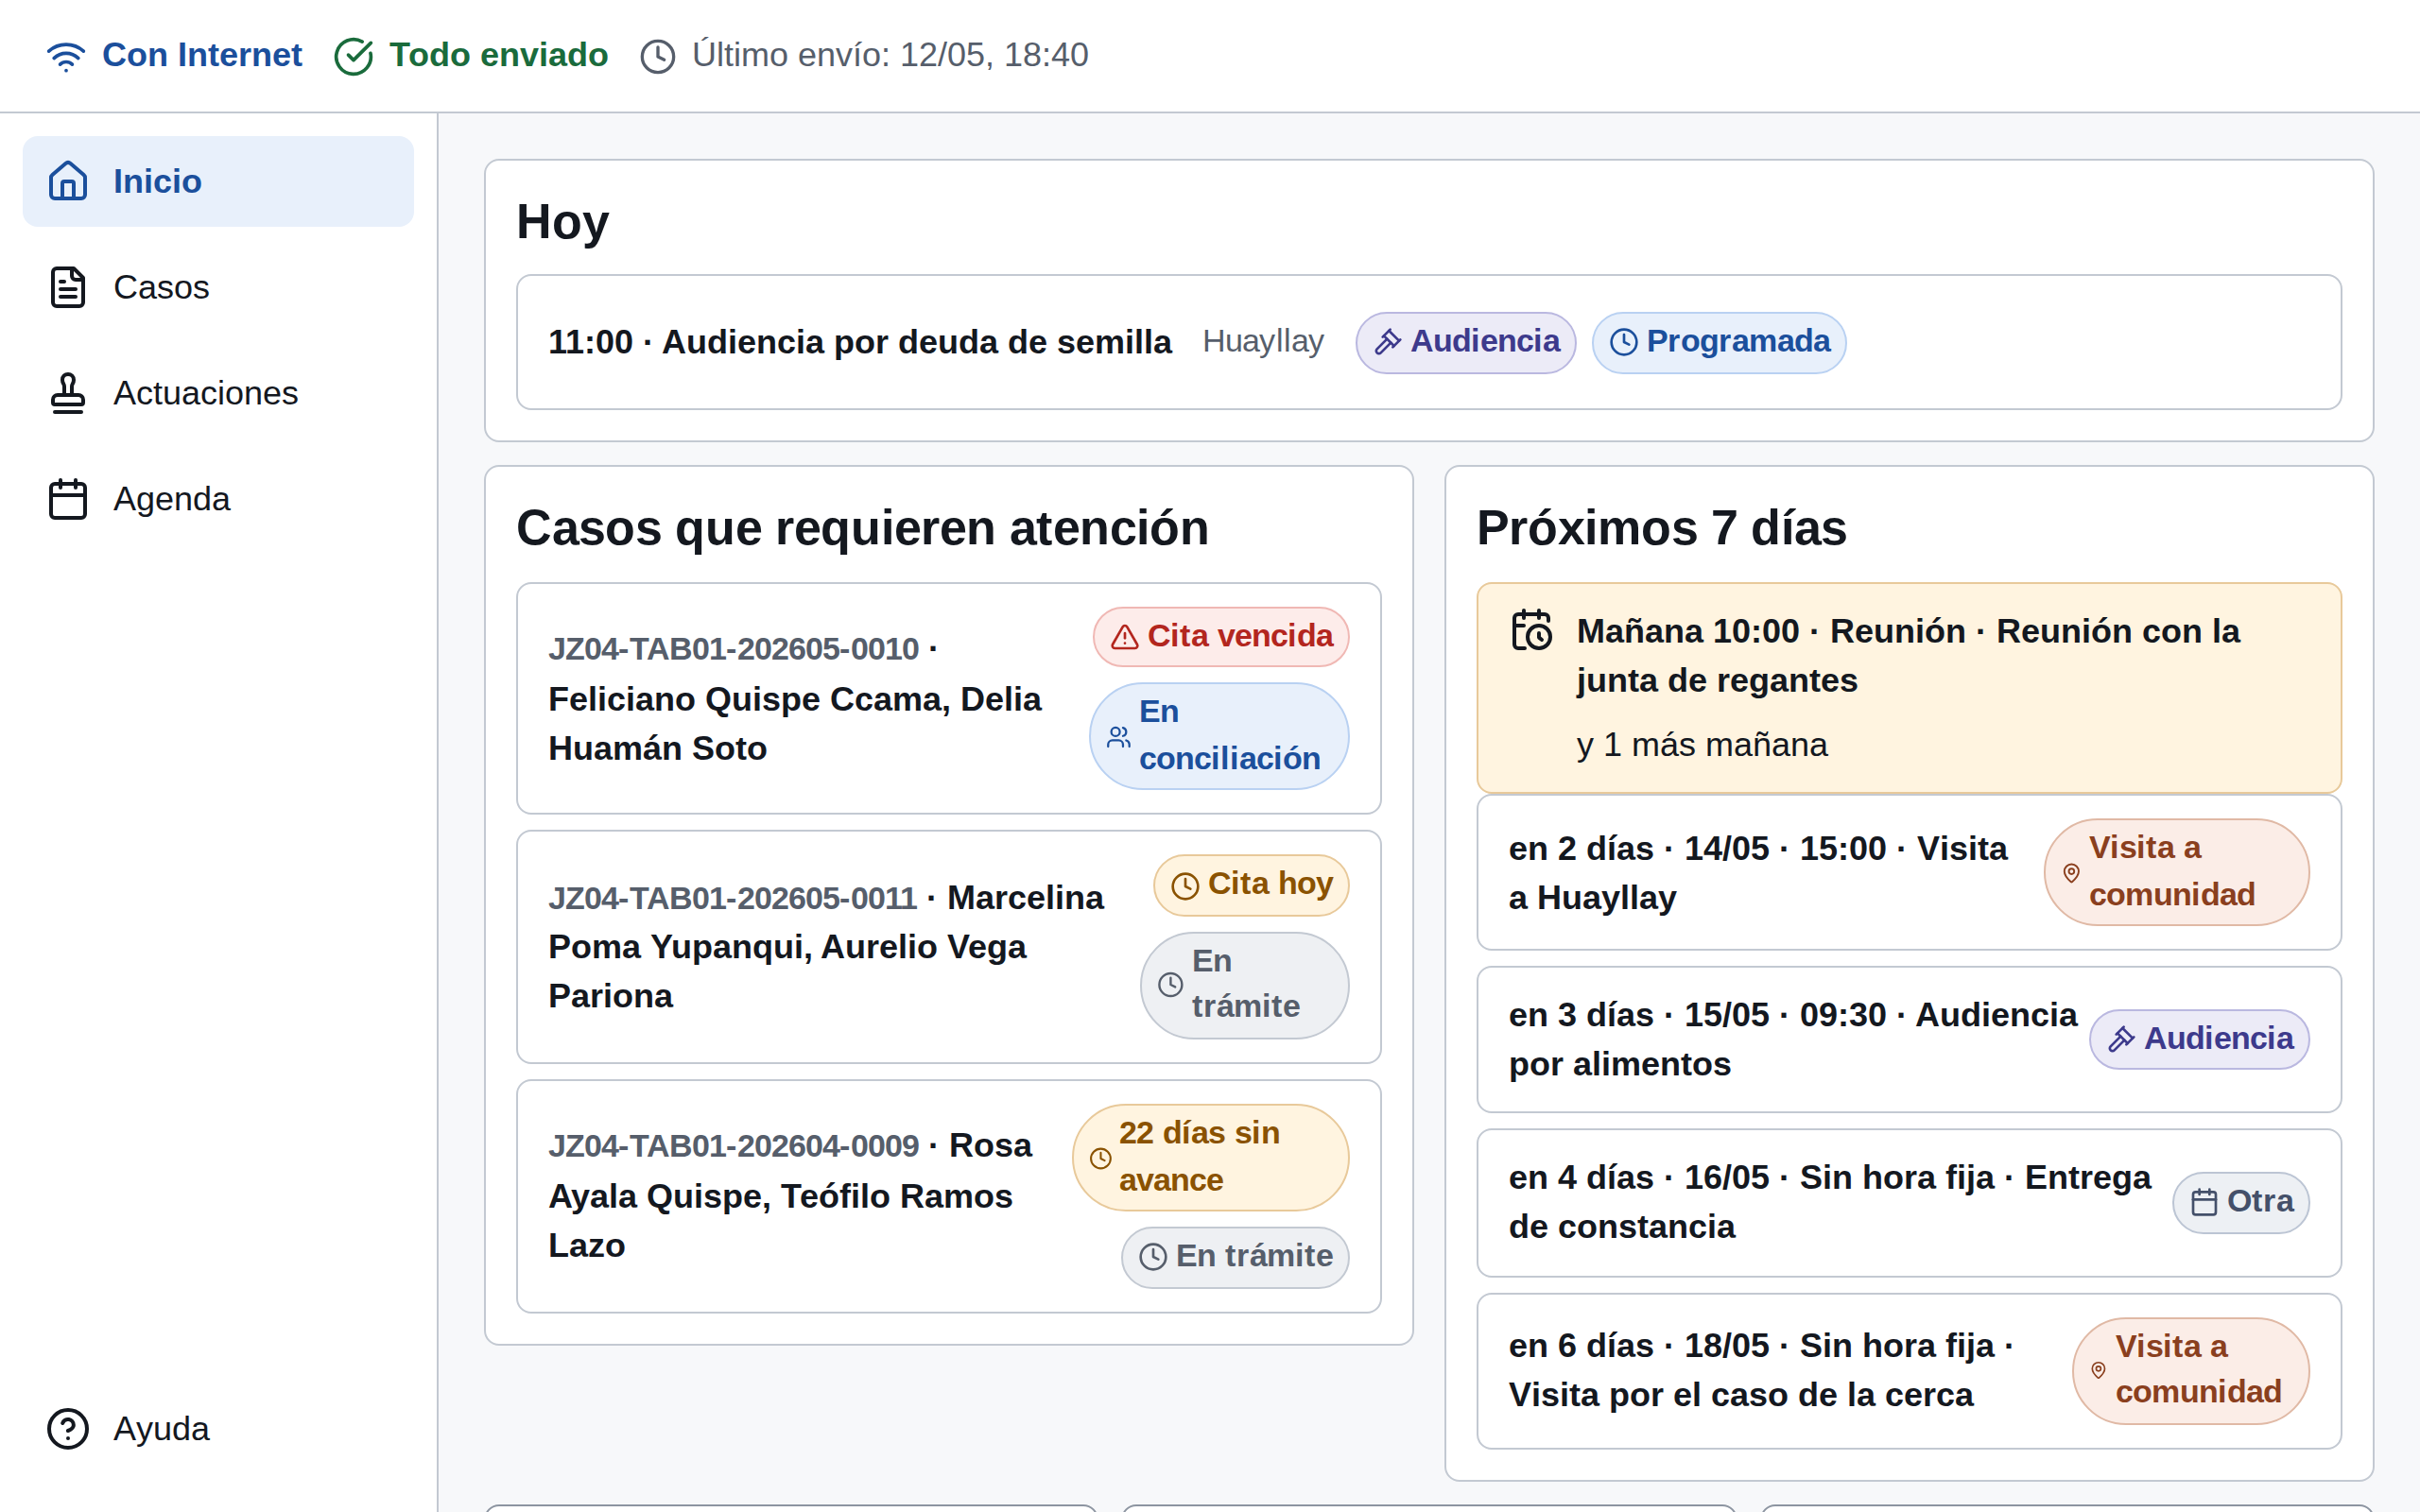
\includegraphics[width=0.78\linewidth]{capturas/BARRA-1_con-internet-todo-enviado.png}
\caption{P-01 · Con Internet y sin nada pendiente. Con Internet y sin nada pendiente}
\end{figure}
\begin{figure}[H]\centering
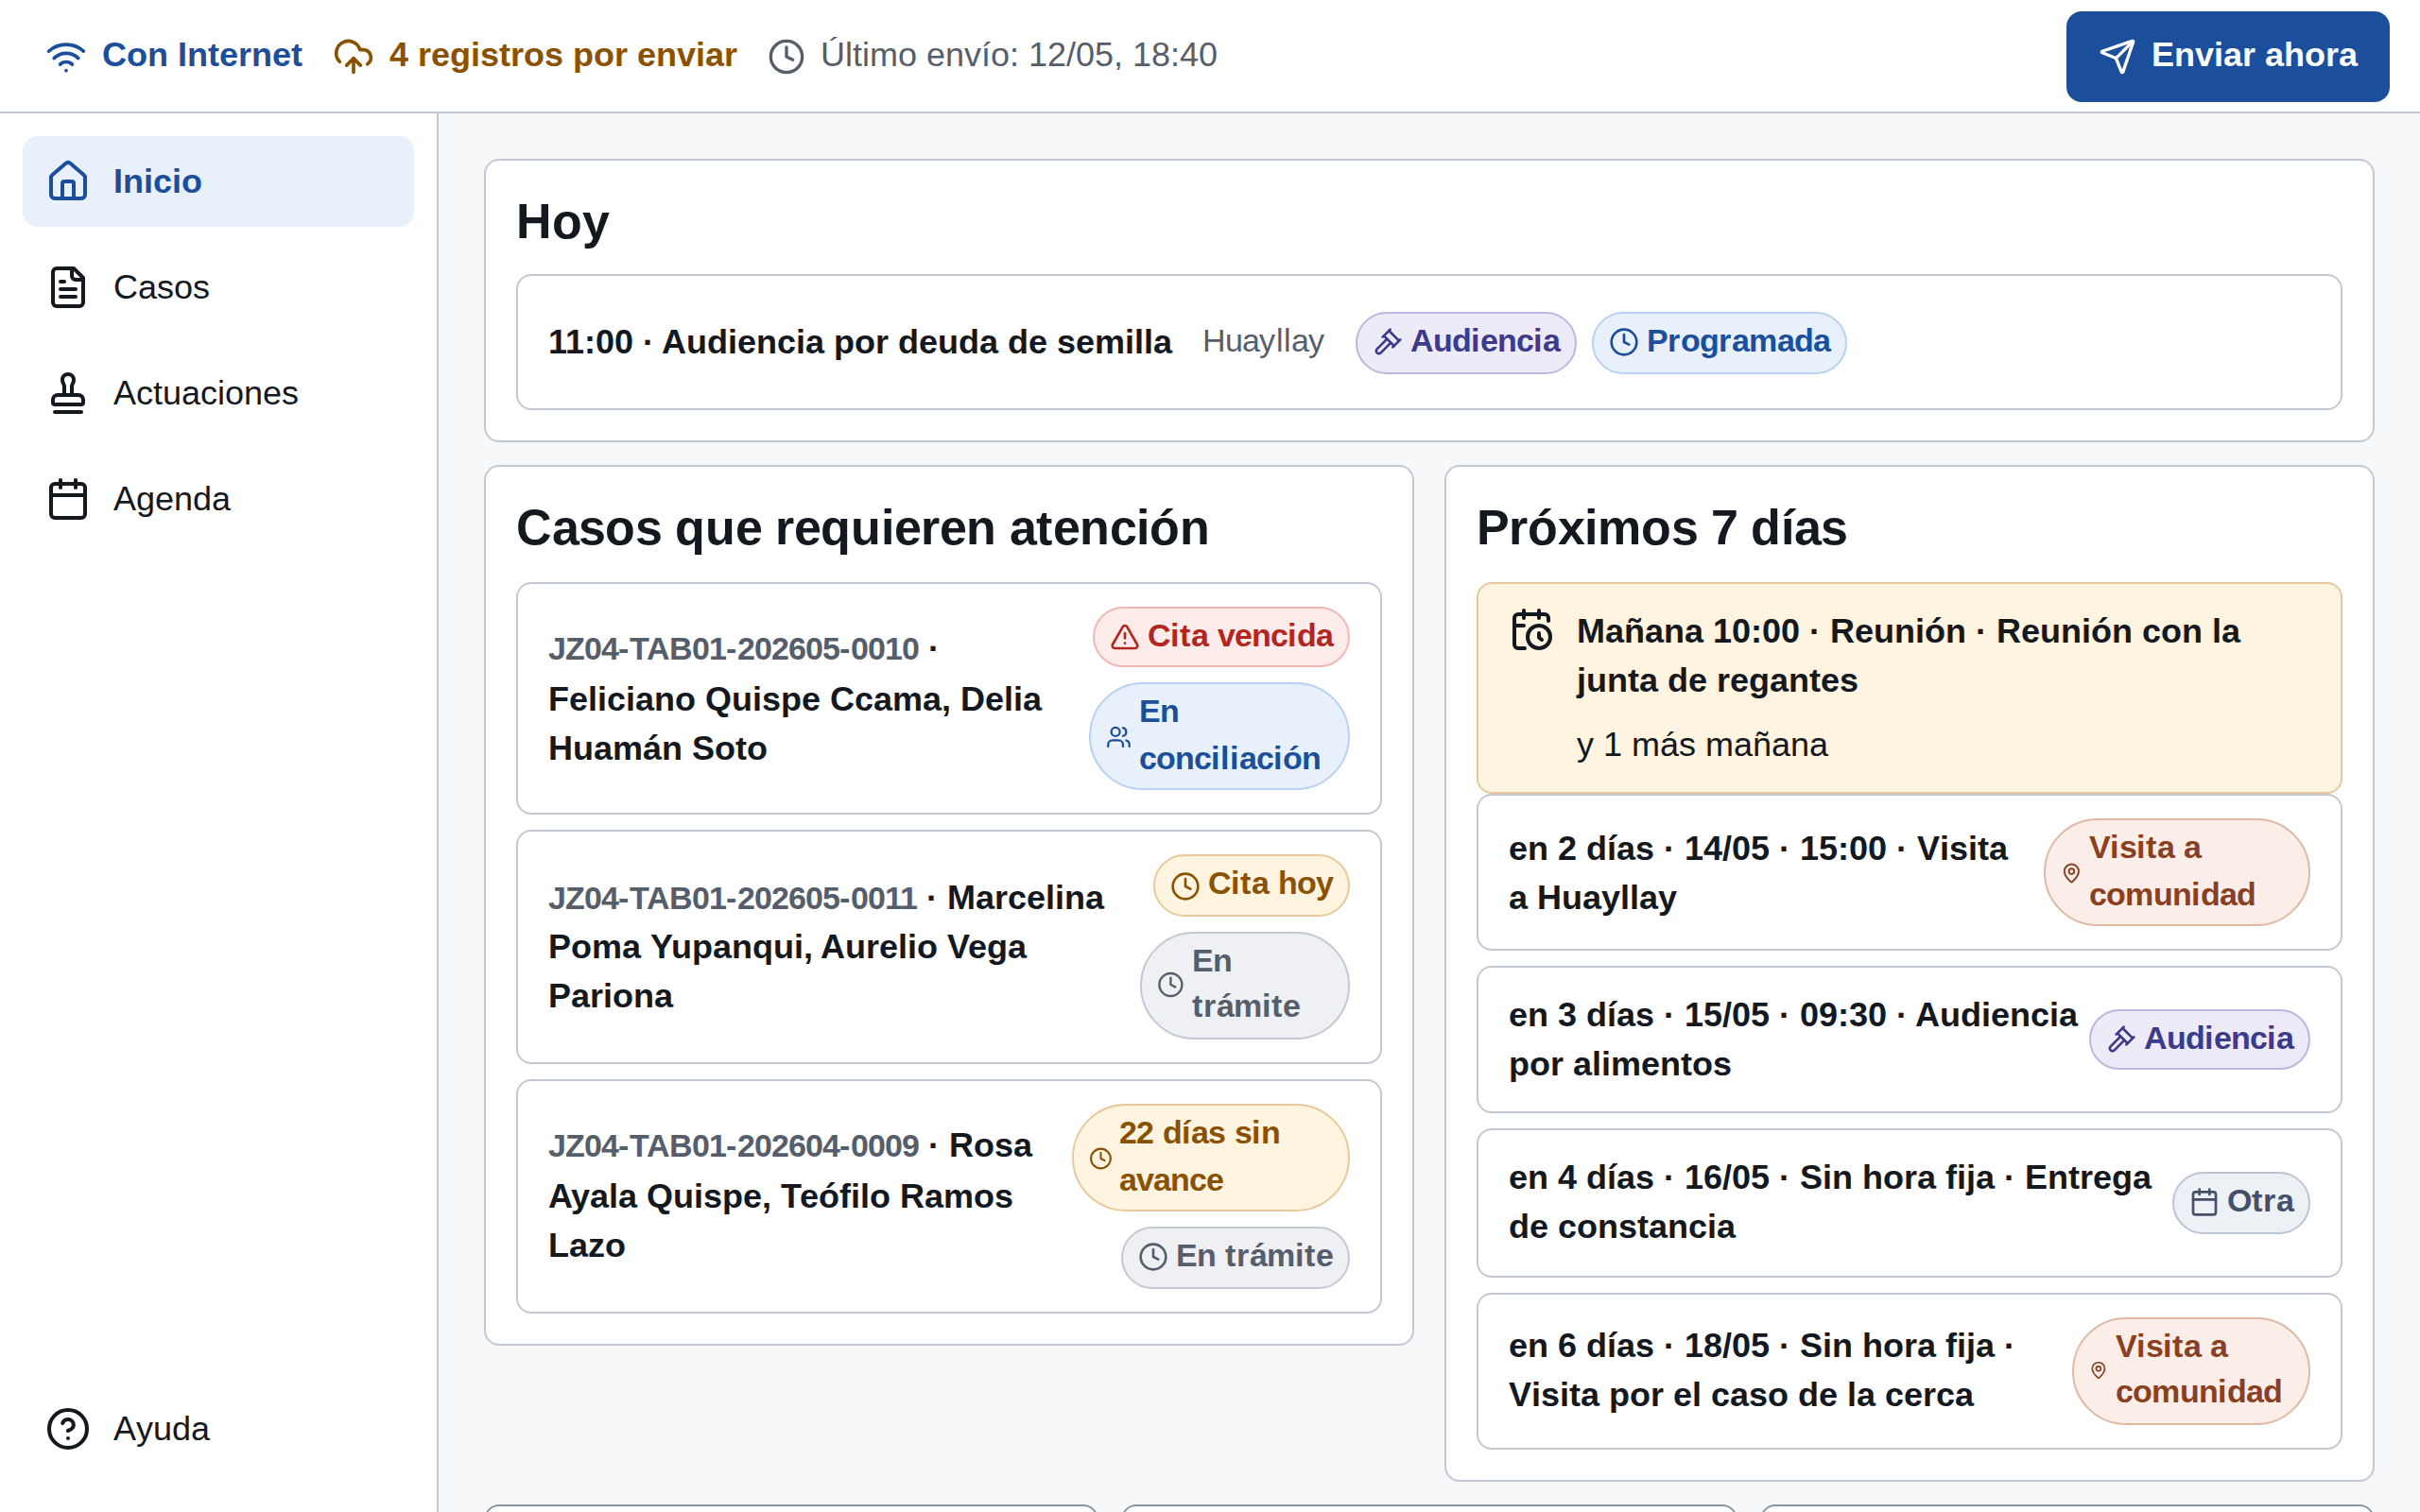
\includegraphics[width=0.78\linewidth]{capturas/BARRA-2_con-internet-pendientes.png}
\caption{P-01 · Con Internet y con registros por enviar. Con Internet y con registros por enviar: aparece el botón Enviar ahora}
\end{figure}
\begin{figure}[H]\centering
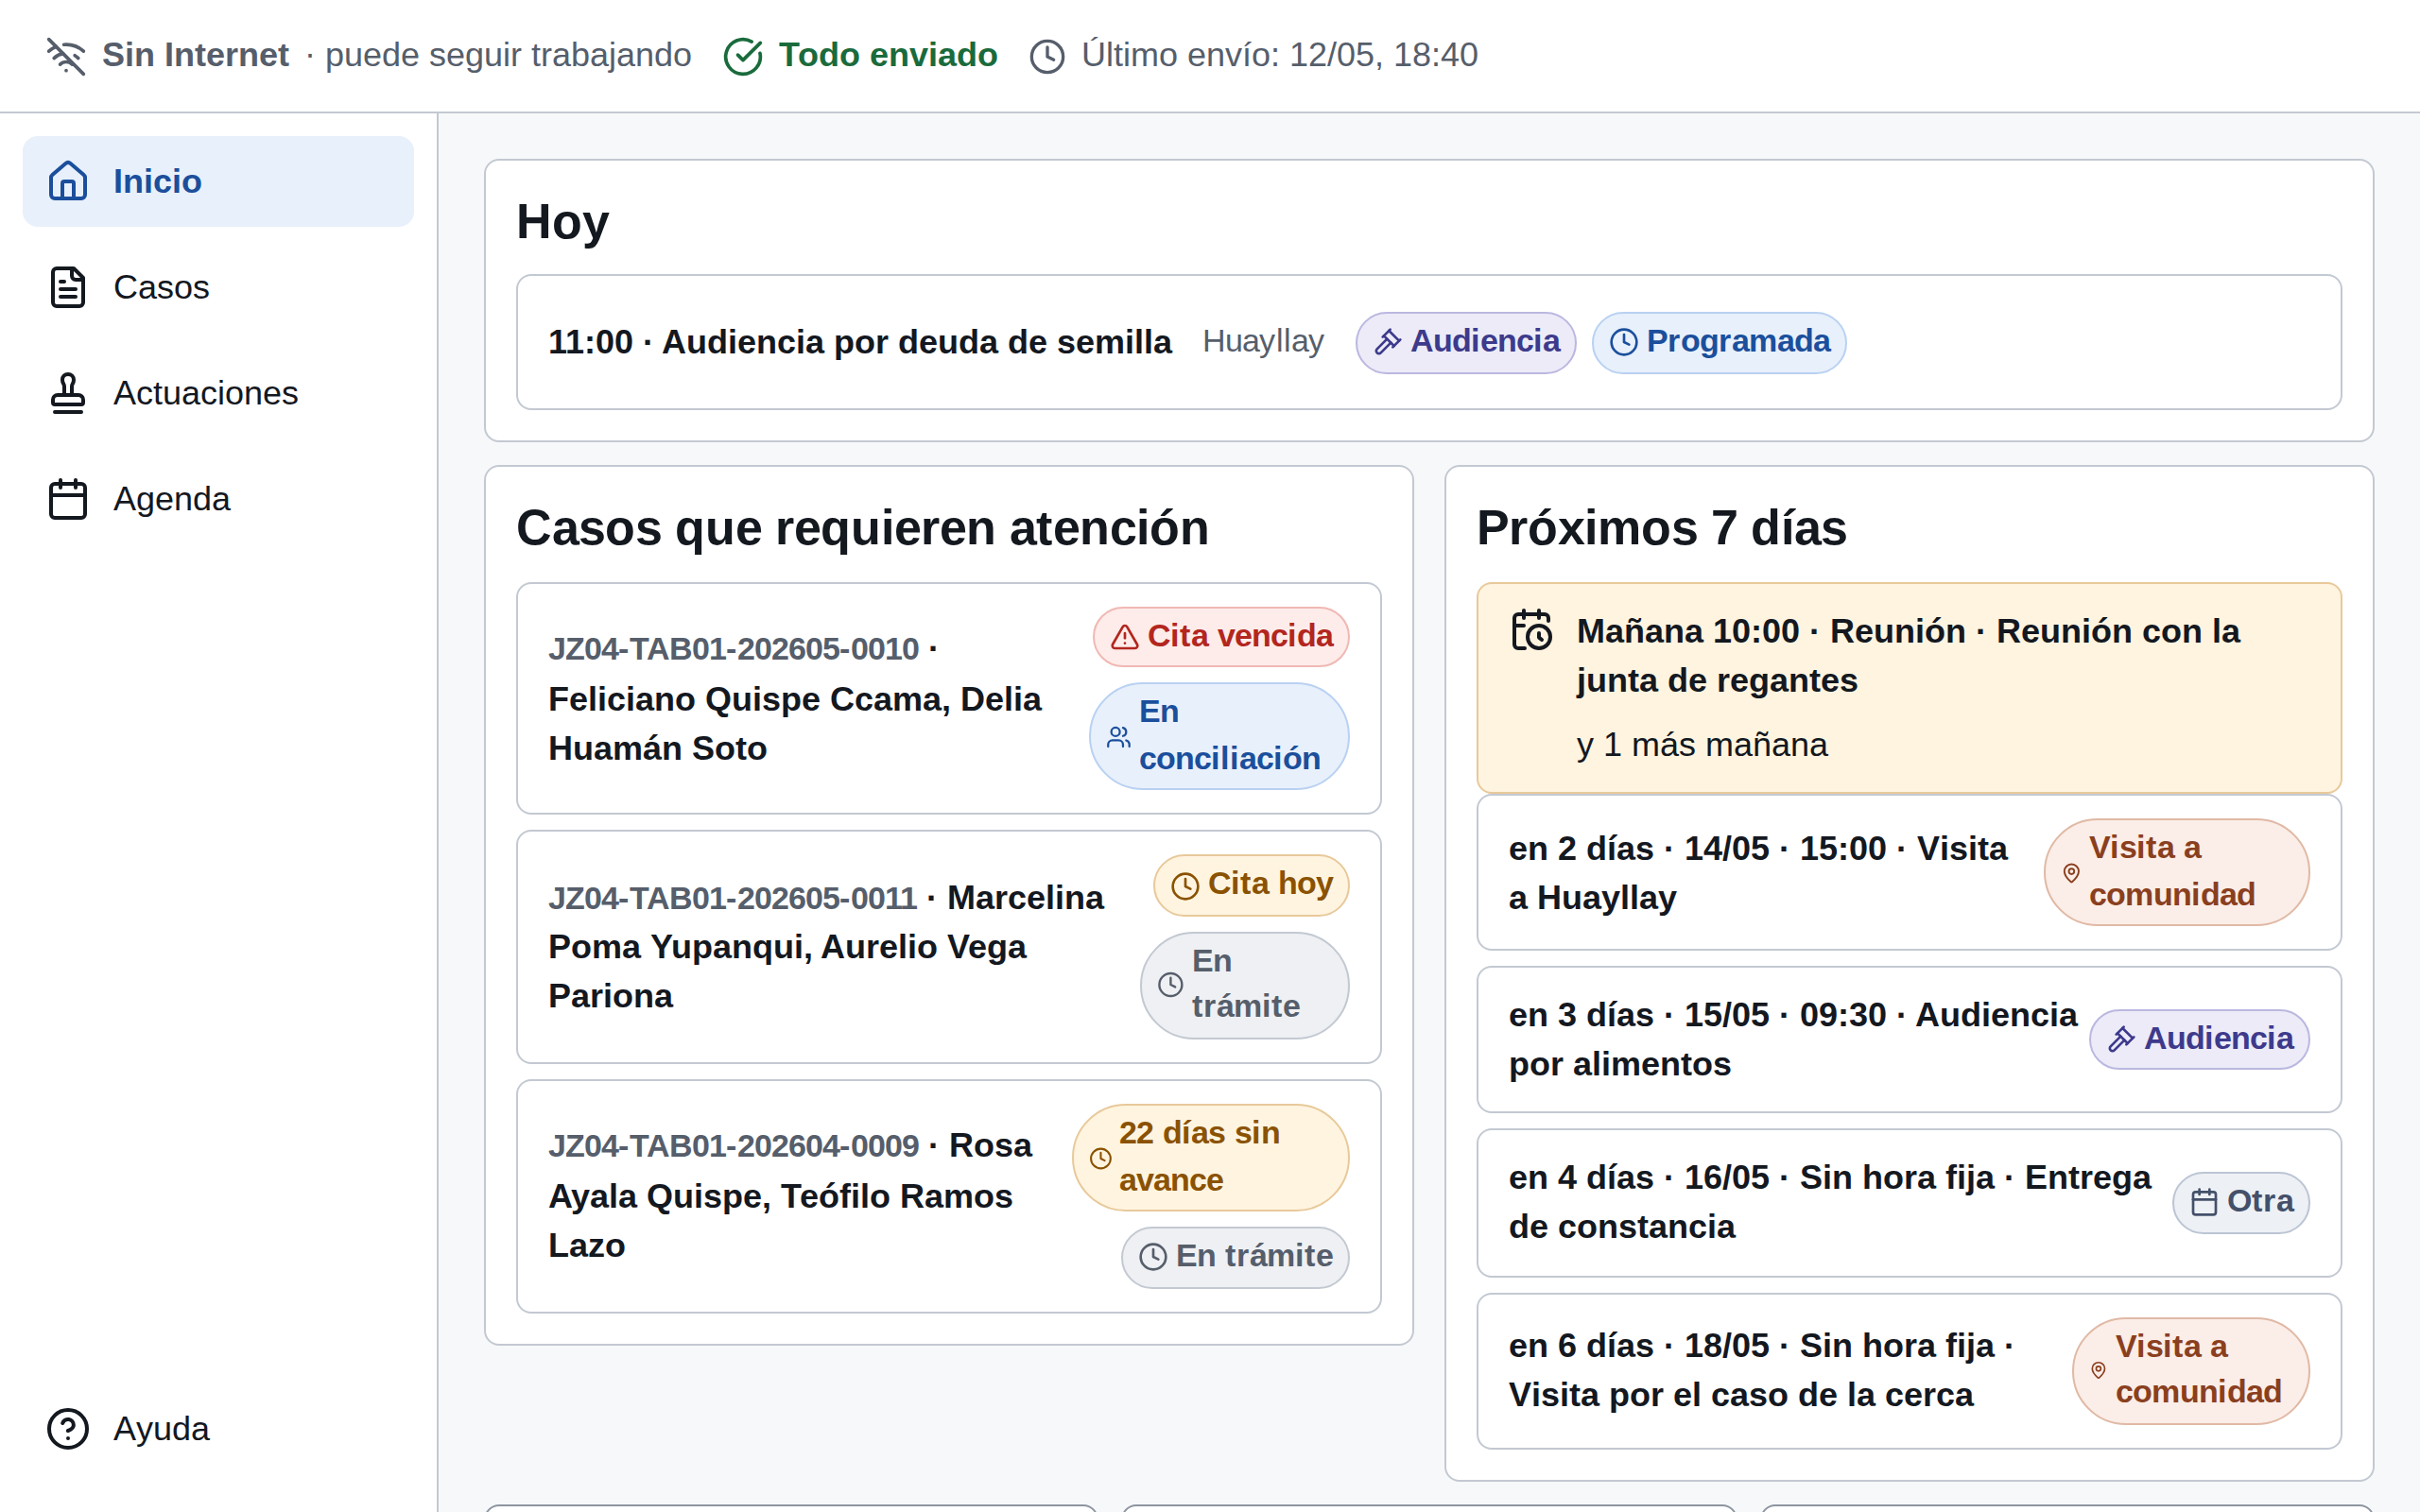
\includegraphics[width=0.78\linewidth]{capturas/BARRA-3_sin-internet-todo-enviado.png}
\caption{P-01 · Sin Internet en gris y sin nada pendiente. Sin Internet en gris y sin nada pendiente}
\end{figure}
\begin{figure}[H]\centering
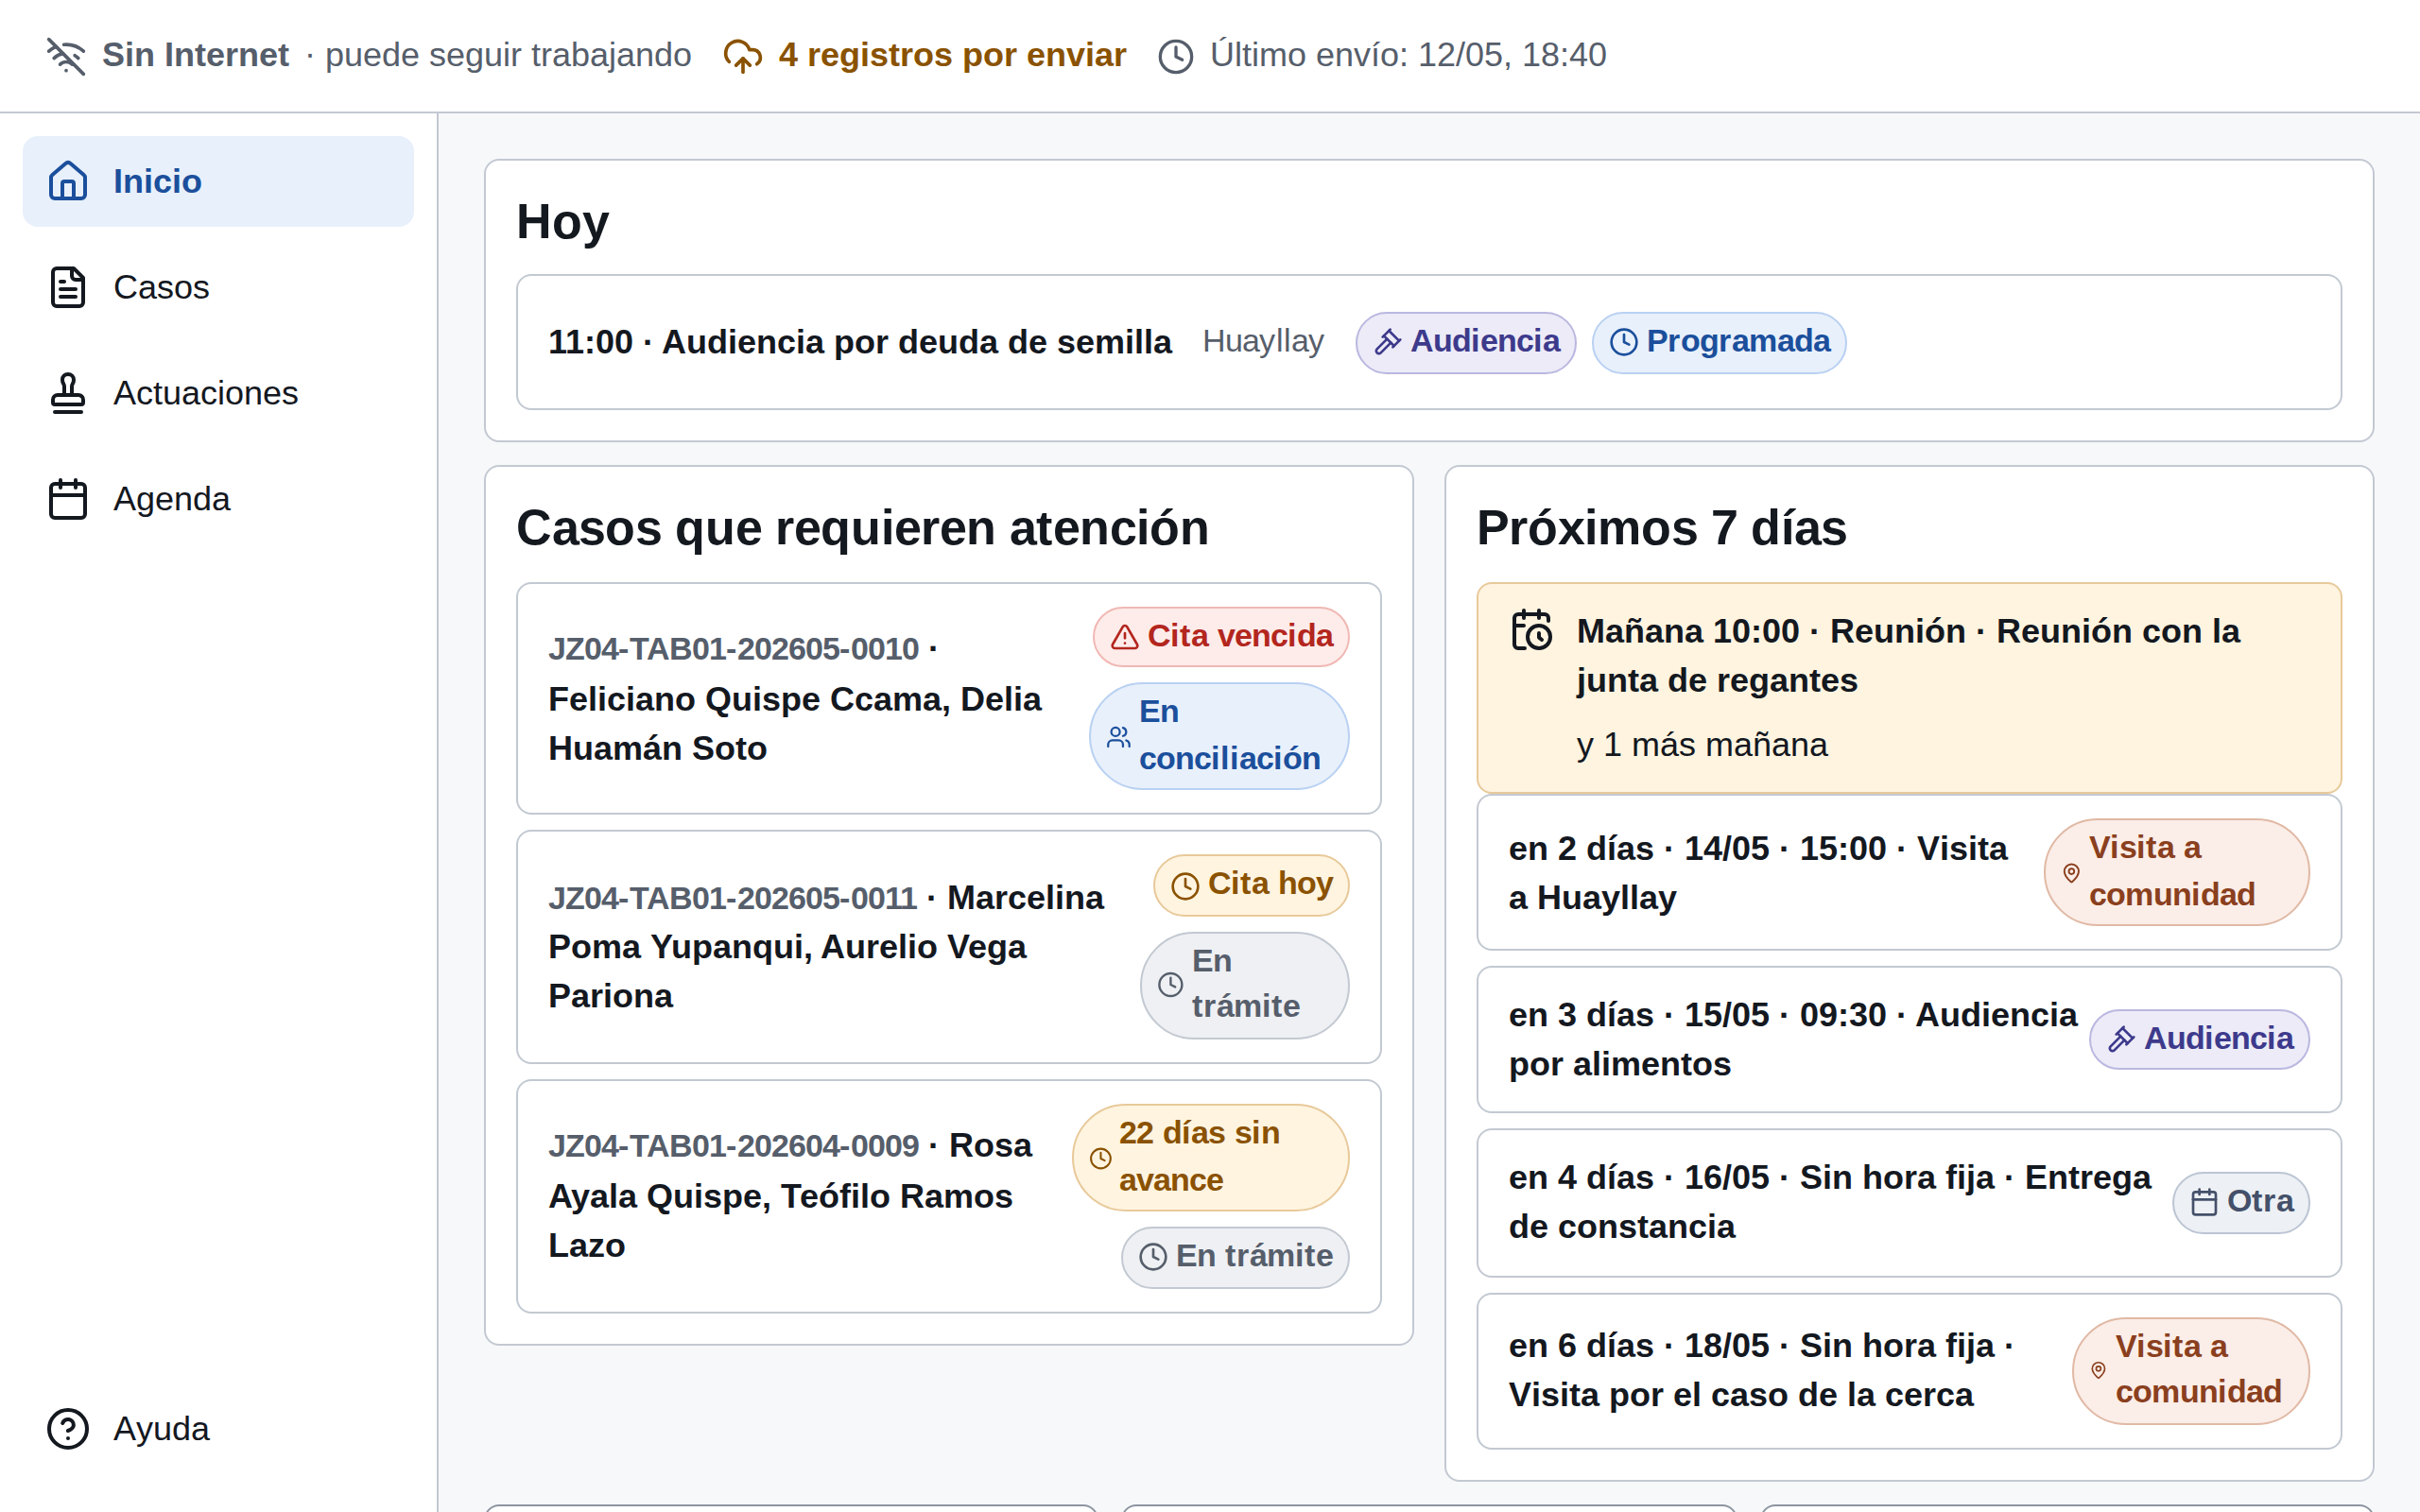
\includegraphics[width=0.78\linewidth]{capturas/BARRA-4_sin-internet-pendientes.png}
\caption{P-01 · Sin Internet en gris y con registros por enviar. Sin Internet en gris y con registros por enviar}
\end{figure}


\subsection{Distintivo por registro}

Cada caso, trámite y actividad lleva su propio distintivo, en la lista y en el detalle: \textbf{En la tableta} (ámbar, guardado y falta enviar), \textbf{Enviado} (verde) y \textbf{Revisar} (rojo, hubo un problema al enviarlo).

\subsection{Borrador y Completo, la misma regla en los tres módulos}

Todo registro tiene un estado propio (En trámite, Pendiente, Programada) y, aparte, un estado de registro: Borrador o Completo. Es automático: queda Completo cuando cumple sus mínimos. Siempre se puede guardar antes, y en la lista el borrador dice qué le falta: «Borrador · falta: personas». Los tres módulos tienen la casilla \textbf{Mostrar solo borradores}. Los borradores también se envían, marcados como tales, para no perder datos.

\subsection{Guardado automático y recuperación}

Los formularios guardan cada tres segundos y al salir de cada campo, con el texto discreto «Guardado automáticamente hace un momento». Si la aplicación se cierra, al volver a entrar ofrece continuar: «Tenía un caso sin terminar (Juan Quispe, 12/05). ¿Desea continuar?». Descartar pide confirmación.

Si pasan tres días o más con registros sin enviar, Inicio muestra el recordatorio con la consecuencia concreta: si la tableta se pierde o se daña, lo no enviado se perdería.

\subsection{Códigos generados en la tableta}

Los códigos se generan sin conexión y son definitivos: \texttt{JZ04-TAB01-202605-0013} para casos y \texttt{NOT-TAB01-202605-0007} para trámites. El prefijo de tableta evita que choquen con los que crea la computadora de la sede.

\subsection{Glosario de equivalencias con el enunciado}

\begin{center}
\begin{tabular}{@{}p{7.2cm}p{7.6cm}@{}}
\toprule
\textbf{Lo que dice la interfaz} & \textbf{Lo que pide el enunciado} \\
\midrule
«4 registros por enviar» & Sincronización pendiente \\
«Enviar al Poder Judicial», «Enviar ahora» & Sincronizar \\
«Guardado en la tableta», «En la tableta» & Almacenamiento local \\
«Sin Internet · puede seguir trabajando» & Modo sin conexión \\
«Se usó la versión de la computadora» & Resolución de conflictos \\
\bottomrule
\end{tabular}
\end{center}

La columna de la izquierda es la única que ve la jueza. La de la derecha no aparece en ninguna pantalla.

\section{Bocetos a mano alzada}

El diseño empezó en papel cuadriculado. Los tres bocetos de esta sección se dibujaron antes de
escribir una línea de código, y sirven para ver qué decisiones venían de la idea original y cuáles
aparecieron al construir el prototipo.

\subsection{Inicio}

\begin{figure}[H]\centering
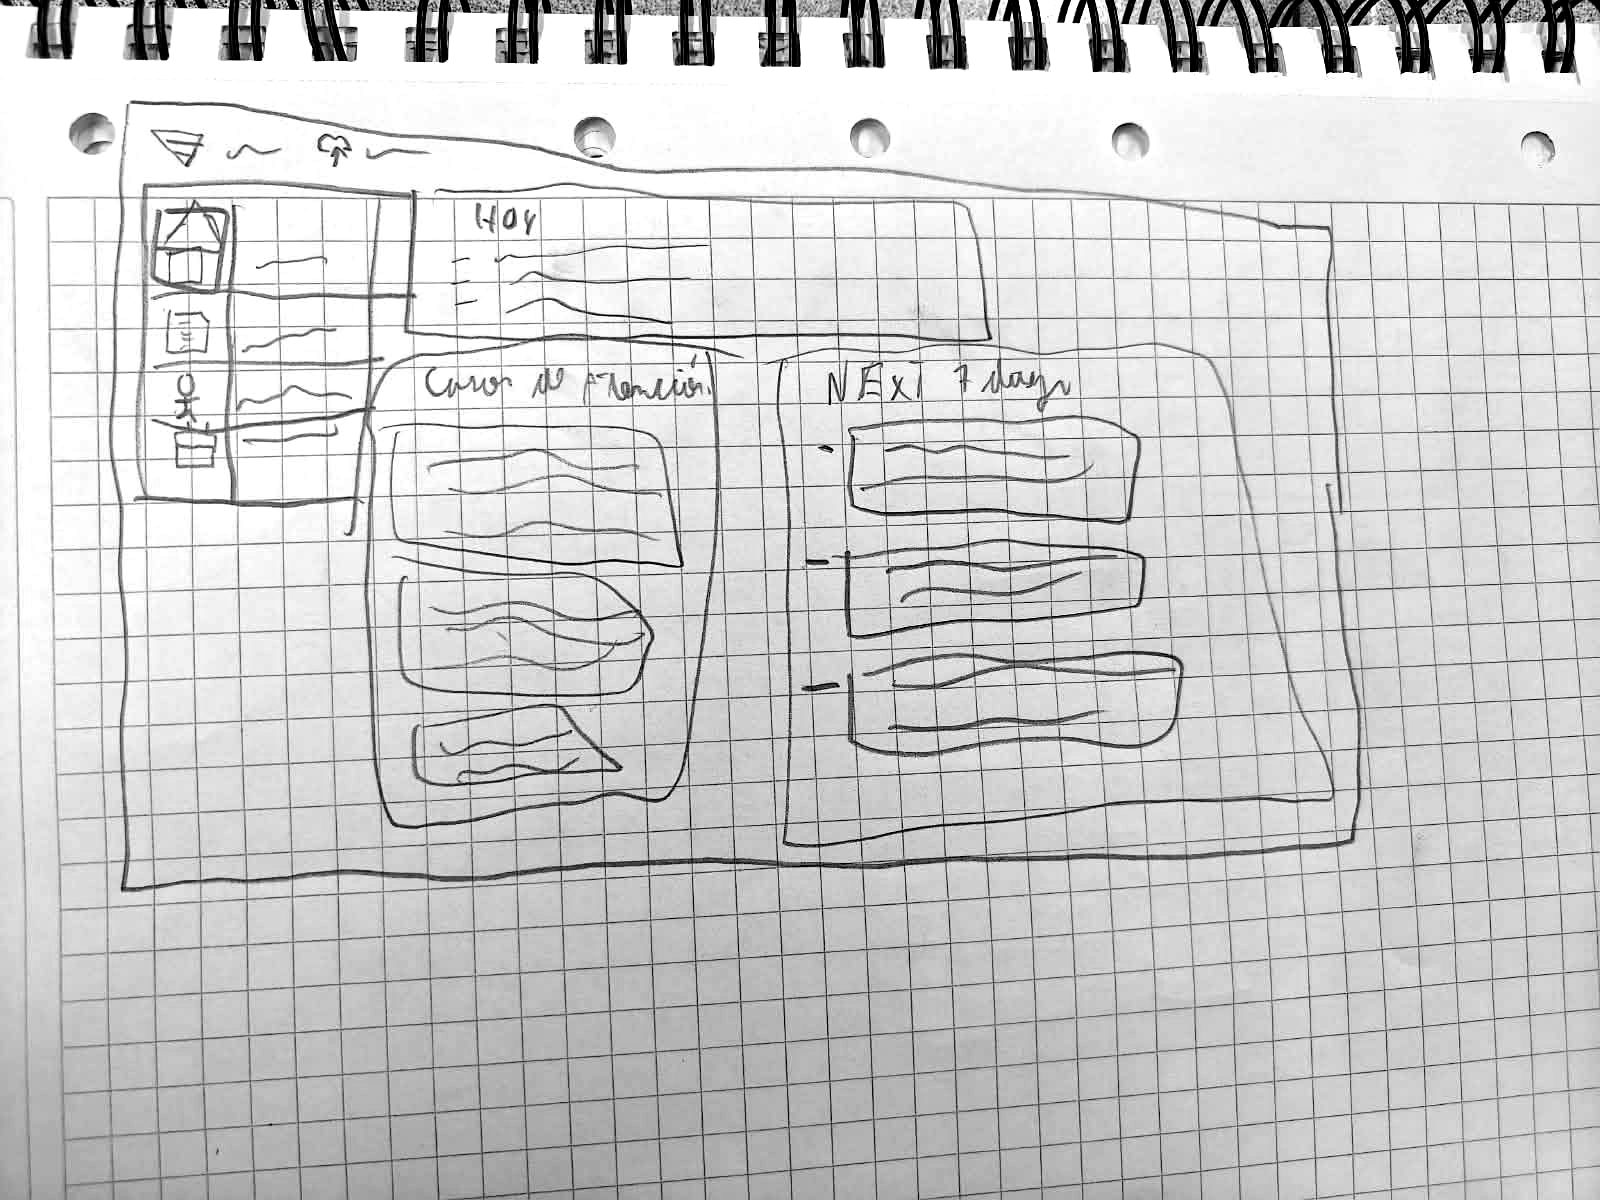
\includegraphics[width=0.84\linewidth]{bocetos/boceto-inicio.jpg}
\caption{Boceto de la pantalla de Inicio: barra de estado arriba, menú lateral de cuatro opciones con ícono y texto, «Hoy» a lo ancho, y debajo dos columnas: casos que requieren atención y los próximos 7 días.}
\end{figure}

El esqueleto se mantuvo tal cual: la barra de estado ocupa todo el ancho arriba, el menú lateral tiene
cuatro opciones y el cuerpo reparte «Hoy» a lo ancho con las dos columnas debajo. Lo que se añadió
después son los tres accesos grandes del final (Nuevo caso, Nueva actuación, Nueva actividad), que en
el boceto no existían: al recorrer el flujo completo se vio que la jueza empieza a registrar mientras
la persona todavía está hablando, y desde Inicio eso costaba dos toques en vez de uno.

\subsection{Casos y Actuaciones}

\begin{figure}[H]\centering
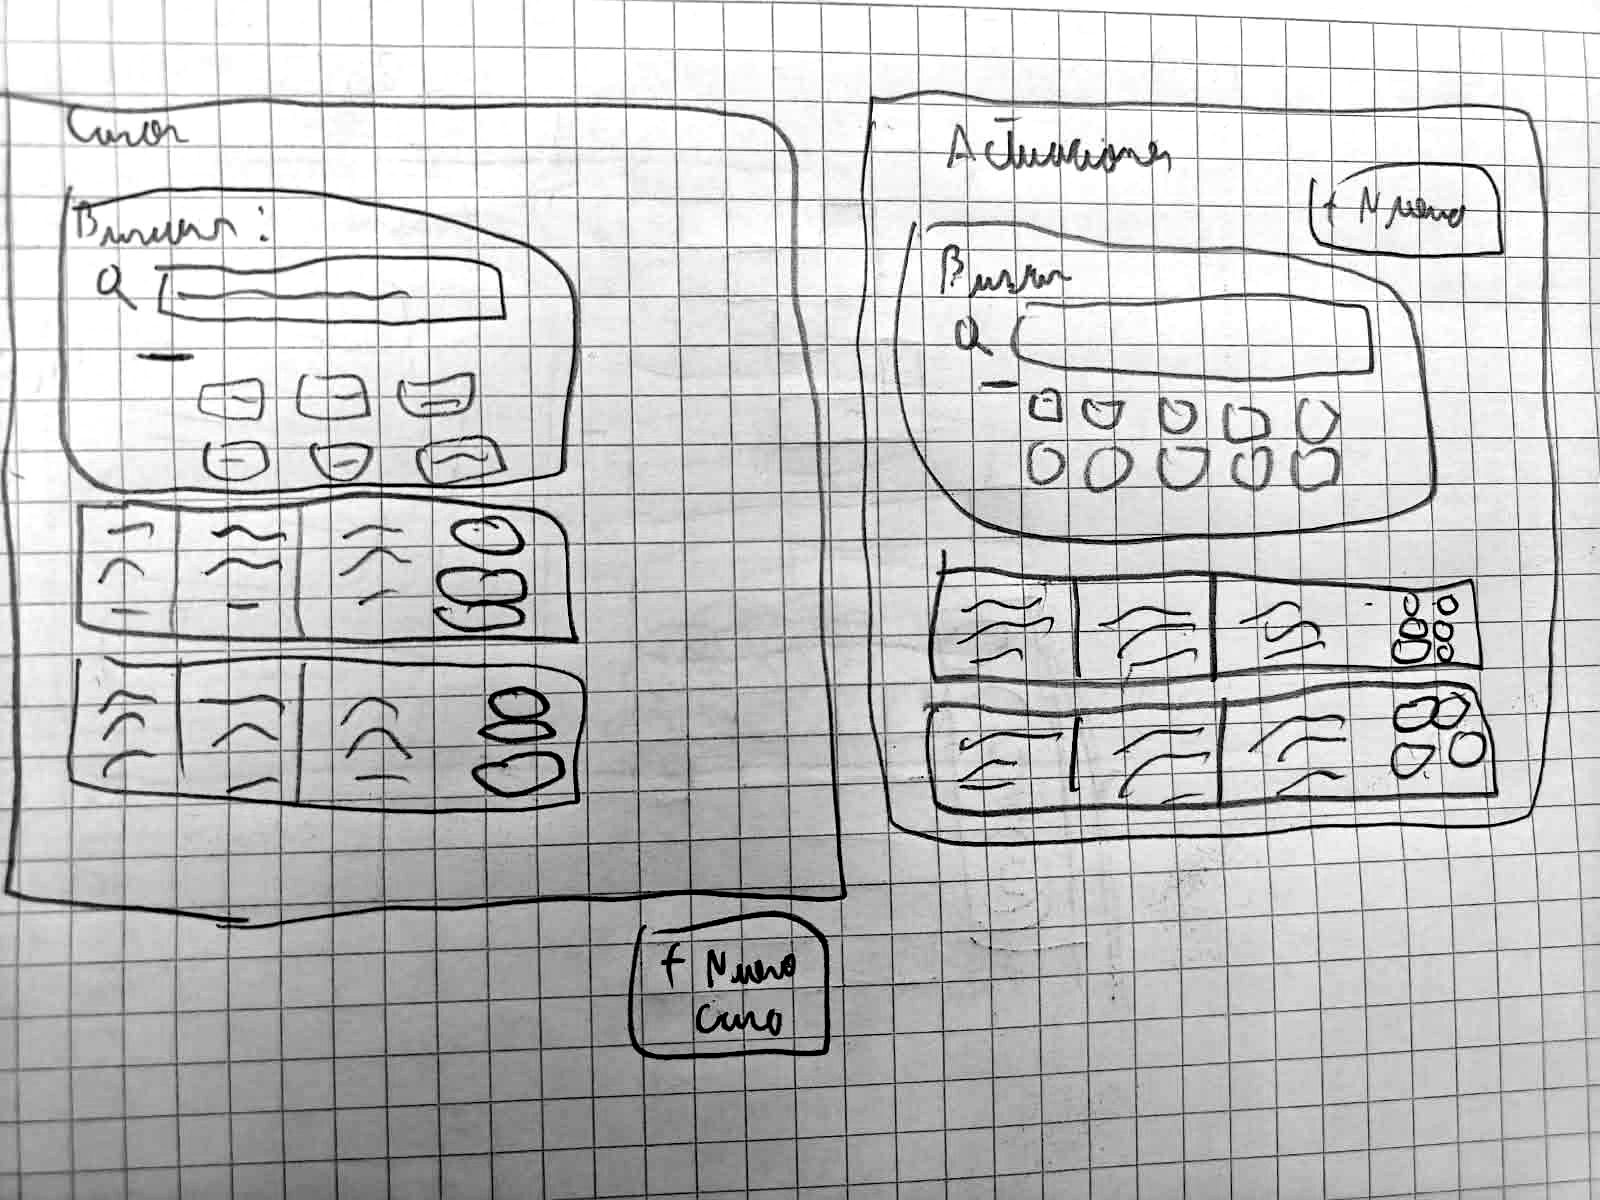
\includegraphics[width=0.84\linewidth]{bocetos/boceto-casos.jpg}
\caption{Boceto de las dos listas: buscador con lupa, una fila de filtros en botones, las filas del listado con sus marcas al final, y el botón de registro nuevo.}
\end{figure}

De aquí salió que los filtros fueran botones visibles y no listas desplegables, y que cada fila
terminara en sus marcas de estado. Dos cosas cambiaron. La primera: en el boceto el botón de registro
nuevo está abajo a la derecha en Casos y arriba a la derecha en Actuaciones; en el prototipo los dos
quedaron abajo a la derecha, porque una acción que cambia de sitio entre dos pantallas gemelas obliga
a buscarla cada vez (H4, consistencia). La segunda: los filtros del boceto eran una sola fila de
botones sin rótulo, y al llenarlos con datos reales hubo que agruparlos y nombrarlos (Comunidad,
Estado, Tipo) y añadir la casilla «Mostrar solo borradores», que no estaba prevista.

\subsection{Agenda}

\begin{figure}[H]\centering
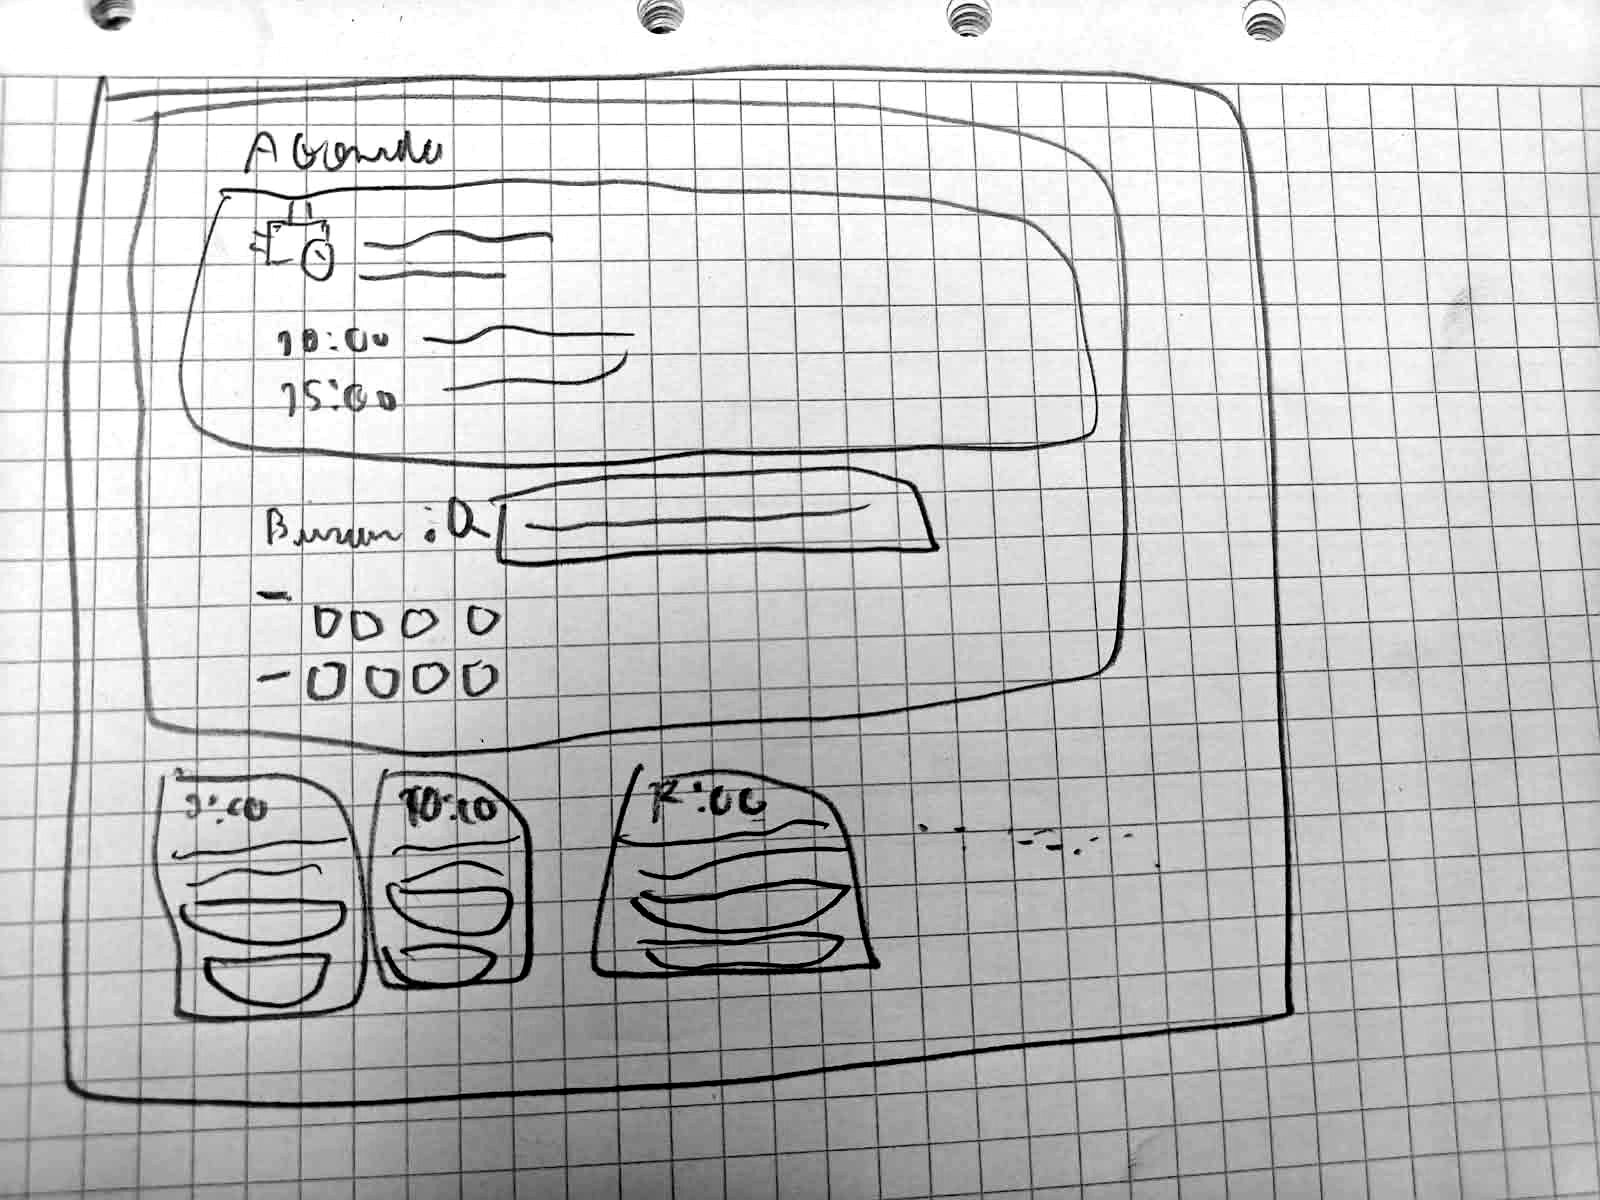
\includegraphics[width=0.84\linewidth]{bocetos/boceto-agenda.jpg}
\caption{Boceto de la Agenda: aviso de lo próximo con sus horas arriba, buscador, dos filas de filtros y las actividades del día en tarjetas por hora.}
\end{figure}

El aviso de lo próximo con la hora al frente, el buscador y las tarjetas por hora pasaron al prototipo
sin cambios. Lo que se agregó es el selector Mes, Semana y Día: el boceto resolvía un solo nivel de
detalle, y al probar el flujo de la semana quedó claro que planificar un viaje a una comunidad lejana
necesita ver el mes entero, mientras que preparar una audiencia necesita ver el día.

\section{Ingreso y primeras pantallas}

\begin{figure}[H]\centering
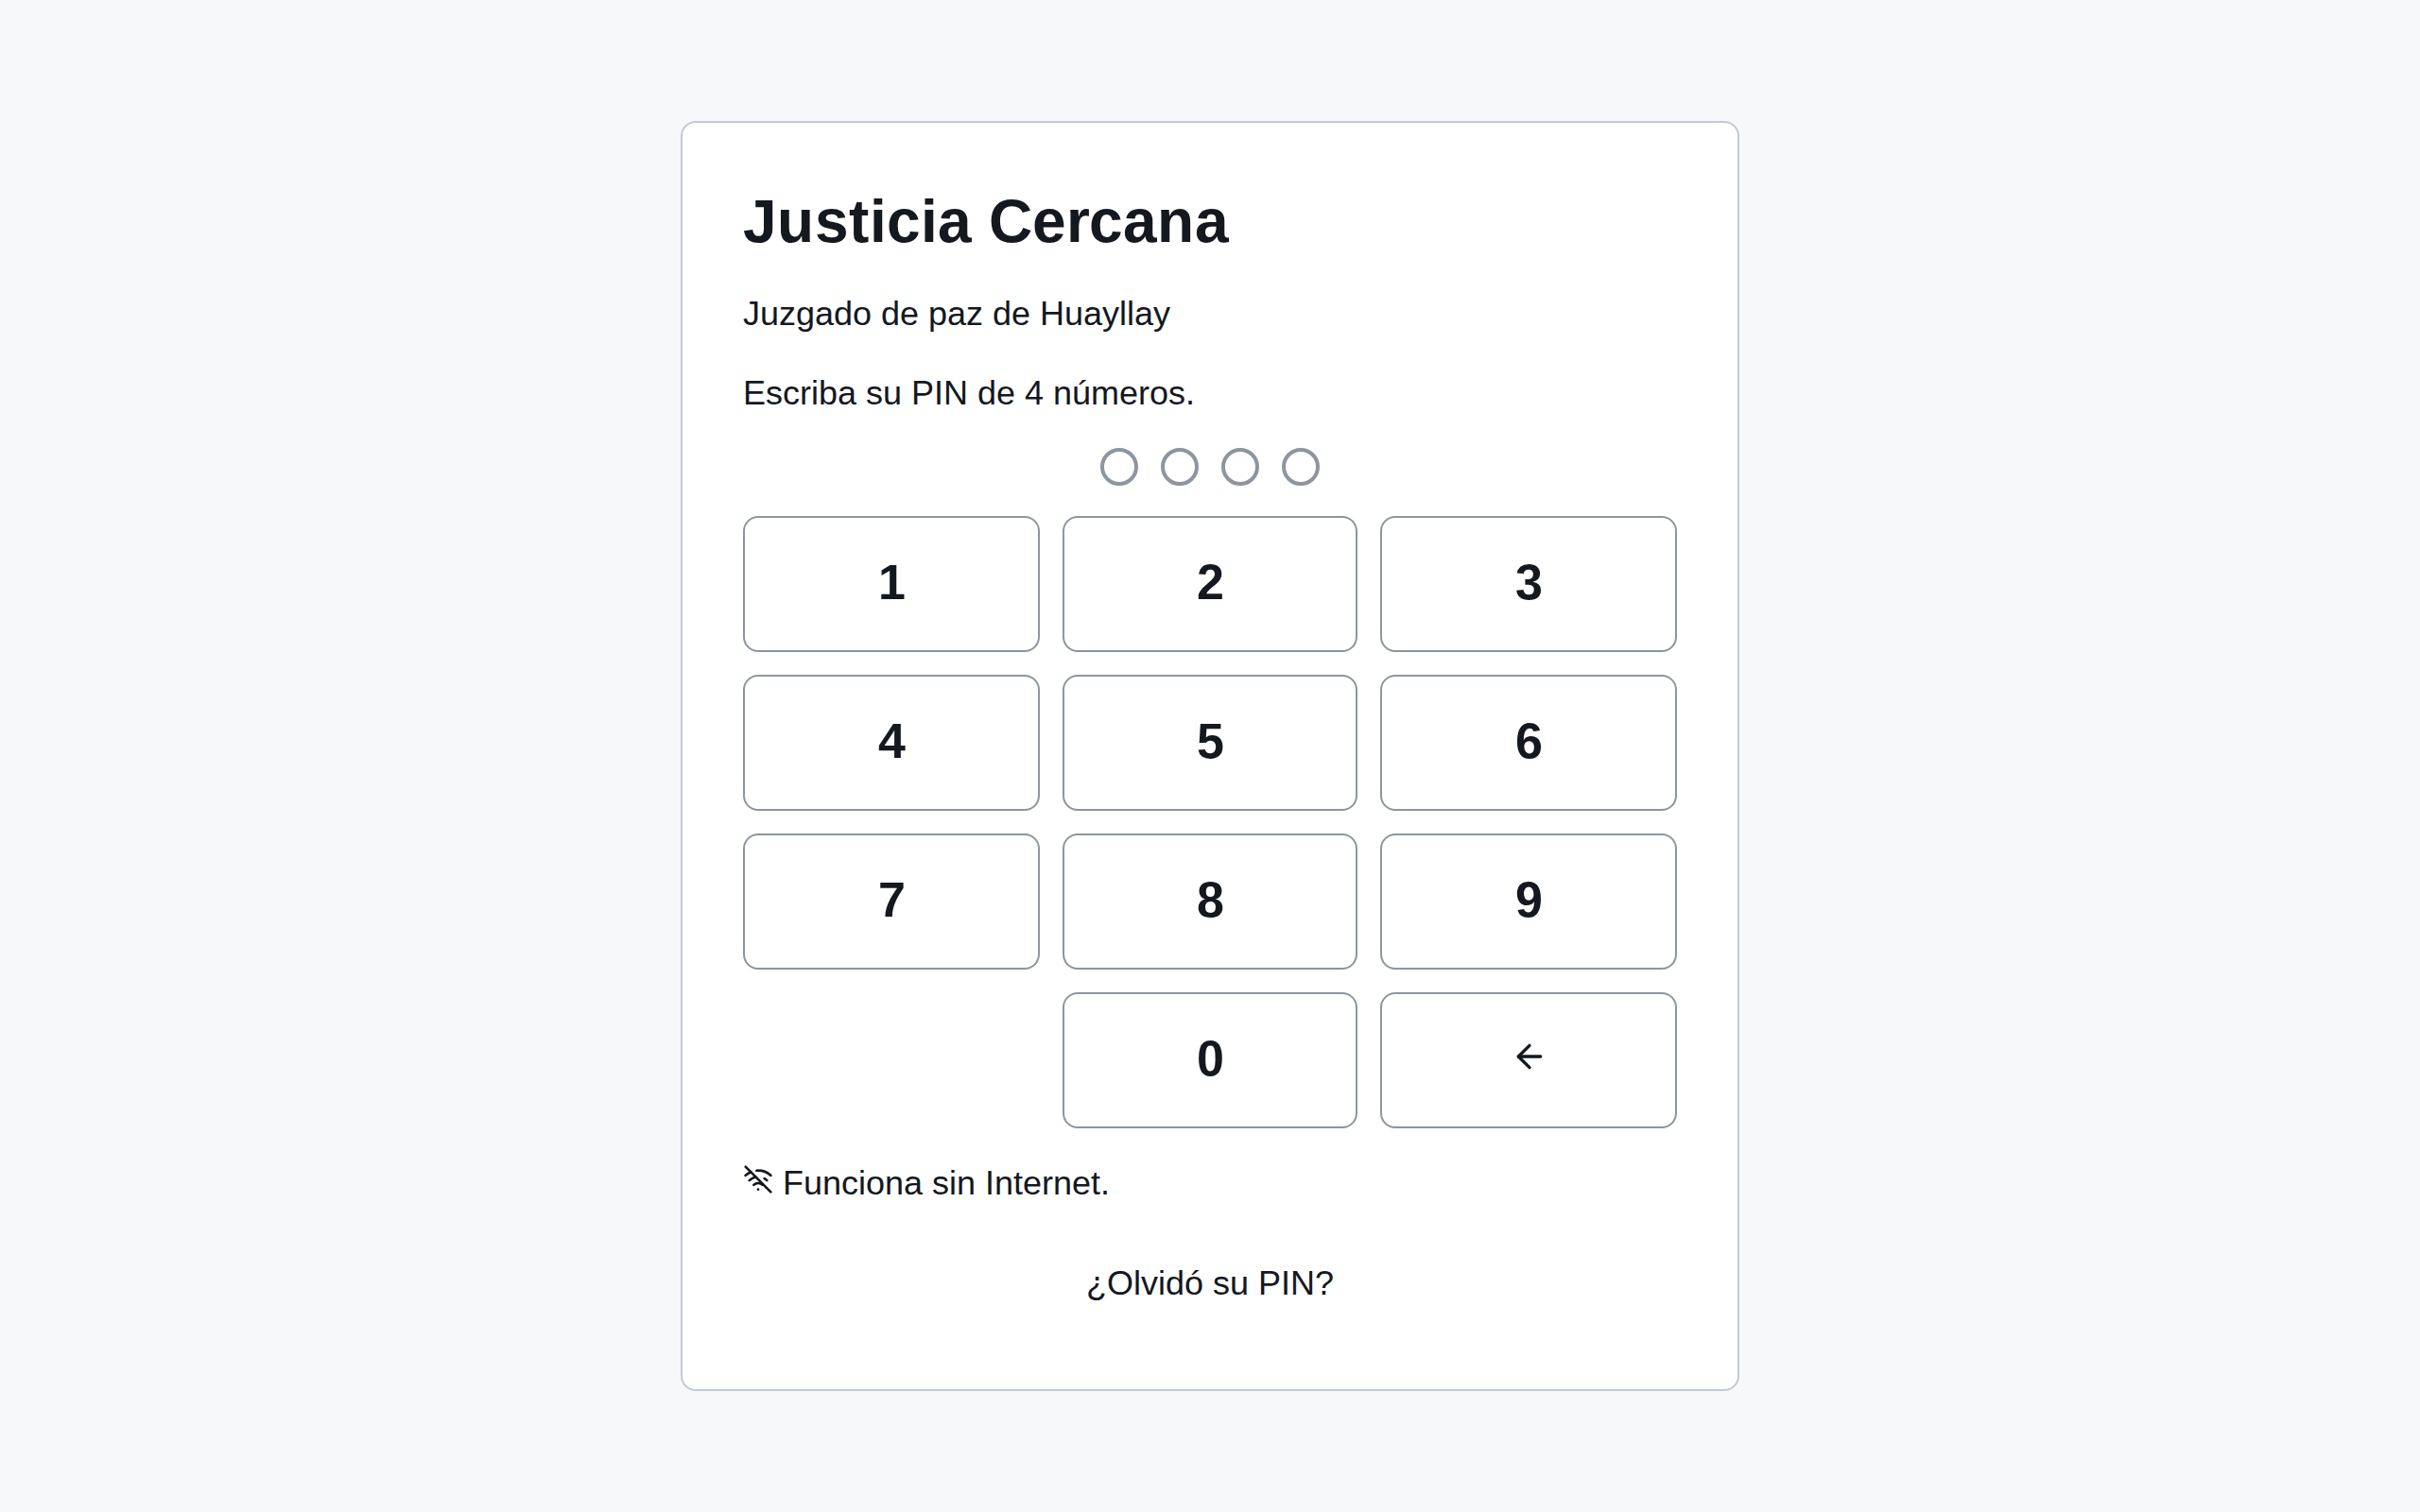
\includegraphics[width=0.86\linewidth]{capturas/P-00_ingreso-pin.png}
\caption{P-00 · Ingreso. PIN numérico de 4 dígitos con teclado grande, funciona sin Internet}
\end{figure}
\begin{figure}[H]\centering
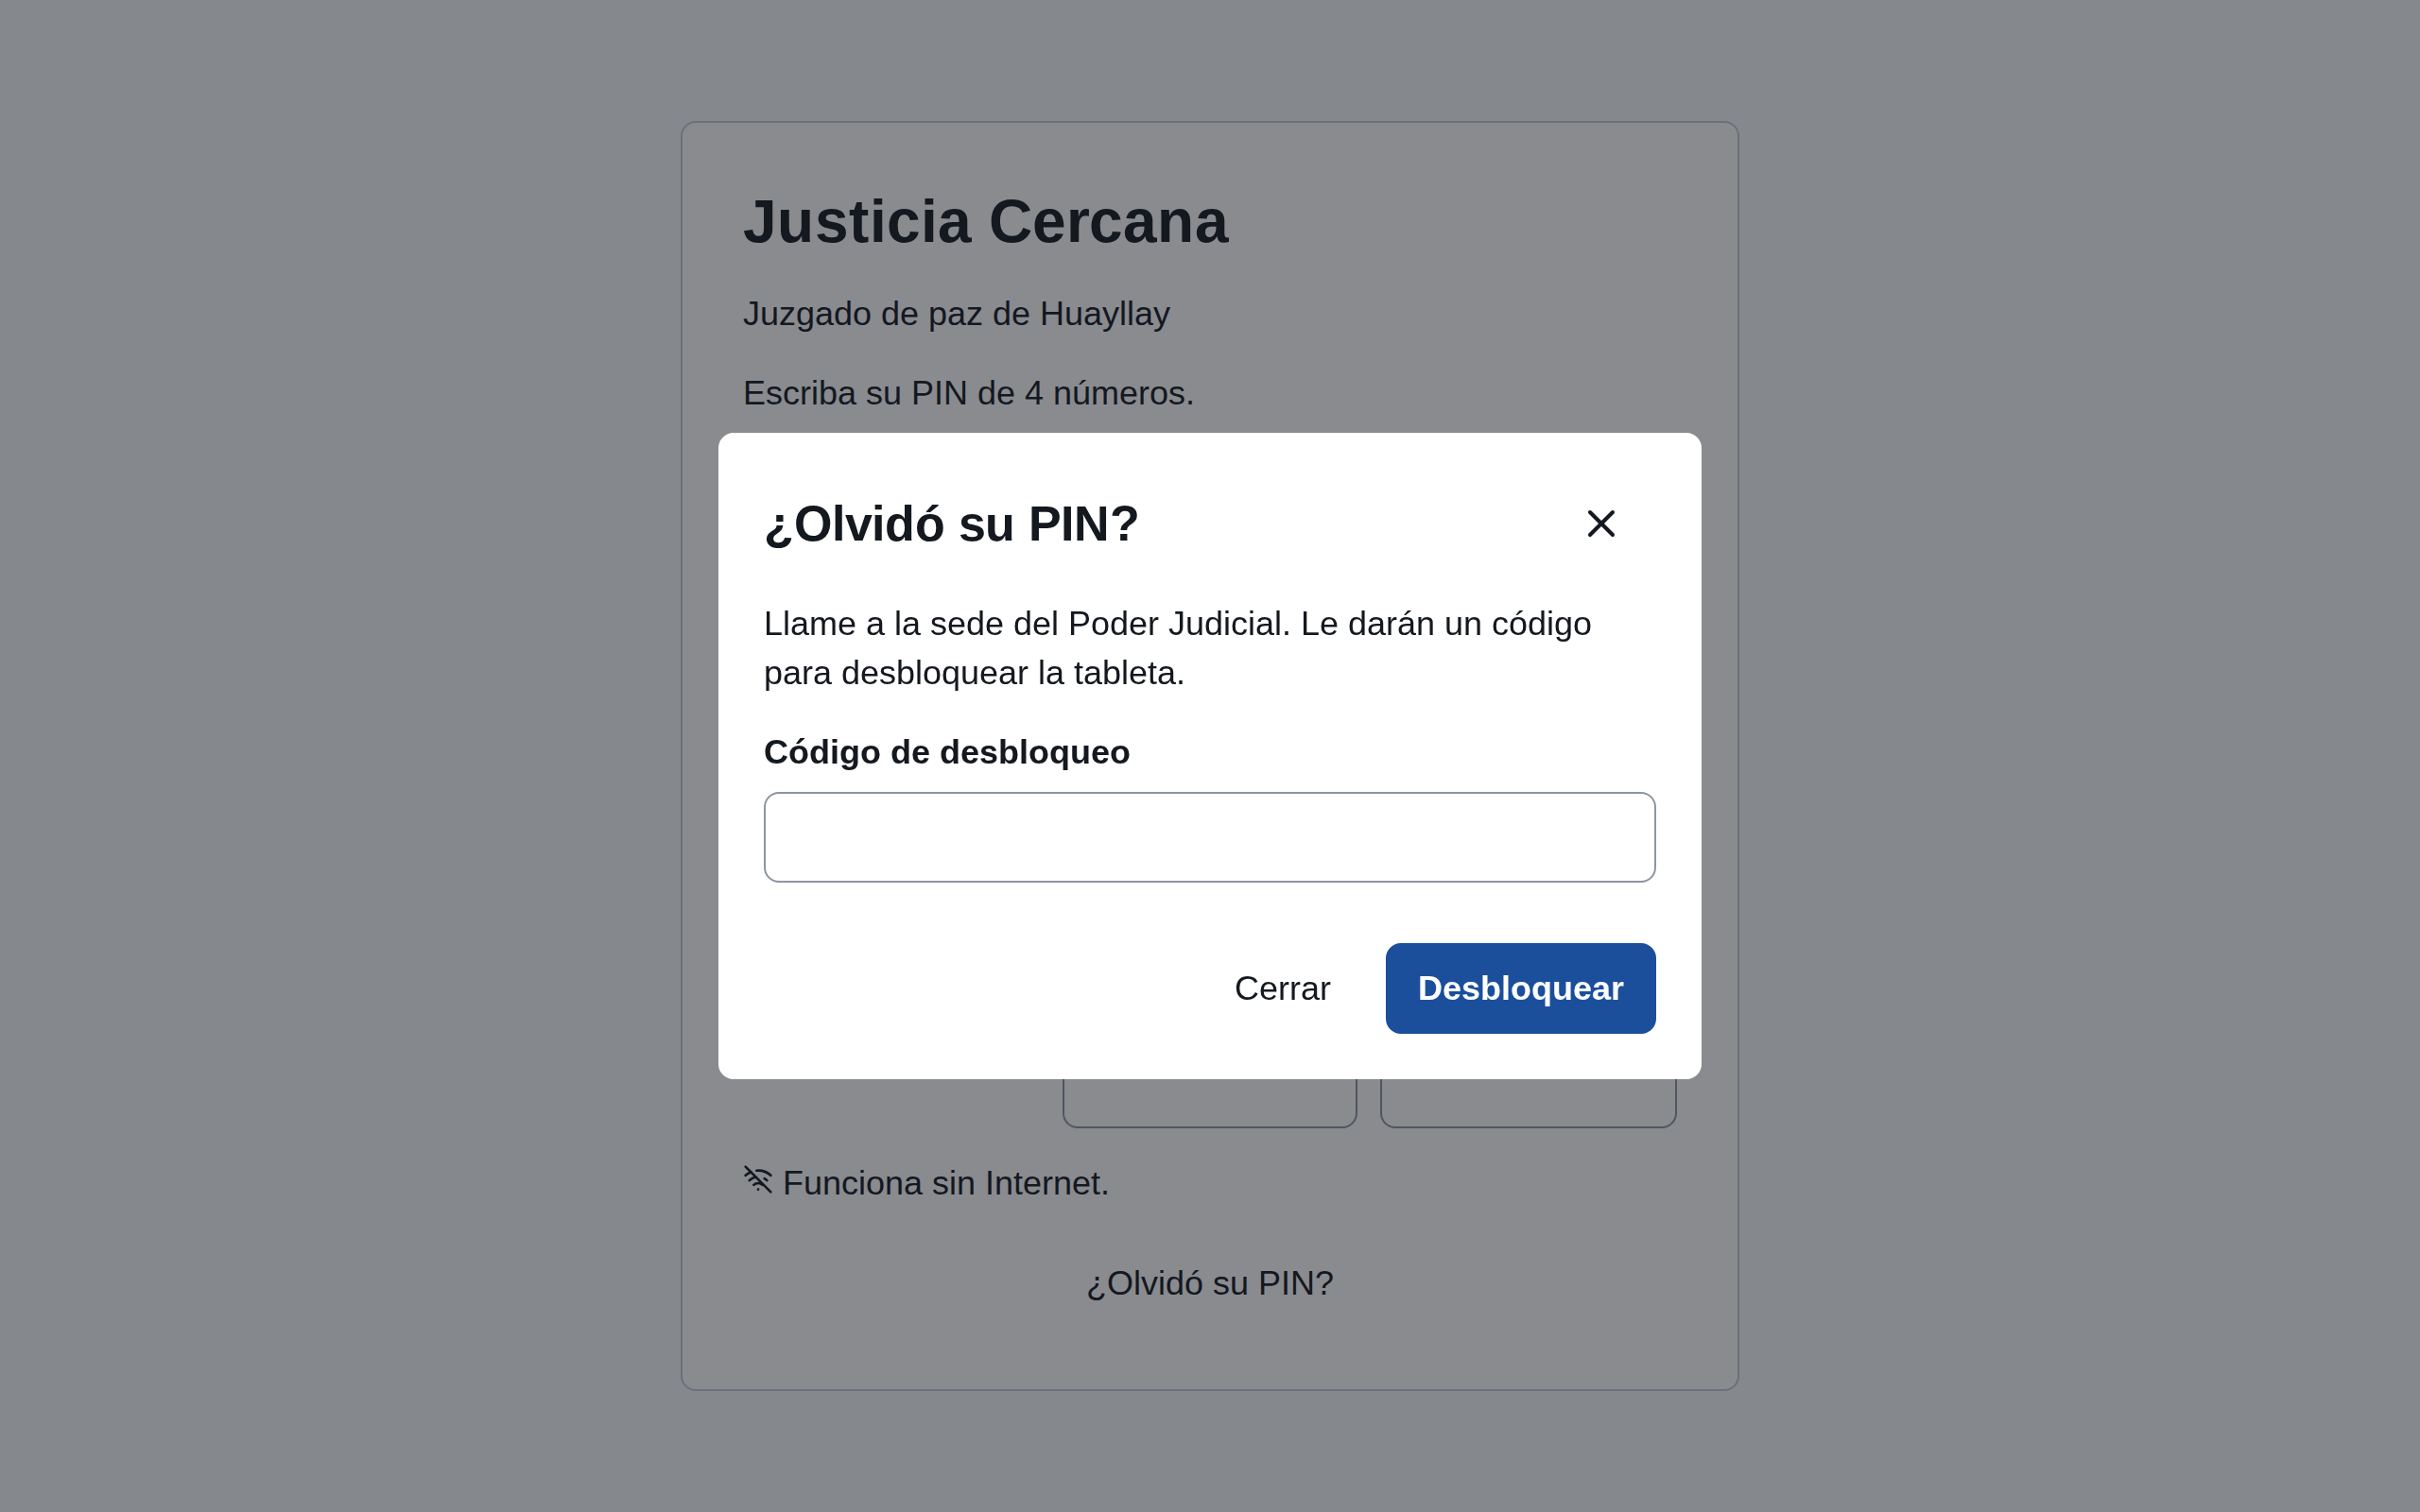
\includegraphics[width=0.86\linewidth]{capturas/P-00b_olvido-pin.png}
\caption{P-00 · Olvidó el PIN. Recuperación explicada en lenguaje cotidiano, sin bloqueo del trabajo}
\end{figure}
\begin{figure}[H]\centering
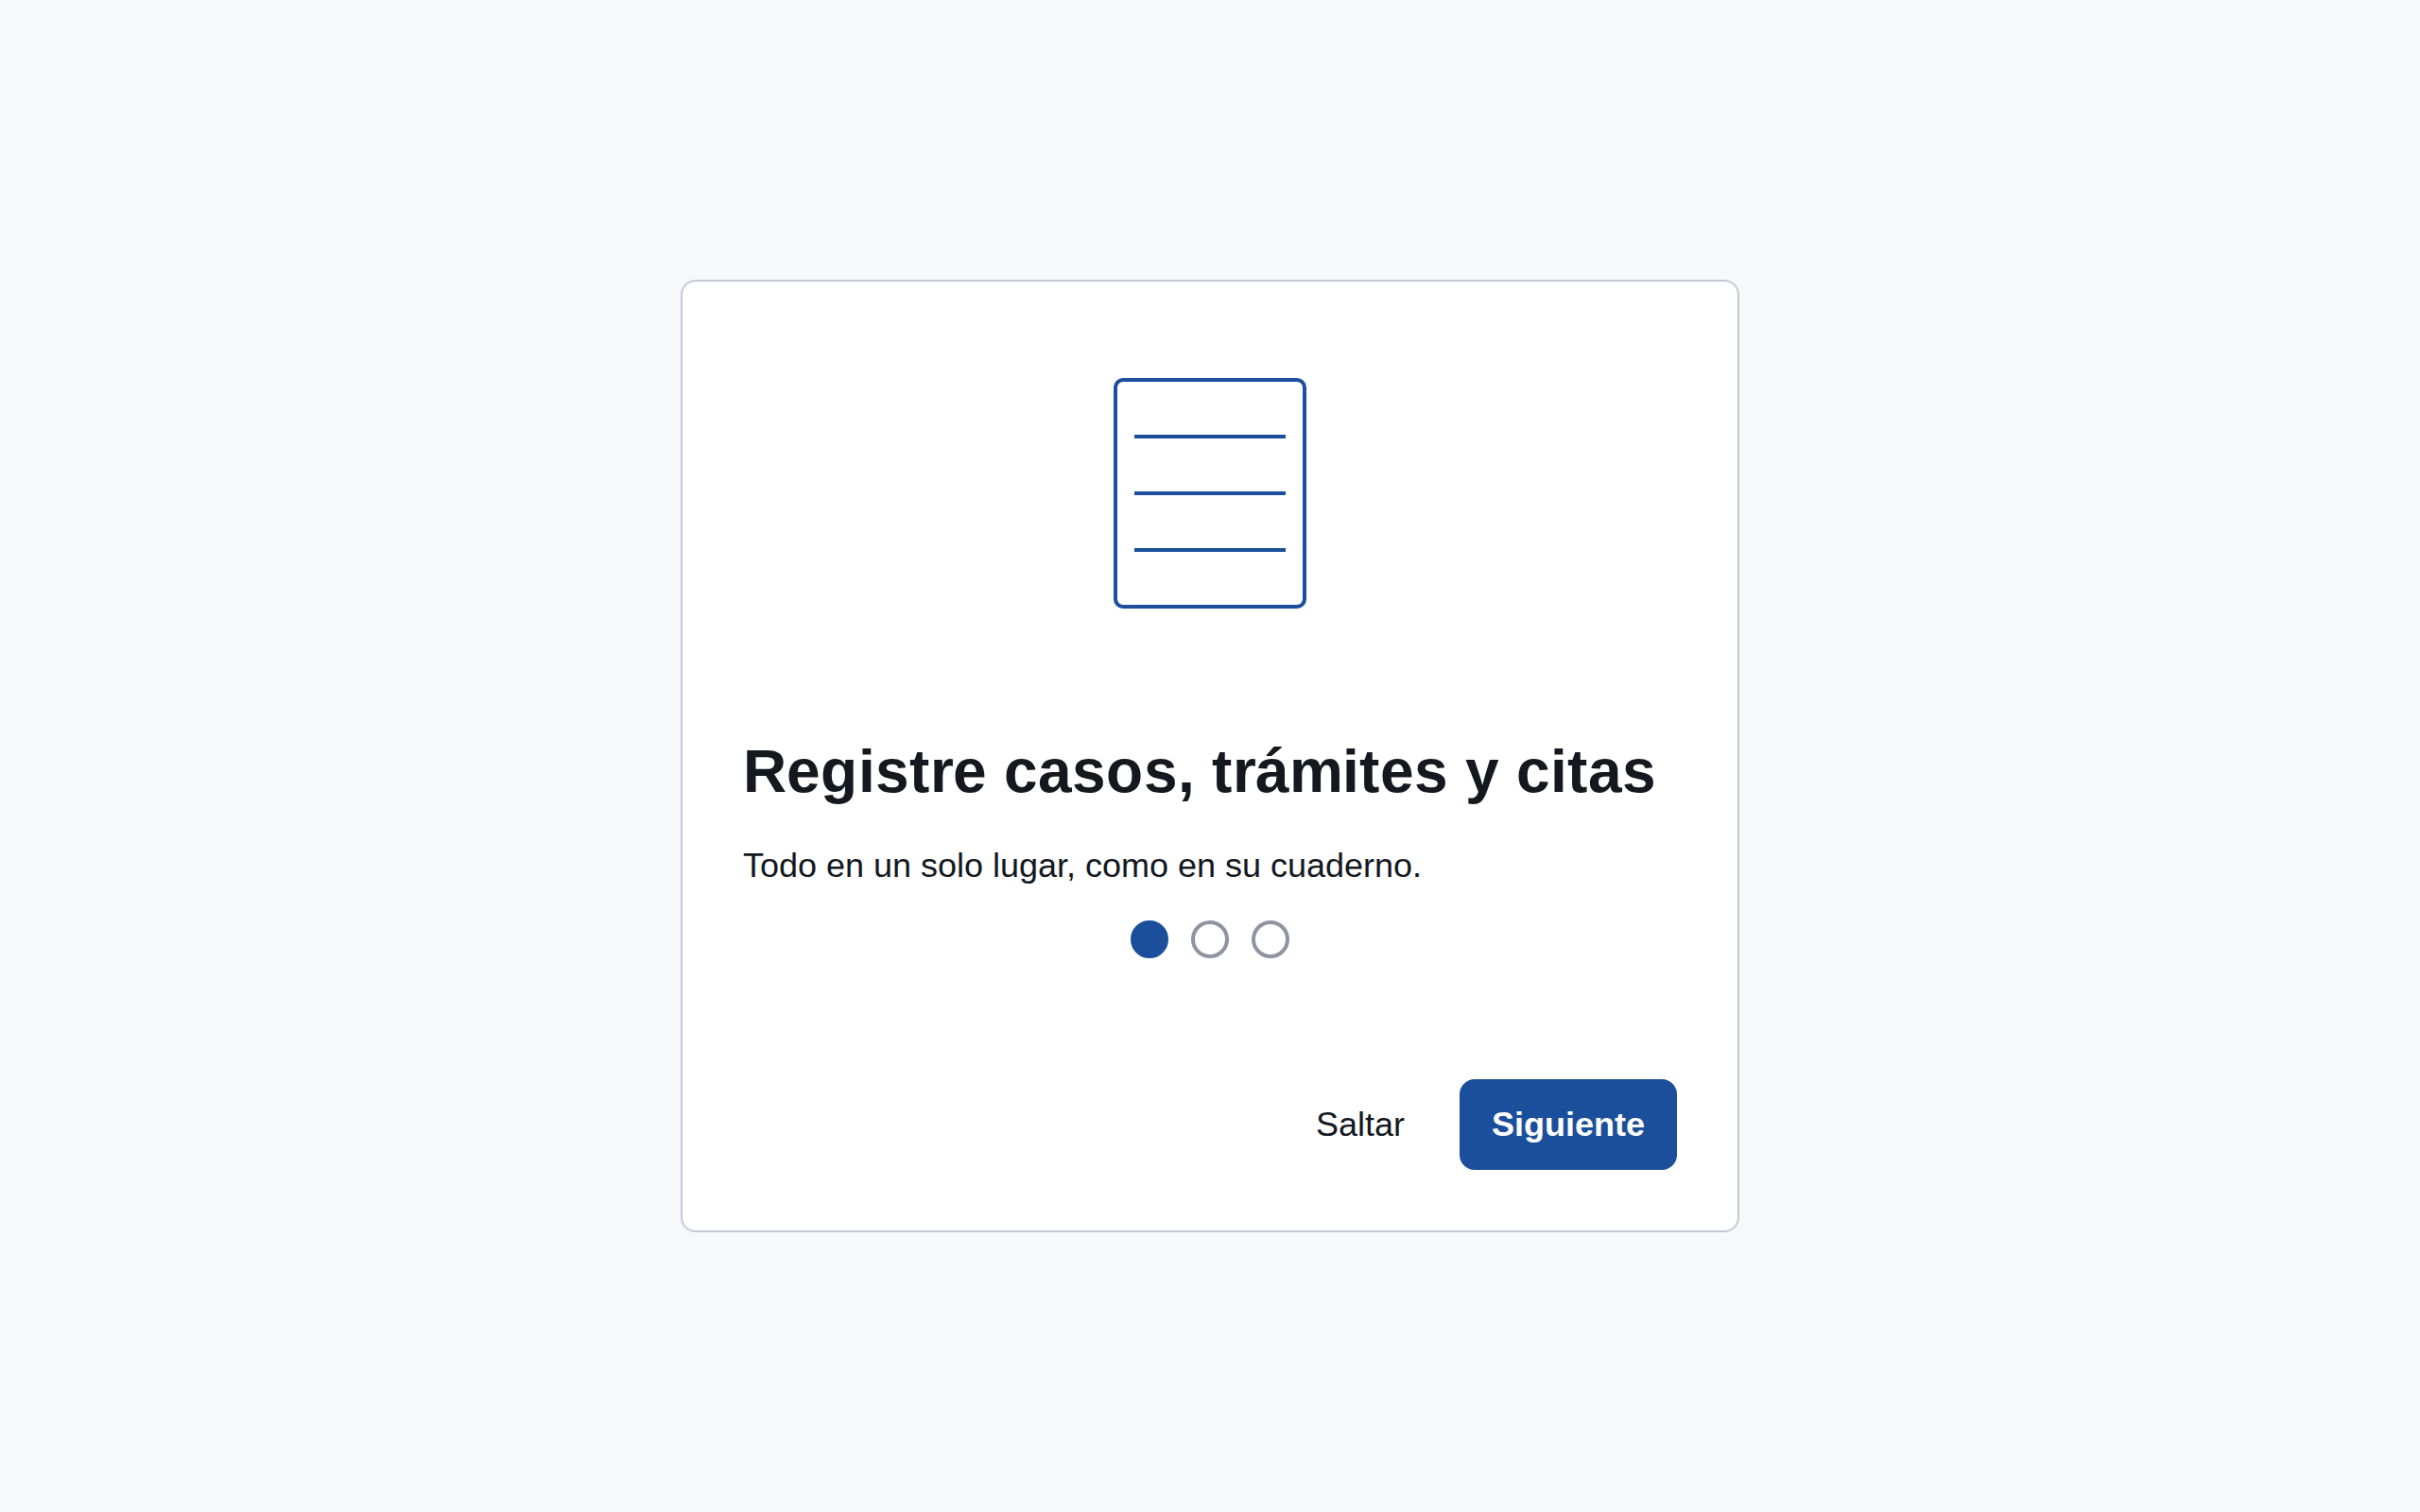
\includegraphics[width=0.86\linewidth]{capturas/P-00c_intro-1.png}
\caption{P-00b · Introducción 1 de 3. Introducción de tres pantallas con botón Saltar visible}
\end{figure}
\begin{figure}[H]\centering
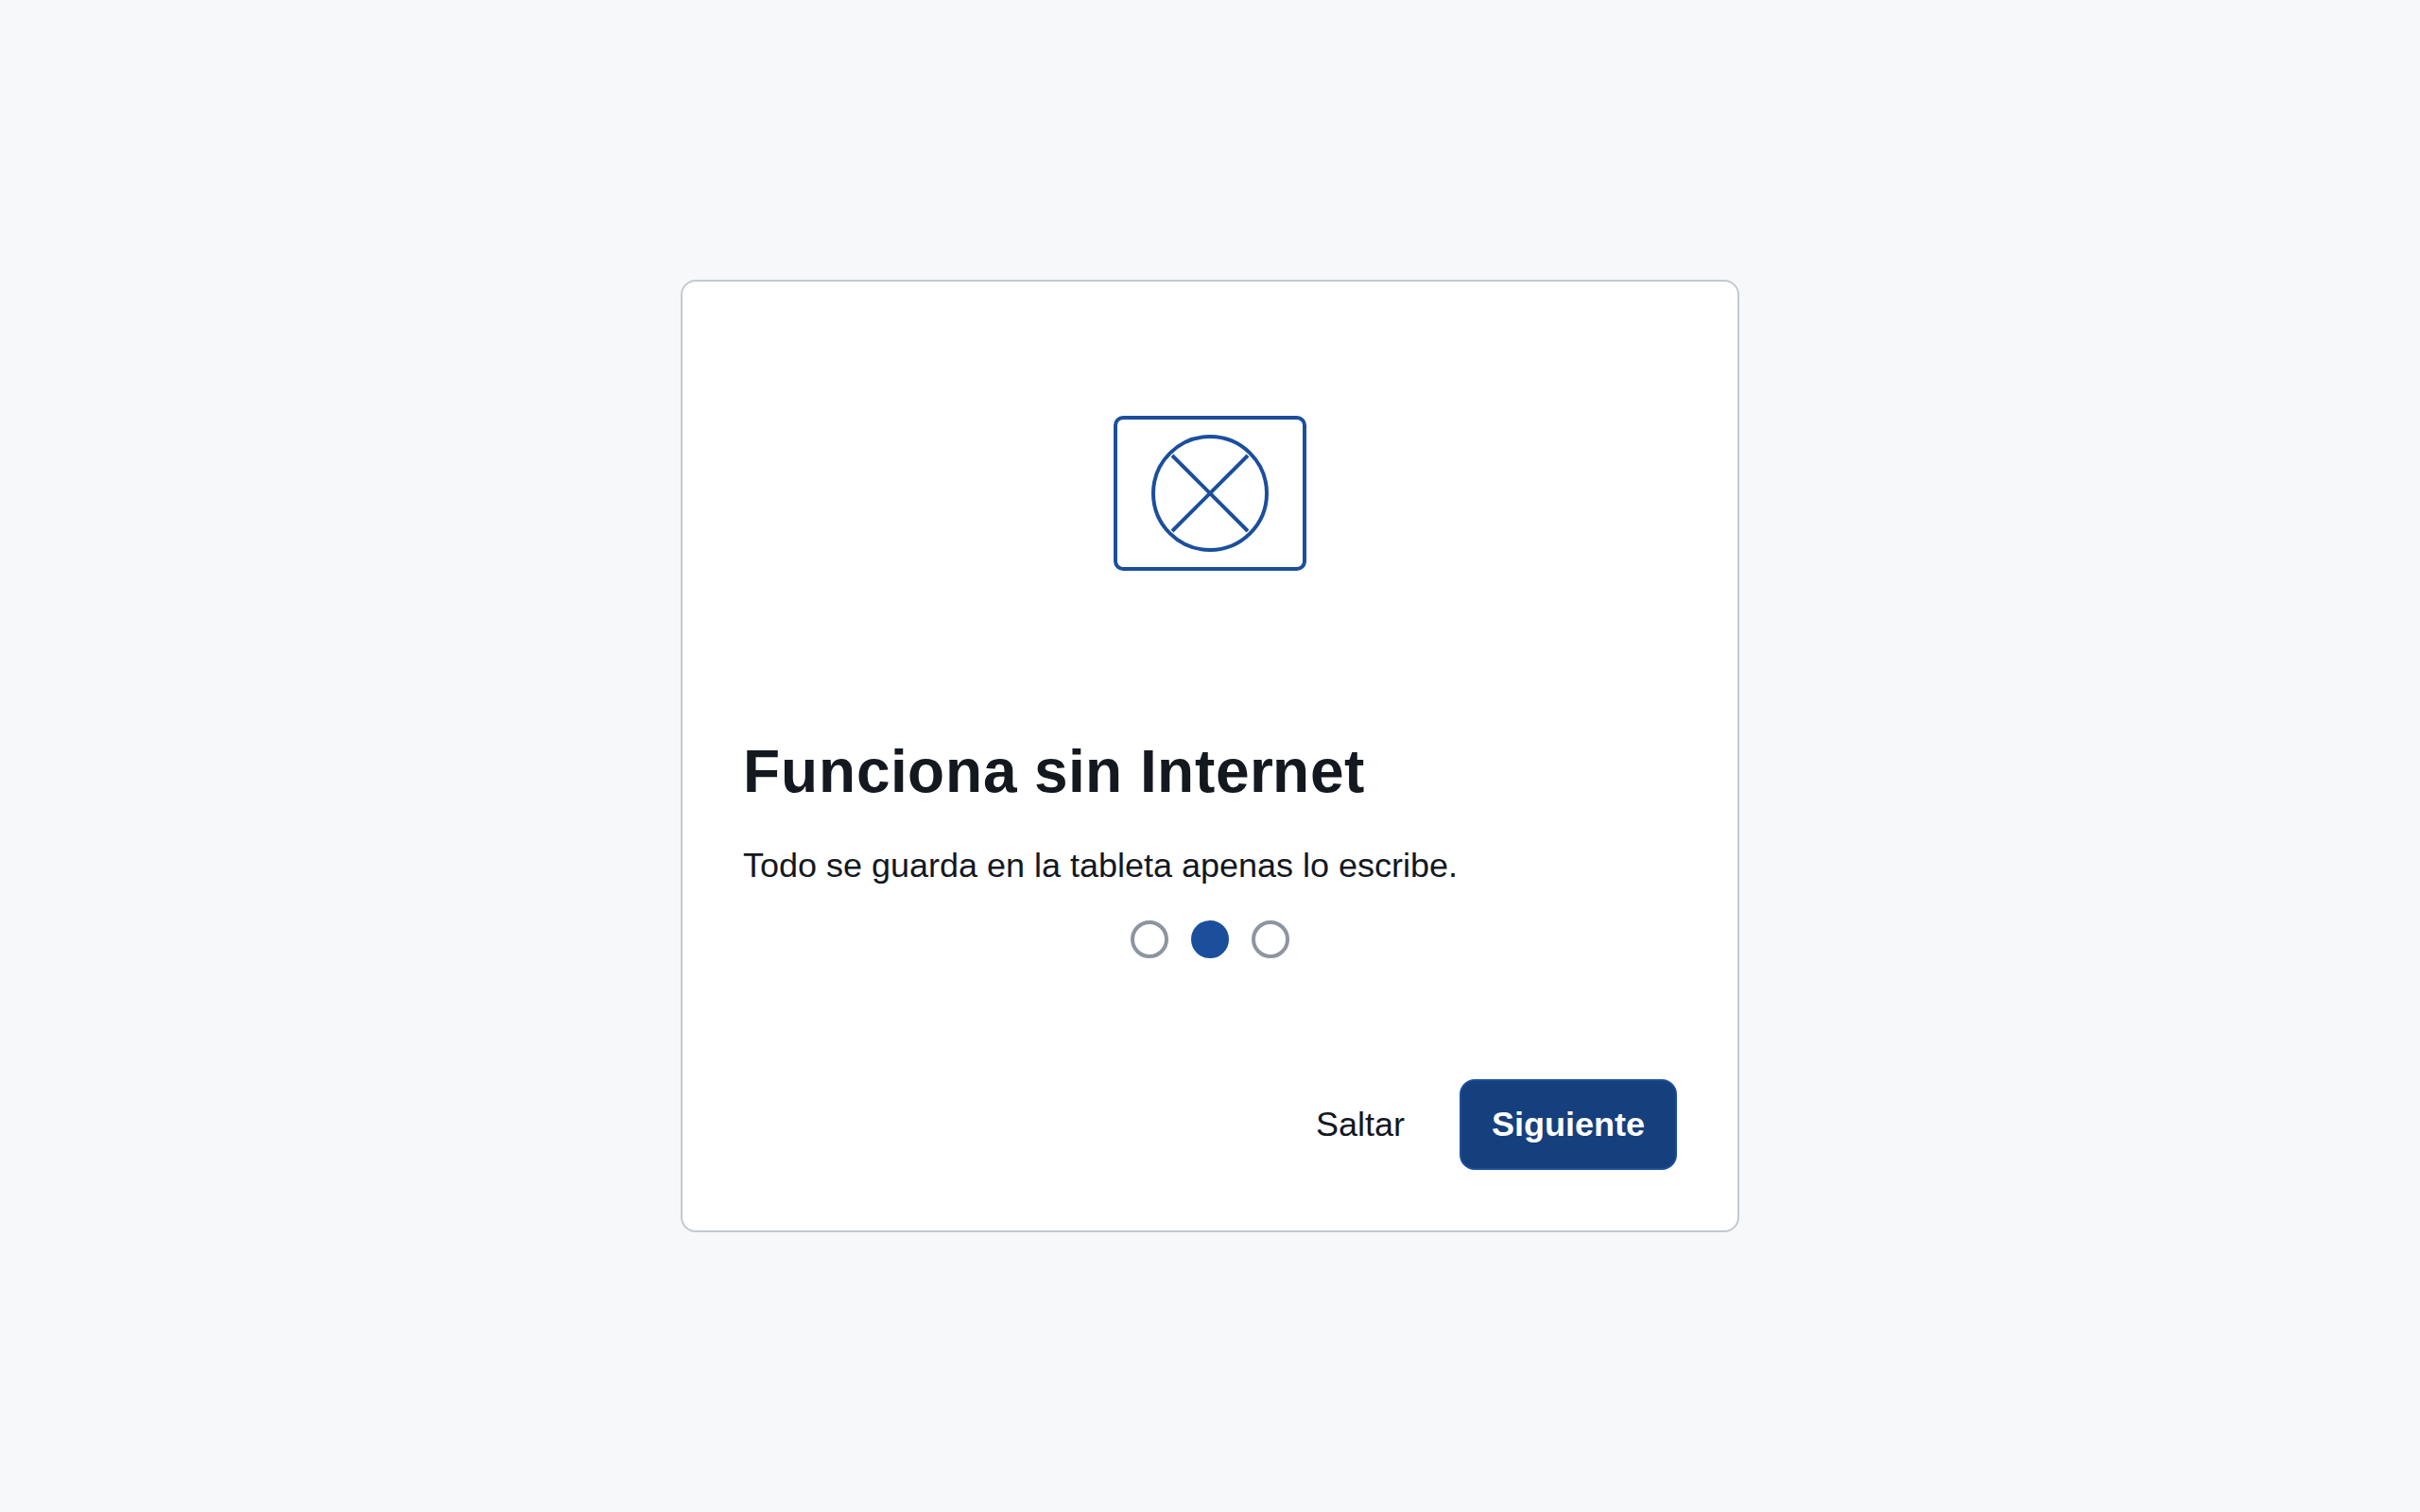
\includegraphics[width=0.86\linewidth]{capturas/P-00d_intro-2.png}
\caption{P-00b · Introducción 2 de 3. Se explica el trabajo sin Internet antes de usar la aplicación}
\end{figure}
\begin{figure}[H]\centering
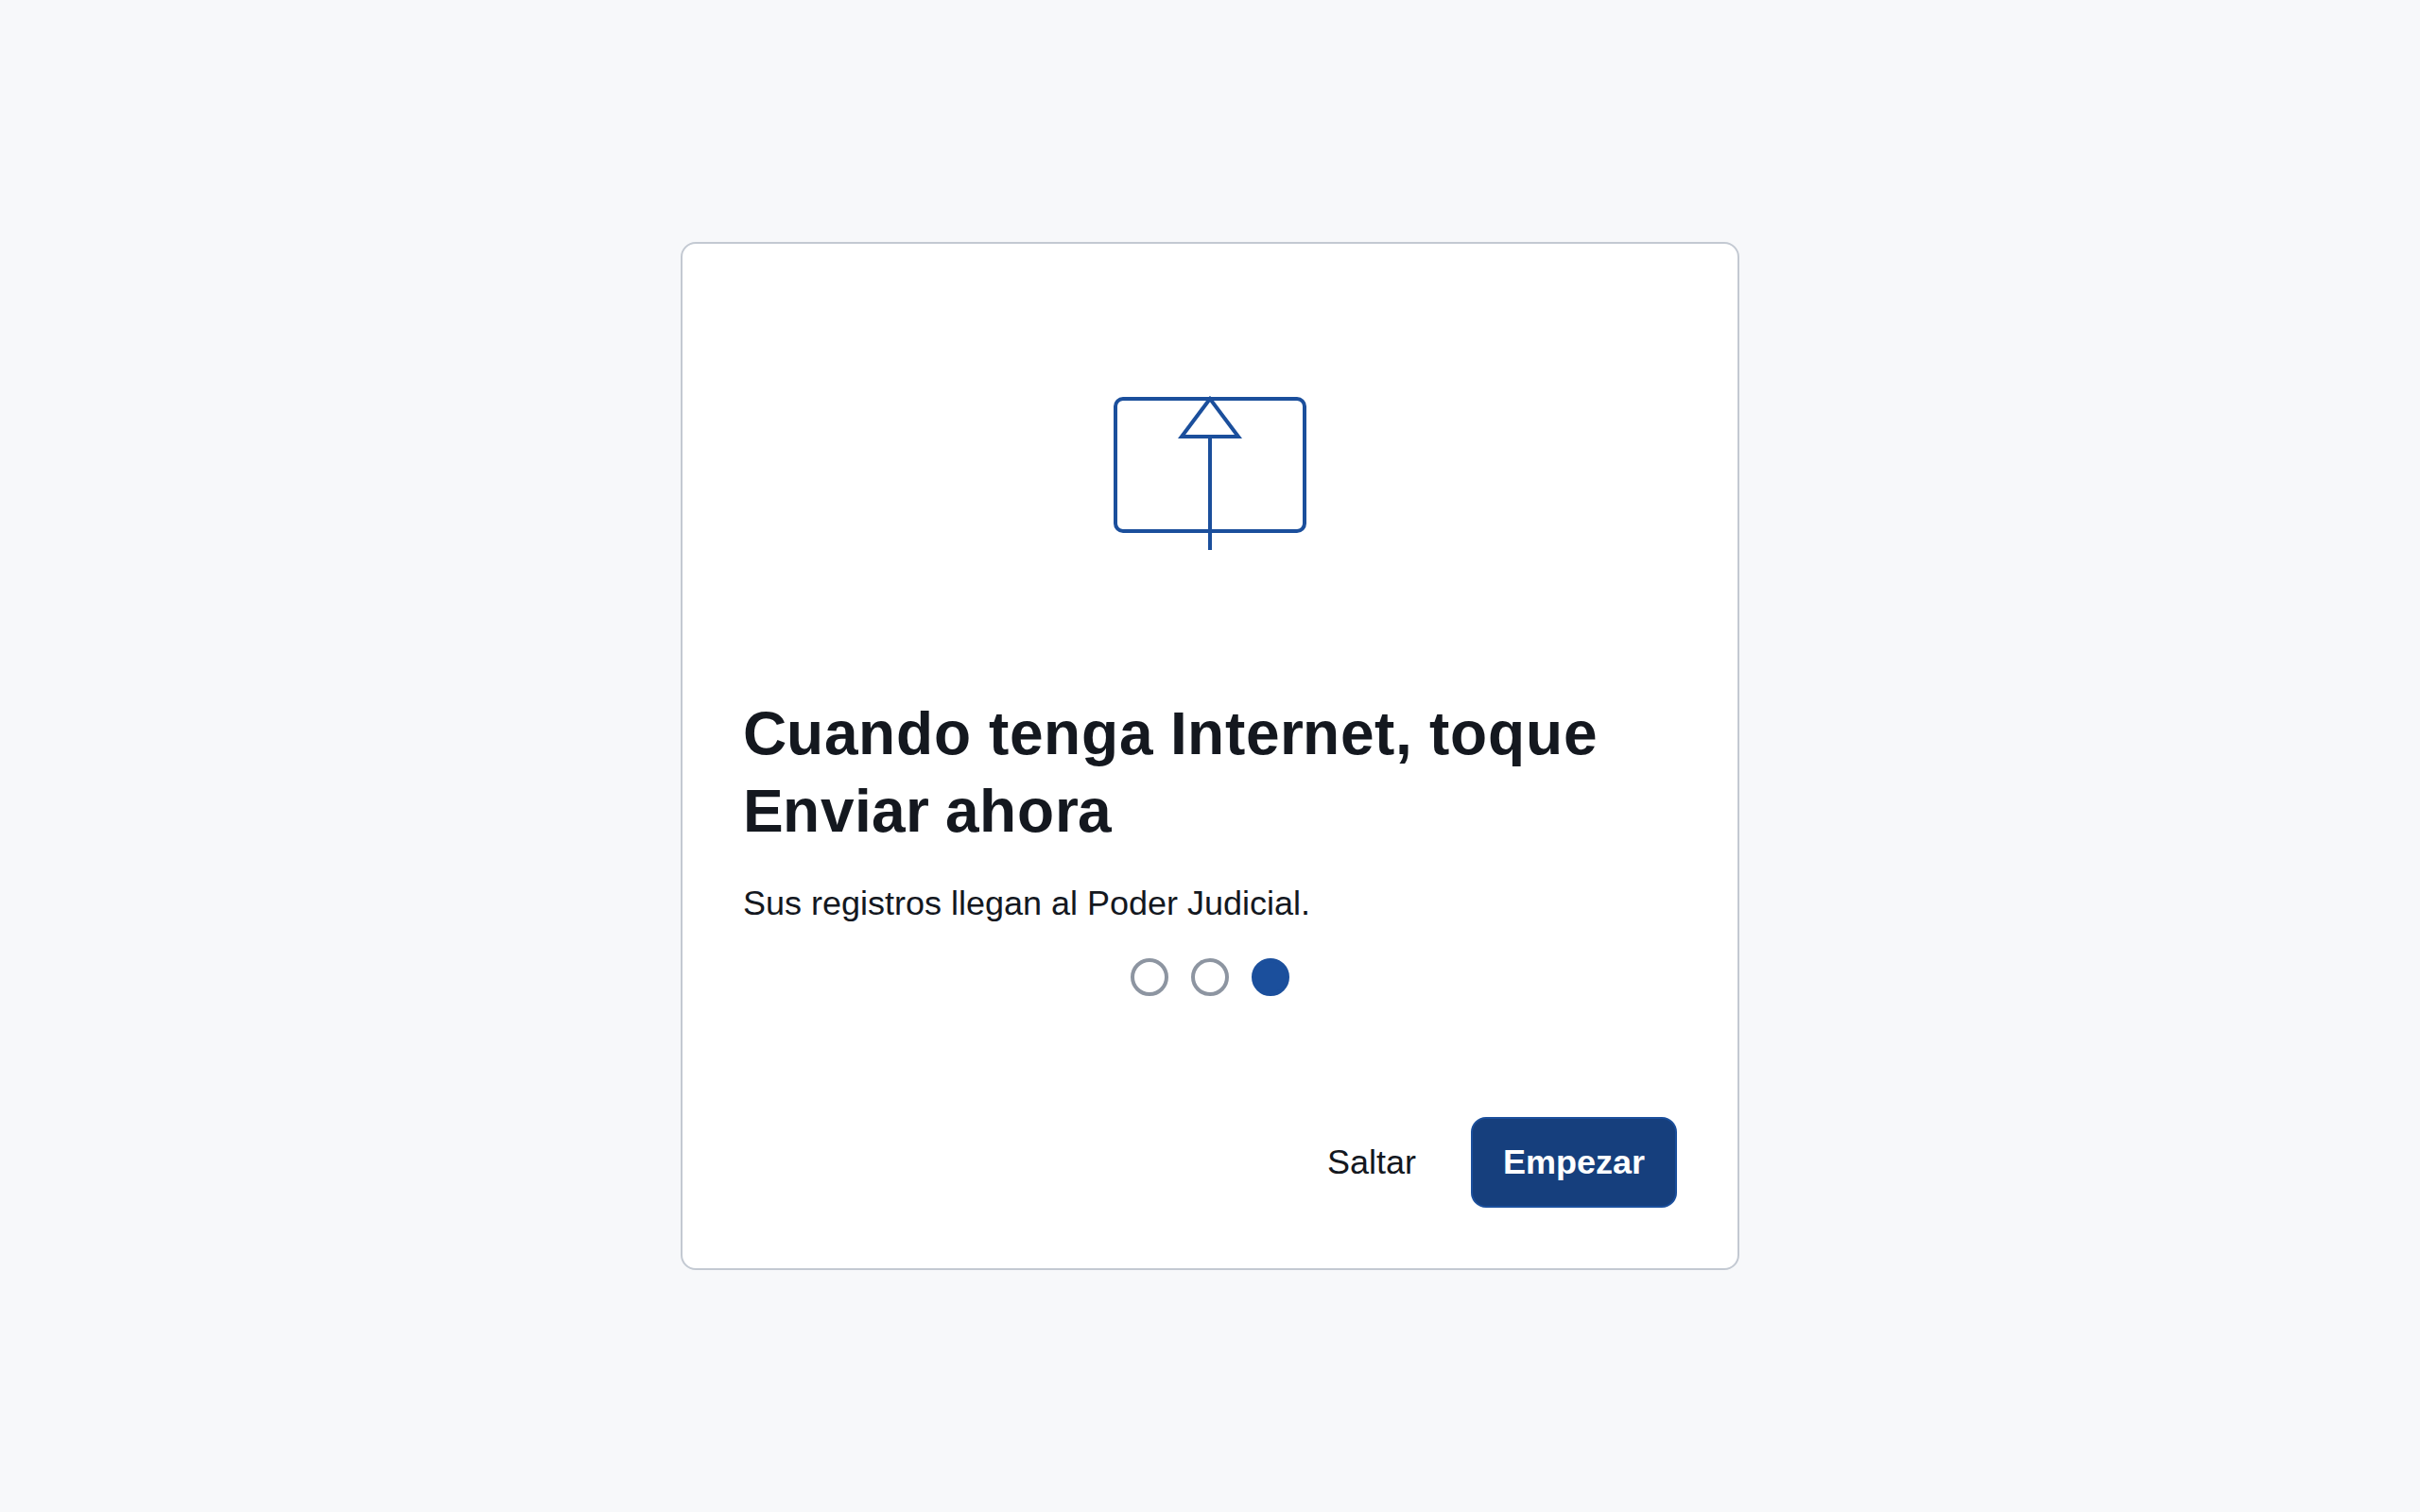
\includegraphics[width=0.86\linewidth]{capturas/P-00e_intro-3.png}
\caption{P-00b · Introducción 3 de 3. Se enseña el botón Enviar ahora antes de necesitarlo}
\end{figure}
\begin{figure}[H]\centering
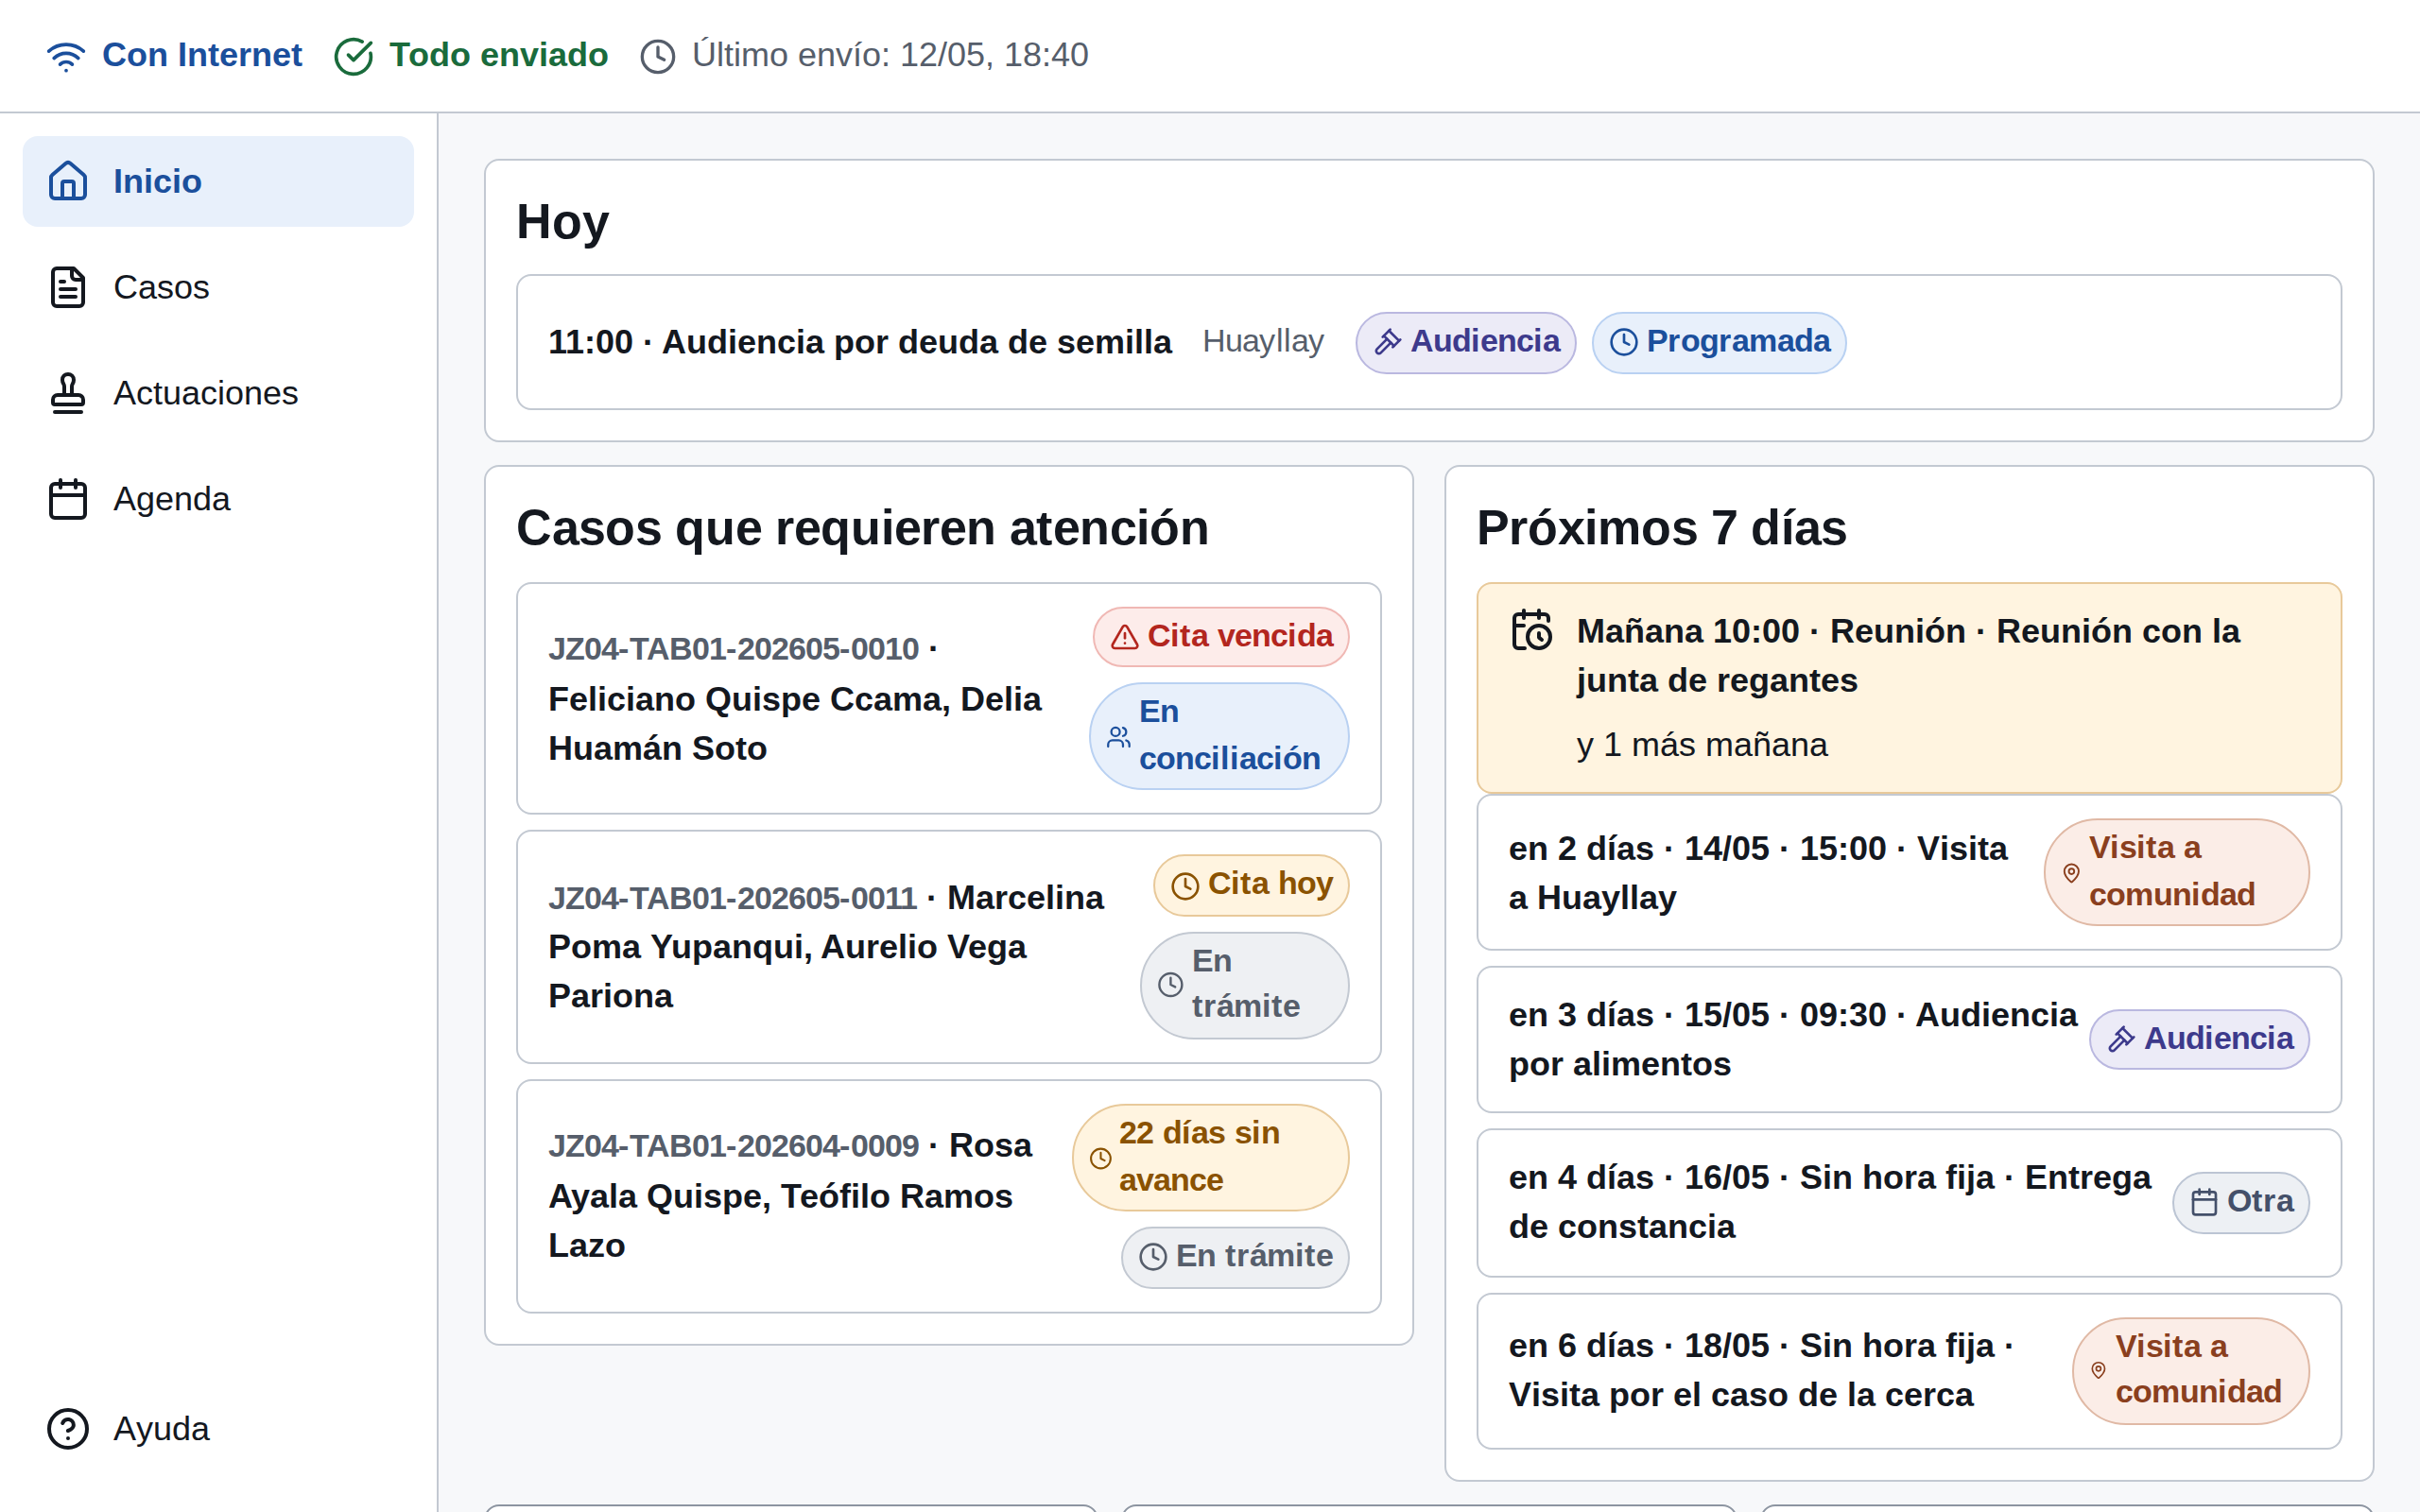
\includegraphics[width=0.86\linewidth]{capturas/P-01_inicio.png}
\caption{P-01 · Estado normal. Inicio con hoy, casos que requieren atención y próximos 7 días}
\end{figure}
\begin{figure}[H]\centering
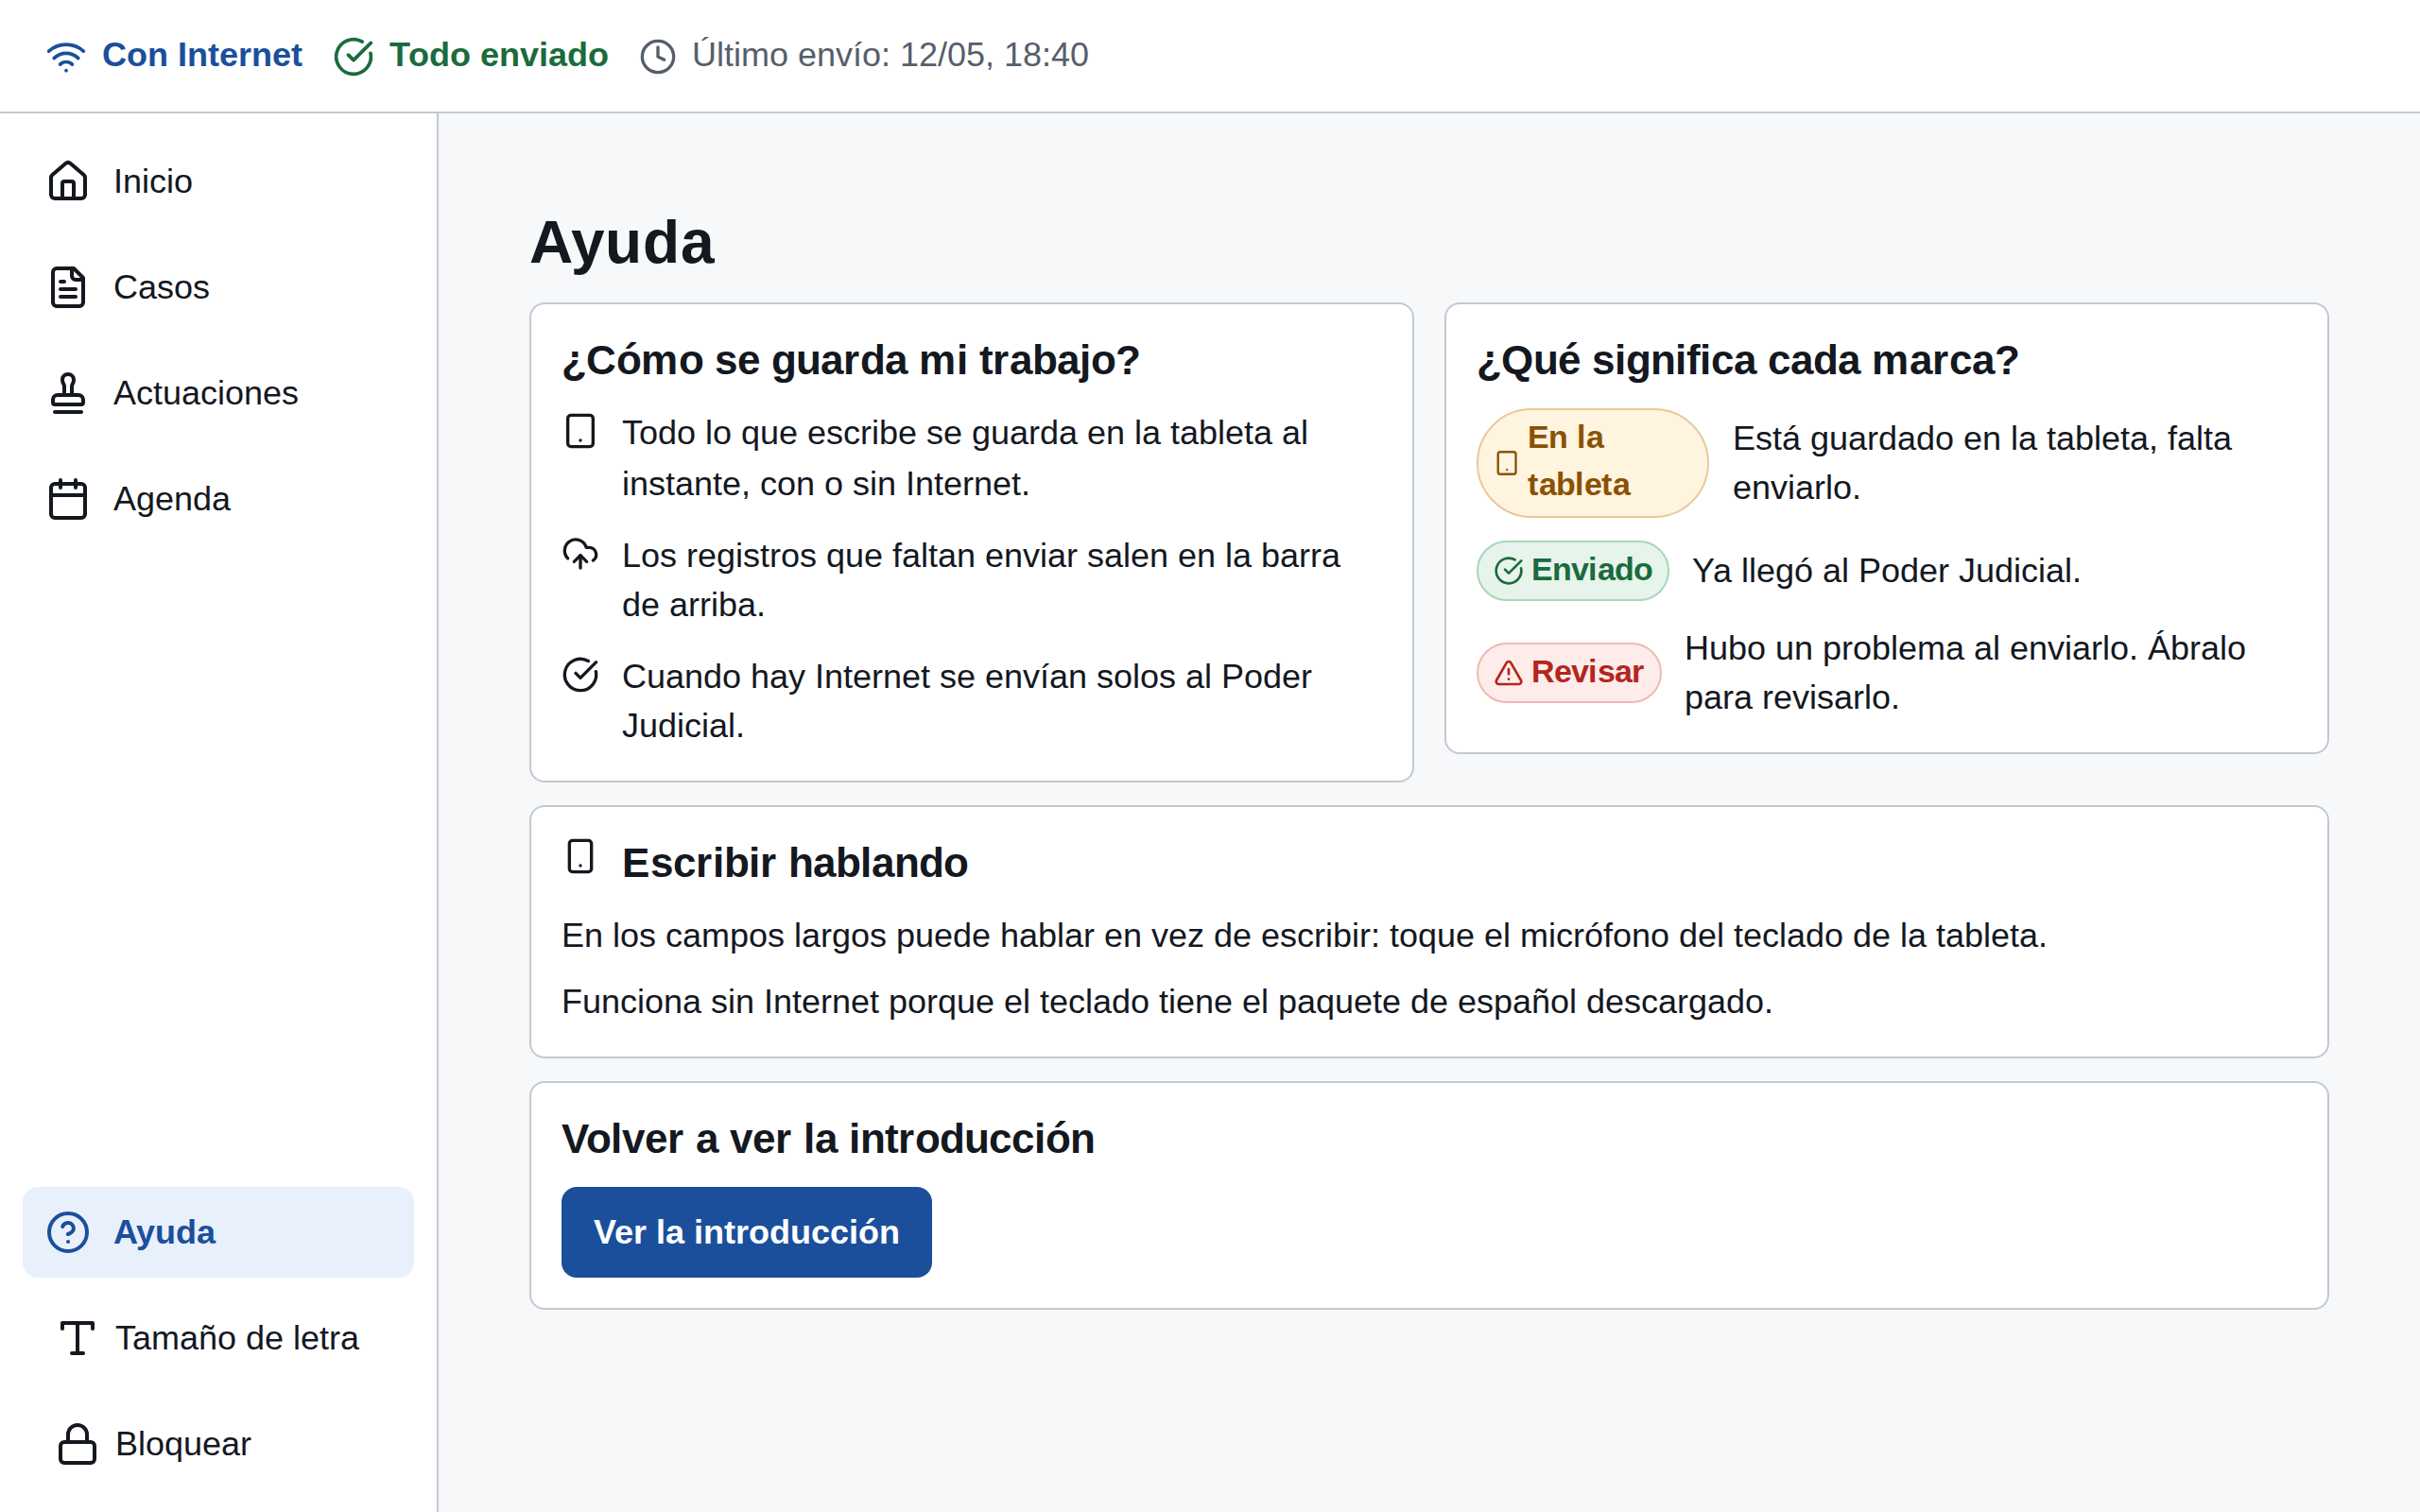
\includegraphics[width=0.86\linewidth]{capturas/Ayuda_ayuda.png}
\caption{Ayuda · Estado normal. Ayuda con el significado de cada marca y el dictado del teclado}
\end{figure}


\section{Módulo 1 · Casos}

\subsection{Tareas que permite}

Registrar un caso con varias partes, buscarlo por nombre o DNI, filtrarlo por comunidad, estado y fechas, abrir su detalle, registrar avances y editar sus datos.

\subsection{Campos del caso}

\begin{center}
\small
\begin{tabular}{@{}p{2.6cm}p{2.4cm}p{3.0cm}p{6.4cm}@{}}
\toprule
\textbf{Campo} & \textbf{Obligatoriedad} & \textbf{Control} & \textbf{Validación y mensaje} \\
\midrule
Código & Automático & Solo lectura & Se genera en la tableta y es definitivo \\
Fecha de registro & Automática, editable & Fecha, hoy prellenado & «La fecha no puede ser posterior a hoy.» \\
Tipo de conflicto & Obligatorio & Botones grandes & «Elija de qué trata el problema.» \\
Descripción & Obligatorio & Texto amplio & «Cuente brevemente qué pasó.» \\
Estado & Obligatorio & Botones segmentados & Concluido exige acuerdo o resultado \\
Observaciones & Opcional & Texto amplio & --- \\
\bottomrule
\end{tabular}
\end{center}

La fecha de registro es editable porque el reloj de una tableta sin conexión puede estar desfasado.

\subsection{Campos de cada parte}

\begin{center}
\small
\begin{tabular}{@{}p{3.0cm}p{2.6cm}p{8.6cm}@{}}
\toprule
\textbf{Campo} & \textbf{Obligatoriedad} & \textbf{Validación y mensaje} \\
\midrule
Nombres y apellidos & Obligatorio & «Escriba el nombre y al menos un apellido.» \\
Tipo de documento & Opcional & DNI, carné de extranjería, otro, no tiene, no lo tiene a la mano \\
Número de documento & Condicional & «El DNI tiene 8 números. Revíselo o elija No lo tiene a la mano.» \\
Teléfono o contacto & Opcional & «El celular tiene 9 números.» Casilla «No tiene» \\
Comunidad o localidad & Obligatorio & «Indique la comunidad donde vive.» \\
Dirección o referencia & Opcional & --- \\
Rol & Obligatorio & «El caso necesita al menos una persona que lo solicite.» \\
\bottomrule
\end{tabular}
\end{center}

La comunidad es obligatoria y la dirección no, porque la comunidad se usa para buscar y para detectar personas repetidas, y casi siempre se conoce.

\subsection{Criterios de «requiere atención»}

Se calculan solos y se muestran escritos en la lista y en Inicio: \textbf{cita vencida} (la próxima fecha ya pasó y no hay un avance posterior), \textbf{cita hoy}, y \textbf{15 días o más sin avances} en estado En trámite o En conciliación.

\subsection{Por qué existe el estado «En conciliación»}

El enunciado pide los estados del caso sin fijarlos. Se agrega En conciliación porque la conciliación es la vía principal del juez de paz según la Ley 29824, y distingue los casos con diálogo entre partes en curso de los que solo están registrados. Sin ese estado, la jueza no podría separar los dos grupos al filtrar.

\begin{figure}[H]\centering
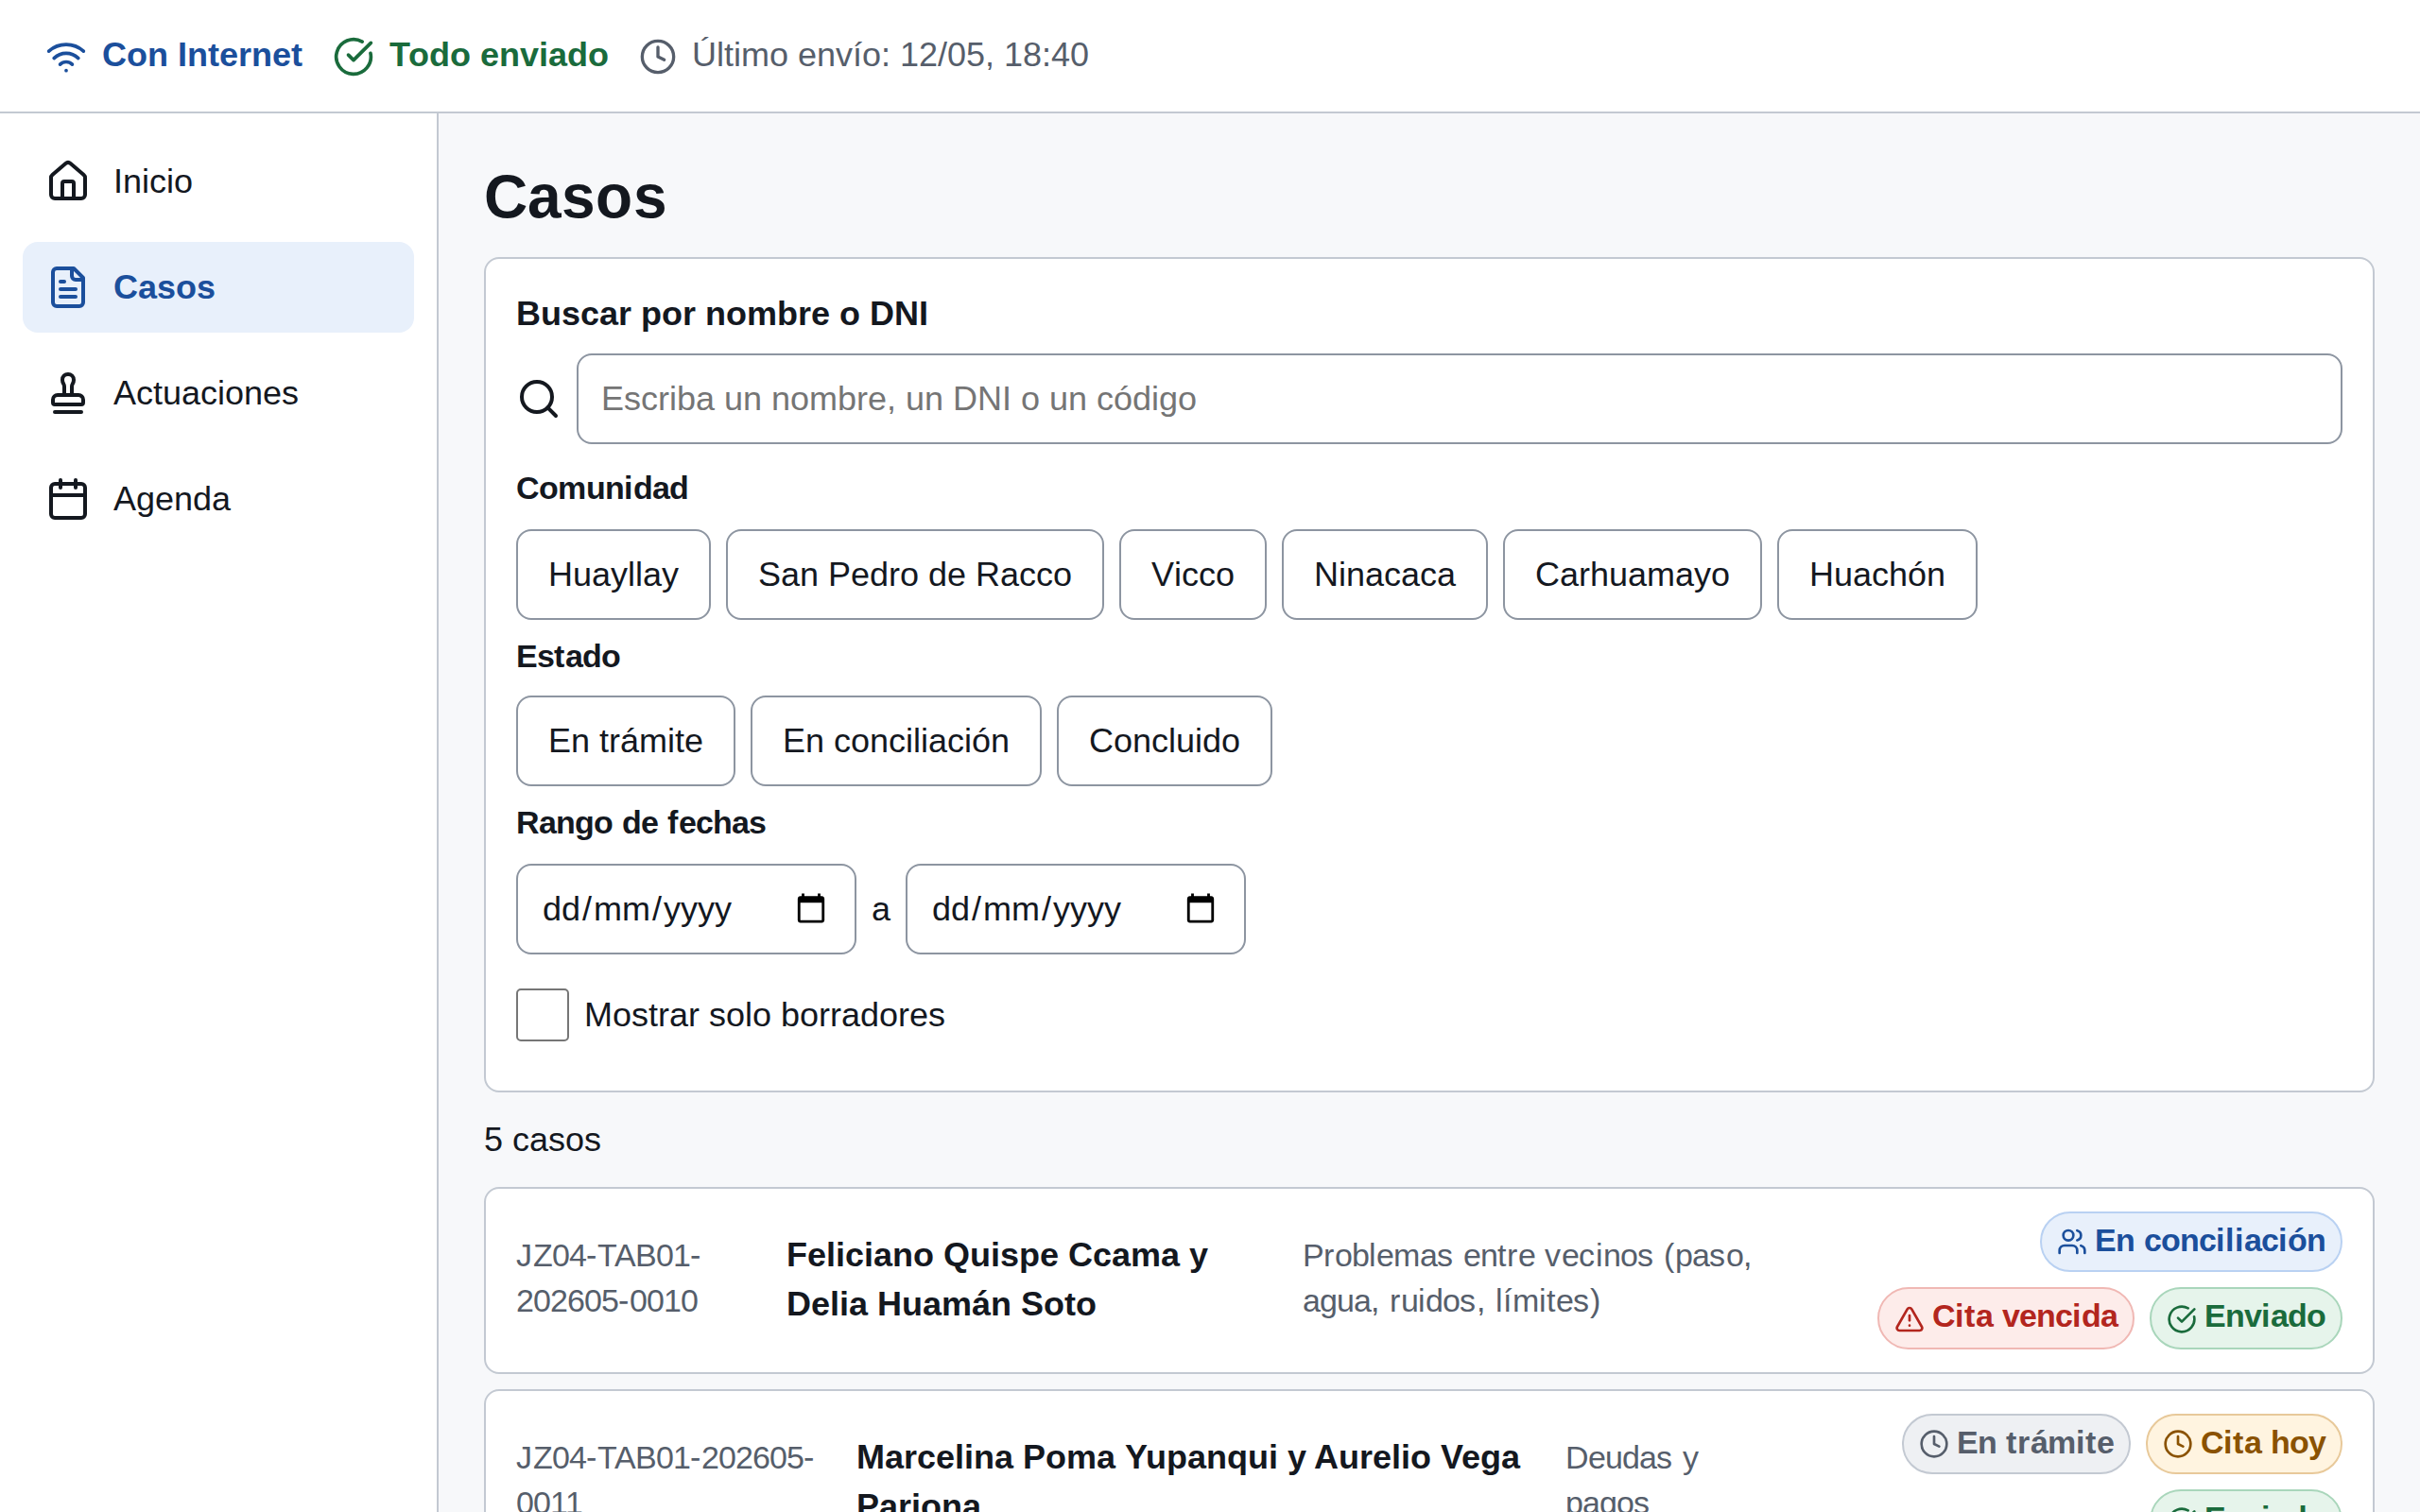
\includegraphics[width=0.86\linewidth]{capturas/P-02_casos-lista.png}
\caption{P-02 · Estado normal. Lista de casos con búsqueda, filtros y marcas por registro}
\end{figure}
\begin{figure}[H]\centering
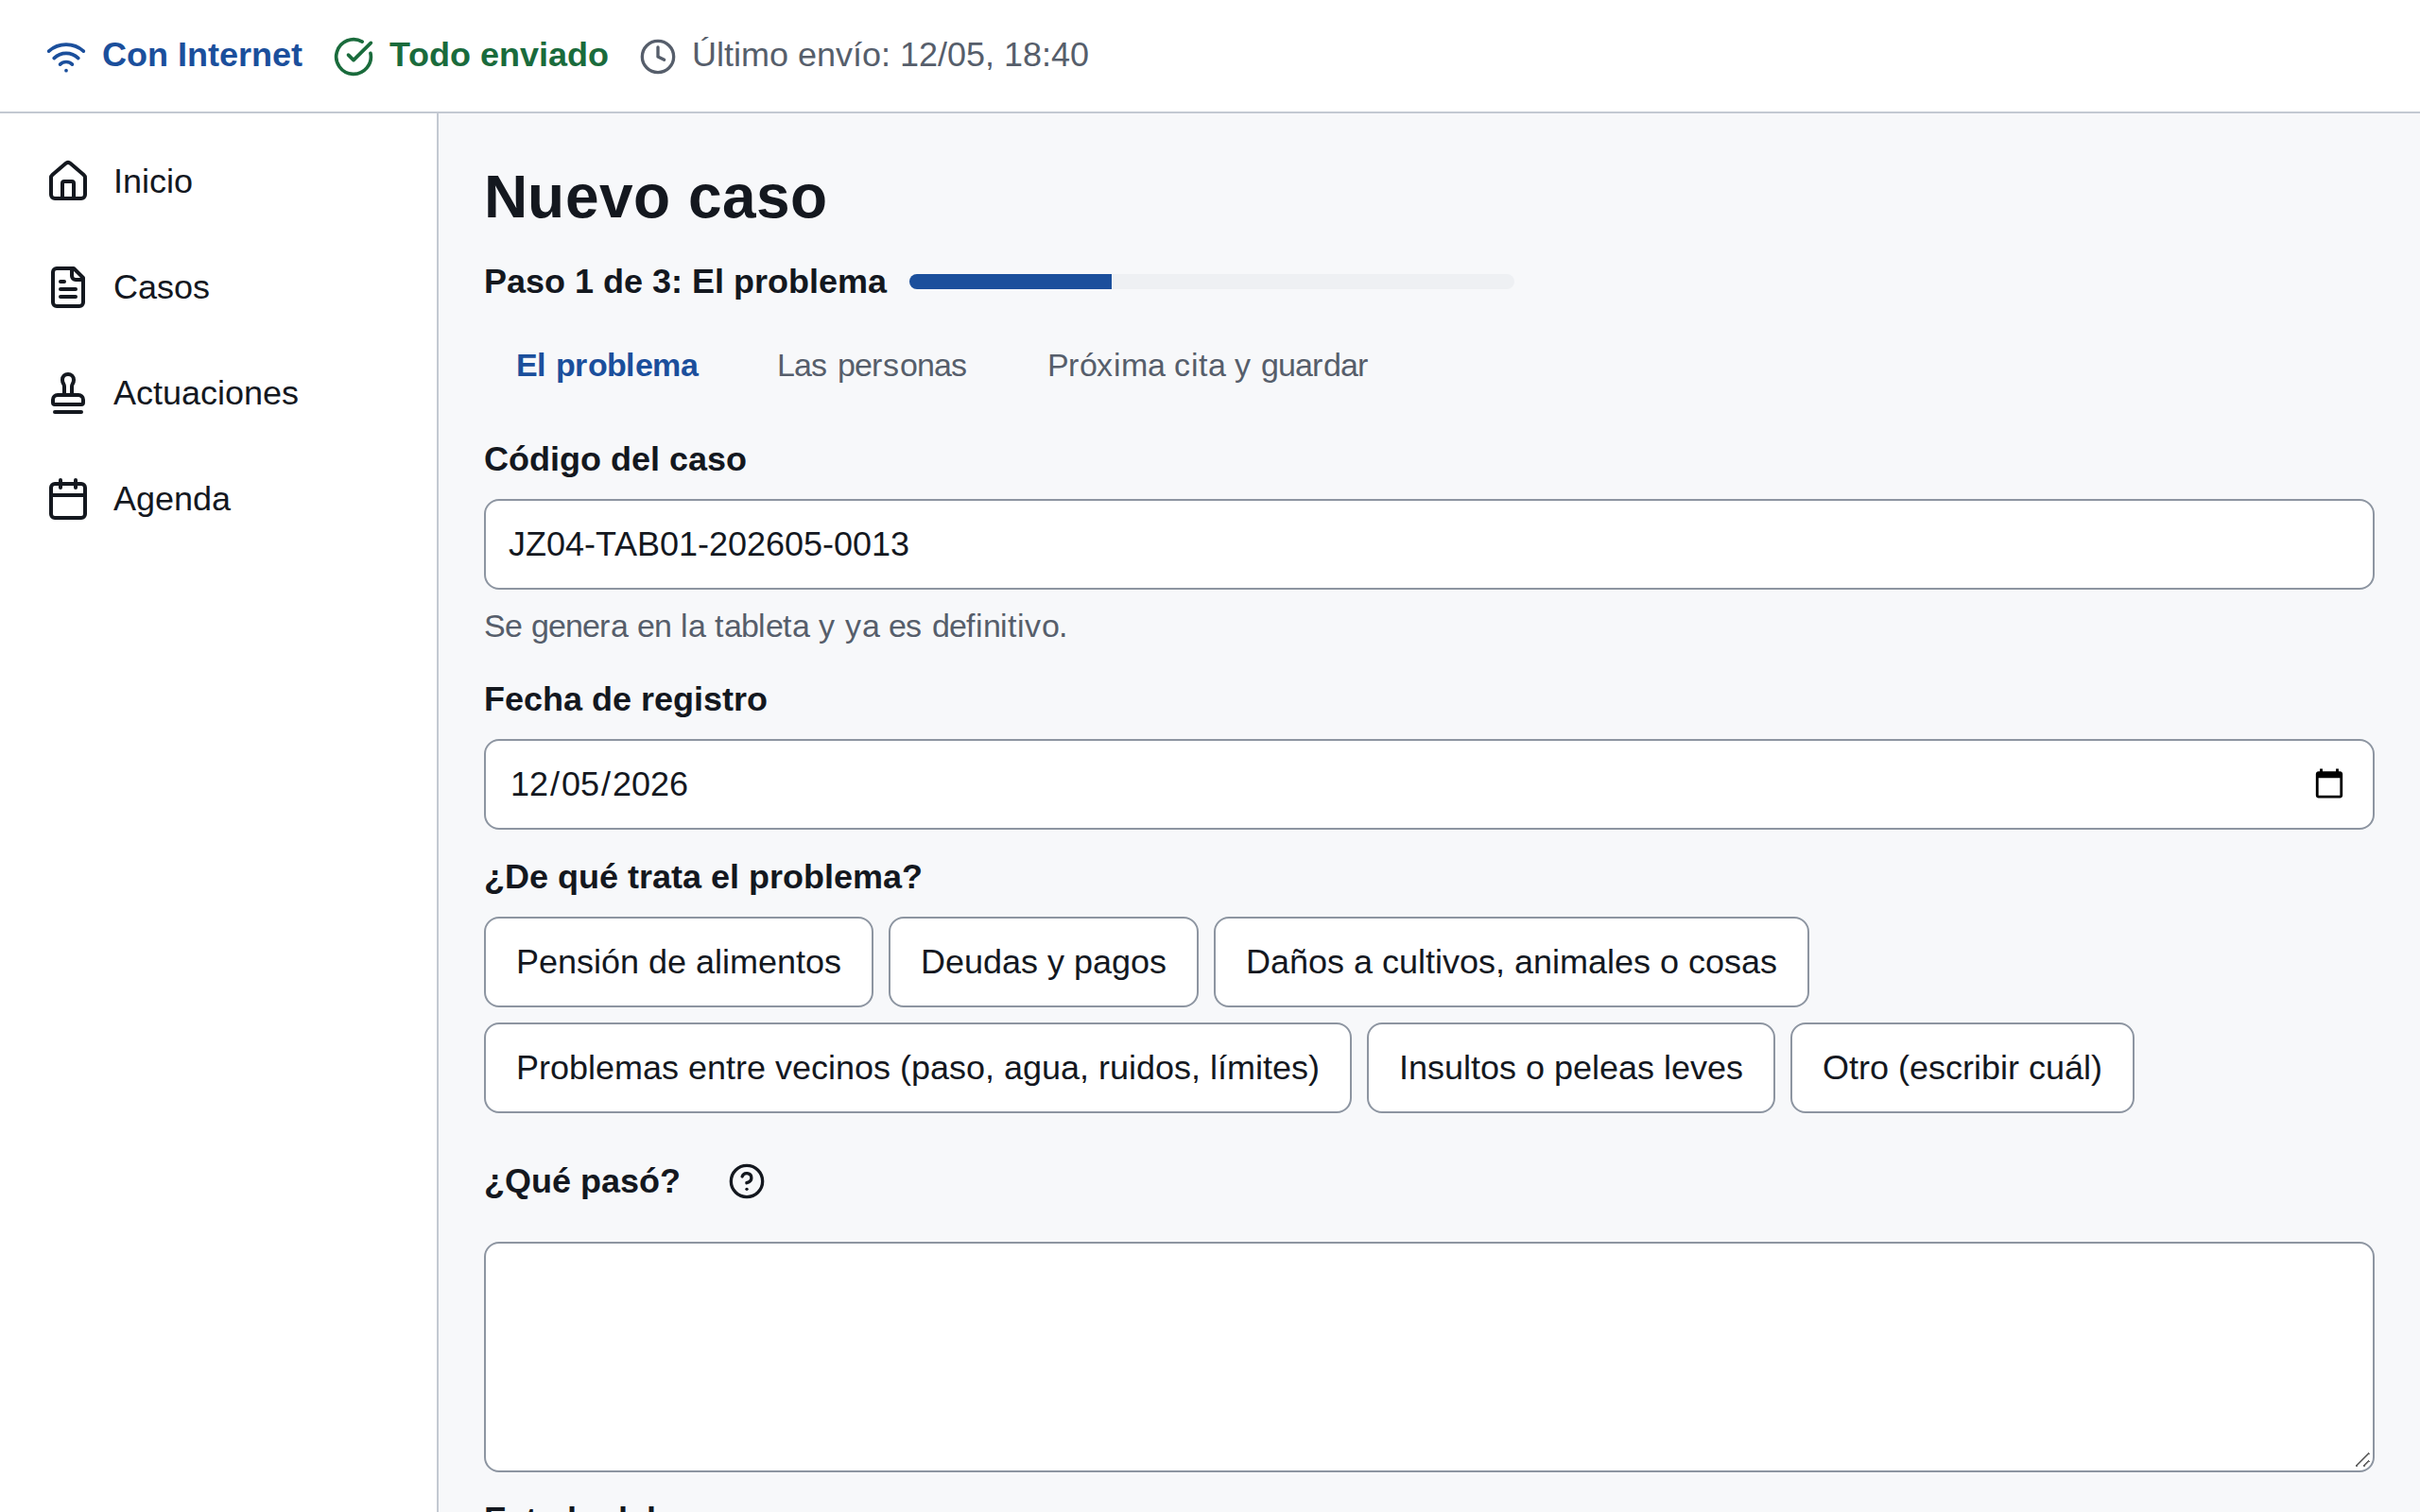
\includegraphics[width=0.86\linewidth]{capturas/P-03_caso-nuevo.png}
\caption{P-03 · Estado normal. Formulario de caso en 3 pasos, paso 1}
\end{figure}
\begin{figure}[H]\centering
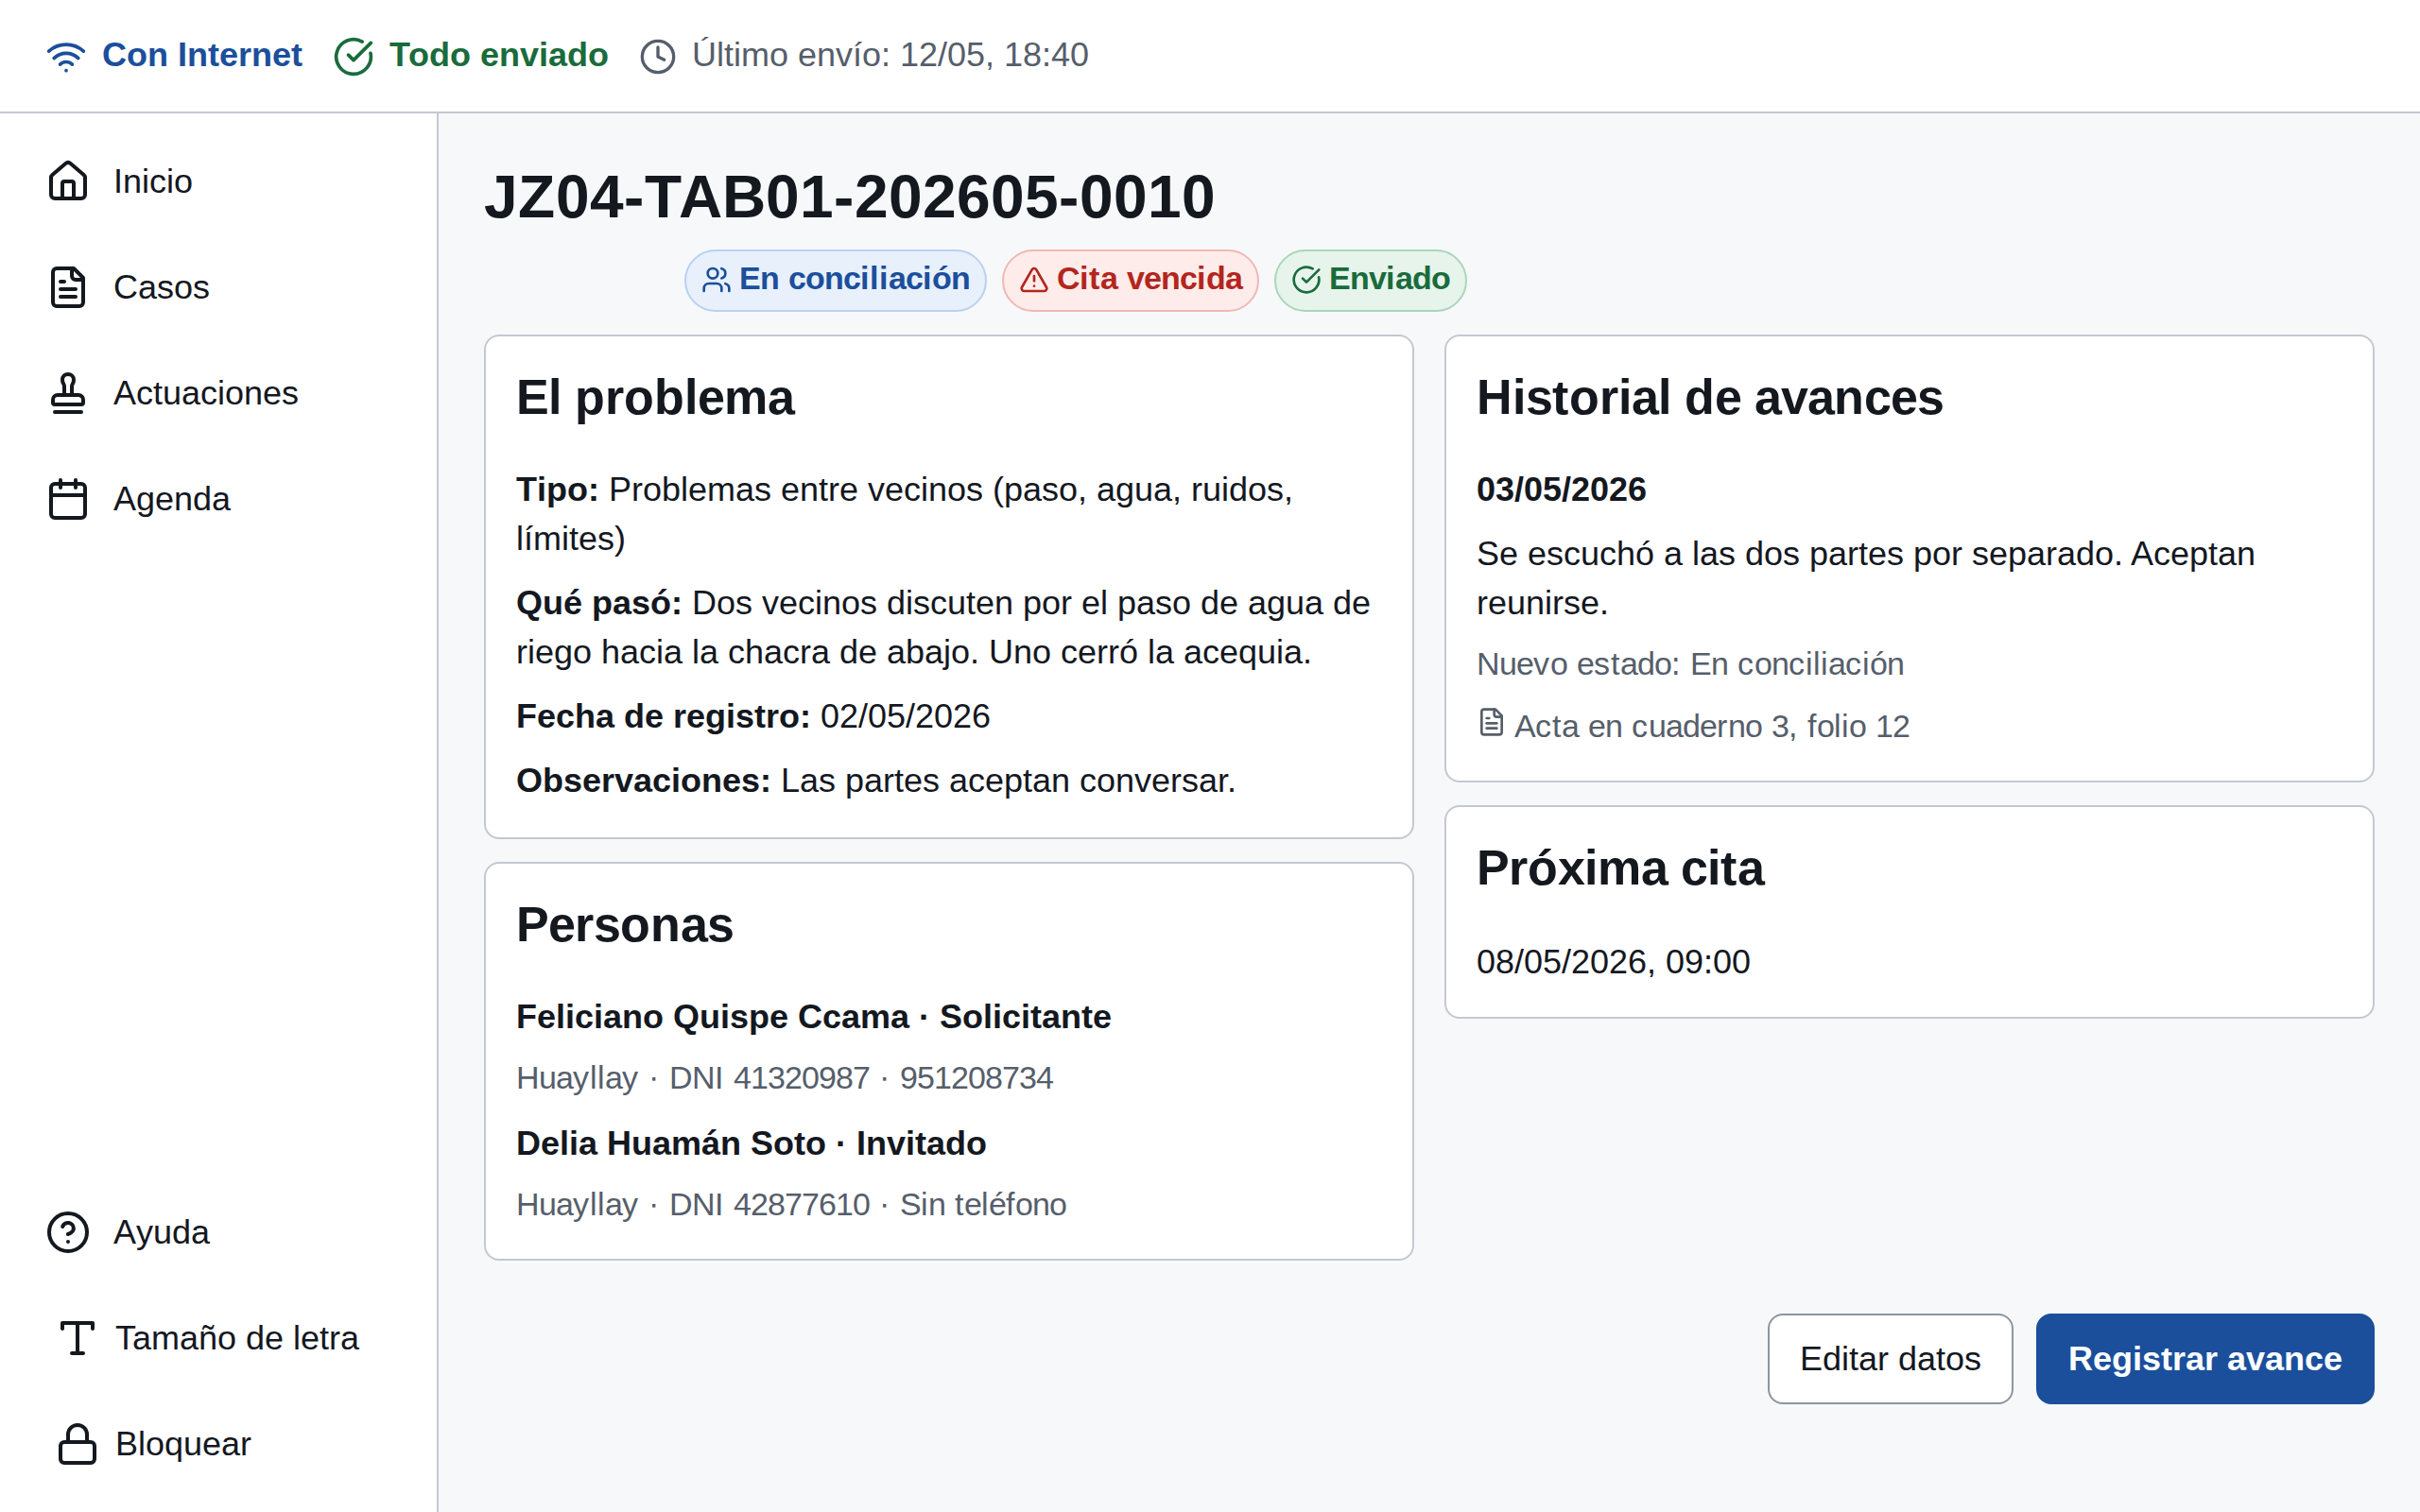
\includegraphics[width=0.86\linewidth]{capturas/P-04_caso-detalle.png}
\caption{P-04 · Estado normal. Detalle del caso con historial de avances y acciones}
\end{figure}


\section{Módulo 2 · Actuaciones}

\subsection{Dos dimensiones separadas}

El estado de atención (\textbf{Pendiente}, \textbf{Atendida}, \textbf{Concluida}) lo elige la jueza y responde a en qué punto va el trámite. El estado del registro (\textbf{Borrador} o \textbf{Completo}) es automático y responde a si faltan datos. Los dos se muestran juntos en el encabezado del formulario, cada uno con su rótulo.

En la pantalla, los tres estados de atención van explicados en una línea: Pendiente = la persona lo pidió, aún no se atiende; Atendida = ya se atendió, falta entregar; Concluida = ya se entregó.

\subsection{Campos del trámite}

\begin{center}
\small
\begin{tabular}{@{}p{3.0cm}p{2.4cm}p{8.8cm}@{}}
\toprule
\textbf{Campo} & \textbf{Obligatoriedad} & \textbf{Validación y mensaje} \\
\midrule
Código & Automático & \texttt{NOT-TAB01-202605-0007}, generado en la tableta \\
Fecha de solicitud & Obligatorio & «La fecha de solicitud no puede ser posterior a hoy.» \\
Tipo de actuación & Obligatorio & «Elija qué trámite le piden.» \\
Descripción o asunto & Obligatorio & «Cuente en pocas palabras qué necesita la persona.» \\
Estado de atención & Obligatorio & Prellenado en Pendiente \\
Fecha de atención & Condicional & Desde Atendida. «La atención no puede ser antes de la solicitud.» \\
Resultado & Condicional & Para Concluida. «Para concluir, escriba qué se entregó o qué constancia se emitió.» \\
Fecha de entrega & Condicional & Para Concluida. «La entrega no puede ser antes de la atención.» \\
Observaciones & Opcional & --- \\
Documentos & Opcional & Foto o referencia al documento físico \\
\bottomrule
\end{tabular}
\end{center}

Los participantes usan los mismos campos que las partes del caso, con la participación: Solicitante, Declarante o Testigo.

\subsection{Catálogo de trámites}

Se toma de las competencias notariales del juez de paz en la Ley 29824. Cada tarjeta muestra la etiqueta cotidiana como título y el término legal en gris debajo.

\begin{center}
\small
\begin{tabular}{@{}p{7.6cm}p{7.2cm}@{}}
\toprule
\textbf{Etiqueta cotidiana} & \textbf{Término legal} \\
\midrule
Certificar una firma & Legalización de firma \\
Certificar una copia de documento & Copia certificada \\
Constancia de que vive en un lugar & Constancia domiciliaria \\
Constancia de que una persona sigue con vida & Constancia de supervivencia \\
Constancia de que ocupa un terreno & Constancia de posesión \\
Constancia de que viven juntos & Constancia de convivencia \\
Documento de venta o traspaso de un bien & Transferencia de bienes, dentro de los montos que permite la ley \\
Otra (escribir cuál) & --- \\
\bottomrule
\end{tabular}
\end{center}

Se muestran los cuatro primeros y un botón \textbf{Ver más trámites}. El motivo no es solo reducir el número de opciones: con tarjetas descriptivas el problema real es la carga de lectura.

\subsection{Personas y trámites repetidos}

La aplicación compara por DNI si existe y, si no, por nombre parecido más la misma comunidad. Para trámites añade el mismo tipo y una fecha de solicitud dentro de siete días. Siempre \textbf{advierte sin bloquear}: muestra el registro parecido con sus datos y ofrece dos caminos. Sin Internet solo se detectan repetidos dentro de la tableta; los que existan en el Poder Judicial se revisan al enviar.

\begin{figure}[H]\centering
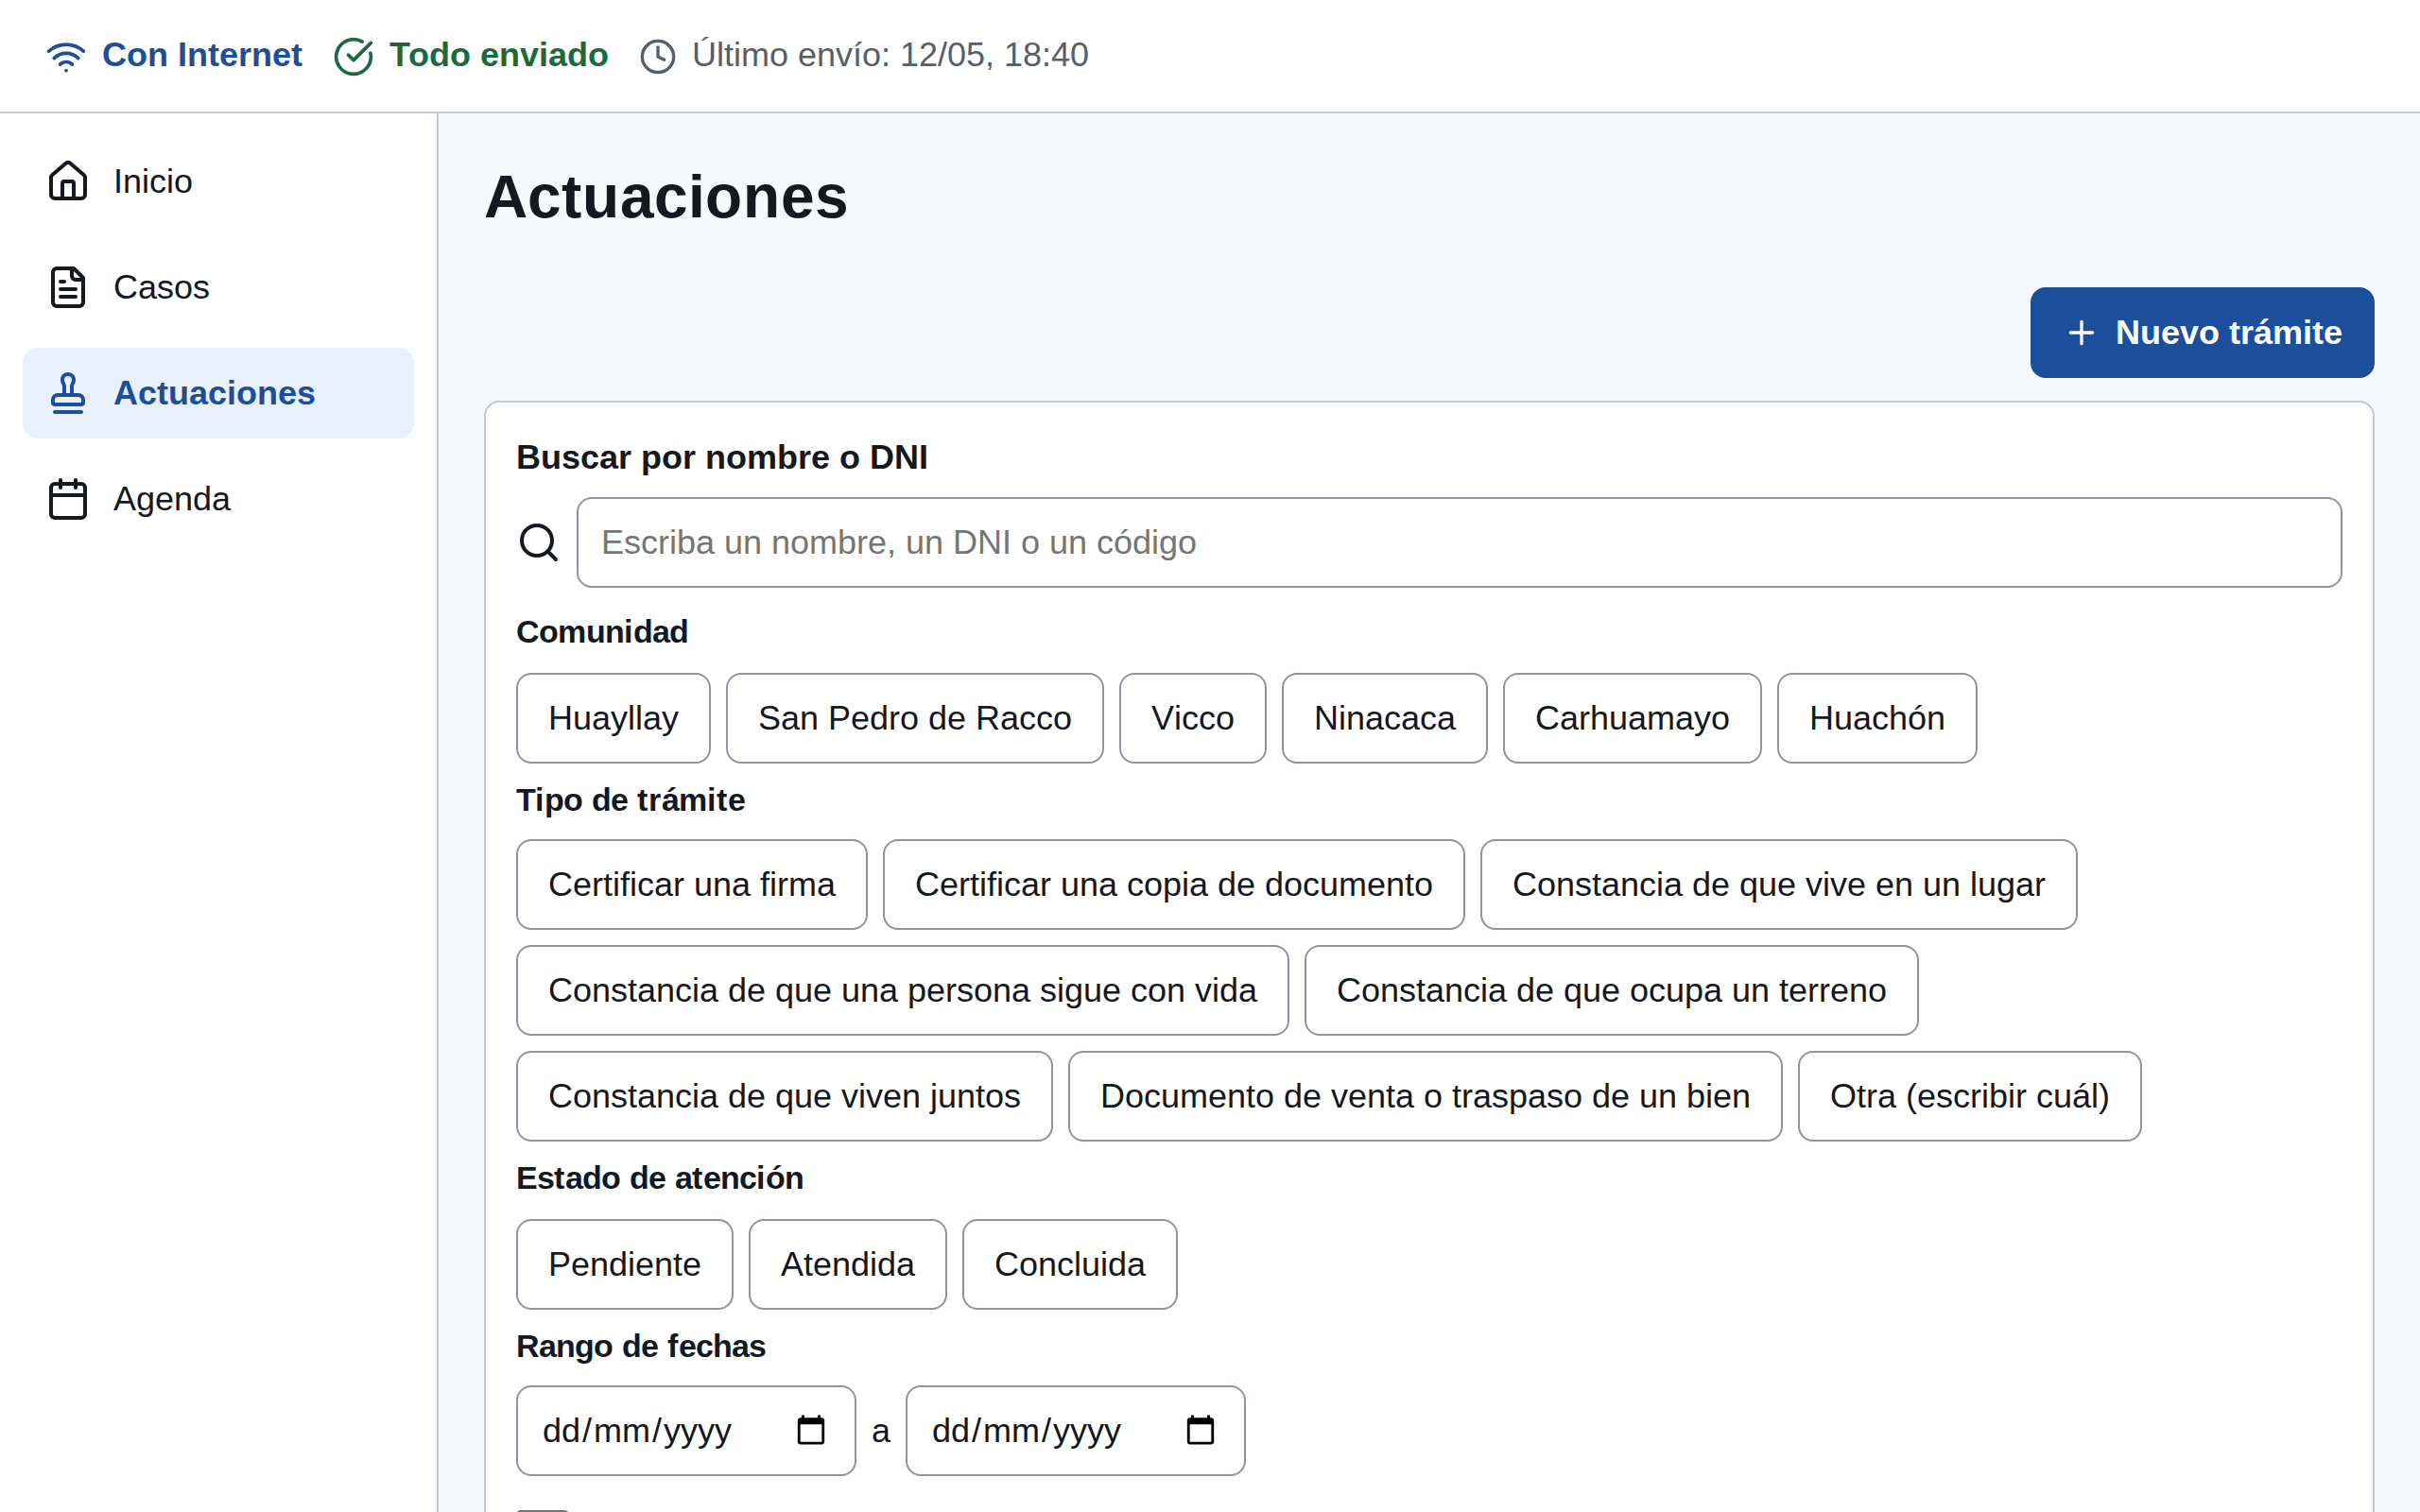
\includegraphics[width=0.86\linewidth]{capturas/P-05_actuaciones-lista.png}
\caption{P-05 · Estado normal. Lista de trámites con estados de atención y borradores}
\end{figure}
\begin{figure}[H]\centering
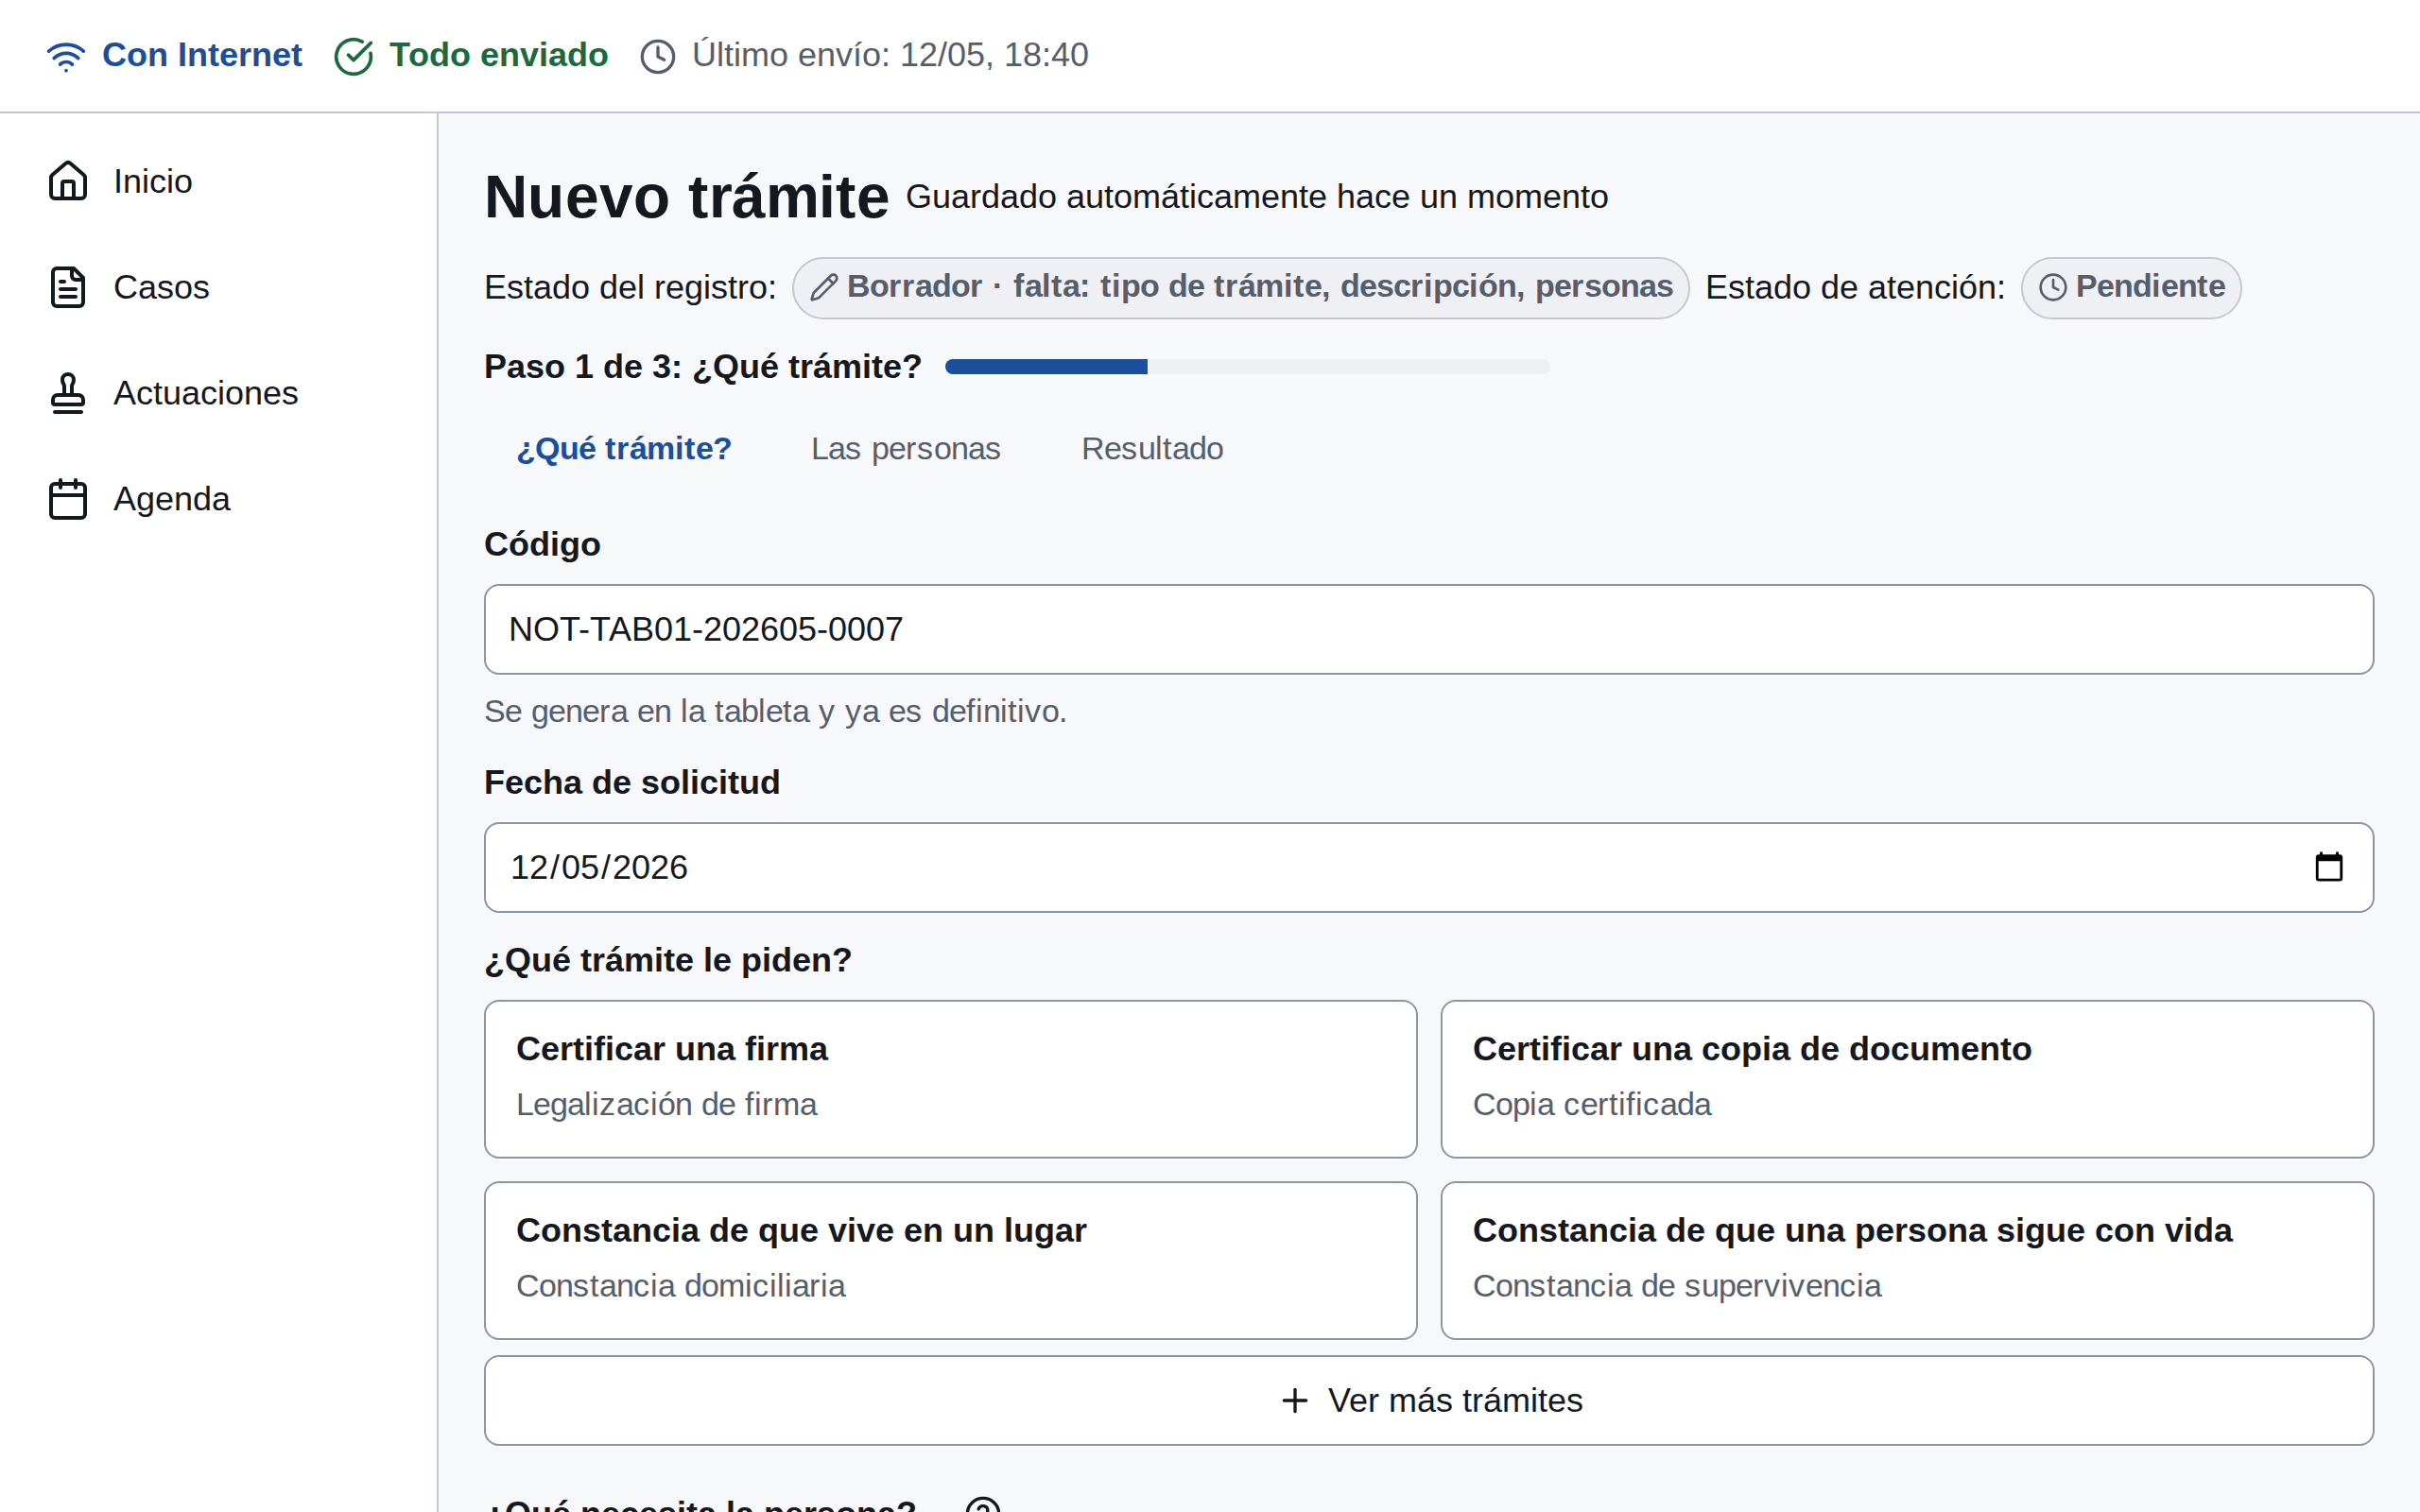
\includegraphics[width=0.86\linewidth]{capturas/P-06_actuacion-nueva.png}
\caption{P-06 · Estado normal. Catálogo de trámites en tarjetas, 4 primero y Ver más}
\end{figure}


\section{Módulo 3 · Agenda}

\subsection{Vistas y categorías}

Tres vistas con un selector grande: \textbf{Mes}, \textbf{Semana} y \textbf{Día}, más un botón \textbf{Hoy}. Las cuatro categorías llevan color, ícono y texto: Audiencia, Reunión, Visita a comunidad y Otra. Los tres estados también: Programada, Realizada y Cancelada, esta última con el texto tachado en gris.

En la vista mes cada día muestra hasta tres actividades y cuenta el resto con «+2 más»; tocar el día abre la vista día.

\subsection{Campos de la actividad}

\begin{center}
\small
\begin{tabular}{@{}p{3.0cm}p{2.4cm}p{8.8cm}@{}}
\toprule
\textbf{Campo} & \textbf{Obligatoriedad} & \textbf{Validación y mensaje} \\
\midrule
Título & Obligatorio & Con sugerencias. «Escriba un nombre para la actividad.» \\
Categoría & Obligatorio & «Elija el tipo de actividad.» \\
Fecha & Obligatorio & Si es pasada, aviso que no bloquea \\
Hora de inicio & Opcional & Casilla «Sin hora fija» \\
Hora de término & Condicional & «La hora de término debe ser después de la de inicio.» \\
Lugar o comunidad & Obligatorio & «Indique dónde será.» \\
Descripción o motivo & Opcional & --- \\
Estado & Obligatorio & Prellenado en Programada \\
Vínculo & Opcional & Buscar un caso o un trámite \\
Recordatorio & Opcional & Prellenado en «1 día antes» \\
\bottomrule
\end{tabular}
\end{center}

\subsection{Avisos y vínculo con los casos}

Si la hora nueva choca con otra actividad, la aplicación lo dice mostrando cuál: «A esa hora ya tiene: Visita a Huayllay», y deja agendar igual. Los recordatorios se muestran dentro de la aplicación, no con las notificaciones del navegador. Cuando un caso recibe una próxima fecha de atención, la actividad se crea sola y queda vinculada; desde la actividad se vuelve al caso con un toque.

\begin{figure}[H]\centering
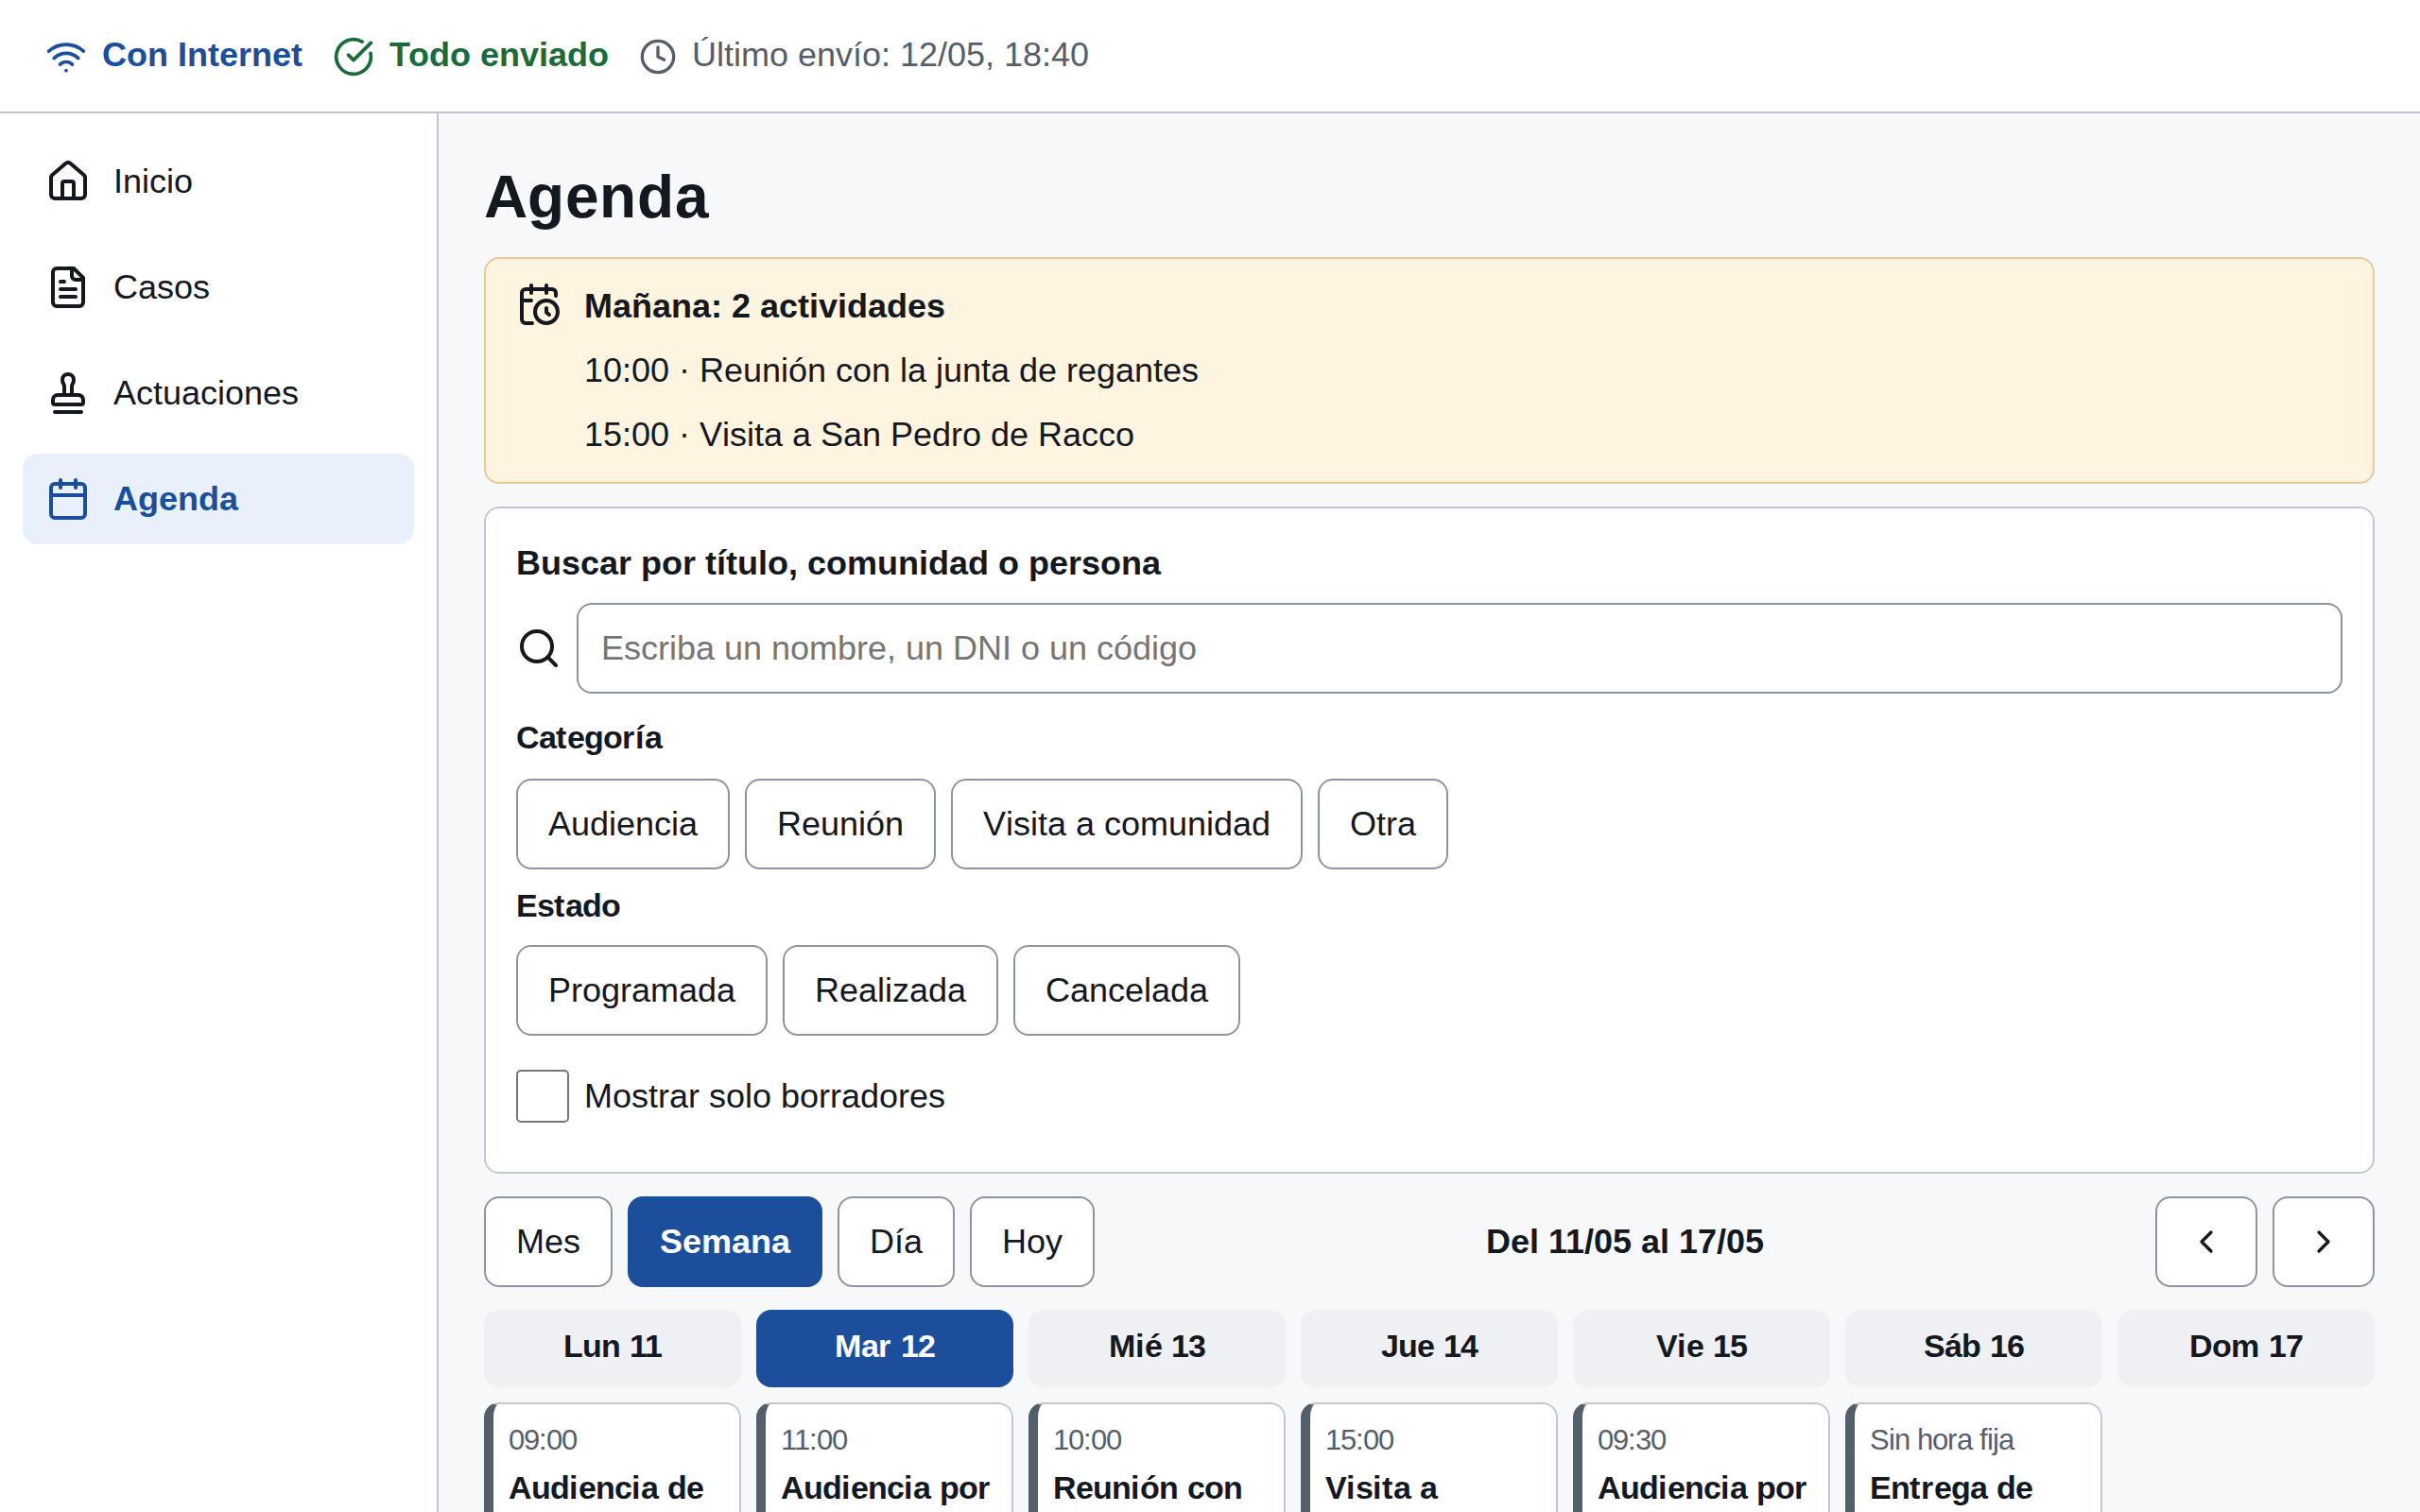
\includegraphics[width=0.86\linewidth]{capturas/P-07_agenda-semana.png}
\caption{P-07 · Estado normal. Agenda en vista semana con categorías y estados}
\end{figure}
\begin{figure}[H]\centering
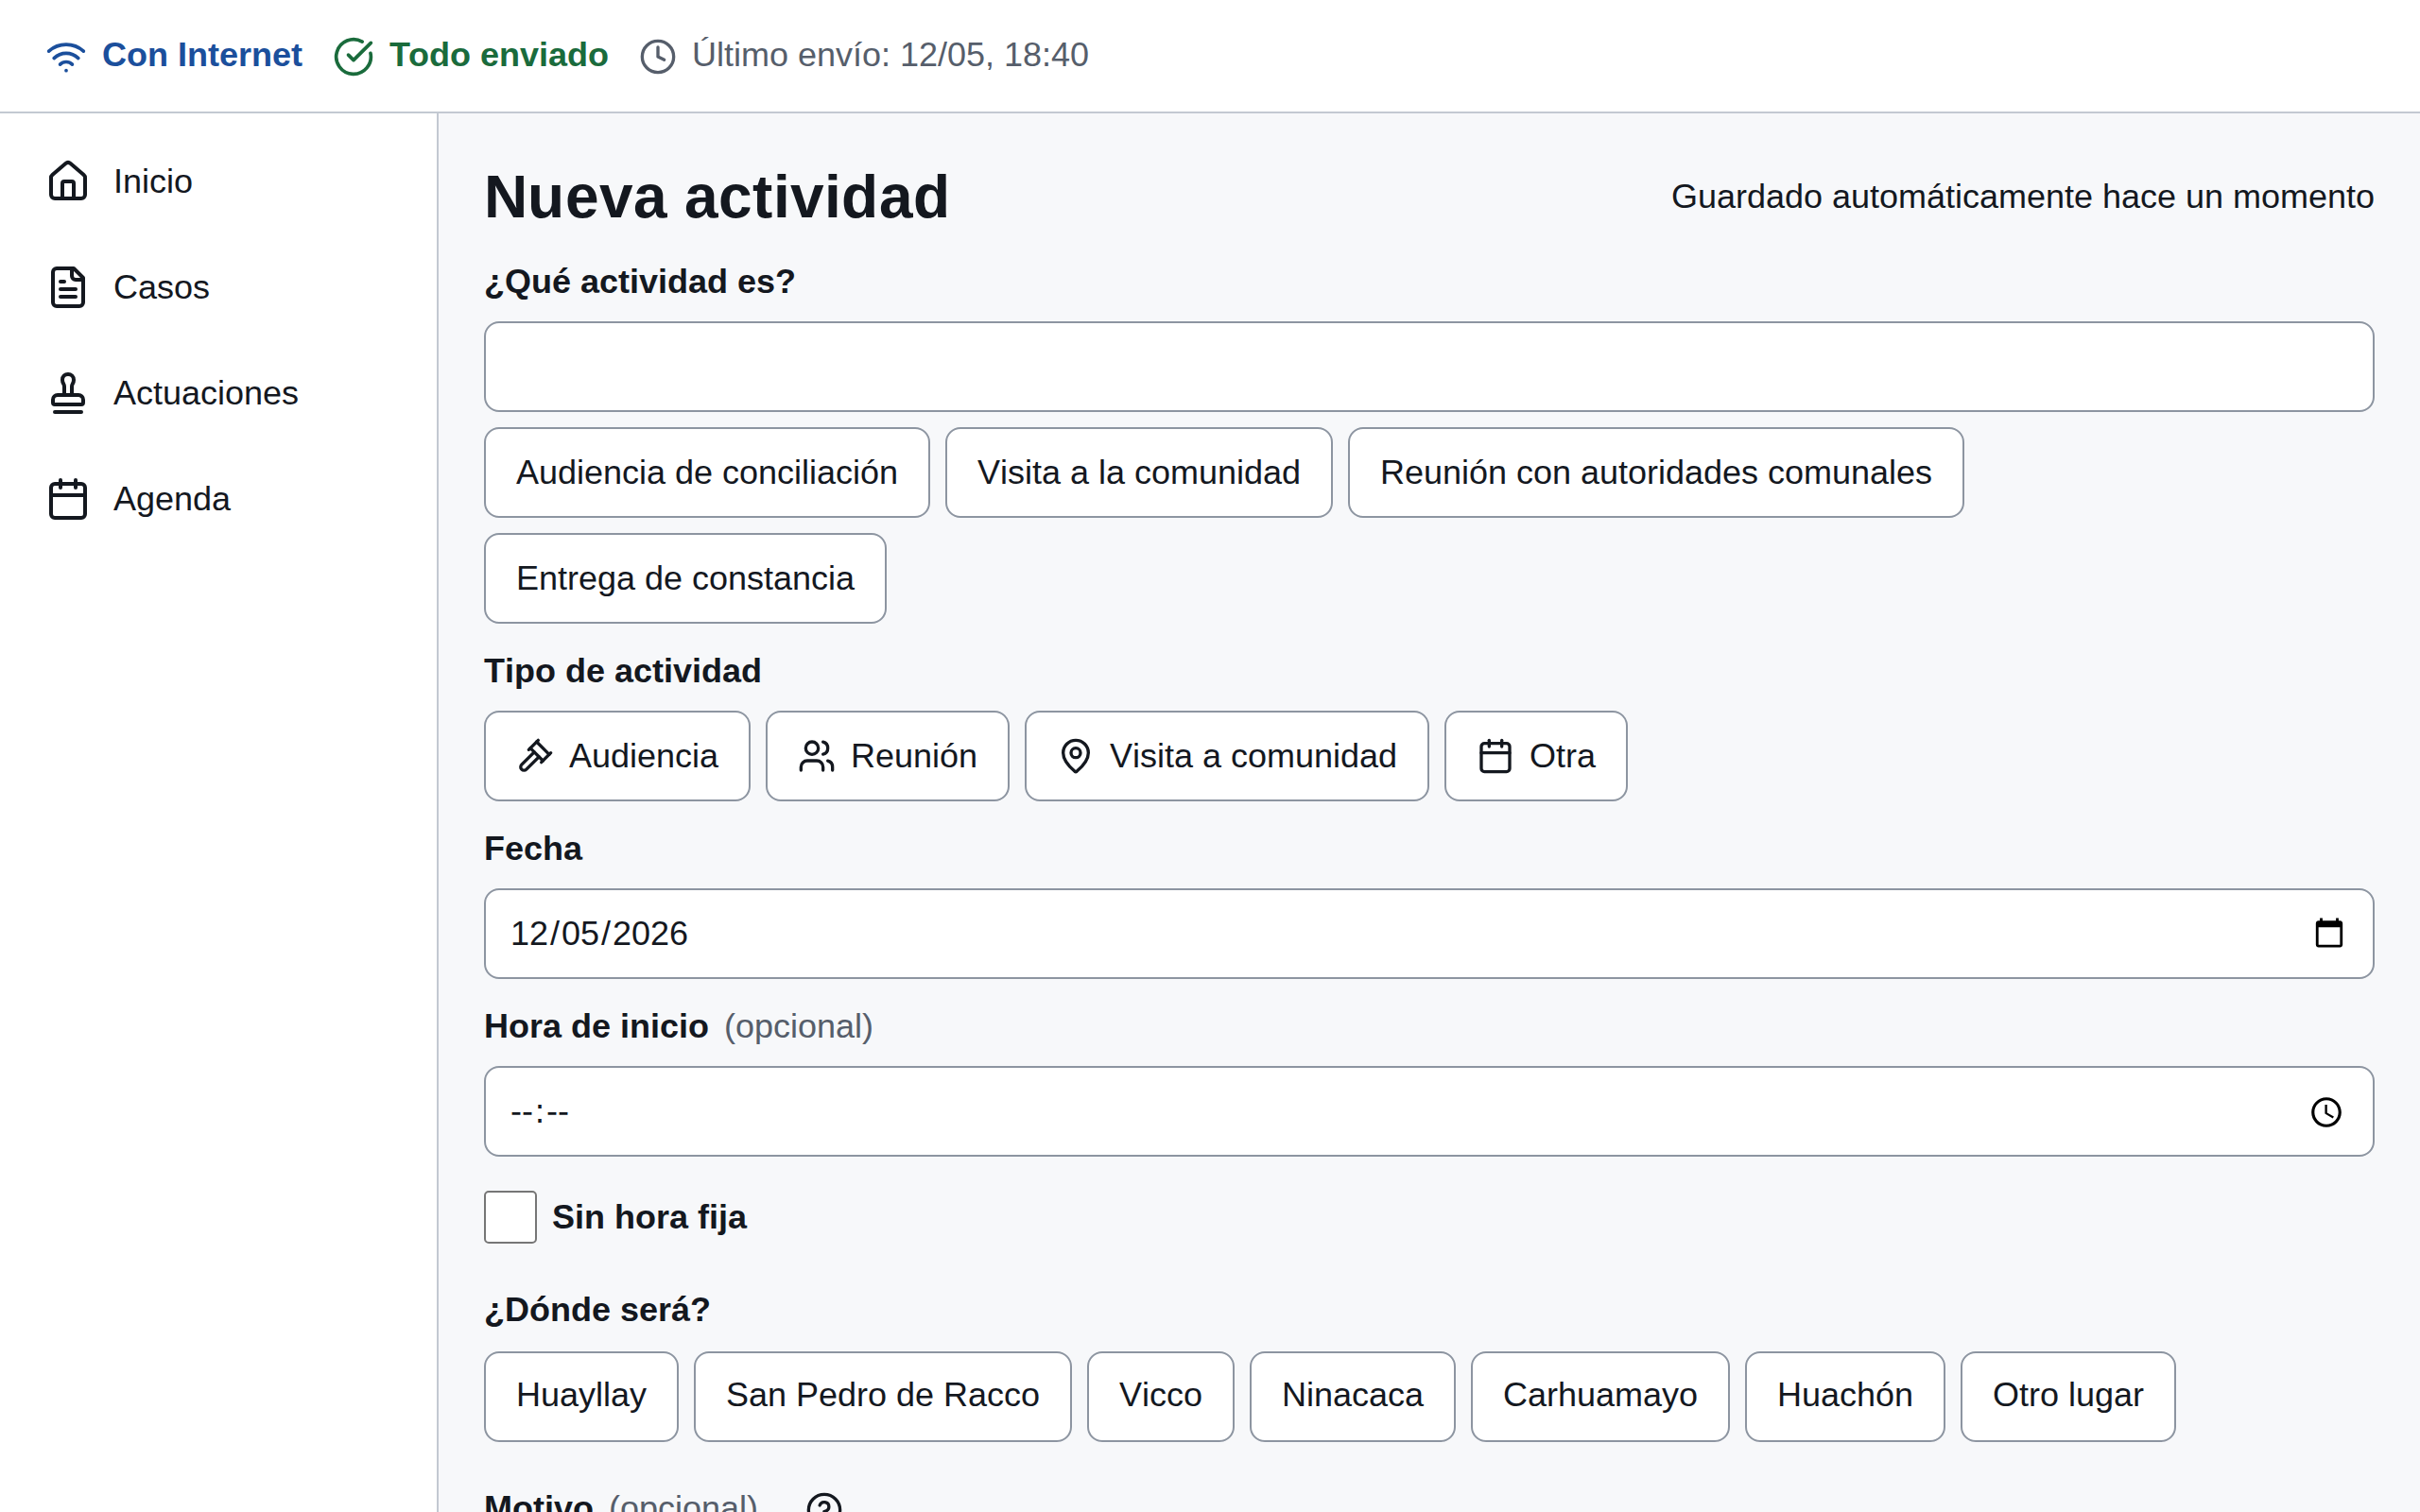
\includegraphics[width=0.86\linewidth]{capturas/P-08_actividad-nueva.png}
\caption{P-08 · Estado normal. Formulario de actividad con todos sus campos}
\end{figure}


\section{Envío al Poder Judicial y vista en computadora}

\subsection{Cómo se envía}

Al detectar Internet la aplicación \textbf{envía sola} y muestra el progreso; también existe el botón \textbf{Enviar ahora}. El envío automático se eligió porque a una usuaria con poca experiencia se le puede olvidar hacerlo a mano, y el resultado siempre se confirma. La tableta puede enviar desde cualquier lugar con Internet, no solo desde la sede.

\subsection{Los cuatro resultados posibles}

\begin{center}
\small
\begin{tabular}{@{}p{3.0cm}p{11.8cm}@{}}
\toprule
\textbf{Resultado} & \textbf{Qué dice la aplicación} \\
\midrule
Éxito total & «Se enviaron los 4 registros. Todo está guardado en el Poder Judicial.» \\
Corte a mitad & «Se enviaron 2 de 4. Se cortó el Internet. Los otros 2 siguen seguros en la tableta.» Con Reintentar \\
Error del servidor & «El Poder Judicial no respondió. Sus 4 registros siguen seguros en la tableta.» Con Reintentar \\
Conflicto & Se aplica solo el cambio más reciente en cada campo y se informa cuál se usó. Con Ver y cambiar \\
\bottomrule
\end{tabular}
\end{center}

Los cuatro mensajes dicen siempre dónde quedaron los registros. El conflicto se resuelve solo para no exigir una comparación campo por campo a una usuaria con poca experiencia digital; la versión descartada queda en el historial y se puede recuperar desde \textbf{Ver y cambiar}.

Esta regla choca con la fecha editable del módulo 1: si el reloj de la tableta está desfasado, «el más reciente» puede elegir mal. Por eso la resolución automática nunca es silenciosa: siempre dice qué campo se tomó y de qué versión, la versión descartada queda en el historial y \textbf{Ver y cambiar} permite volver atrás. Un reloj desfasado puede hacer que la primera elección sea la equivocada, pero no puede hacer que se pierda nada.

\subsection{La vista en computadora}

Es la misma aplicación adaptada a una pantalla de 1440 por 900, con tablas de más columnas y el verbo «Haz clic» en lugar de «Toca». Muestra únicamente lo que ya llegó al Poder Judicial y lo declara: «La tableta envió datos por última vez el 12/05, 18:40. Lo que registró después aún no aparece aquí.» Nunca afirma cuántos registros tiene pendientes la tableta, porque desde ahí eso no se puede saber. Desde la computadora también se consulta, crea y edita, y de ahí nacen los conflictos.

\begin{figure}[H]\centering
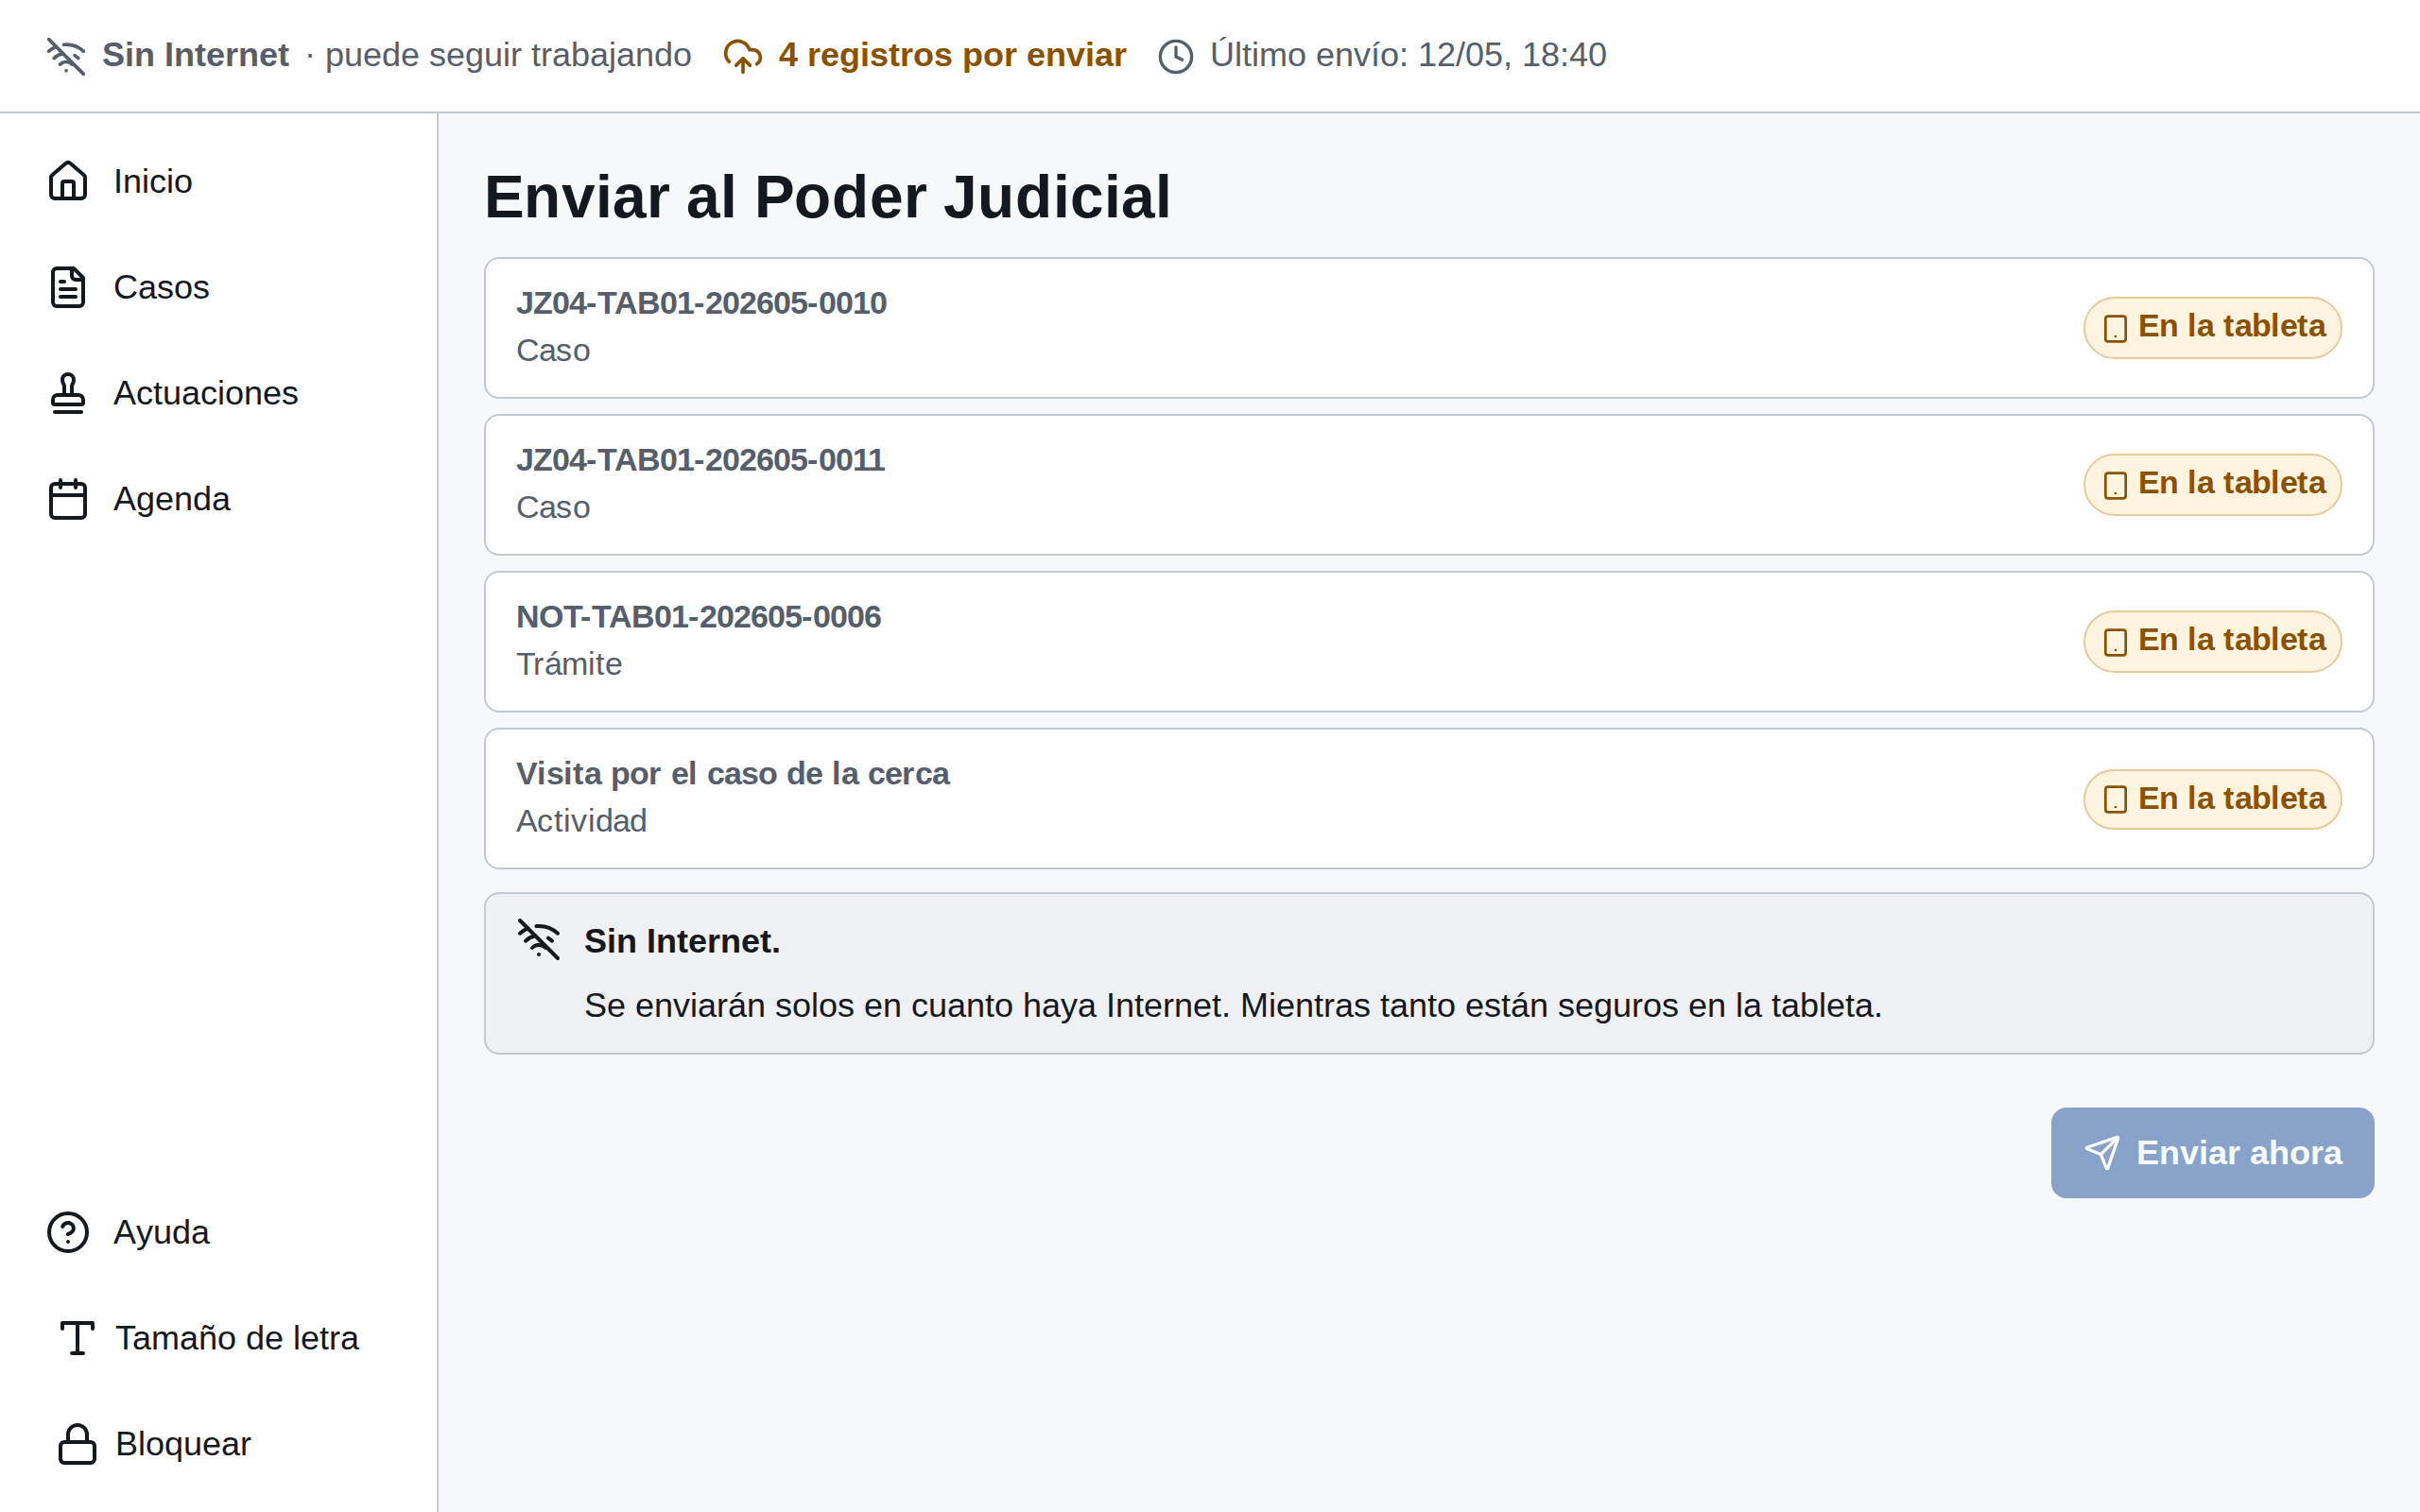
\includegraphics[width=0.86\linewidth]{capturas/P-09_envio-pendientes.png}
\caption{P-09 · Antes de enviar. Lista de registros por enviar y botón Enviar ahora}
\end{figure}
\begin{figure}[H]\centering
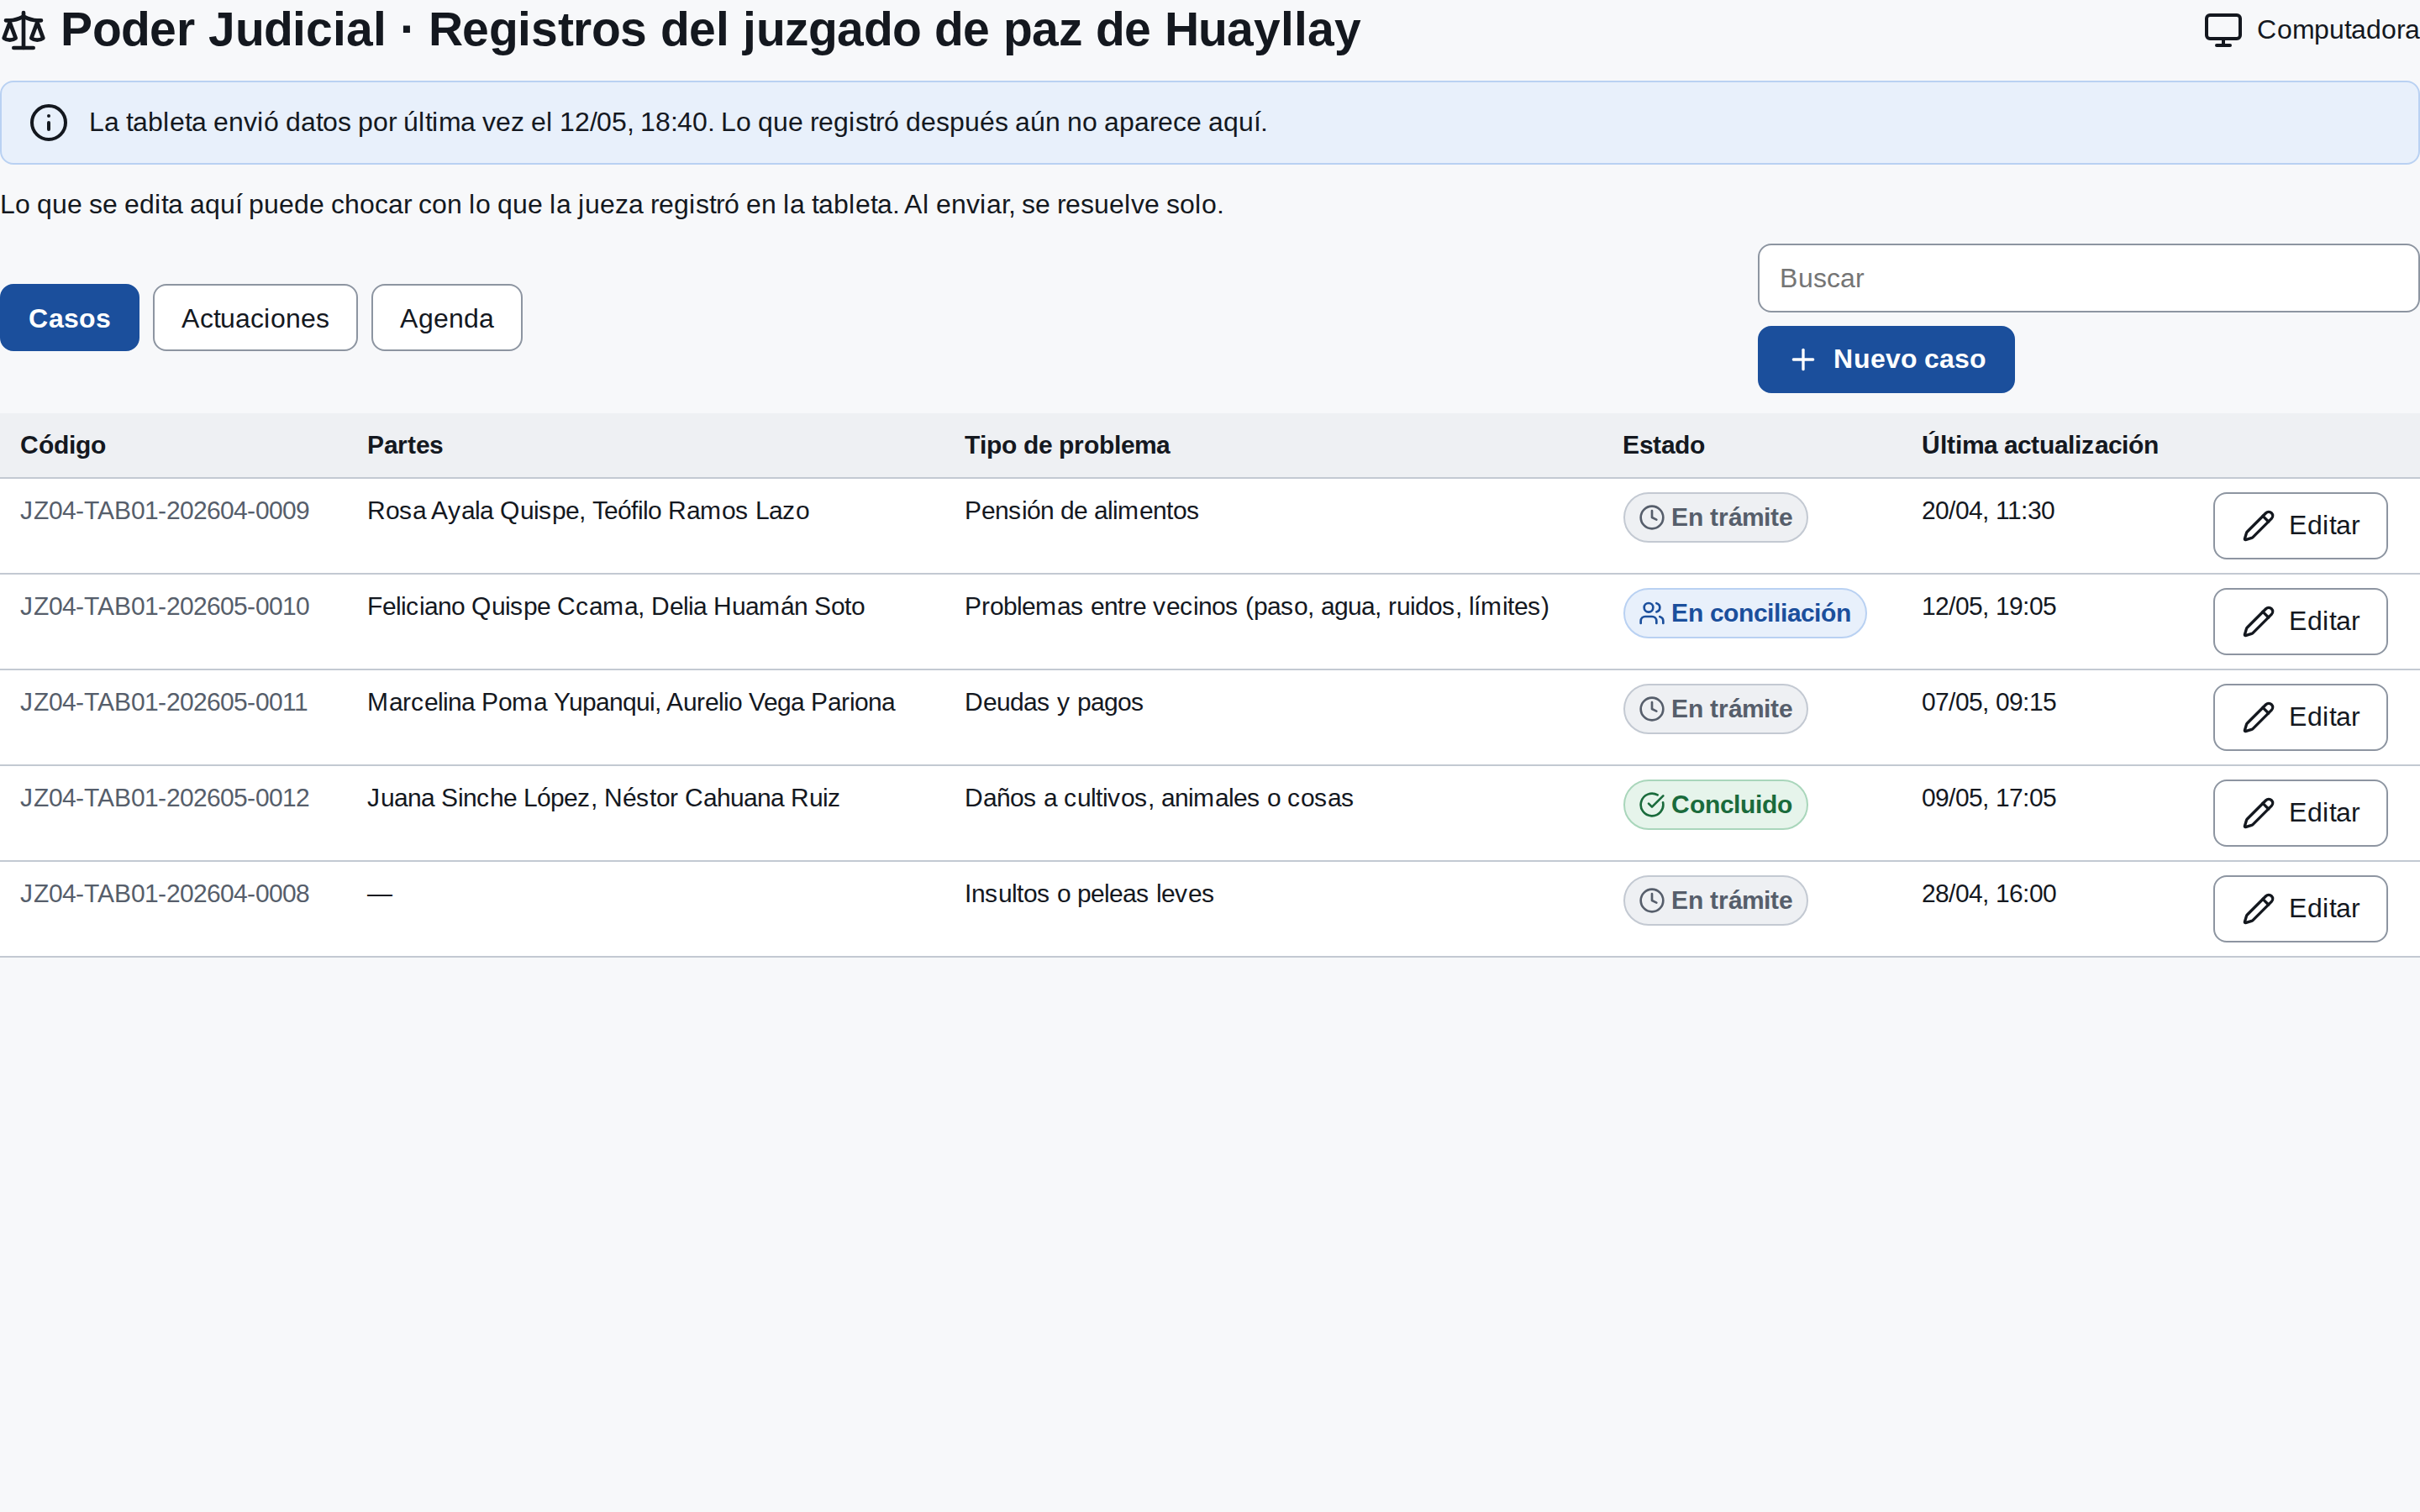
\includegraphics[width=0.86\linewidth]{capturas/P-10_computadora.png}
\caption{P-10 · Vista en computadora. Misma aplicación en 1440x900 con tablas y aviso del último envío de la tableta}
\end{figure}


\subsection{Las cuatro variantes del envío}

\begin{figure}[H]\centering
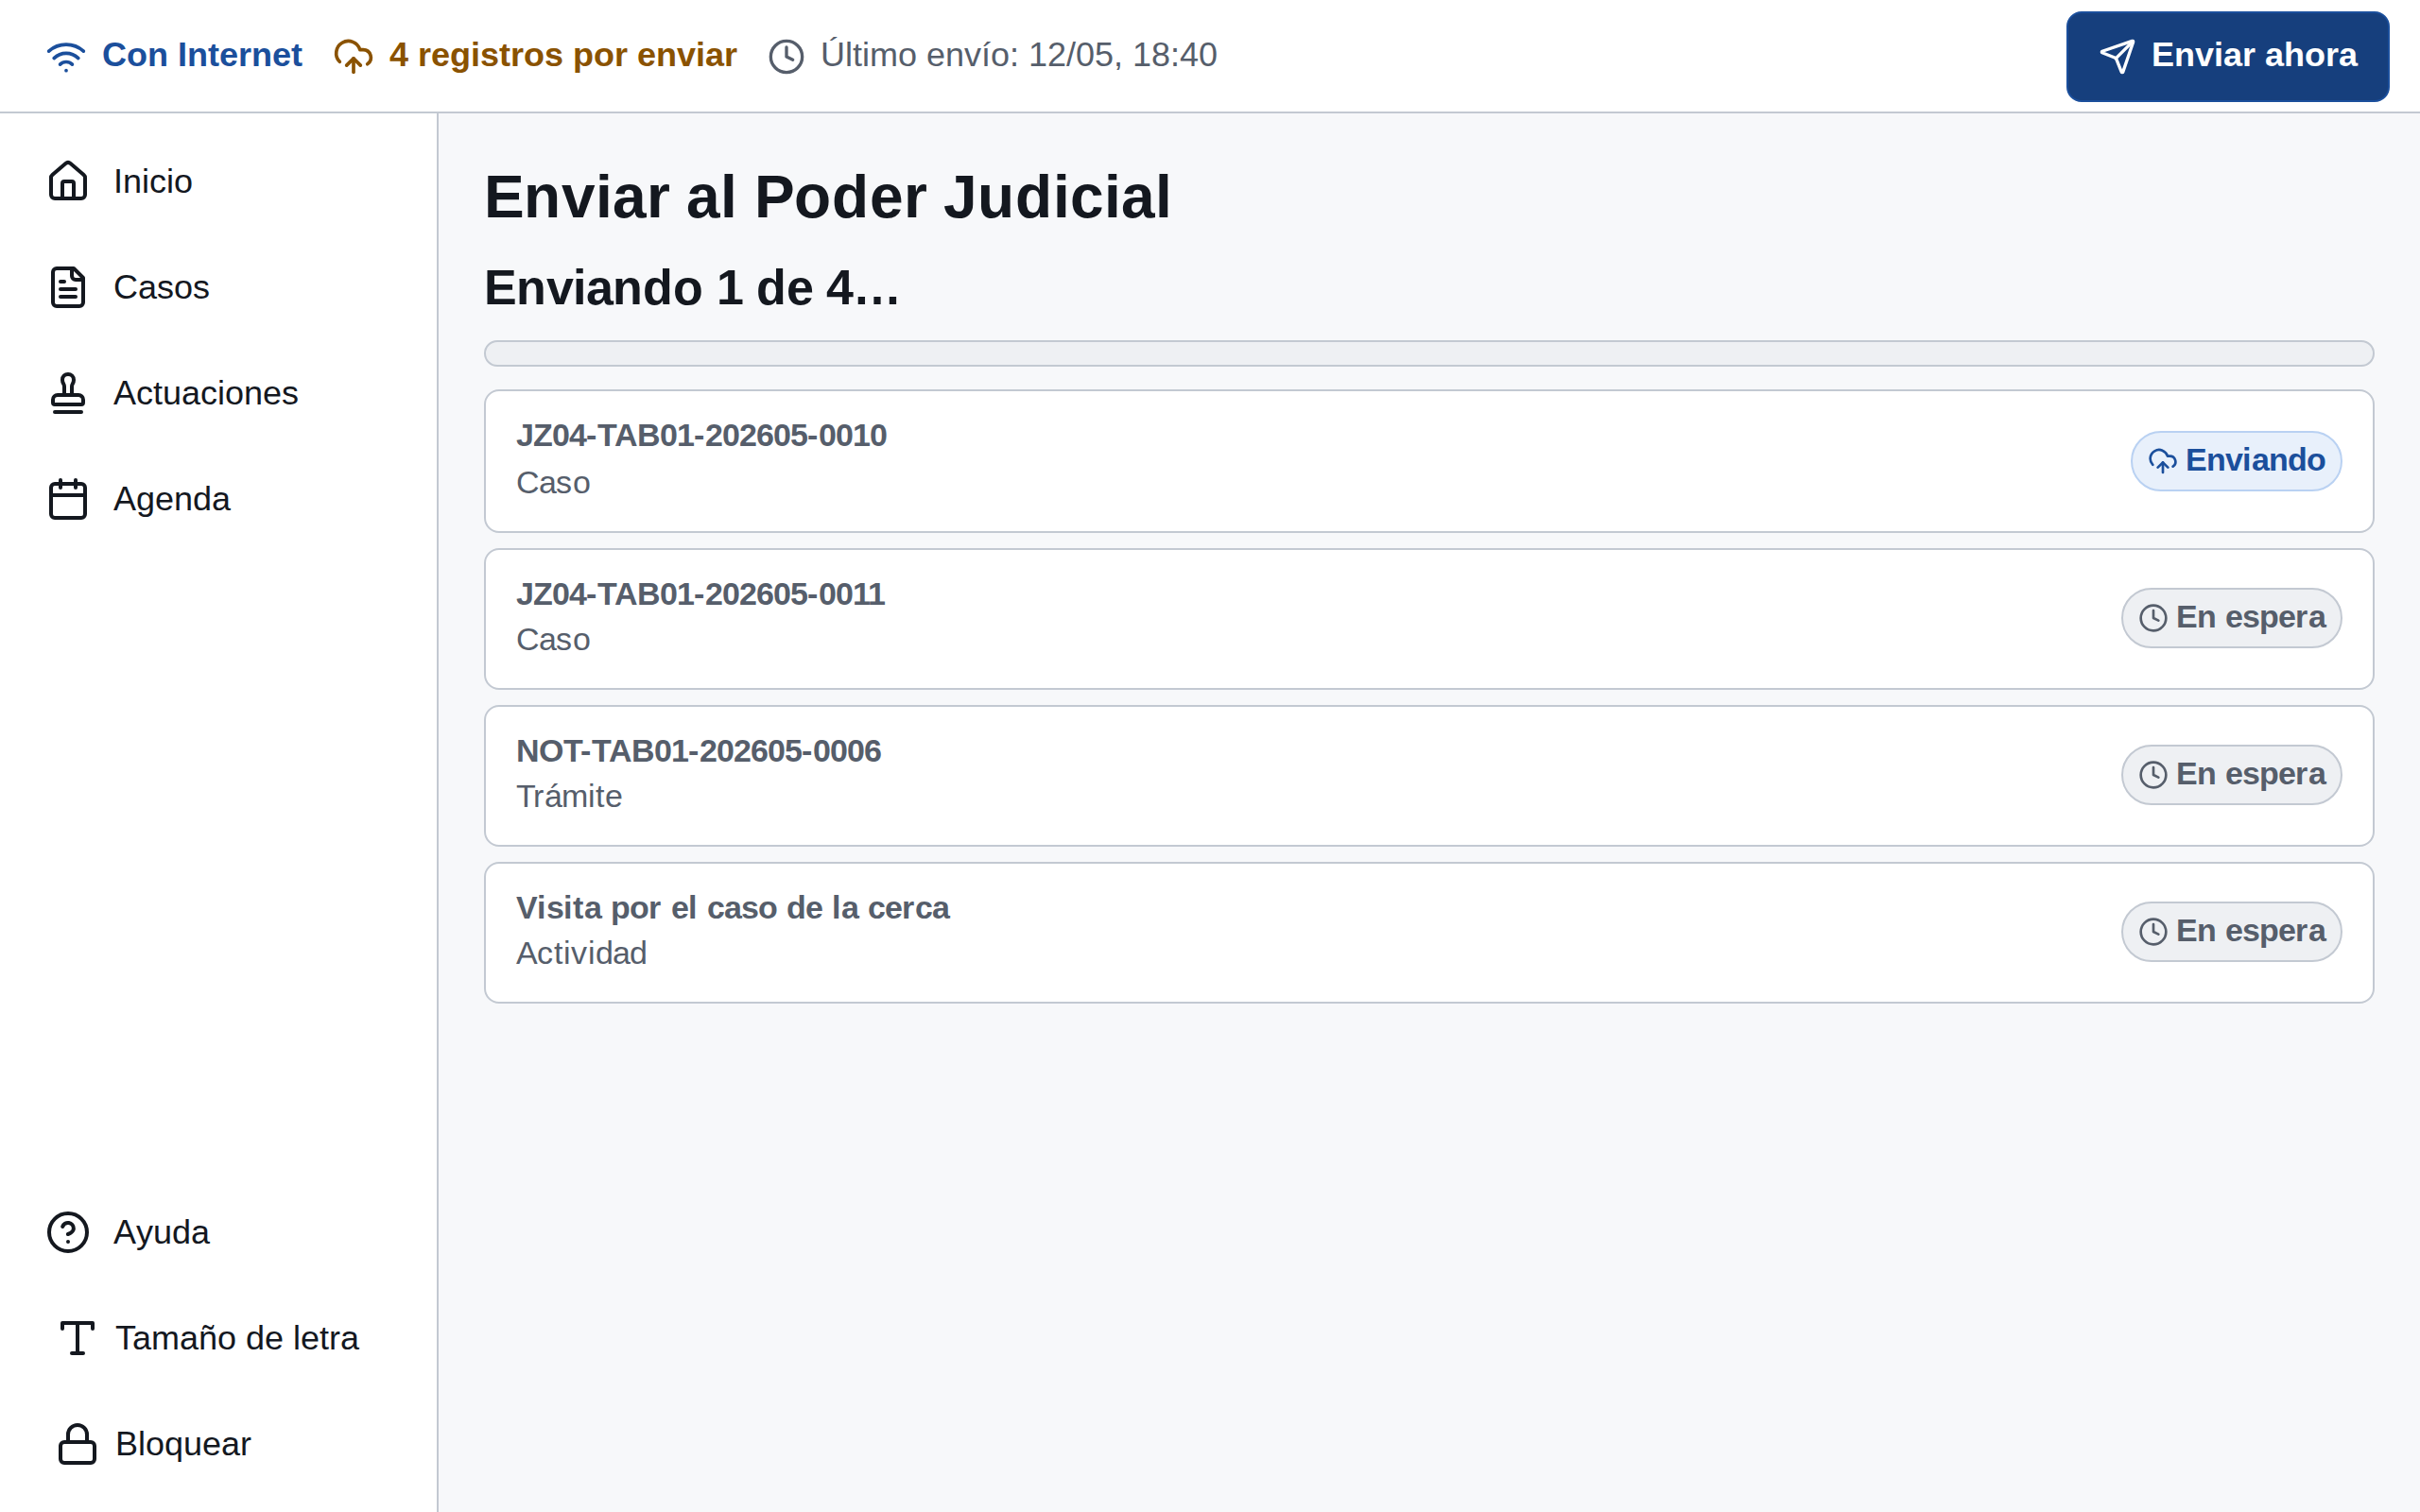
\includegraphics[width=0.82\linewidth]{capturas/P-09a_progreso.png}
\caption{P-09 · Progreso. Progreso con el número de registros y el estado de cada uno}
\end{figure}
\begin{figure}[H]\centering
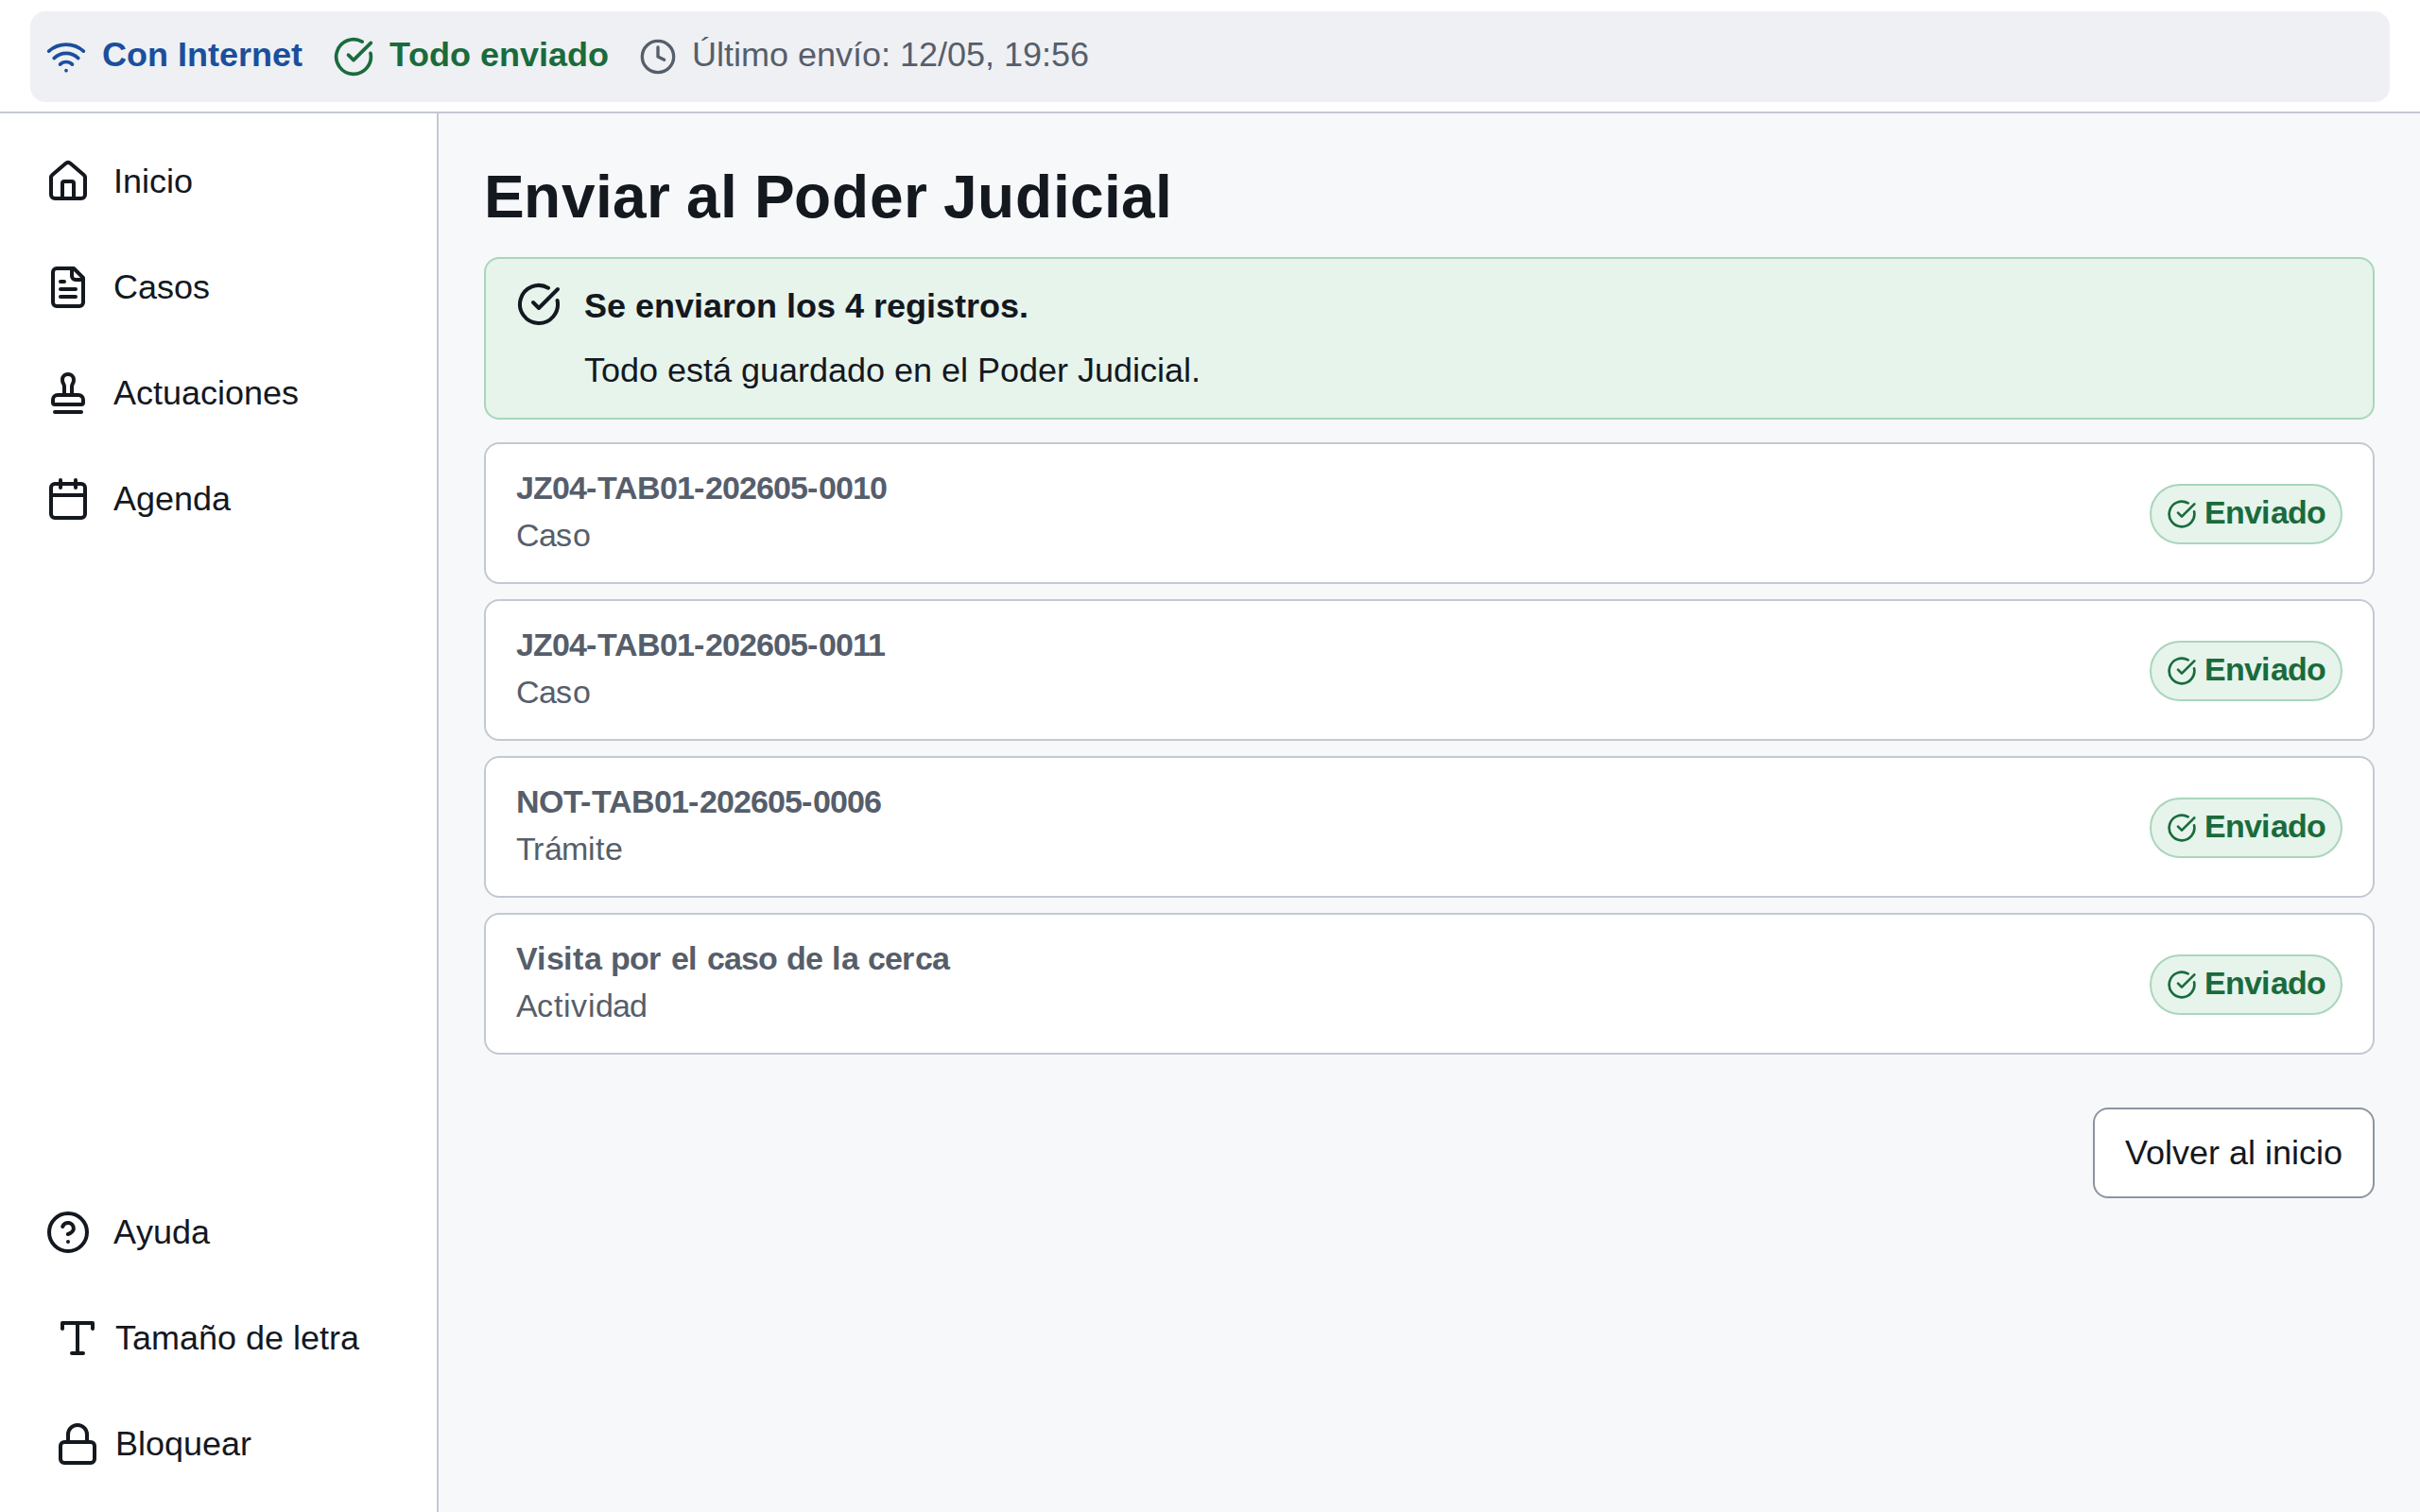
\includegraphics[width=0.82\linewidth]{capturas/P-09b_exito.png}
\caption{P-09 · sync-ok. Se enviaron los 4 registros y la barra pasa a Todo enviado}
\end{figure}
\begin{figure}[H]\centering
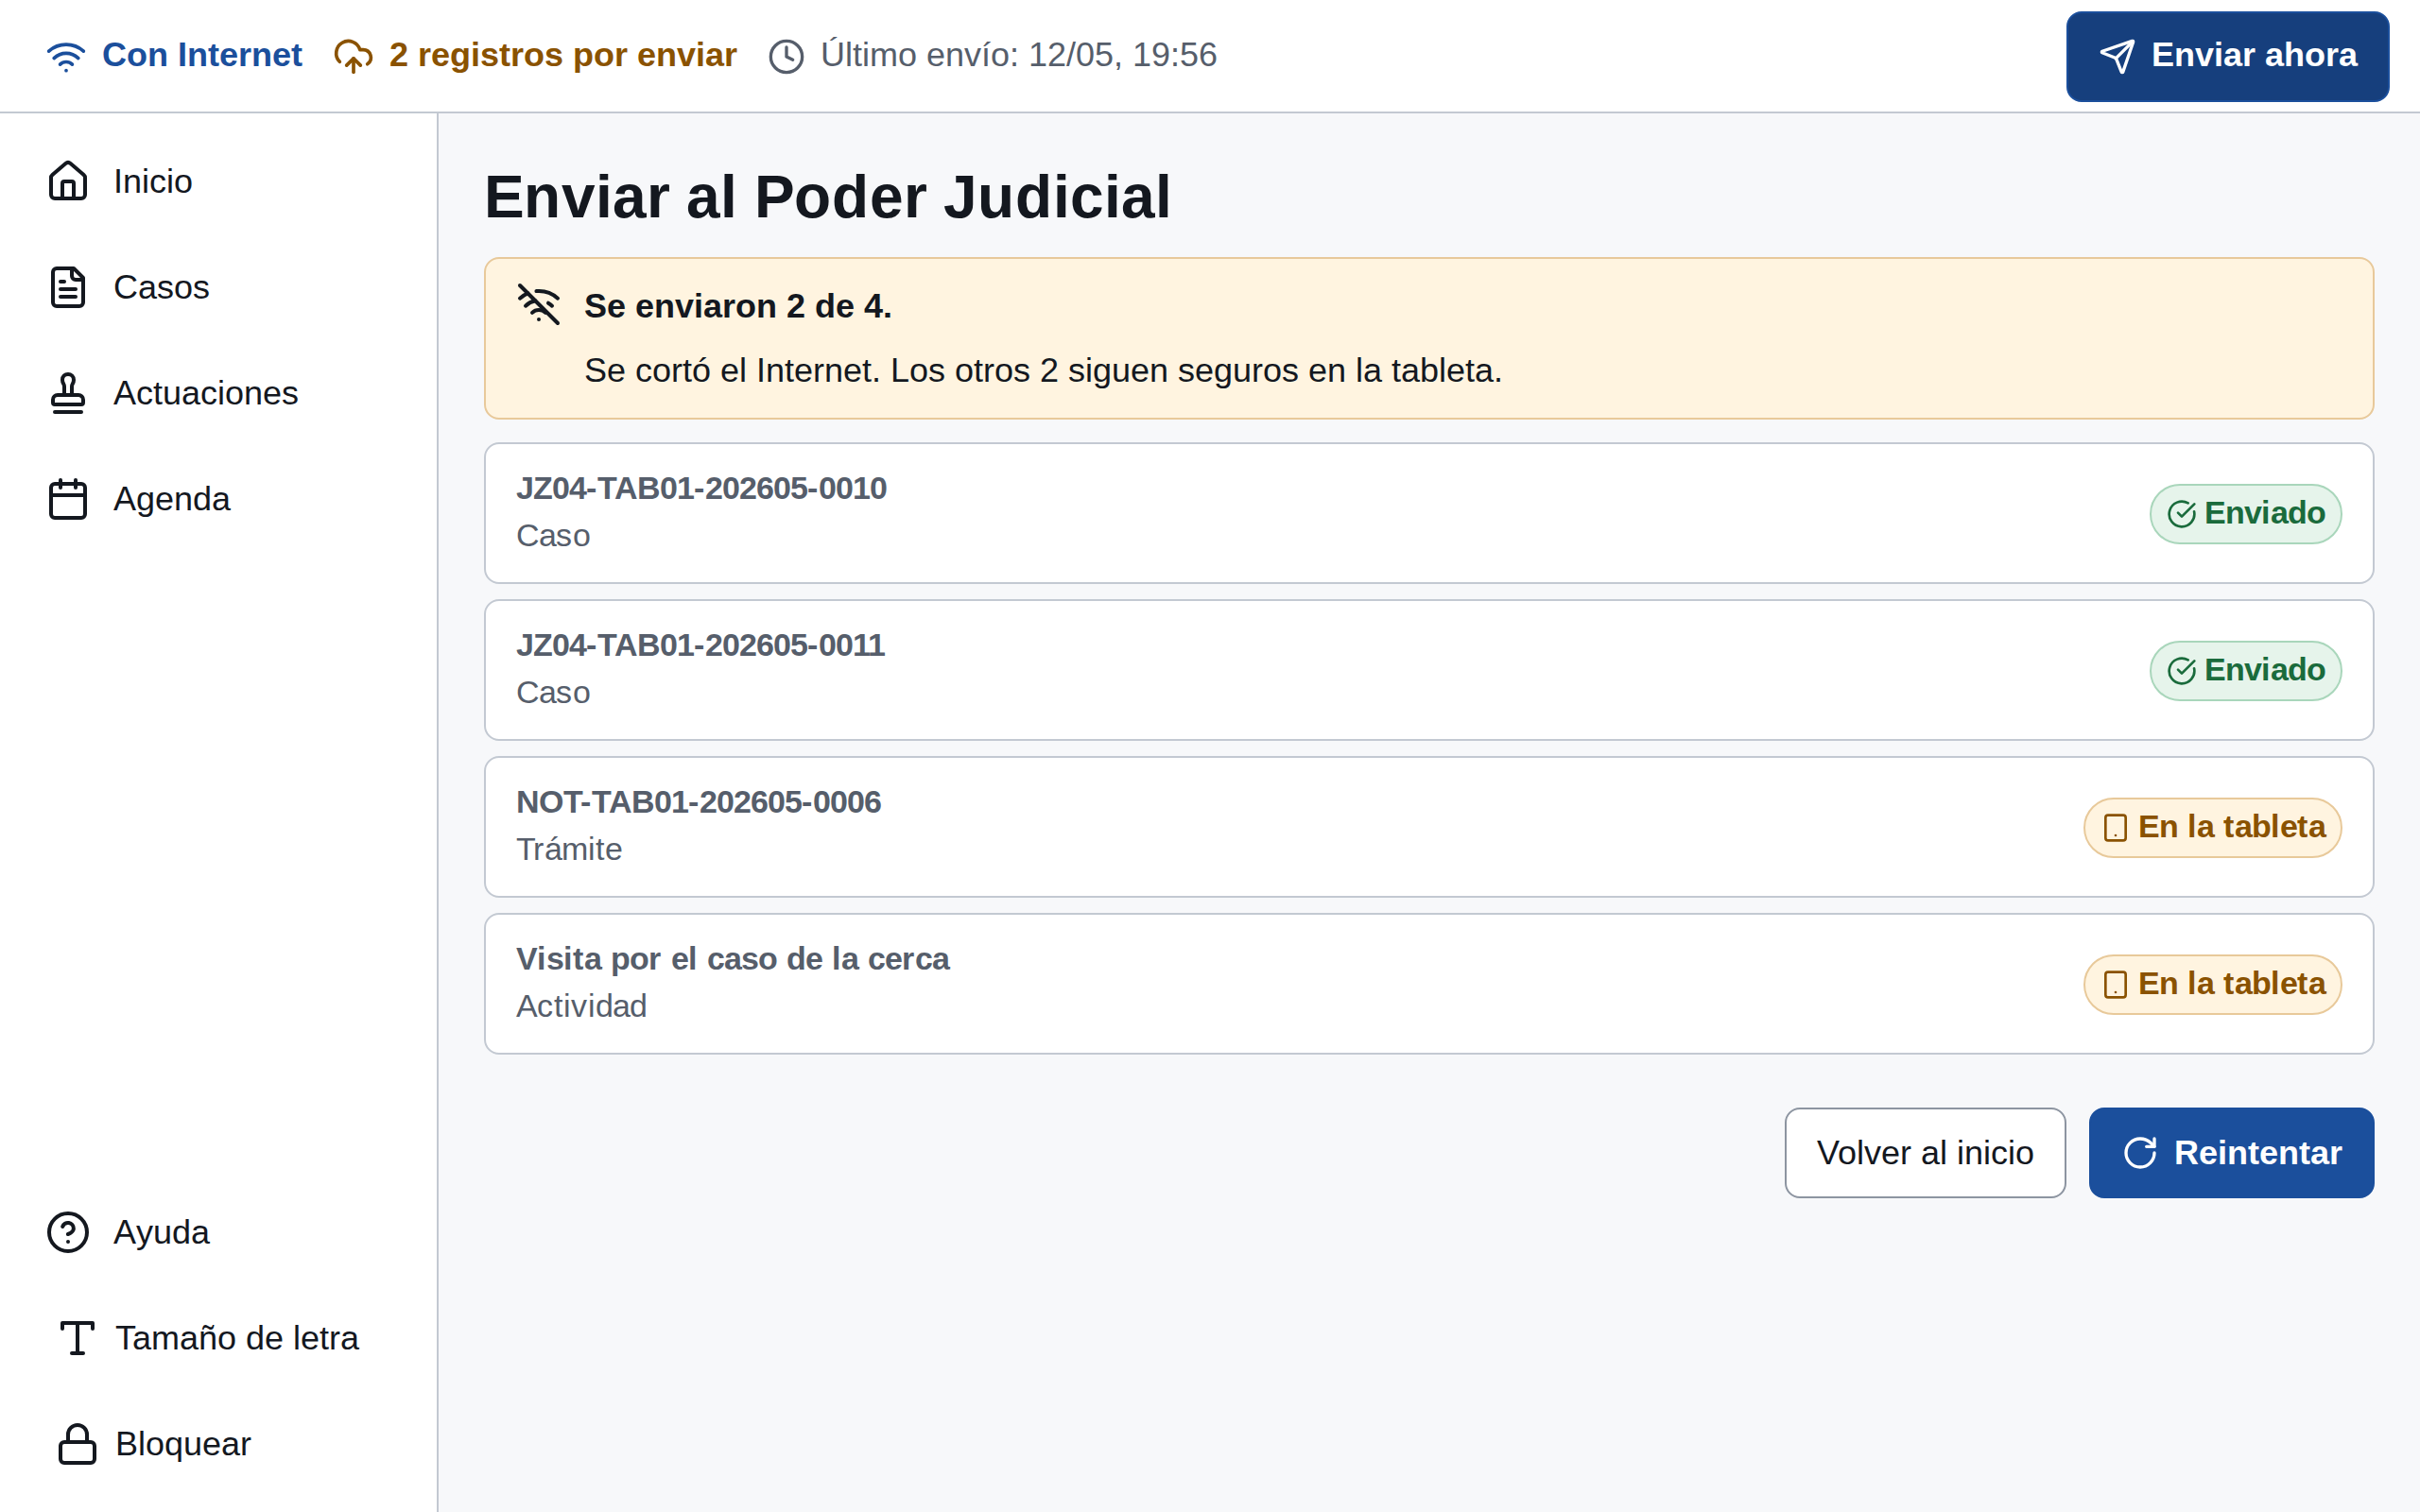
\includegraphics[width=0.82\linewidth]{capturas/P-09c_fallo-parcial.png}
\caption{P-09 · sync-partial. Se cortó el Internet a mitad: dice cuántos llegaron y que el resto sigue seguro}
\end{figure}
\begin{figure}[H]\centering
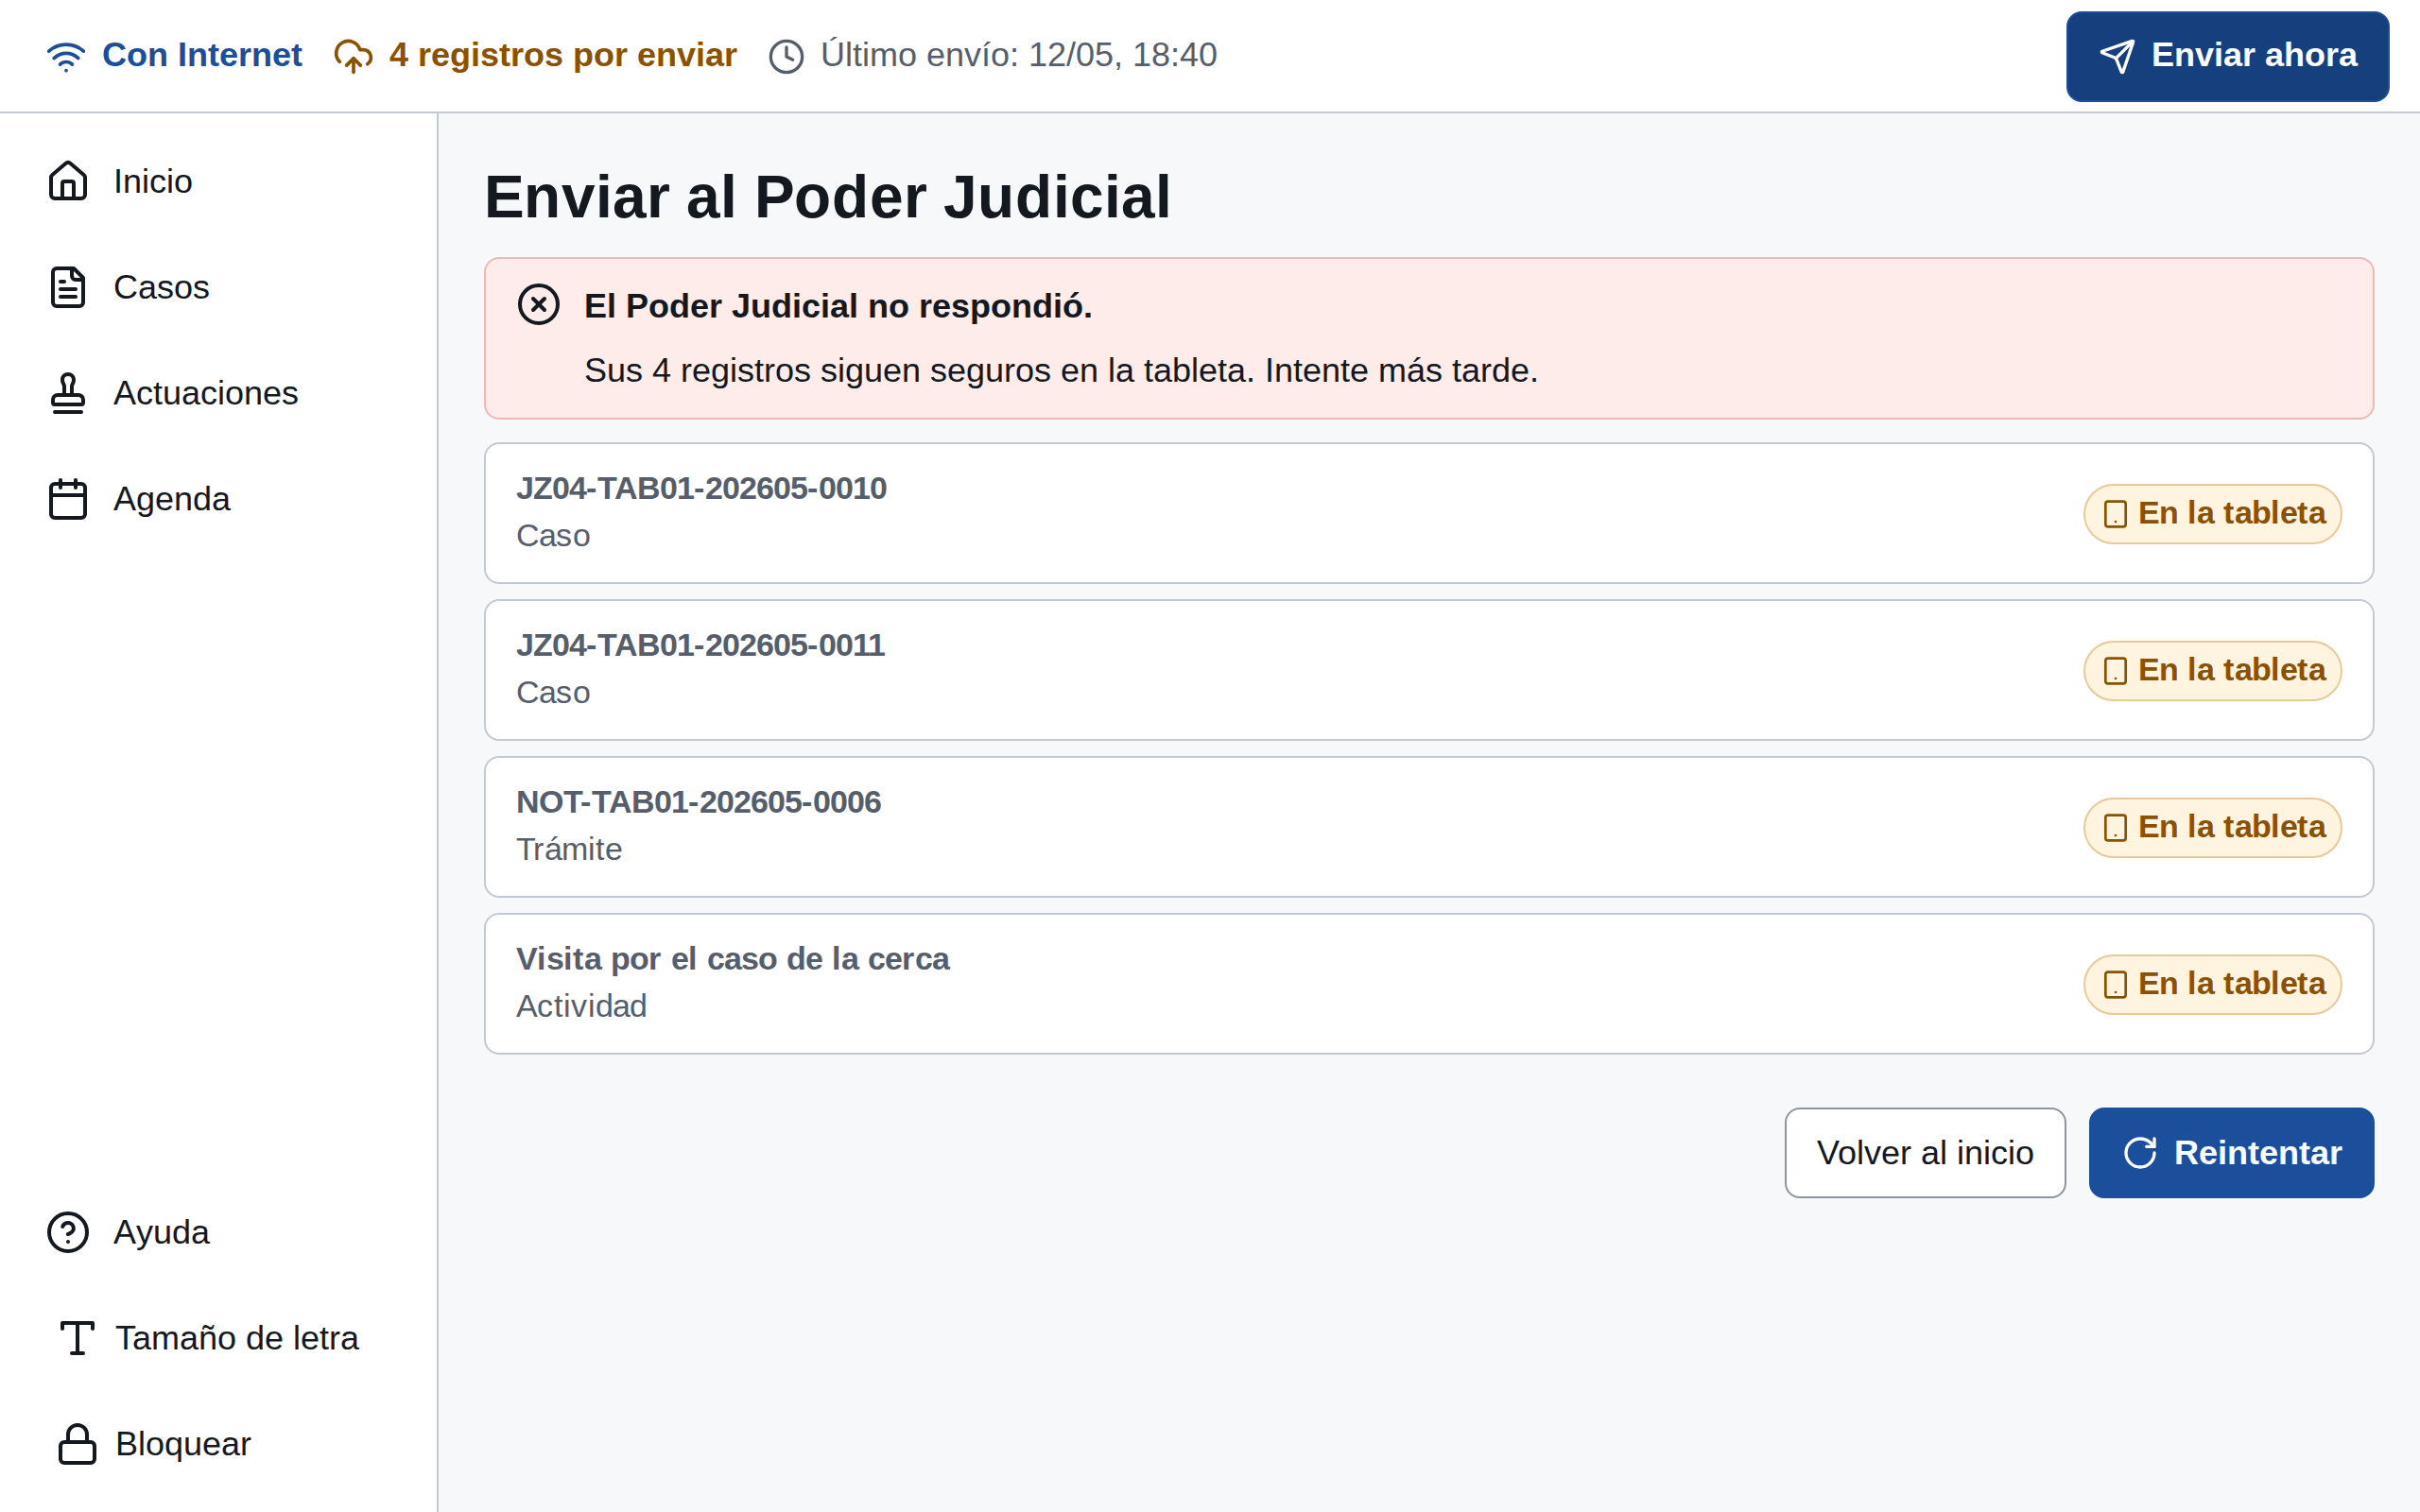
\includegraphics[width=0.82\linewidth]{capturas/P-09d_error-servidor.png}
\caption{P-09 · sync-error. El Poder Judicial no respondió: los registros siguen seguros en la tableta}
\end{figure}
\begin{figure}[H]\centering
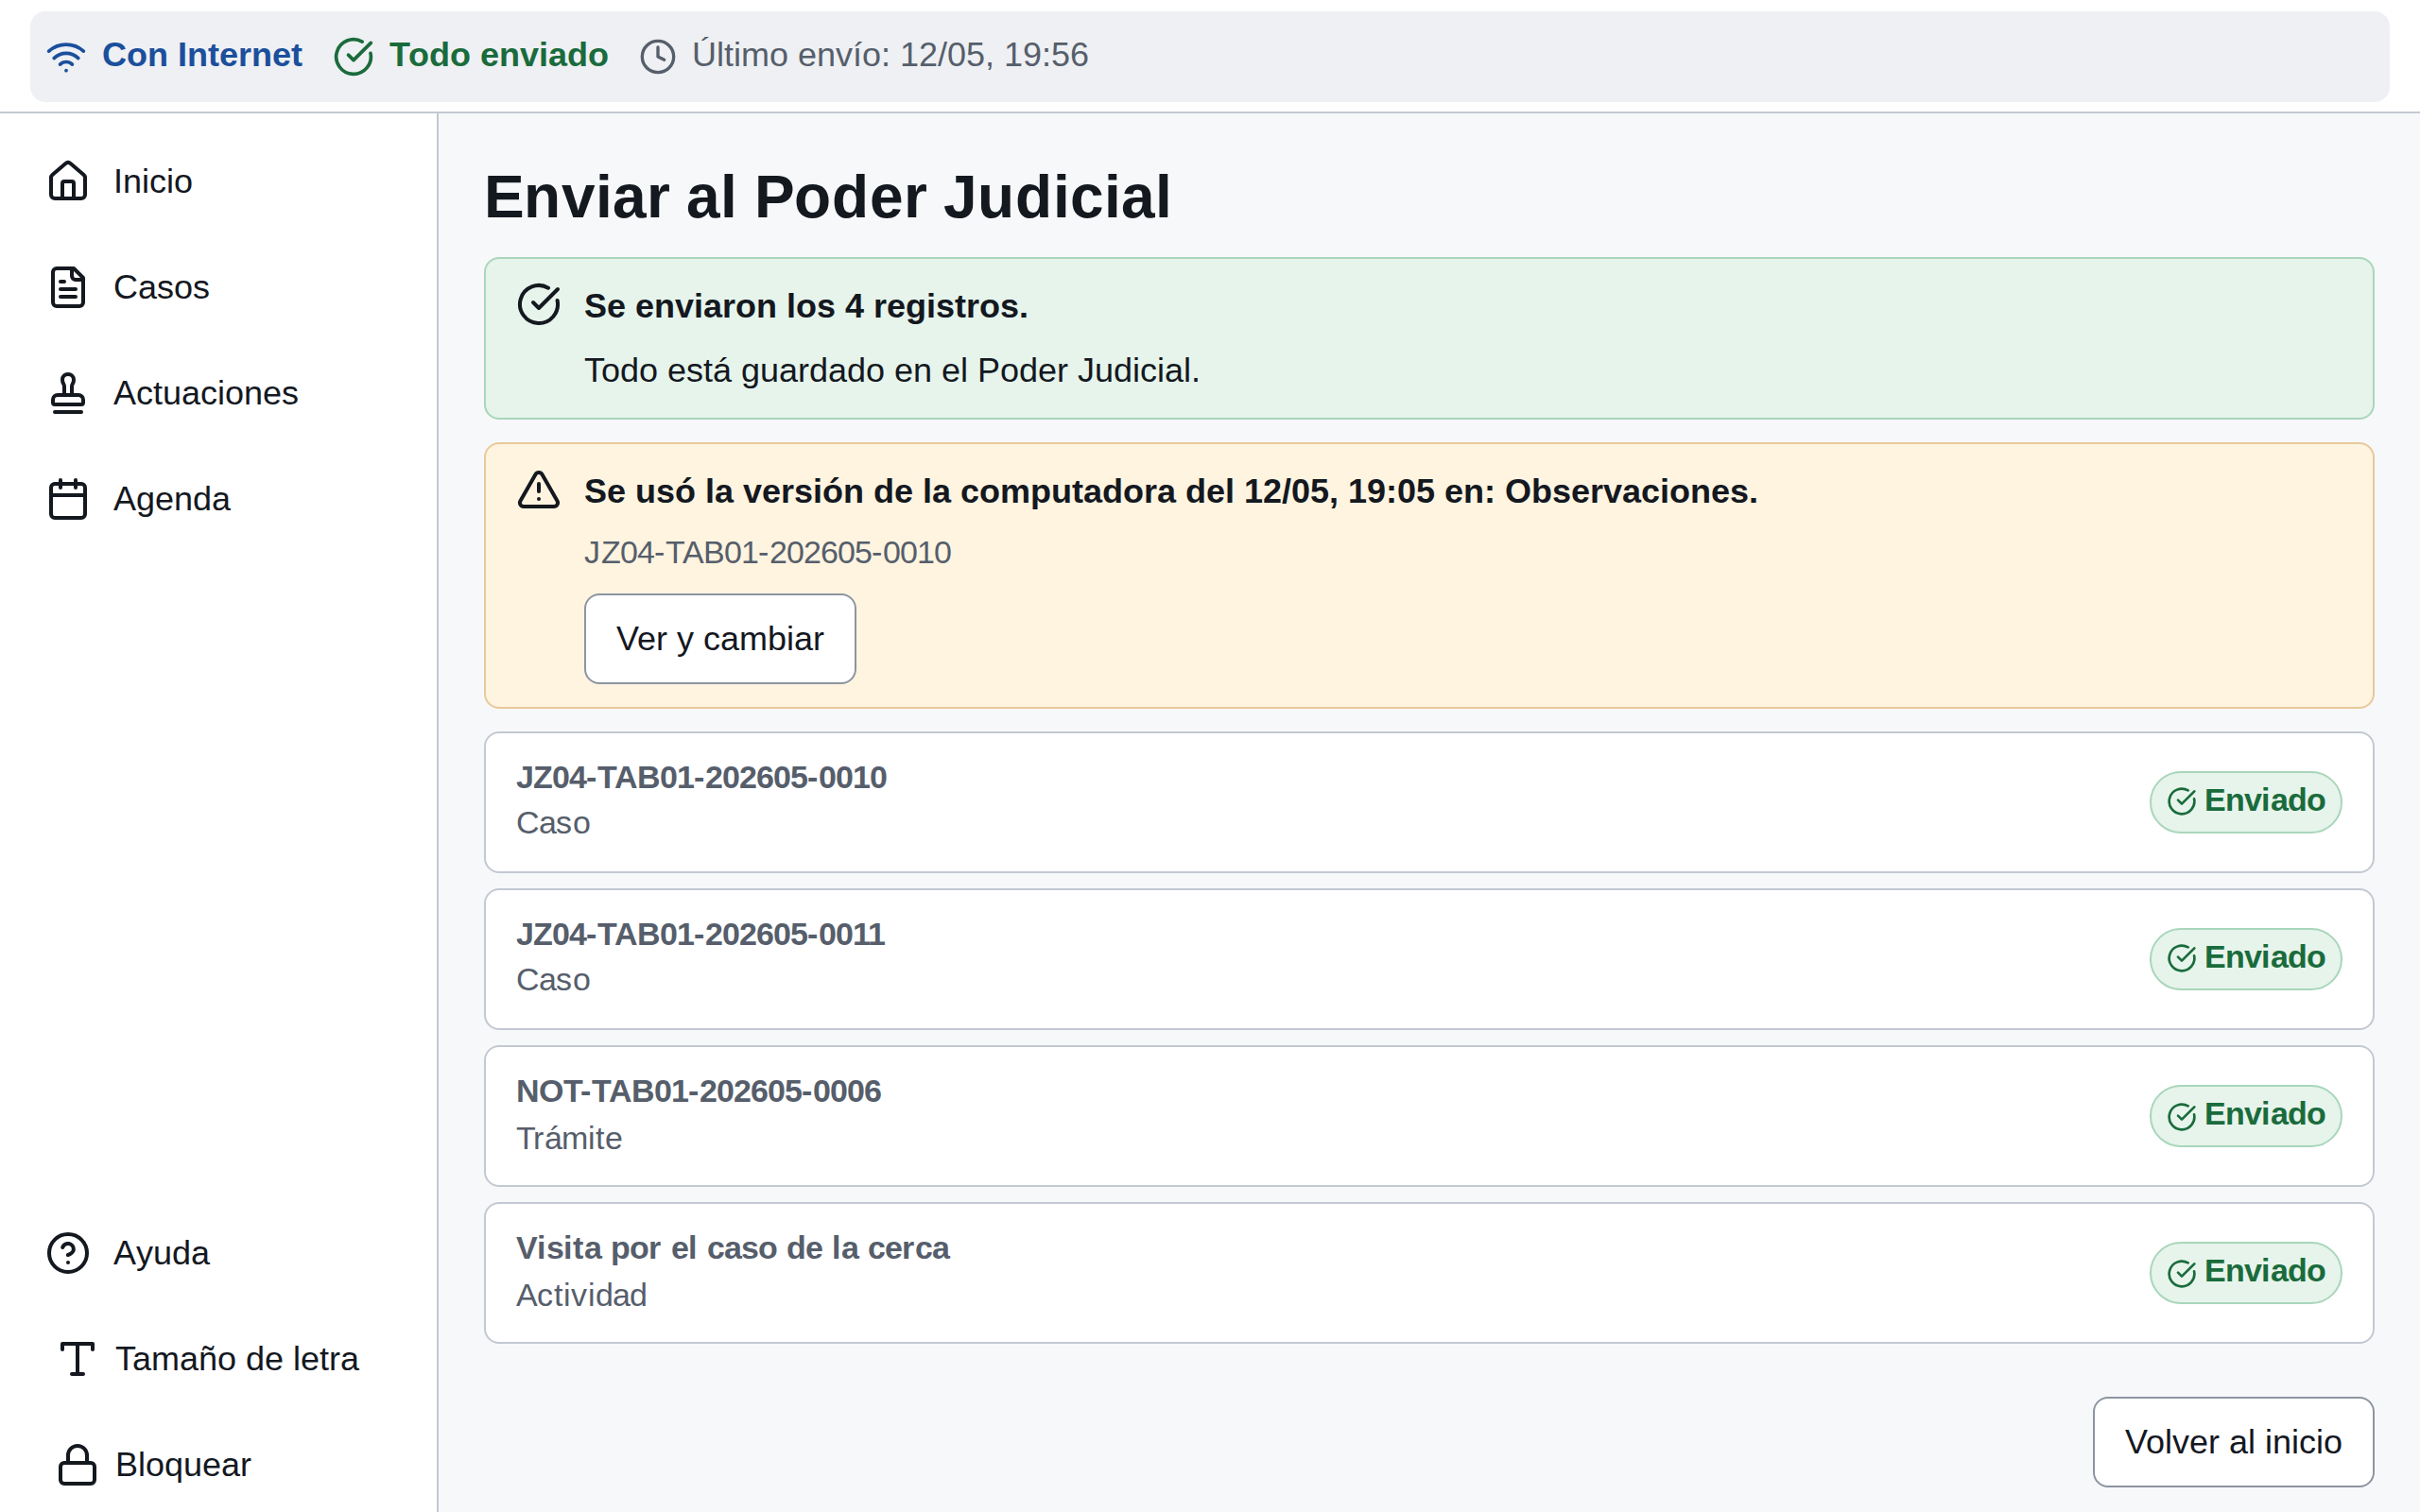
\includegraphics[width=0.82\linewidth]{capturas/P-09e_conflicto.png}
\caption{P-09 · conflict. El conflicto se resuelve solo con el cambio más reciente y se informa qué campo cambió}
\end{figure}
\begin{figure}[H]\centering
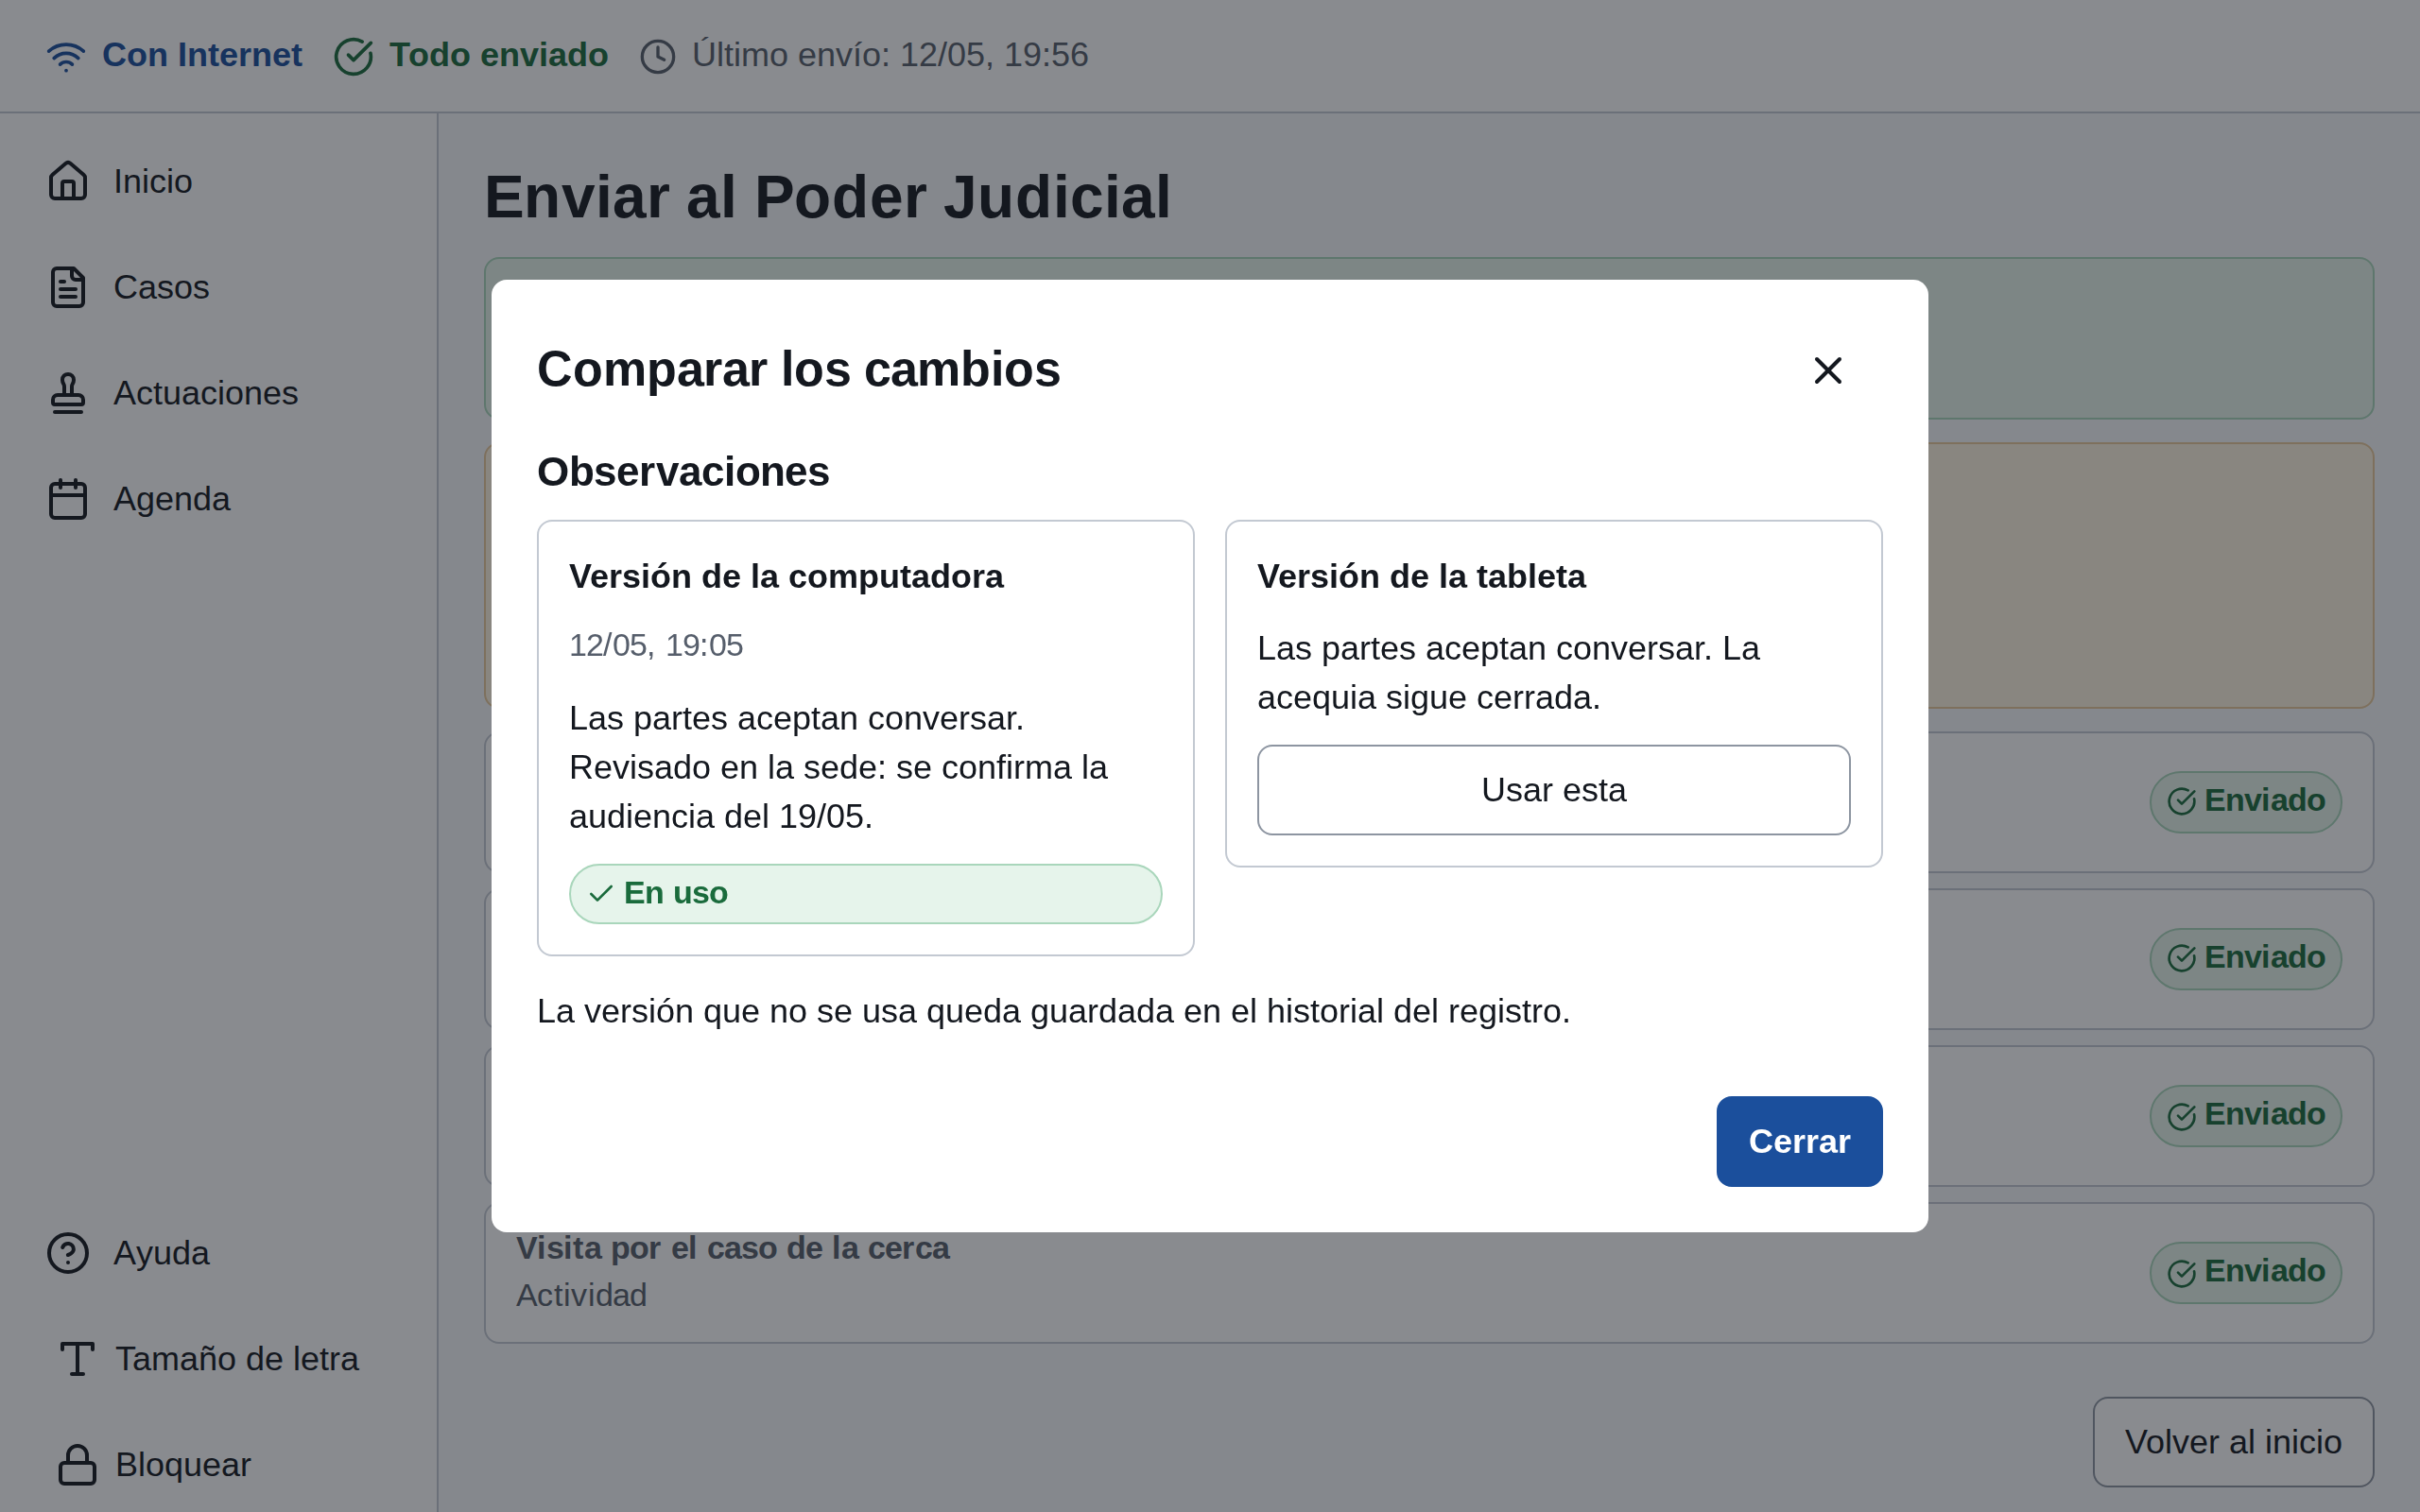
\includegraphics[width=0.82\linewidth]{capturas/P-09f_ver-y-cambiar.png}
\caption{P-09 · Comparación por campo. La comparación campo por campo queda disponible, pero no es obligatoria}
\end{figure}


\section{Los flujos de la situación de uso}

Los cuatro flujos son un solo día de trabajo, capturado en una sola sesión y sin restablecer los datos entre uno y otro. Por eso el contador de la barra encadena: sube a 2 al guardar el caso y su audiencia, a 3 con el trámite y a 4 con la reunión, y al final se envían esos mismos cuatro registros. Los flujos complementarios A y B se capturan aparte.

\subsection{Flujo 1 · Registrar un conflicto vecinal, con corte de conexión a mitad}
\begin{figure}[H]\centering
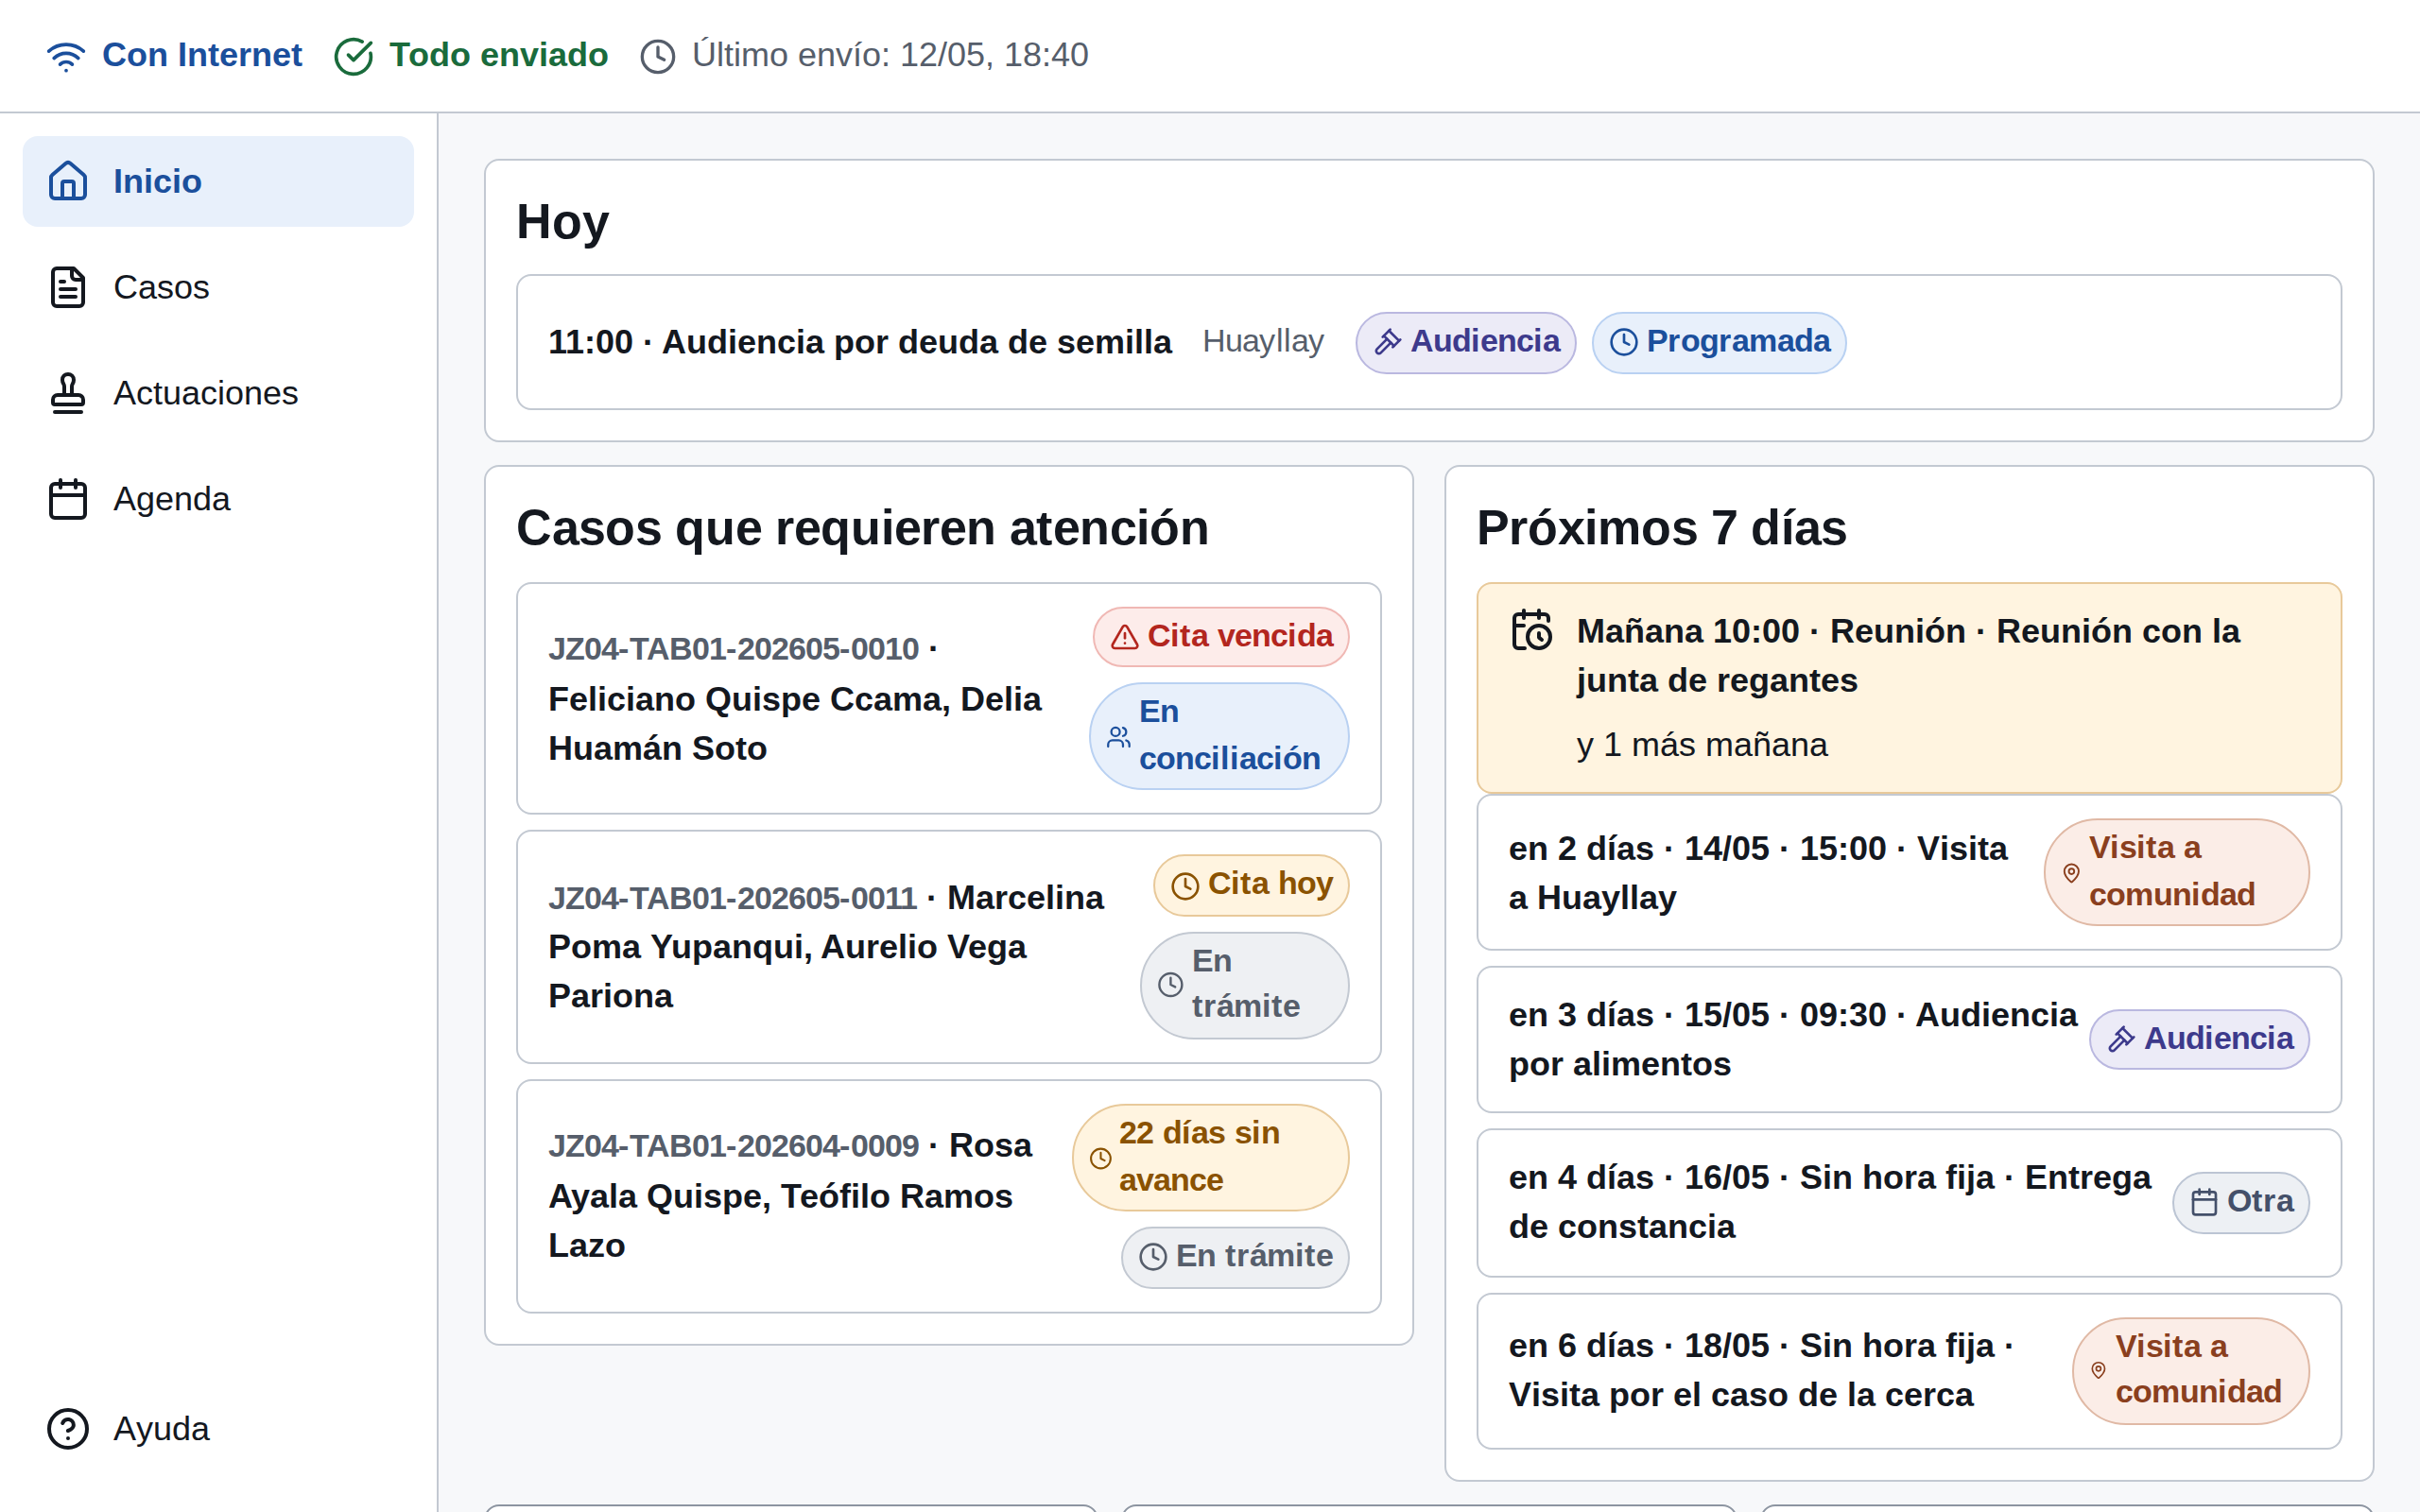
\includegraphics[width=0.82\linewidth]{capturas/F1-01_inicio.png}
\caption{P-01 · 1. Inicio con Internet y todo enviado. Punto de partida: barra en Con Internet y Todo enviado}
\end{figure}
\begin{figure}[H]\centering
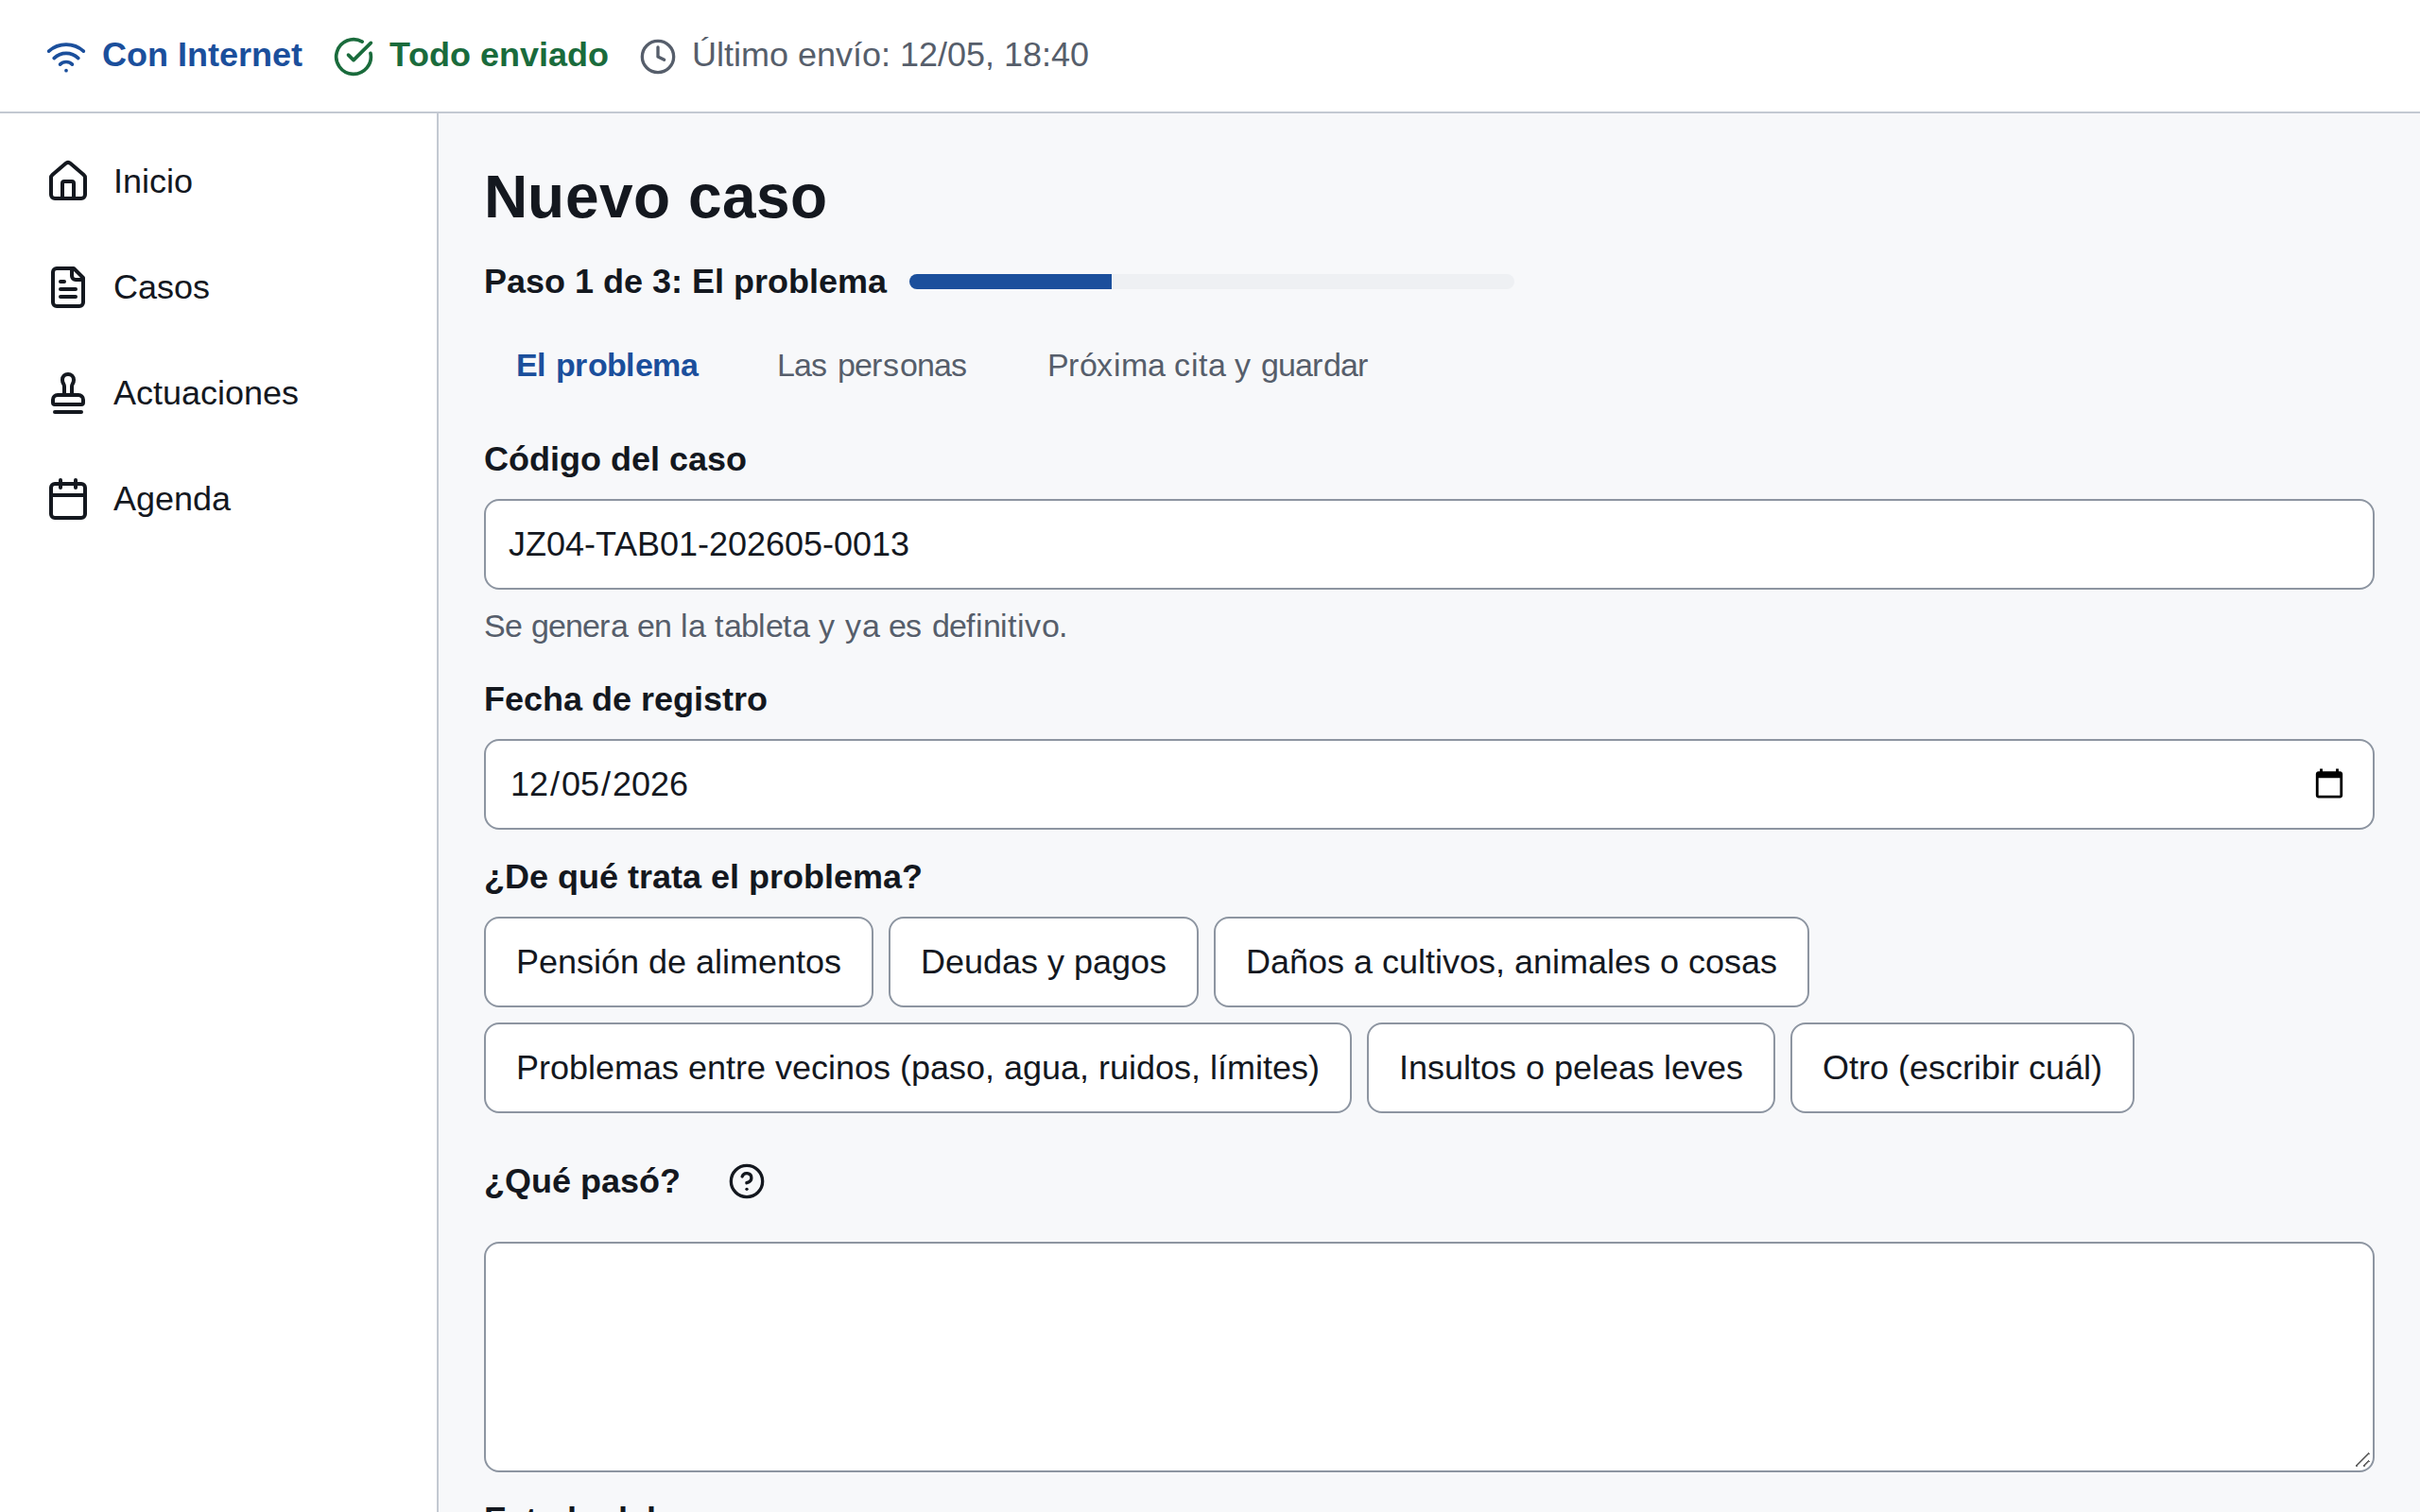
\includegraphics[width=0.82\linewidth]{capturas/F1-02_caso-paso1.png}
\caption{P-03 · 2. Paso 1, el problema. Código generado en la tableta y catálogo de tipos de problema en botones grandes}
\end{figure}
\begin{figure}[H]\centering
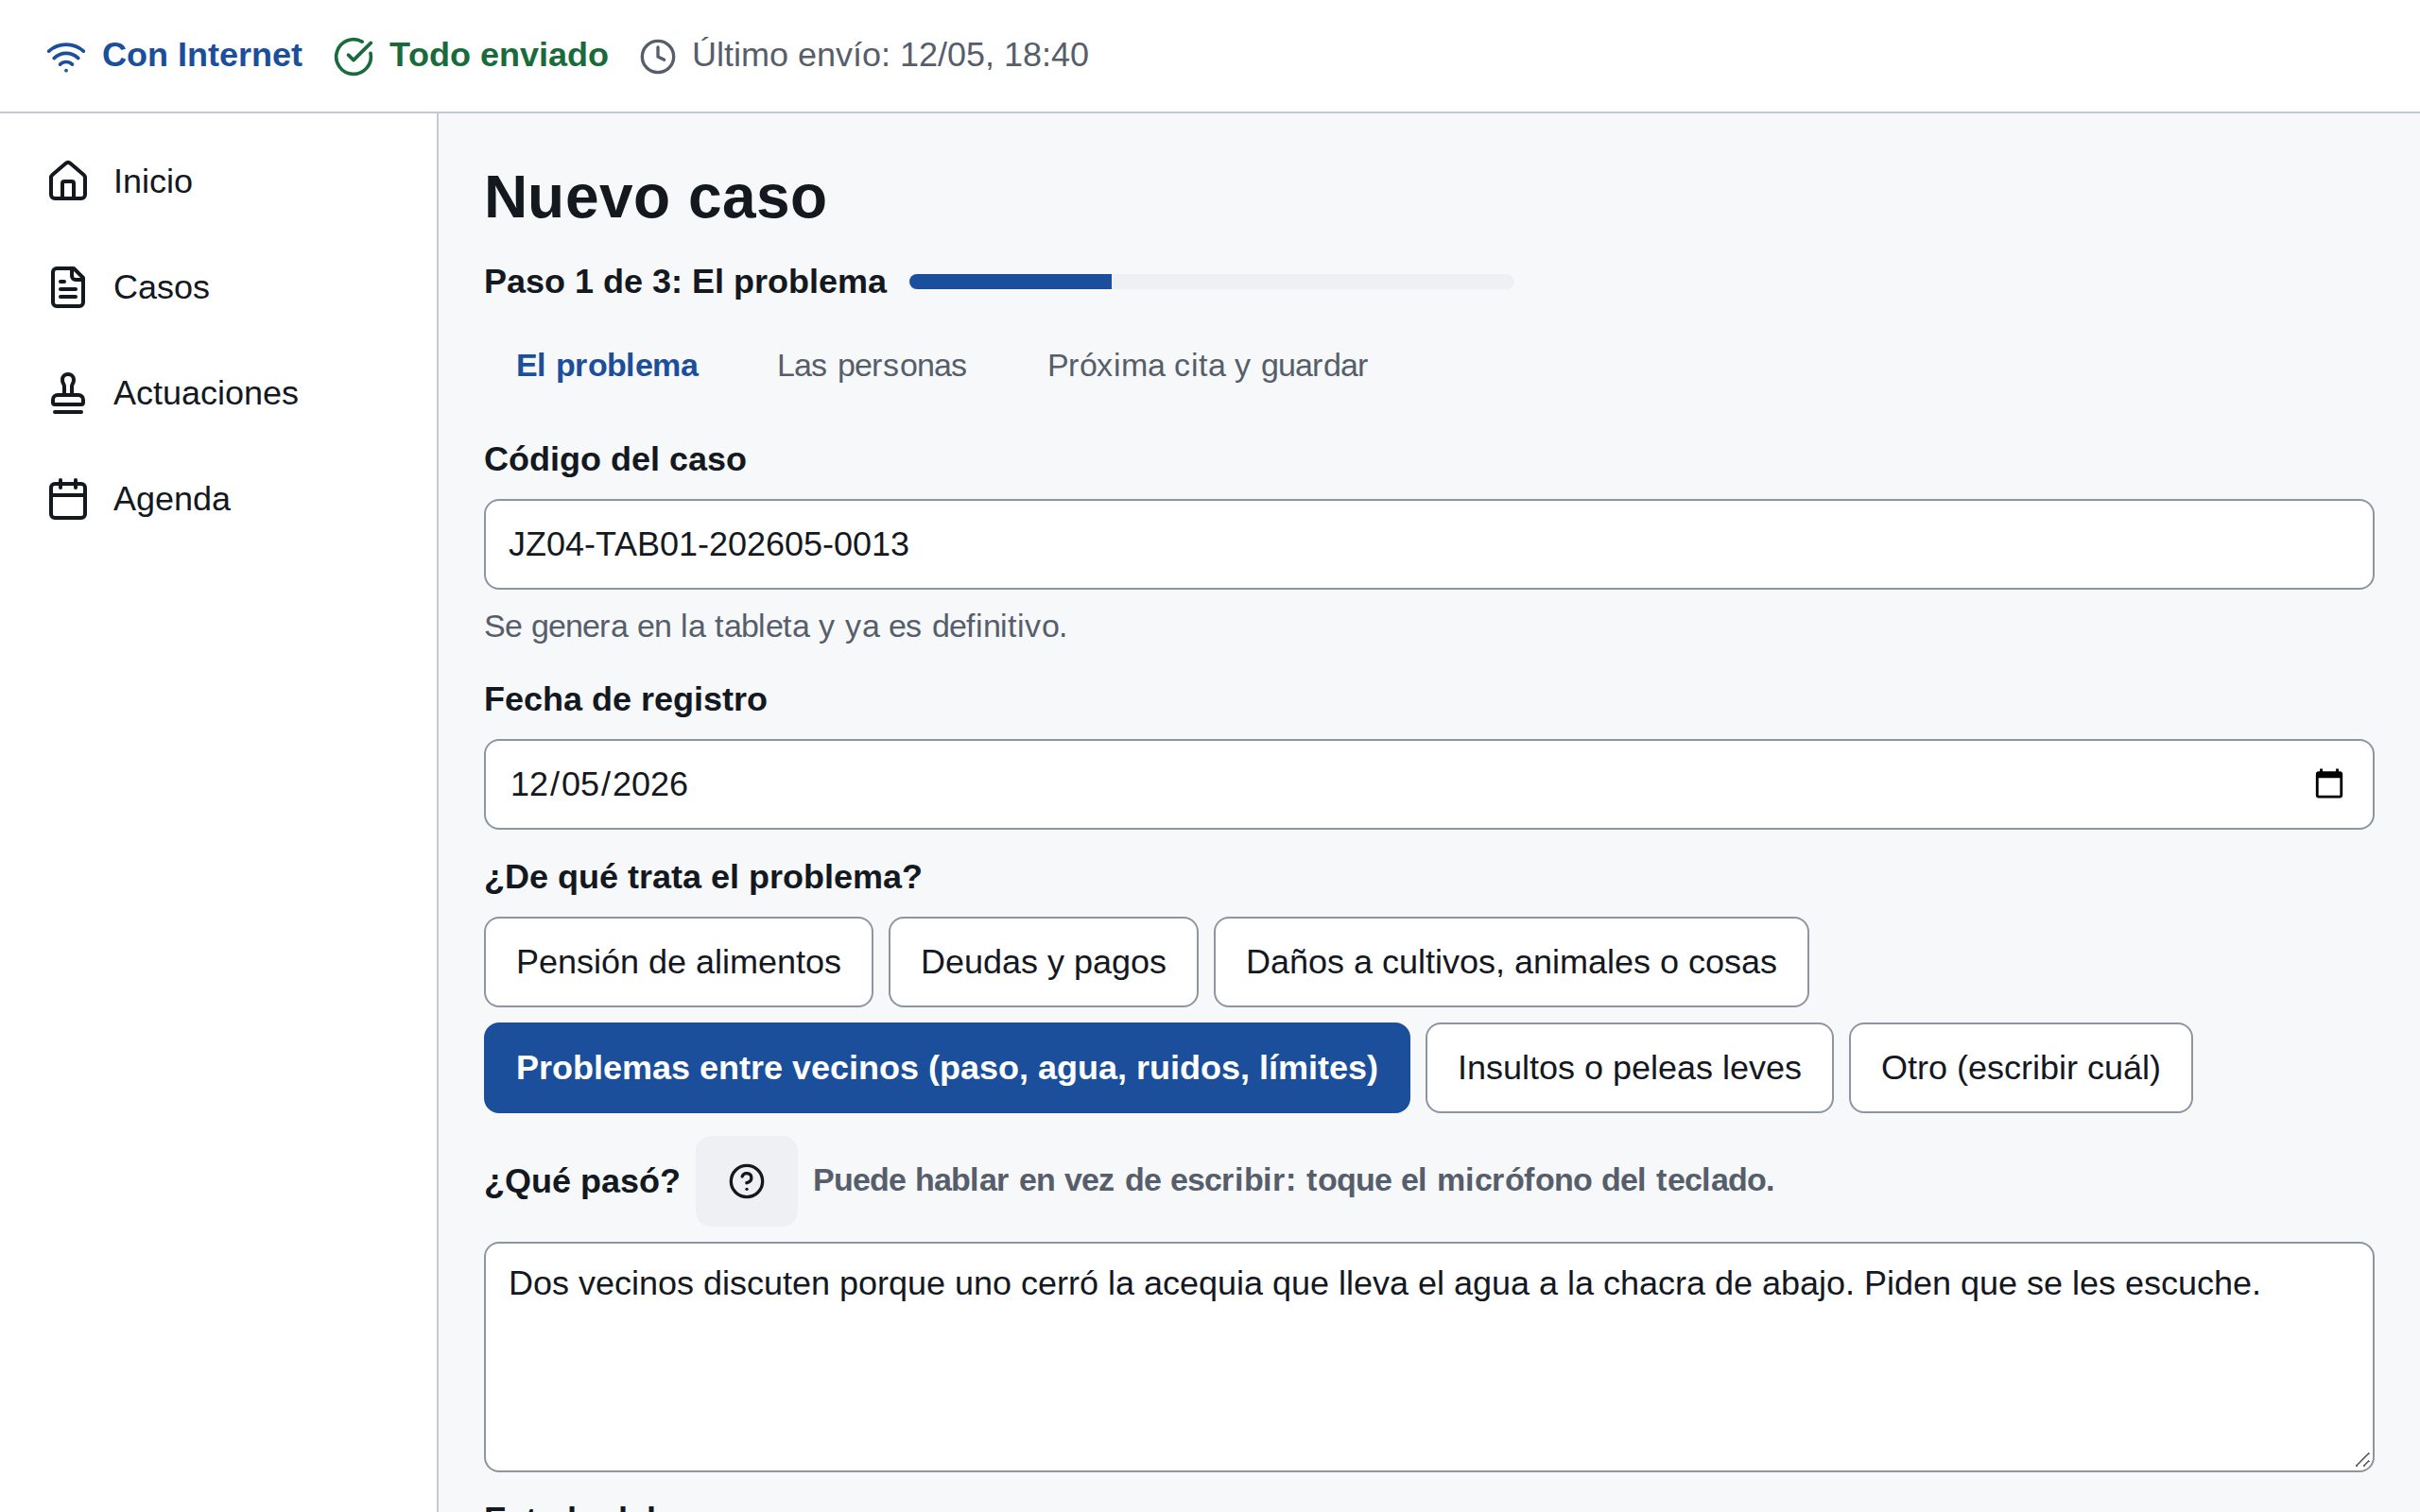
\includegraphics[width=0.82\linewidth]{capturas/F1-03_caso-paso1-lleno.png}
\caption{P-03 · 2. Paso 1 completo. Descripción con la ayuda para dictar desde el teclado, sin micrófono propio}
\end{figure}
\begin{figure}[H]\centering
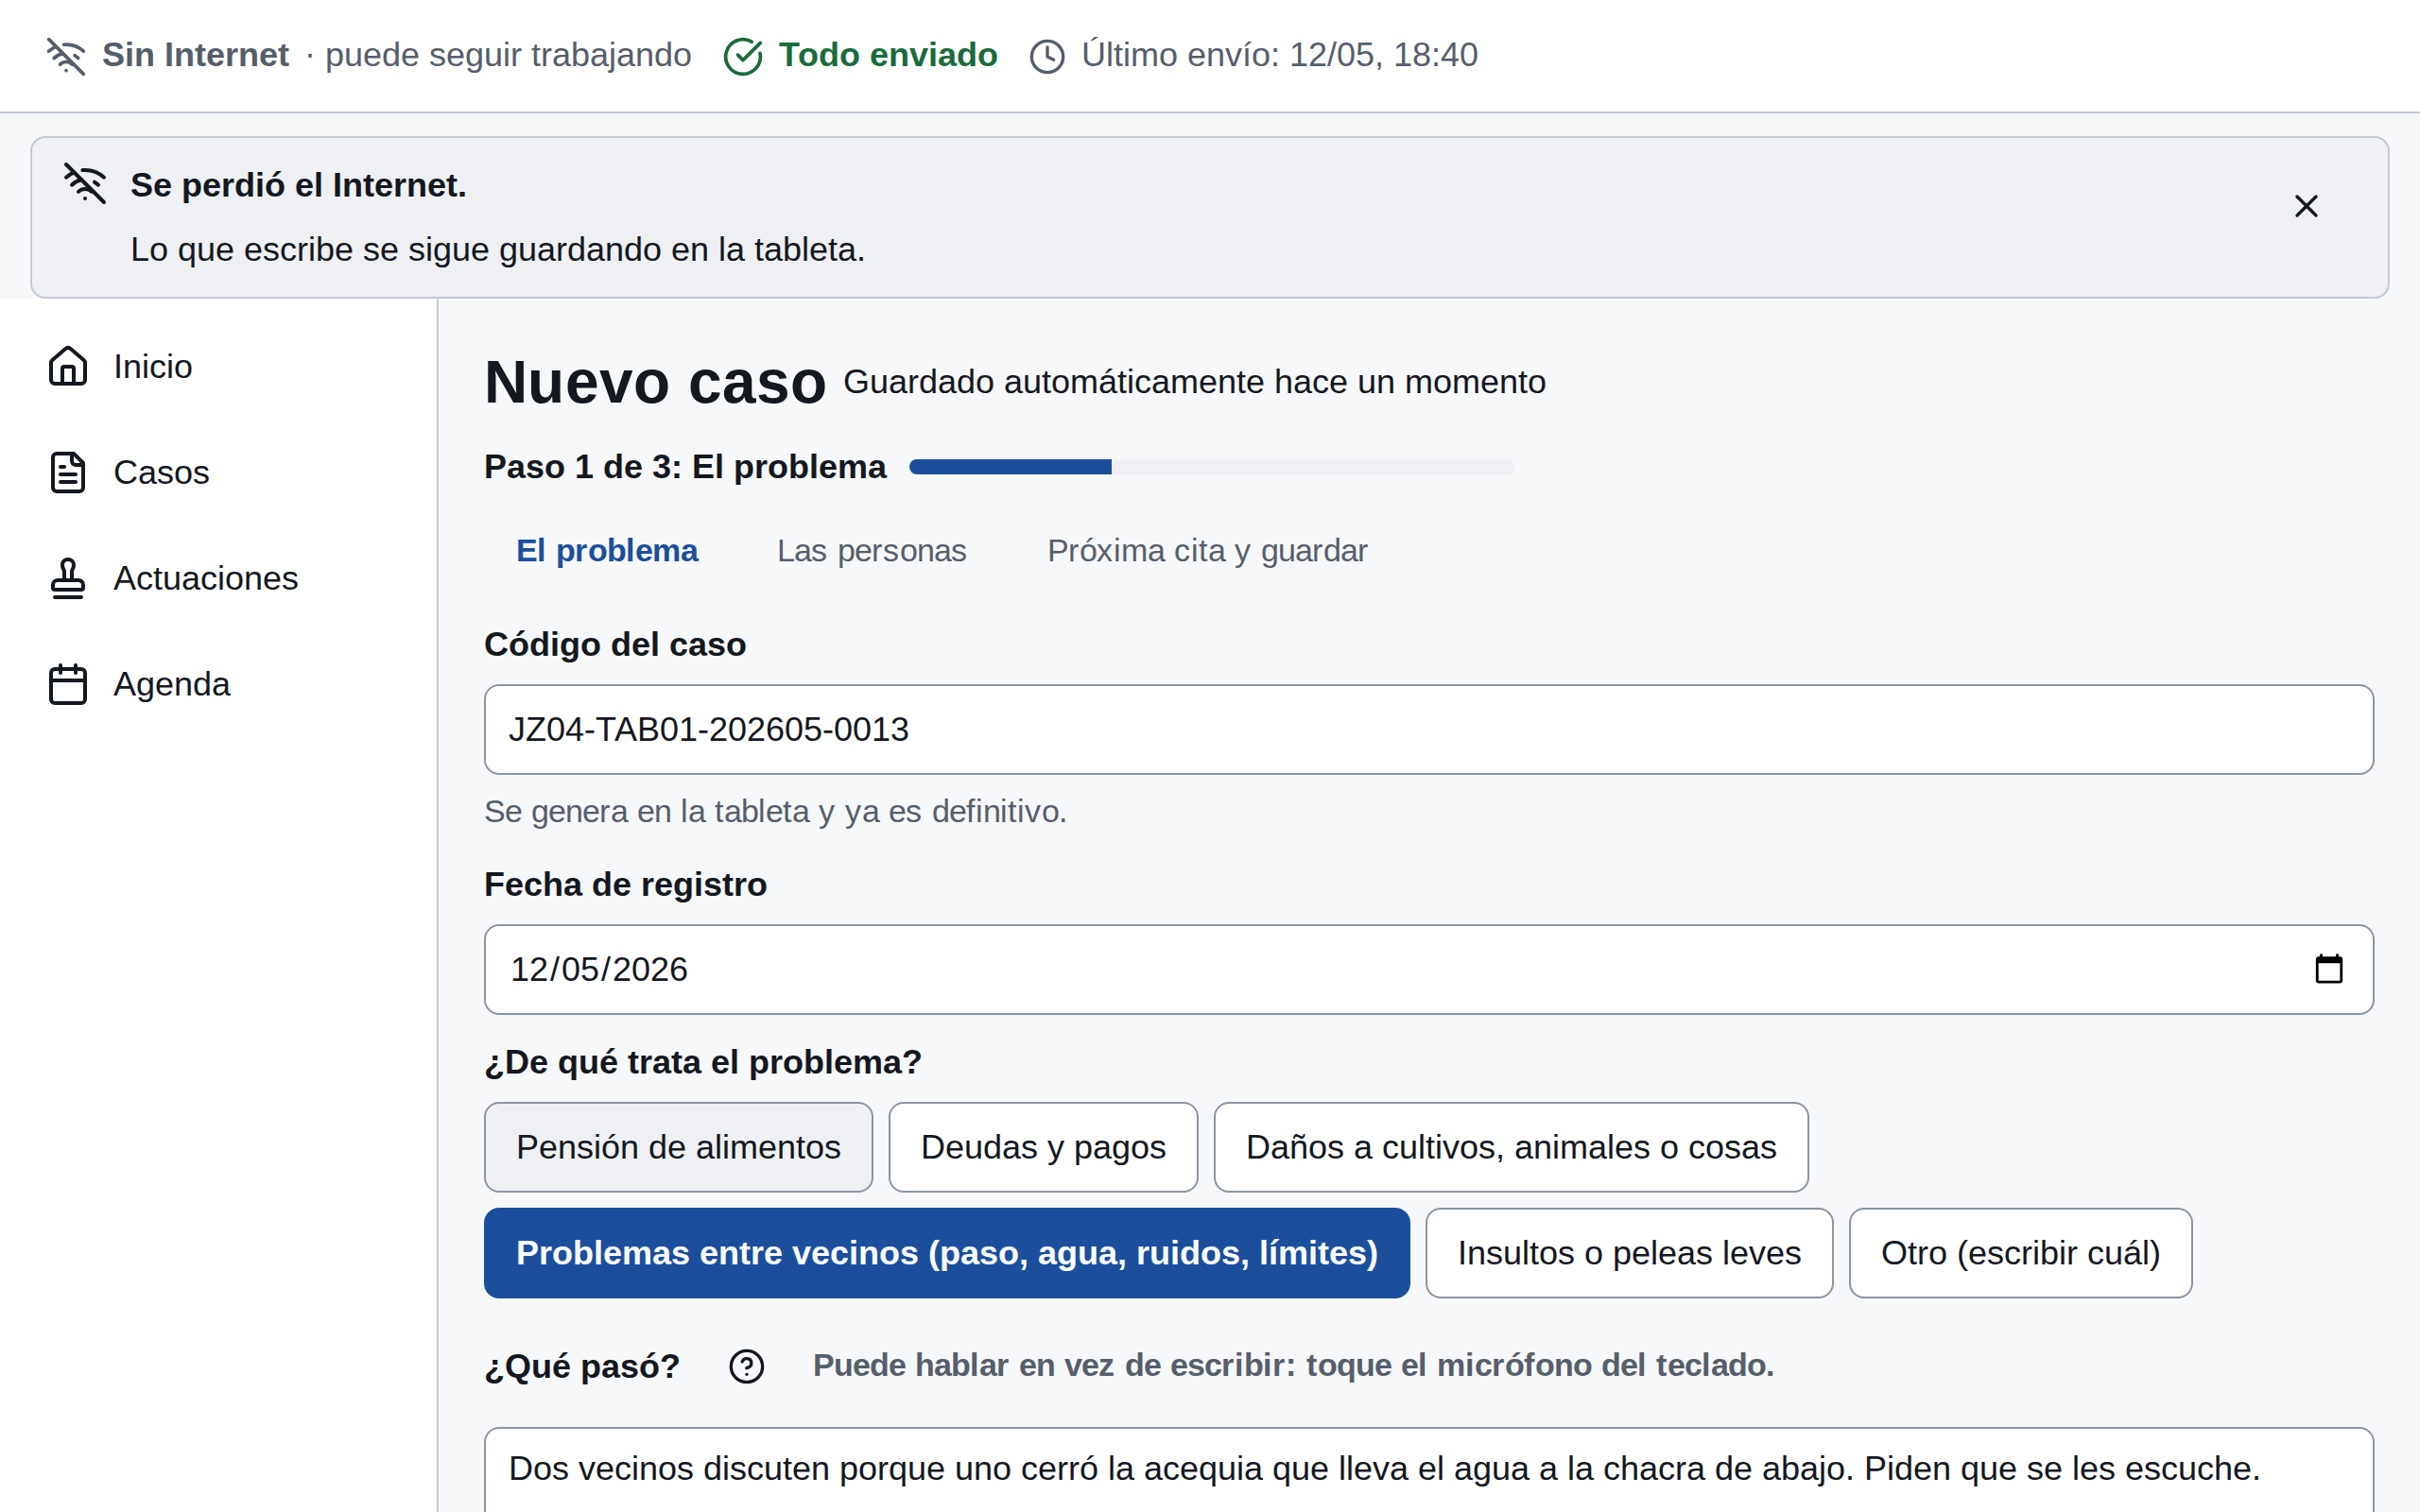
\includegraphics[width=0.82\linewidth]{capturas/F1-04_corte-internet.png}
\caption{P-03 · 3. Se corta el Internet a mitad del formulario. Aviso de corte sin alarma y barra en Sin Internet, en gris; el trabajo continúa}
\end{figure}
\begin{figure}[H]\centering
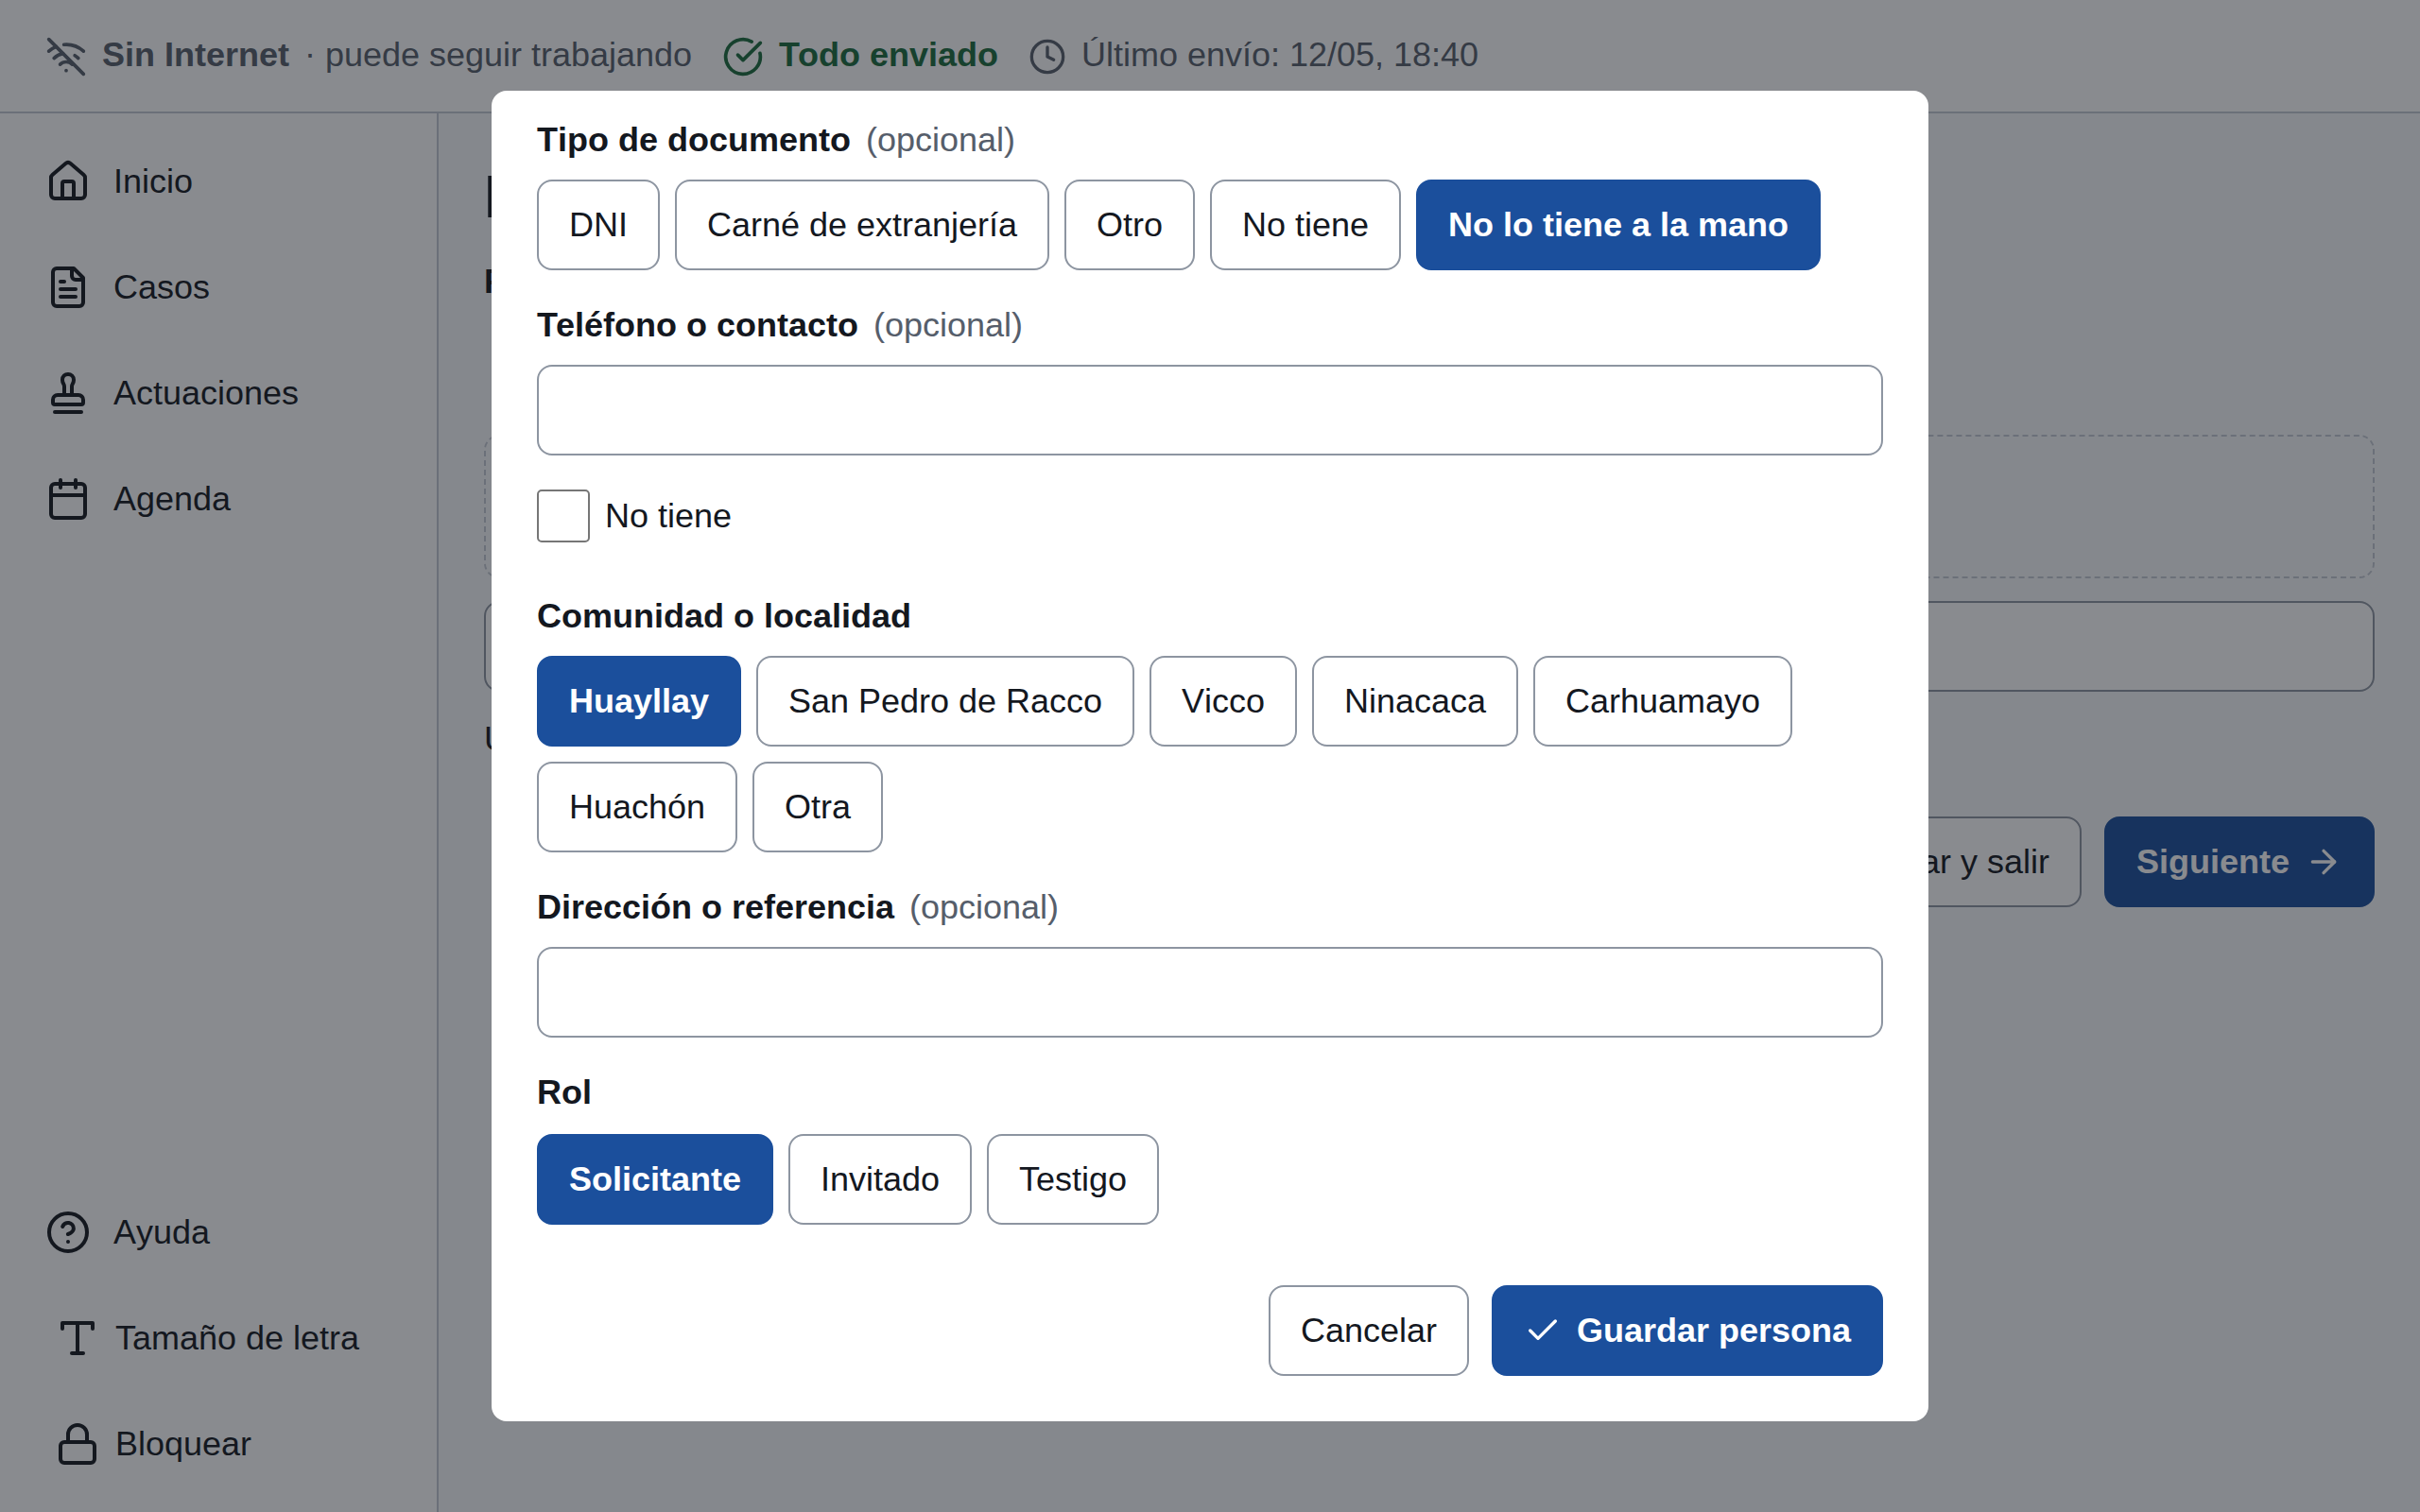
\includegraphics[width=0.82\linewidth]{capturas/F1-05_persona-1.png}
\caption{P-03 · 4. Primera parte, sin documento a la mano. Opción No lo tiene a la mano en vez de obligar un DNI inventado}
\end{figure}
\begin{figure}[H]\centering
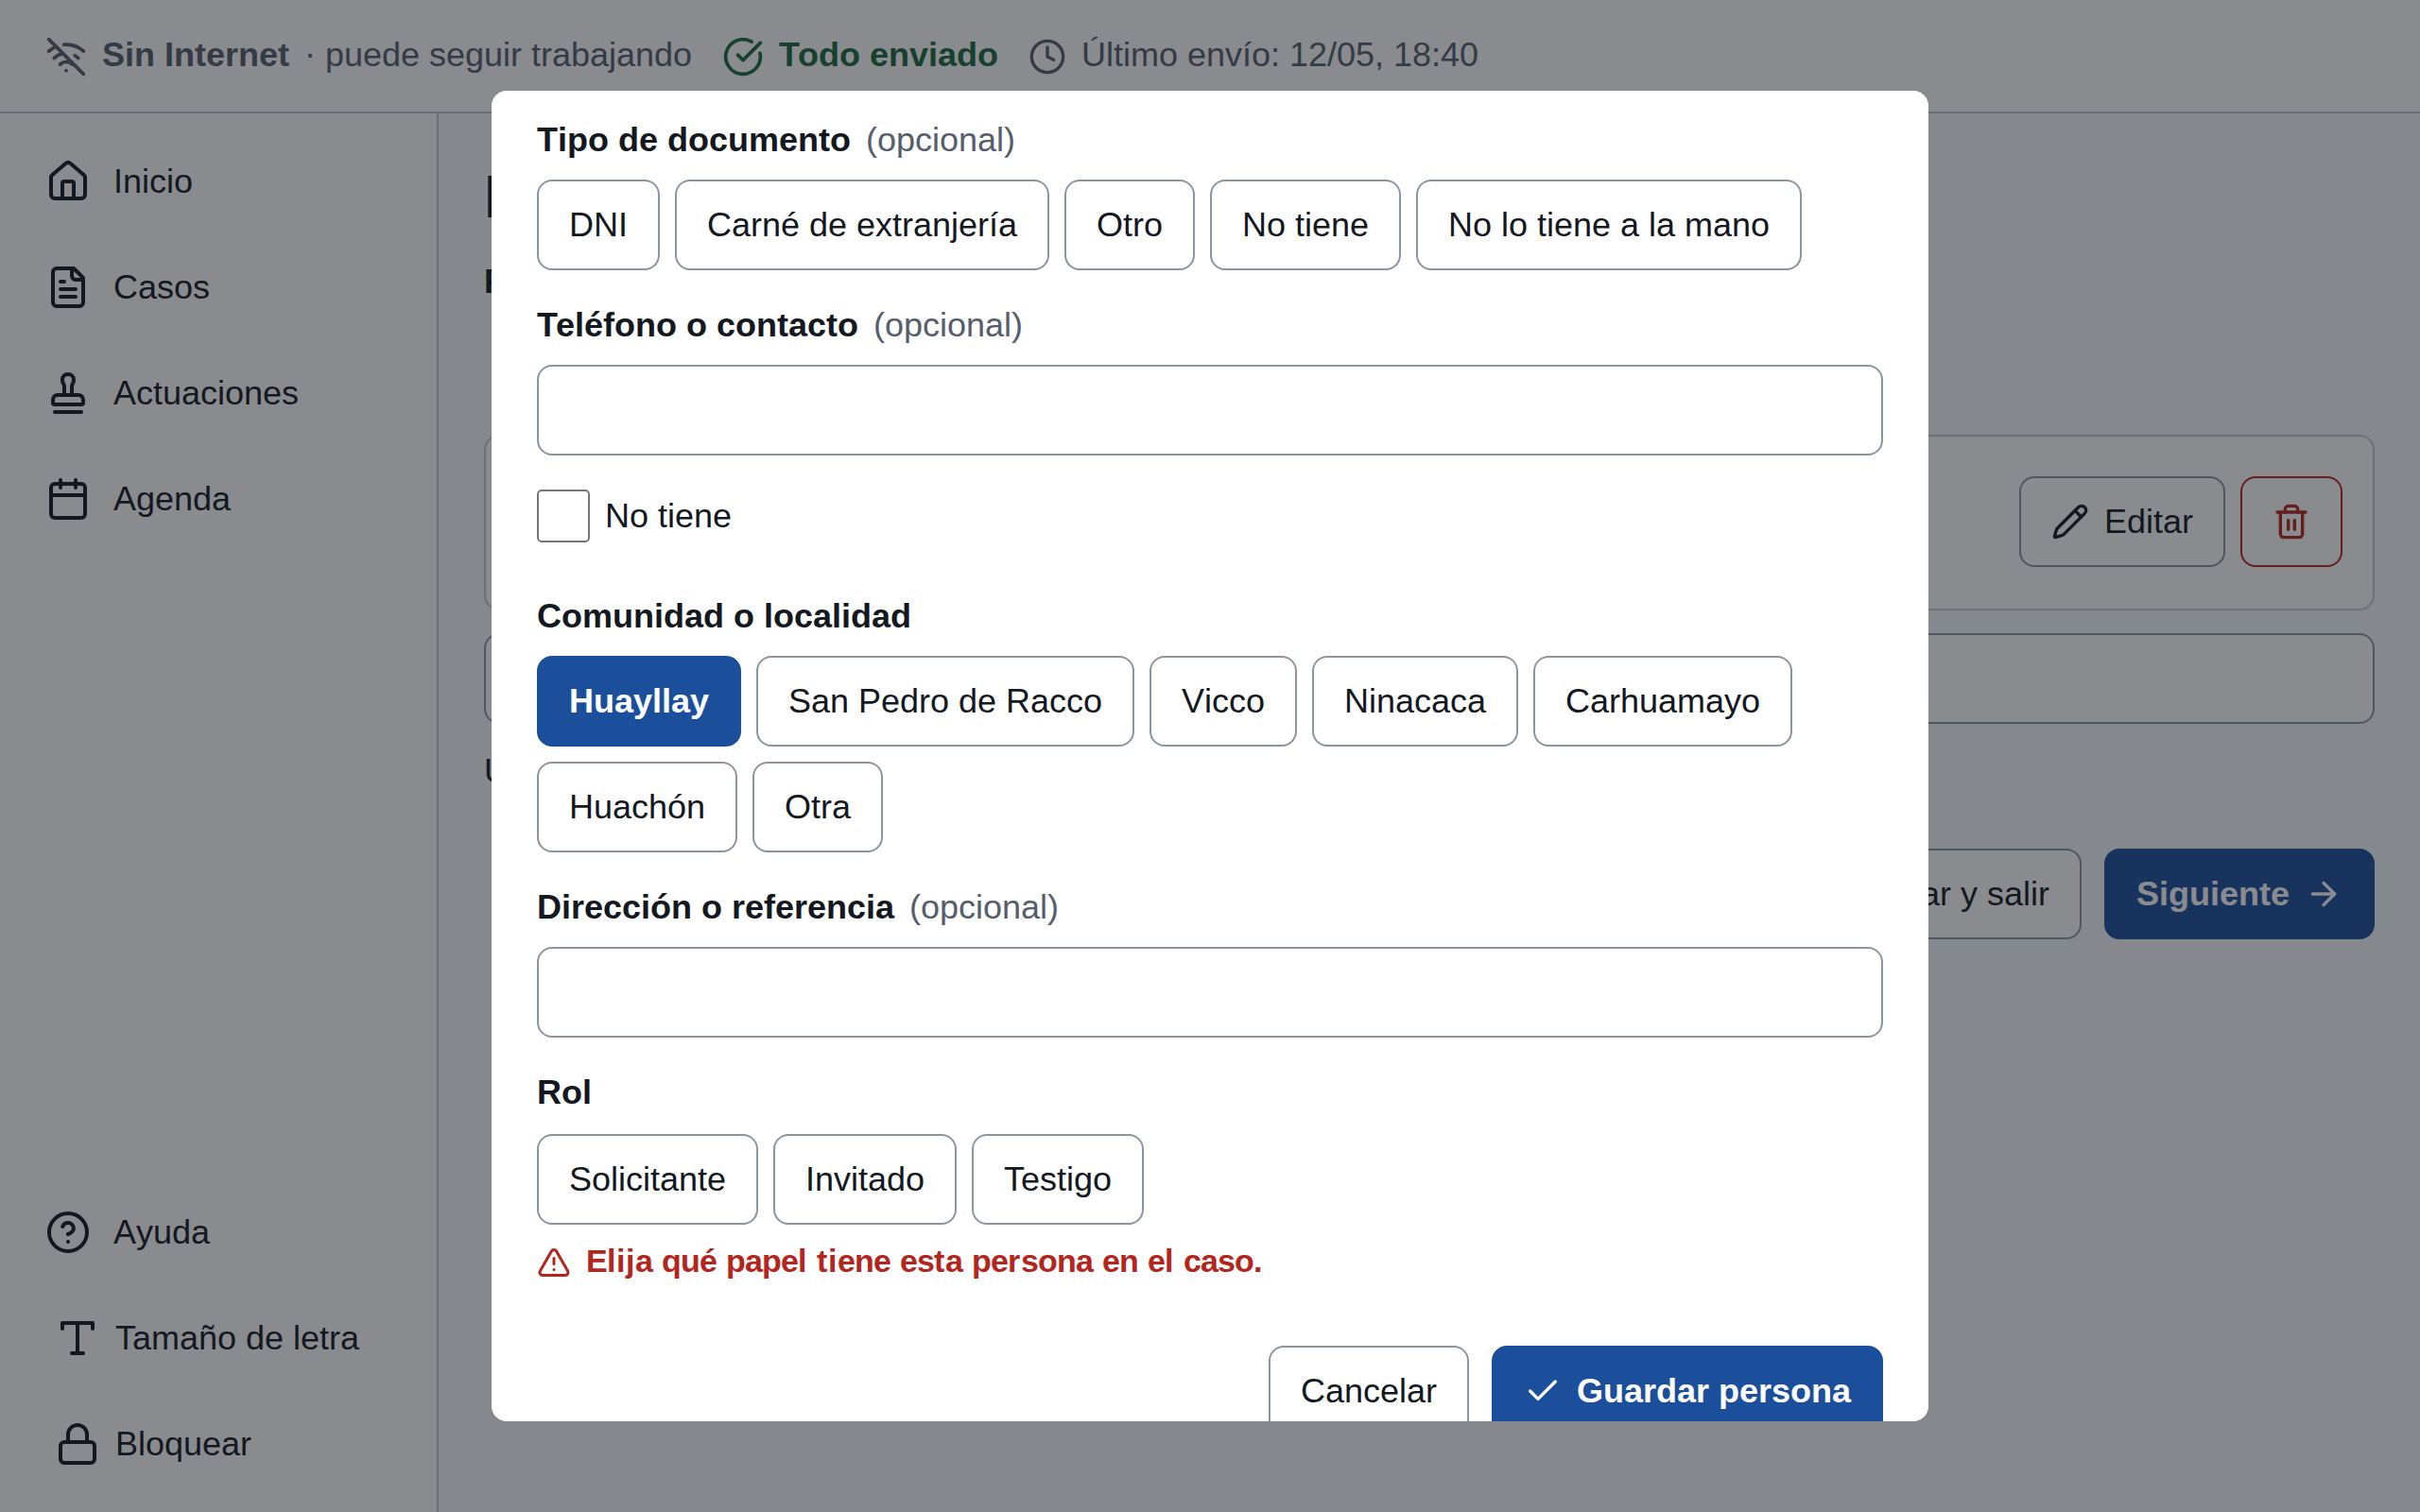
\includegraphics[width=0.82\linewidth]{capturas/F1-06_error-rol.png}
\caption{P-03 · 6. Error de validación en lenguaje simple. Mensaje que dice qué falta y cómo resolverlo, sin jerga}
\end{figure}
\begin{figure}[H]\centering
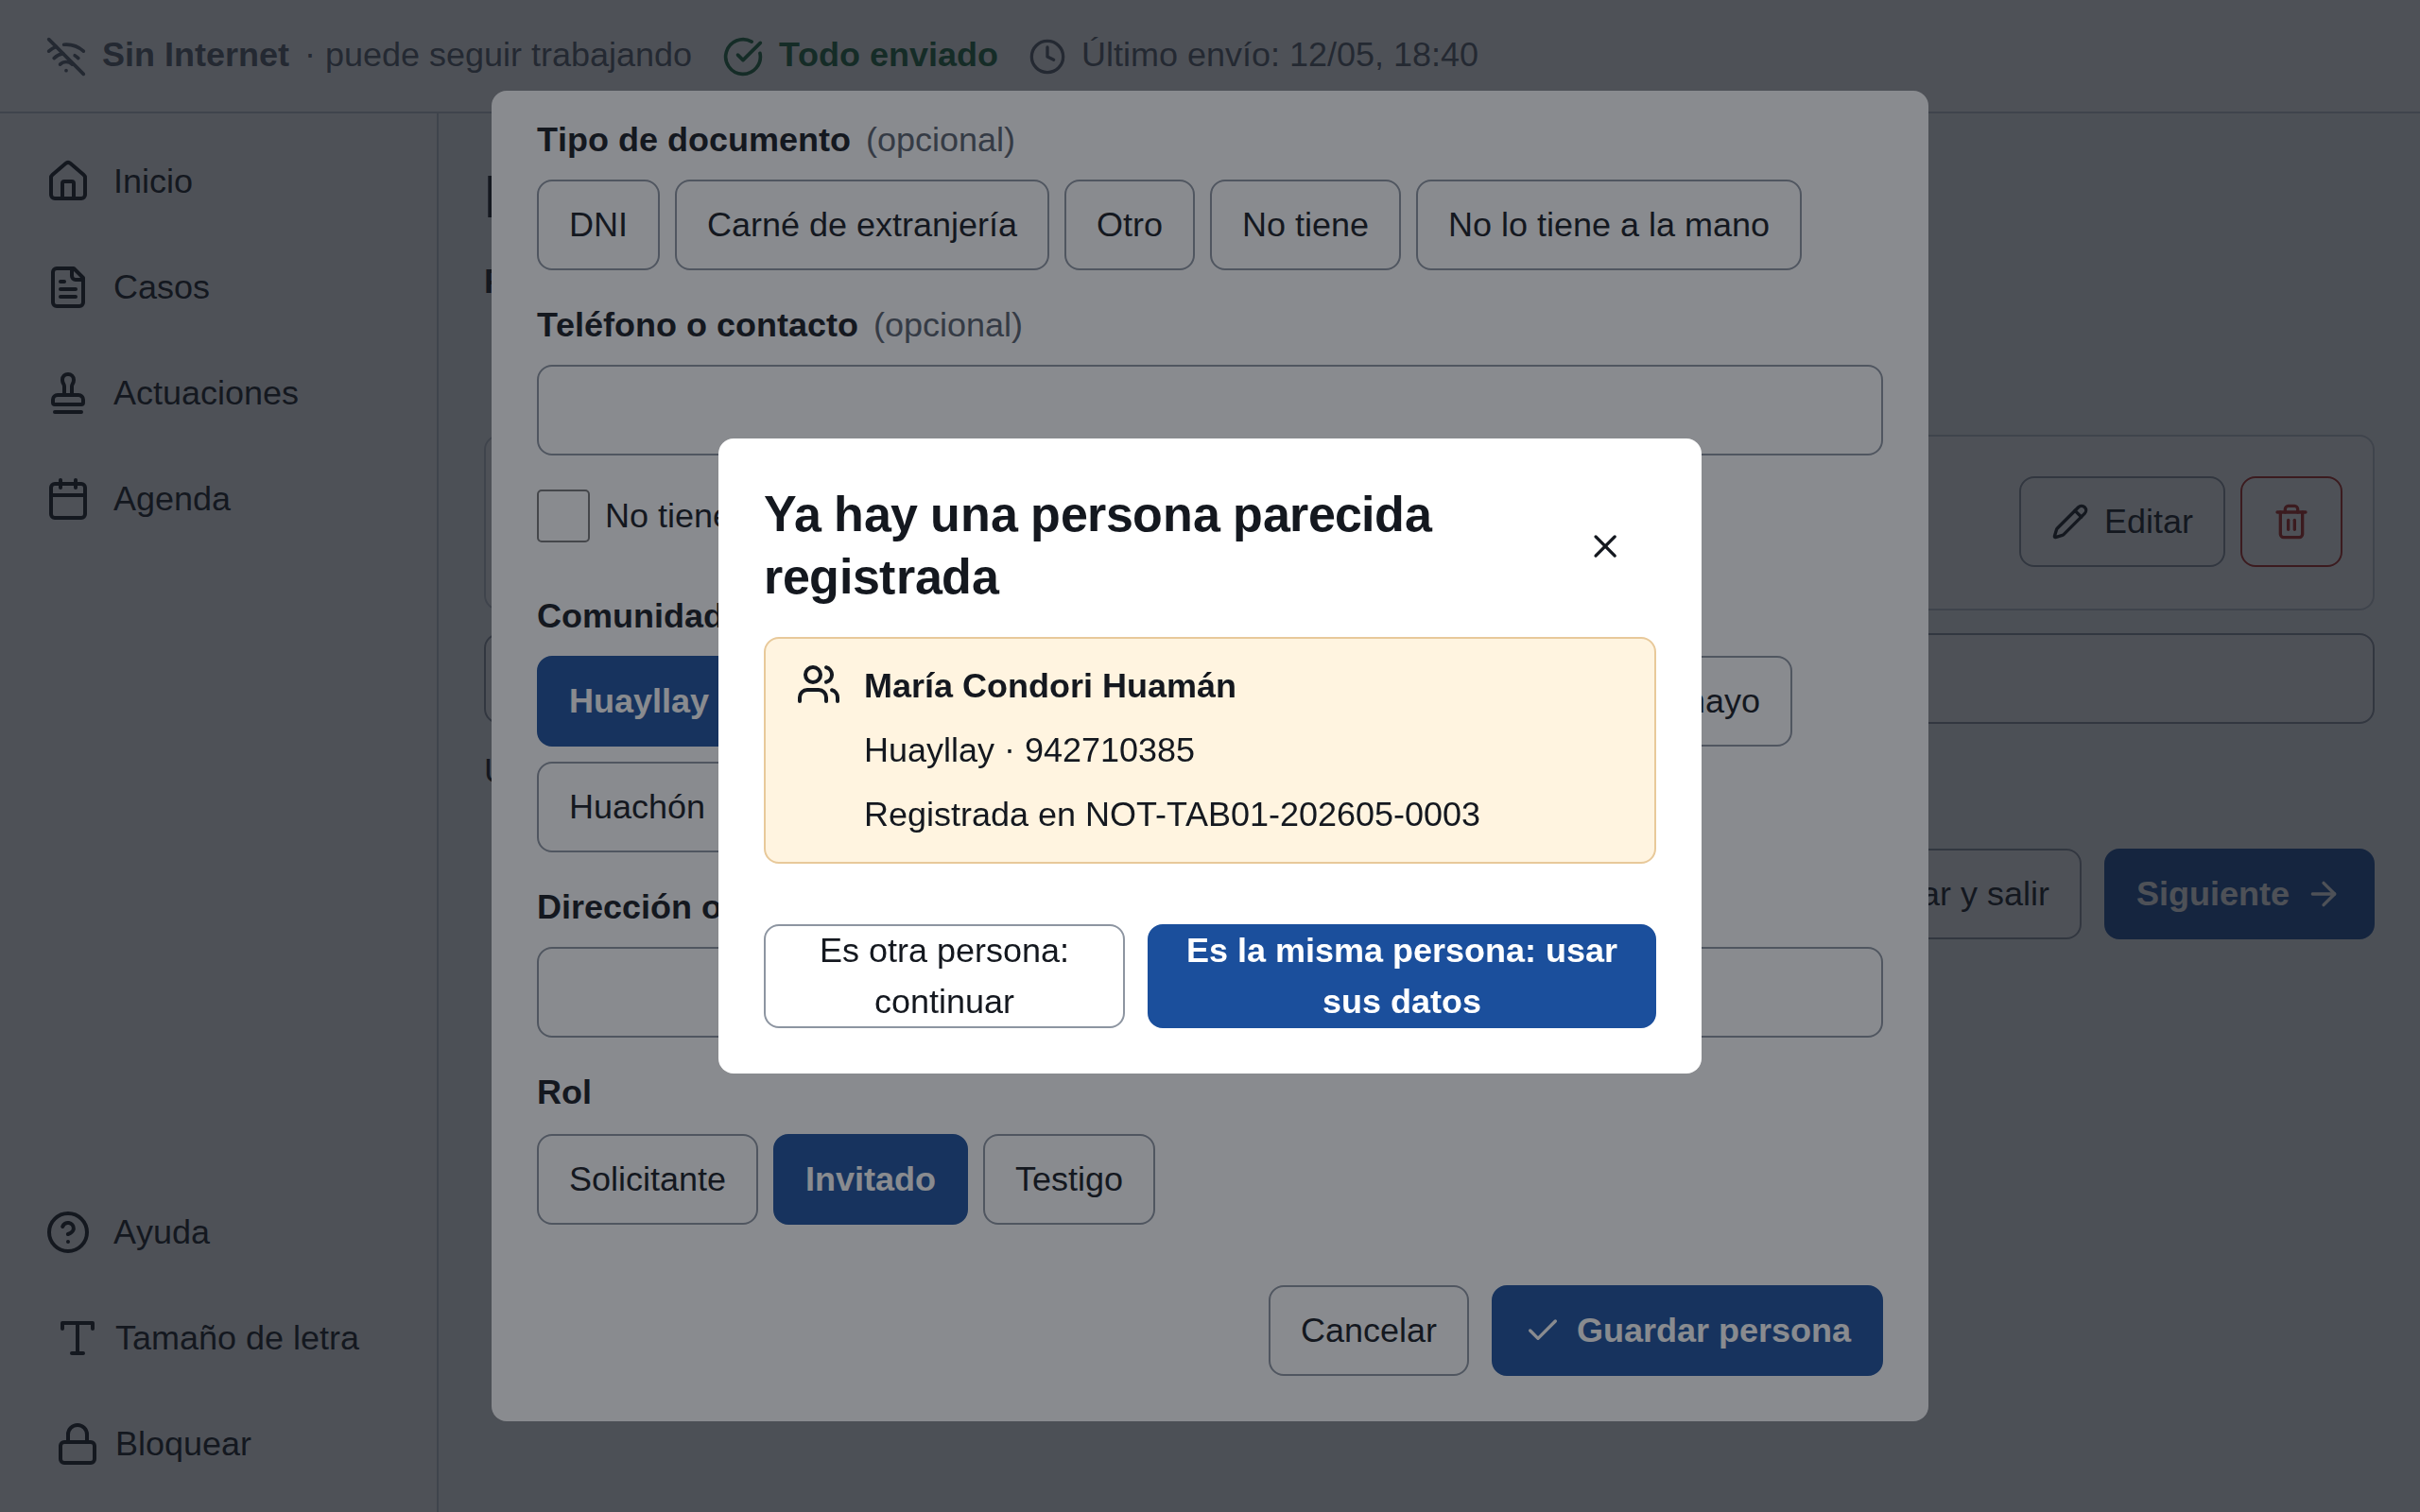
\includegraphics[width=0.82\linewidth]{capturas/F1-07_duplicado.png}
\caption{P-03 · 5. Advertencia de persona duplicada. Advierte sin bloquear y deja elegir entre usar sus datos o continuar}
\end{figure}
\begin{figure}[H]\centering
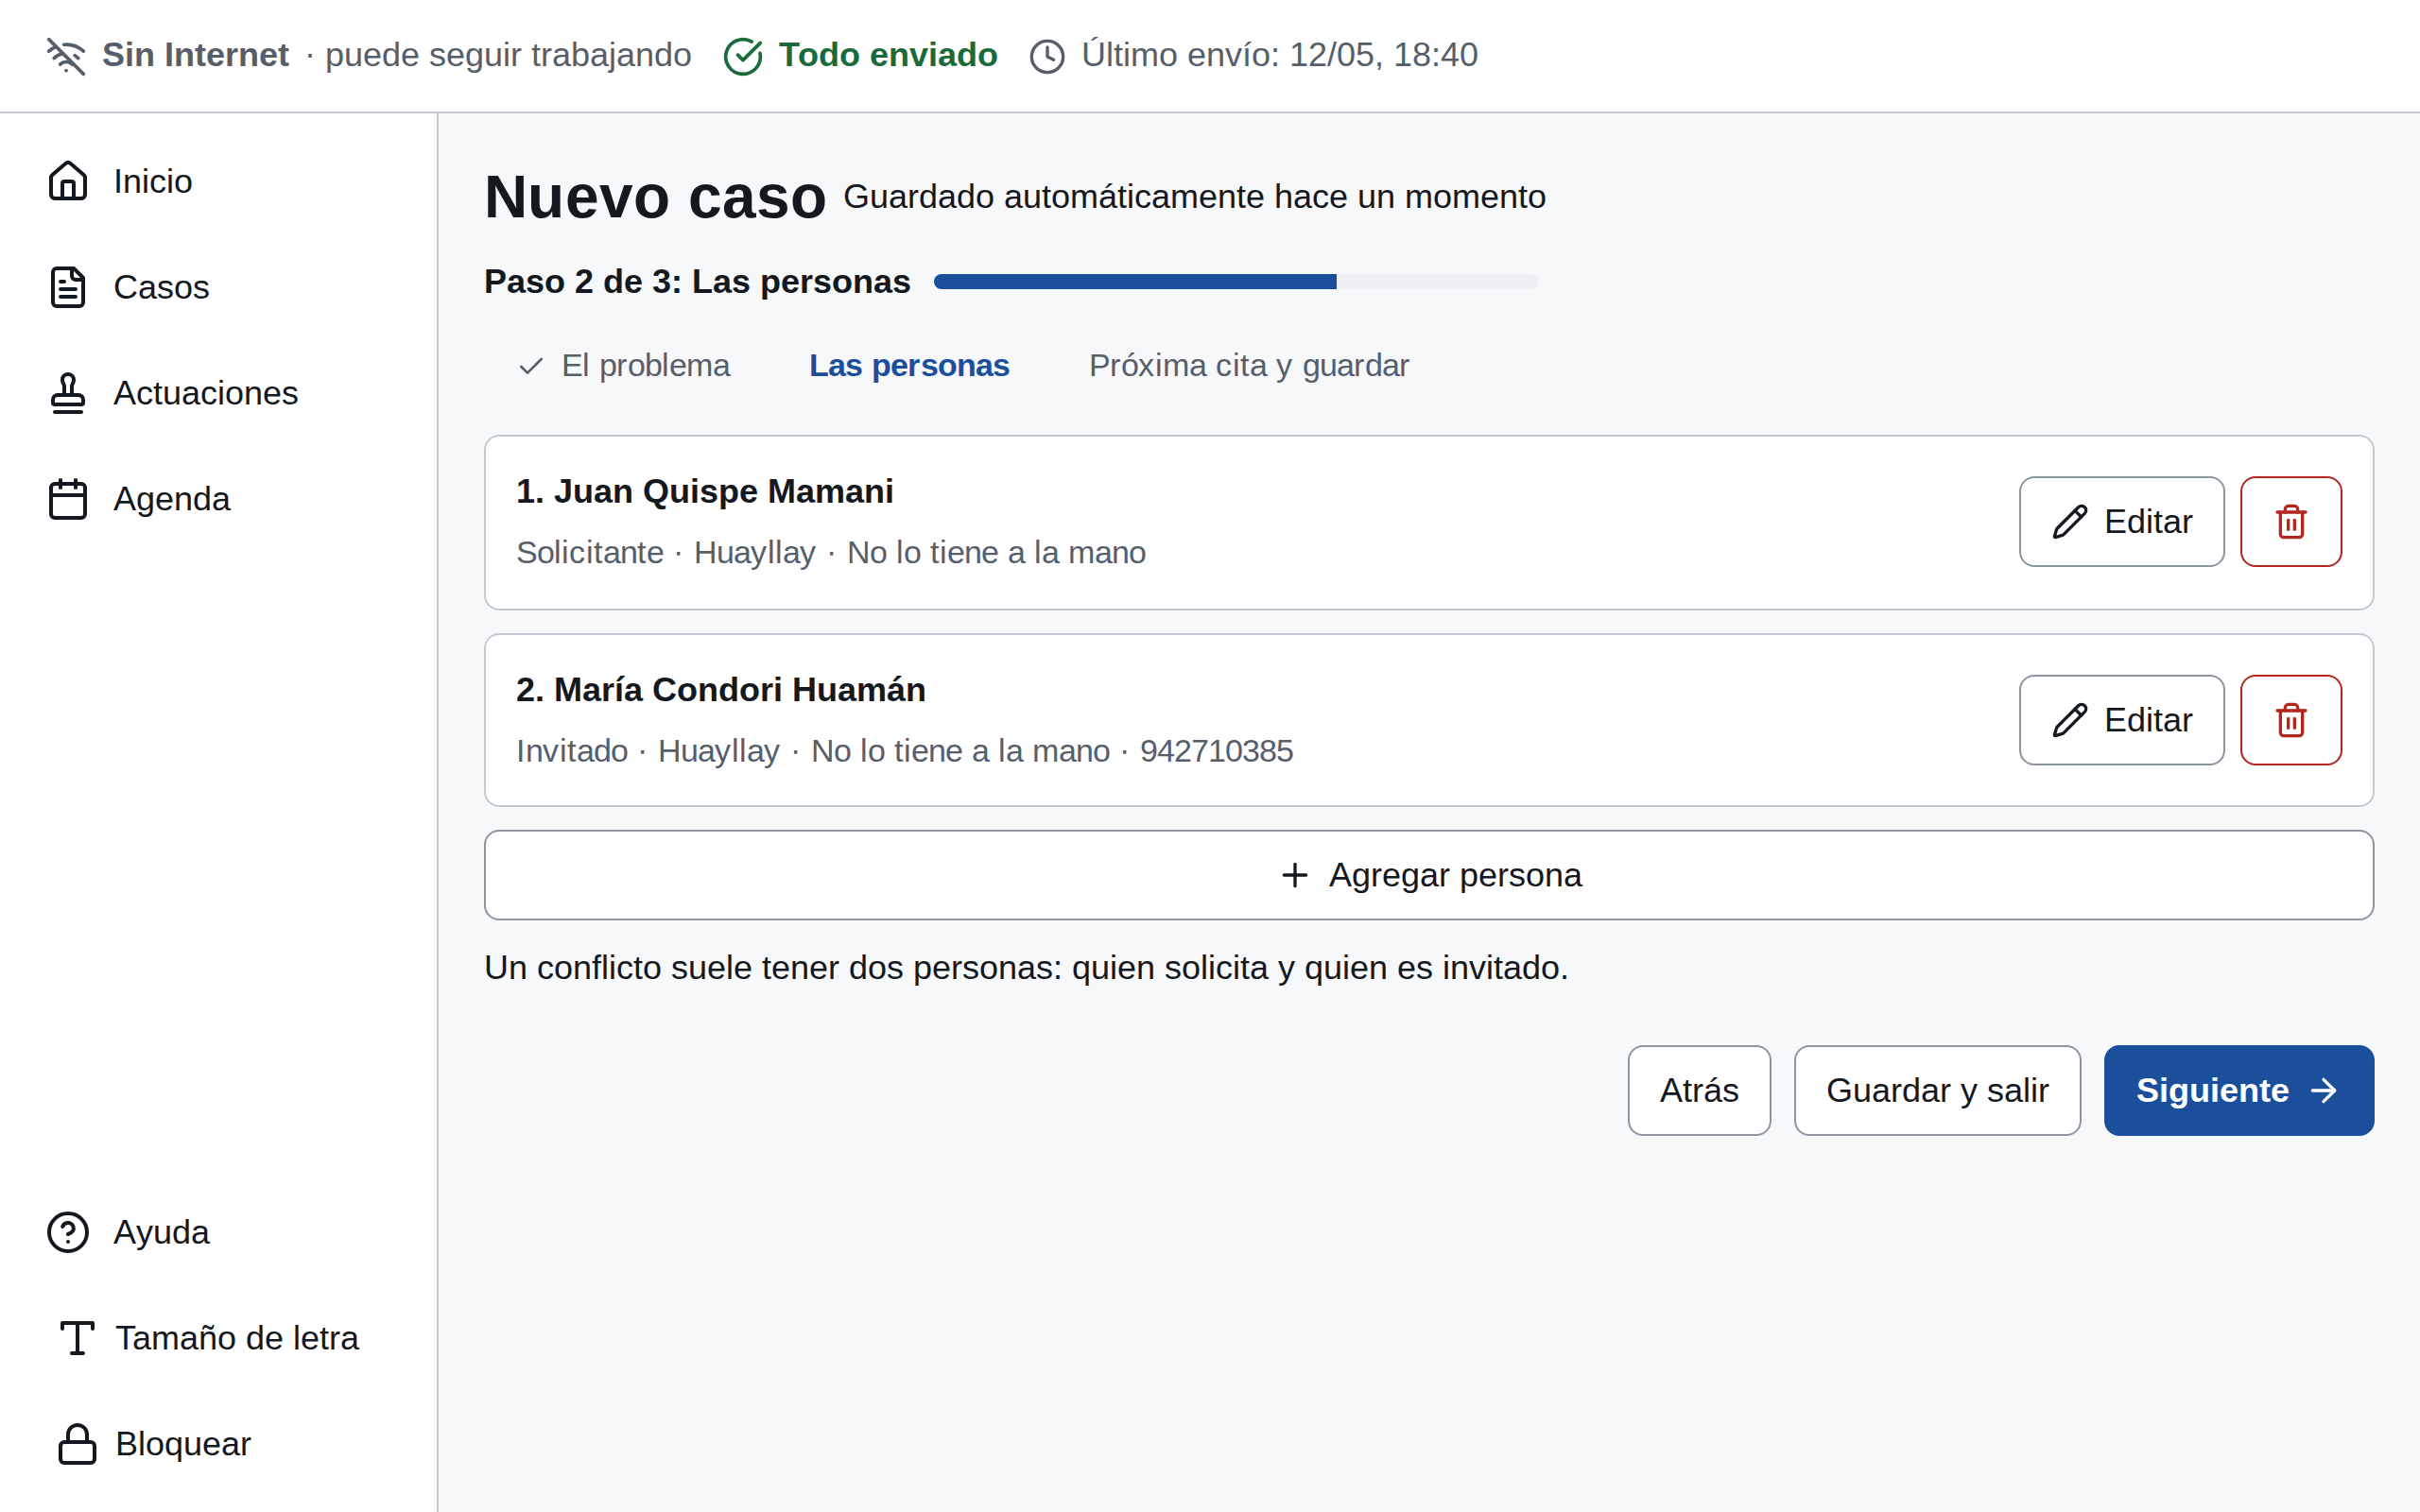
\includegraphics[width=0.82\linewidth]{capturas/F1-08_personas.png}
\caption{P-03 · 5. Las dos partes con su rol. Las partes quedan con rol y comunidad visibles}
\end{figure}
\begin{figure}[H]\centering
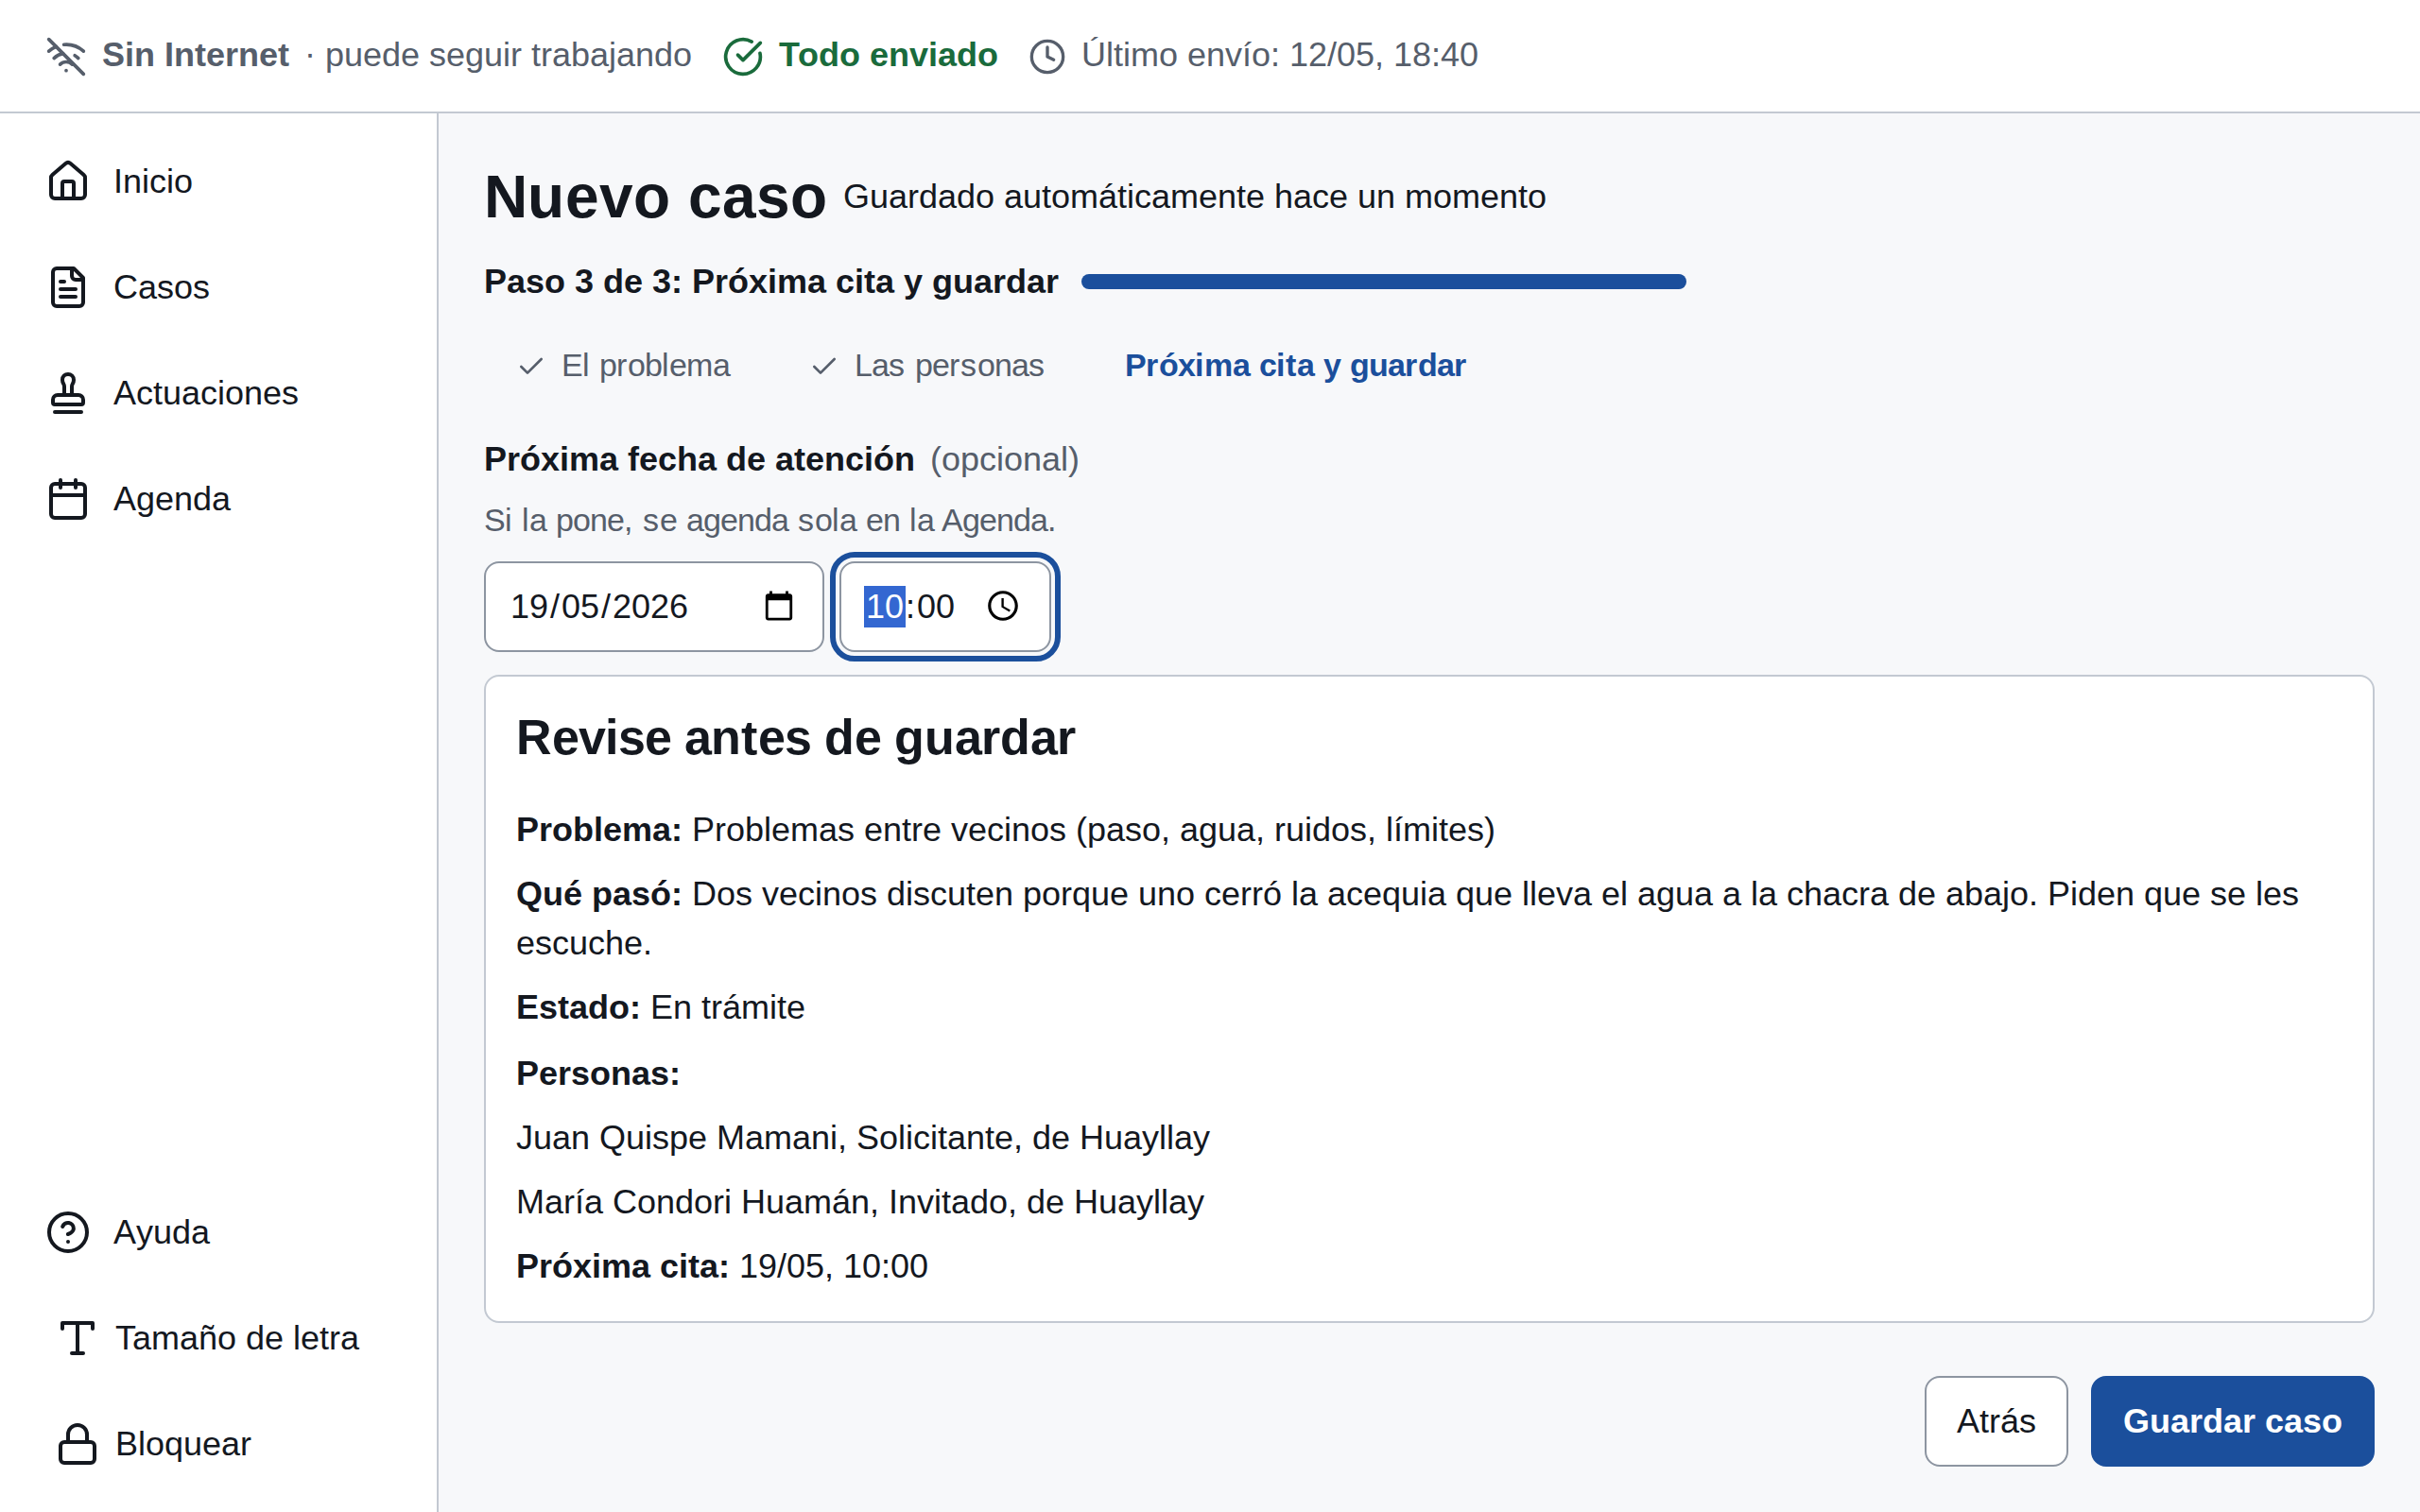
\includegraphics[width=0.82\linewidth]{capturas/F1-09_resumen.png}
\caption{P-03 · 7. Resumen antes de guardar. Resumen legible para leerlo en voz alta a las partes antes de guardar}
\end{figure}
\begin{figure}[H]\centering
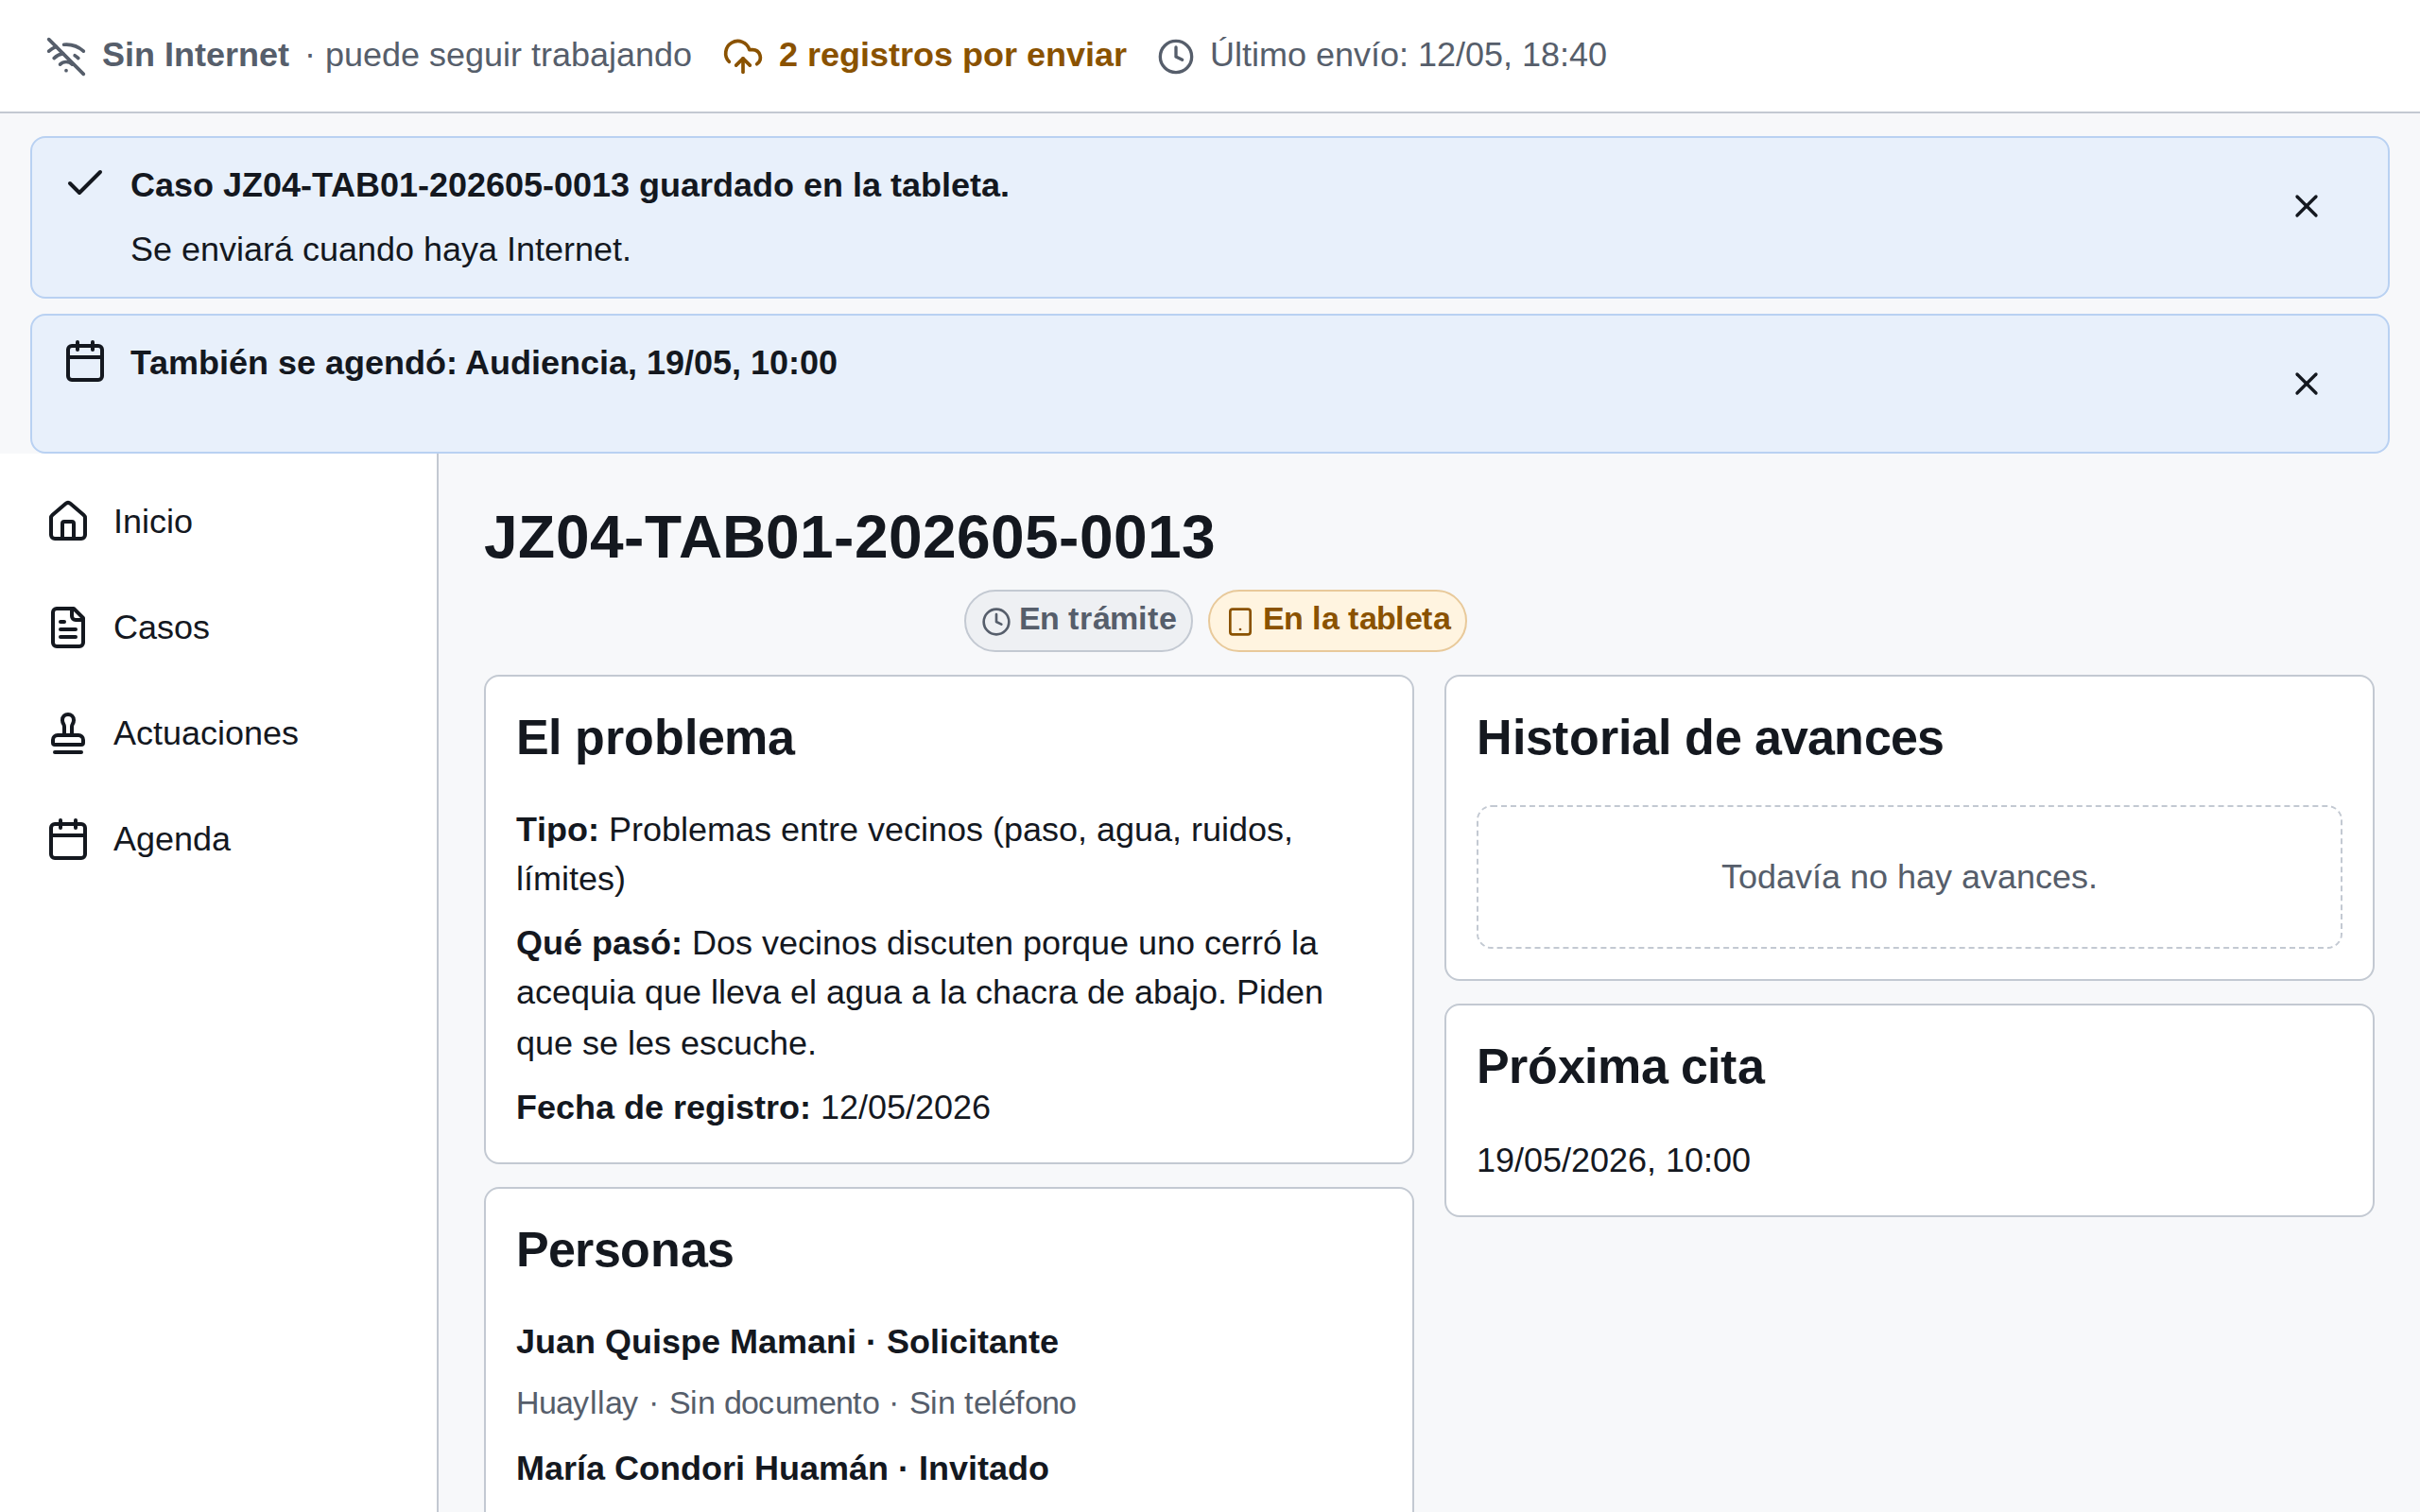
\includegraphics[width=0.82\linewidth]{capturas/F1-10_confirmacion-guardado.png}
\caption{P-04 · 8. Confirmación de guardado. La confirmación dice dónde quedó el caso y que también se agendó la cita}
\end{figure}
\begin{figure}[H]\centering
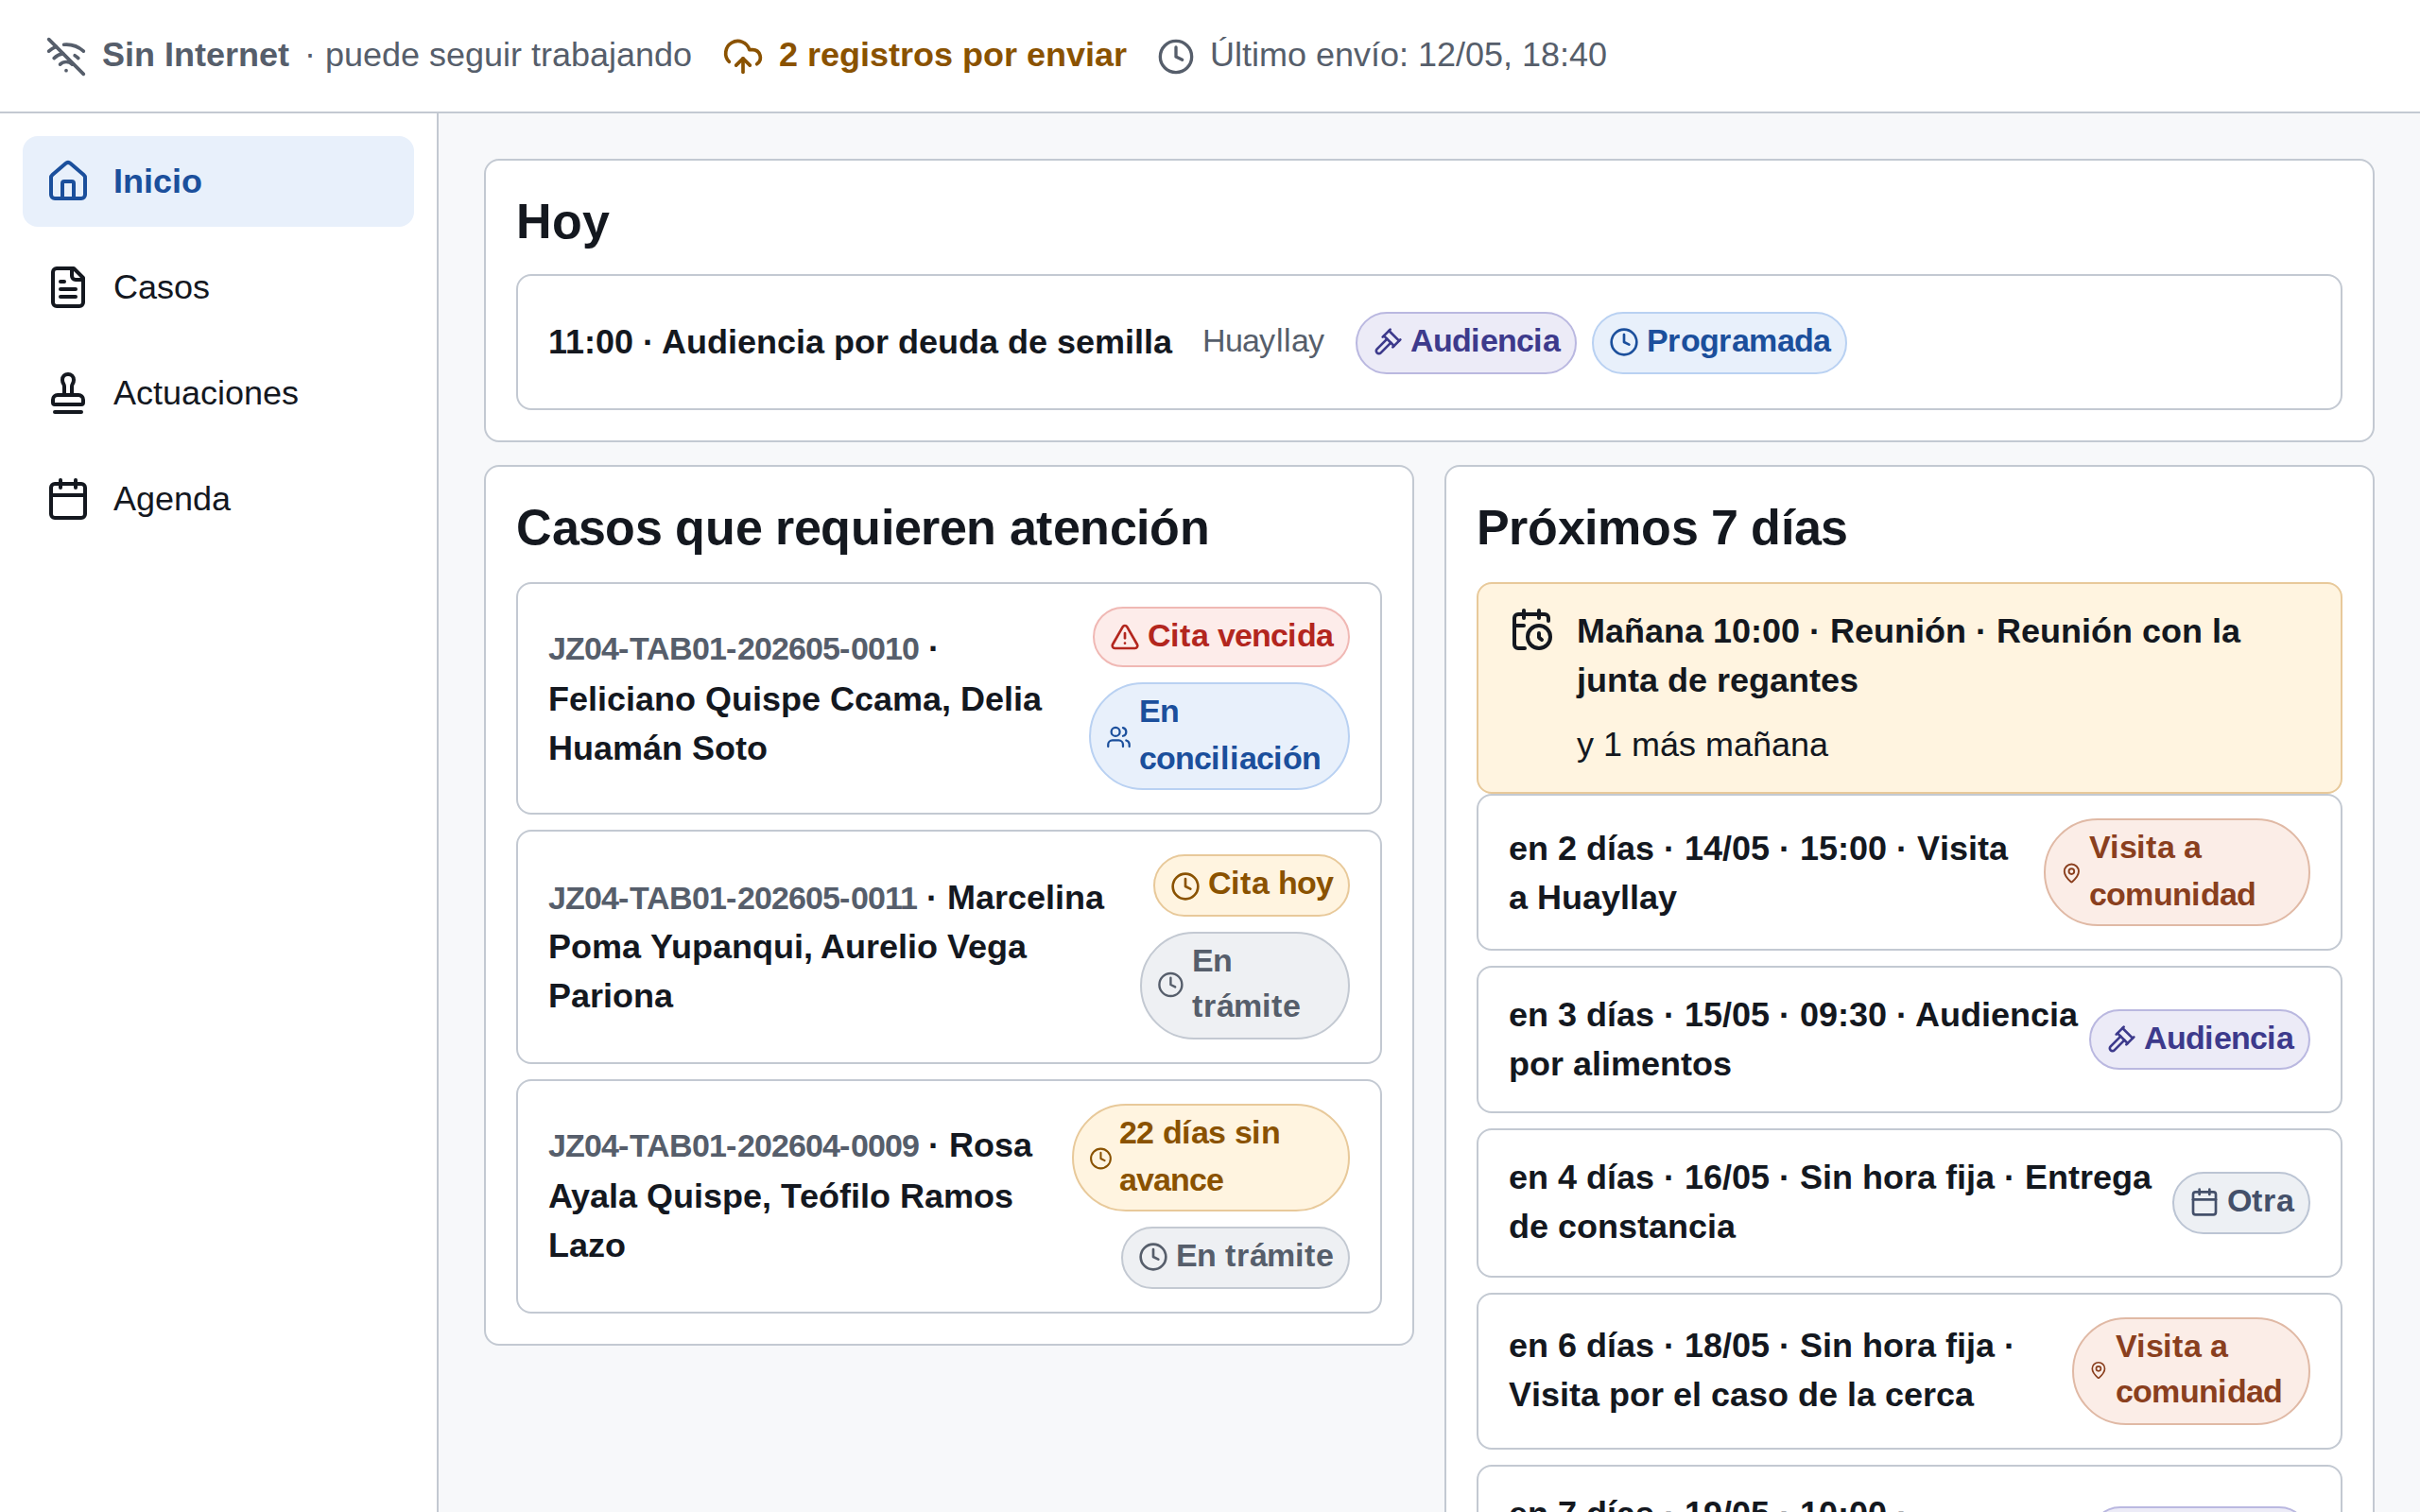
\includegraphics[width=0.82\linewidth]{capturas/F1-11_barra-pendientes.png}
\caption{P-01 · 8. Registros por enviar. El contador de la barra sube solo tras guardar sin Internet: 2 por enviar, el caso y su audiencia}
\end{figure}
\subsection{Flujo 2 · Atender un trámite, con cierre inesperado y recuperación}
\begin{figure}[H]\centering
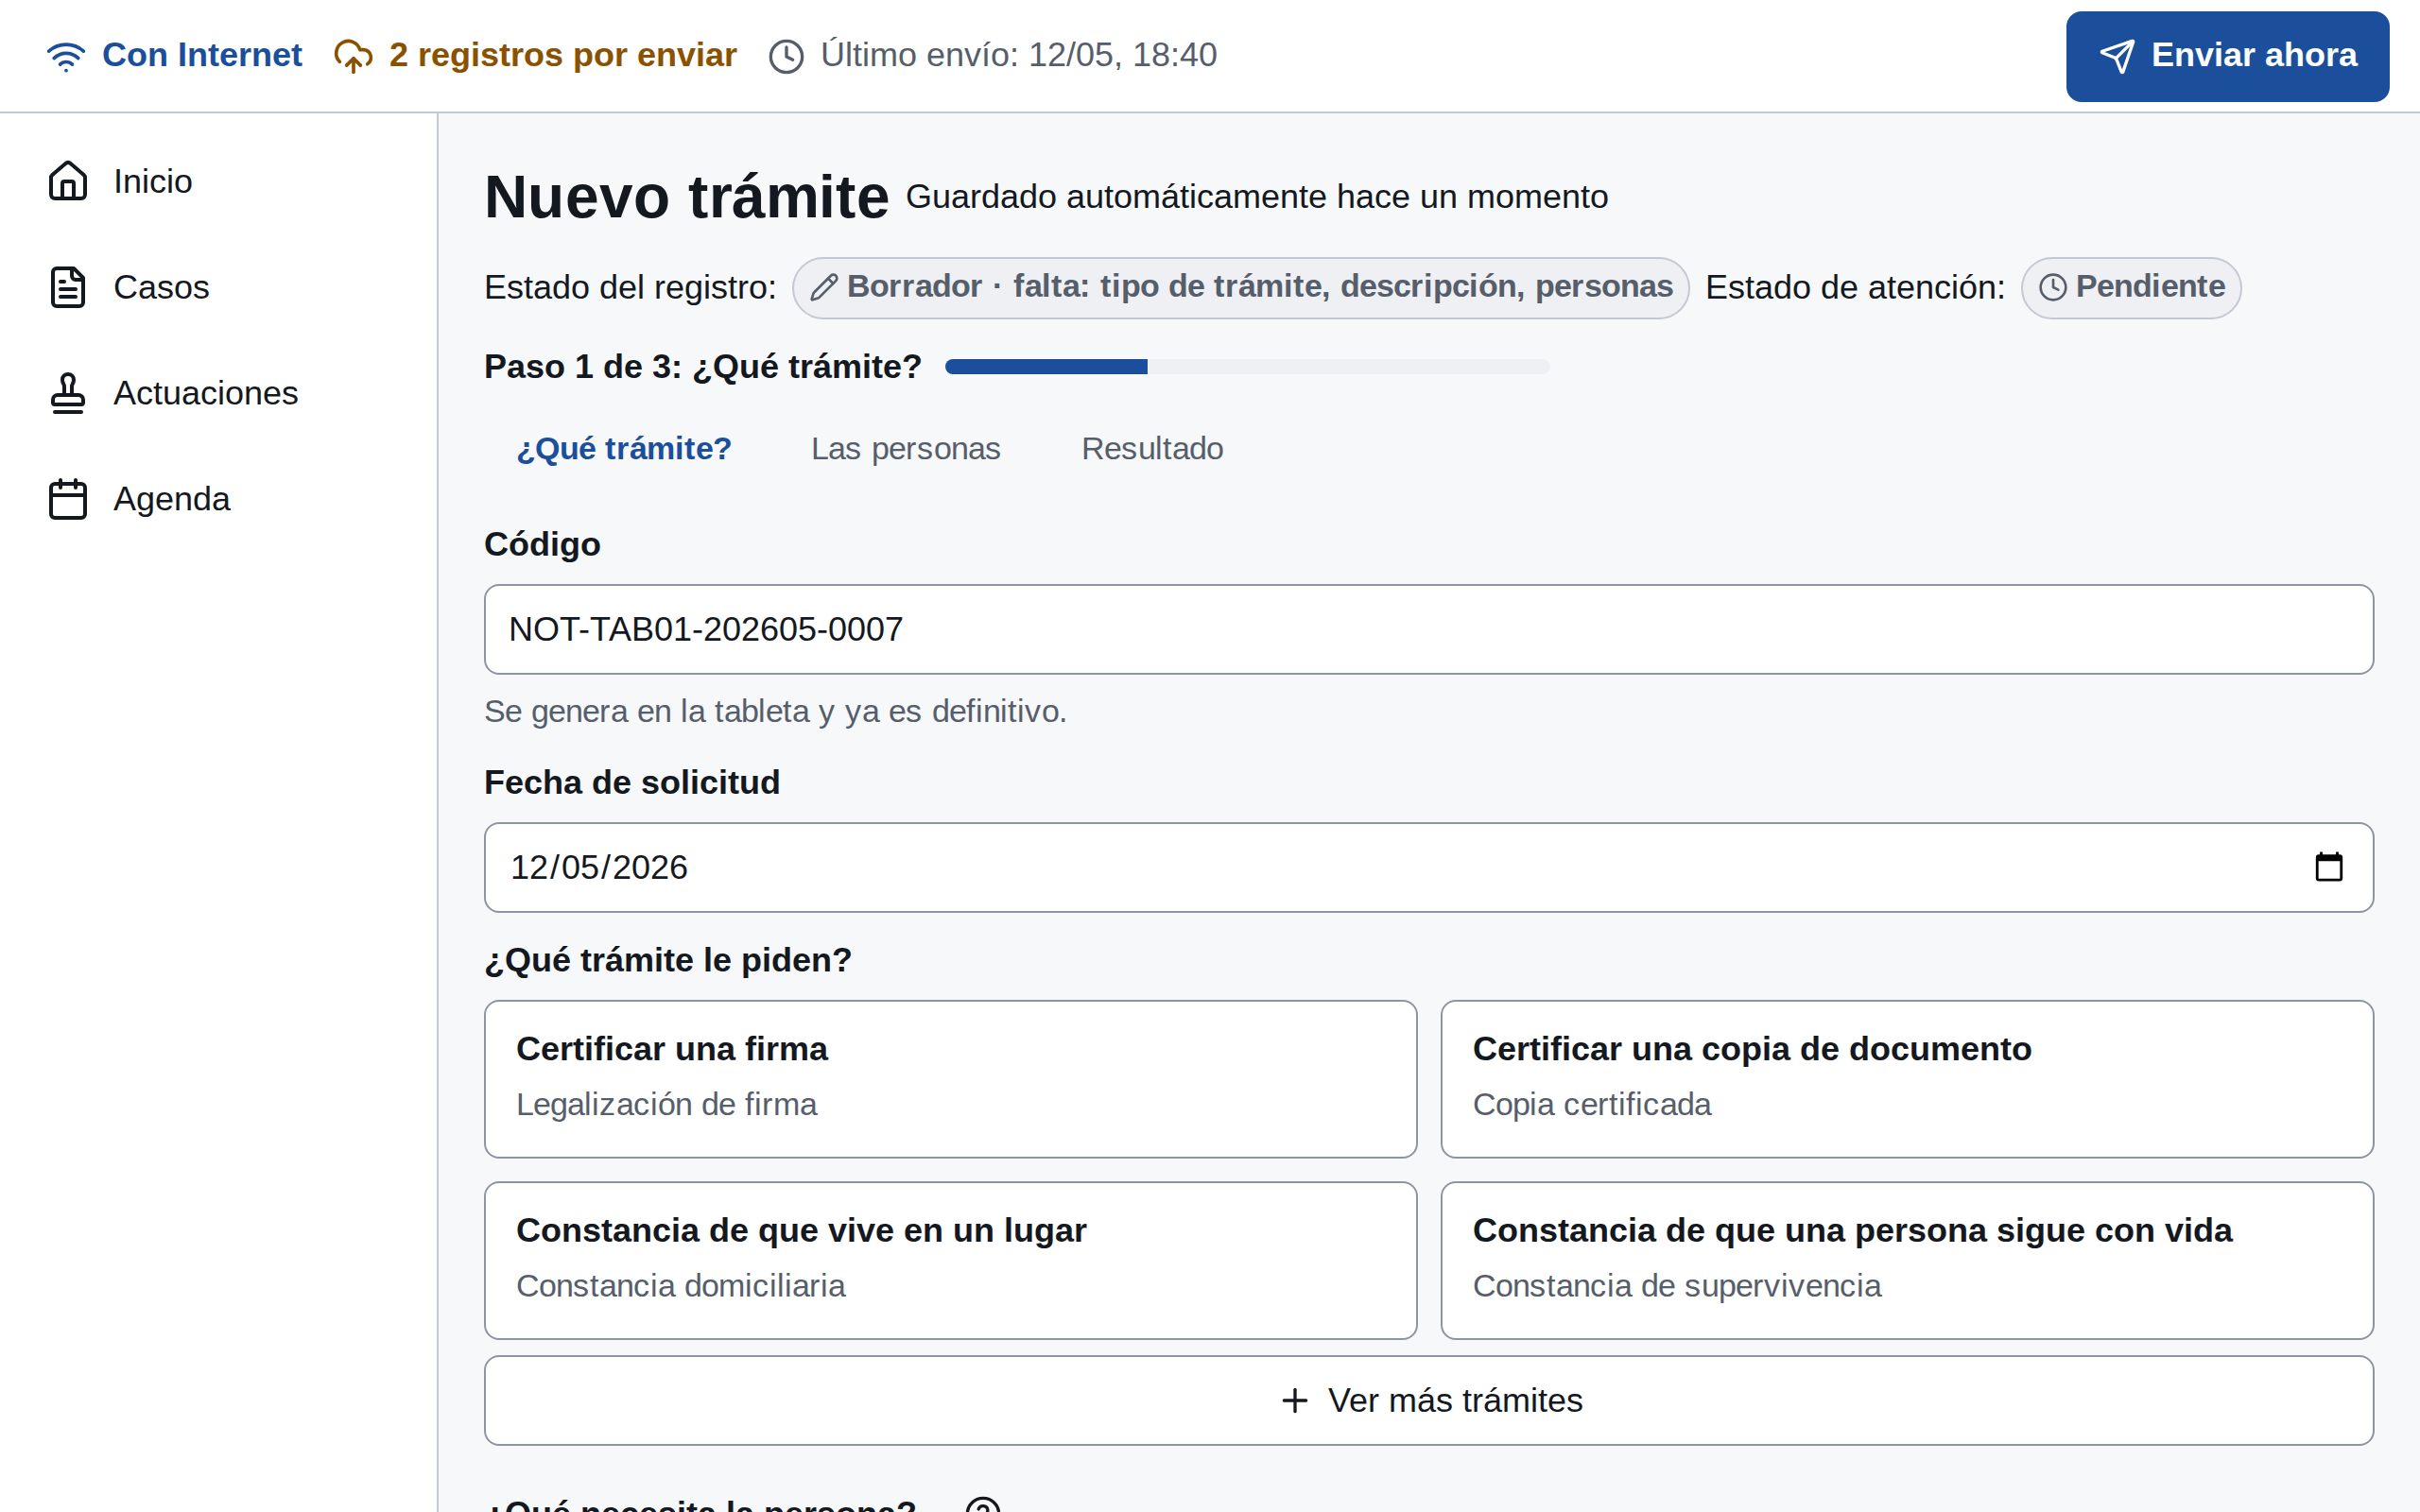
\includegraphics[width=0.82\linewidth]{capturas/F2-01_tramite-paso1.png}
\caption{P-06 · 1. Catálogo de trámites. Cuatro trámites primero, con término legal en gris, y Ver más trámites}
\end{figure}
\begin{figure}[H]\centering
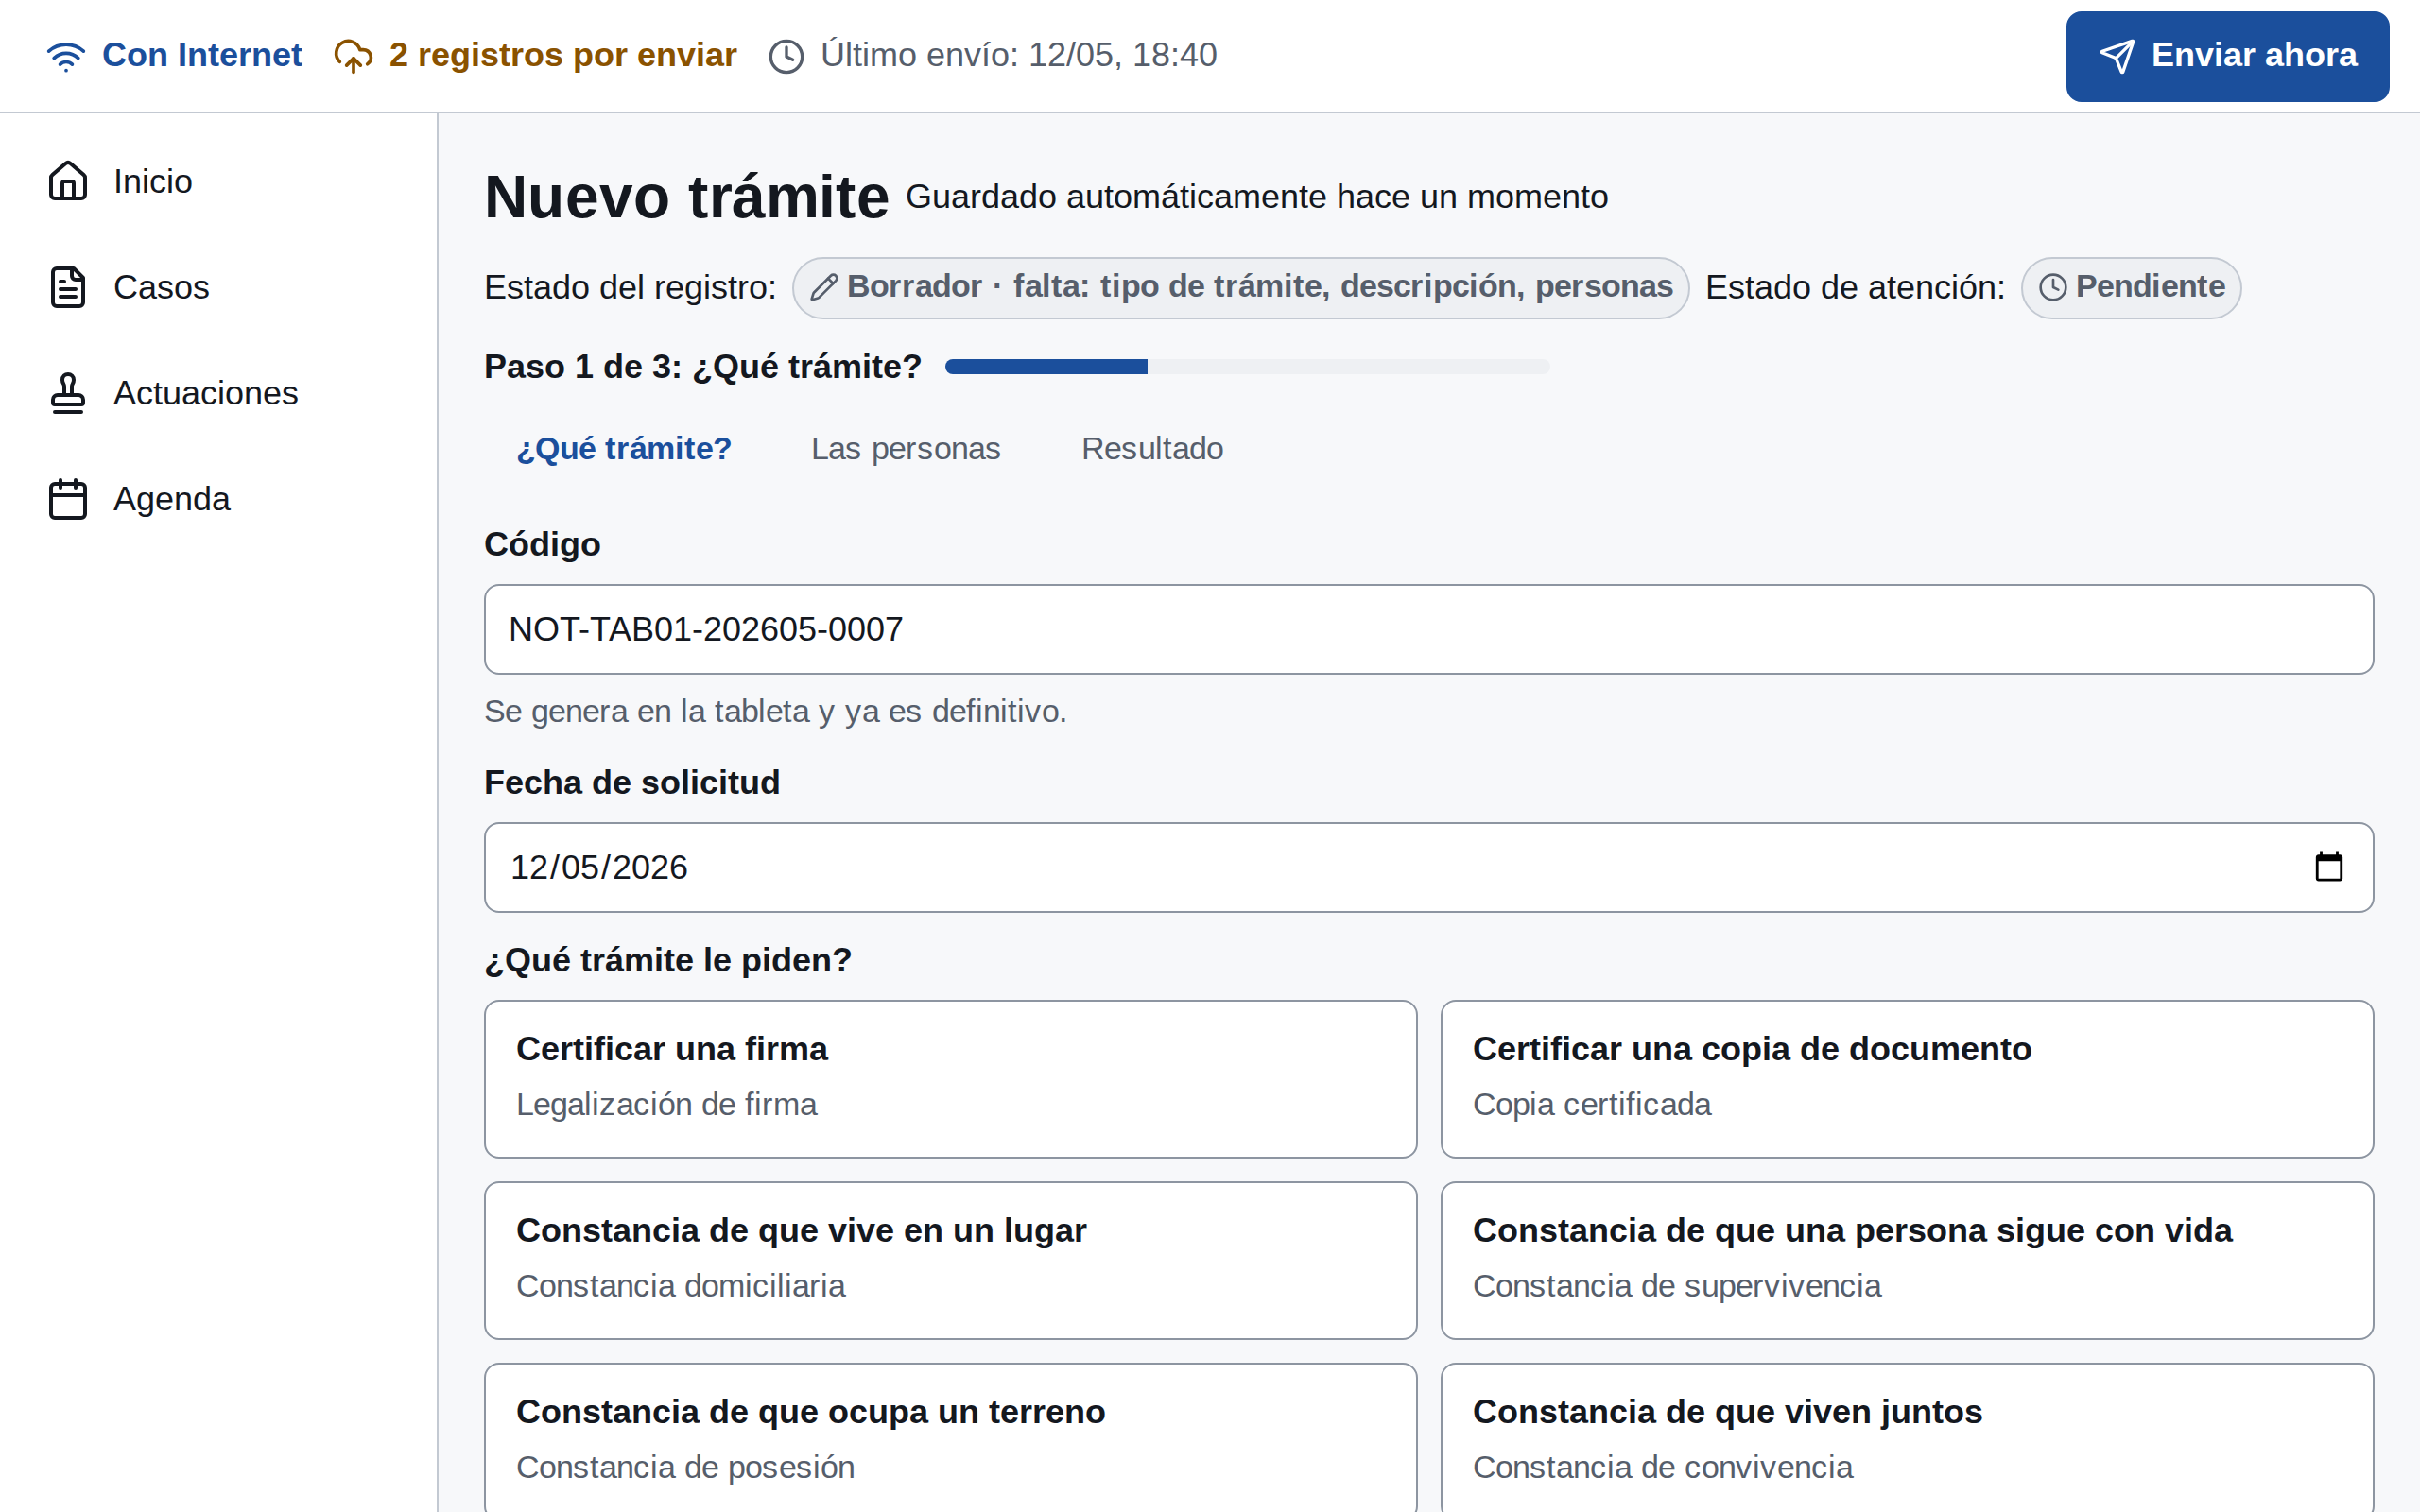
\includegraphics[width=0.82\linewidth]{capturas/F2-02_ver-mas.png}
\caption{P-06 · 1. Catálogo completo. El resto del catálogo aparece sin salir del paso}
\end{figure}
\begin{figure}[H]\centering
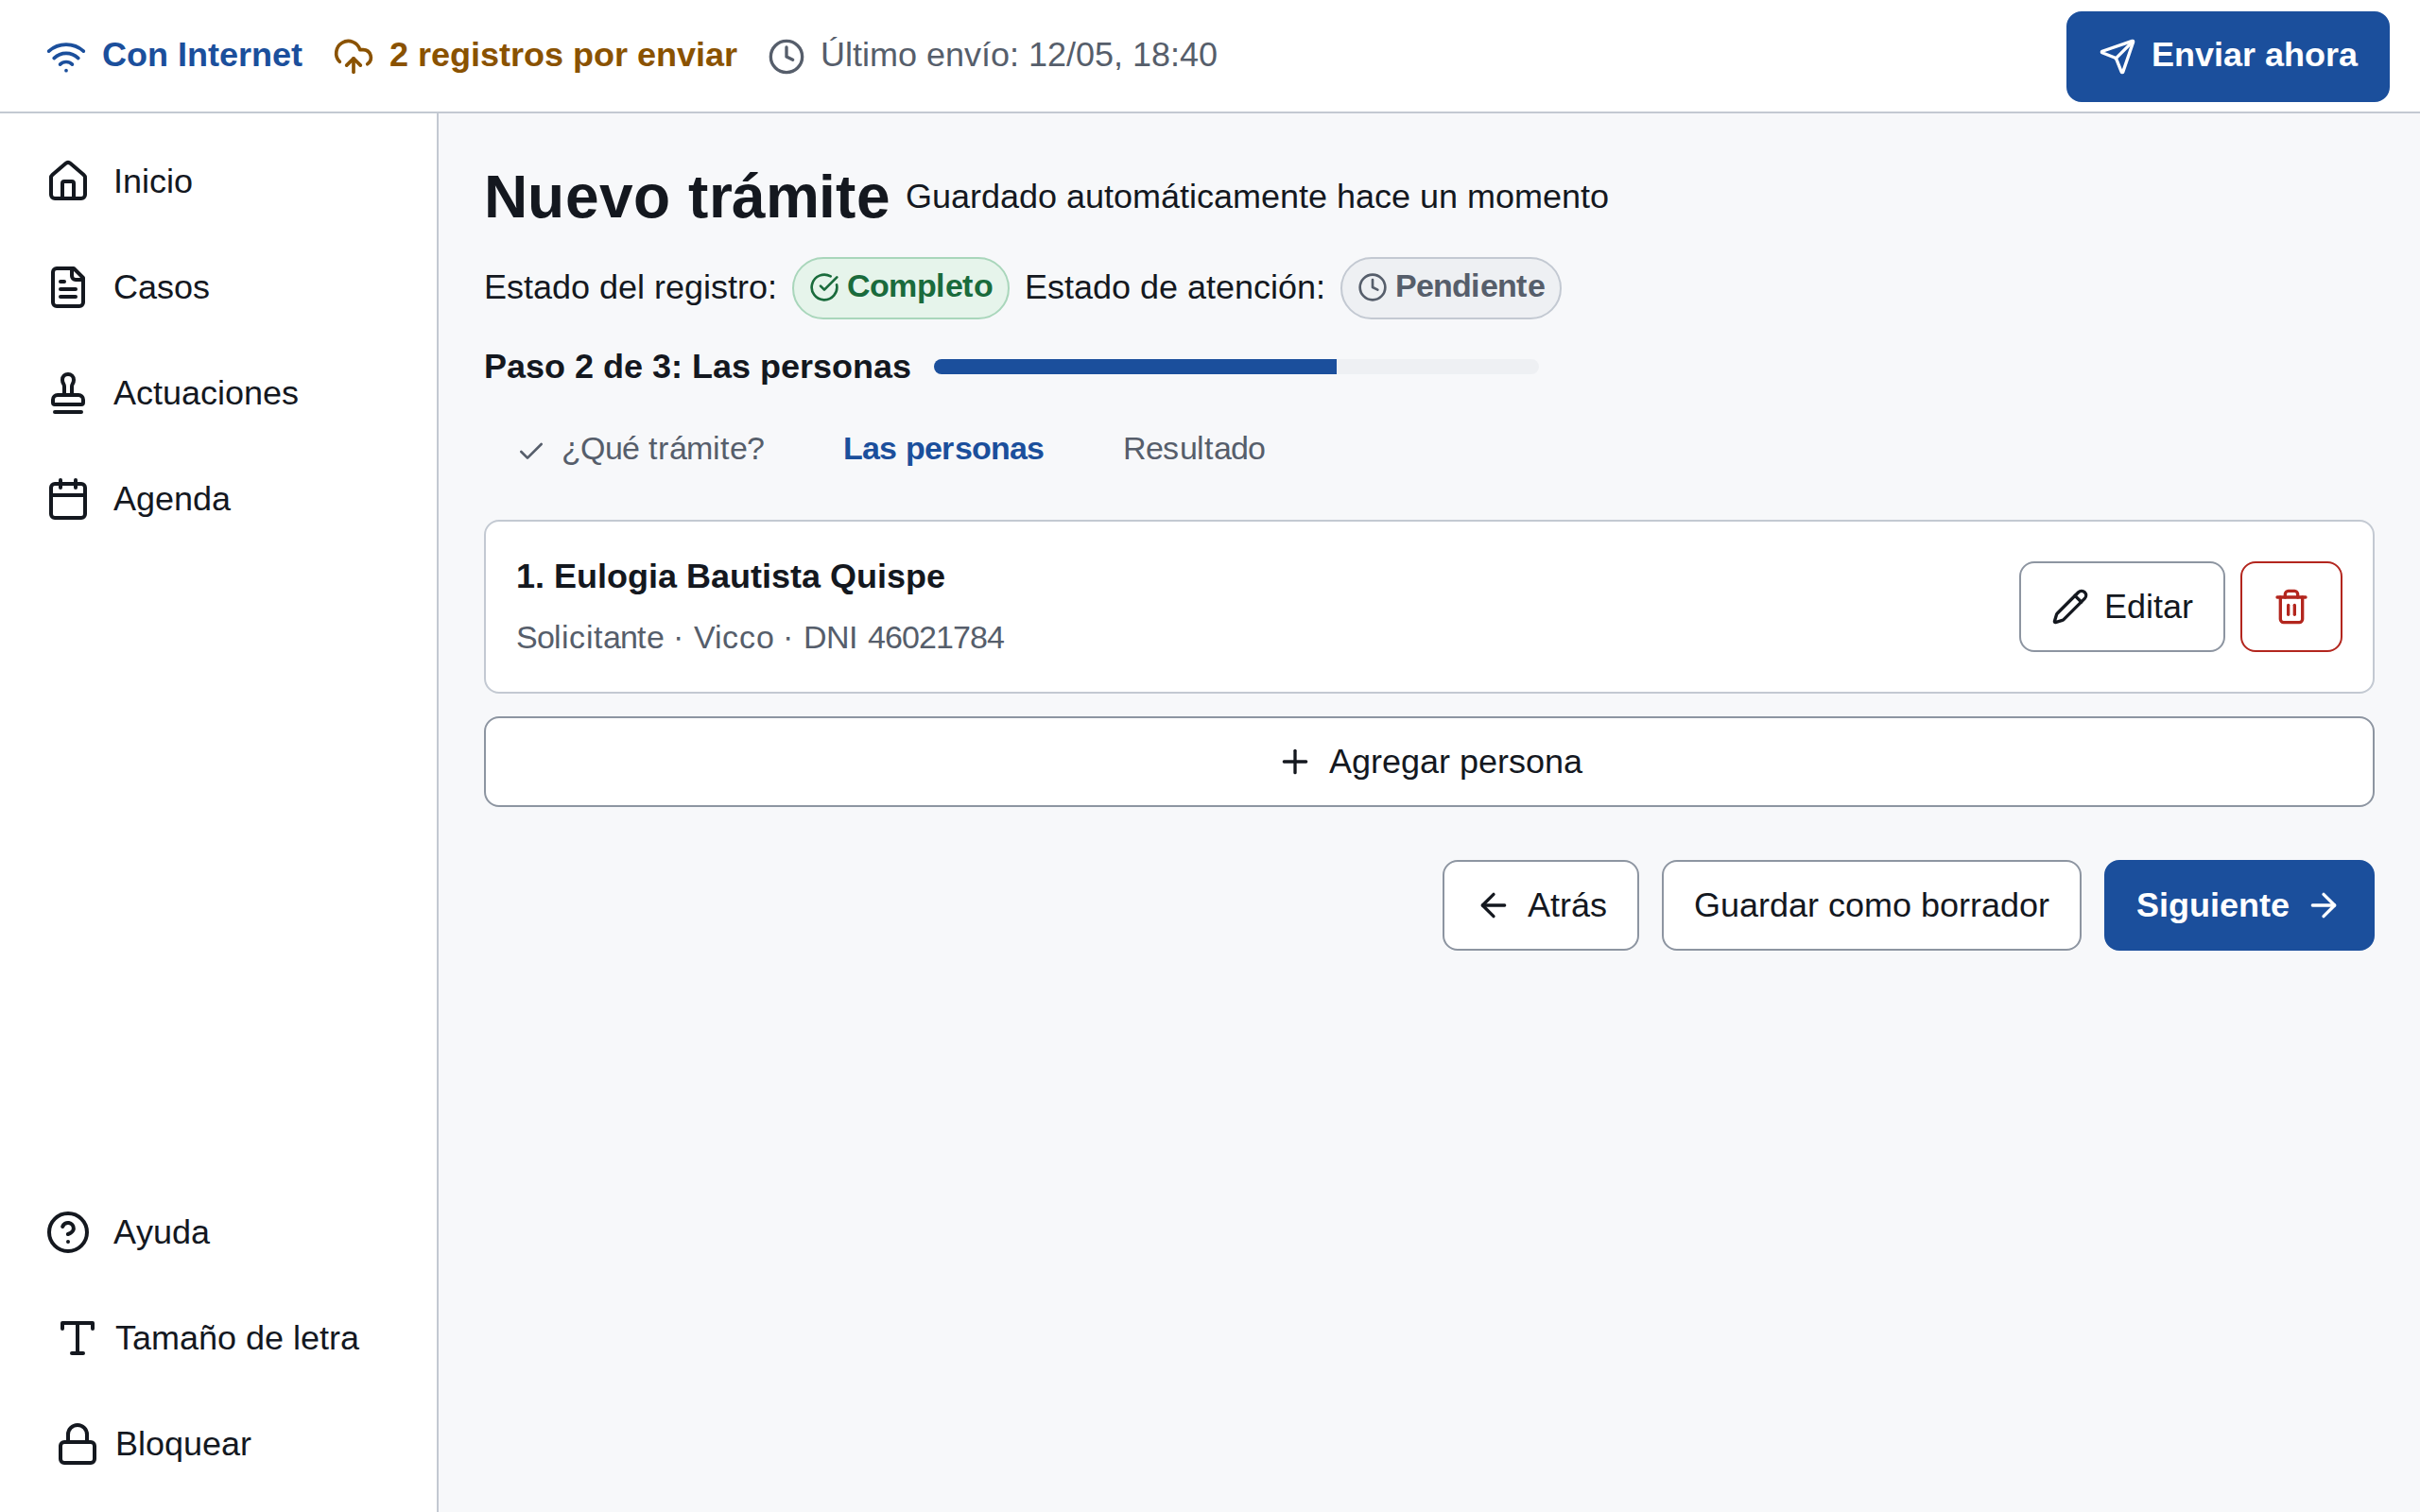
\includegraphics[width=0.82\linewidth]{capturas/F2-03_guardado-automatico.png}
\caption{P-06 · 2. Guardado automático. El texto discreto avisa que lo escrito ya está guardado en la tableta}
\end{figure}
\begin{figure}[H]\centering
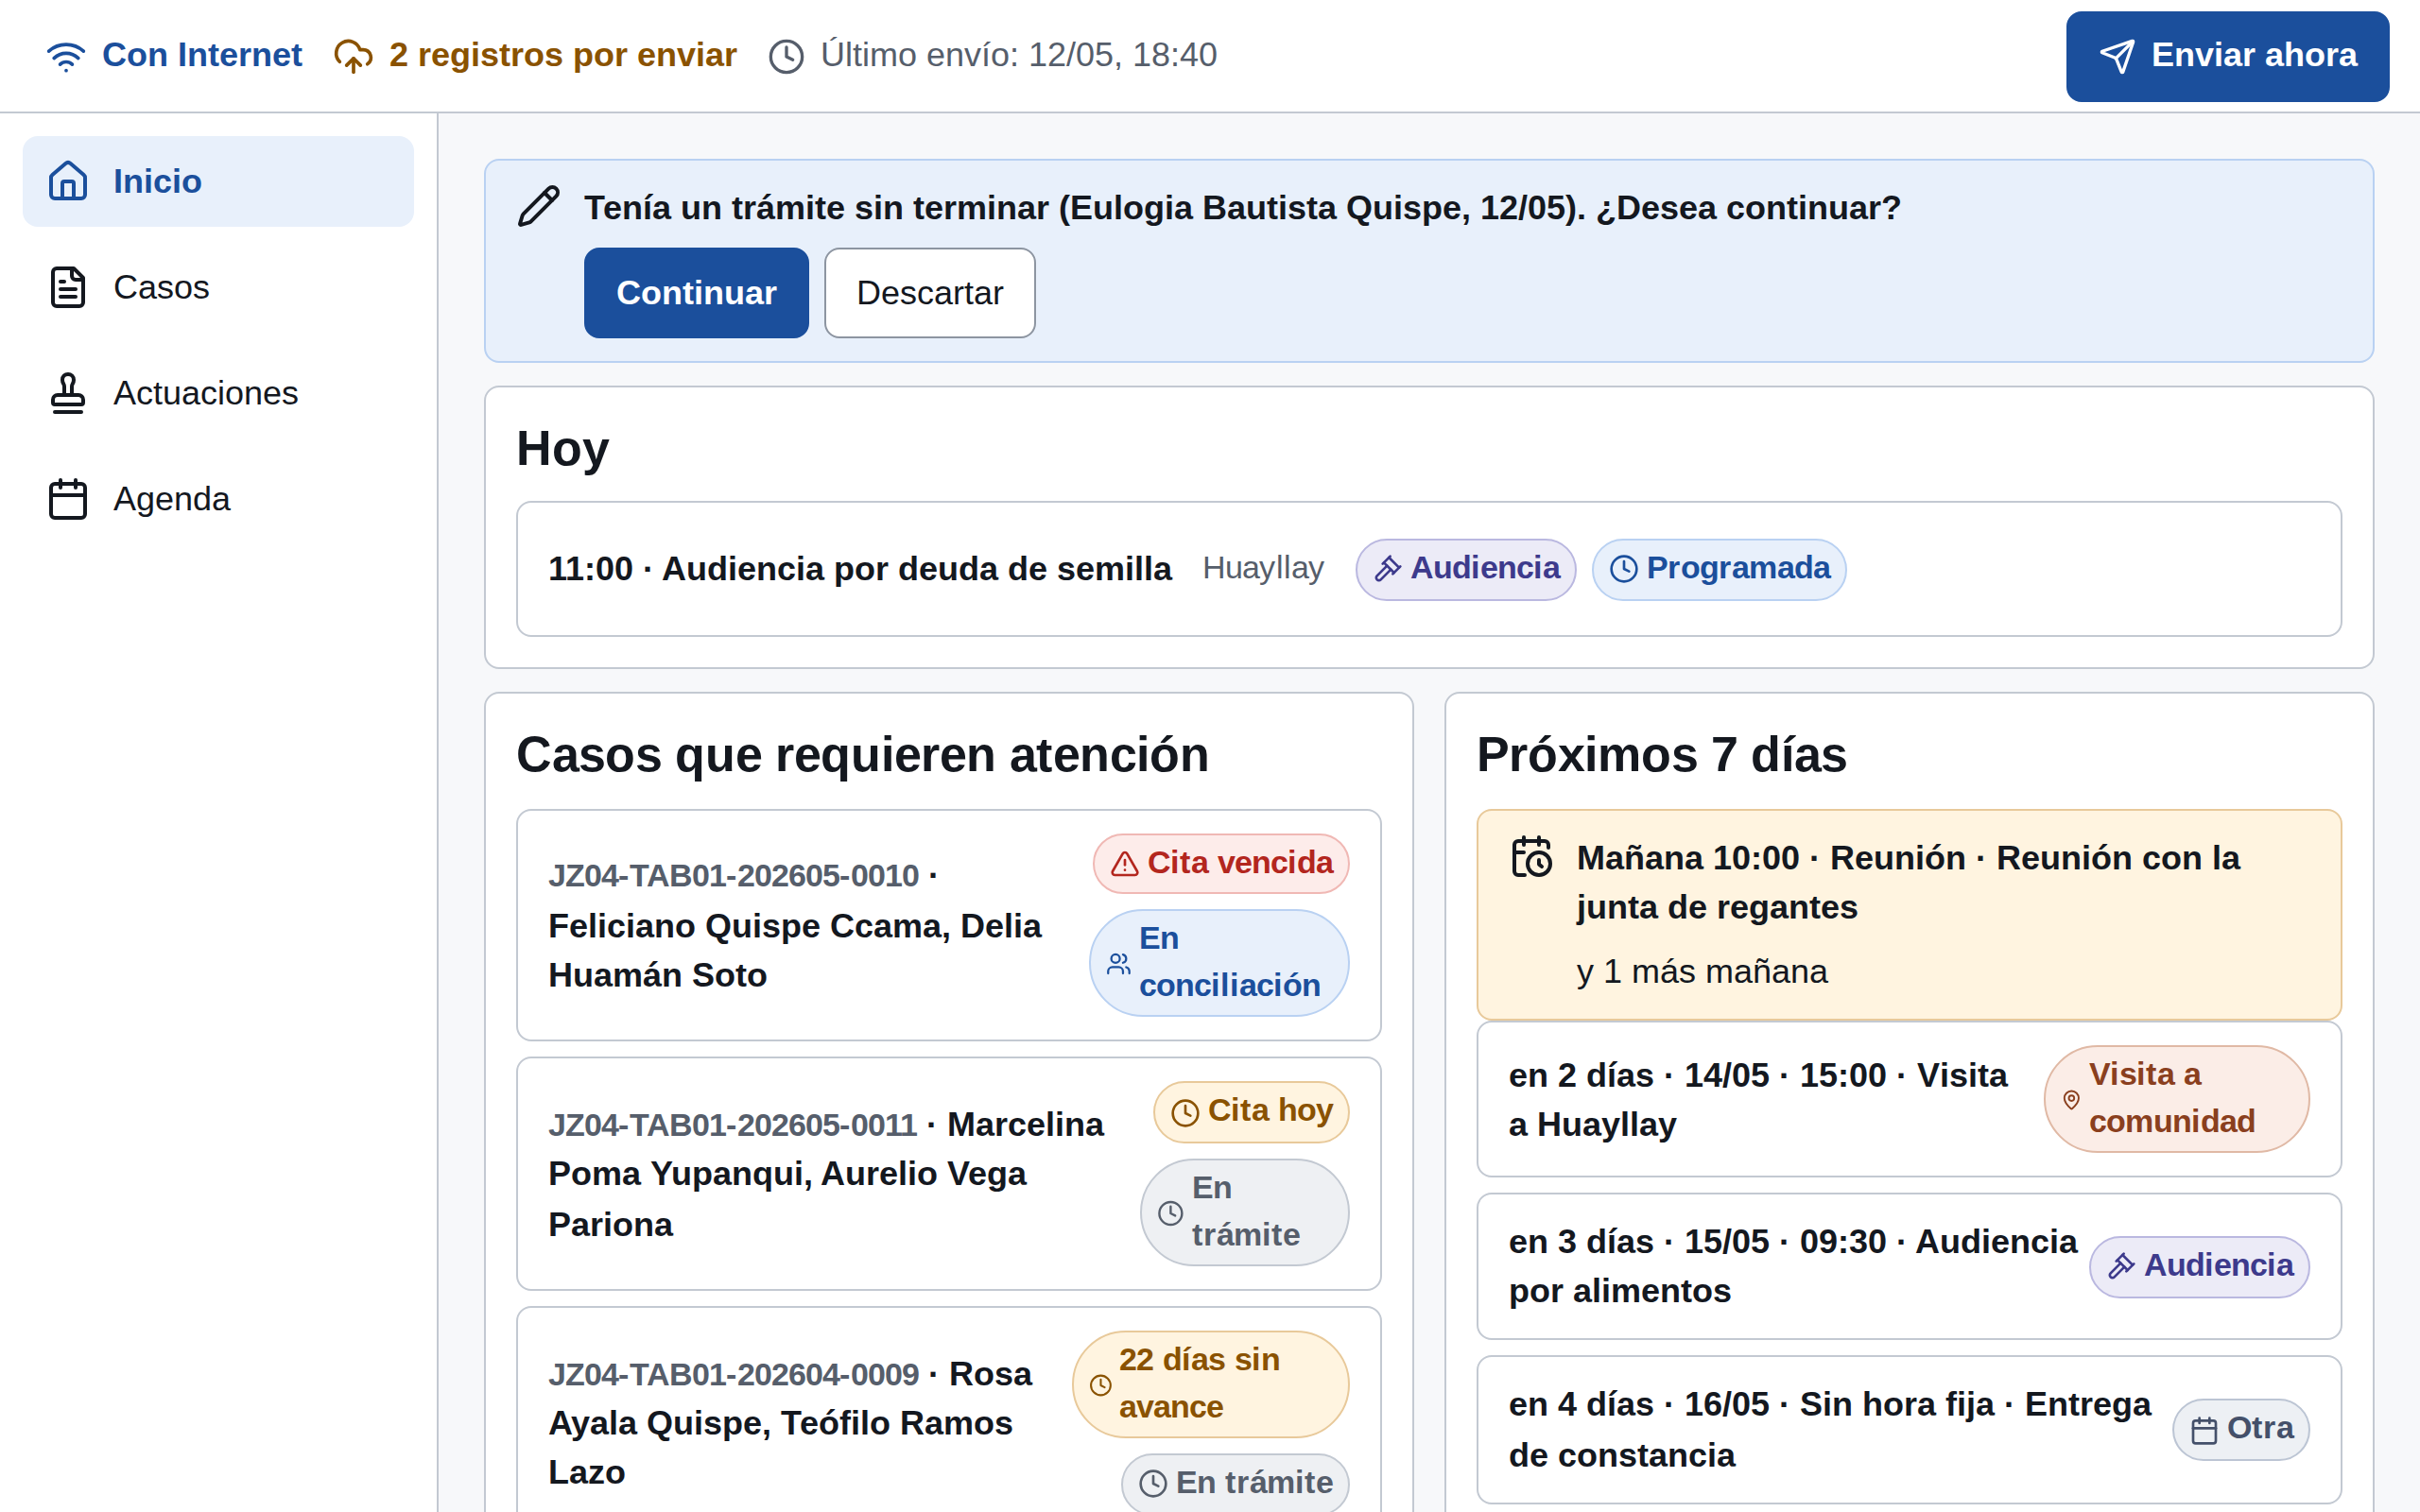
\includegraphics[width=0.82\linewidth]{capturas/F2-04_recuperacion.png}
\caption{P-01 · 3. La aplicación se cerró y se recupera. Al volver, ofrece continuar el trámite sin terminar en vez de perderlo}
\end{figure}
\begin{figure}[H]\centering
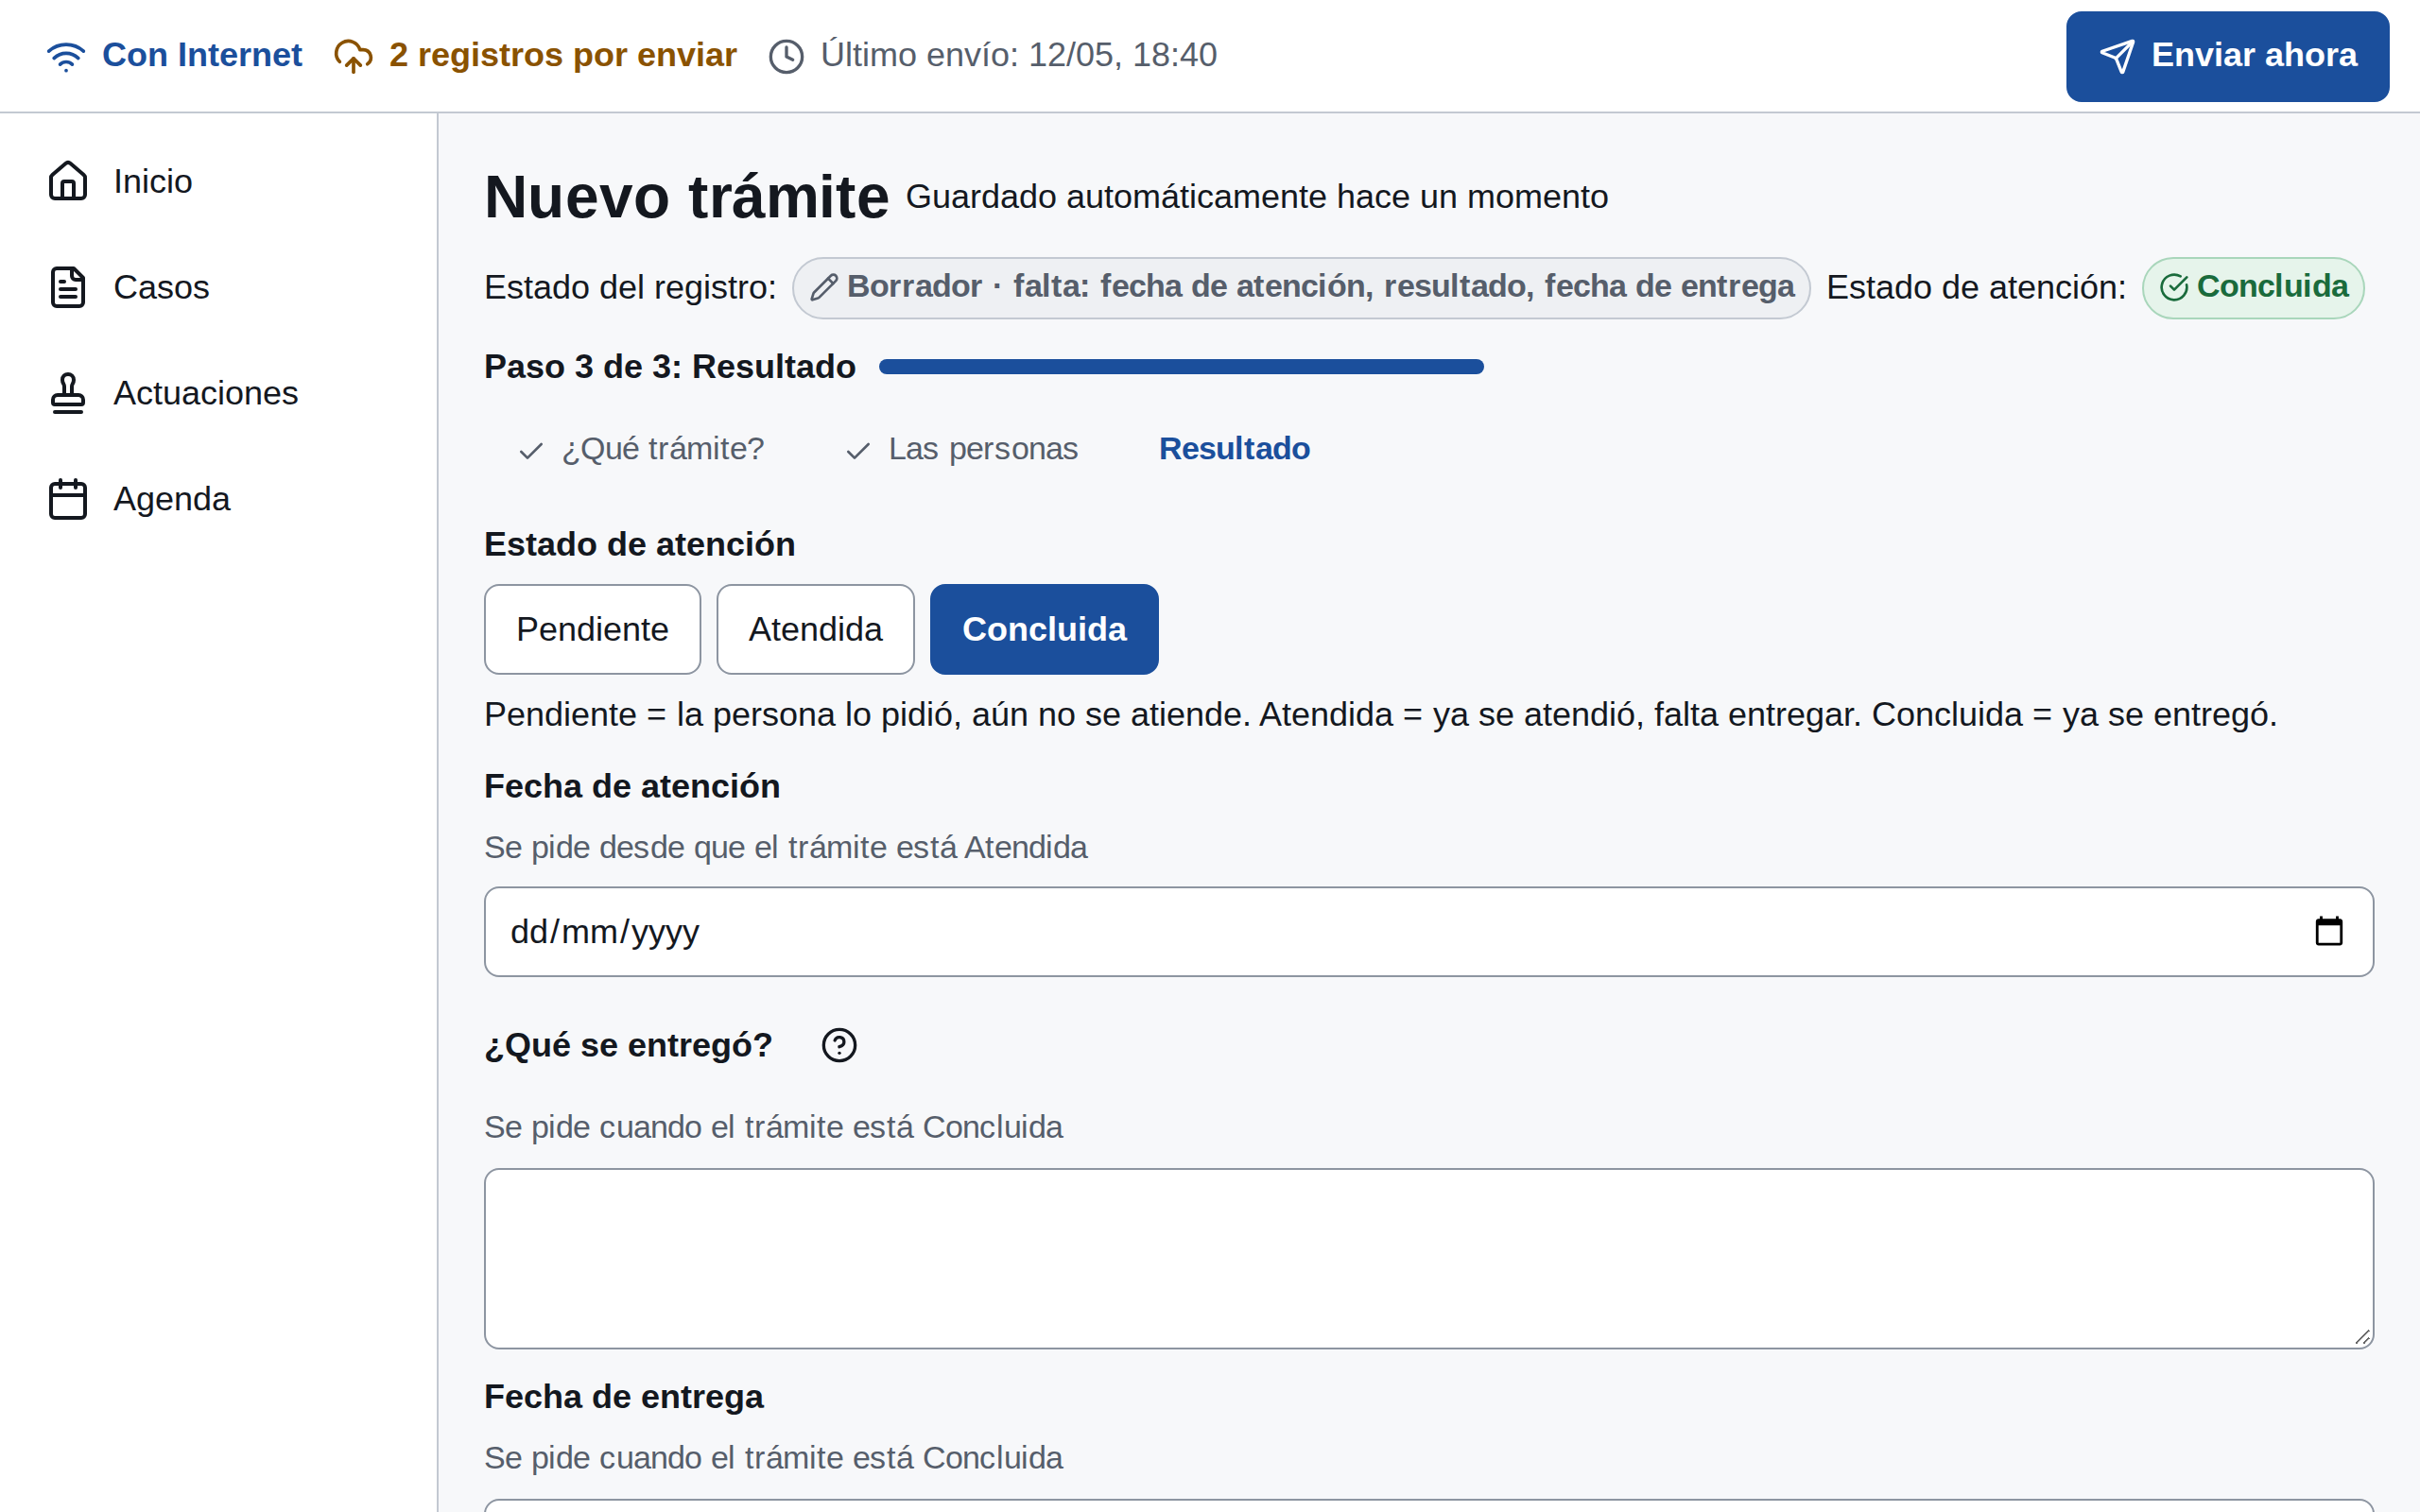
\includegraphics[width=0.82\linewidth]{capturas/F2-05_condicionales.png}
\caption{P-06 · 4. Campos condicionales. Al pasar a Concluida aparecen los campos que se piden, con su línea explicativa}
\end{figure}
\begin{figure}[H]\centering
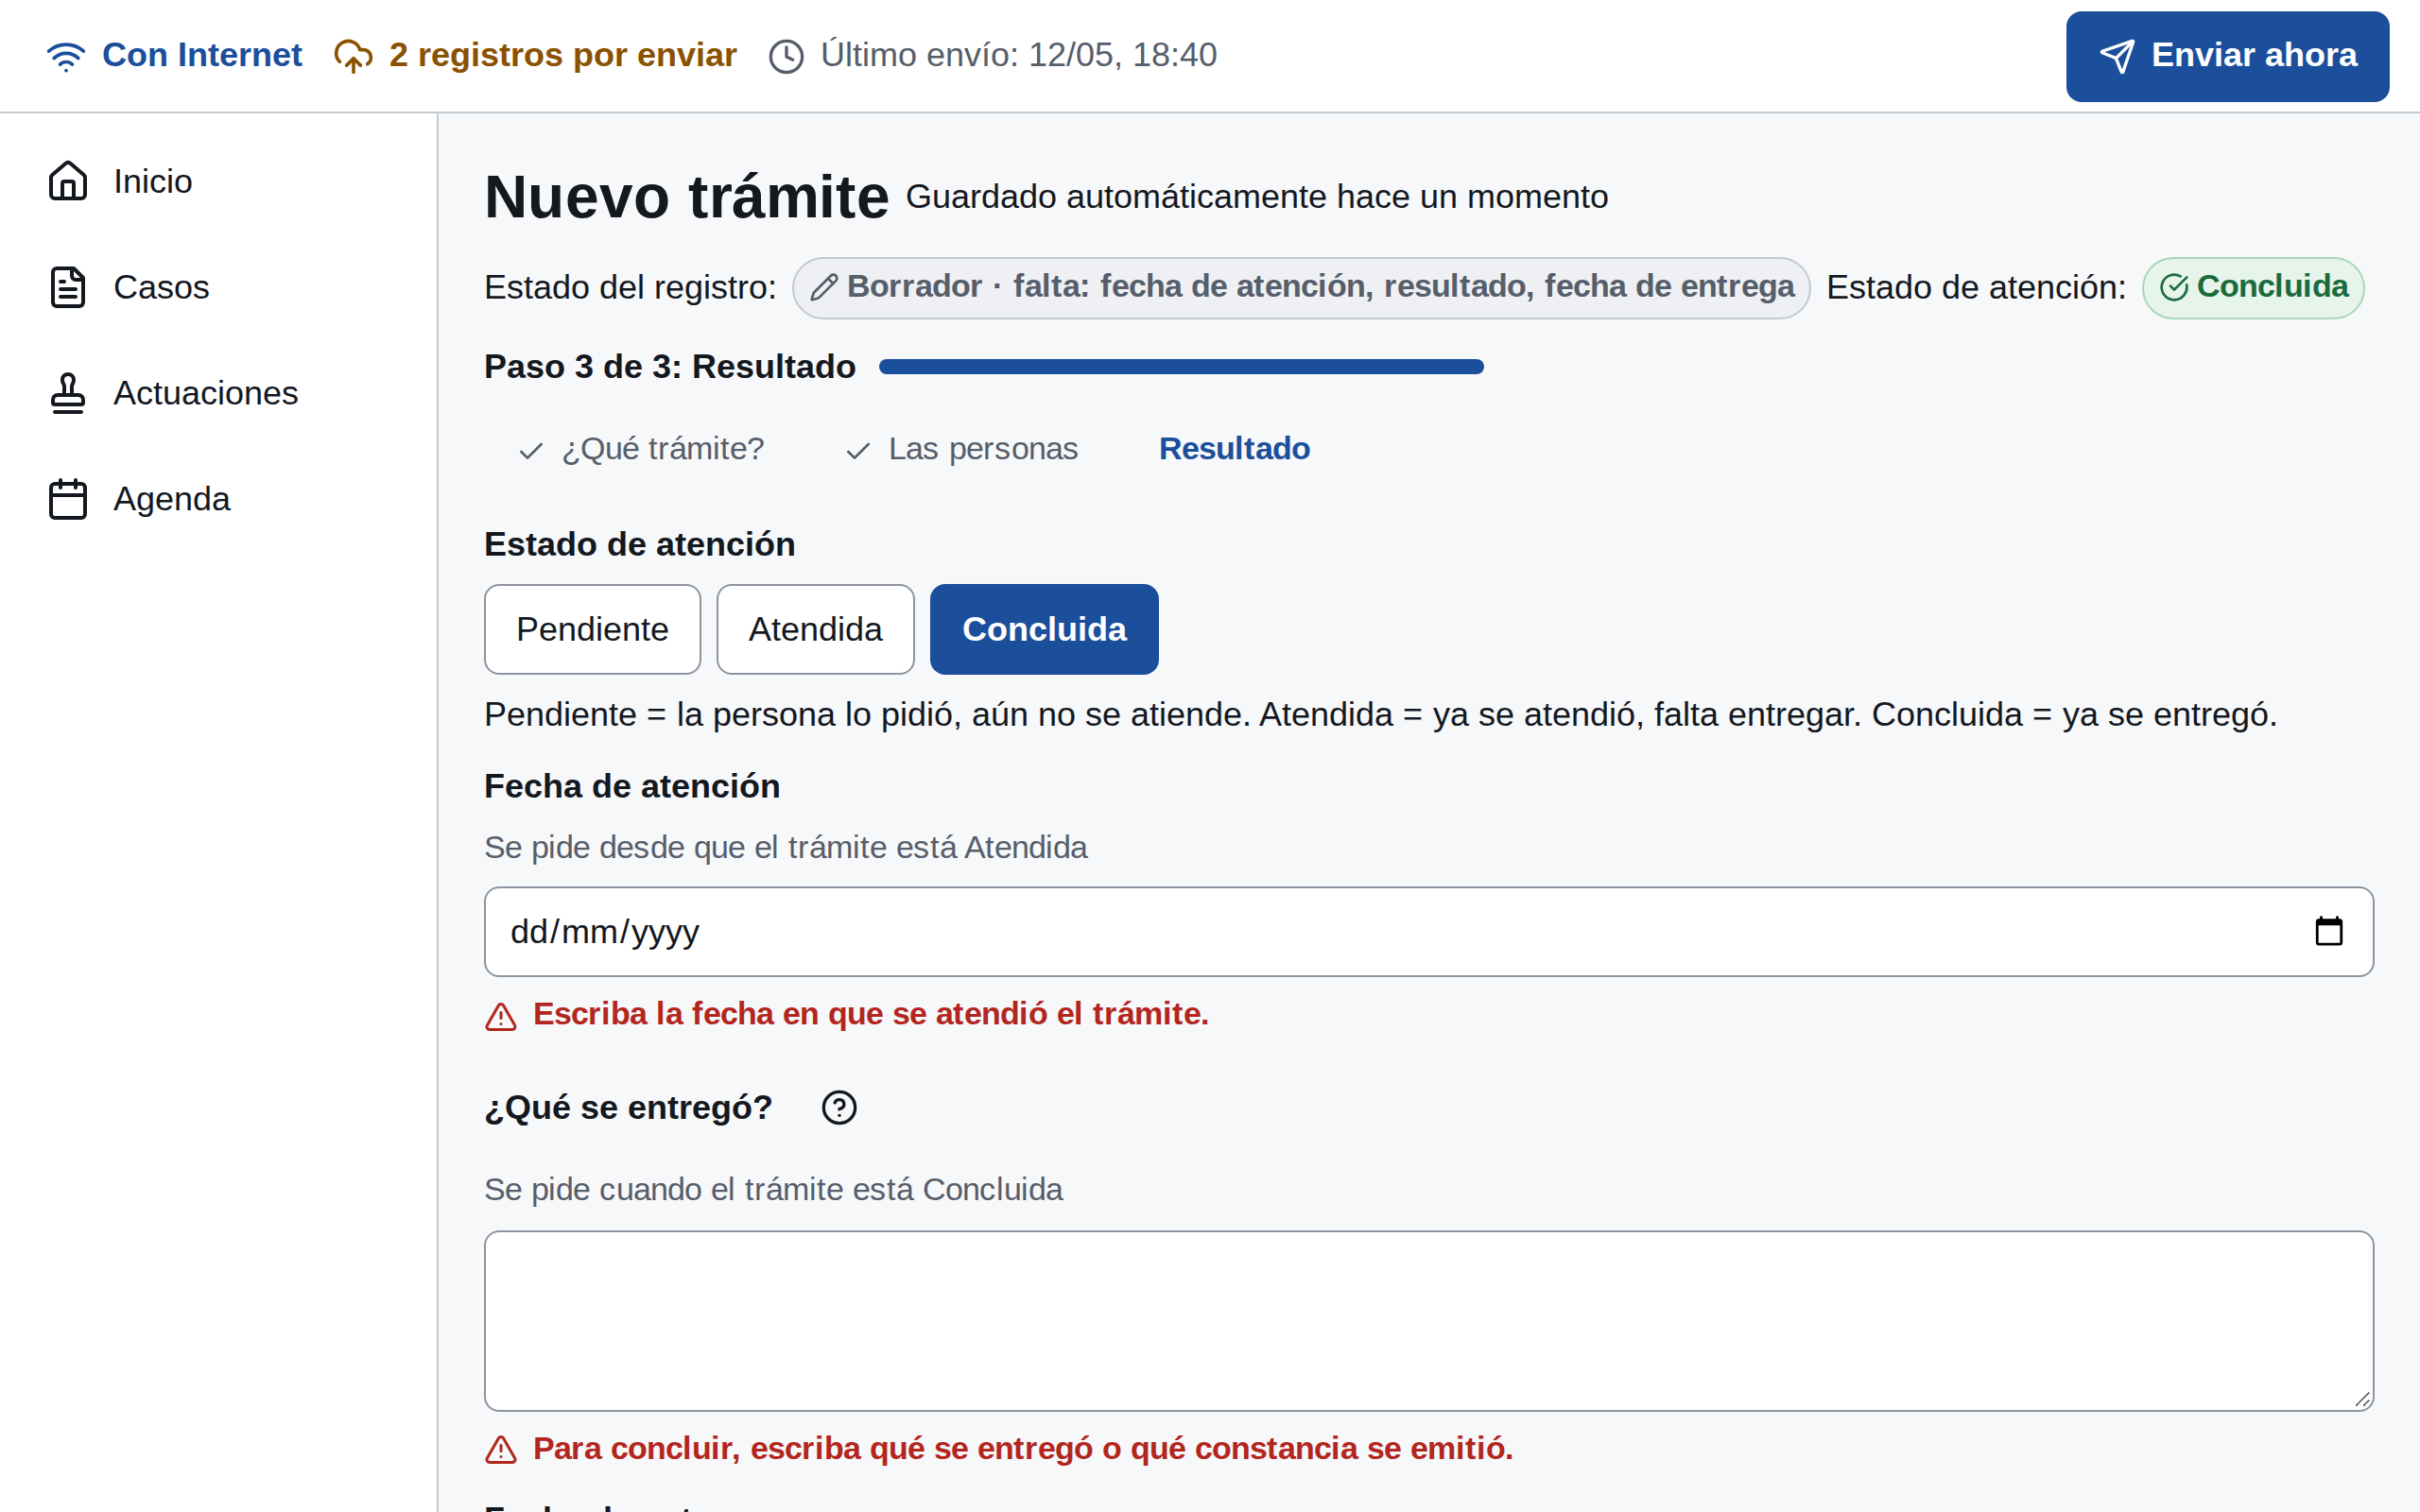
\includegraphics[width=0.82\linewidth]{capturas/F2-06_error-condicional.png}
\caption{P-06 · 4. Error de campo condicional. No deja concluir sin decir qué se entregó, y lo explica en una frase}
\end{figure}
\begin{figure}[H]\centering
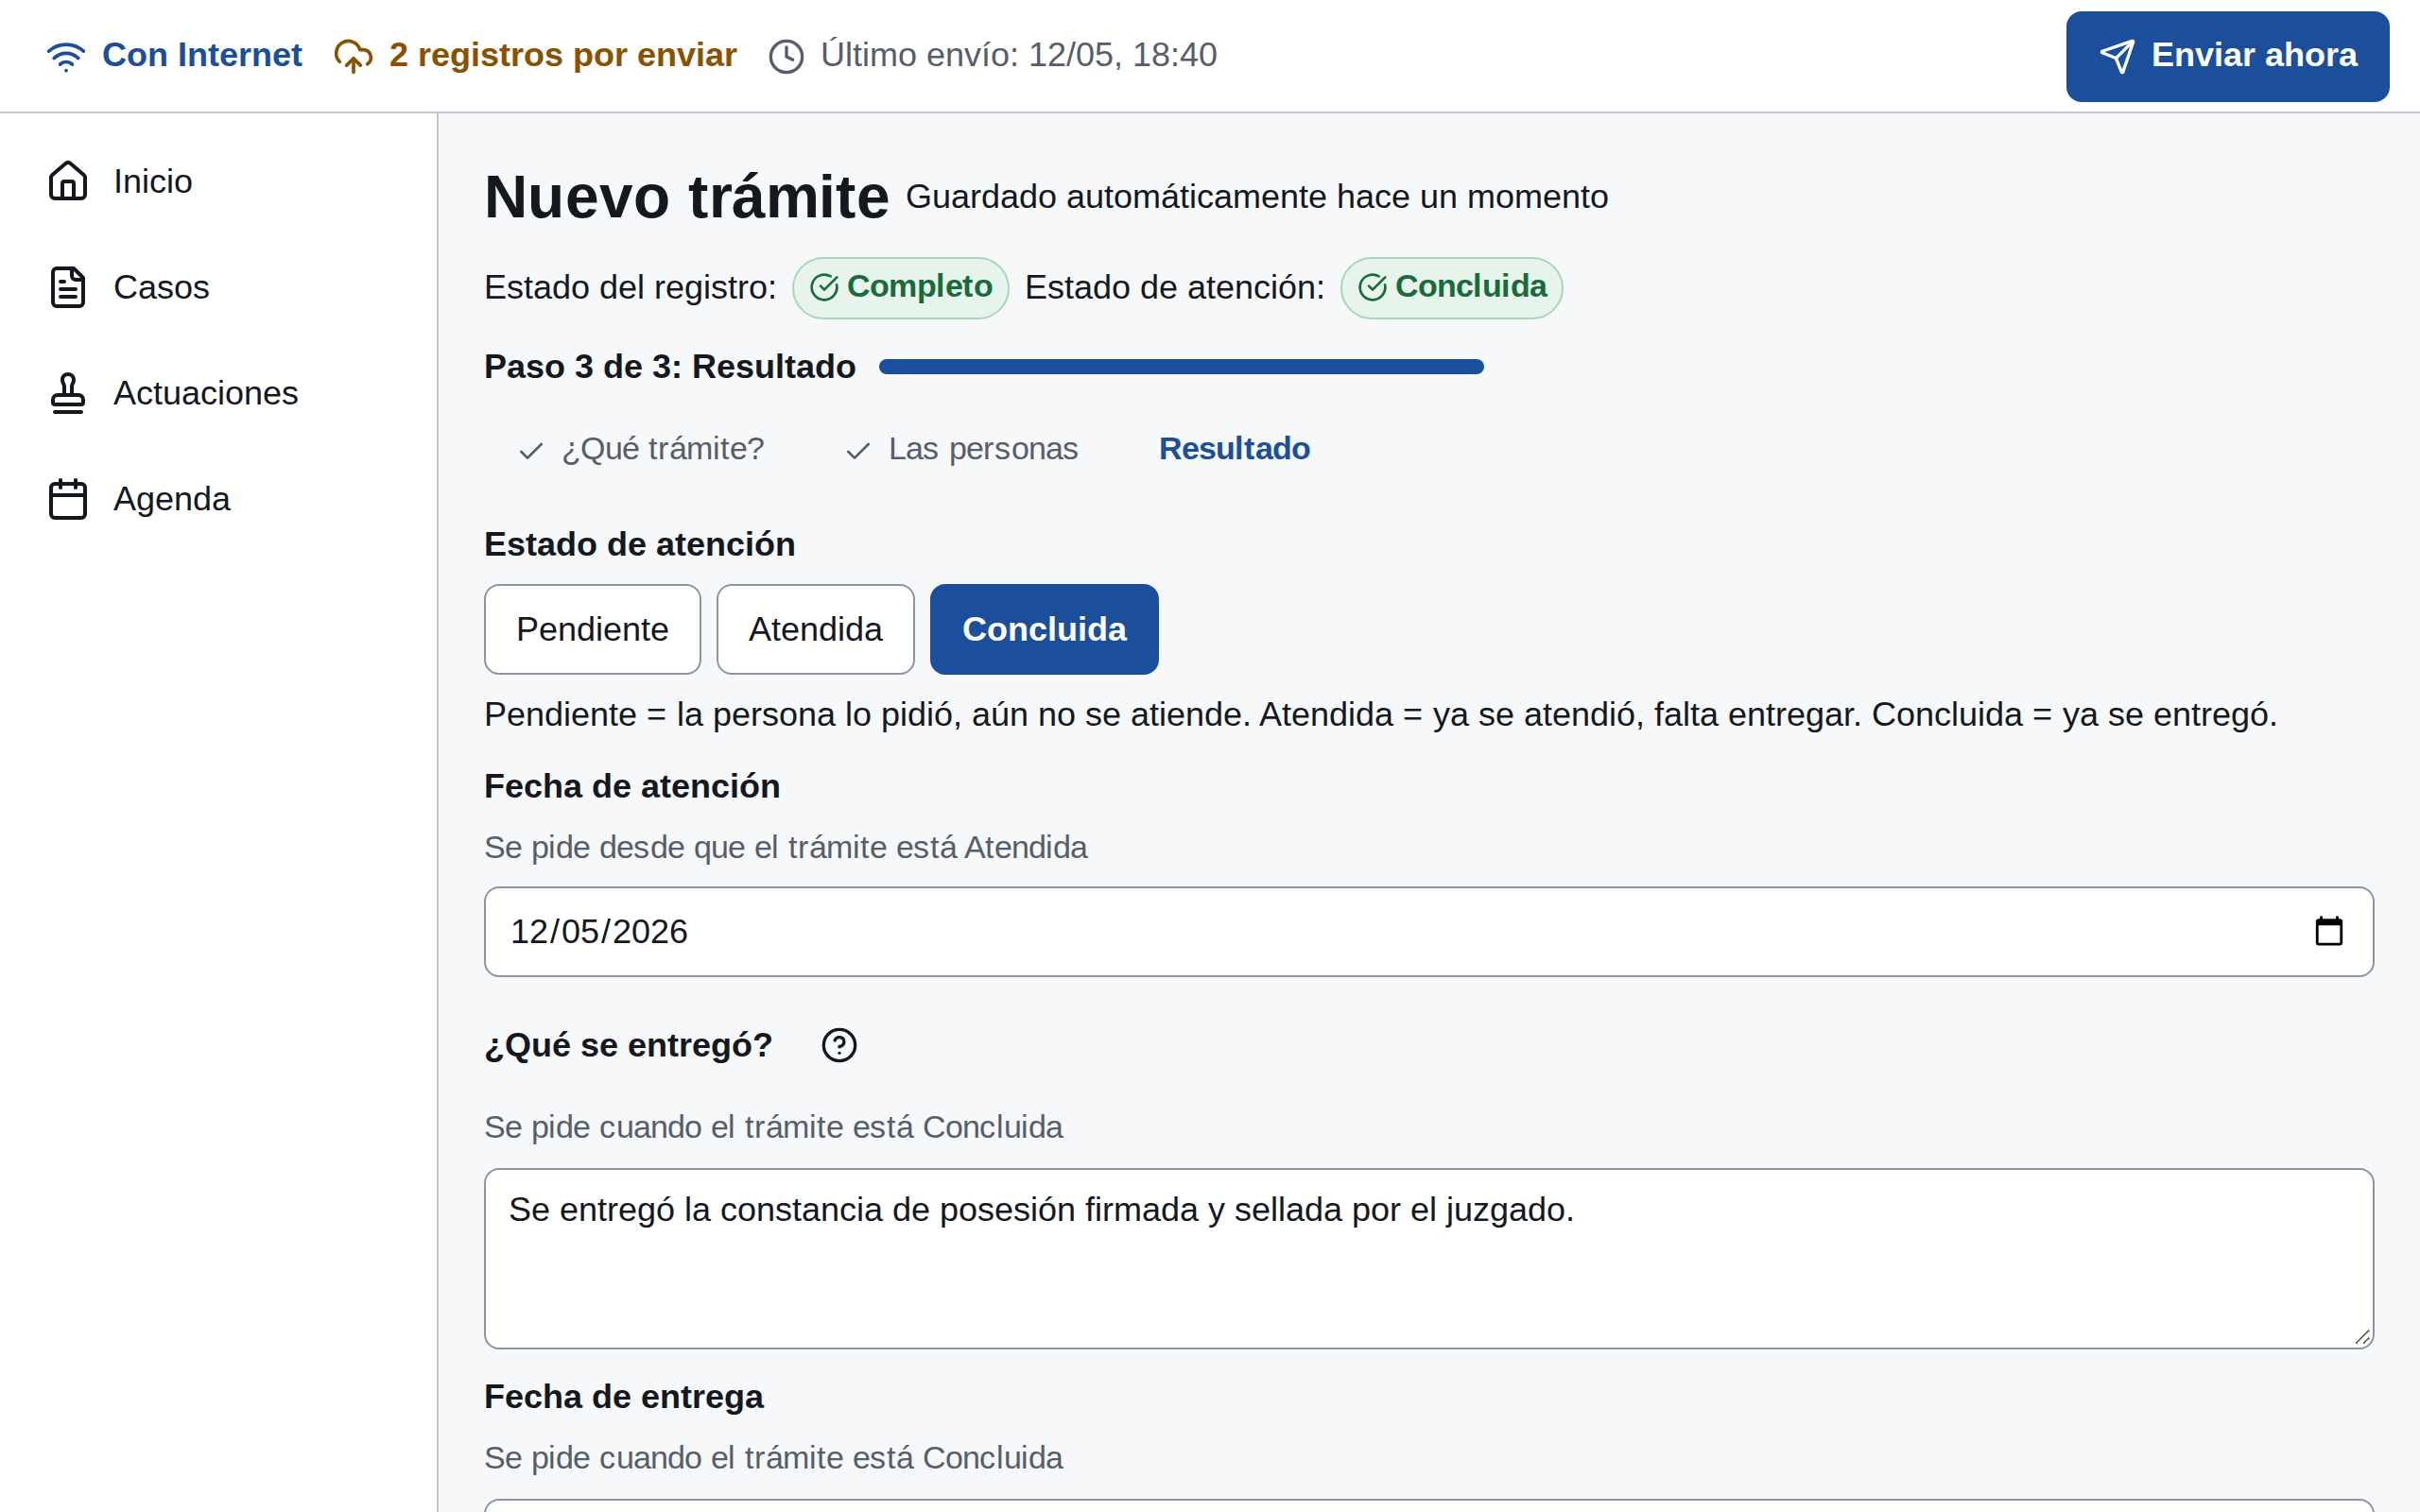
\includegraphics[width=0.82\linewidth]{capturas/F2-07_completo.png}
\caption{P-06 · 5. De Borrador a Completo. El estado del registro pasa a Completo, separado del estado de atención}
\end{figure}
\begin{figure}[H]\centering
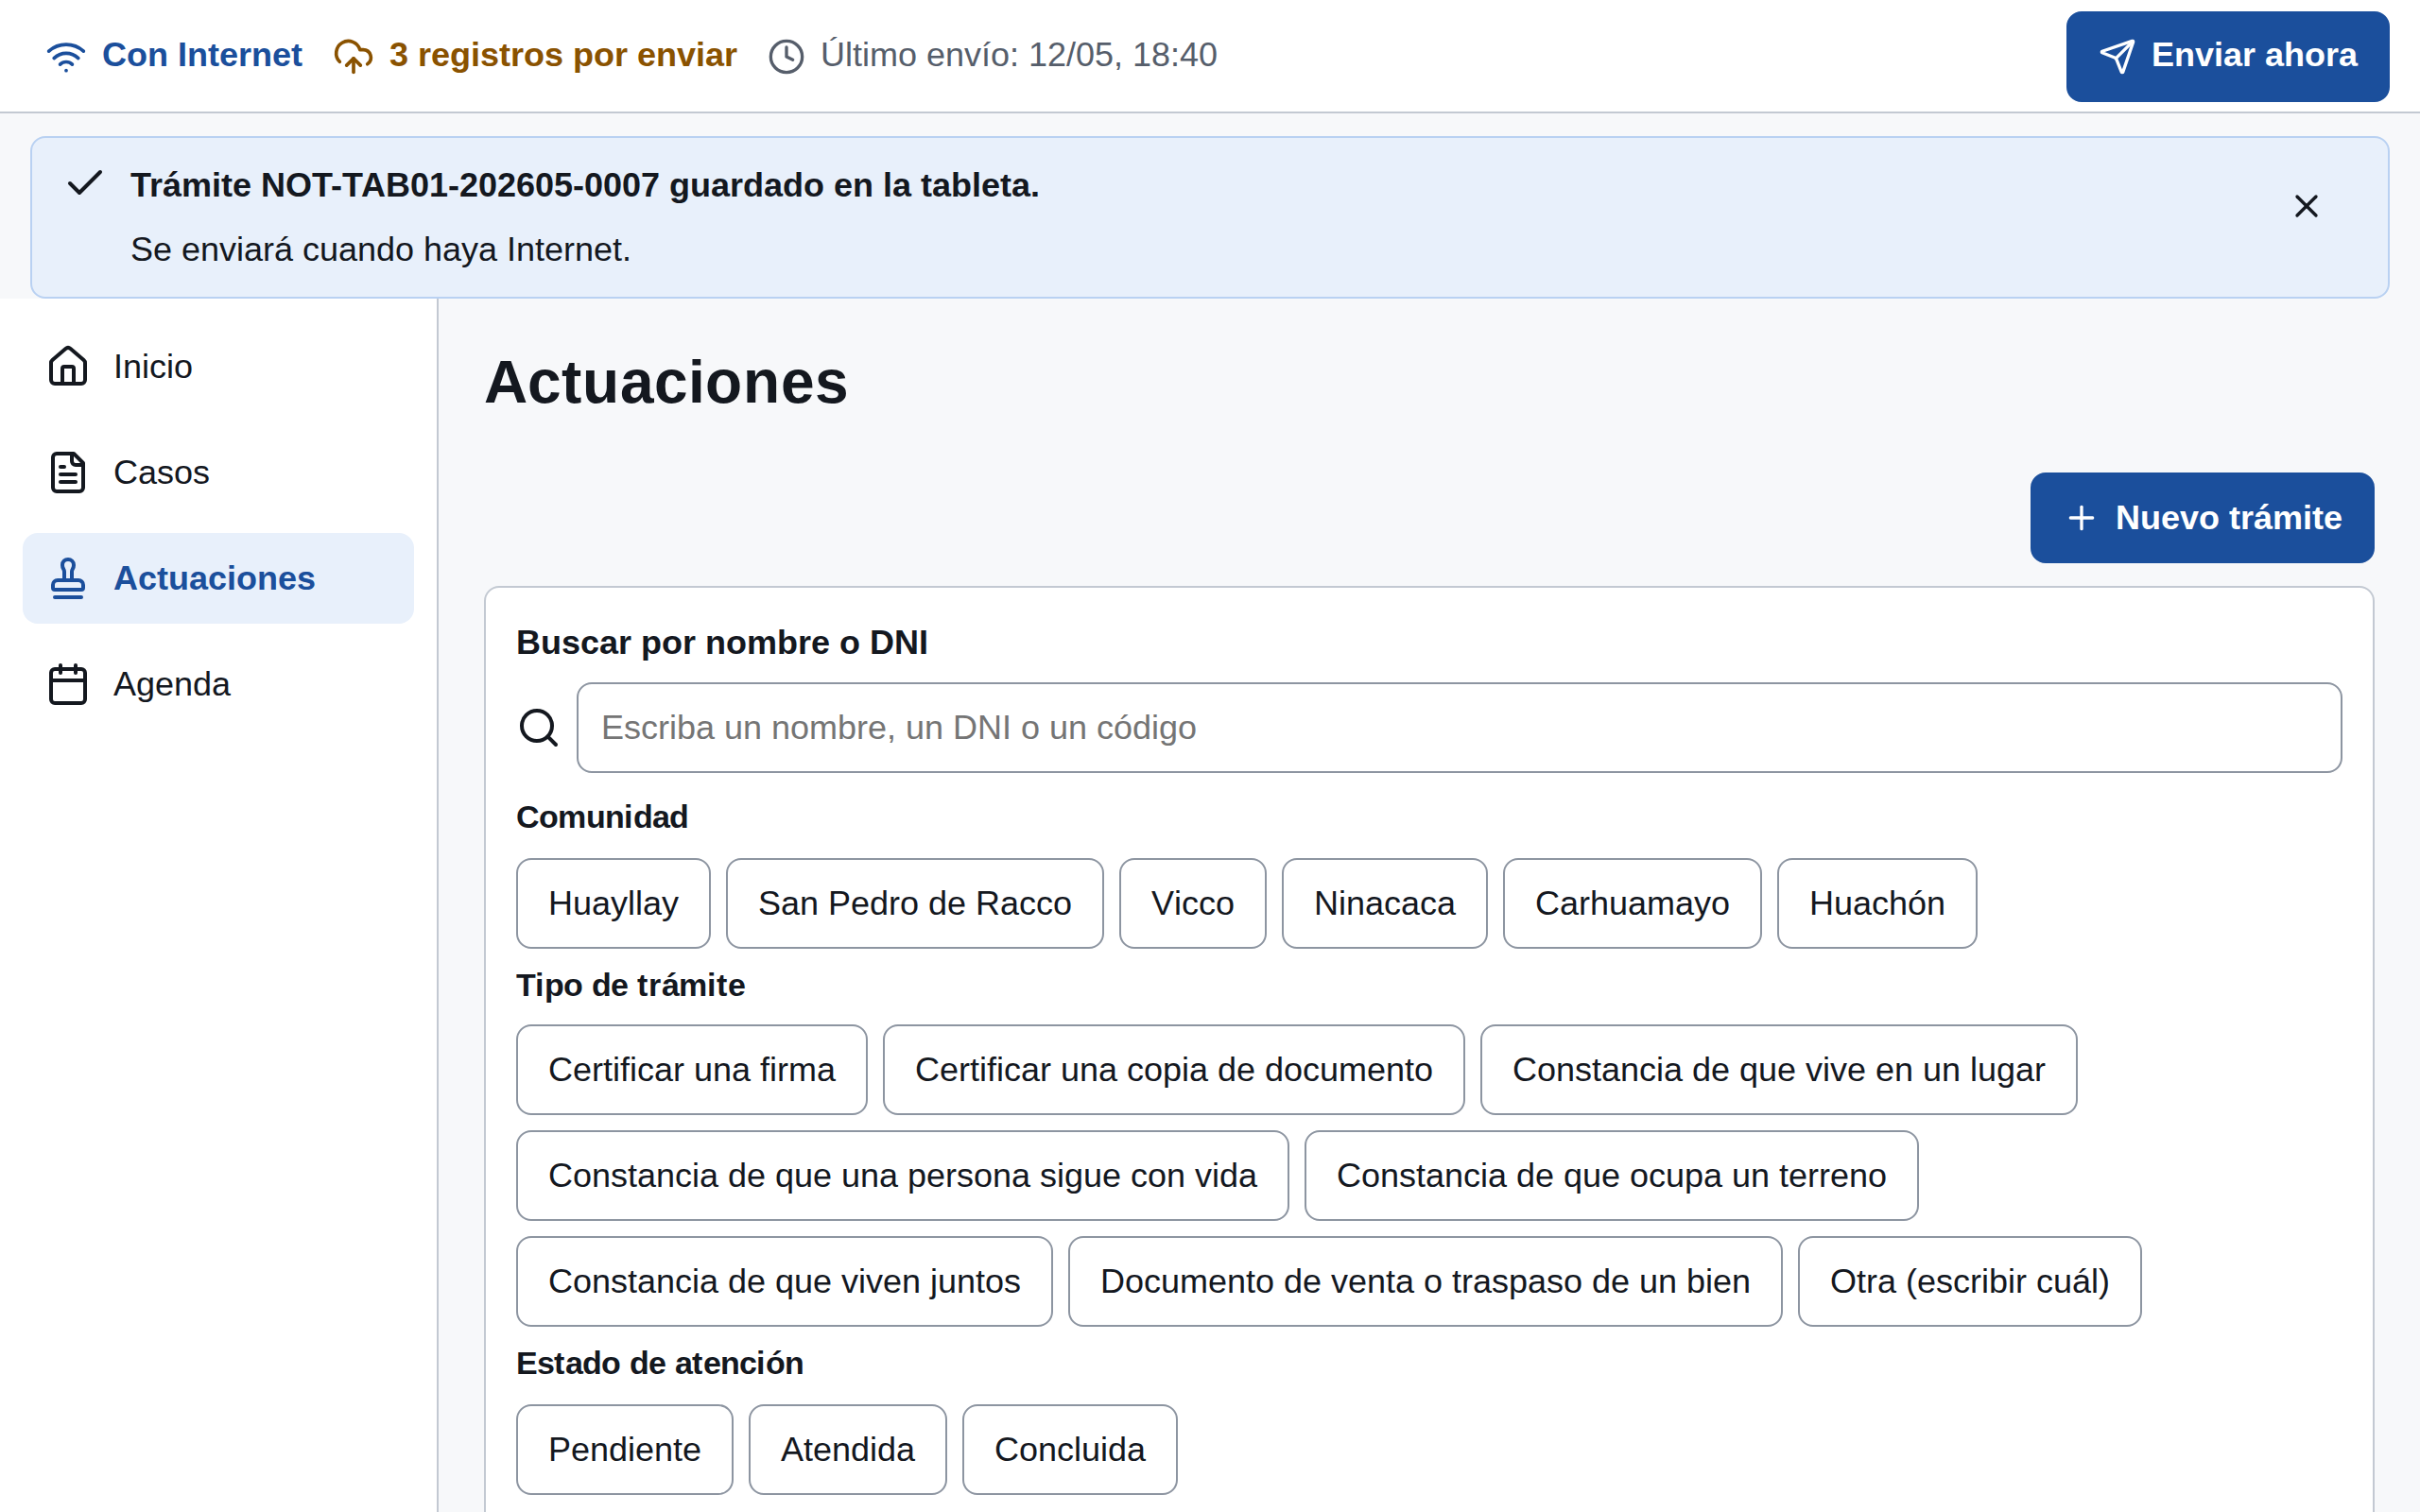
\includegraphics[width=0.82\linewidth]{capturas/F2-08_confirmacion.png}
\caption{P-05 · 6. Confirmación en la tableta. La confirmación dice dónde quedó el trámite y la barra sube su contador a 3}
\end{figure}
\subsection{Flujo 3 · Revisar las actividades de la semana}
\begin{figure}[H]\centering
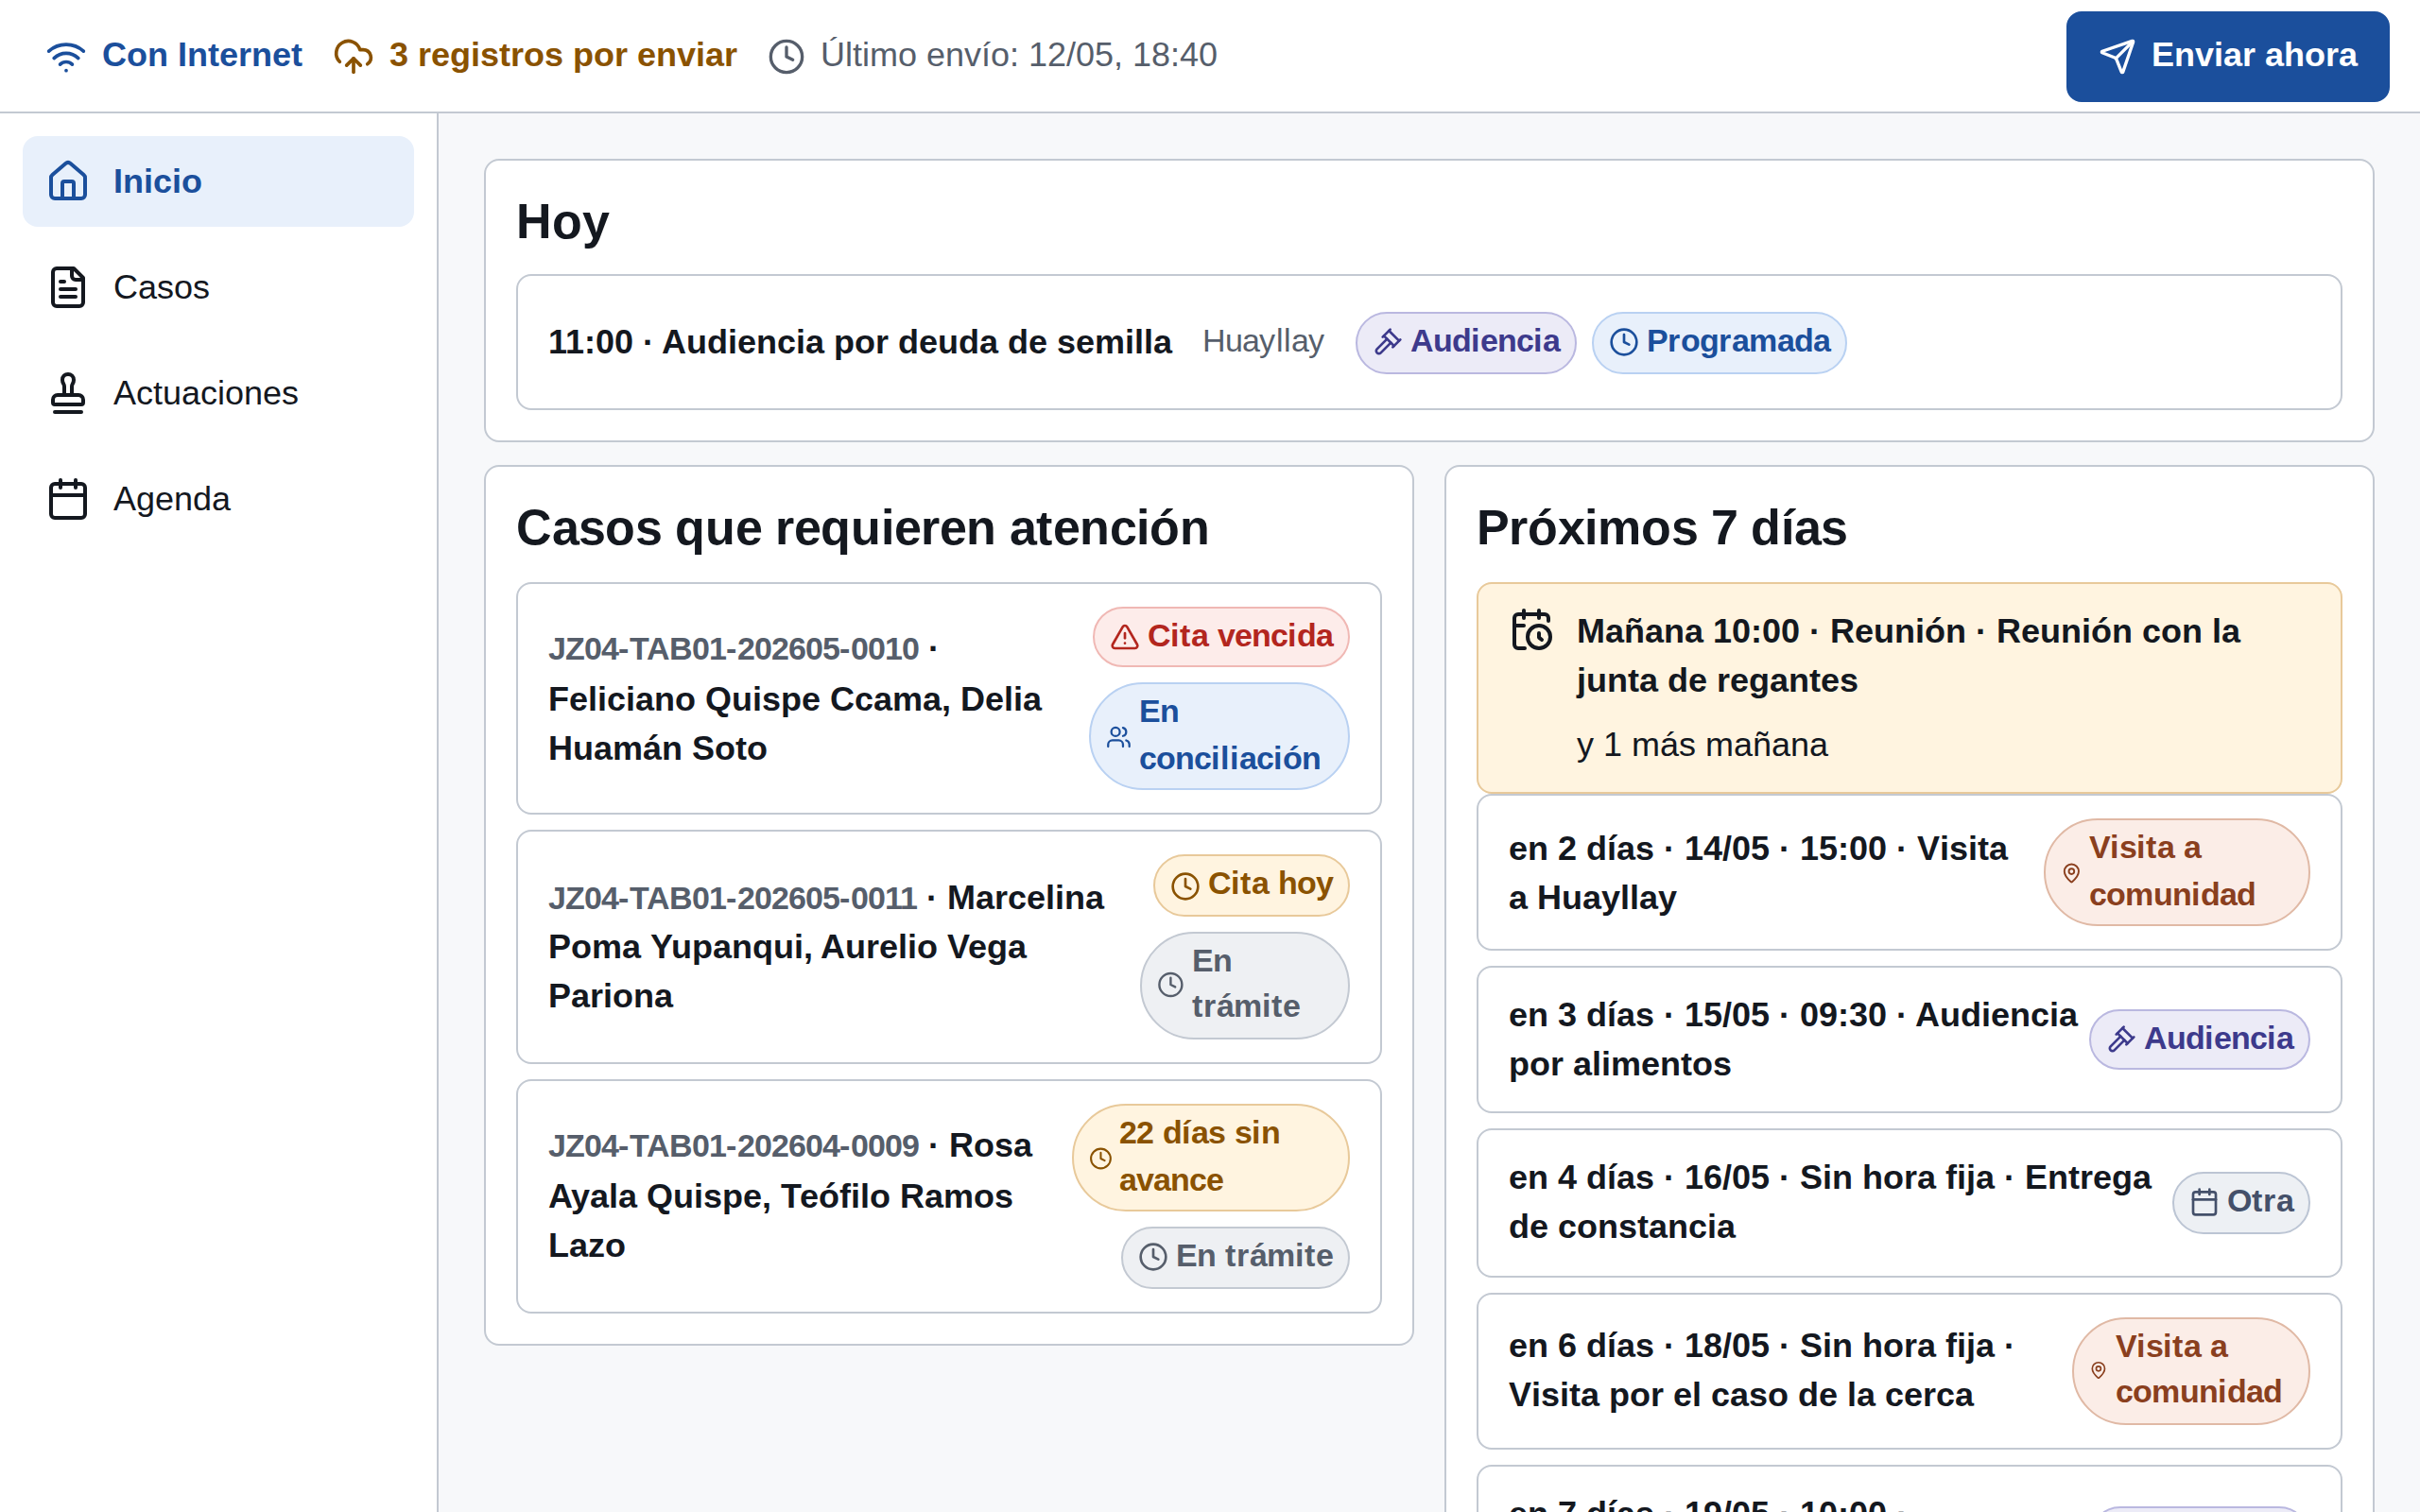
\includegraphics[width=0.82\linewidth]{capturas/F3-01_aviso-manana.png}
\caption{P-01 · 1. Aviso de lo de mañana. El aviso de mañana aparece sin que la jueza tenga que ir a buscarlo}
\end{figure}
\begin{figure}[H]\centering
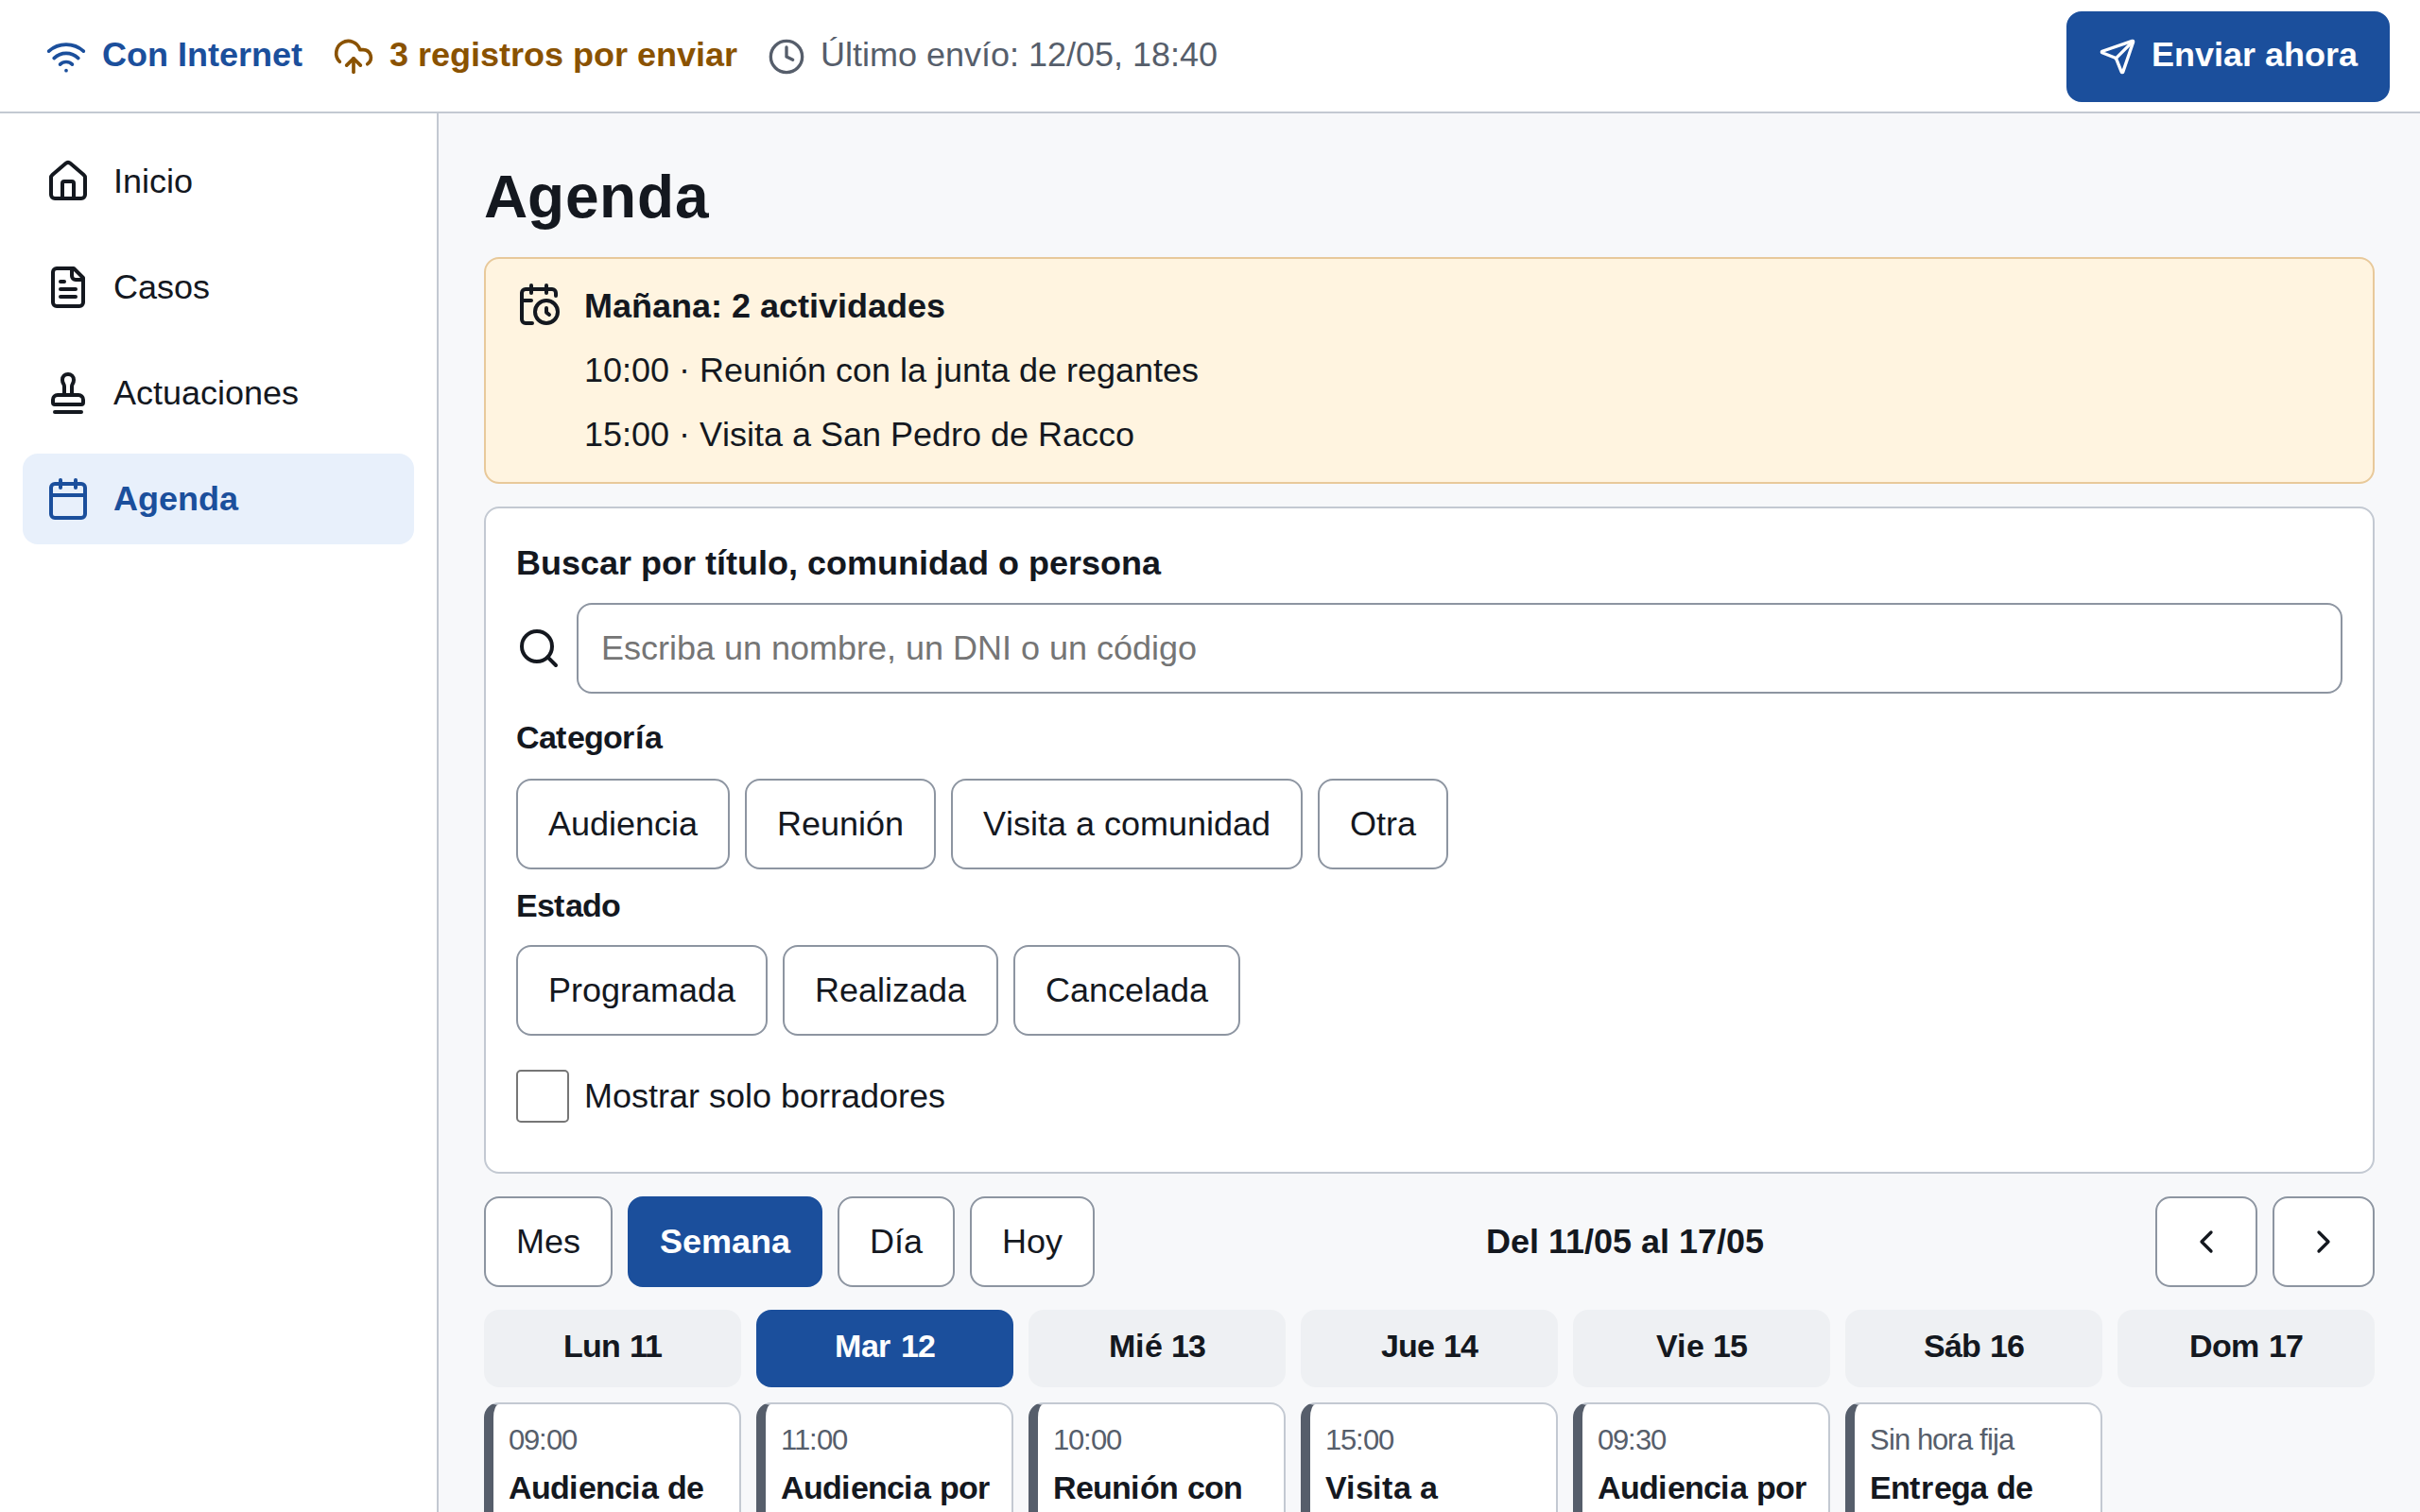
\includegraphics[width=0.82\linewidth]{capturas/F3-02_agenda-semana.png}
\caption{P-07 · 2. Vista semana. Categorías con color, ícono y texto; estados de cada actividad}
\end{figure}
\begin{figure}[H]\centering
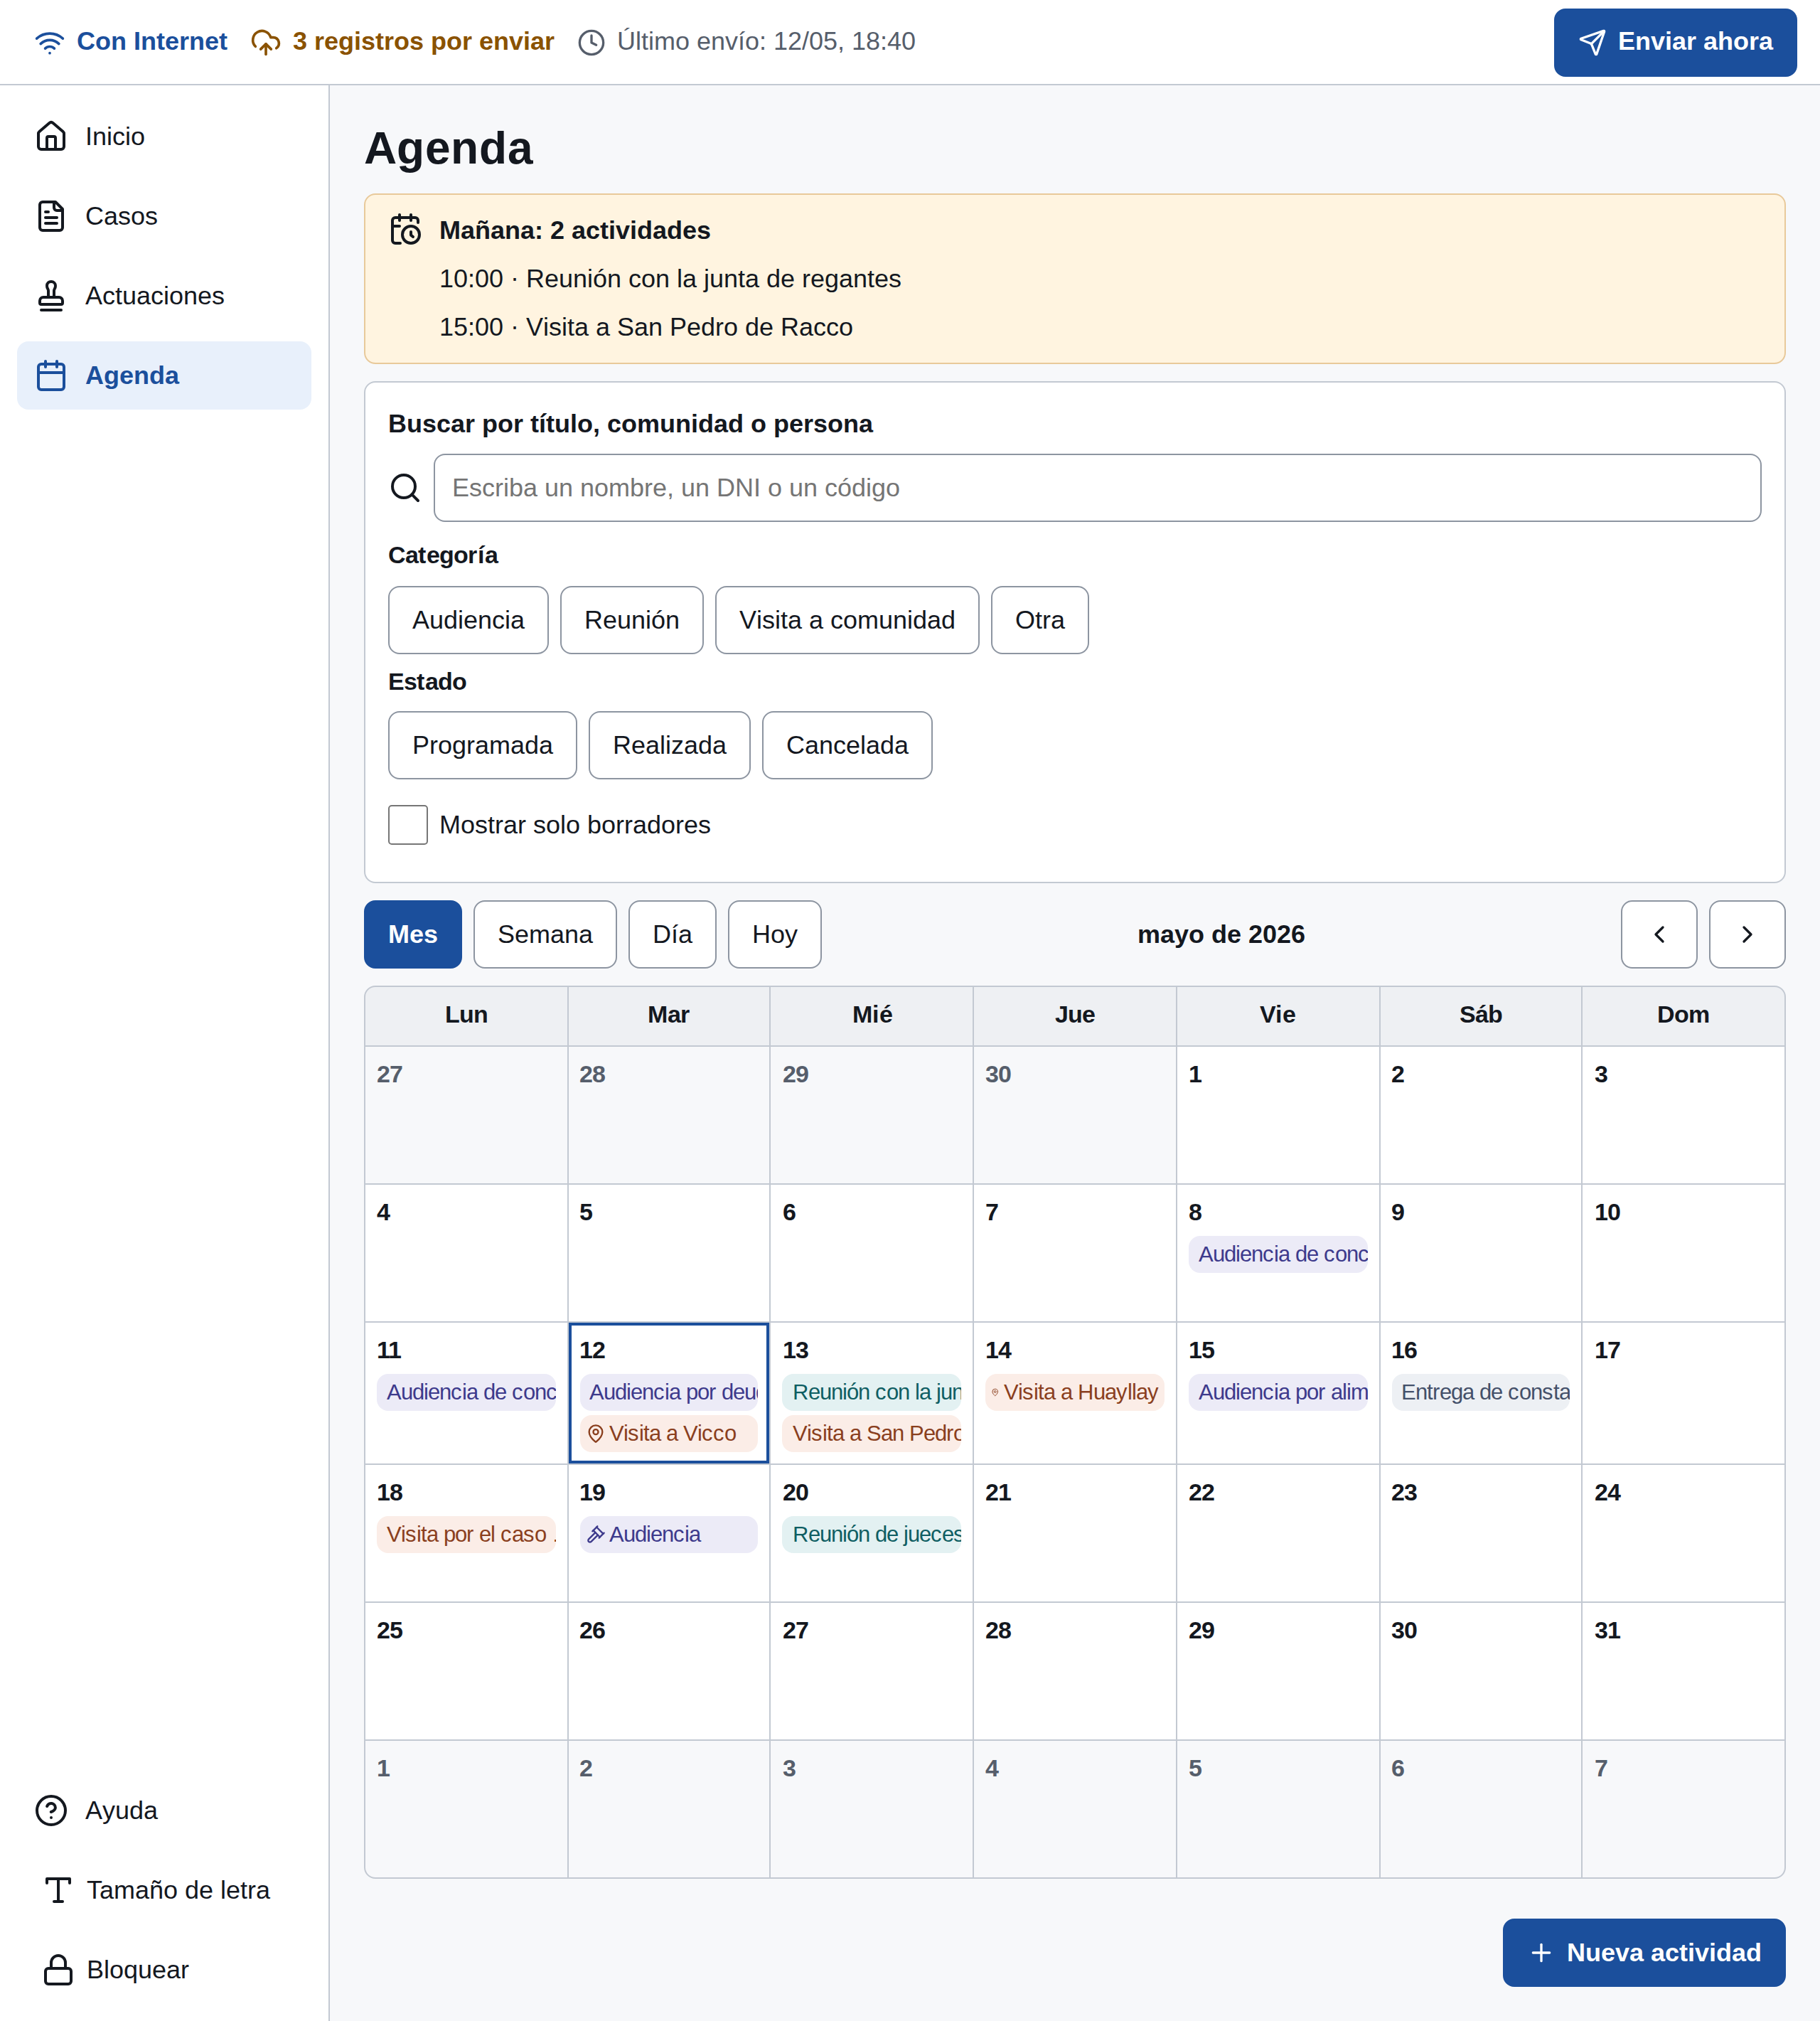
\includegraphics[width=0.82\linewidth]{capturas/F3-03_agenda-mes.png}
\caption{P-07 · 2. Vista mes. Vista mes con las actividades de cada día en píldoras de color y texto}
\end{figure}
\begin{figure}[H]\centering
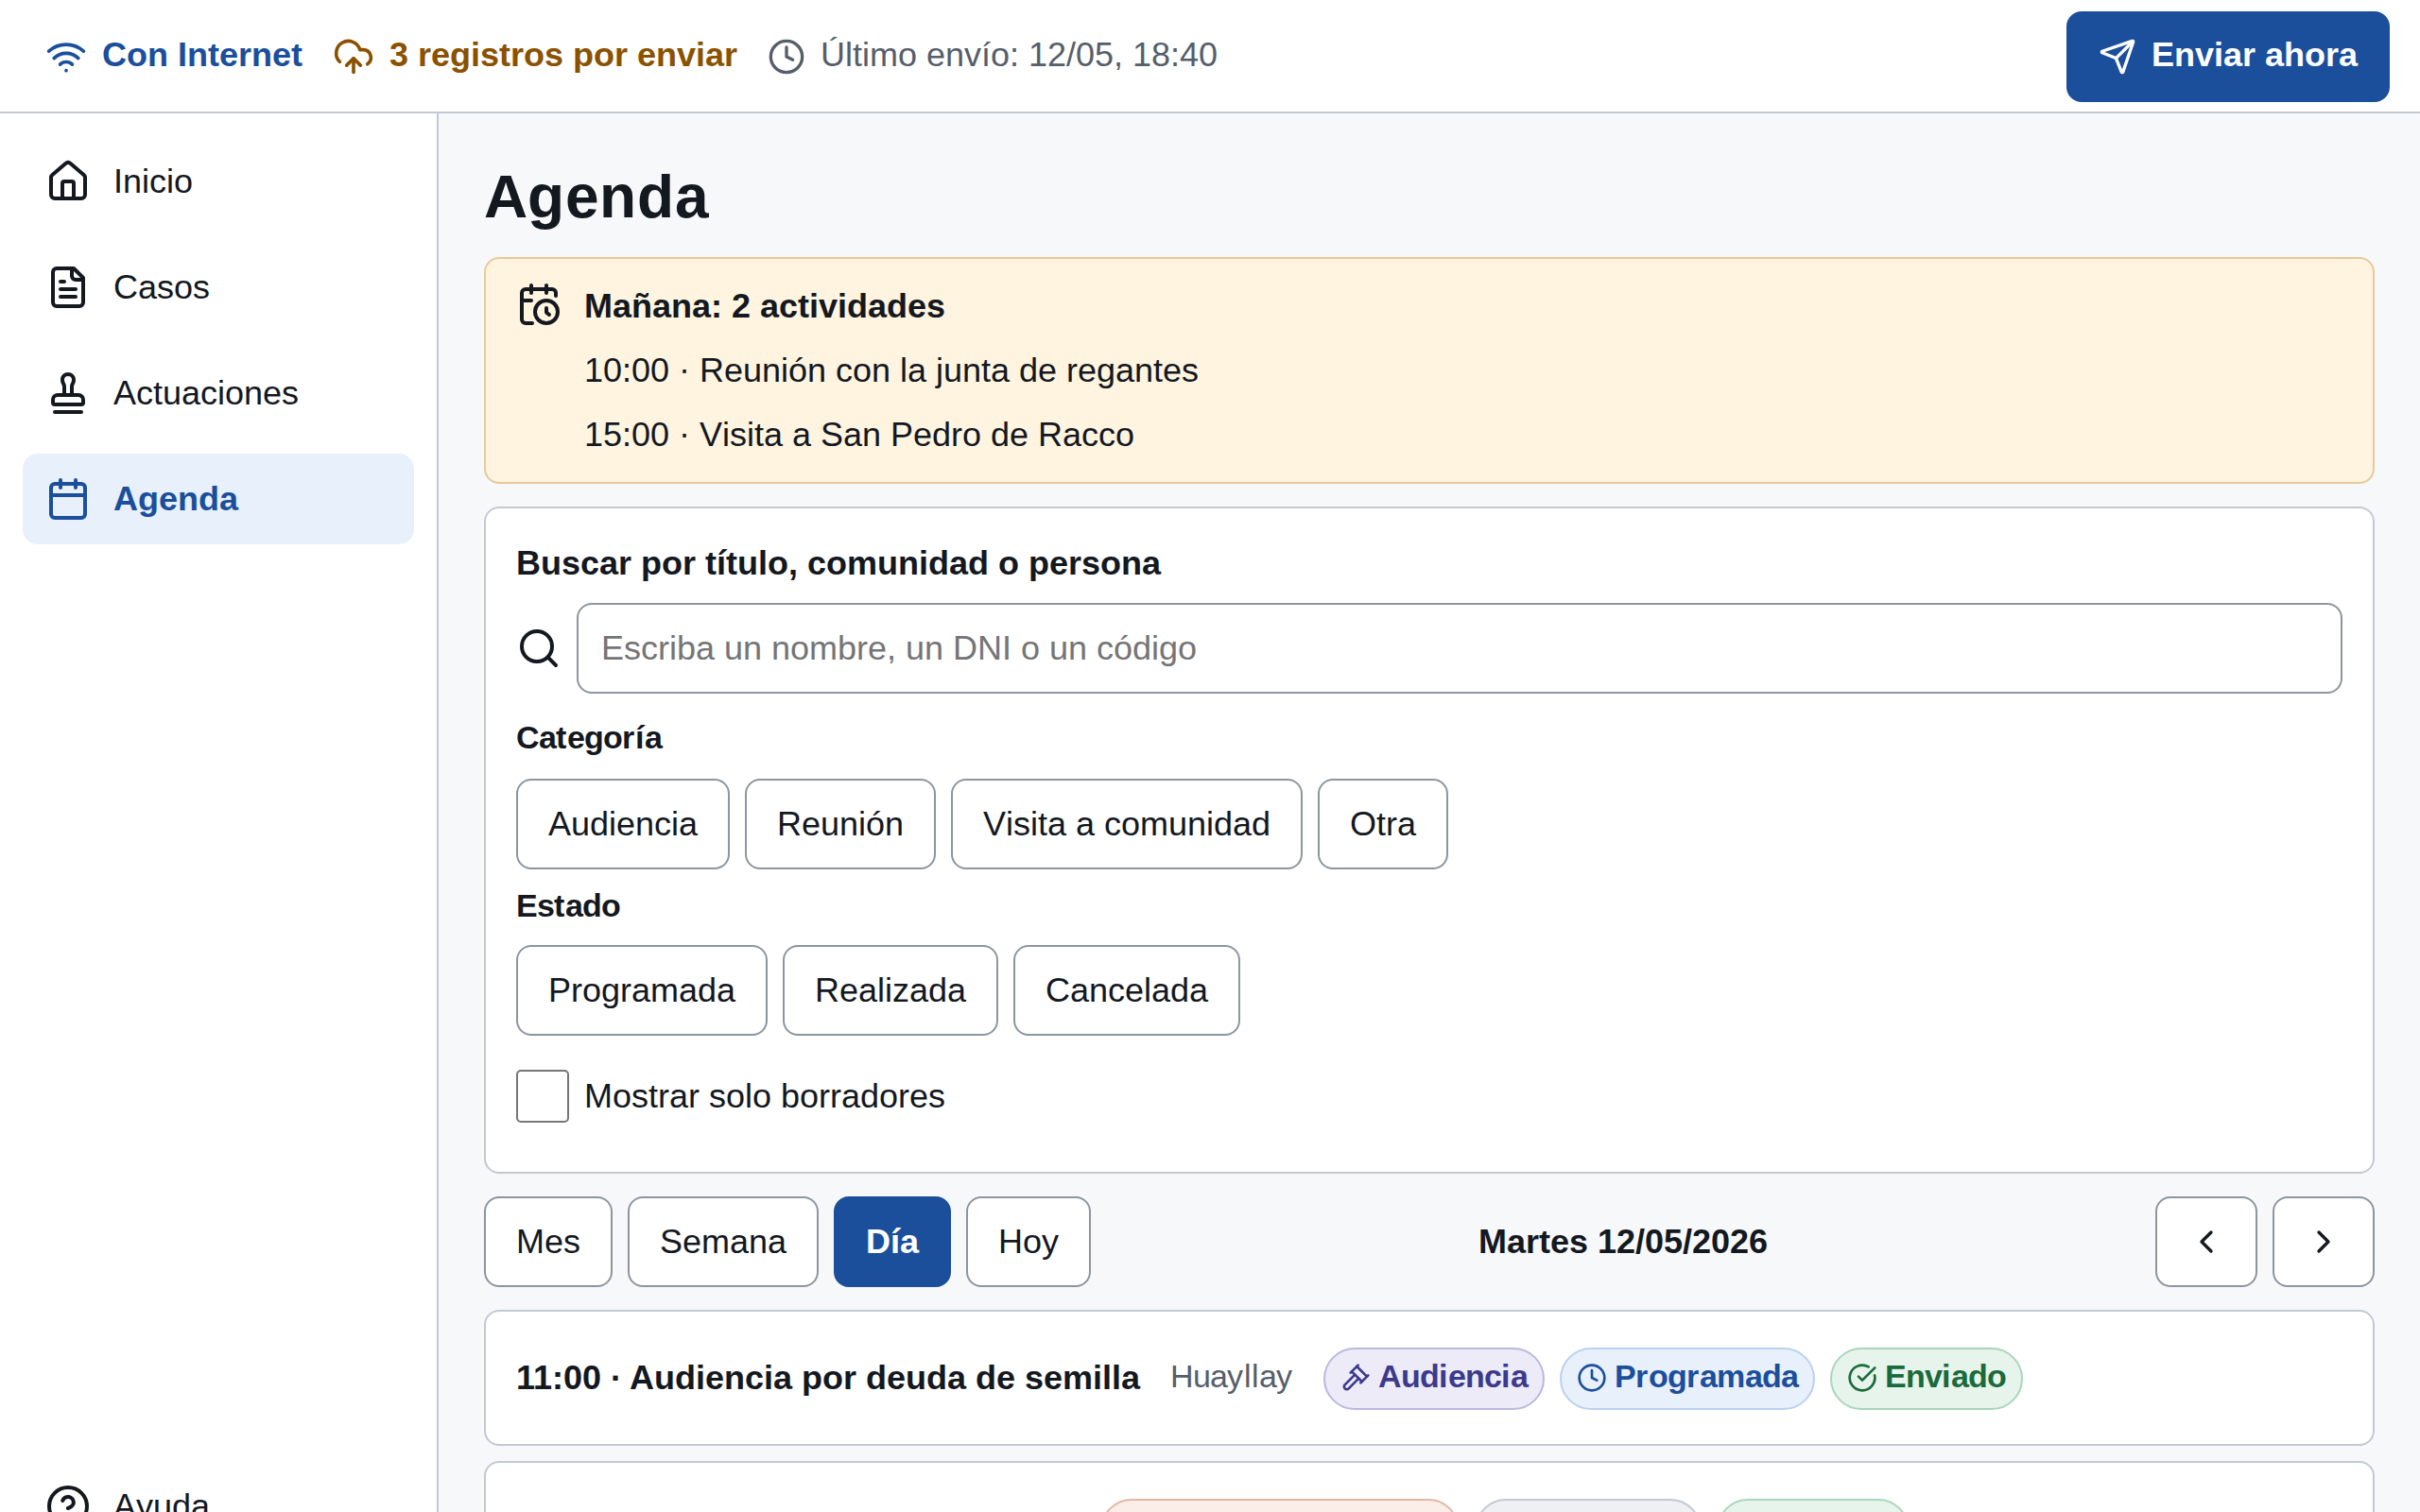
\includegraphics[width=0.82\linewidth]{capturas/F3-04_agenda-dia.png}
\caption{P-07 · 3. Vista día. Vista día con el detalle de cada actividad}
\end{figure}
\begin{figure}[H]\centering
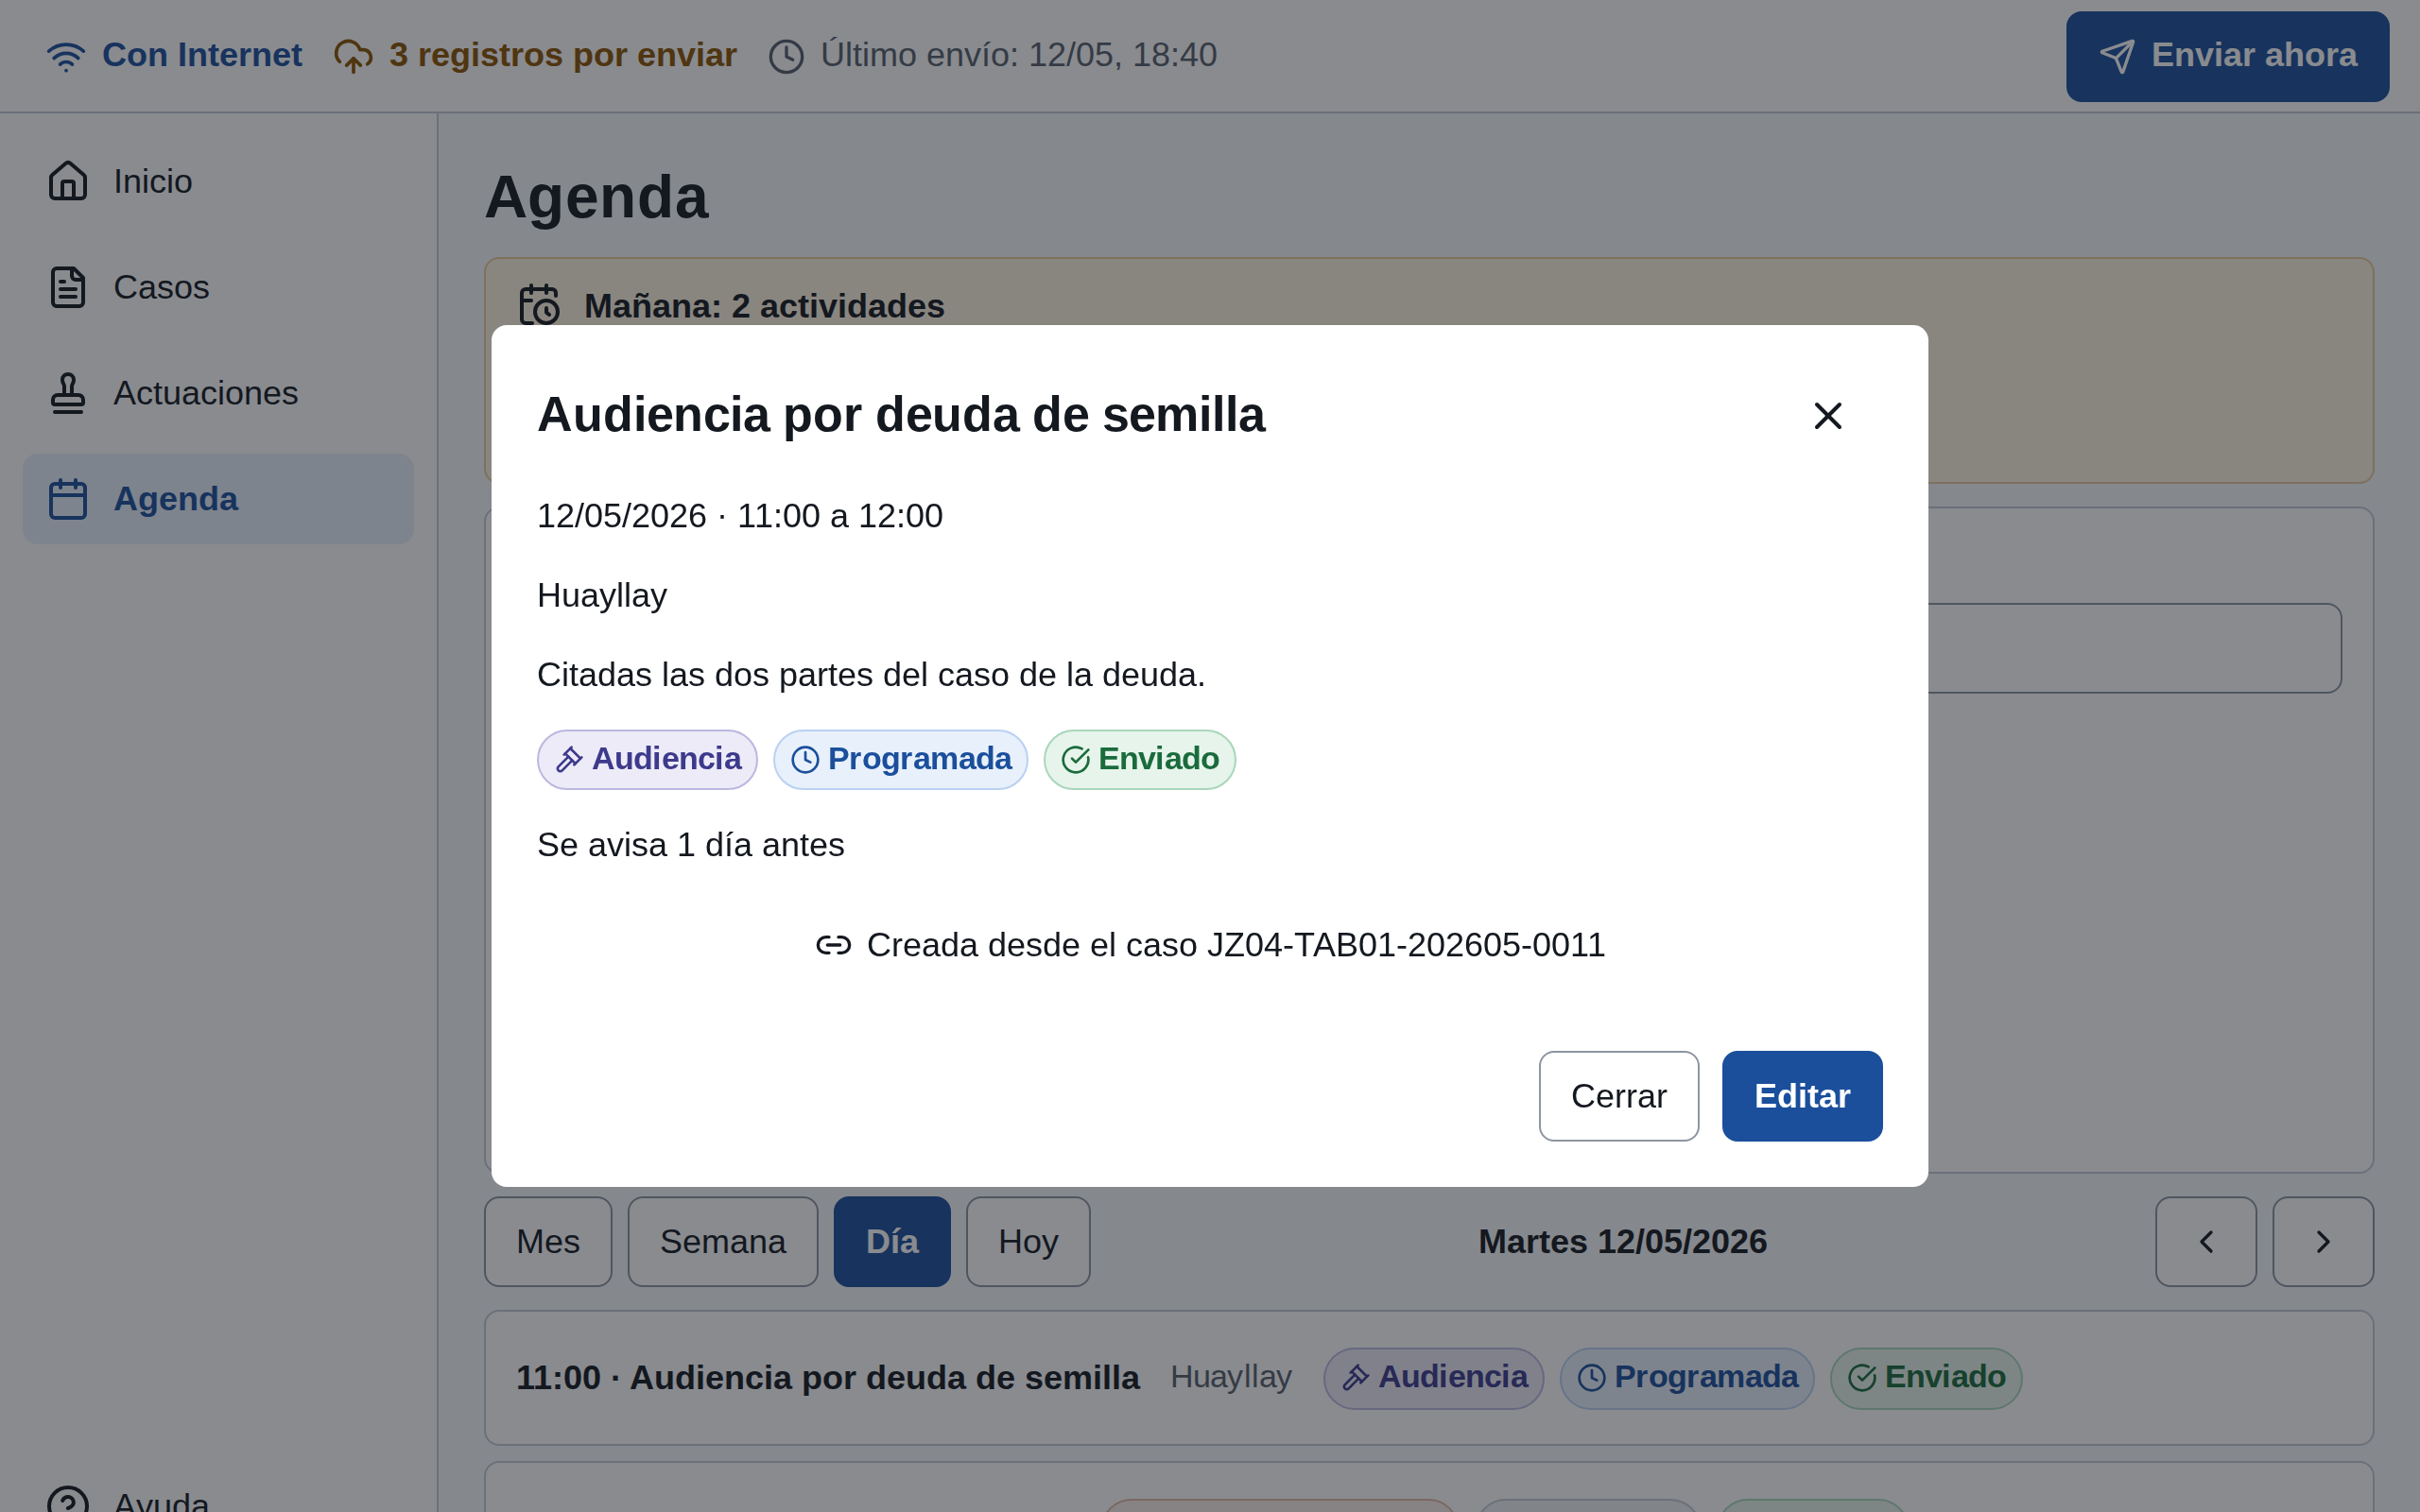
\includegraphics[width=0.82\linewidth]{capturas/F3-05_actividad-detalle.png}
\caption{P-07 · 3. Detalle con su vínculo al caso. La actividad muestra desde qué caso se creó y lleva a él}
\end{figure}
\subsection{Flujo 4 · Agendar una reunión y enviar todo}
\begin{figure}[H]\centering
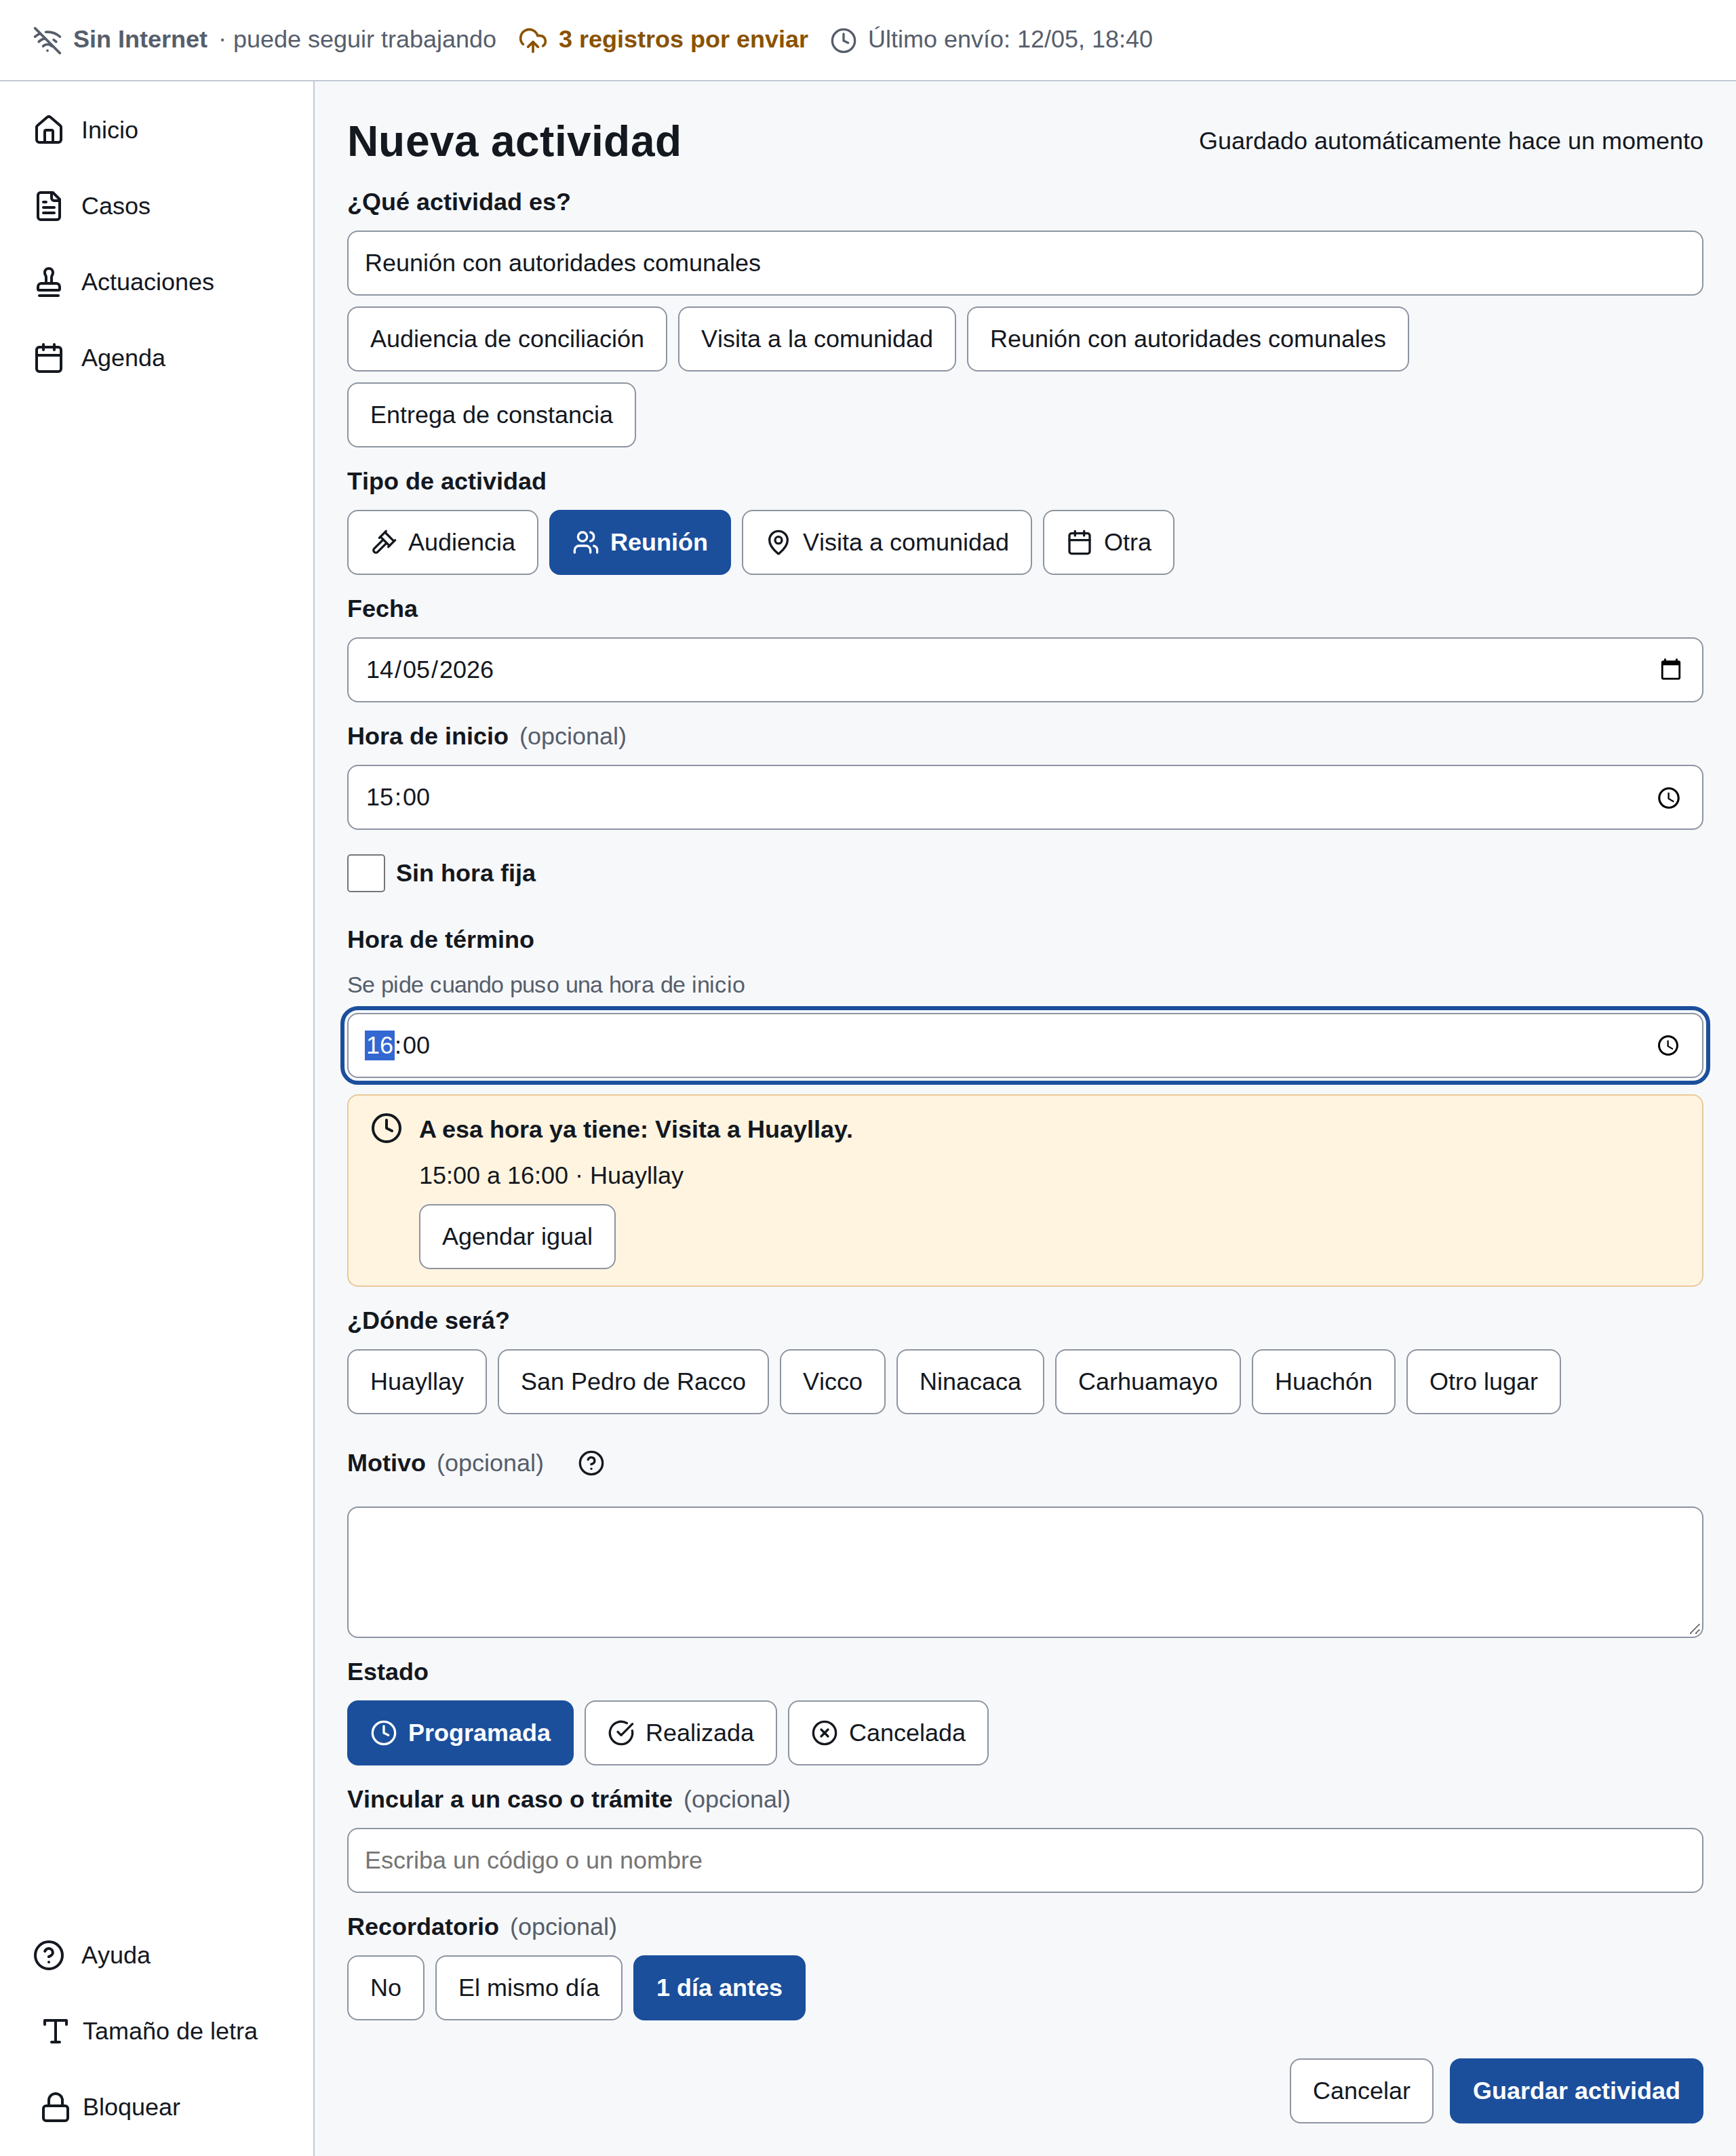
\includegraphics[width=0.82\linewidth]{capturas/F4-01_cruce-horario.png}
\caption{P-08 · 2. Aviso de cruce de horario. Avisa qué actividad choca a esa hora, sin bloquear}
\end{figure}
\begin{figure}[H]\centering
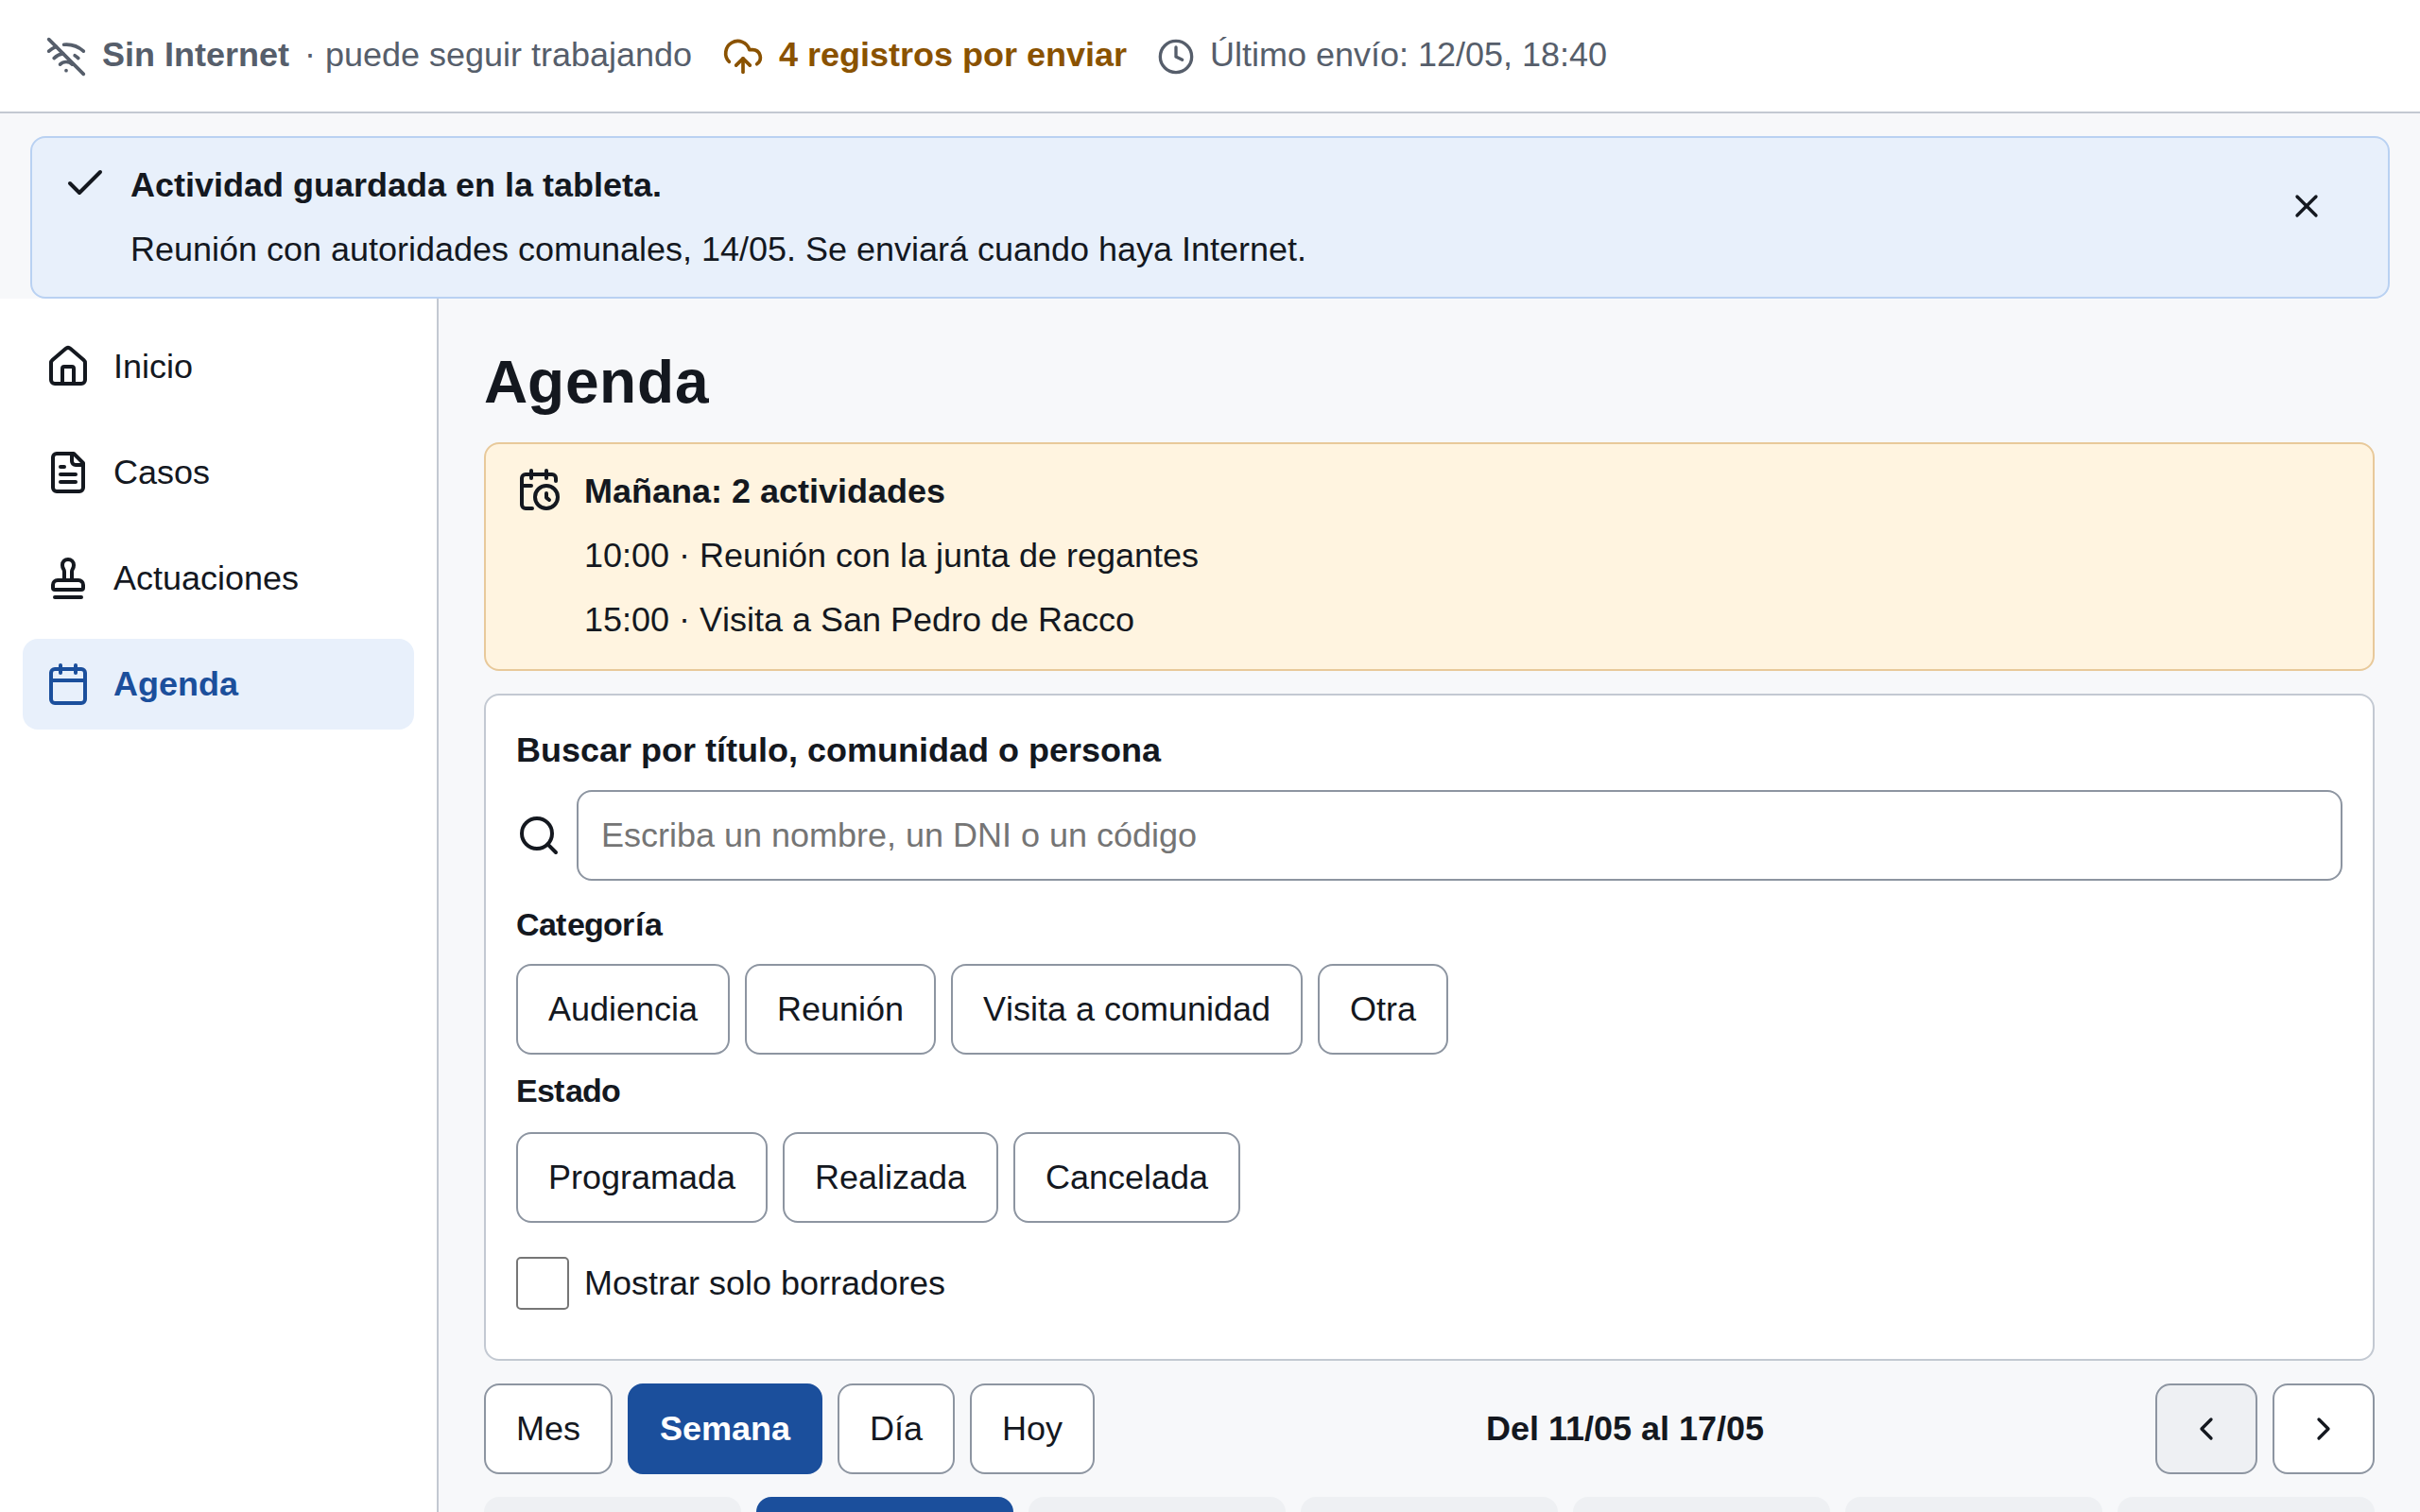
\includegraphics[width=0.82\linewidth]{capturas/F4-02_guardada.png}
\caption{P-07 · 3. Actividad guardada en la tableta. Confirmación de guardado local y contador de la barra en 4}
\end{figure}
\begin{figure}[H]\centering
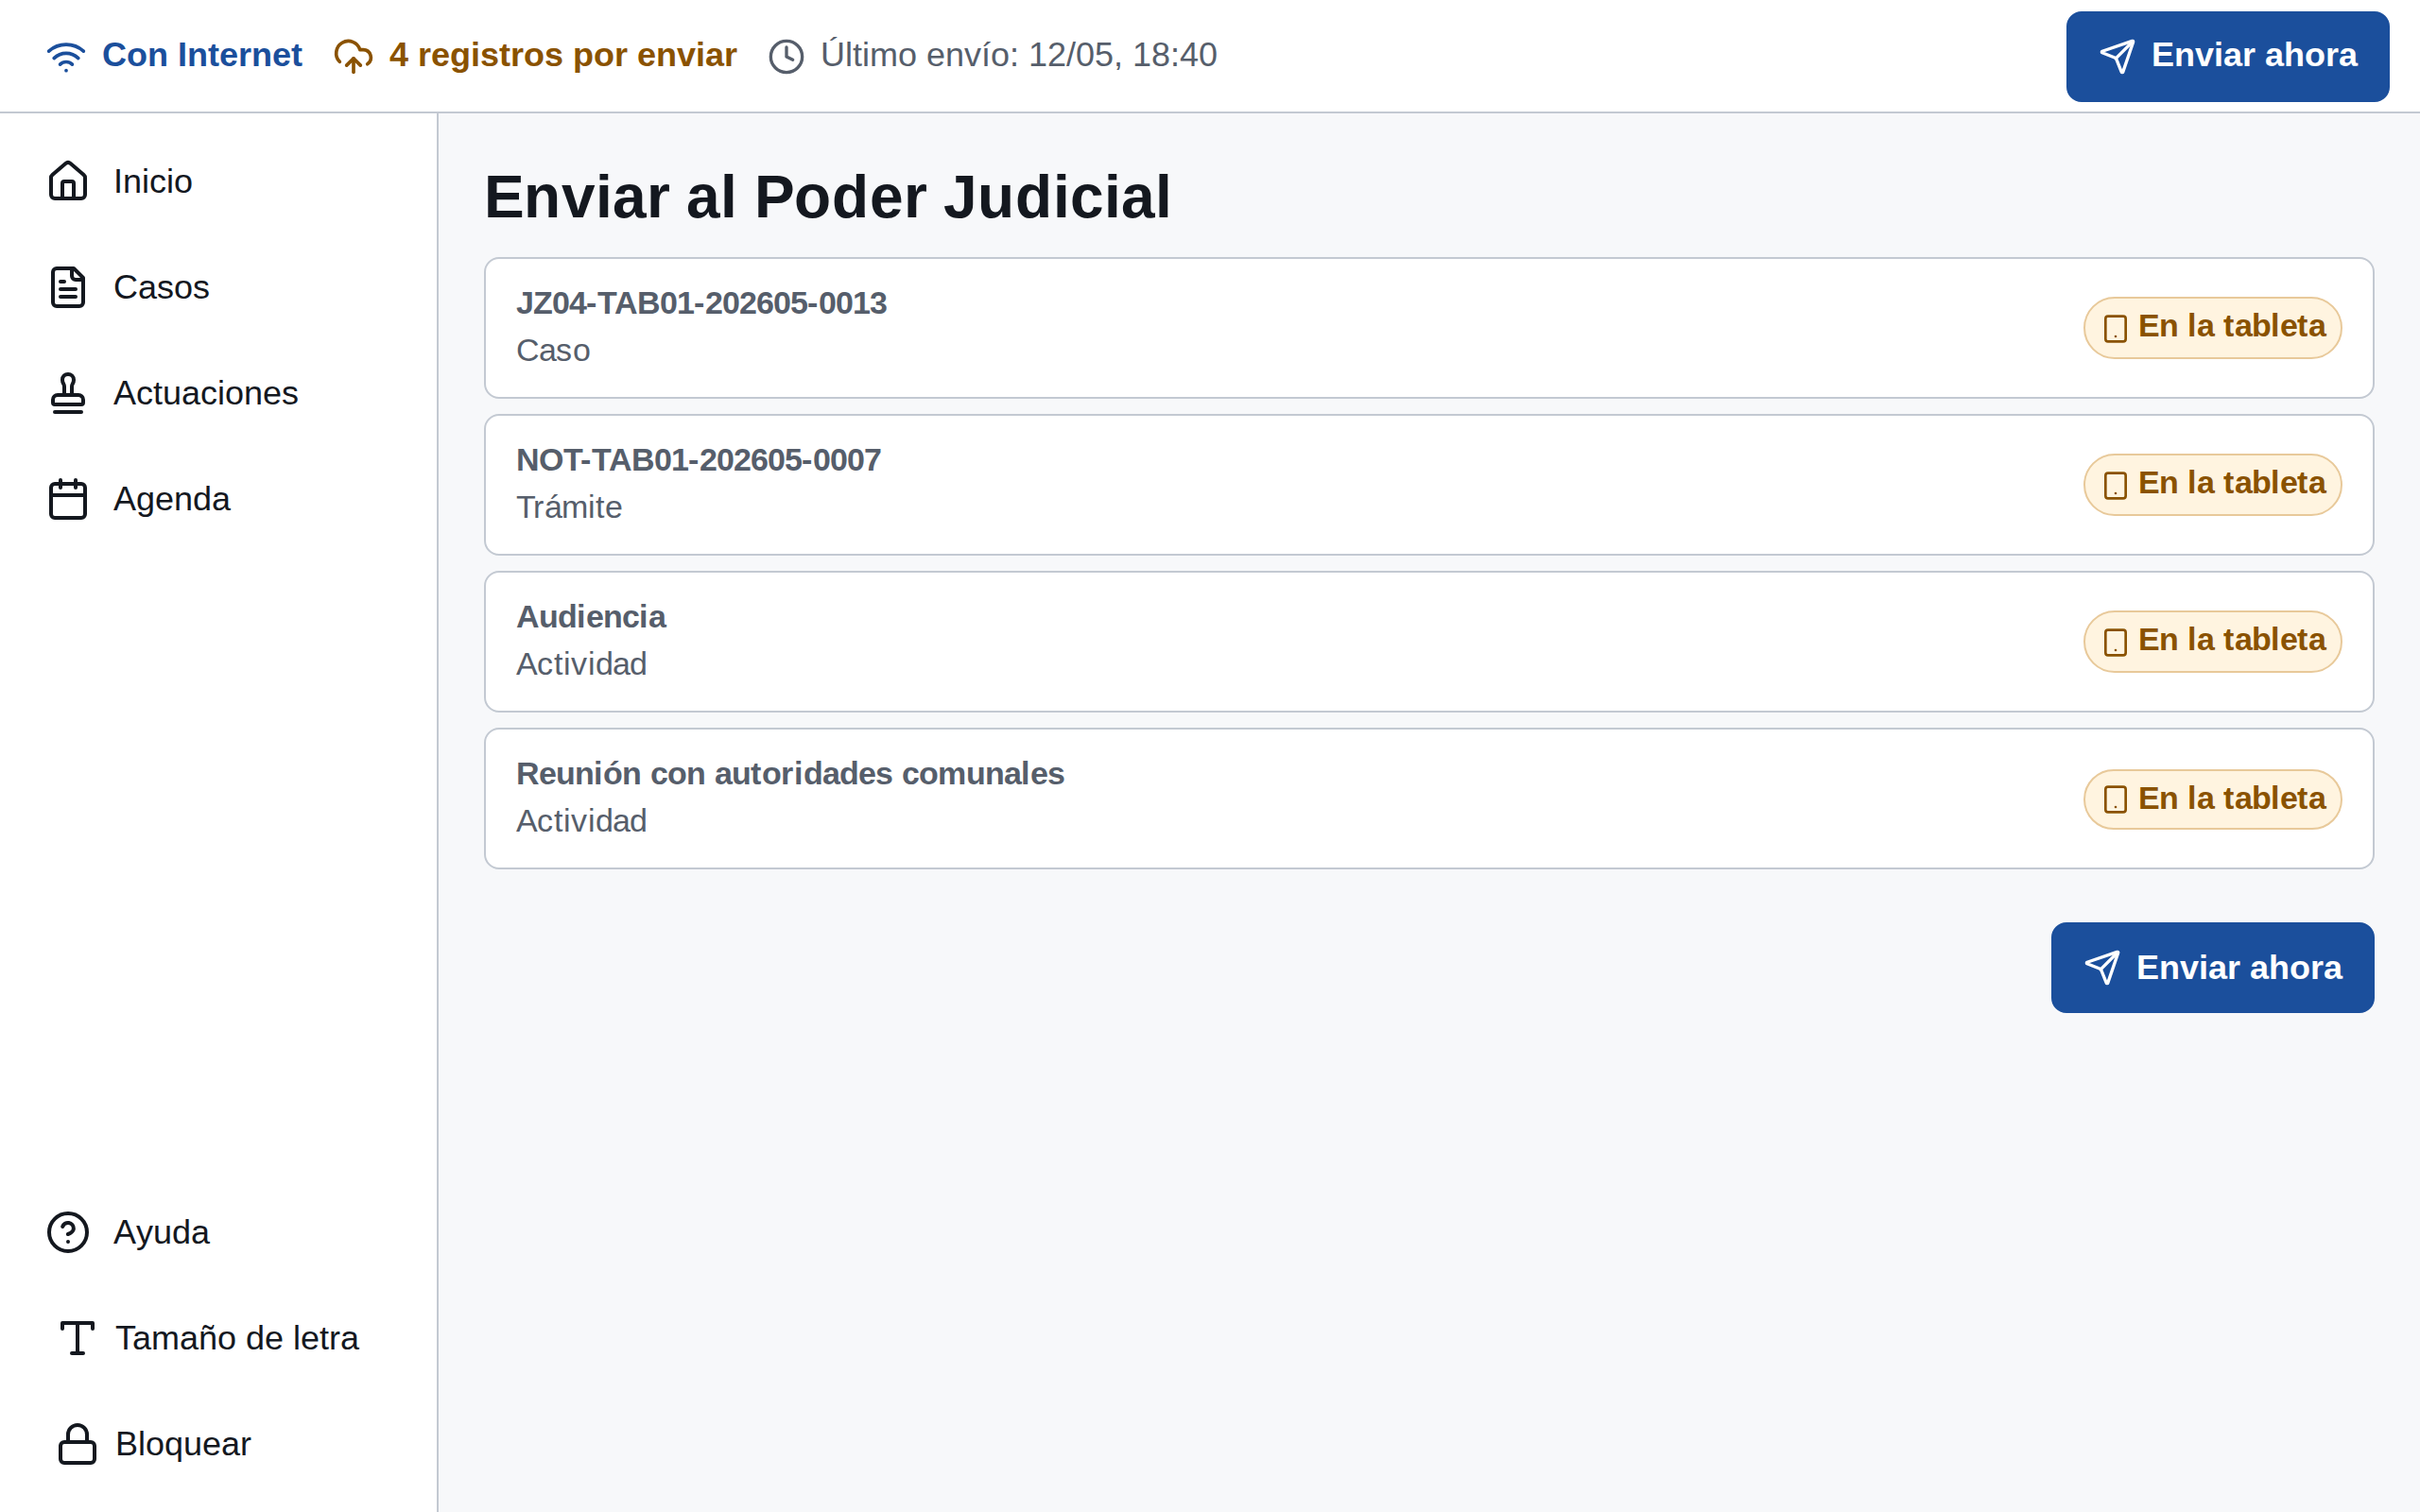
\includegraphics[width=0.82\linewidth]{capturas/F4-03_vuelve-internet.png}
\caption{P-09 · 4. Vuelve el Internet. Con Internet aparece el botón Enviar ahora en la barra y en la pantalla}
\end{figure}
\begin{figure}[H]\centering
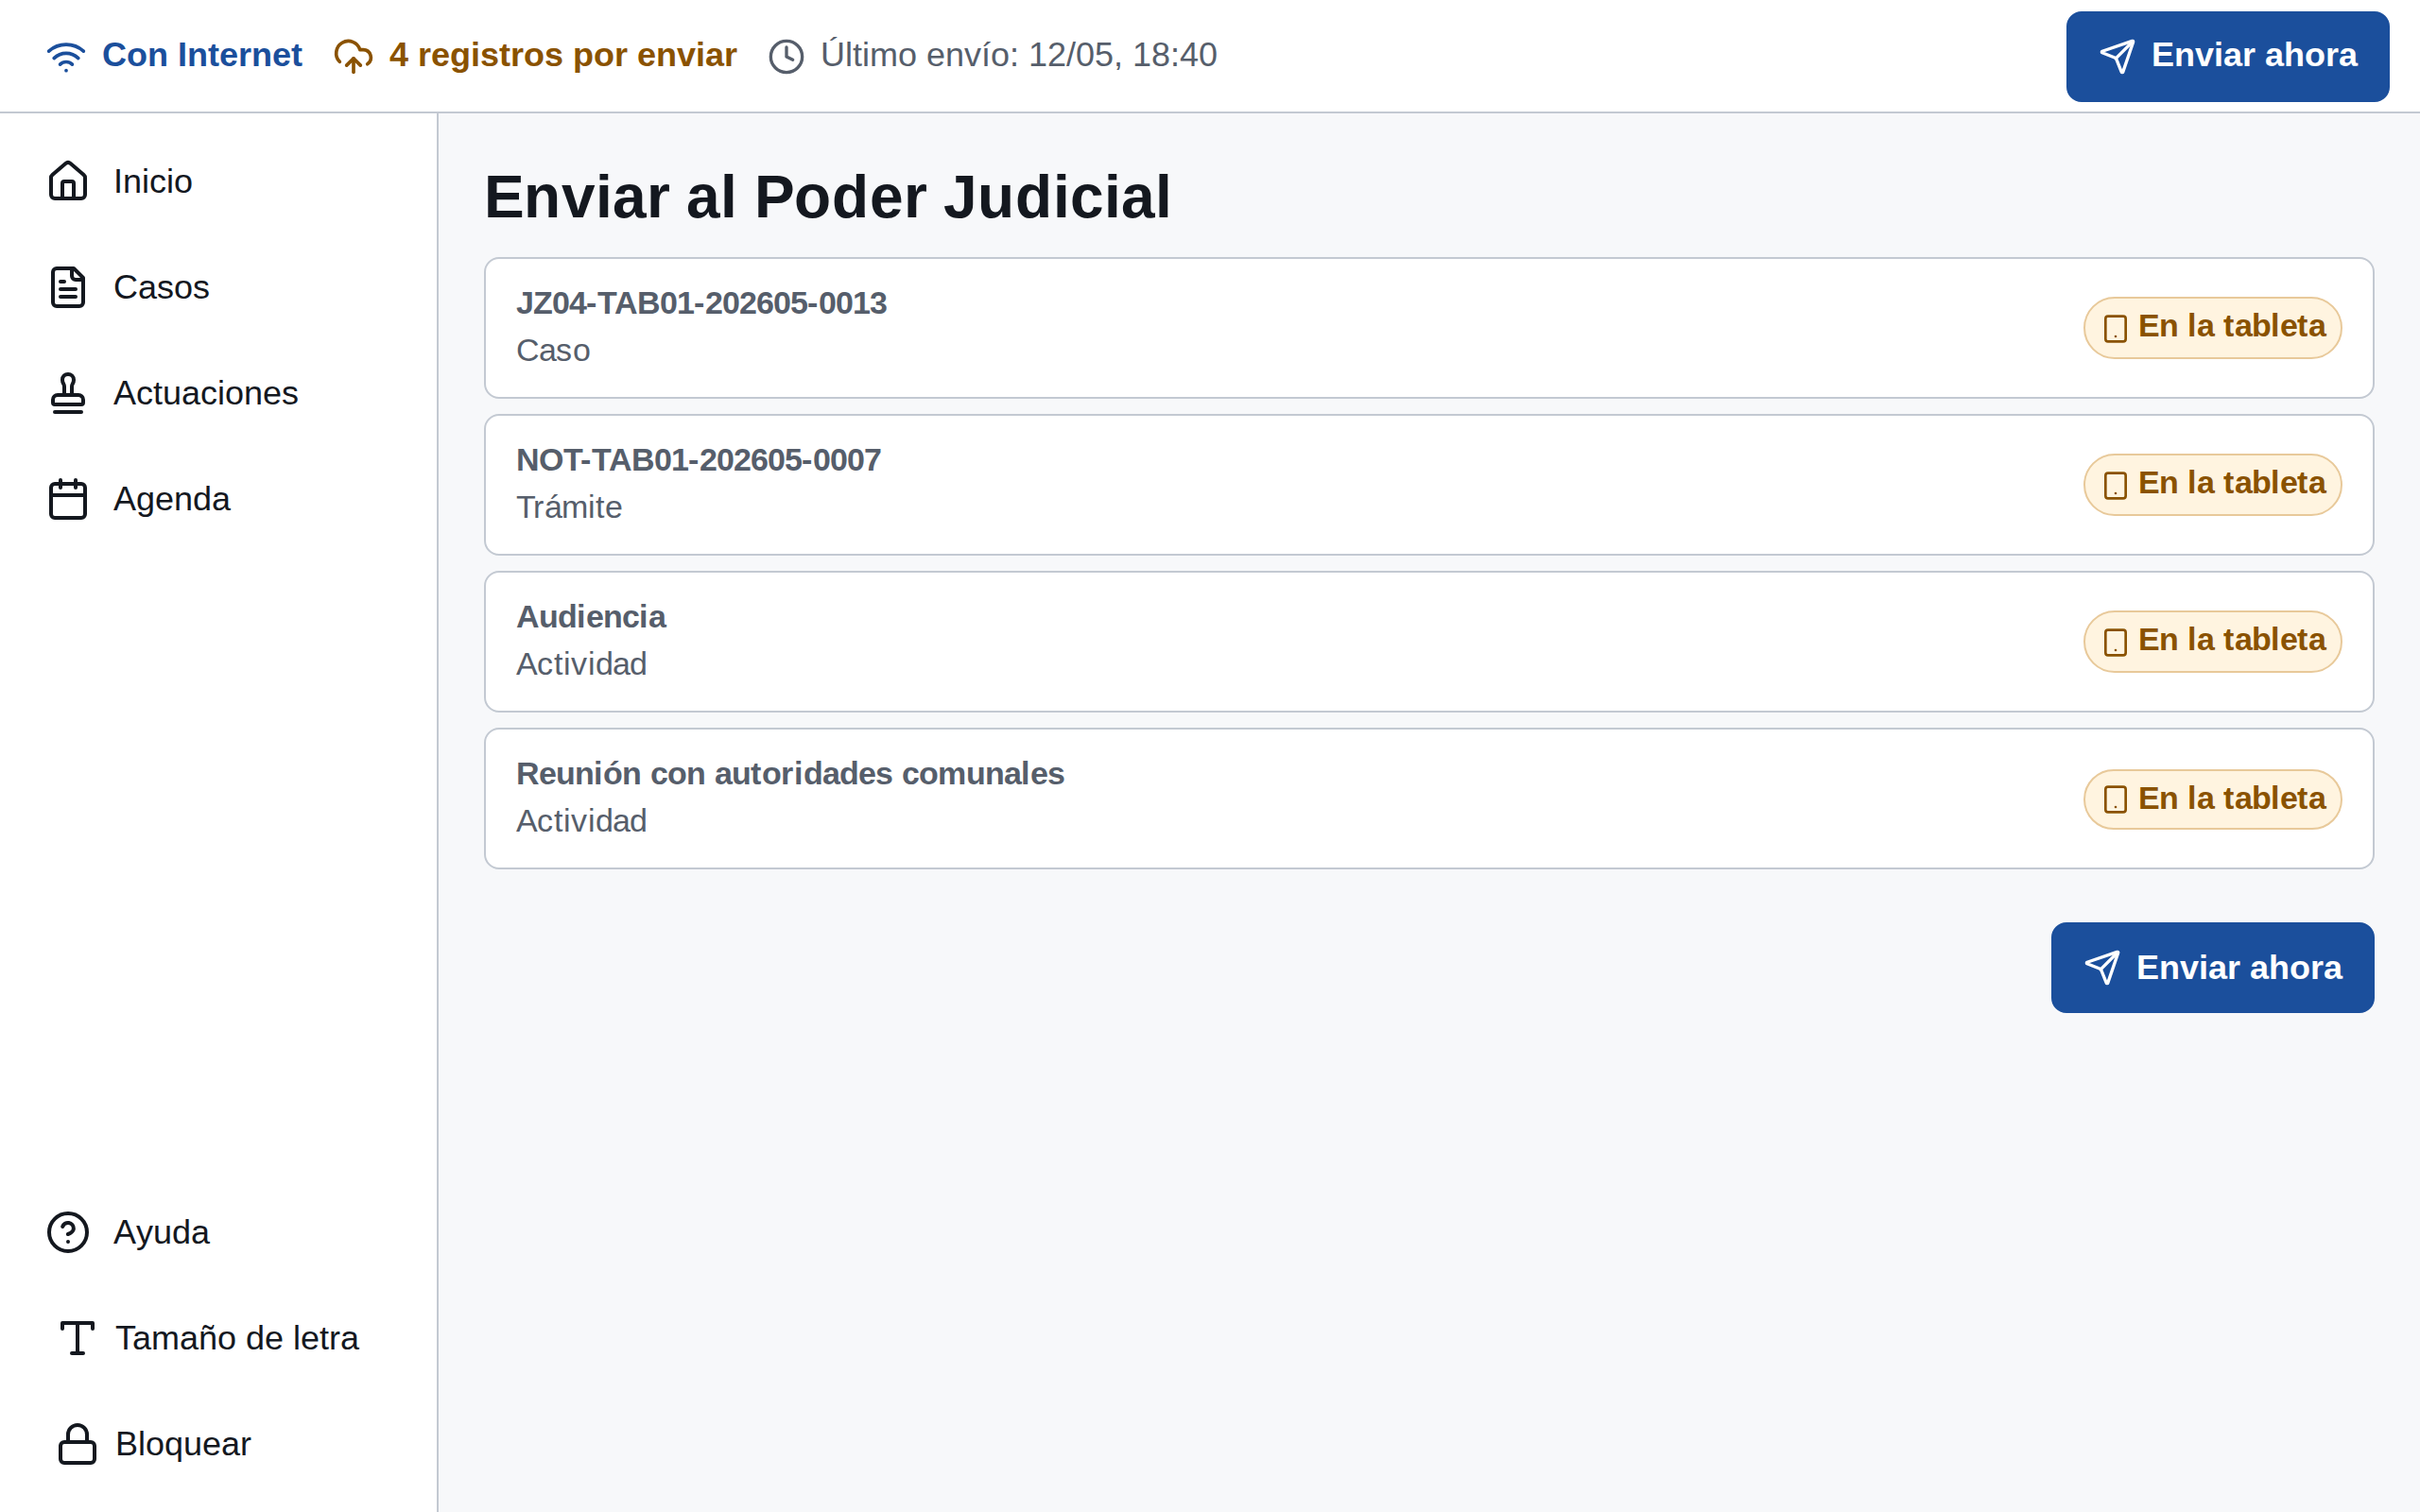
\includegraphics[width=0.82\linewidth]{capturas/F4-04_pendientes-del-dia.png}
\caption{P-09 · 5. Los cuatro registros del día. La pantalla de envío lista lo que la jueza registró en el día: el caso, su audiencia, el trámite y la reunión}
\end{figure}
\begin{figure}[H]\centering
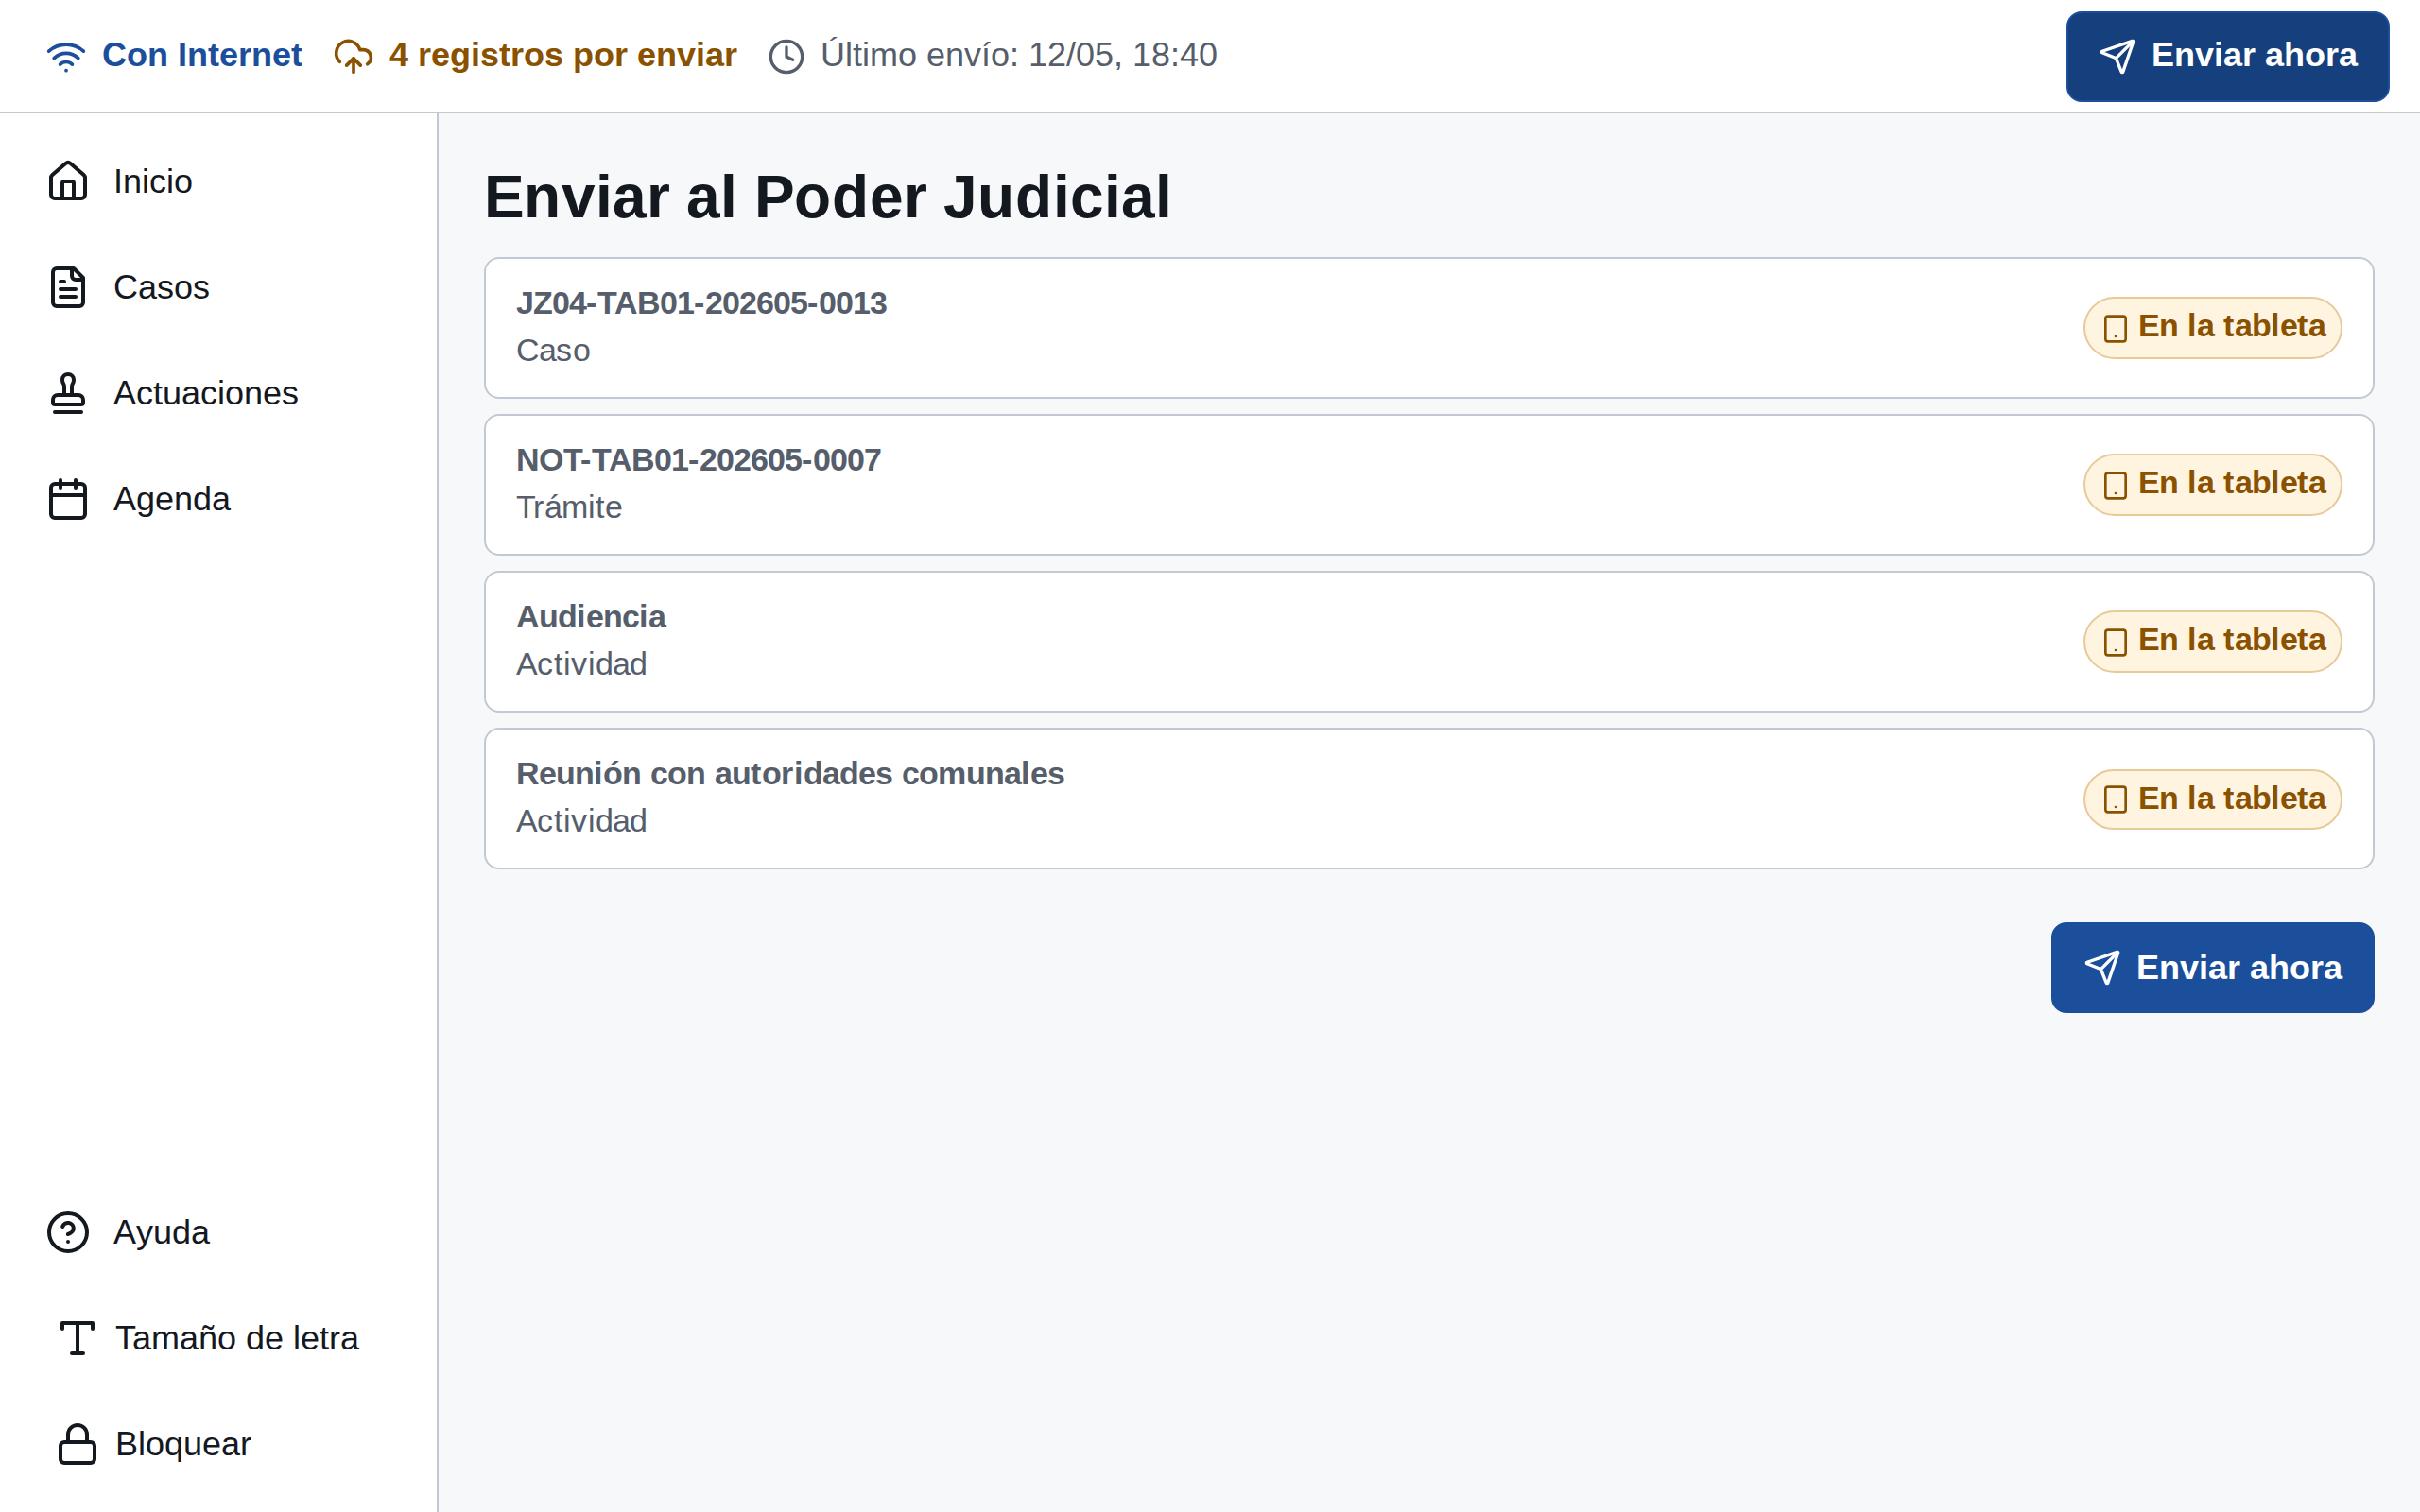
\includegraphics[width=0.82\linewidth]{capturas/F4-04b_progreso.png}
\caption{P-09 · 6. Enviando. Progreso del envío de los cuatro registros del día}
\end{figure}
\begin{figure}[H]\centering
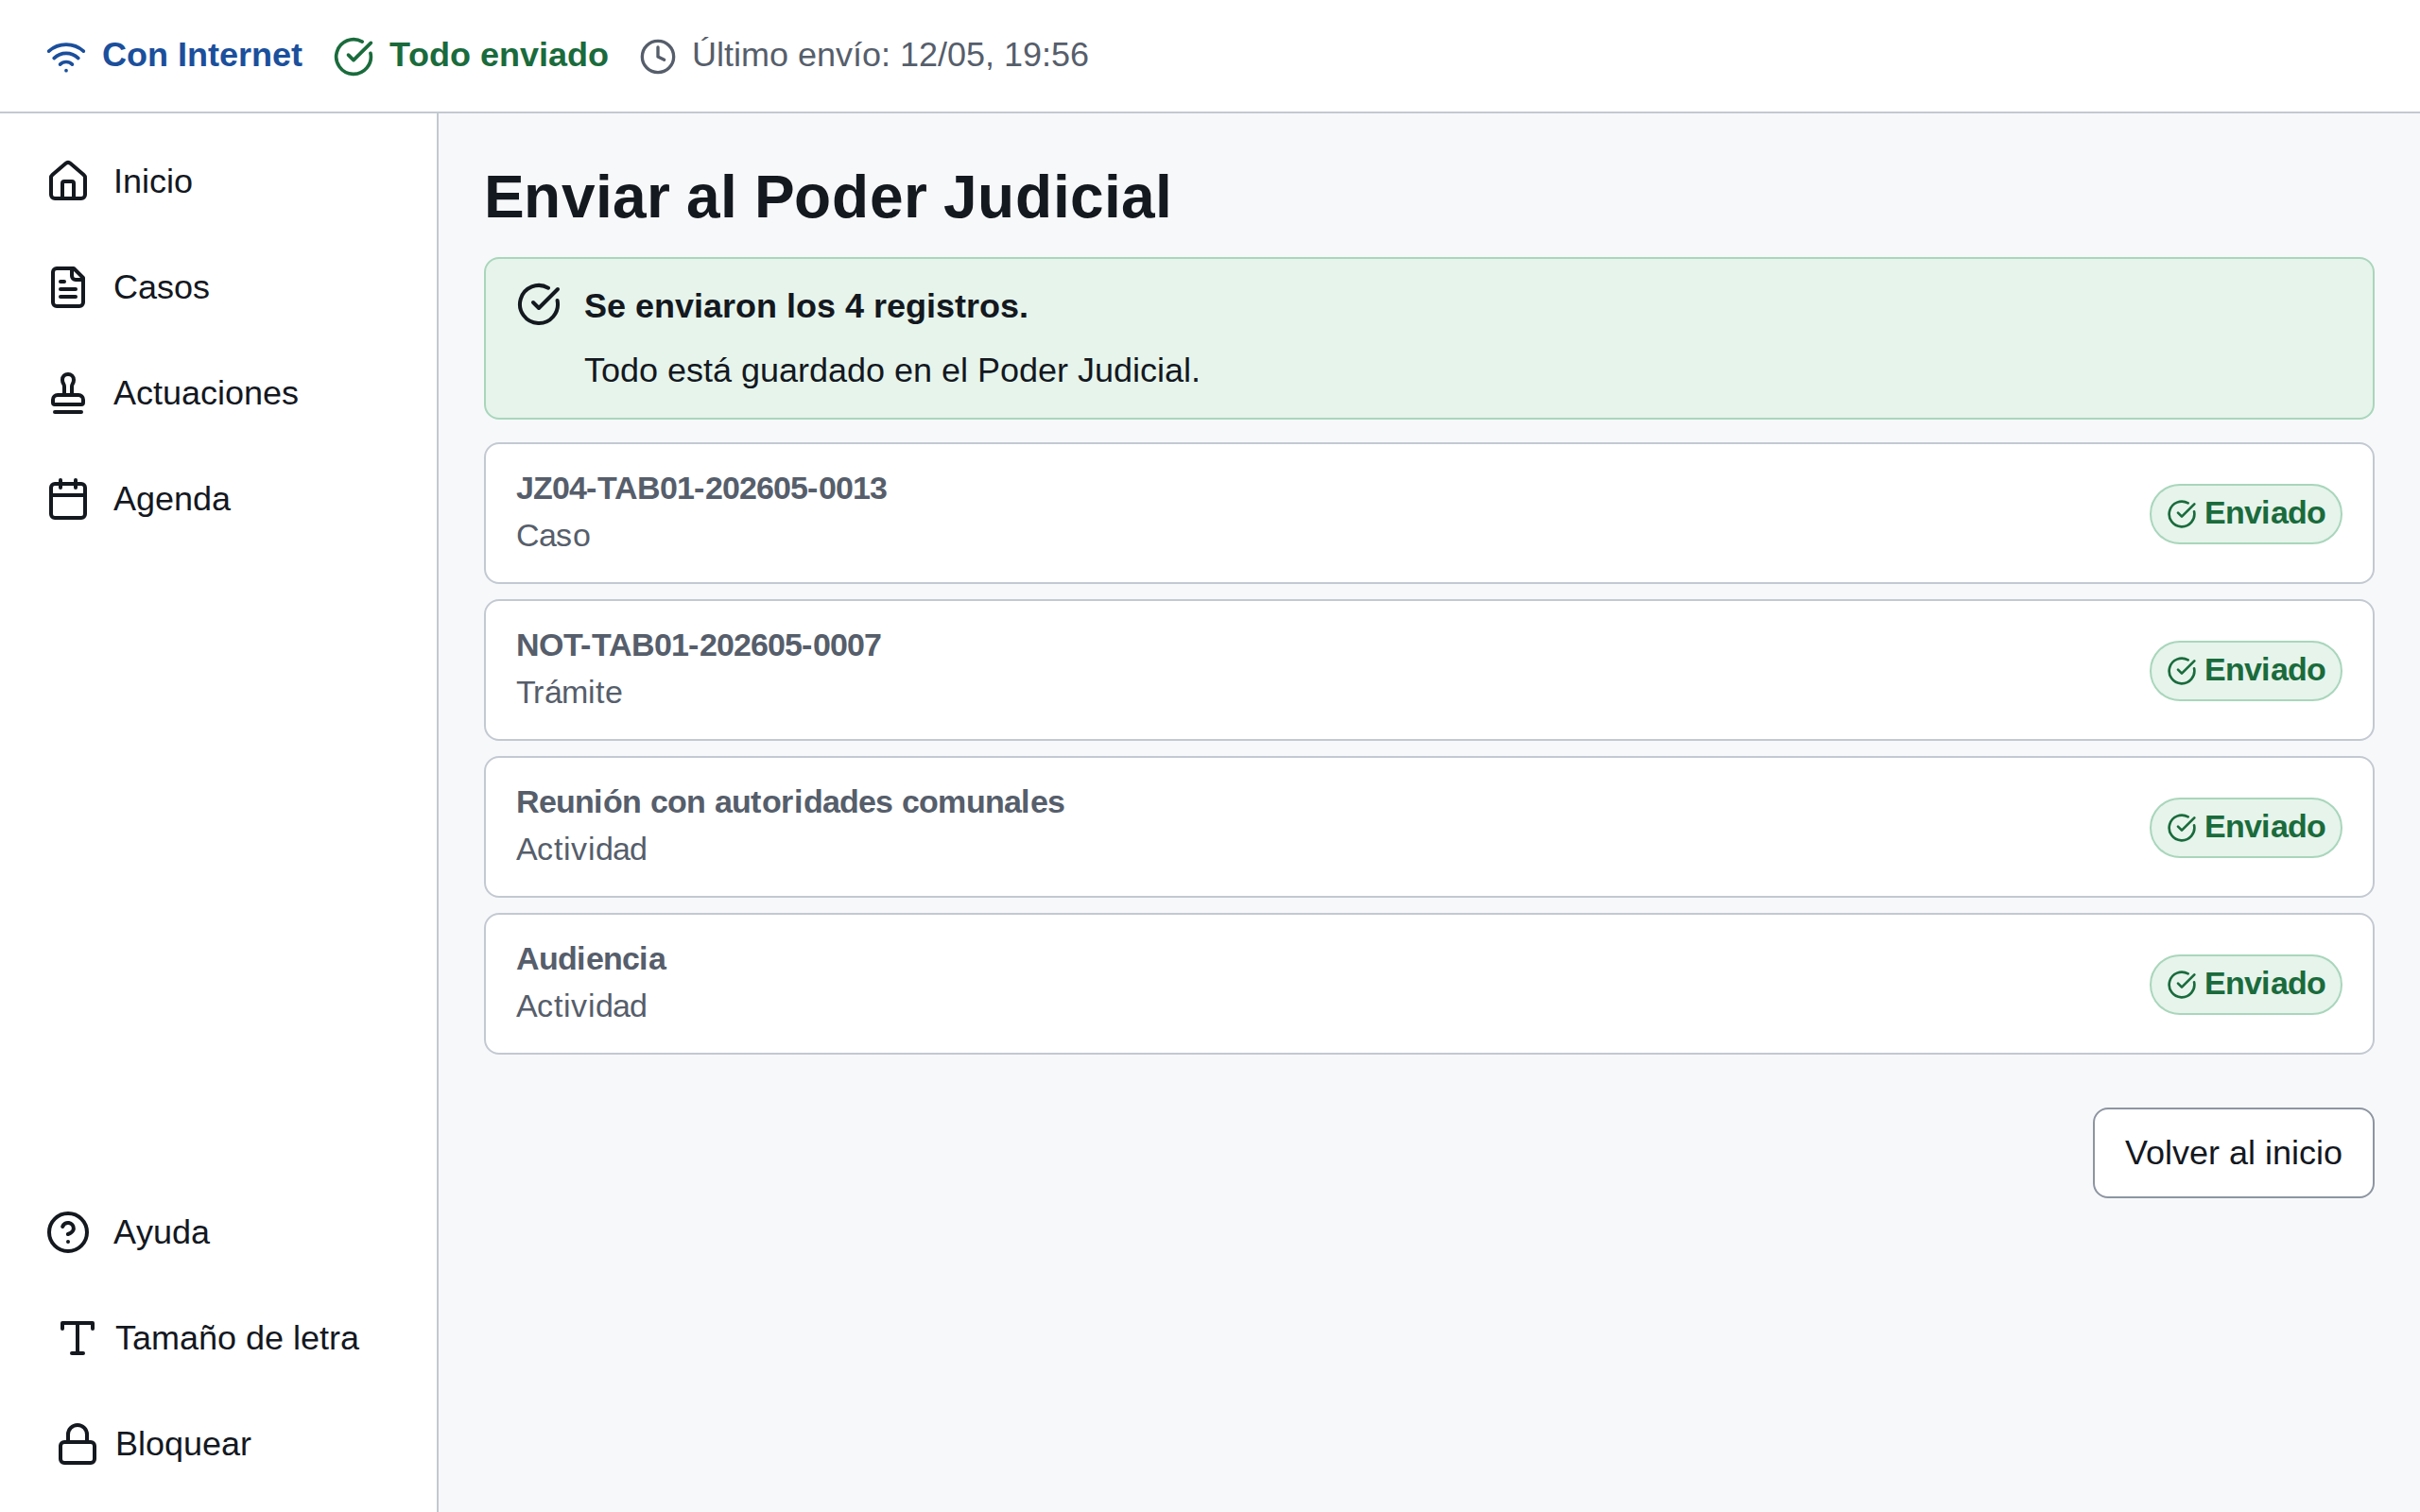
\includegraphics[width=0.82\linewidth]{capturas/F4-05_exito.png}
\caption{P-09 · 7. Envío completo. Se enviaron los 4 registros del día y la barra pasa a Todo enviado}
\end{figure}
\subsection{Flujo complementario A · Actualizar el avance de un caso}
\begin{figure}[H]\centering
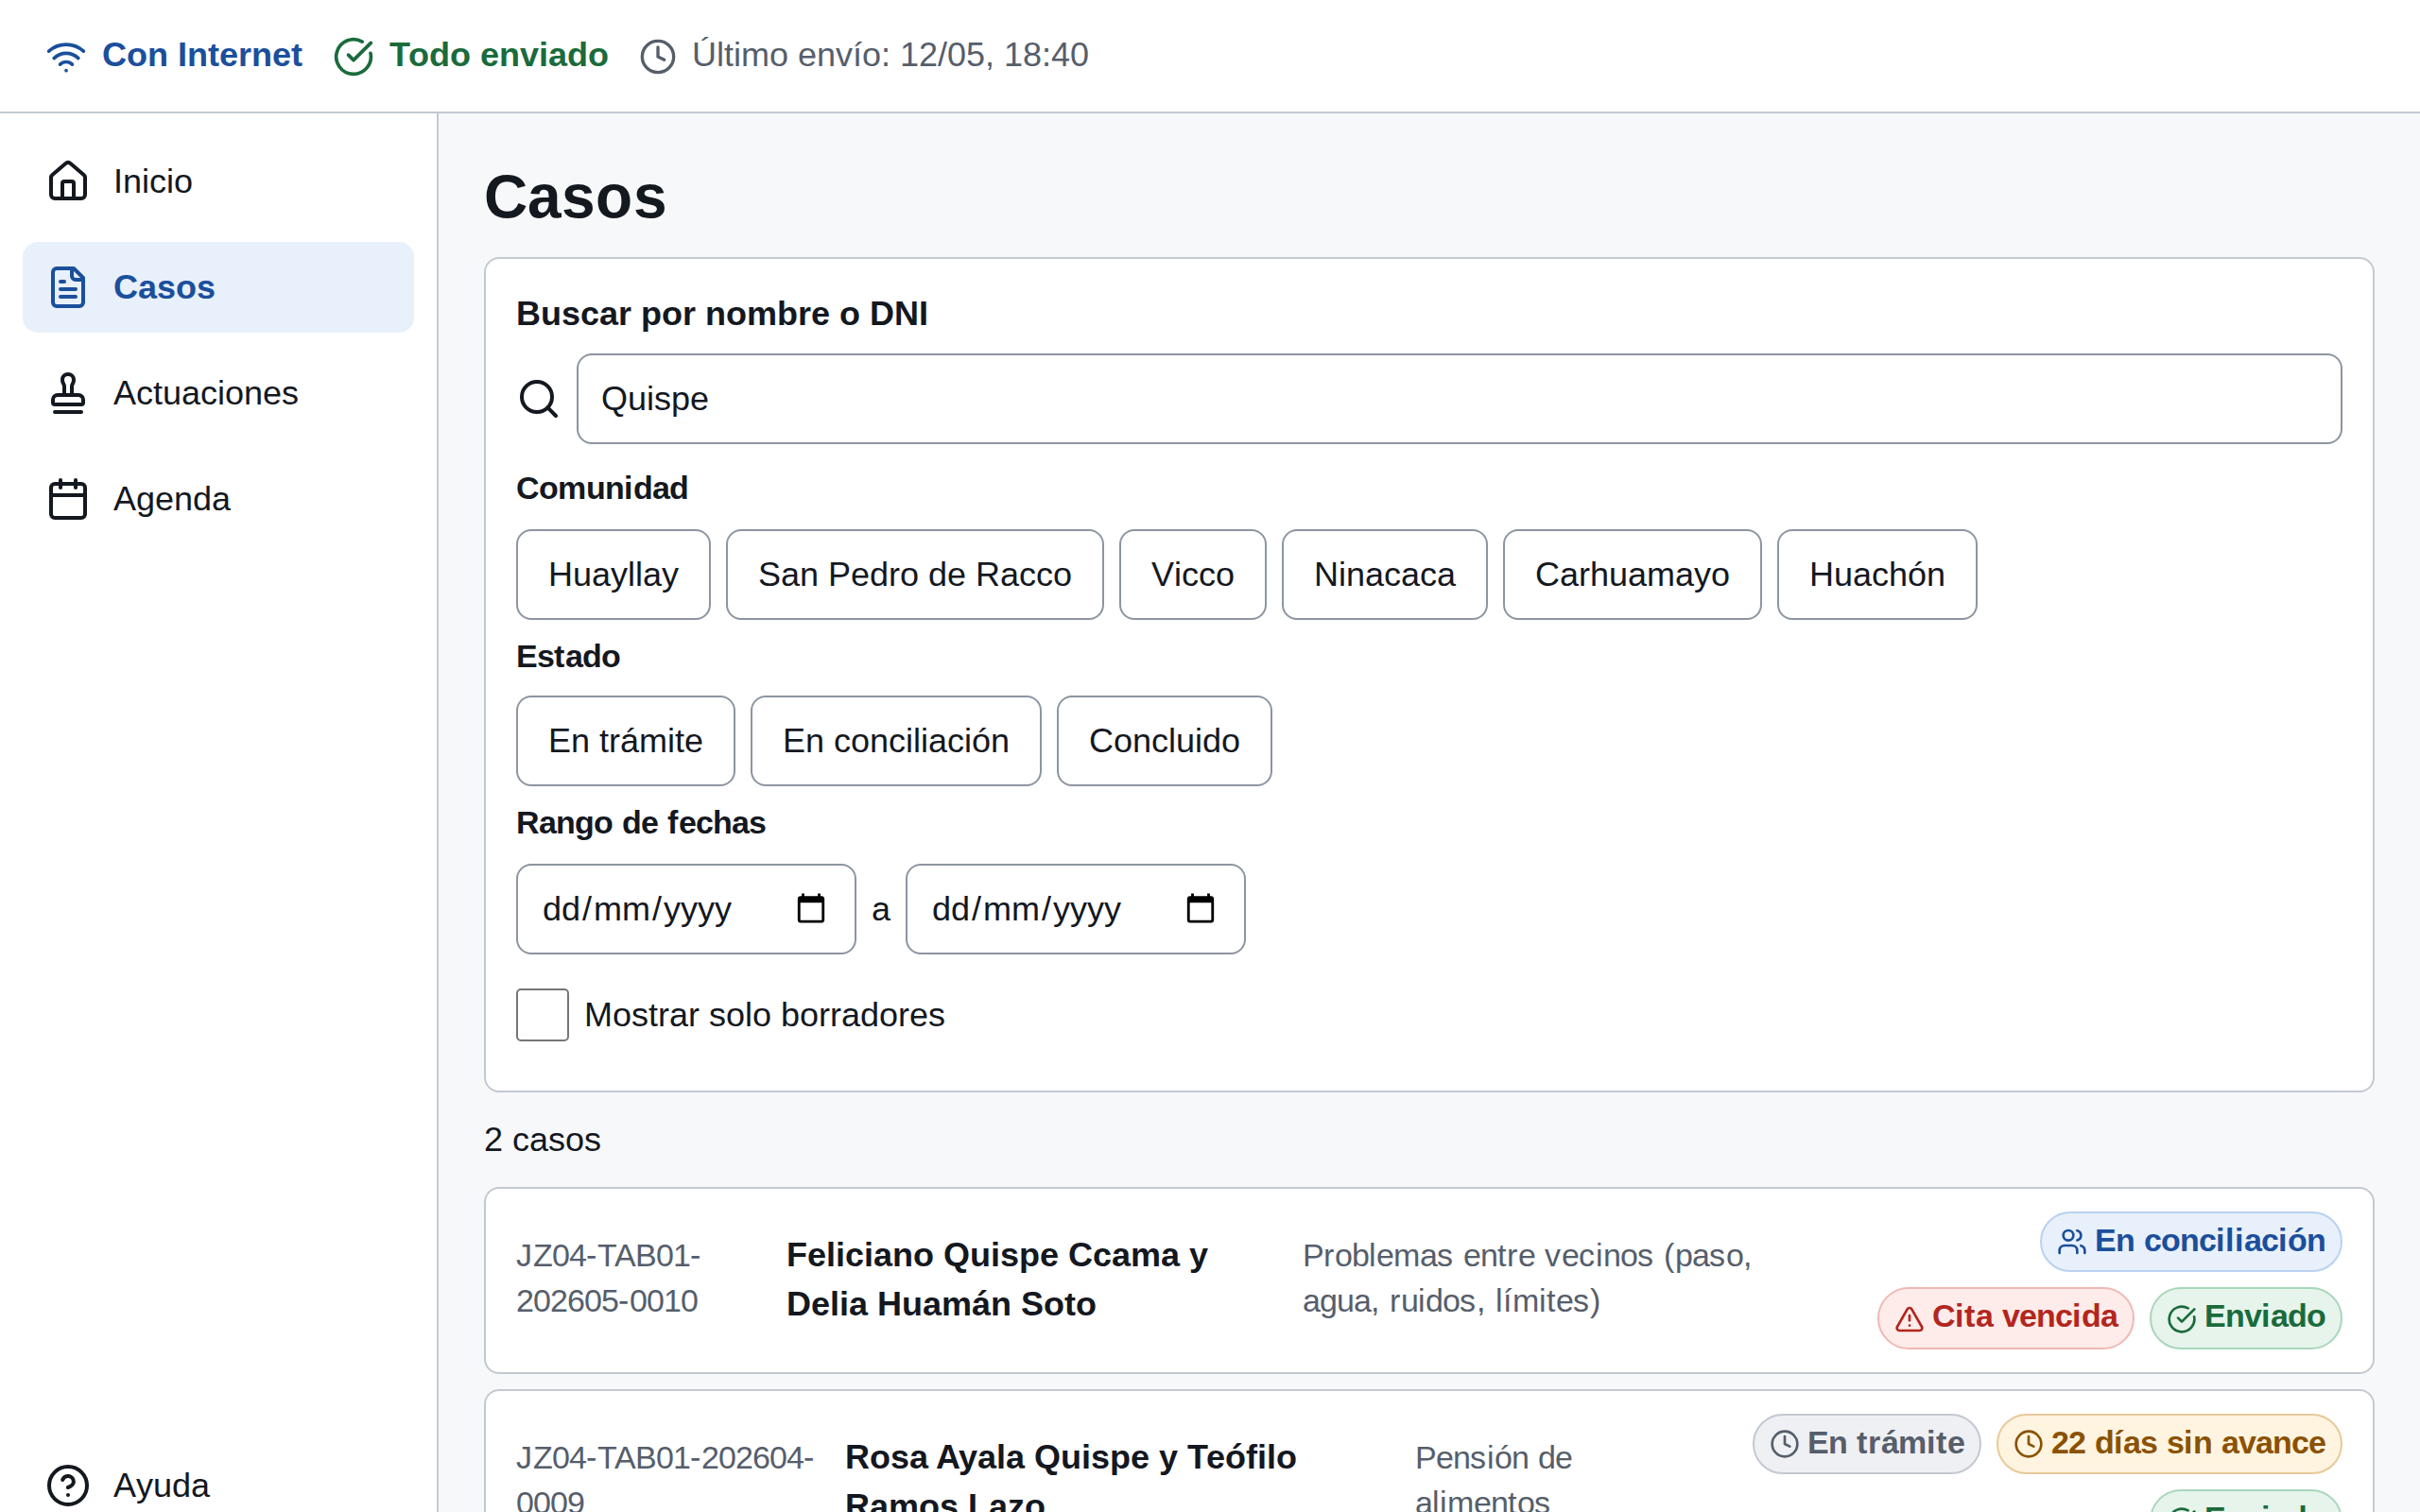
\includegraphics[width=0.82\linewidth]{capturas/FA-01_busqueda.png}
\caption{P-02 · 1. Búsqueda y filtros. Un solo campo busca por nombre o DNI; los filtros son botones visibles}
\end{figure}
\begin{figure}[H]\centering
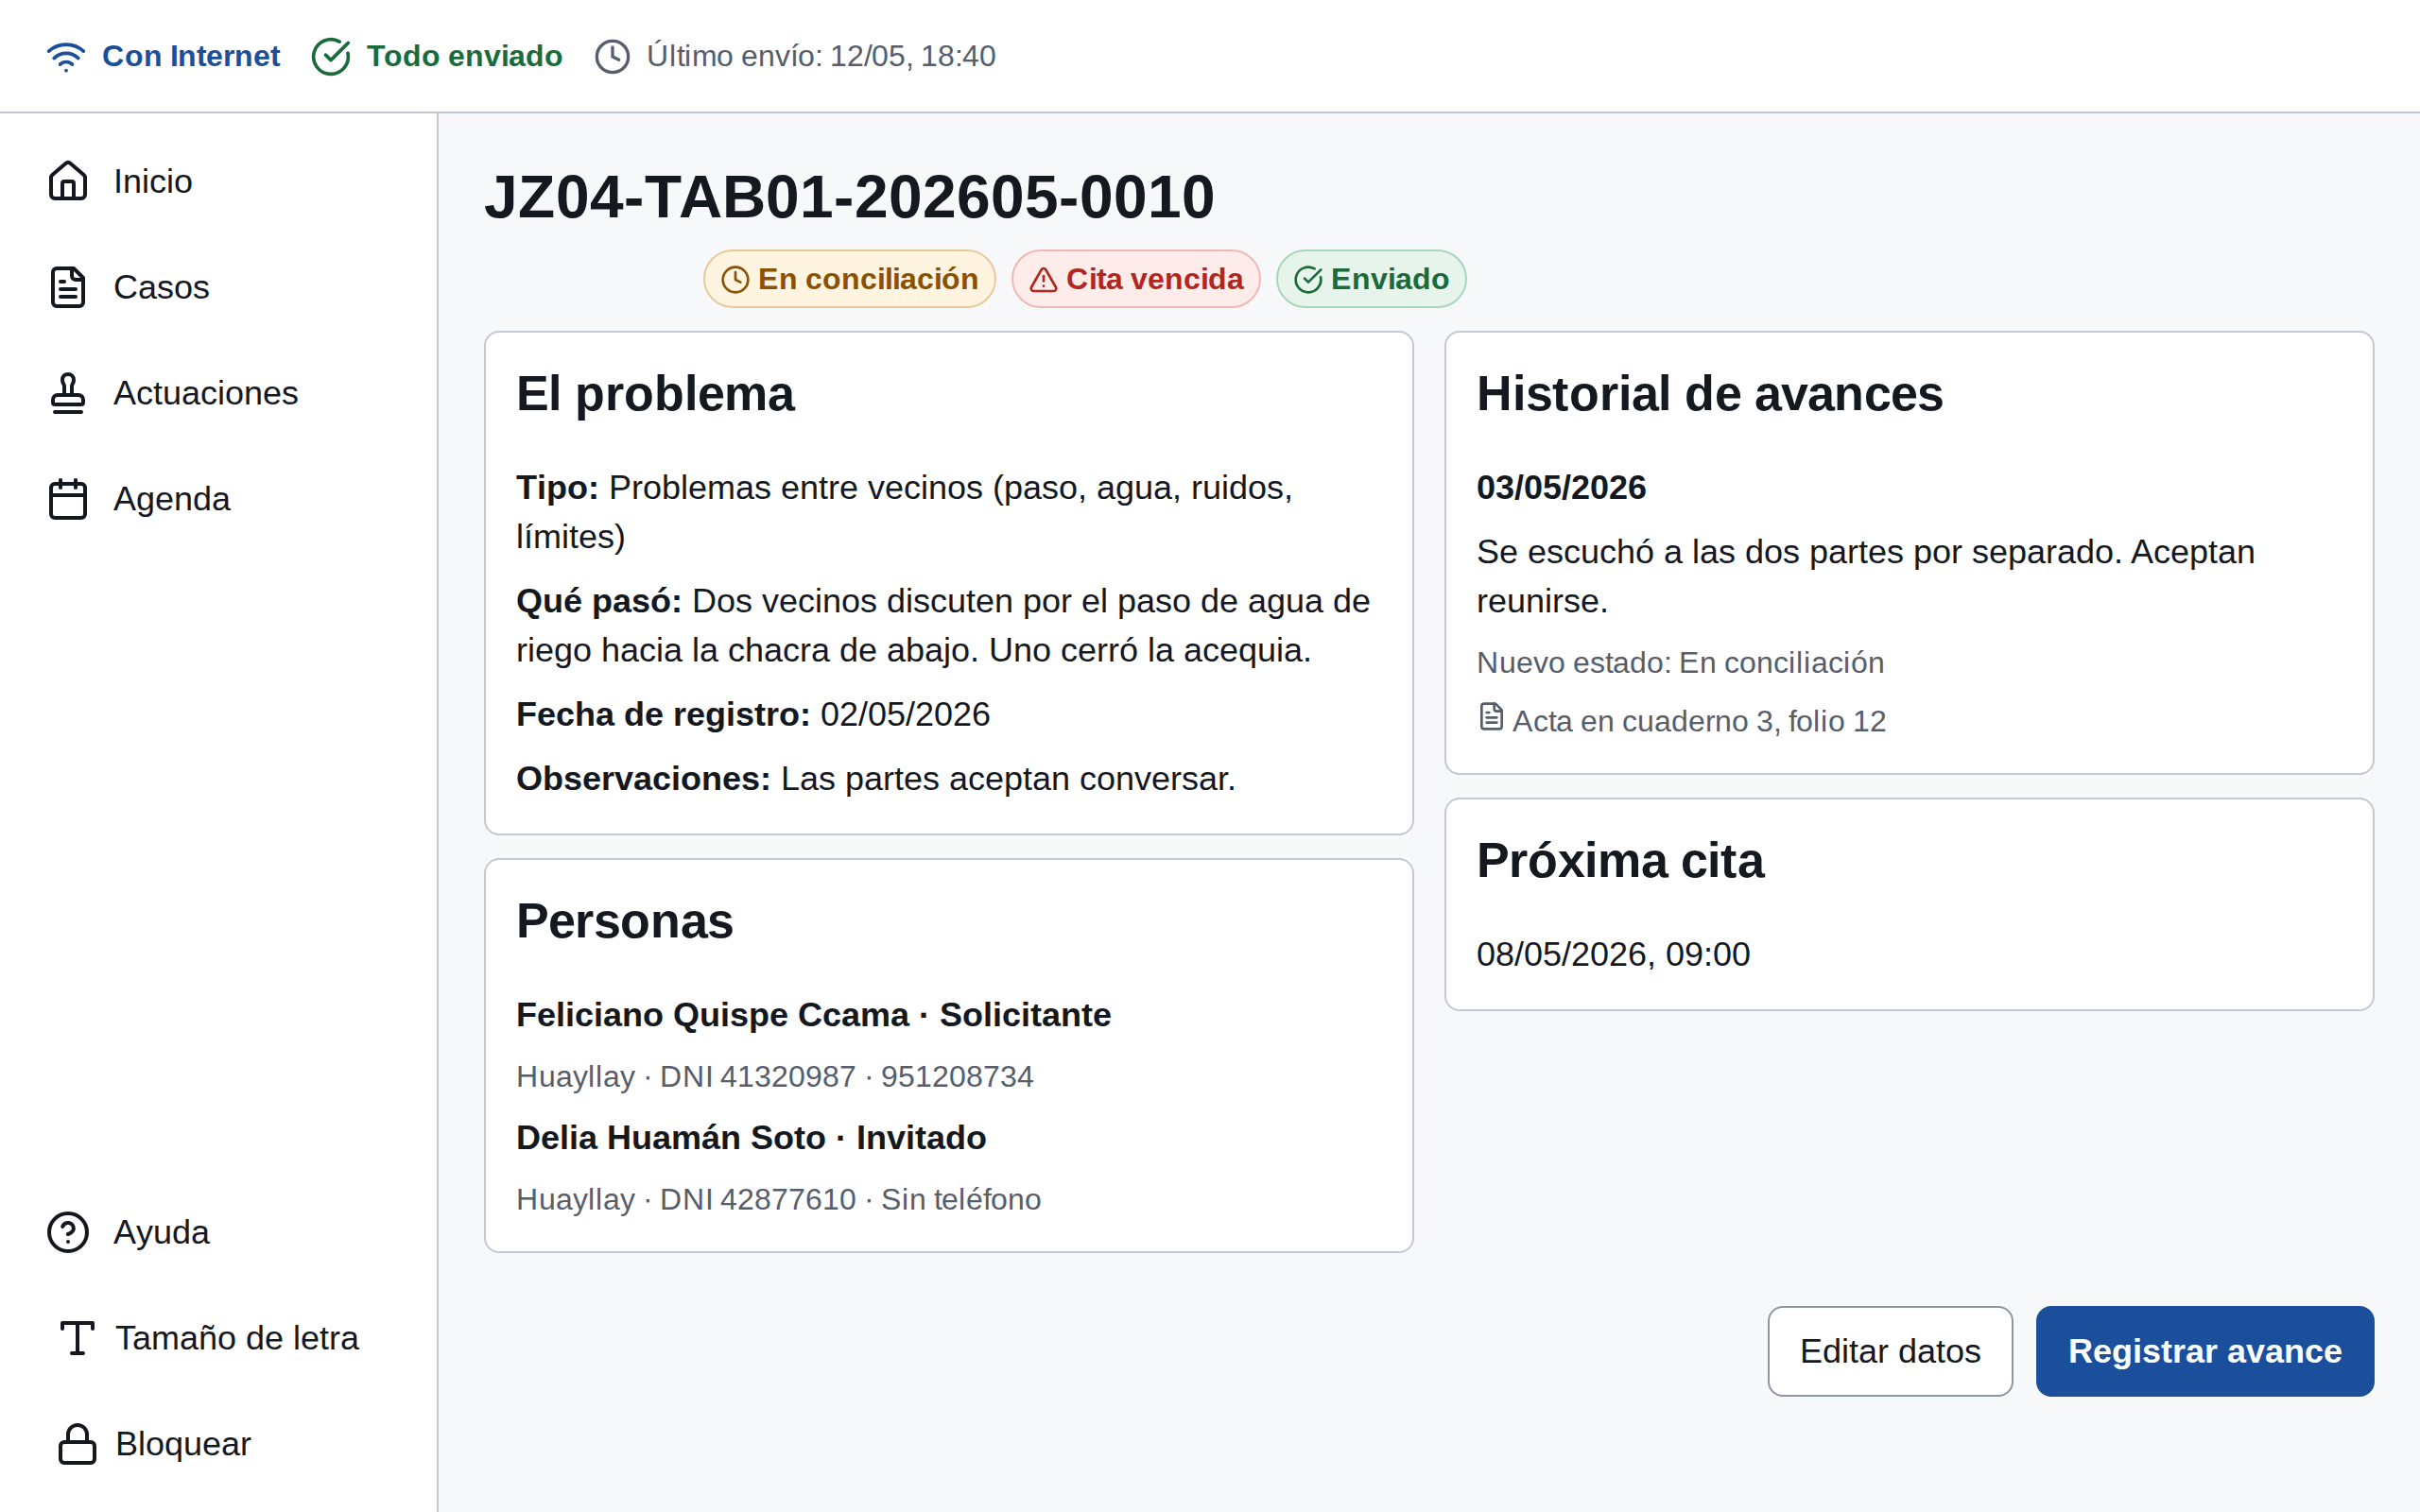
\includegraphics[width=0.82\linewidth]{capturas/FA-02_detalle-cita-vencida.png}
\caption{P-04 · 2. Caso con cita vencida. El motivo de atención se explica en texto, no solo con color}
\end{figure}
\begin{figure}[H]\centering
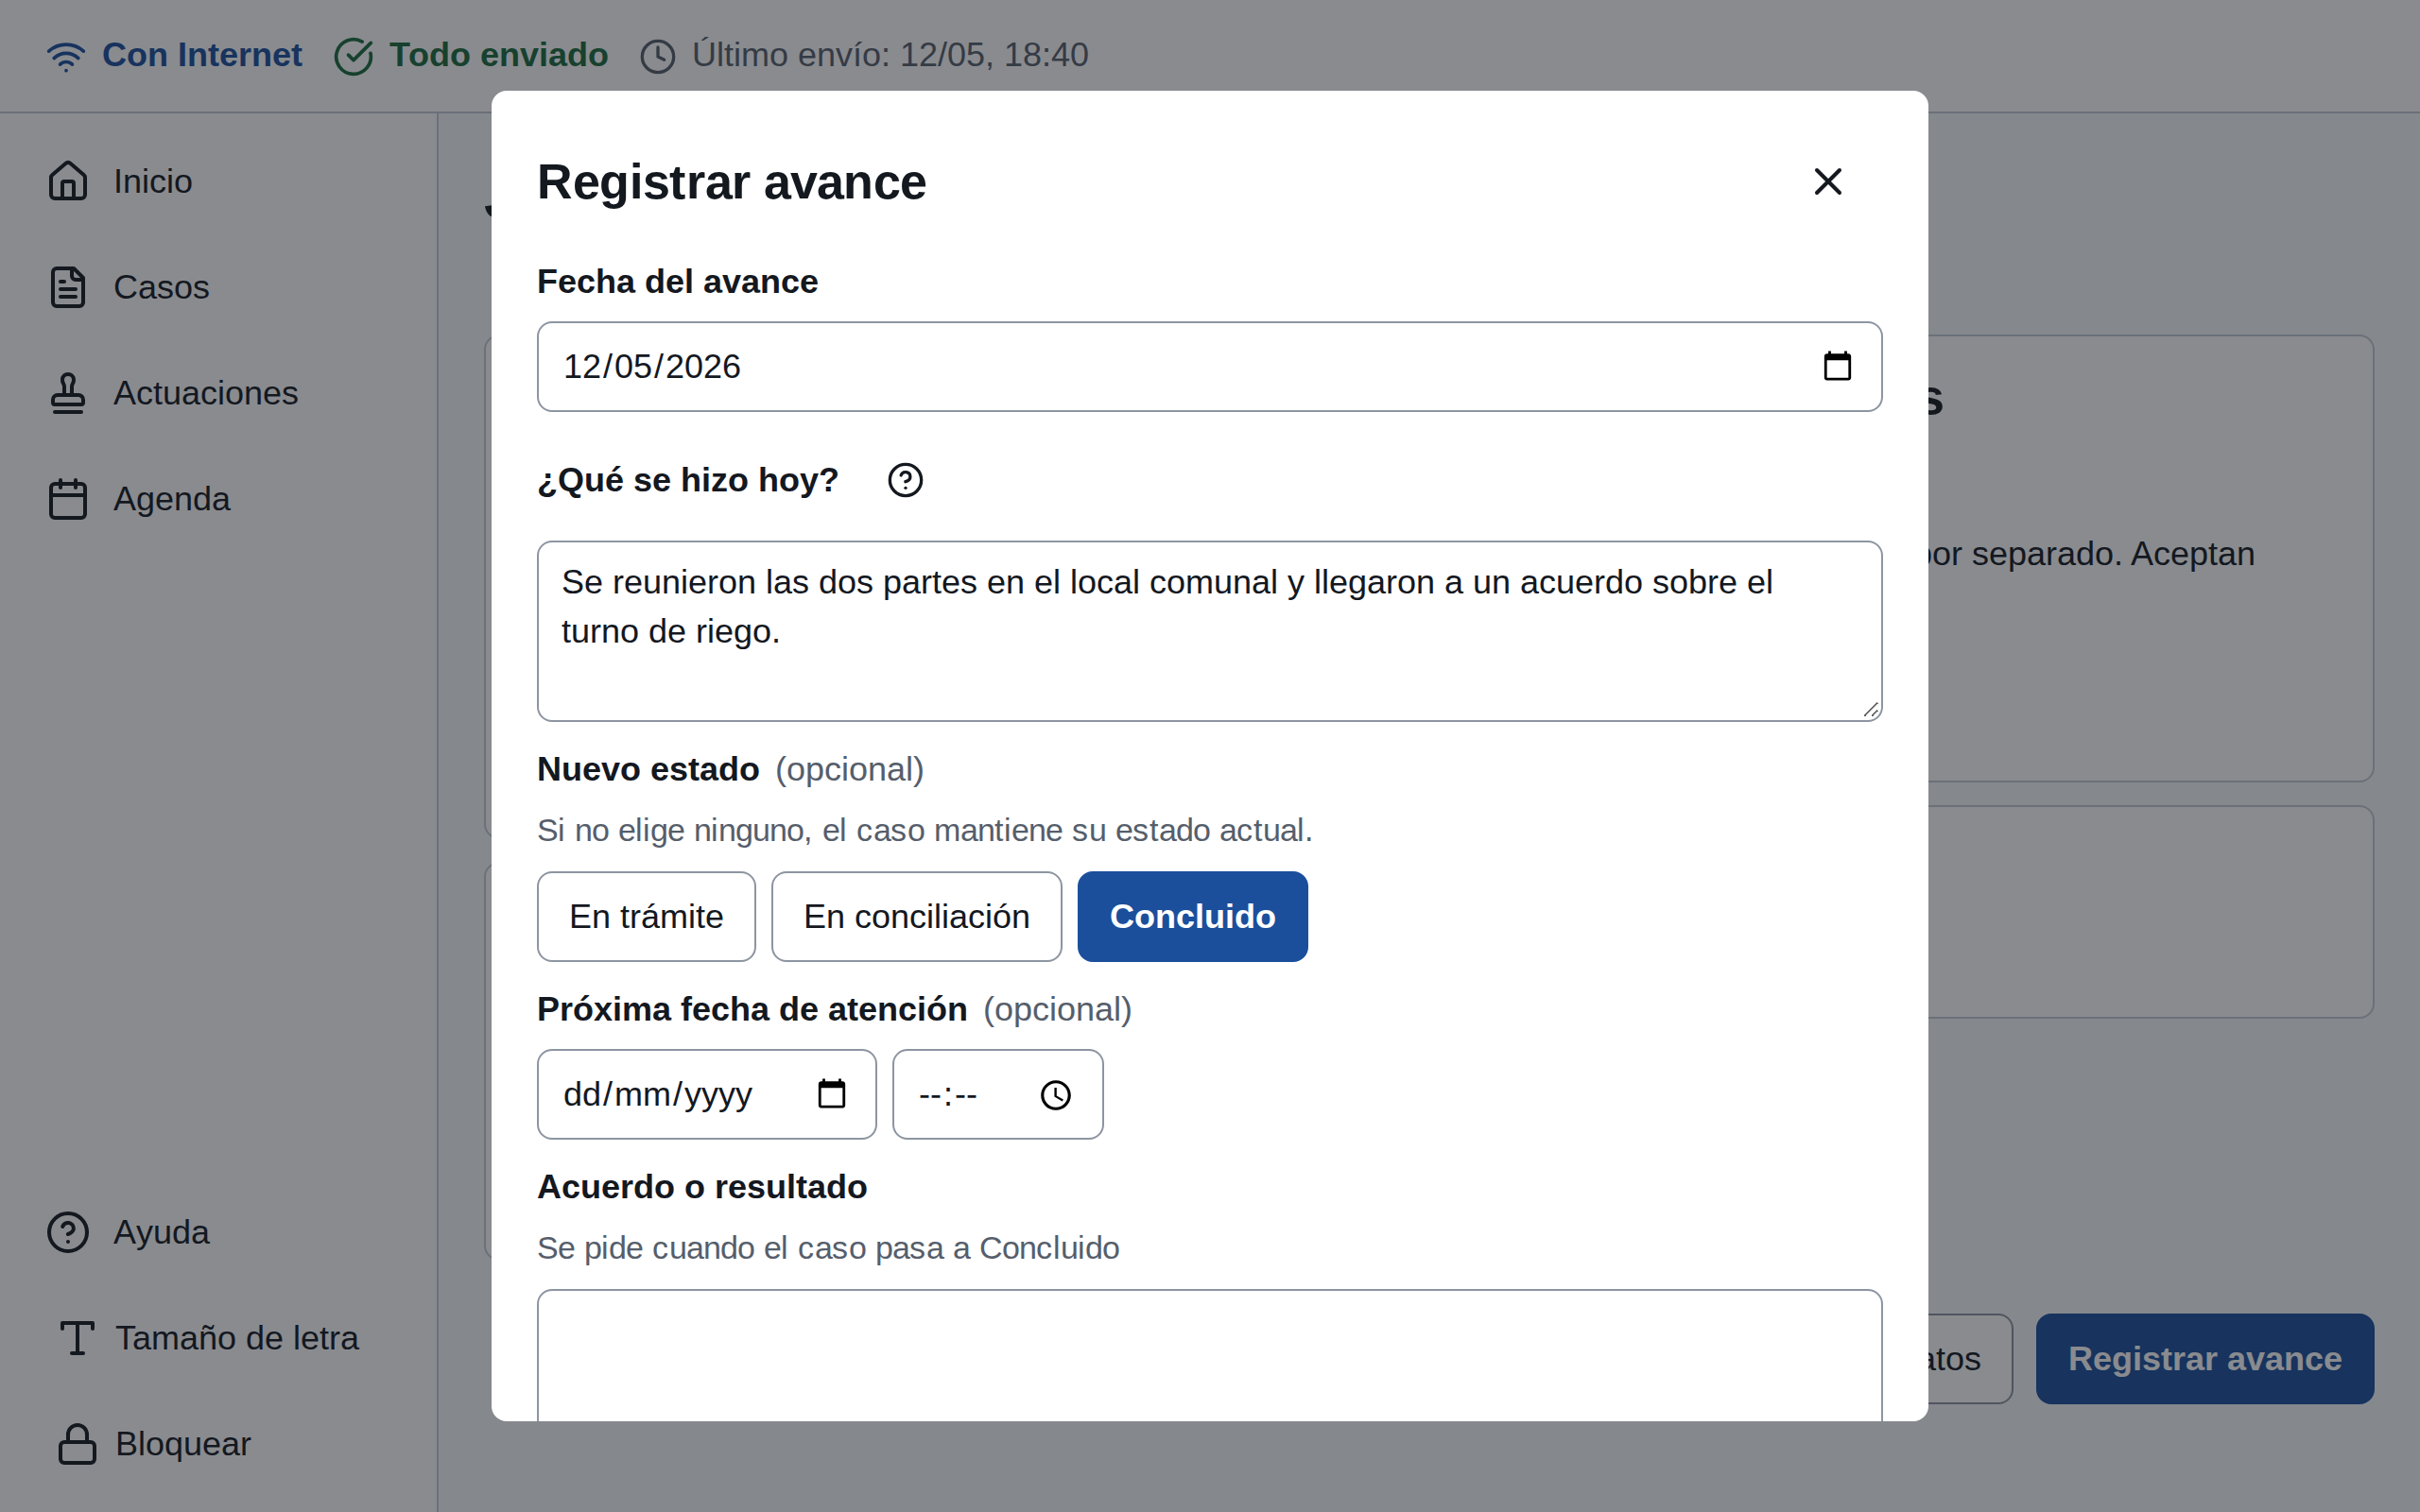
\includegraphics[width=0.82\linewidth]{capturas/FA-03_avance-condicional.png}
\caption{P-04 · 3. Al concluir se pide el acuerdo. El campo condicional aparece con su línea explicativa al pasar a Concluido}
\end{figure}
\begin{figure}[H]\centering
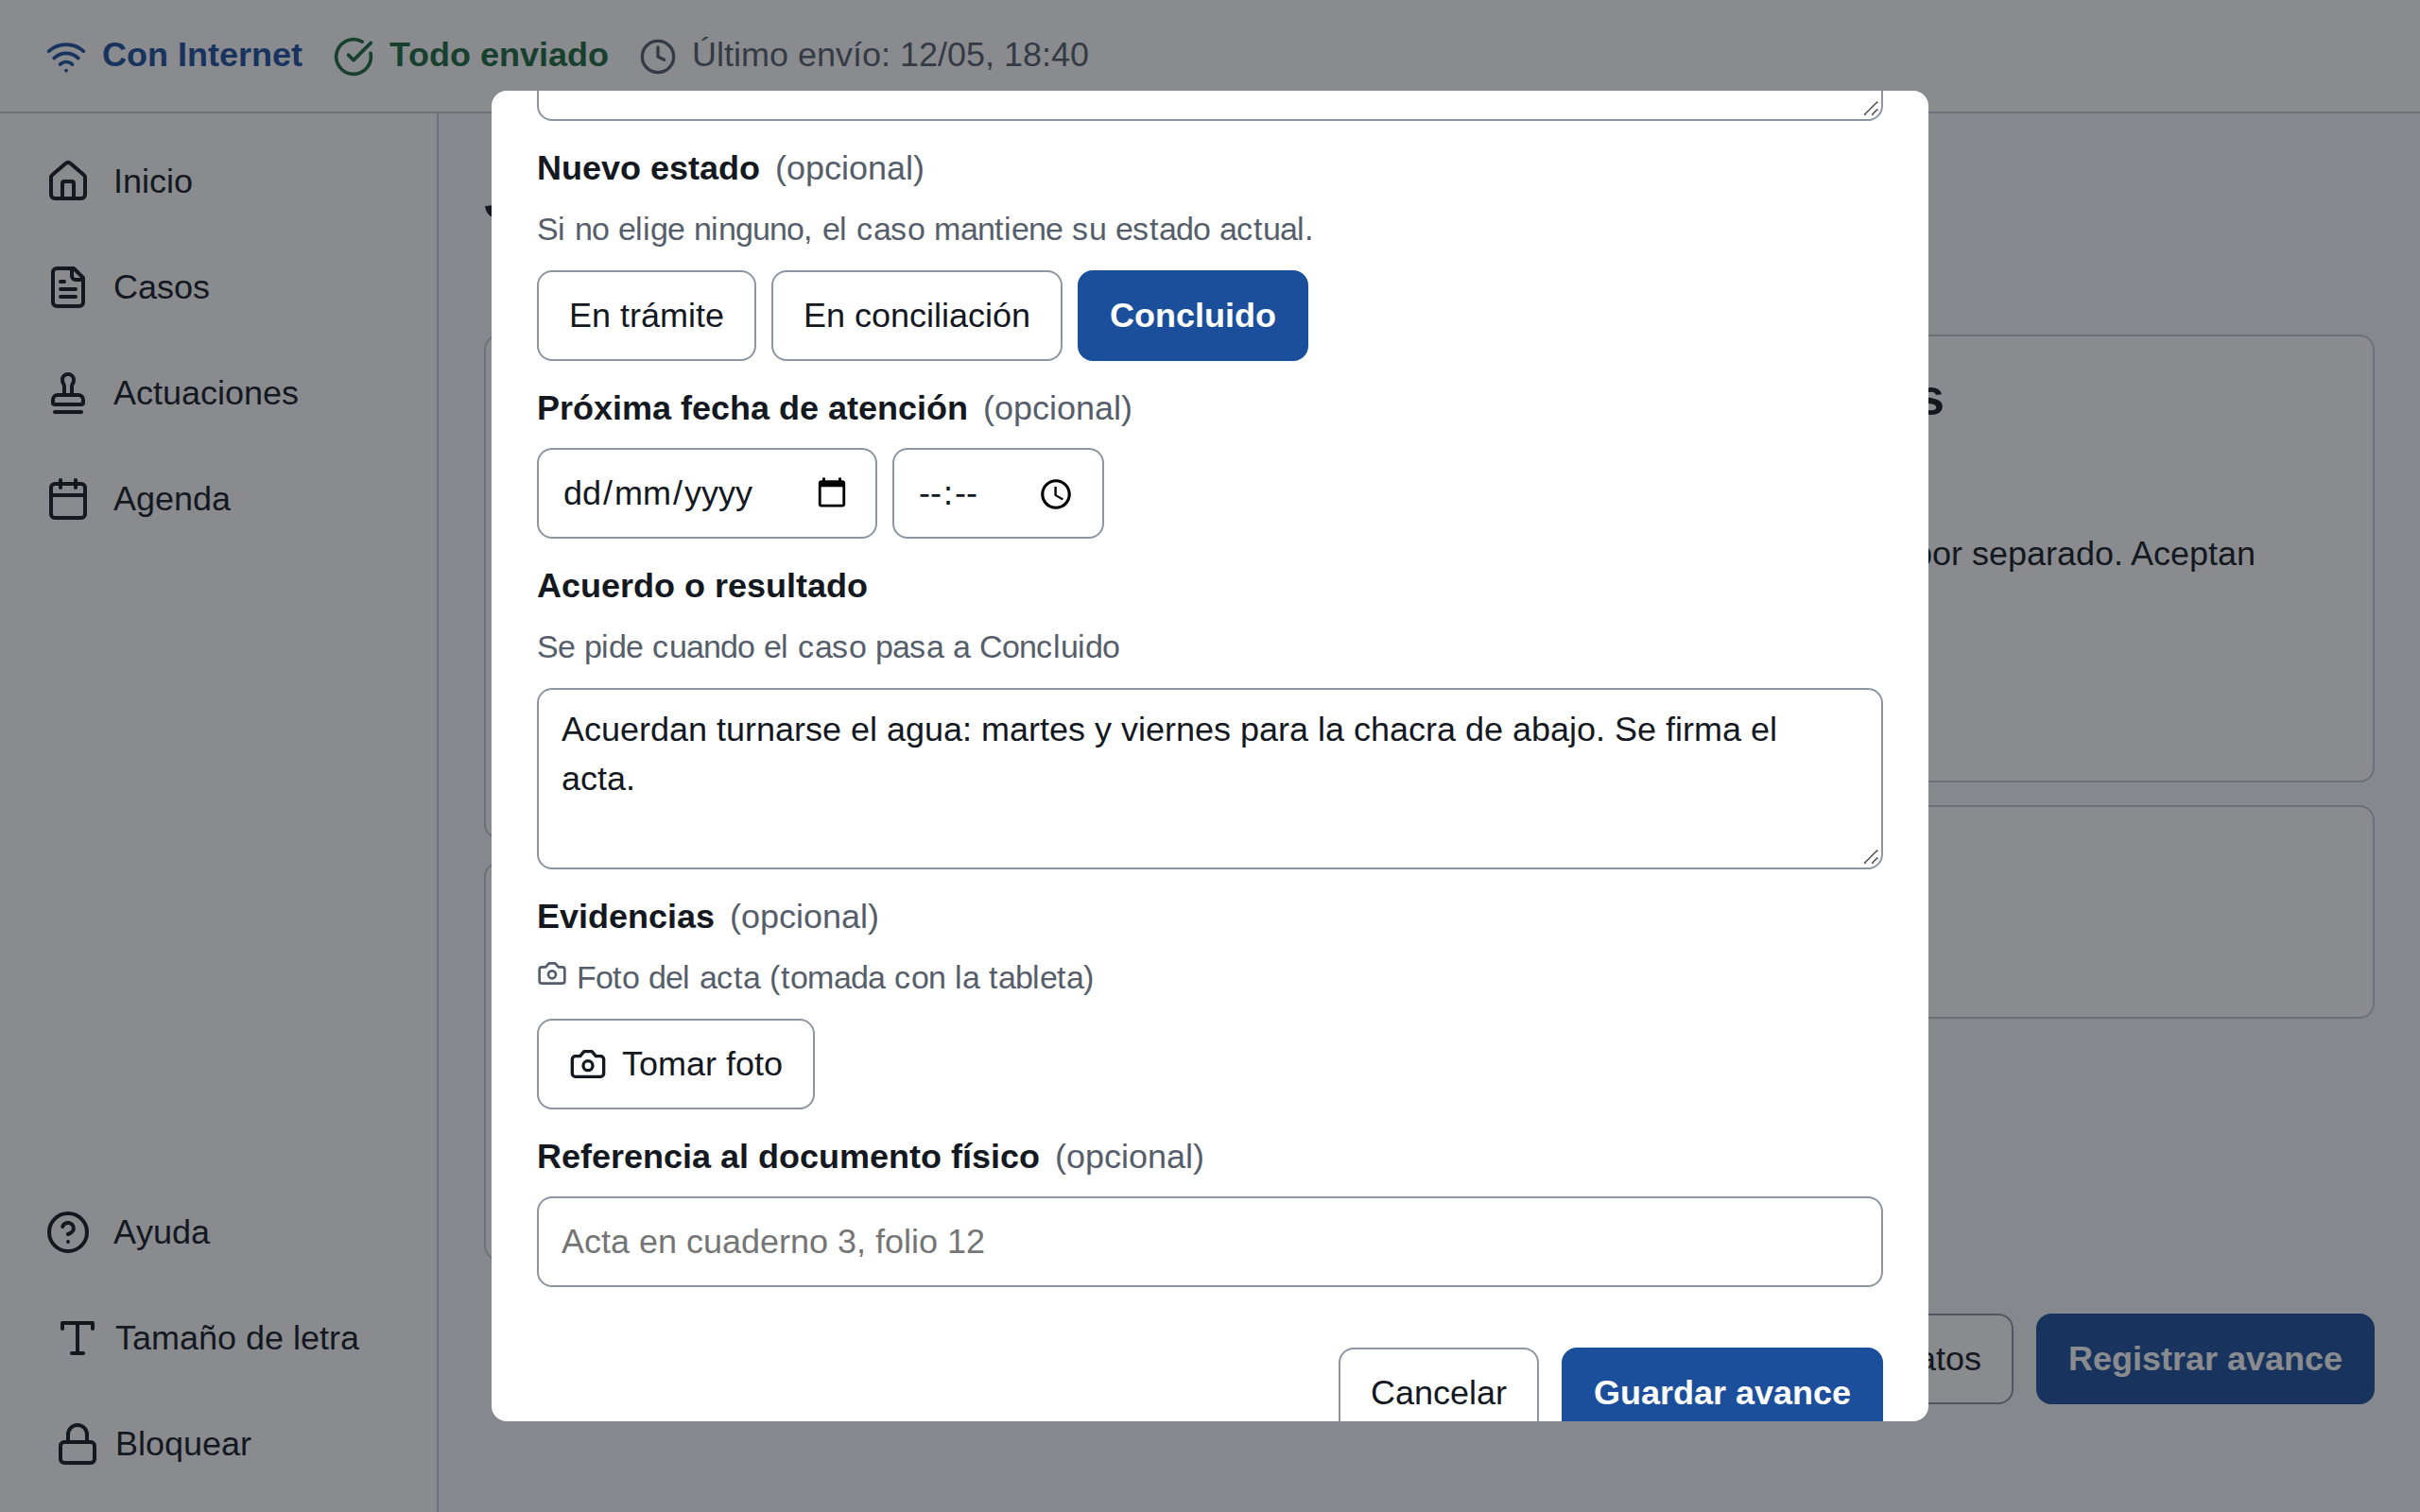
\includegraphics[width=0.82\linewidth]{capturas/FA-04_evidencia.png}
\caption{P-04 · 3. Evidencia del acta. La evidencia admite foto o referencia al cuaderno físico}
\end{figure}
\begin{figure}[H]\centering
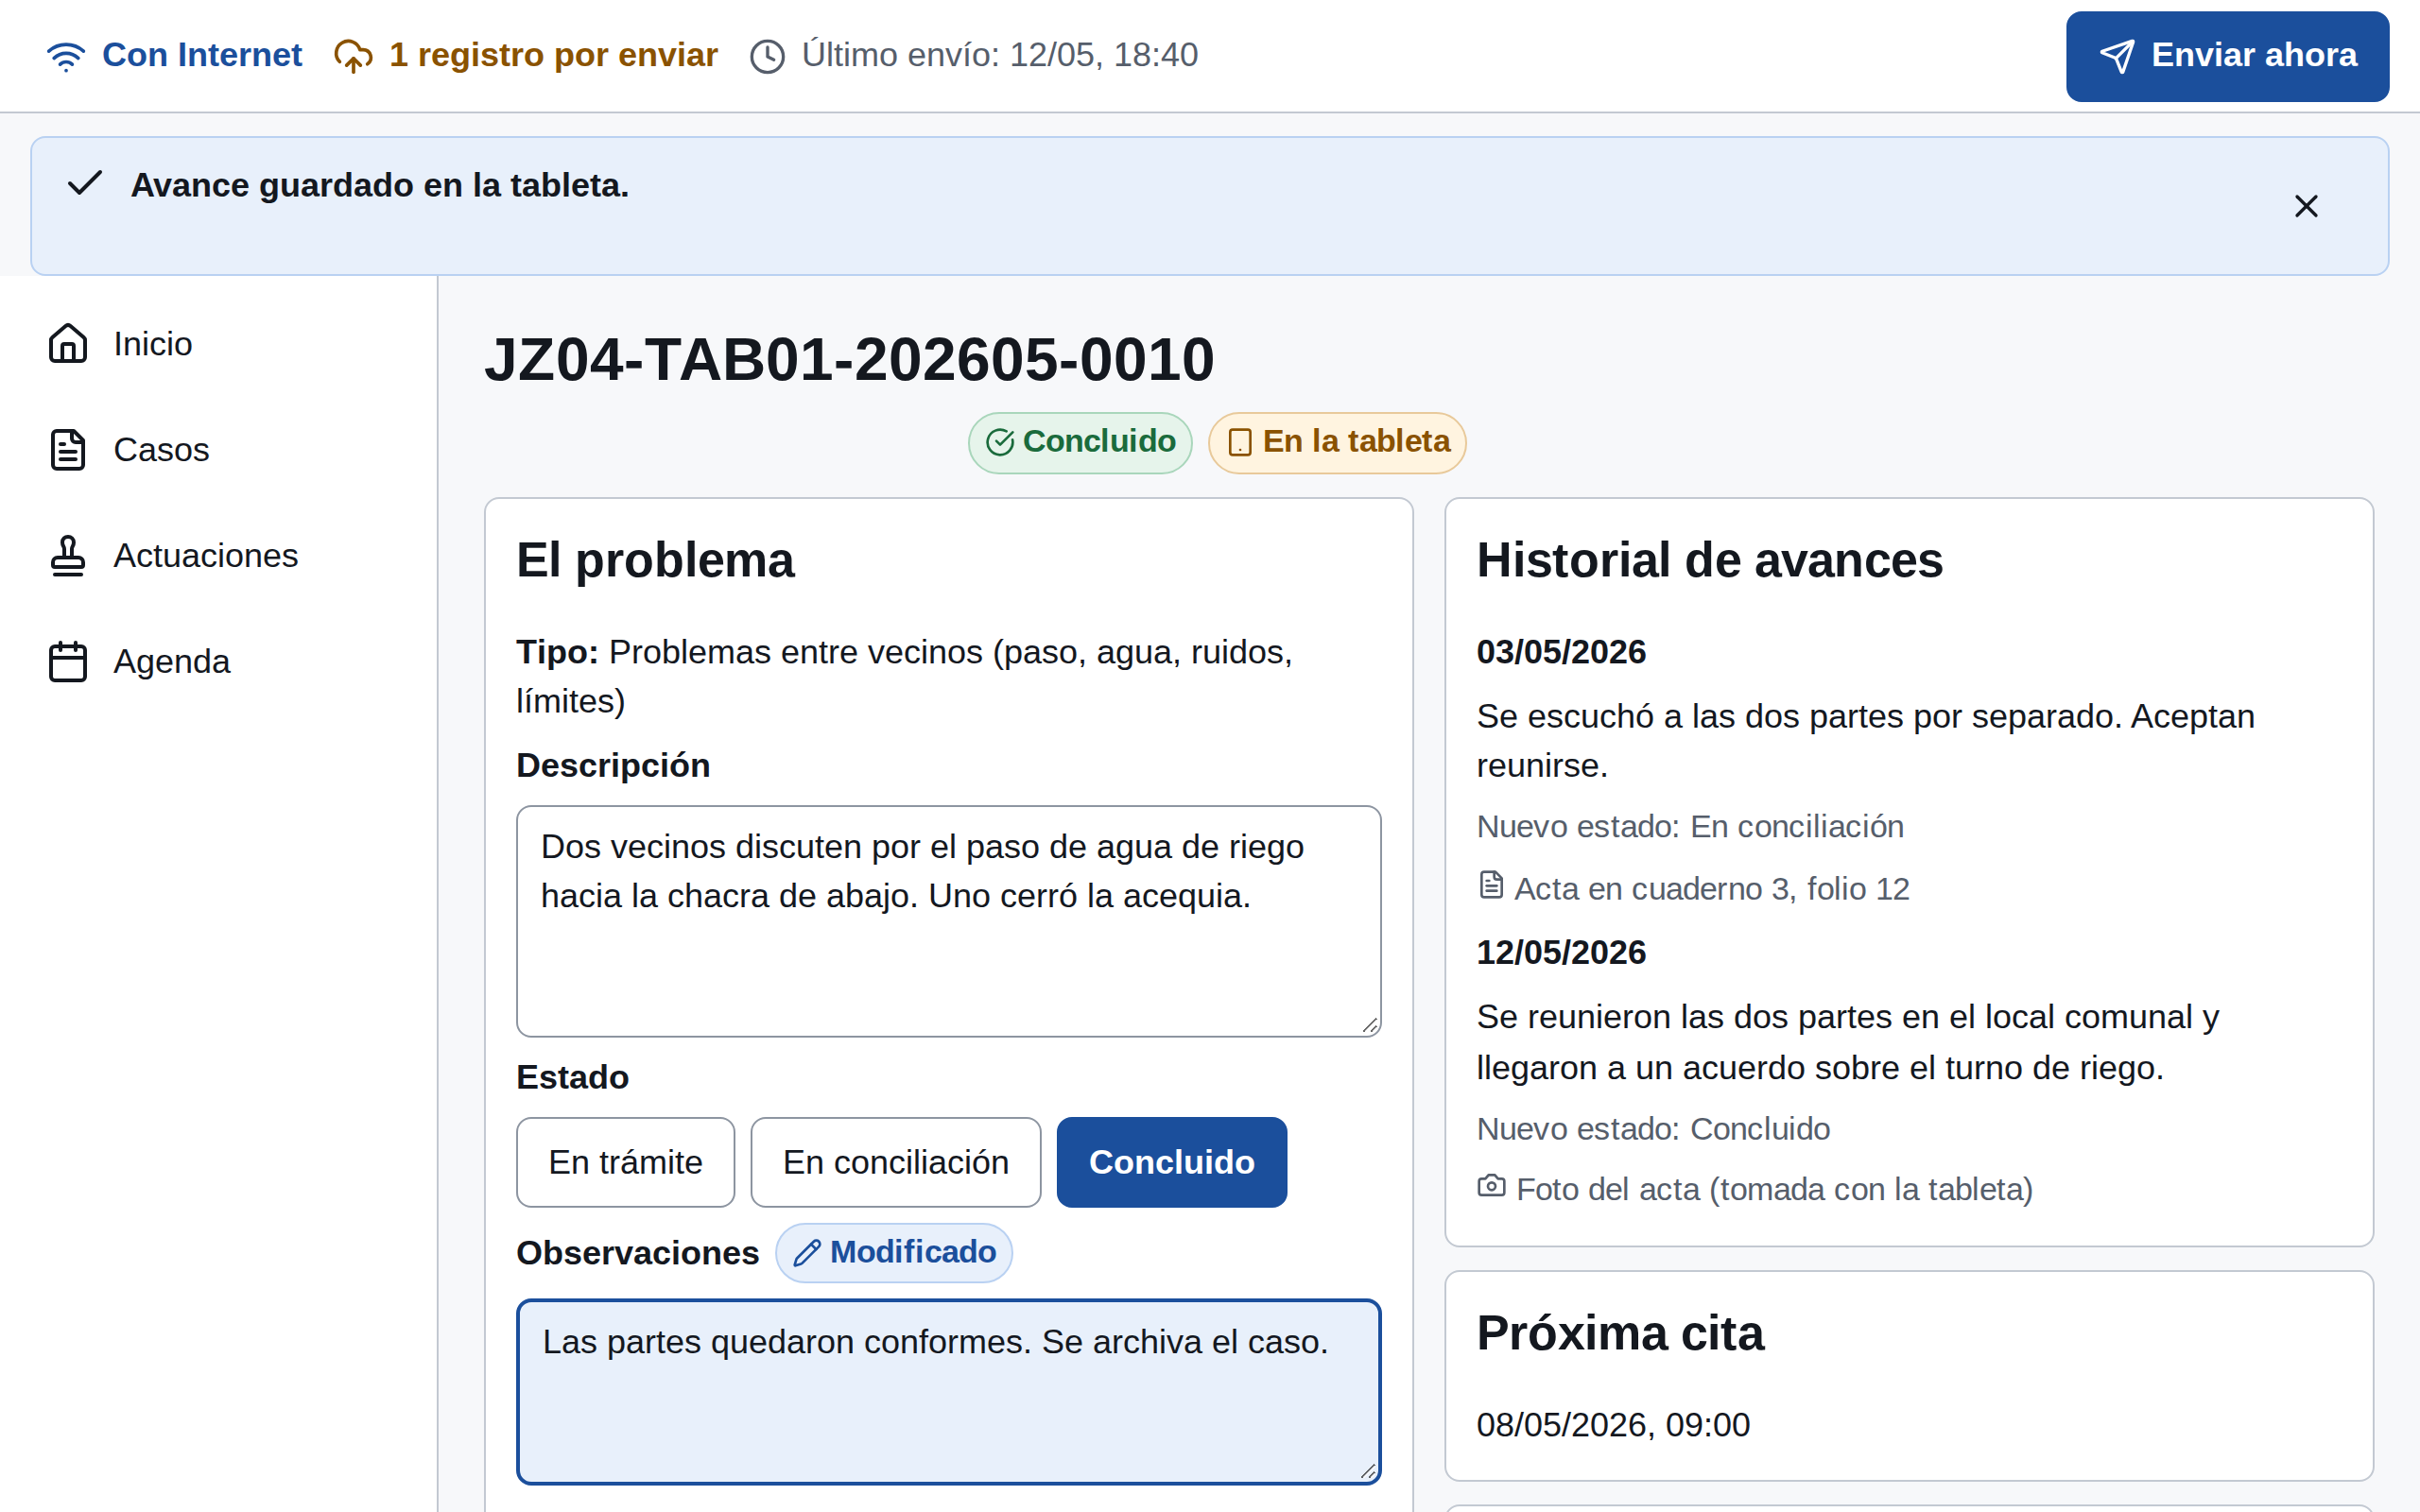
\includegraphics[width=0.82\linewidth]{capturas/FA-05_modificado.png}
\caption{P-04 · 4. Campo modificado con Deshacer. El campo cambiado se resalta y se puede deshacer antes de guardar}
\end{figure}
\begin{figure}[H]\centering
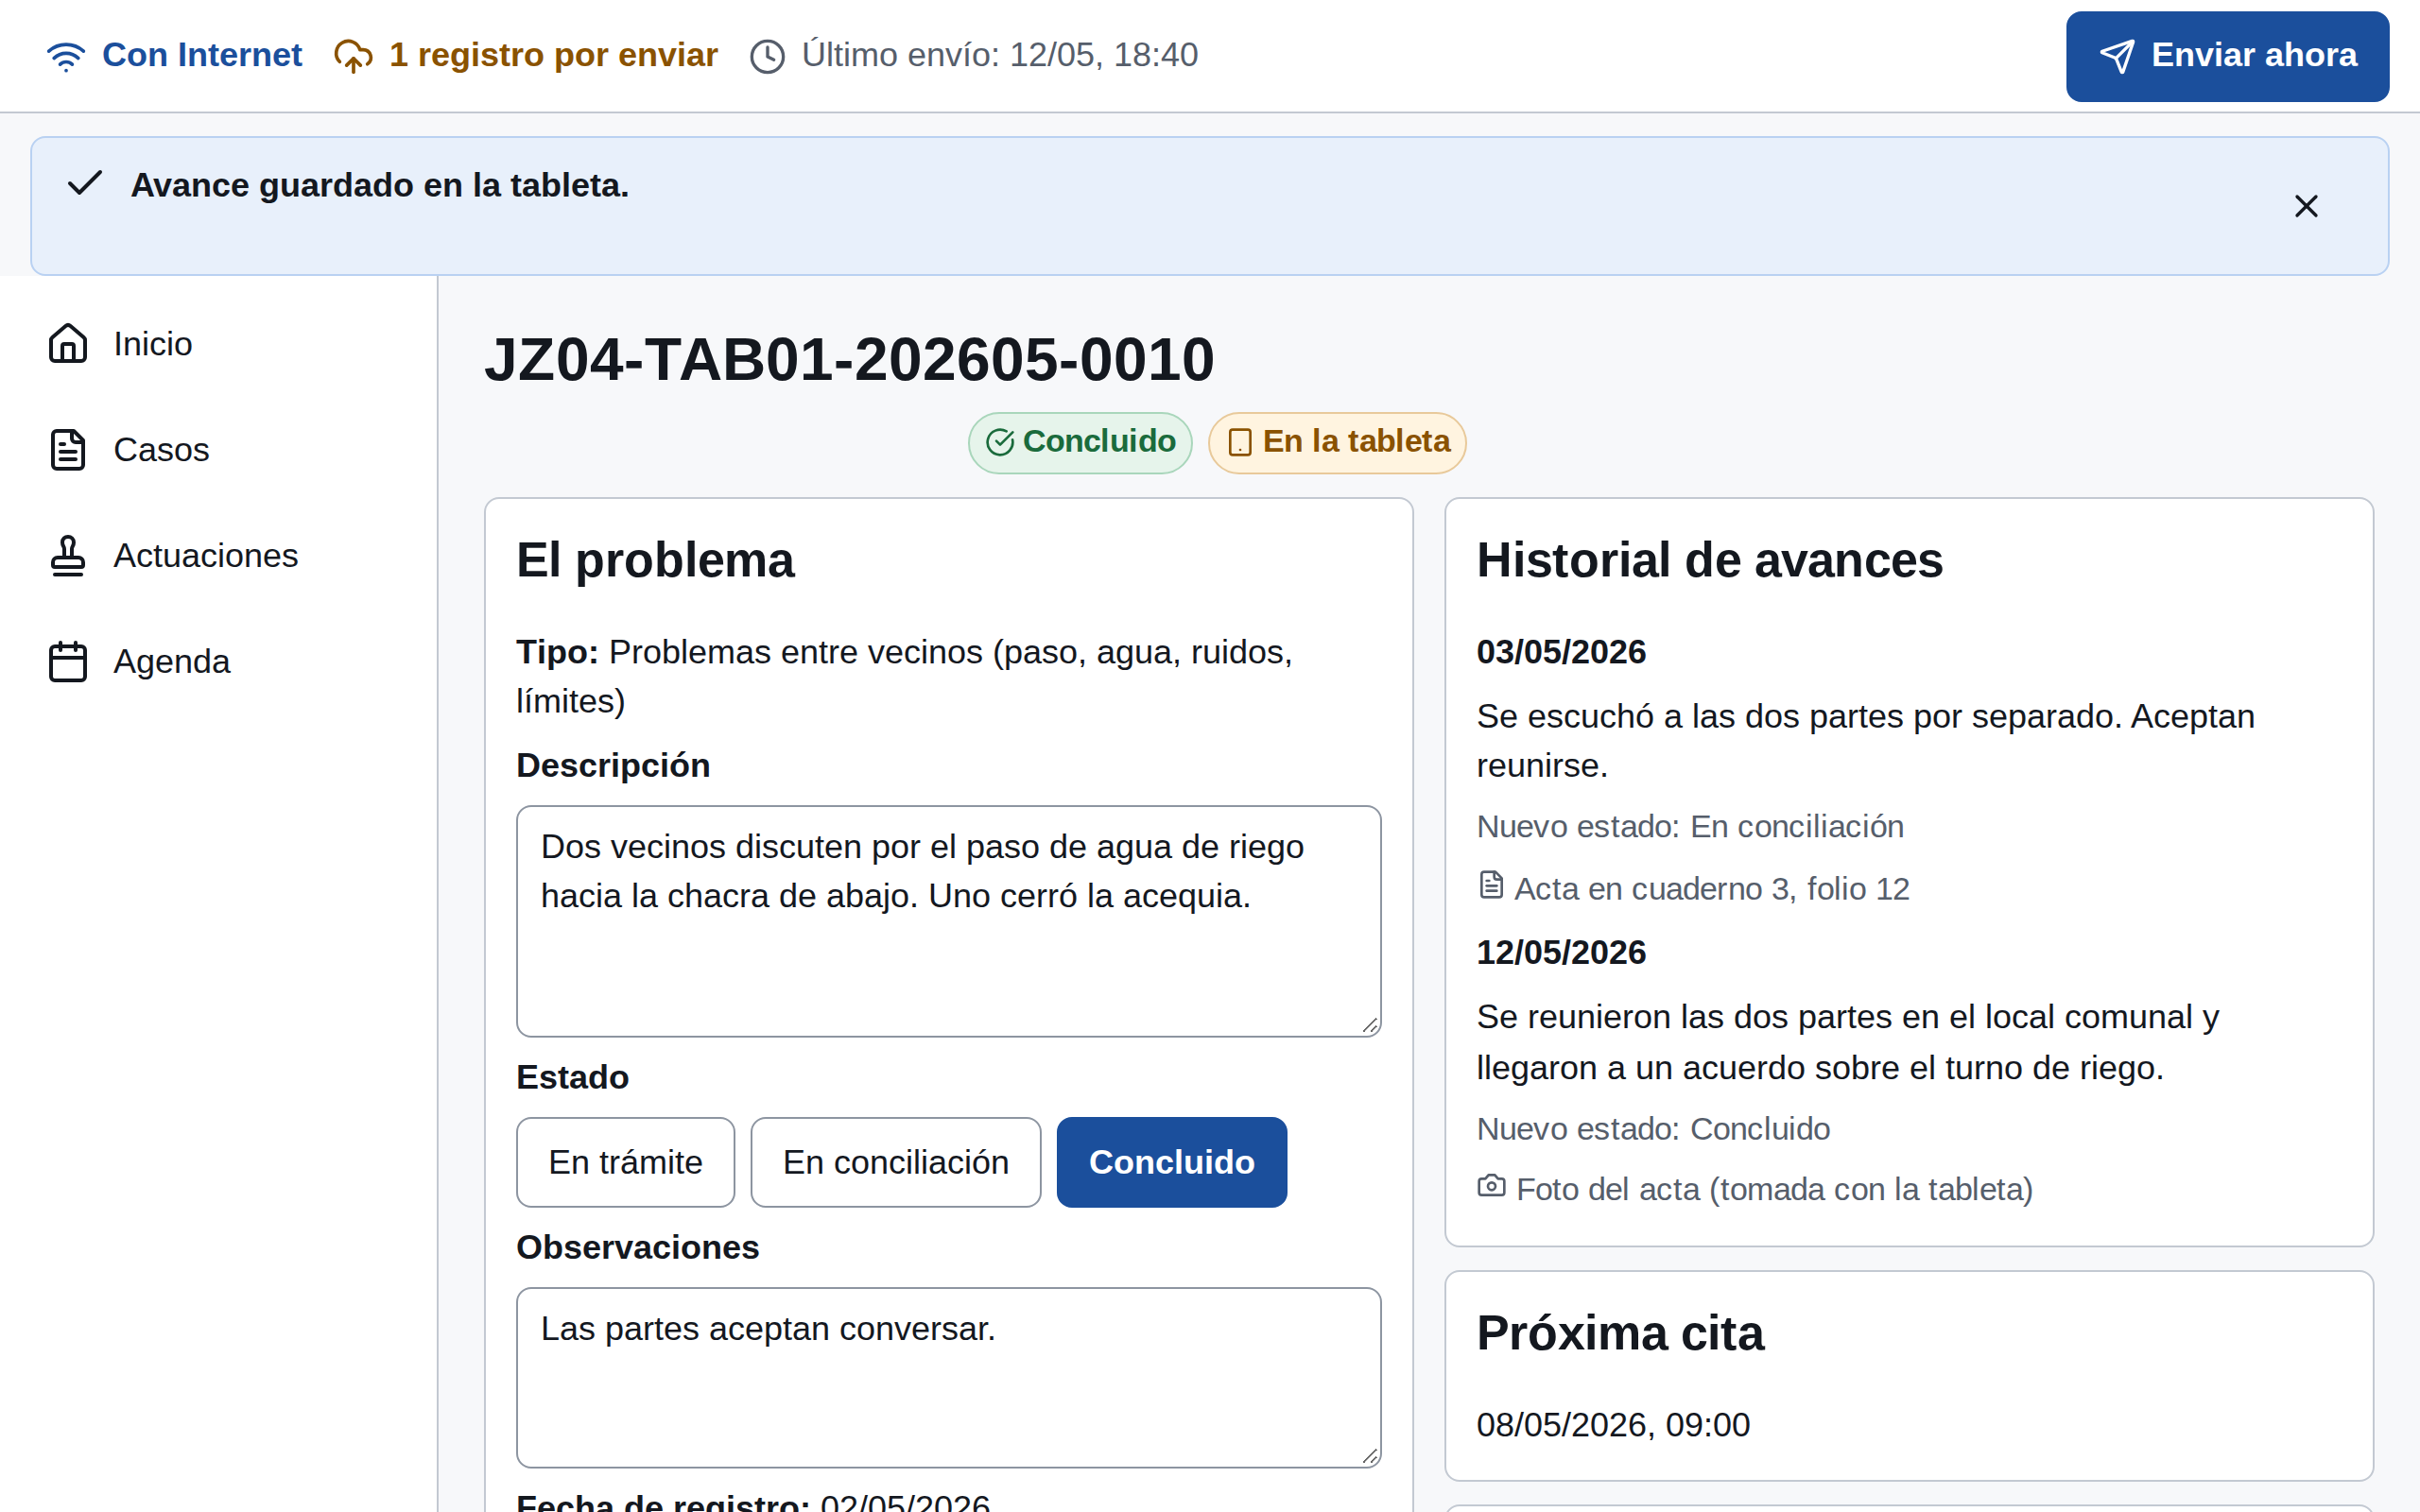
\includegraphics[width=0.82\linewidth]{capturas/FA-06_deshecho.png}
\caption{P-04 · 4. Deshecho. Deshacer devuelve el valor original sin perder el resto del trabajo}
\end{figure}
\begin{figure}[H]\centering
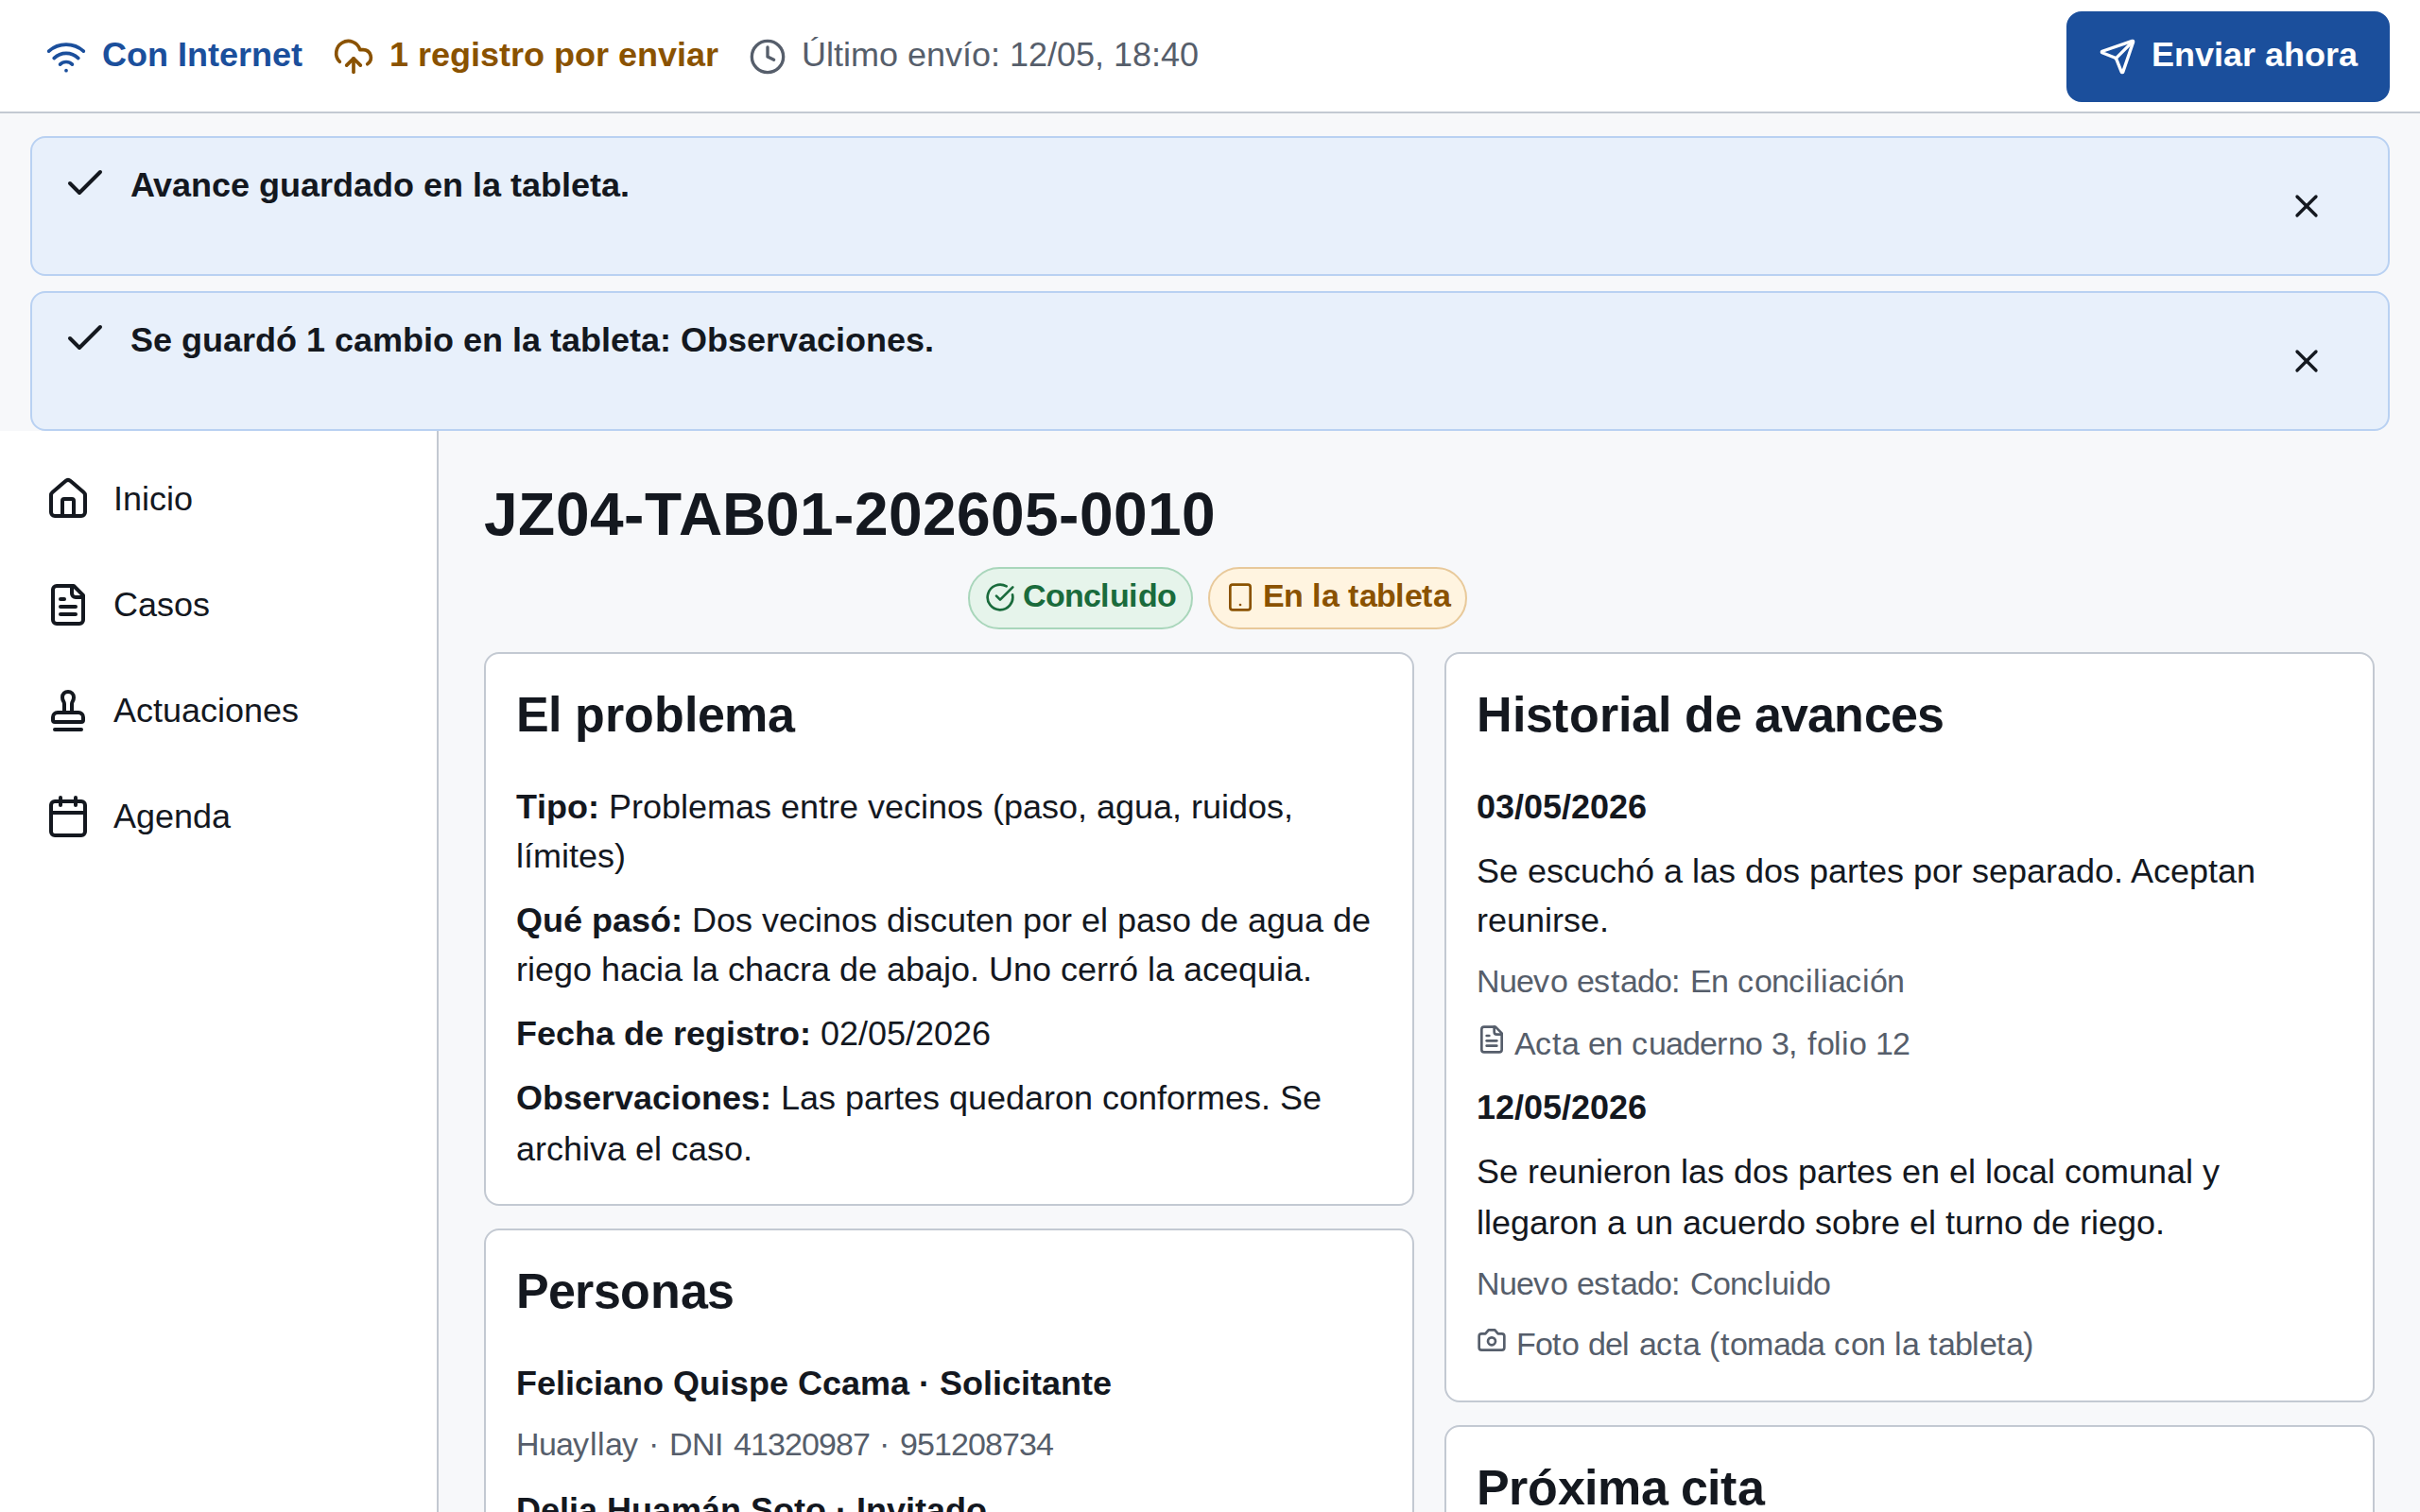
\includegraphics[width=0.82\linewidth]{capturas/FA-07_cambios-guardados.png}
\caption{P-04 · 4. Confirmación de cambios. La confirmación dice cuántos cambios se guardaron y en qué campos}
\end{figure}
\subsection{Flujo complementario B · Consultar y editar desde la computadora}
\begin{figure}[H]\centering
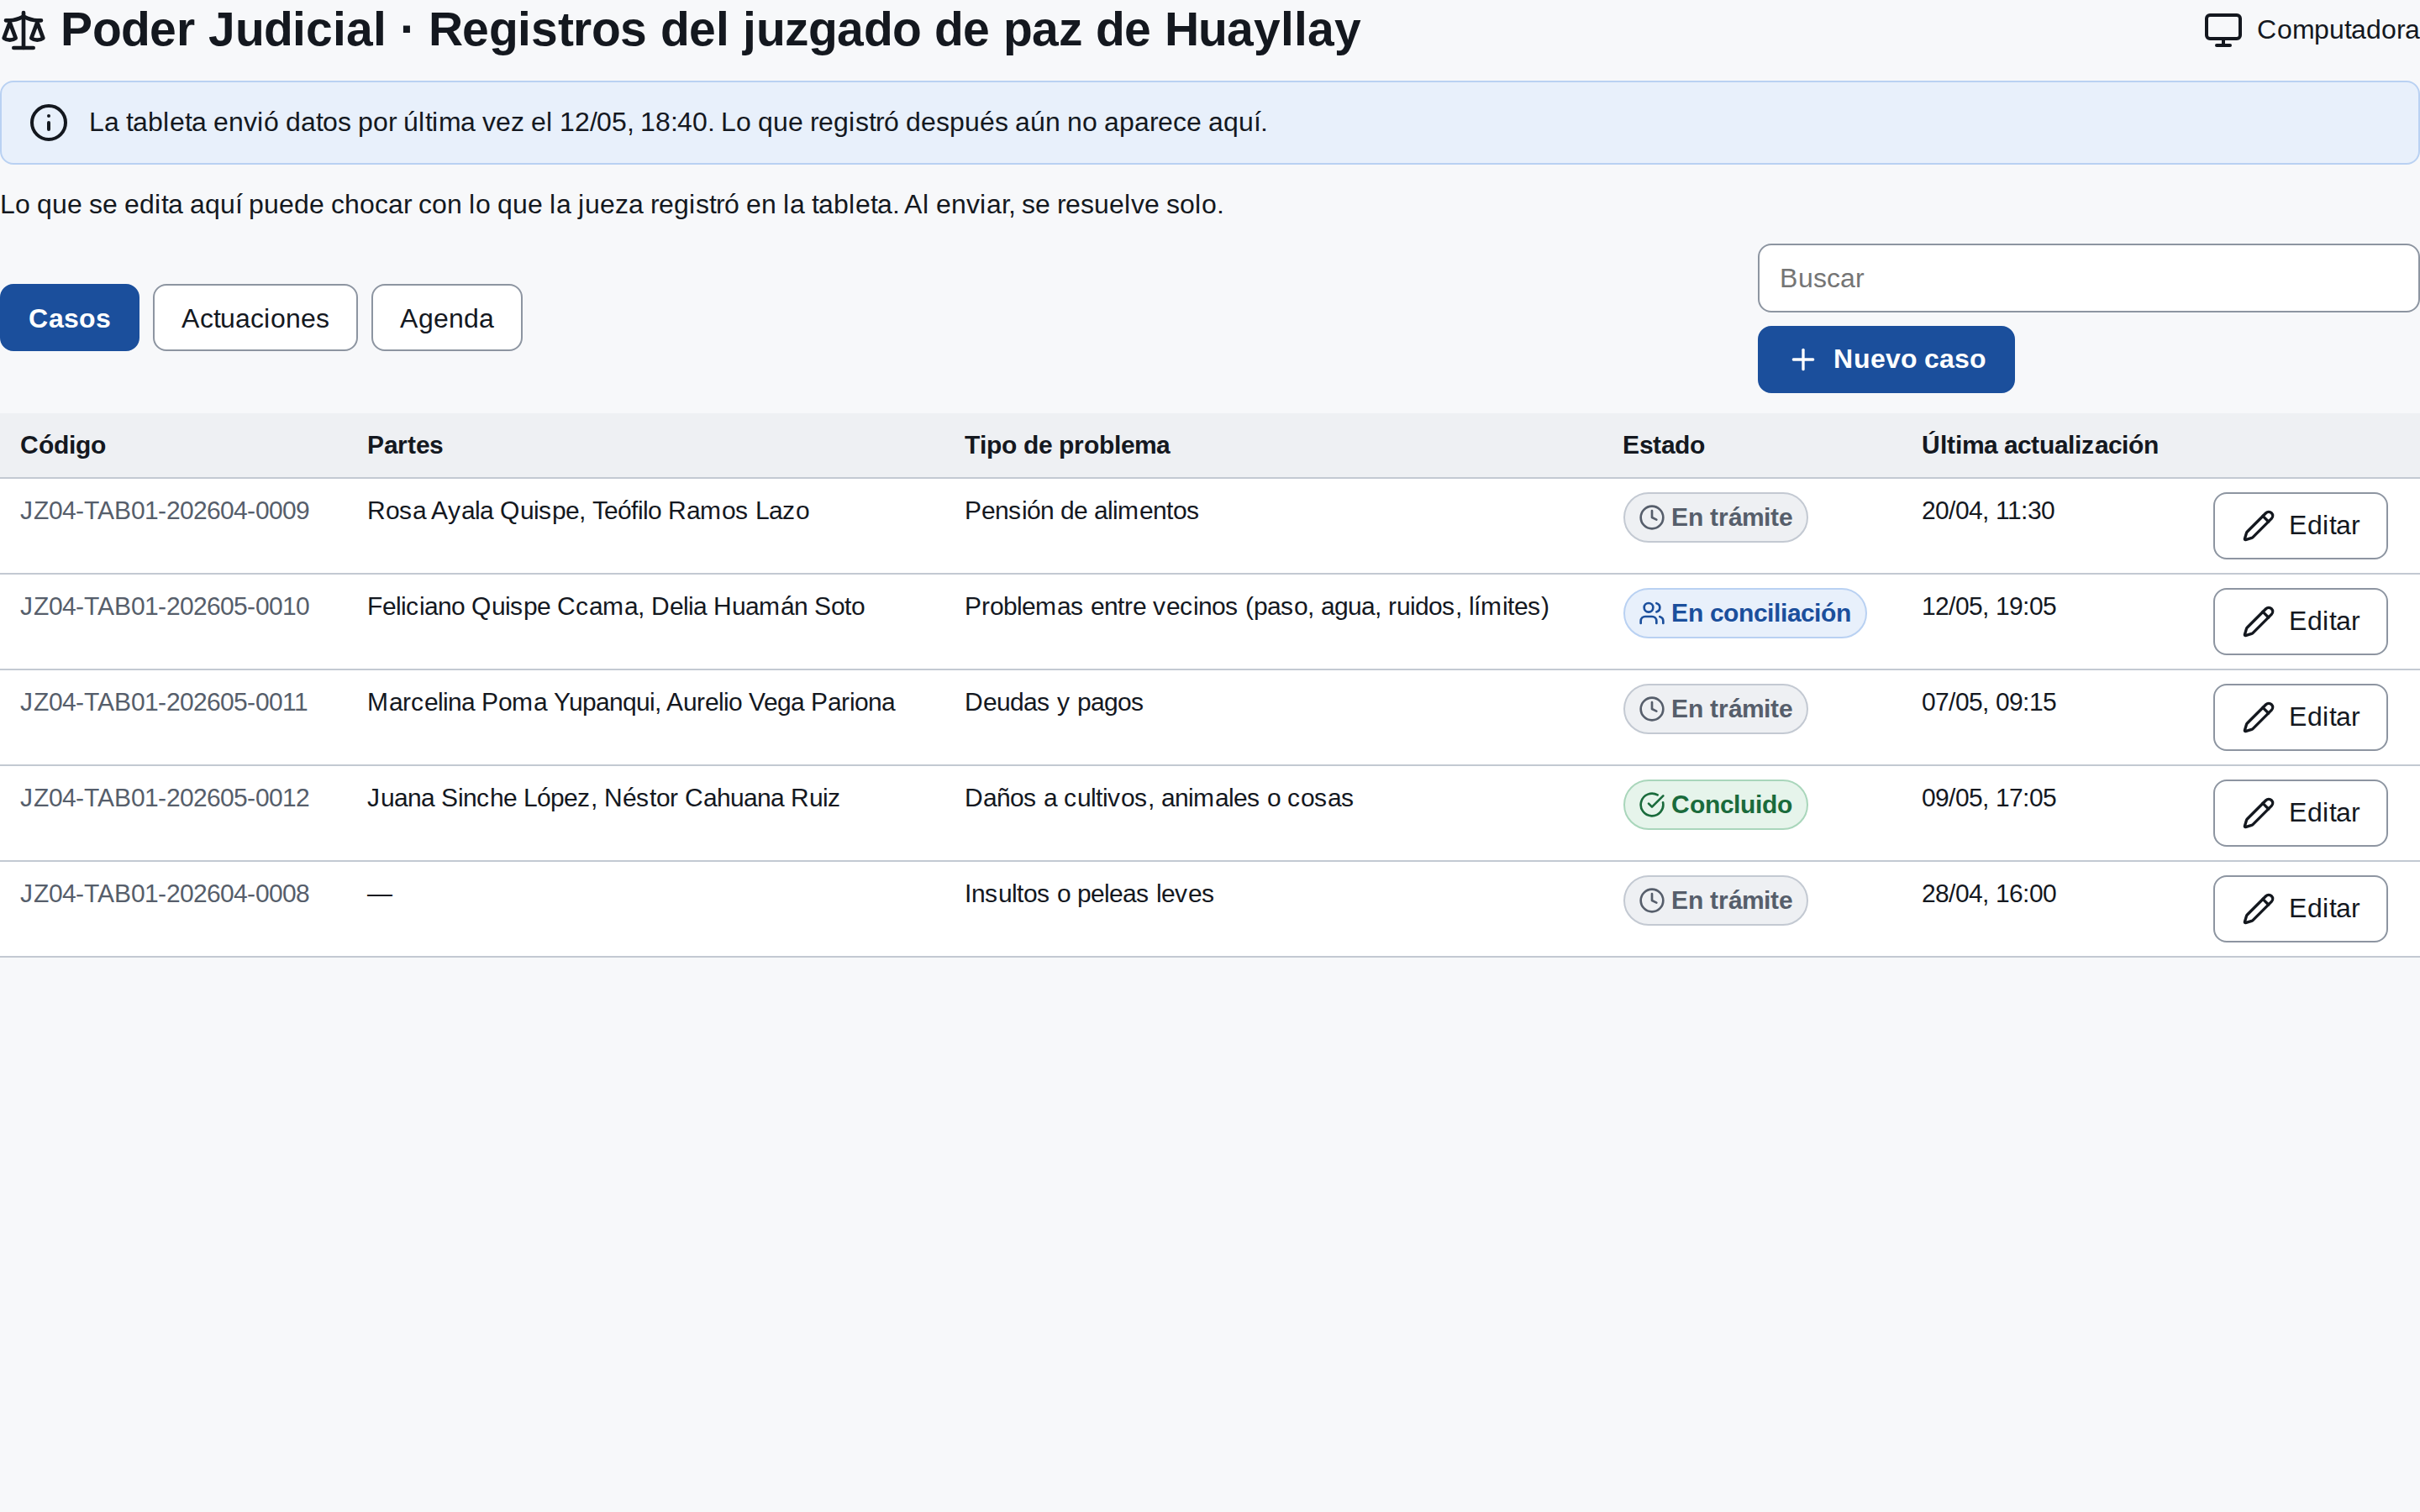
\includegraphics[width=0.82\linewidth]{capturas/FB-01_pc-casos.png}
\caption{P-10 · 1. Datos que ya llegaron. Aviso del último envío de la tableta, sin afirmar cuántos registros quedan pendientes}
\end{figure}
\begin{figure}[H]\centering
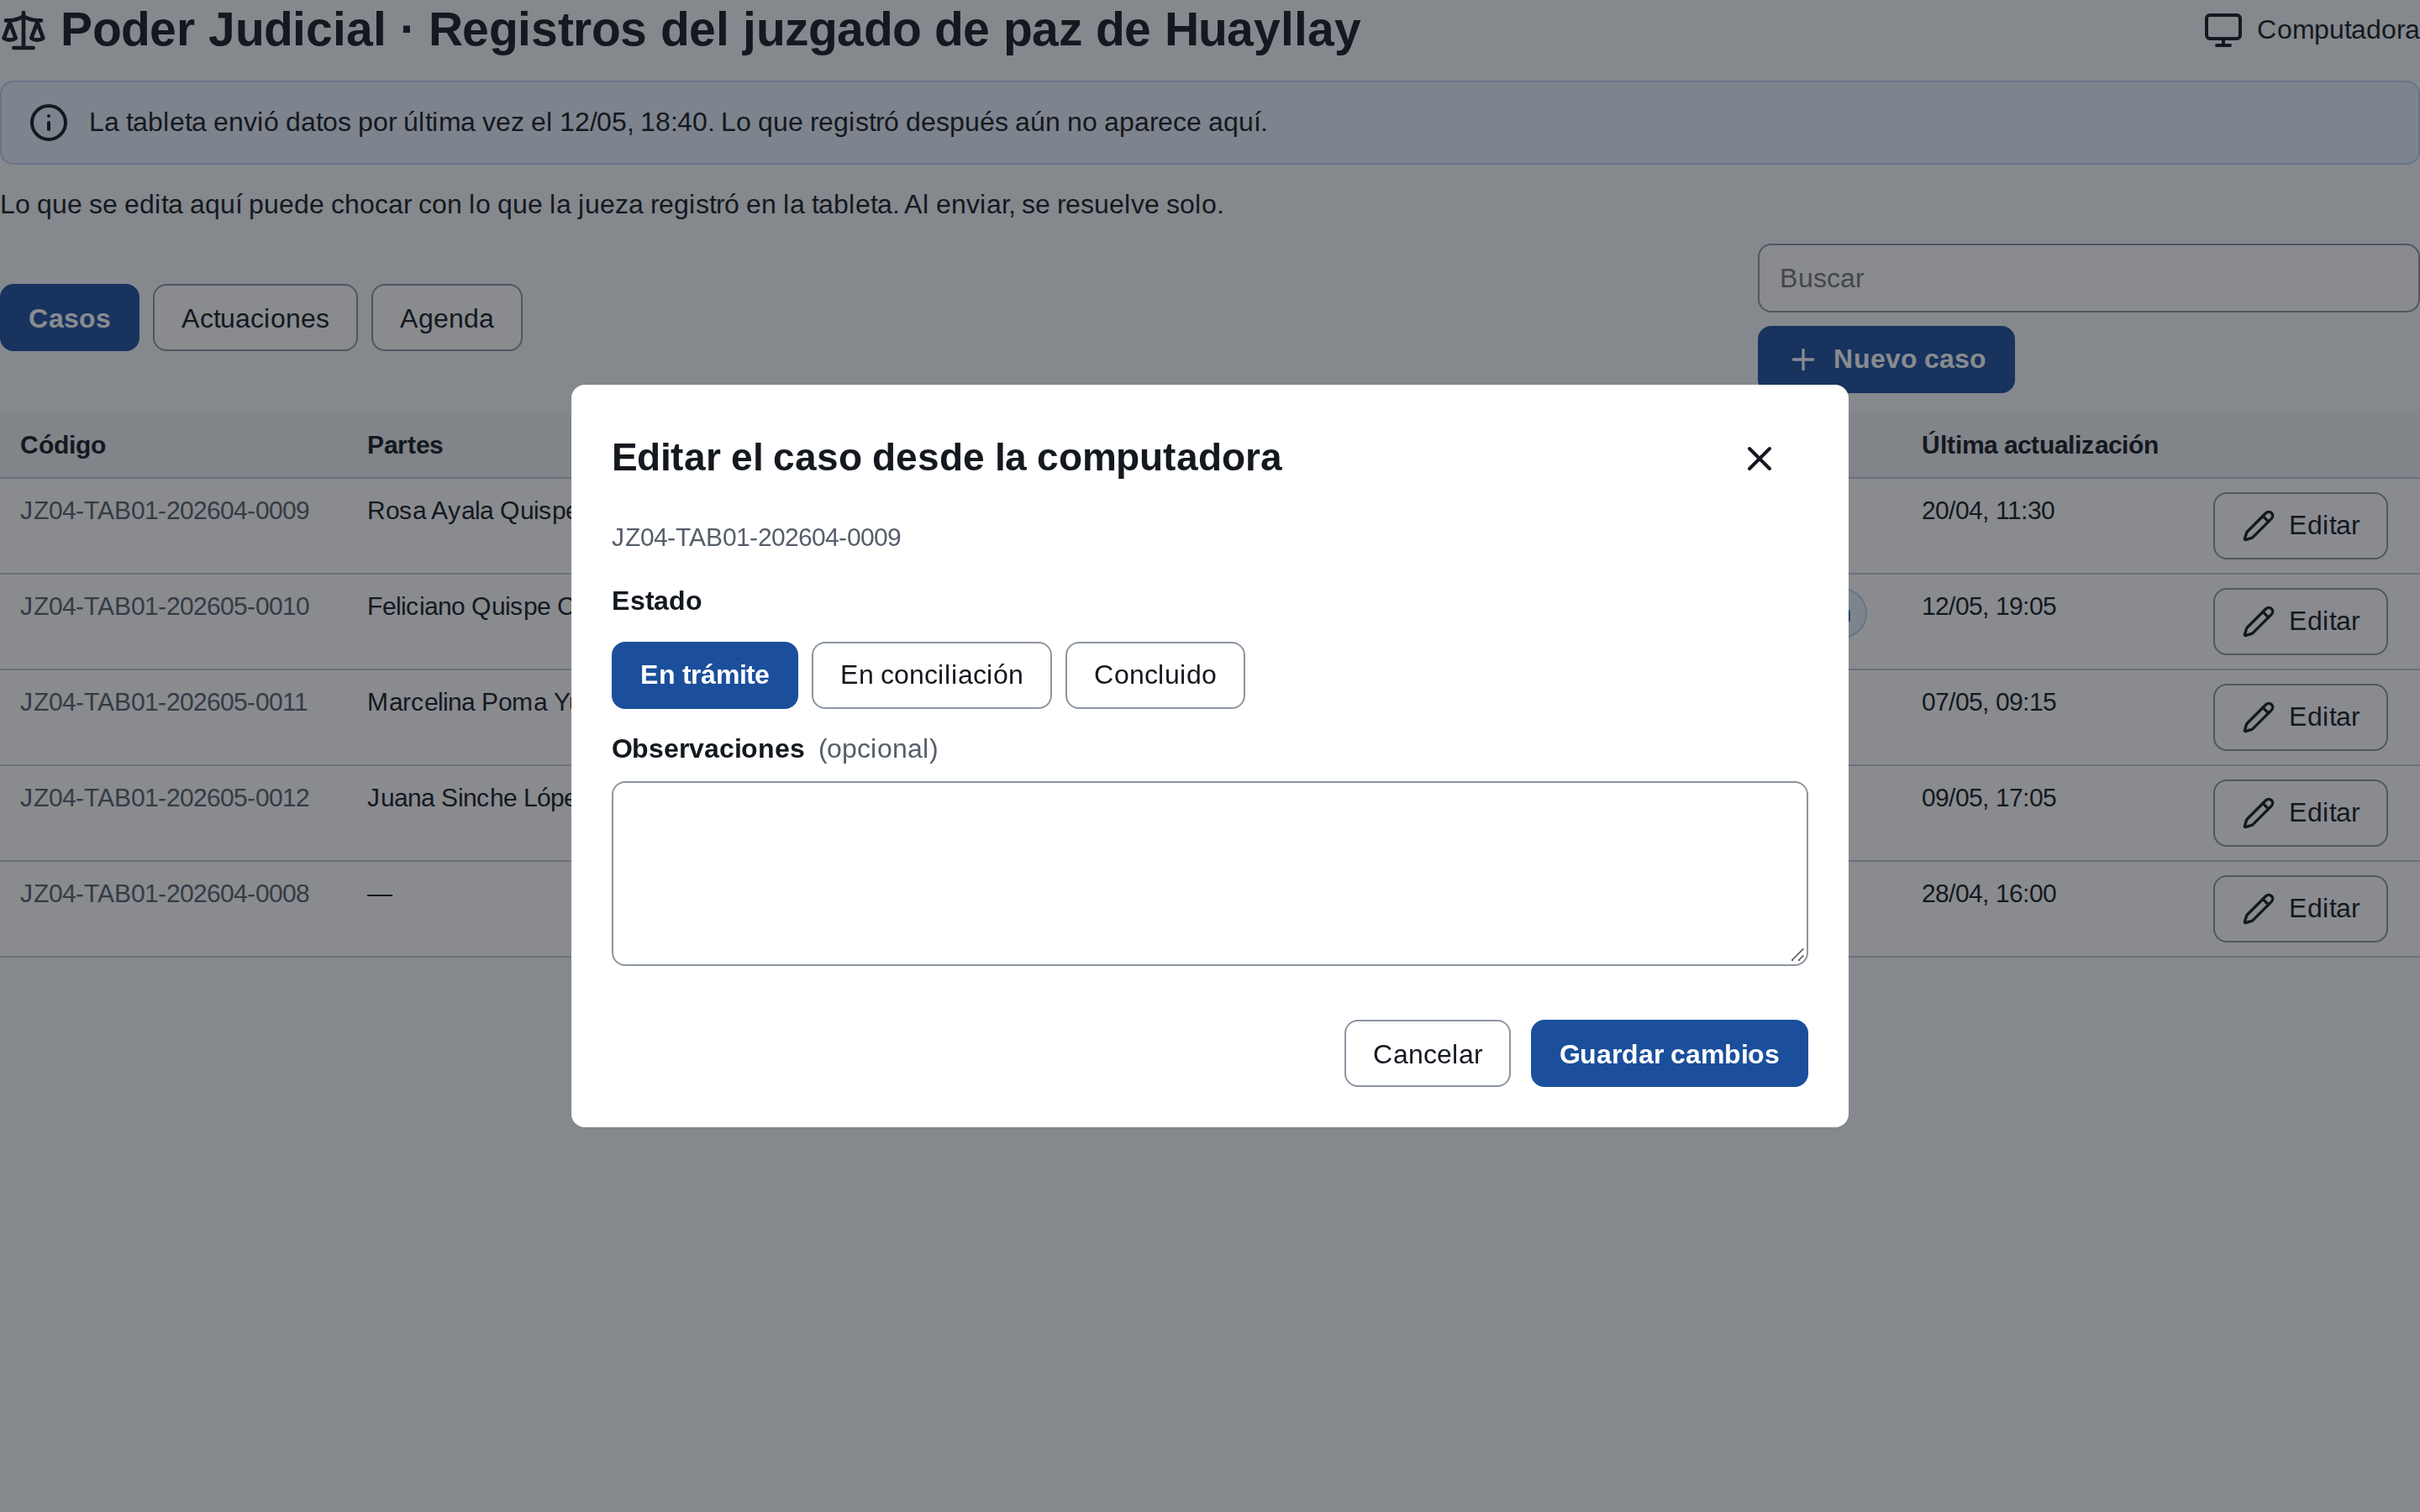
\includegraphics[width=0.82\linewidth]{capturas/FB-02_pc-editar.png}
\caption{P-10 · 2. Edición desde la computadora. Desde la computadora se puede editar, y de ahí nacen los conflictos de P-09}
\end{figure}


\section{Estados especiales}

Batería baja, tamaño de letra y orientación de la tableta.

Al 20\,\% y al 10\,\% de batería la aplicación avisa recordando que lo registrado ya está guardado, e incluye \textbf{Enviar ahora} si hay Internet y quedan pendientes. En zonas rurales la energía es tan escasa como la conexión, y el aviso reduce la ansiedad por pérdida de datos.

El tamaño de letra se cambia desde el menú con tres opciones (18, 21 y 24 píxeles) y se recuerda entre sesiones, por los usuarios mayores con presbicia. Los tres tamaños pasan la medición de objetivos táctiles de la sección de factores humanos.

La aplicación se usa solo en horizontal: el menú lateral, los formularios de tres pasos y la vista semanal necesitan ancho, y un solo diseño evita que la jueza tenga que reaprender dónde está cada cosa. Si se gira la tableta, aparece «Gire la tableta para usarla de lado» con una ilustración.

\begin{figure}[H]\centering
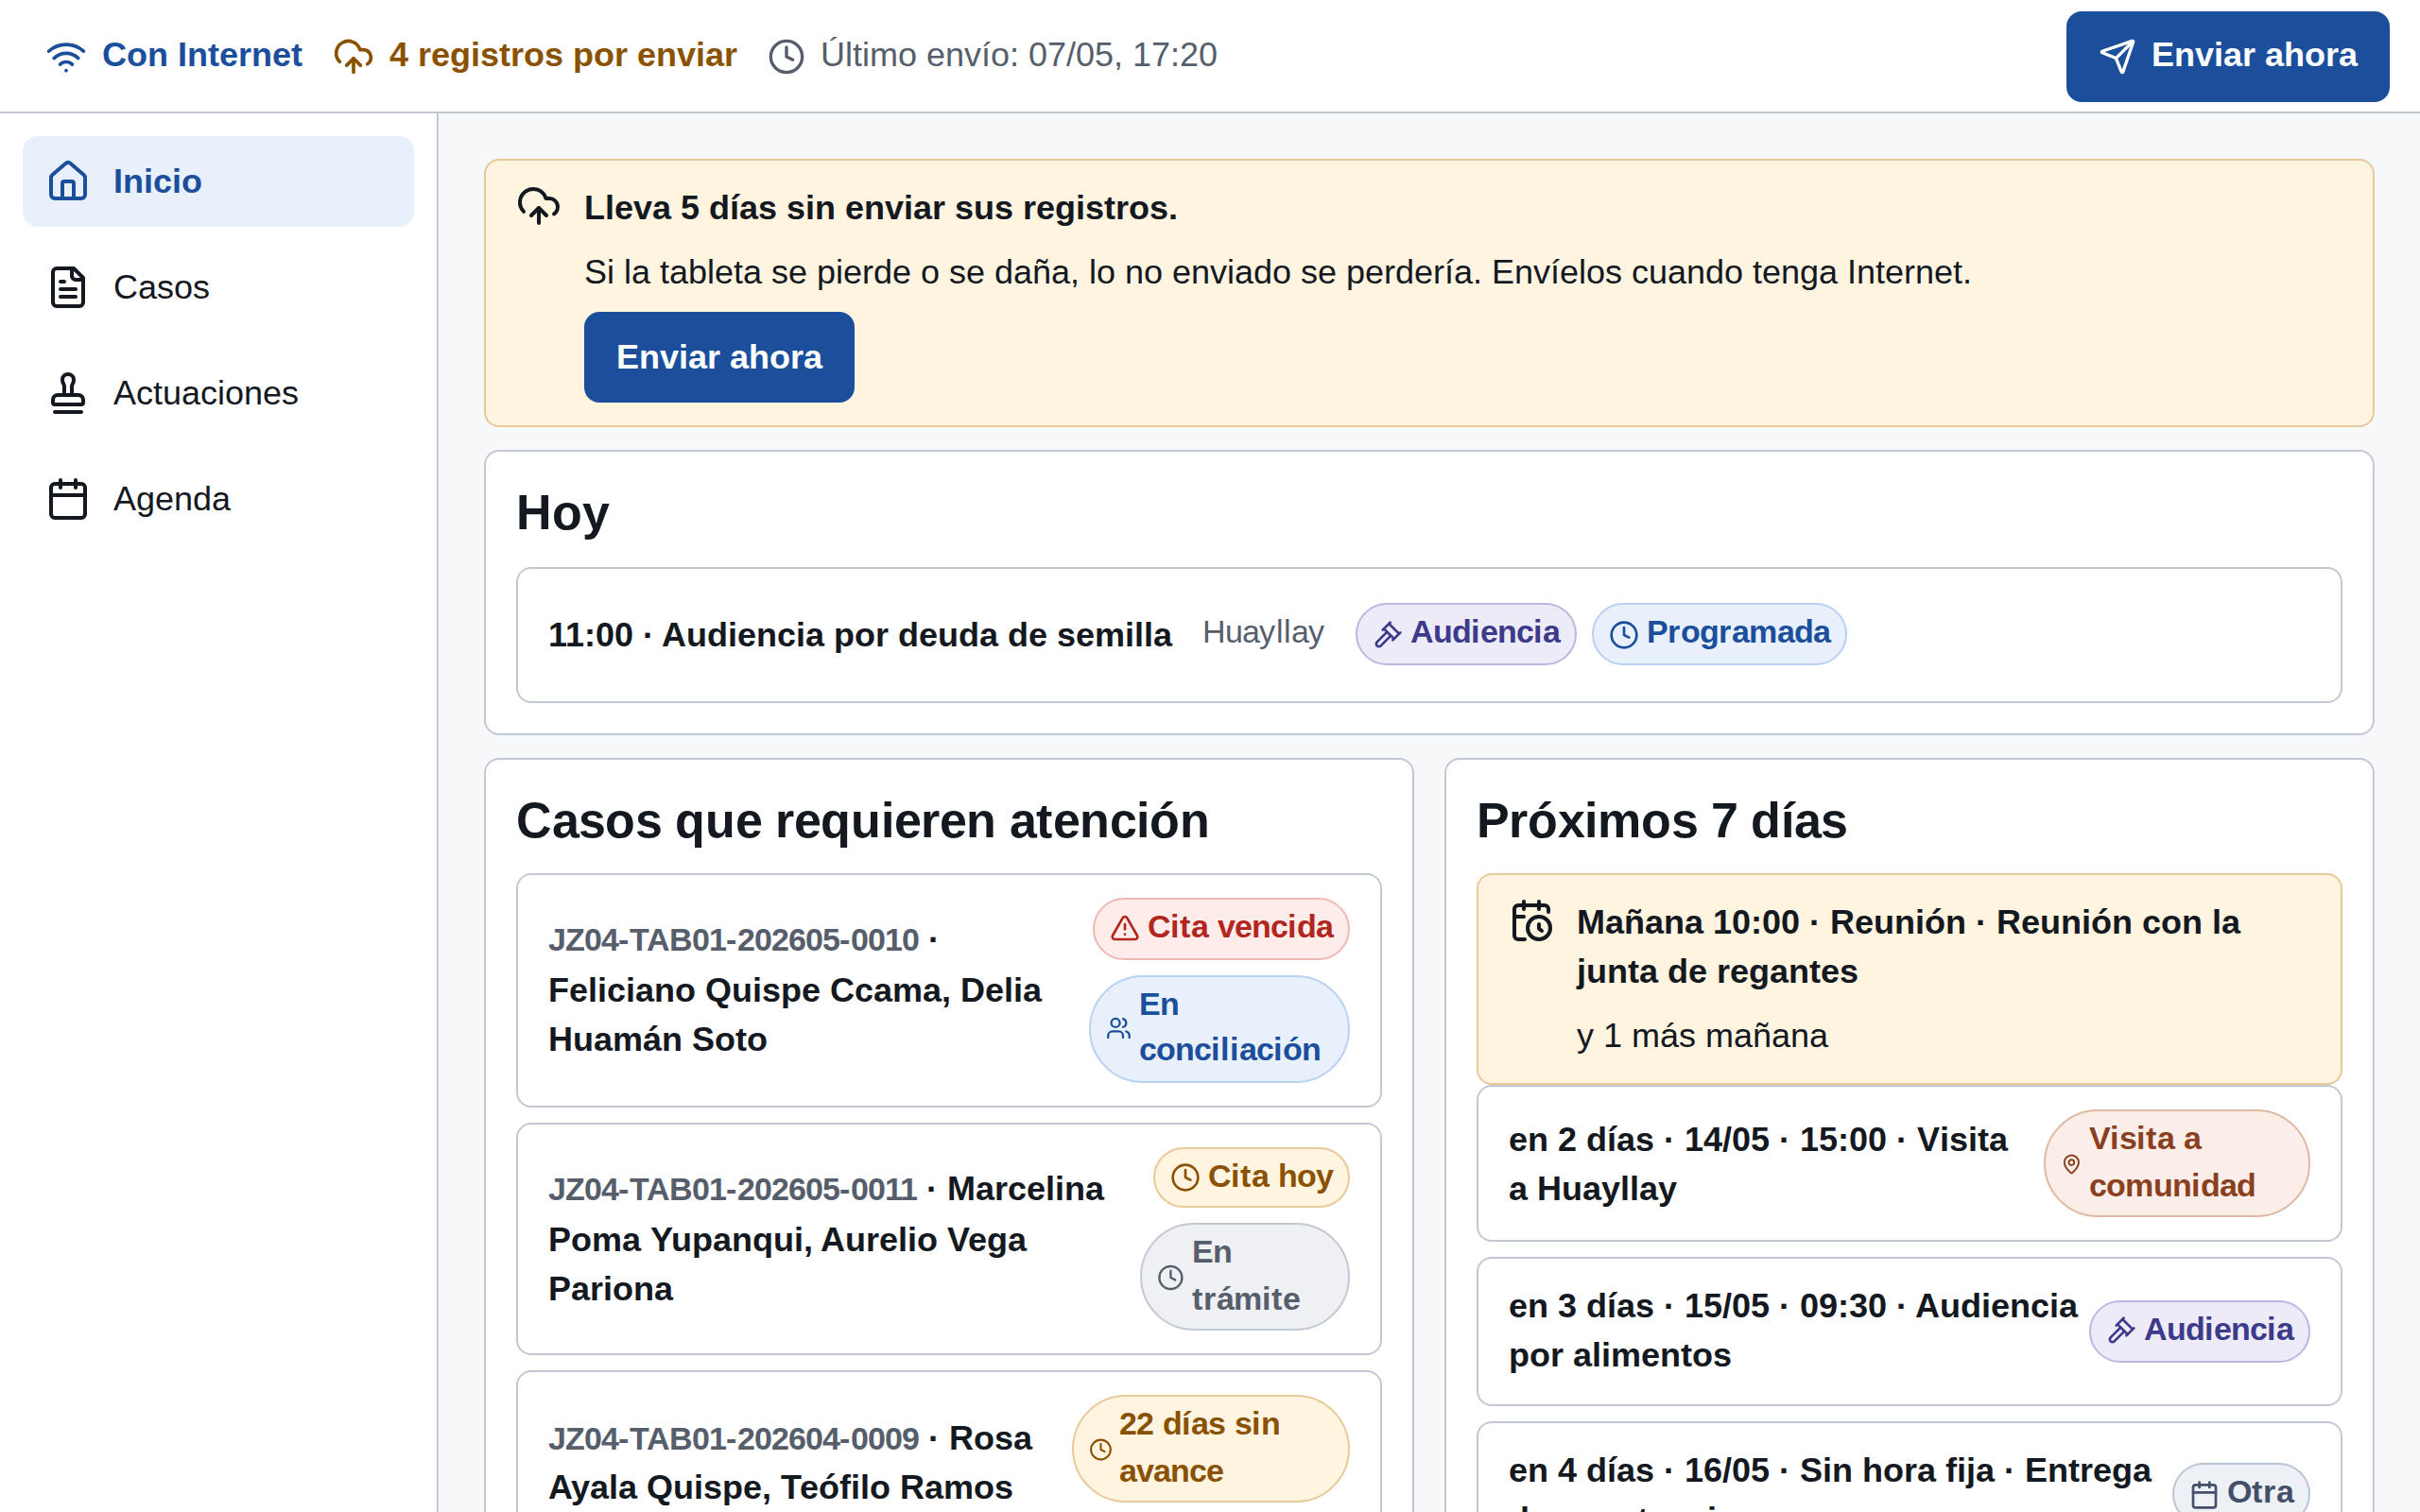
\includegraphics[width=0.78\linewidth]{capturas/X-01_recordatorio-dias.png}
\caption{P-01 · Días sin enviar. Recordatorio con el riesgo explicado en una frase, no una alarma}
\end{figure}
\begin{figure}[H]\centering
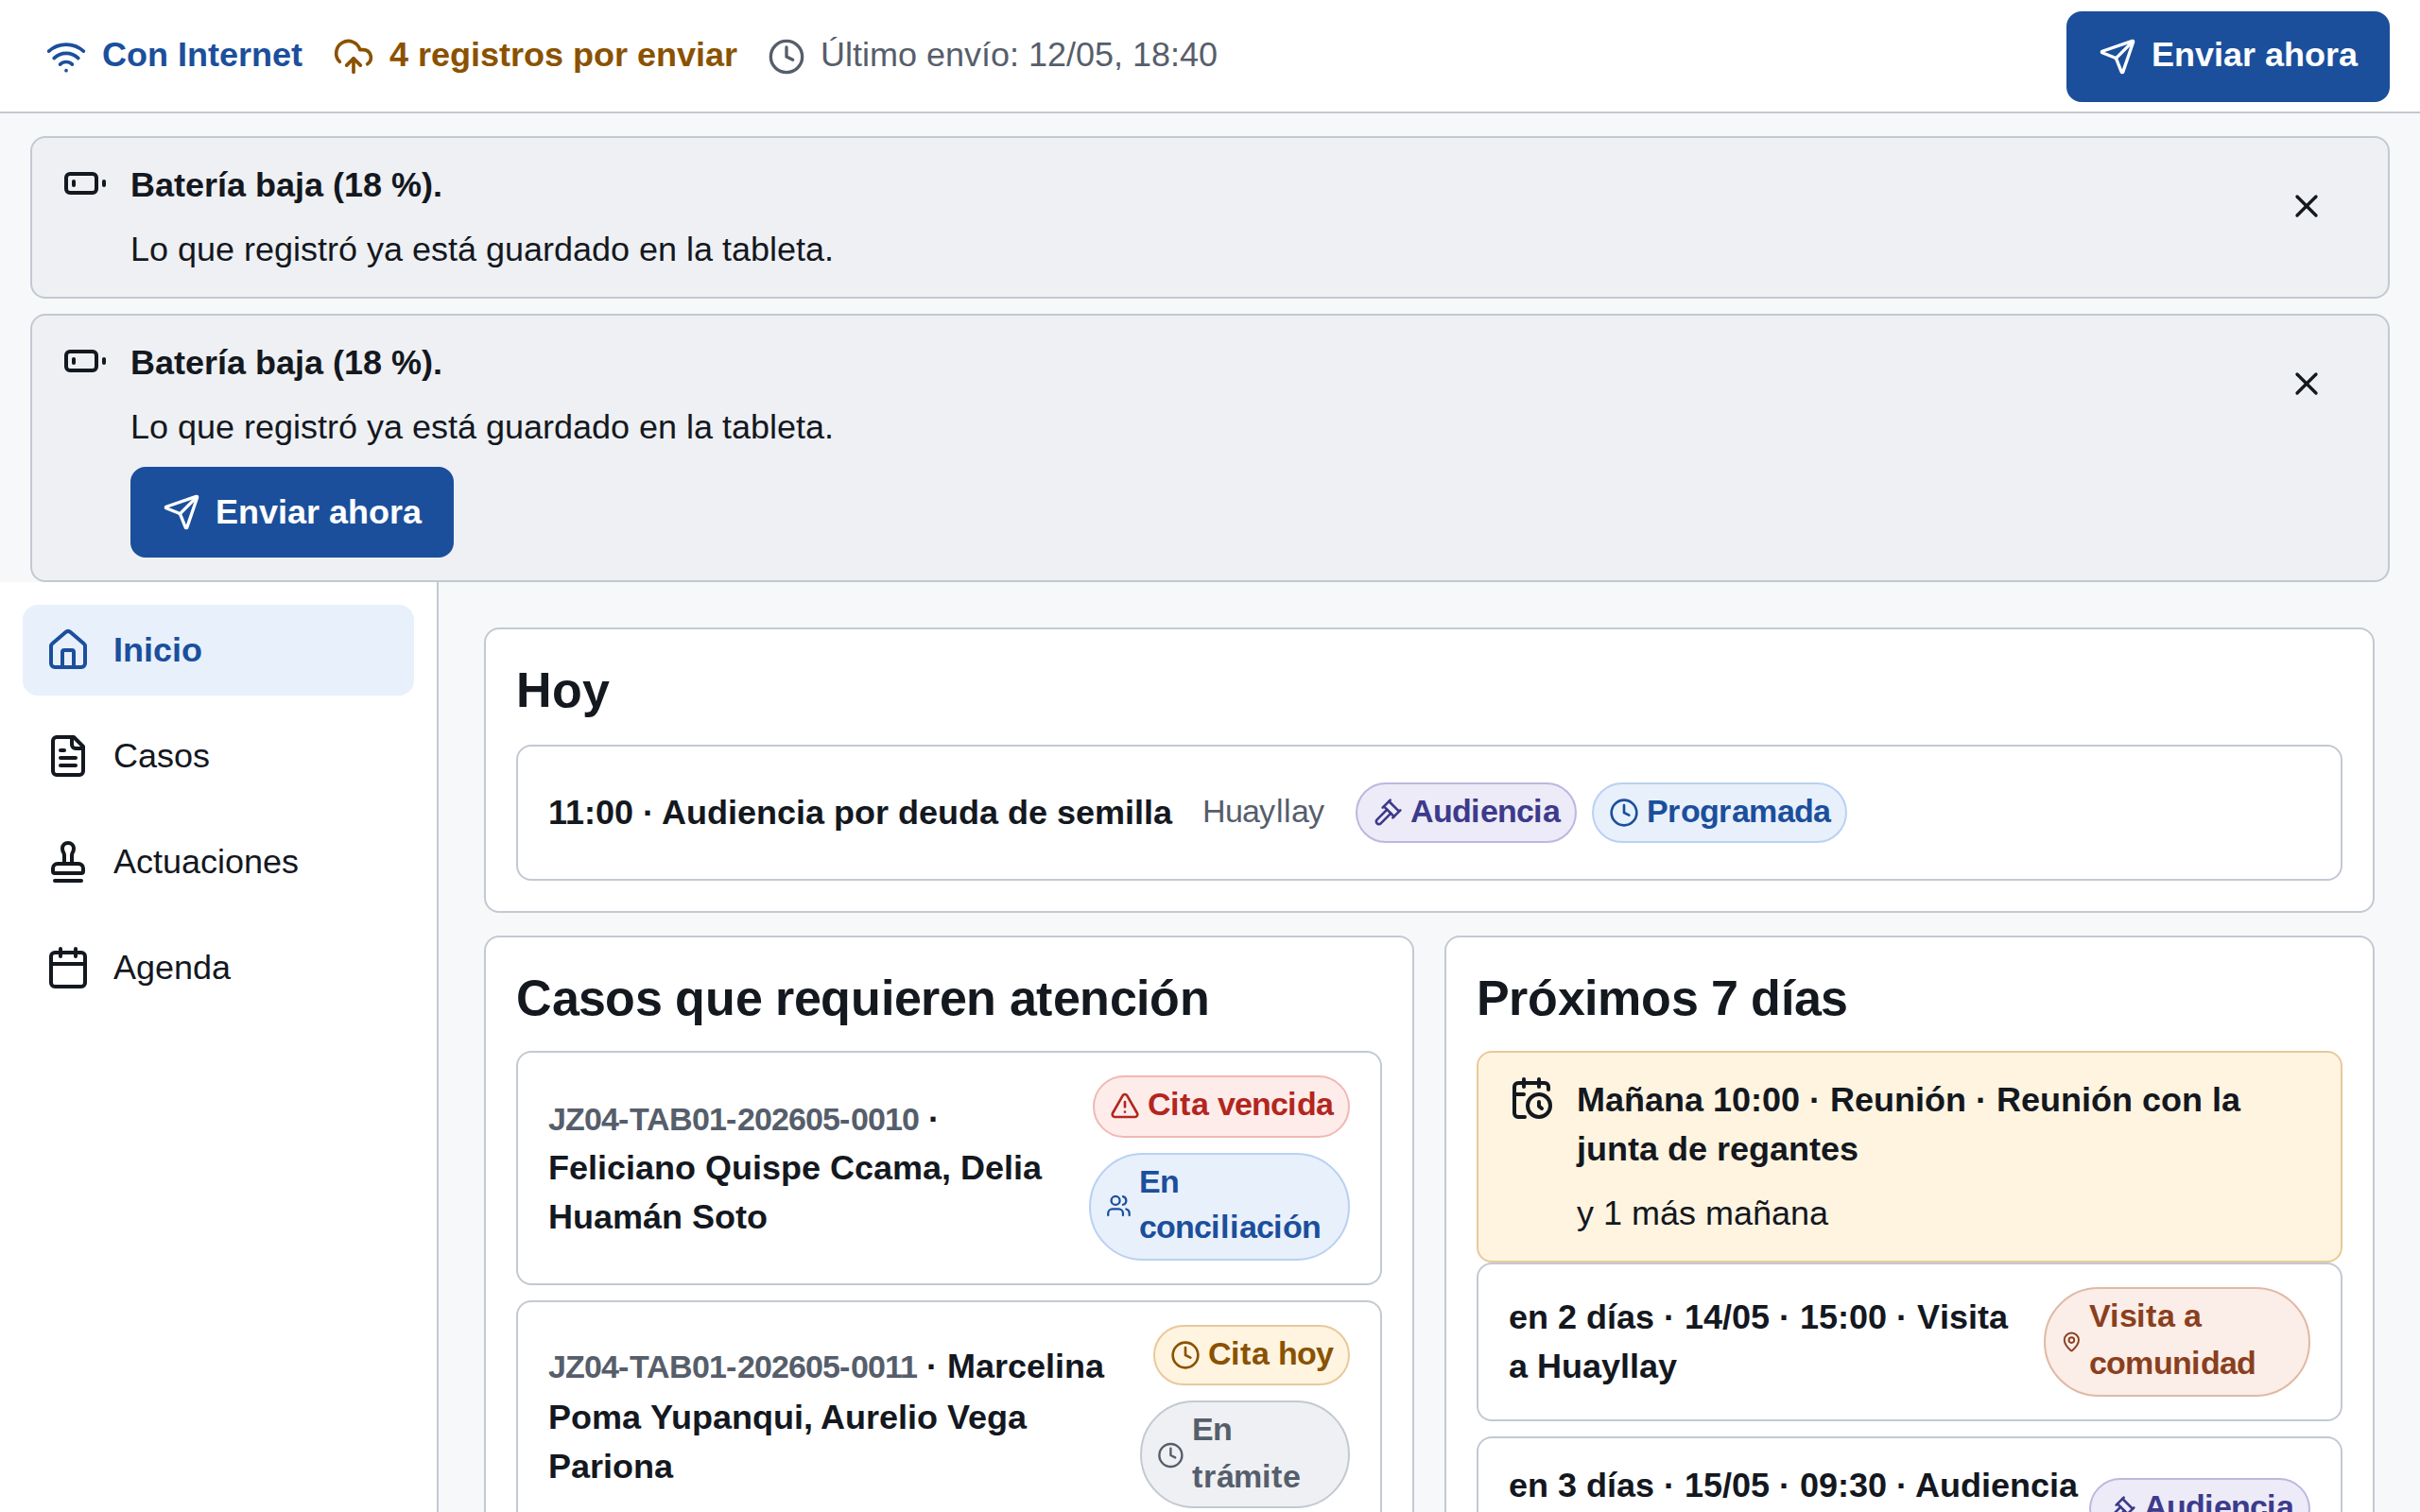
\includegraphics[width=0.78\linewidth]{capturas/X-02_bateria-20.png}
\caption{P-01 · Batería al 20 \%. Aviso de batería que recuerda que lo registrado ya está guardado}
\end{figure}
\begin{figure}[H]\centering
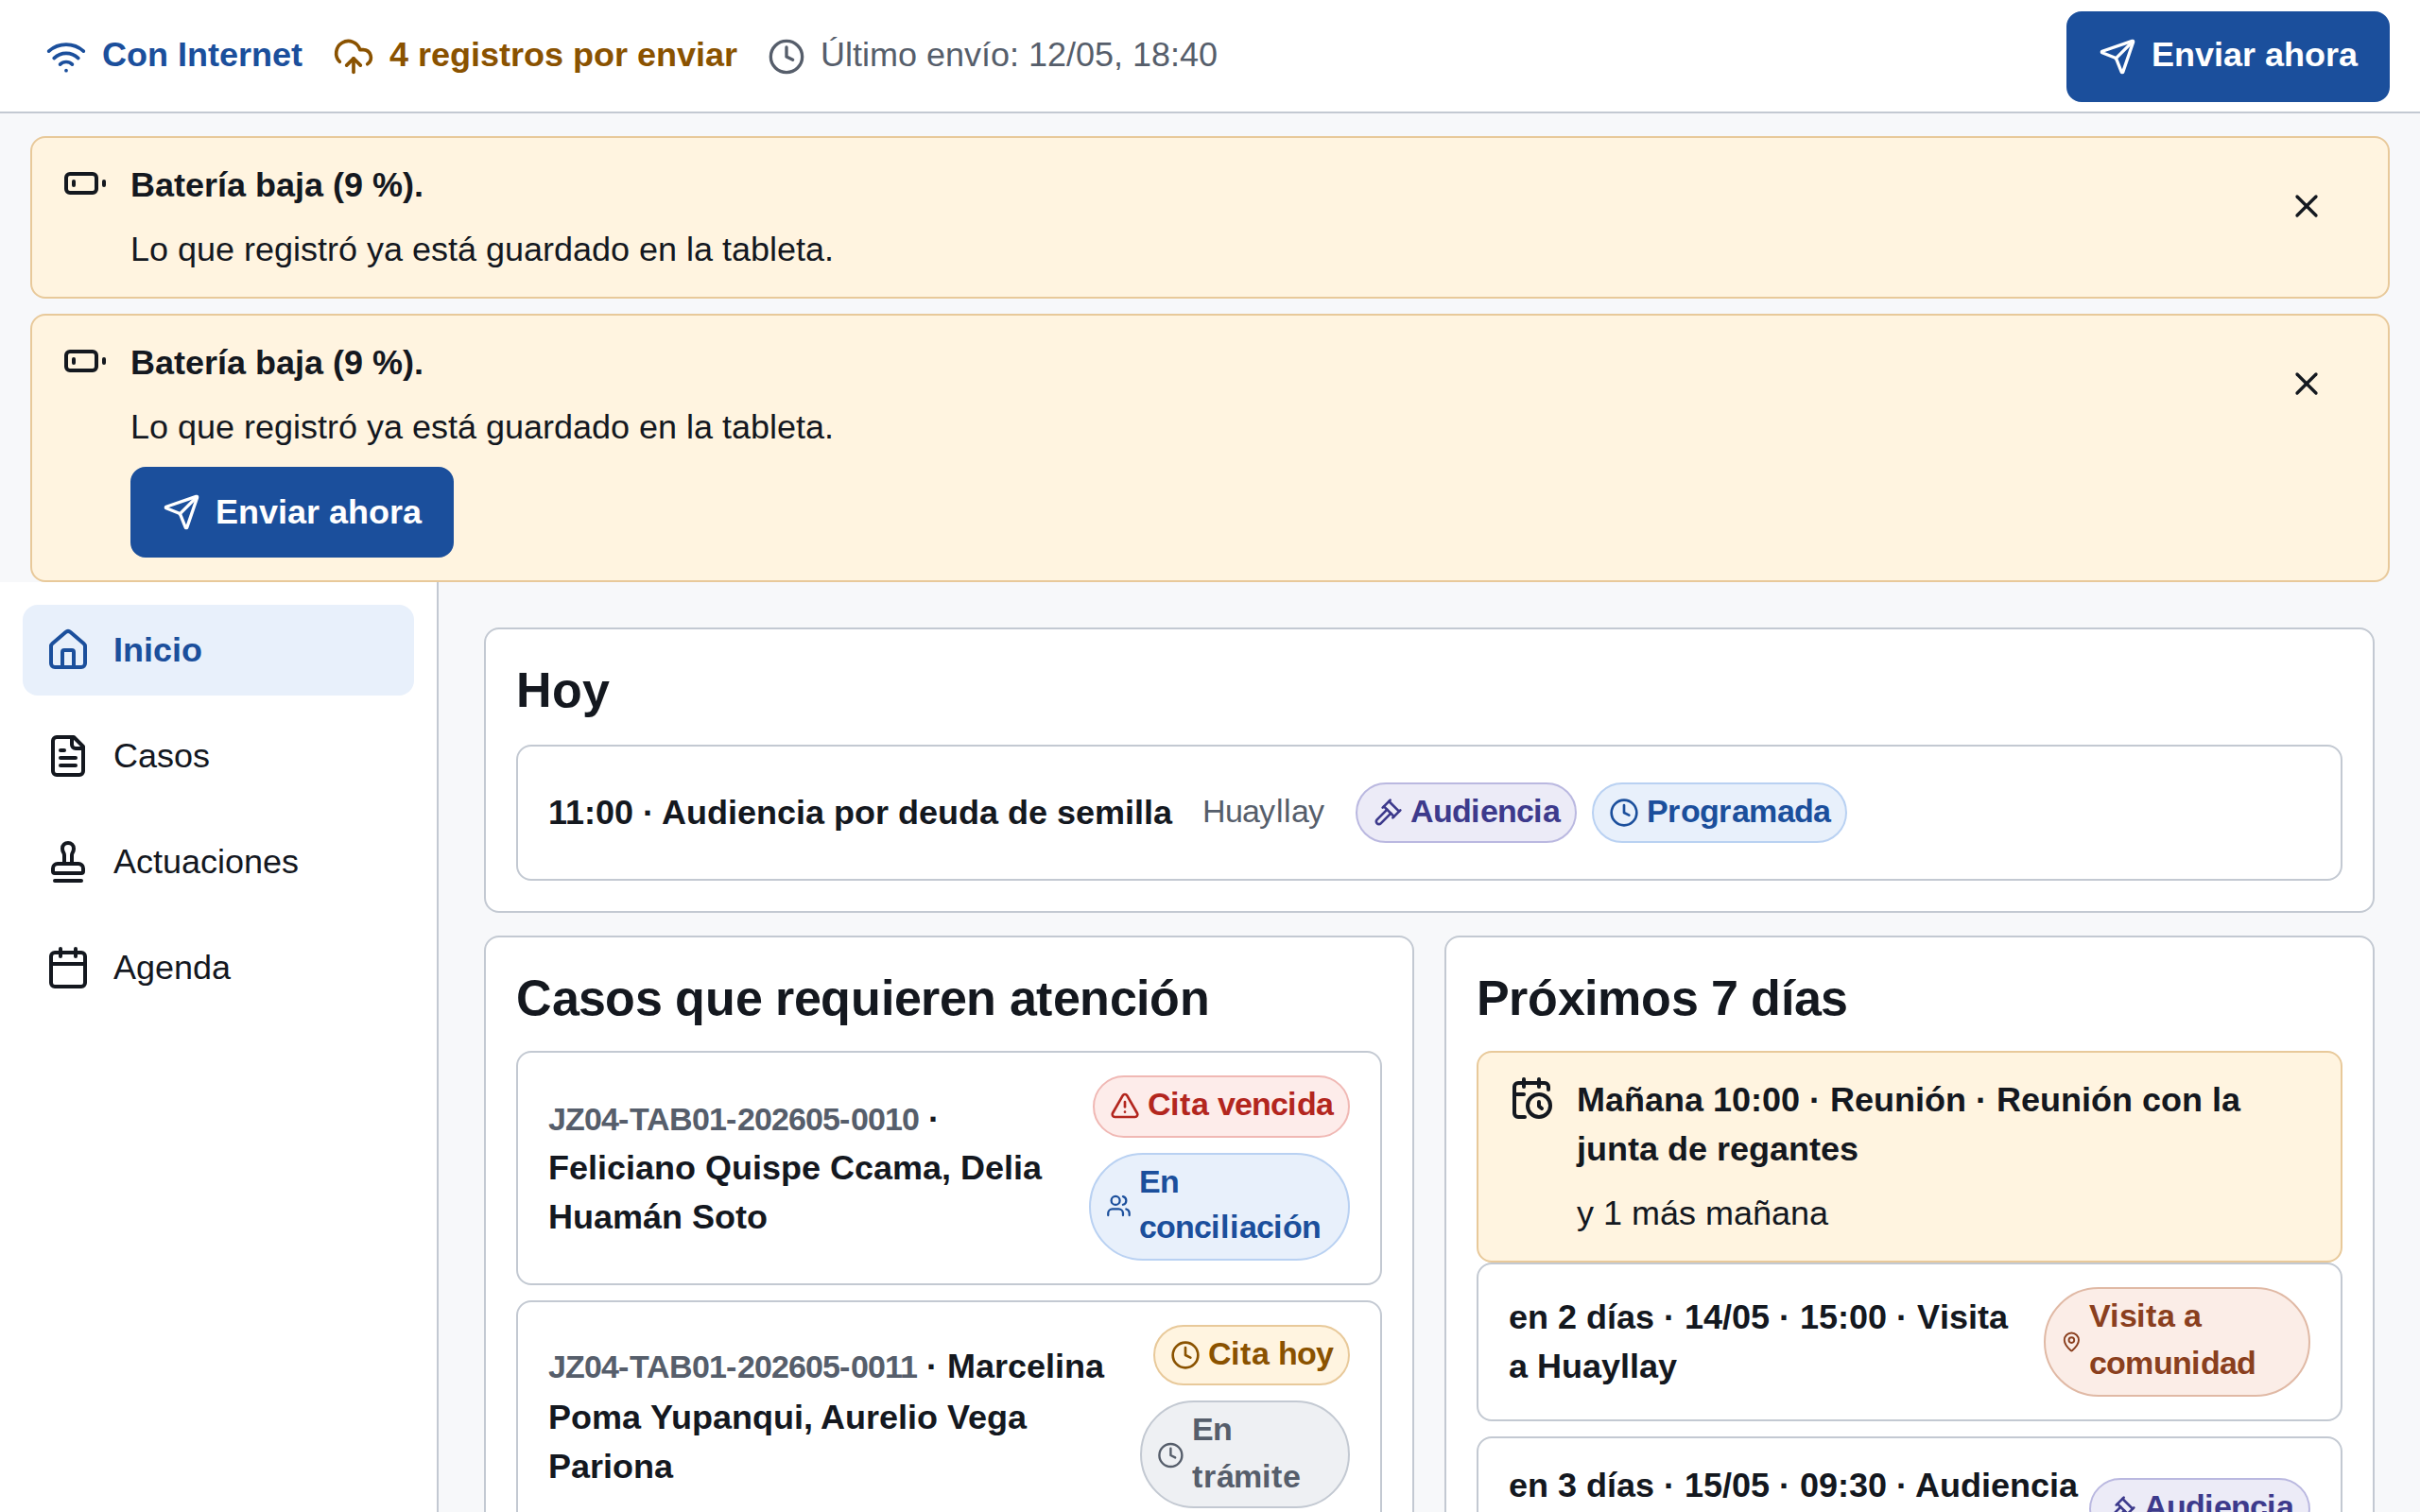
\includegraphics[width=0.78\linewidth]{capturas/X-03_bateria-10.png}
\caption{P-01 · Batería al 10 \%. El mismo aviso, más visible, con la opción de enviar si hay Internet}
\end{figure}
\begin{figure}[H]\centering
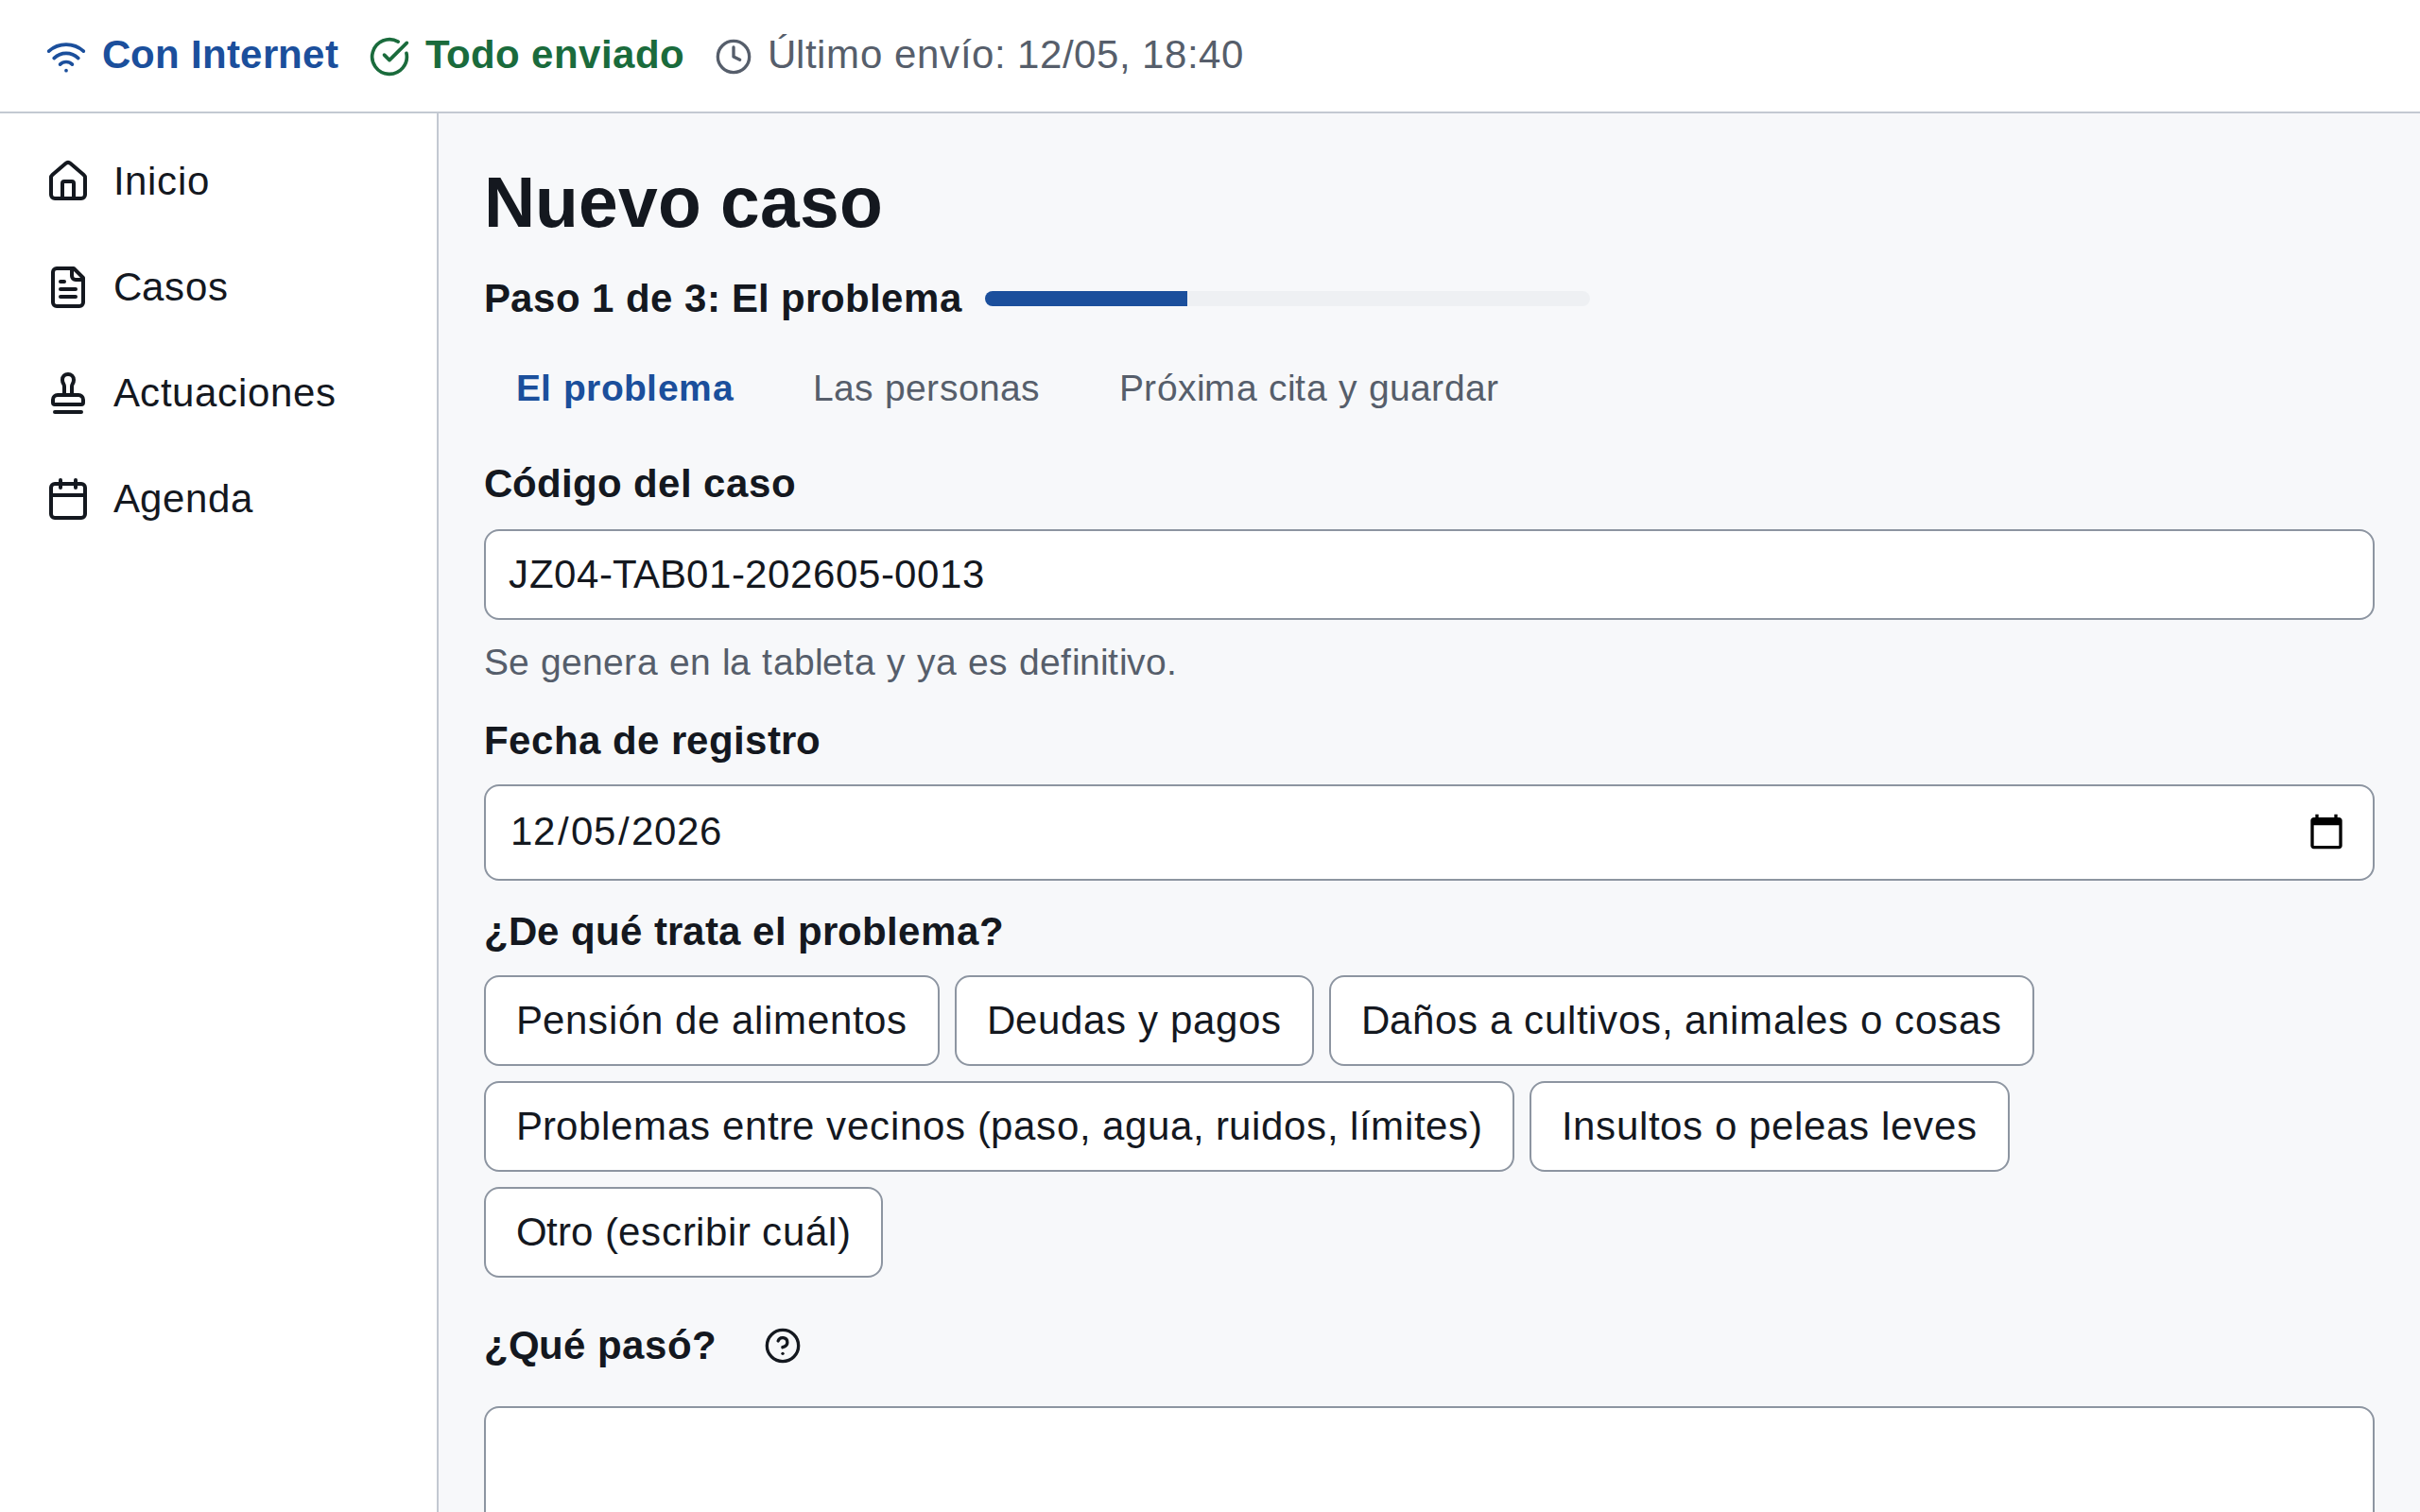
\includegraphics[width=0.78\linewidth]{capturas/X-04_letra-grande.png}
\caption{P-03 · Letra grande. El formulario no se rompe con la letra grande}
\end{figure}
\begin{figure}[H]\centering
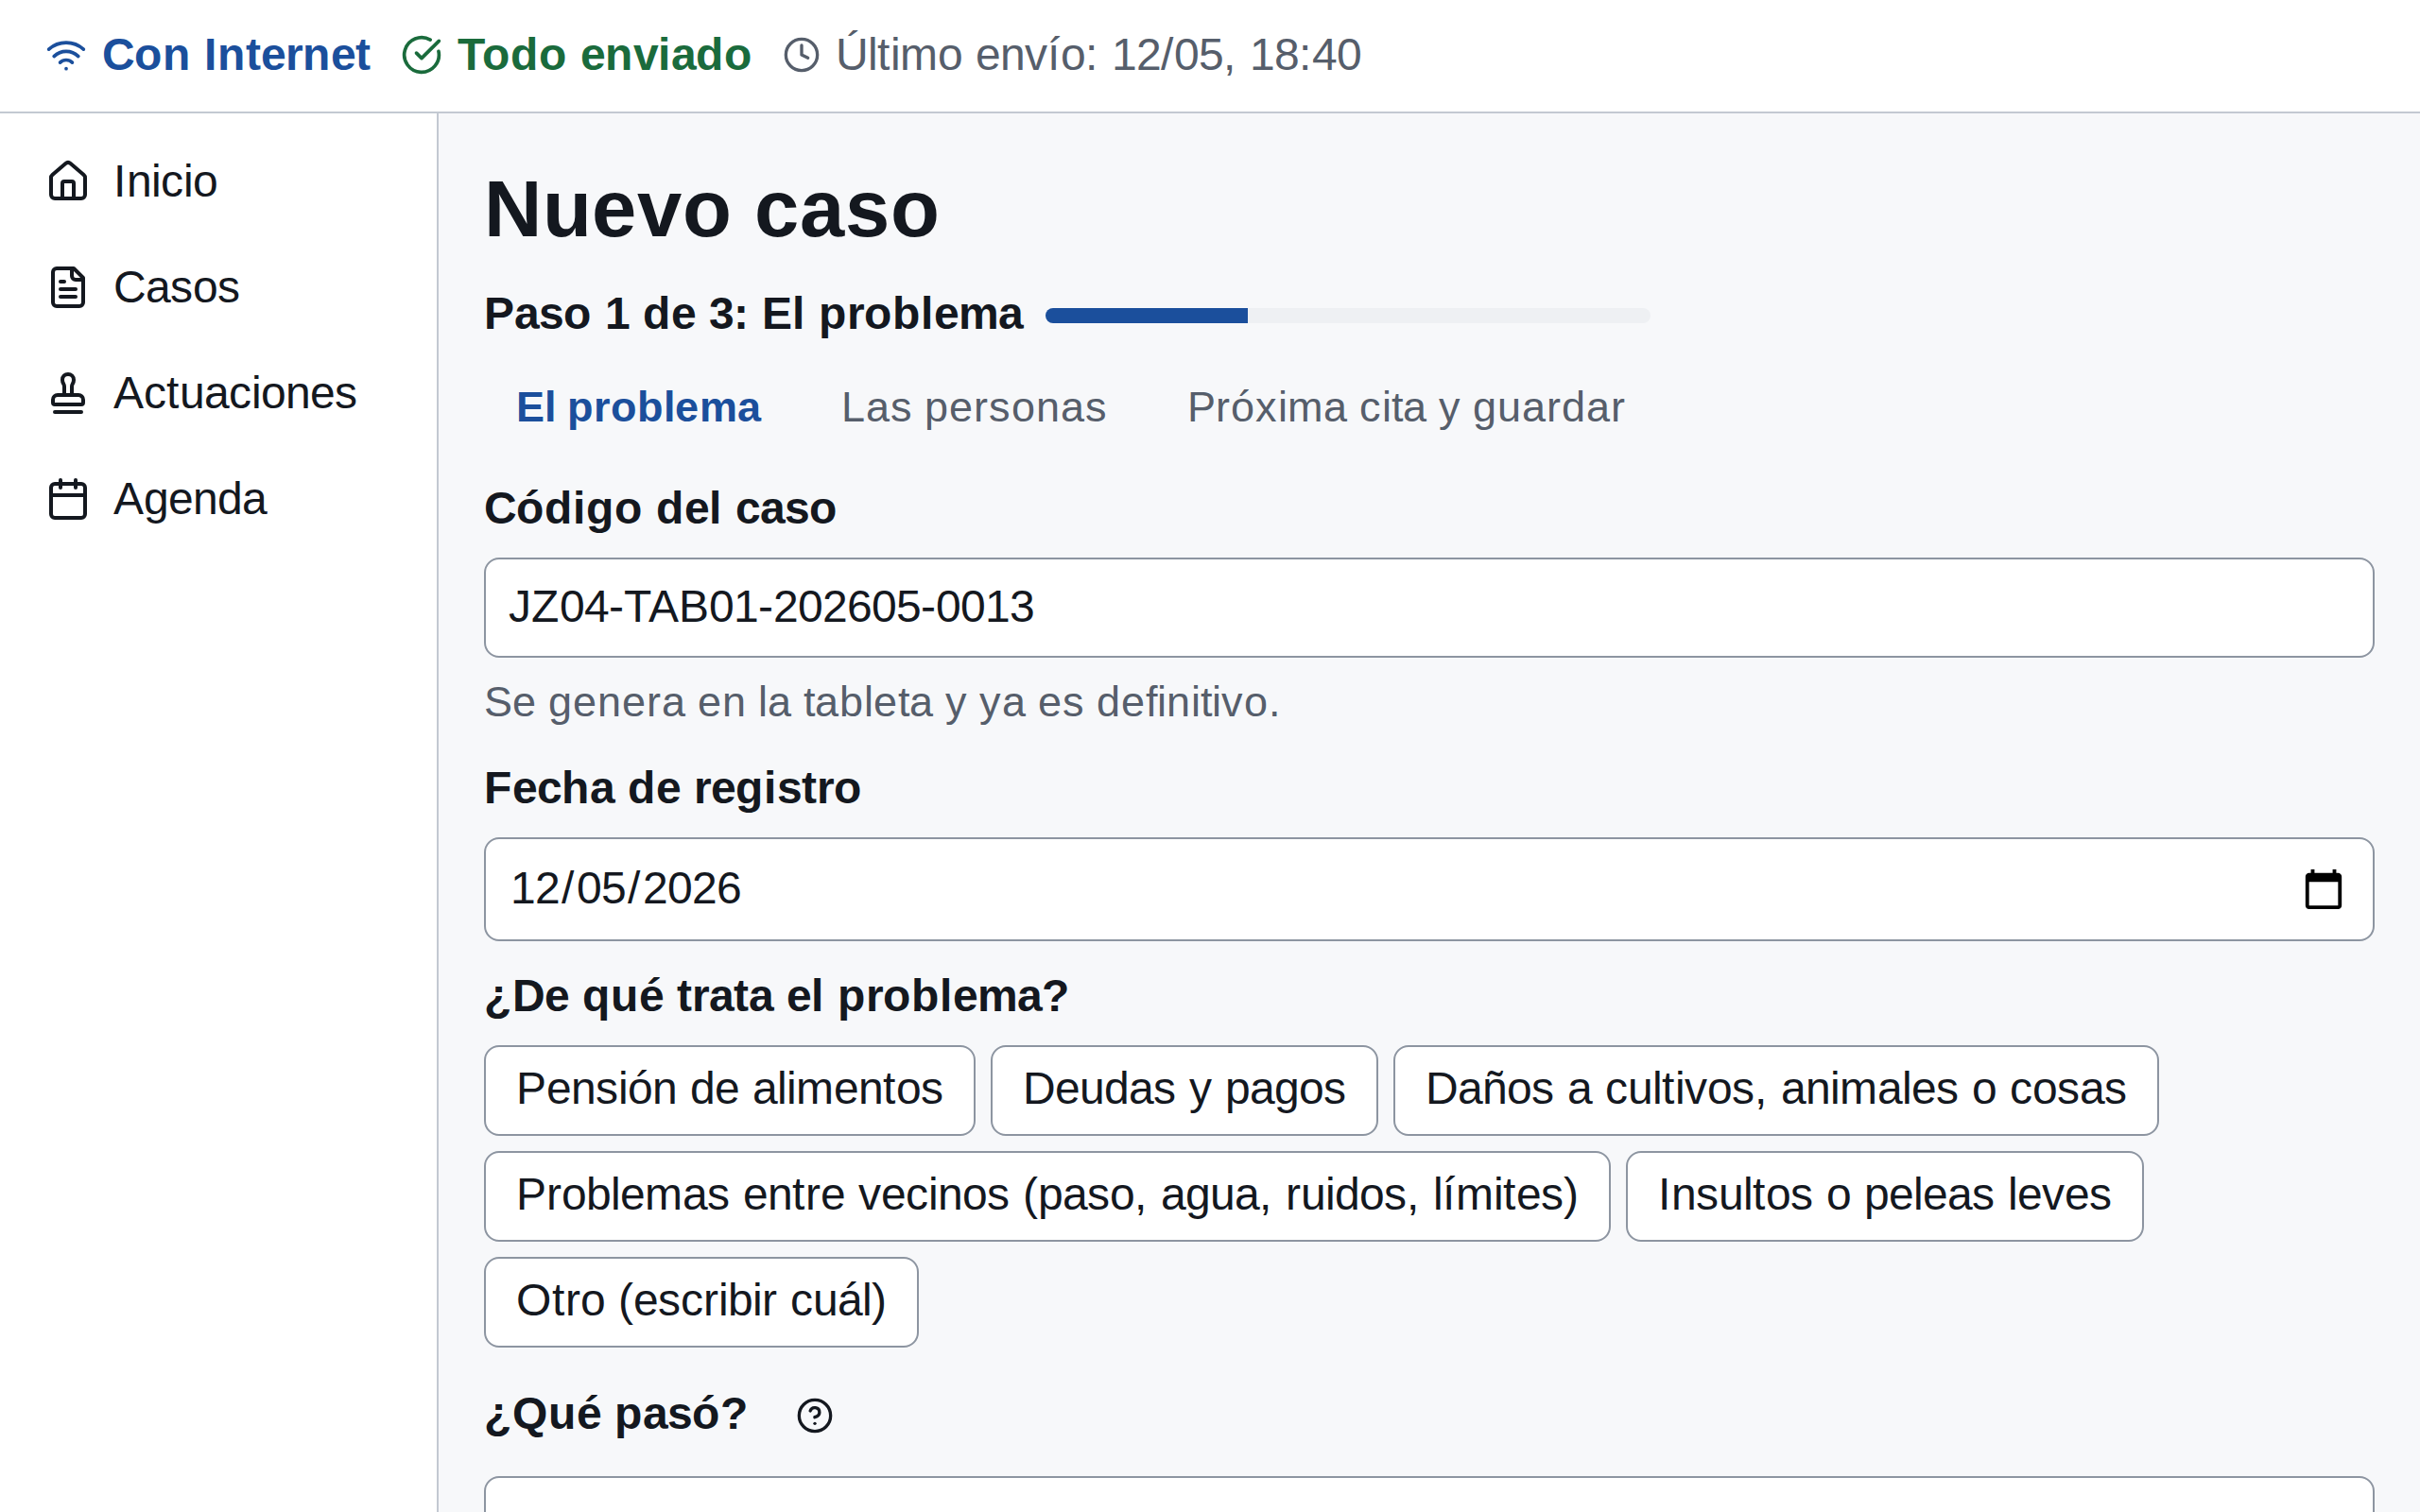
\includegraphics[width=0.78\linewidth]{capturas/X-05_letra-muy-grande.png}
\caption{P-03 · Letra muy grande. Sigue usándose con la letra muy grande, para presbicia}
\end{figure}
\begin{figure}[H]\centering
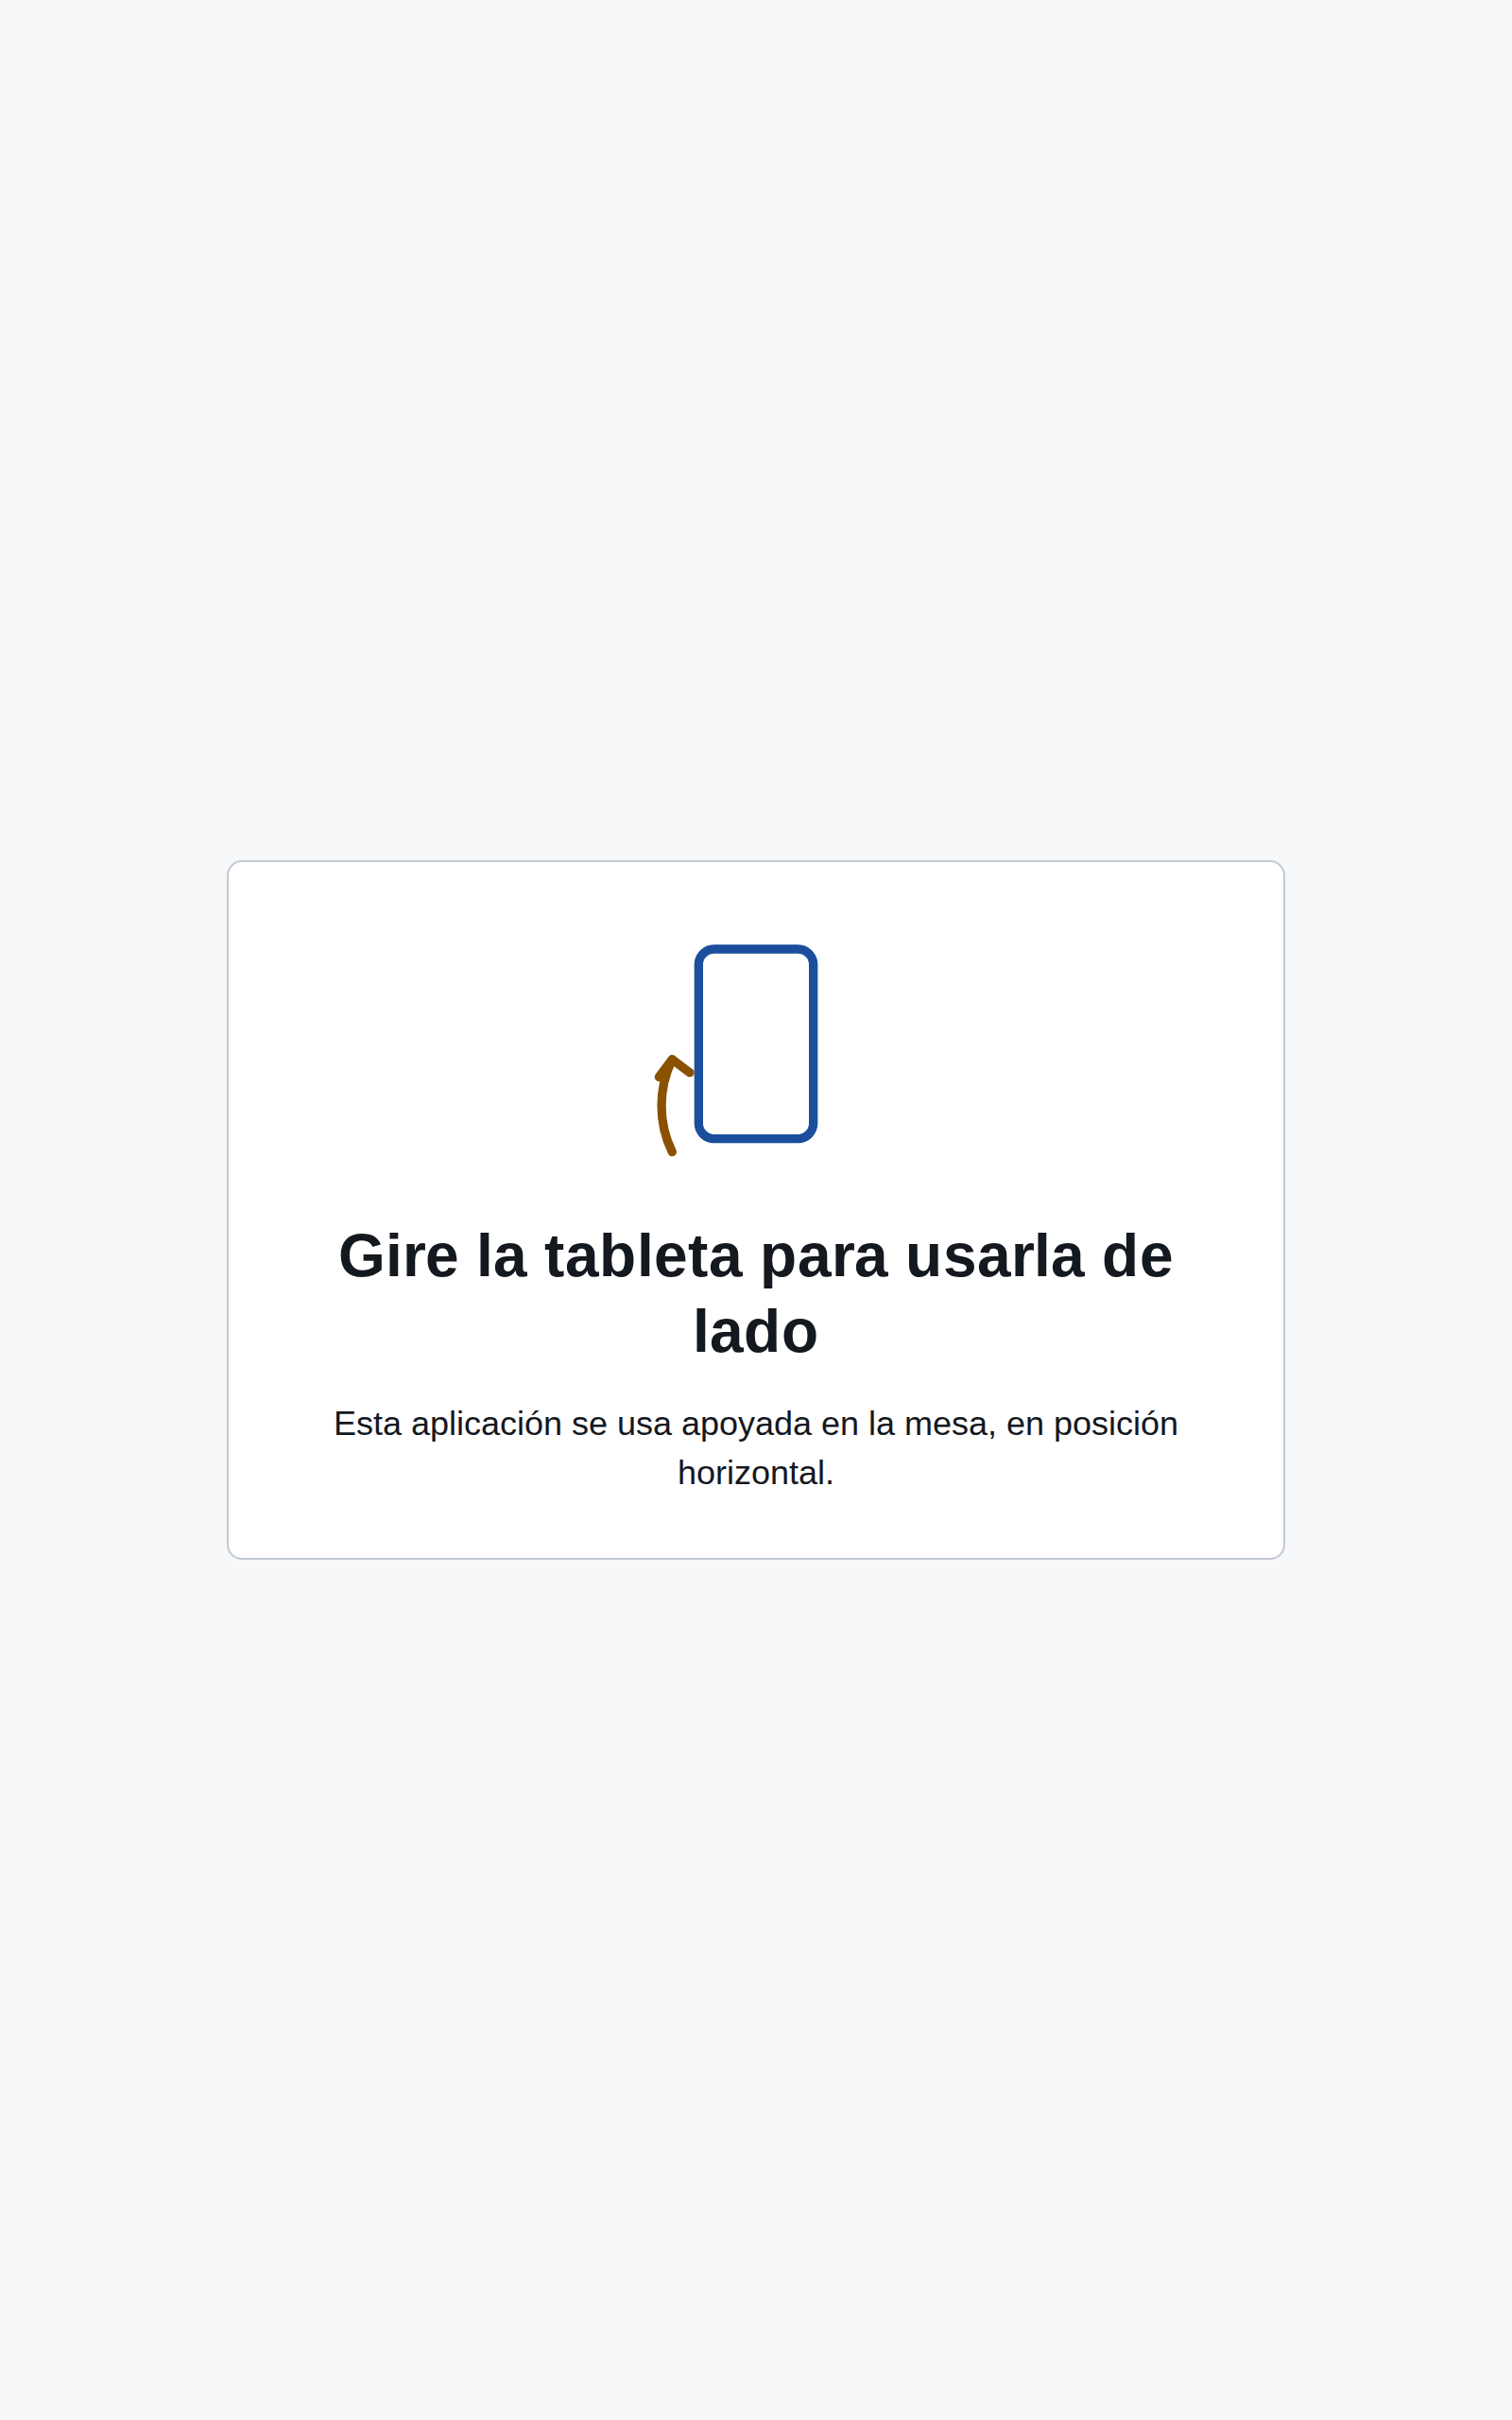
\includegraphics[width=0.78\linewidth]{capturas/X-06_orientacion.png}
\caption{Orientación · Tableta en vertical. Mensaje para girar la tableta, con ilustración, en vez de un diseño roto}
\end{figure}


\section{Matriz de justificación}

Los identificadores están agrupados por pantalla: del 1 al 8 los elementos transversales, del 10 al 19 casos, del 20 al 29 actuaciones, del 30 al 39 agenda, del 40 al 49 envío y computadora, del 50 al 55 el ingreso y la ayuda, del 60 al 66 el inicio. Los huecos entre bloques son deliberados: cada bloque queda reservado.

Cada fila es un elemento concreto de una pantalla, no un principio en abstracto. El número de cada fila coincide con el marcador numerado que aparece en las capturas anotadas de la sección siguiente.

\begin{landscape}
\footnotesize
\setlength{\tabcolsep}{4pt}
\begin{longtable}{@{}p{0.6cm}p{1.5cm}p{3.6cm}p{3.4cm}p{2.2cm}p{2.8cm}p{2.3cm}p{4.6cm}@{}}
\toprule
\textbf{ID} & \textbf{Pantalla} & \textbf{Elemento} & \textbf{Necesidad de la jueza} & \textbf{Principio de Norman} & \textbf{Heurística de Nielsen} & \textbf{Factor humano} & \textbf{Cómo facilita la interacción o previene errores} \\
\midrule
\endfirsthead
\toprule
\textbf{ID} & \textbf{Pantalla} & \textbf{Elemento} & \textbf{Necesidad de la jueza} & \textbf{Principio de Norman} & \textbf{Heurística de Nielsen} & \textbf{Factor humano} & \textbf{Cómo facilita la interacción o previene errores} \\
\midrule
\endhead
\bottomrule
\endfoot
1 & Todas & Indicador de conexión en la barra: ícono wifi o wifi tachado + texto «Con Internet» / «Sin Internet · puede seguir trabajando» & Trabaja en comunidades donde la señal va y viene y necesita saber si está conectada sin interpretarlo & Feedback & H1 Visibilidad del estado del sistema & Poca experiencia digital; legibilidad al aire libre & El estado se lee en texto y no solo por color; «Sin Internet» va en gris y no en rojo, así no interpreta como avería lo que en campo es lo normal, y no interrumpe el registro por creer que algo falló \\
2 & Todas & Contador «N registros por enviar» / «Todo enviado» con ícono de nube & Saber cuánto trabajo suyo todavía existe solo en la tableta & Feedback; modelo conceptual & H1 Visibilidad del estado & Carga de memoria de trabajo & Sustituye el recuerdo por un número siempre visible; evita que dé por enviado lo que no salió y que pierda registros si la tableta se daña \\
3 & Todas & Botón [Enviar ahora] visible en la barra cuando hay pendientes y hay Internet & Enviar en cuanto aparece señal, sin buscar dónde & Affordance; signifier & H7 Flexibilidad y eficiencia & Ley de Fitts (objetivo grande y fijo) & La acción aparece solo cuando es posible y en un lugar fijo; evita tocar un botón que no haría nada y evita depender de descubrir que la barra se puede tocar \\
4 & Todas & Menú lateral fijo de 4 opciones con ícono + texto & Moverse entre casos, trámites y agenda sin aprender rutas & Mapping; modelo conceptual & H4 Consistencia; H6 Reconocer antes que recordar & Ley de Hick (4 opciones); tableta de 10 pulgadas apoyada en mesa & Cuatro destinos siempre en el mismo sitio reducen el tiempo de decisión y evitan que se pierda dentro de la aplicación \\
5 & P-02, P-05, P-07 & Un solo campo de búsqueda que acepta nombre, DNI o código & Buscar por lo que recuerda de la persona, no por el campo correcto & Constraints & H6 Reconocer antes que recordar & Poca experiencia digital & No obliga a elegir antes en qué campo buscar; evita el error de escribir el dato correcto en el buscador equivocado y no encontrar nada \\
6 & P-02, P-05, P-07 & Filtros como botones visibles (comunidad, estado, tipo, fechas) y no como listas desplegables & Acotar una lista larga con un toque, sin teclear & Signifier & H6 Reconocer antes que recordar; H8 Minimalismo & Ley de Fitts; interacción táctil & Las opciones se ven todas a la vez y se activan con un toque; evita el desplegable, que en táctil es un objetivo pequeño y esconde las opciones \\
7 & P-03, P-06, P-08 & Etiqueta «(opcional)» en texto junto al campo, sin asteriscos & No conoce la convención del asterisco y duda si puede dejar un campo vacío & Signifier & H2 Lenguaje del mundo real; H6 Reconocer antes que recordar & Poca experiencia digital & Continúa sin el dato sin temer que el registro no se guarde; evita que invente un teléfono o un DNI solo para «llenar» el campo \\
8 & P-03, P-06 & Botón [Agregar persona] que abre una ventana con los datos de una sola persona & Registrar varias partes sin confundir de quién es cada dato & Constraints & H5 Prevención de errores; H8 Minimalismo & Carga de lectura & Aísla los datos de cada persona en una sola pantalla; evita mezclar el DNI de una parte con el nombre de otra en un formulario largo \\
10 & P-02 & Lista ordenada poniendo primero los casos que requieren atención & Saber por dónde empezar el día sin revisar caso por caso & Mapping & H1 Visibilidad del estado; H8 Minimalismo & Carga de lectura & Pone arriba lo que vence; evita que una cita vencida quede enterrada al final de la lista y se pase por alto \\
11 & P-02, P-01 & Marca con el motivo de atención en texto: «Cita vencida», «Cita hoy», «22 días sin avance» & Entender por qué un caso pide atención, no solo que la pide & Feedback & H1 Visibilidad del estado; H2 Lenguaje del mundo real & Poca experiencia digital; legibilidad al aire libre & El motivo va escrito con ícono, no codificado en un color; evita que confunda urgencias distintas y le dice qué hacer a continuación \\
12 & P-03 & Campo «Código» de solo lectura, generado en la tableta & Identificar el caso sin depender de conexión ni de inventar una numeración & Constraints & H5 Prevención de errores & Poca experiencia digital & El código no se puede escribir mal ni repetir; el prefijo de tableta evita que choque con los que crea la computadora \\
13 & P-03, P-06 & Indicador «Paso 2 de 3» con barra de avance y los tres títulos & Llenar un formulario largo sin perder de vista cuánto falta & Feedback; modelo conceptual & H1 Visibilidad del estado; H3 Control y libertad & Carga de memoria de trabajo & Divide la tarea en tres tramos cortos y deja volver atrás; evita el abandono a mitad y el error por cansancio en un formulario de una sola pantalla \\
14 & P-03 & Tarjeta «Revise antes de guardar» con el caso escrito en frases completas & Confirmar los datos con las partes, que están delante de ella & Feedback & H5 Prevención de errores; H9 Reconocer y recuperarse de errores & Pantalla que la jueza muestra a los ciudadanos & Permite leer el registro en voz alta antes de guardarlo; corrige nombres y comunidades mal anotados mientras las personas siguen presentes \\
15 & P-03 & Botón [Guardar y salir] disponible en los pasos 1 y 2 & Interrumpirse cuando llega otra persona, sin perder lo escrito & Affordance & H3 Control y libertad; H7 Flexibilidad & Trabajo interrumpido en campo & Lo guardado queda como Borrador en vez de perderse; evita que tenga que terminar un caso a la fuerza para no perder veinte minutos de trabajo \\
16 & P-04 & Acciones [Editar datos] y [Registrar avance] siempre abajo a la derecha & Encontrar la acción principal en el mismo sitio en toda la aplicación & Mapping; signifier & H4 Consistencia y estándares & Ley de Fitts; tableta apoyada en mesa & La acción aparece donde termina el recorrido de lectura y no cambia de lugar entre pantallas; evita buscarla y evita tocar la equivocada \\
17 & P-04 & Campo modificado con borde azul y la marca «Modificado» & Ver qué cambió antes de confirmar una edición & Feedback & H1 Visibilidad del estado; H5 Prevención de errores & Interacción táctil & Señala el cambio en el momento; evita guardar una modificación hecha por accidente al apoyar la mano en la pantalla \\
18 & P-04 & Botón [Deshacer cambios] & Volver atrás sin miedo a haber estropeado un expediente & Affordance & H3 Control y libertad; H9 Recuperarse de errores & Poca experiencia digital & Restaura los valores originales con un toque; reduce el miedo a tocar y permite explorar la edición sin consecuencias \\
19 & P-04 & Campo condicional «Acuerdo o resultado» con la línea «Se pide cuando el caso pasa a Concluido» & Cerrar un caso dejando constancia de en qué quedó & Constraints & H5 Prevención de errores; H2 Lenguaje del mundo real & Poca experiencia digital & El campo aparece solo cuando corresponde y explica por qué se pide; evita cerrar casos vacíos que después nadie puede reconstruir \\
20 & P-06 & Catálogo de trámites en tarjetas con etiqueta cotidiana y descripción & Elegir el trámite por lo que la persona le pidió, no por su nombre legal & Signifier; modelo conceptual & H2 Lenguaje del mundo real; H6 Reconocer antes que recordar & Ley de Hick; carga de lectura & Reconoce el trámite en vez de recordar su nombre; evita elegir mal el tipo por confundir dos términos legales parecidos \\
21 & P-06 & Solo 4 tarjetas visibles y botón [Ver más trámites] & Encontrar rápido los trámites que pide casi todo el mundo & Constraints & H8 Minimalismo; H7 Flexibilidad & Ley de Hick aplicada a la carga de lectura, no solo al número de opciones & Reduce a cuatro la lectura inicial y deja el resto a un toque; evita recorrer ocho descripciones largas para el caso más común \\
22 & P-06 & Término legal en gris debajo de la etiqueta cotidiana («Legalización de firma») & Usar el nombre legal cuando el documento lo exige, sin tener que saberlo de memoria & Mapping & H2 Lenguaje del mundo real; H10 Ayuda y documentación & Poca experiencia digital; vocabulario jurídico & Presenta los dos nombres juntos y jerarquizados; evita que elija por el término legal creyendo que es otro trámite \\
23 & P-06 & Estado de atención en botones segmentados con su definición escrita debajo & Distinguir «lo pidió», «ya se atendió» y «ya se entregó» & Feedback; constraints & H2 Lenguaje del mundo real; H5 Prevención de errores & Carga de lectura; vocabulario jurídico frente al cotidiano & La definición está a la vista al elegir; evita marcar Concluida cuando el documento todavía no se entregó \\
24 & P-06 & Encabezado con dos estados separados: «Estado del registro: Borrador · falta: …» y «Estado de atención» & Saber si al trámite le faltan datos, aparte de en qué punto va la atención & Modelo conceptual & H1 Visibilidad del estado; H4 Consistencia & Carga de lectura & Dice exactamente qué falta y no mezcla las dos ideas; evita creer que un trámite está completo porque está marcado como Atendida \\
25 & P-06 & Campo condicional «Fecha de atención» con la línea «Se pide desde que el trámite está Atendida» & Registrar cuándo se atendió sin que el formulario pida datos que aún no existen & Constraints & H5 Prevención de errores; H8 Minimalismo & Poca experiencia digital & El campo aparece cuando tiene sentido y valida que no sea anterior a la solicitud; evita fechas imposibles en el expediente \\
26 & P-06 & Aviso de trámite parecido con [Es el mismo: abrirlo] y [Es otro: continuar] & No abrir dos veces el mismo trámite cuando la persona vuelve a preguntar & Feedback & H5 Prevención de errores; H3 Control y libertad & Carga de memoria de trabajo & Advierte mostrando el registro parecido, pero nunca bloquea; evita duplicados sin impedir registrar dos trámites legítimamente parecidos \\
27 & P-06 & Botón [Guardar como borrador] en los pasos 1 y 2 & Guardar lo que ya sabe aunque falte información que la persona traerá después & Affordance & H3 Control y libertad; H7 Flexibilidad & Trabajo interrumpido; atención por orden de llegada & Permite guardar incompleto de forma explícita; evita la disyuntiva entre inventar un dato o perder lo escrito \\
28 & P-05 & Bloque de búsqueda con filtros combinables y casilla «Mostrar solo borradores» & Encontrar los trámites a medio terminar para cerrarlos & Signifier & H6 Reconocer antes que recordar; H7 Flexibilidad & Carga de memoria de trabajo & Convierte «qué me falta terminar» en un filtro de un toque; evita repasar la lista entera de memoria \\
29 & P-05 & Tres marcas por fila: estado de atención, borrador con lo que falta, y si ya se envió & Juzgar una fila sin abrirla & Feedback & H1 Visibilidad del estado; H4 Consistencia & Legibilidad al aire libre & Cada marca lleva ícono y texto, nunca solo color; evita abrir trámites uno por uno para saber en qué van \\
30 & P-07 & Selector [Mes] [Semana] [Día] en botones grandes segmentados & Mirar la carga del mes o el detalle del día según lo que esté decidiendo & Mapping & H7 Flexibilidad; H3 Control y libertad & Ley de Fitts; tableta de 10 pulgadas & Cambiar de nivel de detalle cuesta un toque y conserva el día y los filtros; evita perder el contexto al cambiar de vista \\
31 & P-07, P-01 & Franja «Mañana: 2 actividades» con título y hora & Preparar lo de mañana antes de cerrar la tableta & Feedback & H1 Visibilidad del estado; H6 Reconocer antes que recordar & Carga de memoria de trabajo & Trae lo inmediato sin que tenga que ir a buscarlo; evita llegar a una audiencia sin haber avisado a las partes \\
32 & P-07 & Tarjeta de actividad con borde de color, ícono de categoría y estado en texto & Reconocer de un vistazo qué tipo de actividad es y si ya ocurrió & Signifier; mapping & H4 Consistencia; H1 Visibilidad del estado & Legibilidad al aire libre; visión del color & El color acompaña al ícono y al texto, nunca los sustituye; sigue siendo legible con sol y para quien no distingue bien los colores \\
33 & P-07 & Vista mes con hasta 3 actividades por día y «+N más» & Ver la carga del mes sin perder la cuenta de lo que no cabe & Feedback & H1 Visibilidad del estado; H8 Minimalismo & Pantalla de 10 pulgadas; carga de lectura & Dice cuántas quedan fuera en vez de esconderlas; evita planificar un viaje creyendo que ese día está libre \\
34 & P-07 & Línea «Creada desde el caso JZ04-…» que lleva al expediente & Volver del compromiso de agenda al caso que lo originó & Mapping; modelo conceptual & H4 Consistencia; H7 Flexibilidad & Teclado en pantalla & Une agenda y expediente con un toque; evita copiar el código a mano y buscarlo en la otra sección \\
35 & P-08 & Categoría de la actividad en botones grandes con ícono & Clasificar la actividad sin escribir & Signifier & H6 Reconocer antes que recordar; H5 Prevención de errores & Ley de Fitts; interacción táctil & Cuatro opciones fijas evitan el tecleo y los nombres inventados; sin categoría no queda Completa, y el mensaje lo dice \\
36 & P-08 & Campo condicional «Hora de término» con la línea «Se pide cuando puso una hora de inicio» & Registrar cuánto dura una audiencia solo cuando tiene hora & Constraints & H5 Prevención de errores; H8 Minimalismo & Poca experiencia digital & El campo aparece solo cuando aplica y valida que termine después de empezar; evita rangos horarios imposibles \\
37 & P-08 & Aviso «A esa hora ya tiene: Visita a Huayllay» con [Agendar igual] & No comprometerse dos veces a la misma hora en comunidades distintas & Feedback & H5 Prevención de errores; H3 Control y libertad & Carga de memoria de trabajo; distancias entre comunidades & Muestra con qué choca antes de guardar y deja decidir; evita el doble compromiso sin impedir los solapamientos intencionales \\
38 & P-08 & Aviso no bloqueante de fecha pasada: «Está agendando en una fecha que ya pasó» & Registrar también lo que ya ocurrió, sin que el sistema lo trate como error & Feedback & H5 Prevención de errores; H9 Recuperarse de errores & Reloj de la tableta desfasado sin conexión & Pregunta en vez de bloquear; detecta el año mal escrito pero permite registrar una actividad atrasada \\
39 & P-08 & Recordatorio en tres botones, prellenado en «1 día antes» & Que la aplicación le avise sin tener que configurarlo cada vez & Constraints & H7 Flexibilidad; H8 Minimalismo & Poca experiencia digital & El valor por defecto cubre el caso normal y se cambia con un toque; evita agendar sin aviso por olvidar configurarlo \\
40 & P-09 & Lista de los registros por enviar con su marca «En la tableta» y el botón [Enviar ahora] & Ver exactamente qué es lo que todavía no salió & Feedback; modelo conceptual & H1 Visibilidad del estado & Carga de memoria de trabajo & Convierte un número abstracto en una lista de registros con nombre; evita enviar creyendo que era otra cosa lo pendiente \\
41 & P-09 & Barra de progreso con «Enviando 2 de 4…» y el estado de cada registro & Saber que el envío avanza y no se quedó colgado & Feedback & H1 Visibilidad del estado & Conexiones lentas e intermitentes & Muestra avance real por registro; evita que cierre la aplicación a la mitad o que repita el envío por creer que no pasó nada \\
42 & P-09 & Aviso de resultado que siempre dice dónde quedaron los registros & Confiar en que su trabajo no se perdió, pase lo que pase & Feedback & H1 Visibilidad del estado; H9 Recuperarse de errores & Ansiedad por pérdida de datos & Cada desenlace nombra cuántos llegaron y dice que el resto sigue seguro en la tableta; evita el reenvío ansioso y la anotación duplicada en papel \\
43 & P-09 & Conflicto resuelto automáticamente con el cambio más reciente y aviso de qué campo se usó & Reducir trámites mientras las partes esperan y no dominar comparaciones complejas & Feedback & H1 Visibilidad del estado; H3 Control y libertad & Poca experiencia digital & Evita una decisión campo por campo propensa a errores y deja la opción de revertir; el envío no se detiene por una diferencia de texto \\
44 & P-09 & Comparación por campo en [Ver y cambiar], con las dos versiones y [Usar esta] & Recuperar su versión cuando la de la computadora estaba equivocada & Mapping & H3 Control y libertad; H9 Recuperarse de errores & Poca experiencia digital & La comparación existe pero es opcional; permite corregir una resolución automática sin obligar a revisarlas todas \\
45 & P-09 & Botón [Reintentar] tras un corte o un error del servidor & Volver a intentar sin rehacer nada & Affordance & H9 Recuperarse de errores; H3 Control y libertad & Conexiones intermitentes & El reintento es un toque sobre lo que quedó pendiente; evita volver a capturar registros que ya estaban guardados \\
46 & P-09 & Aviso gris «Sin Internet» con el botón de enviar deshabilitado & Entender por qué no puede enviar ahora mismo & Constraints; signifier & H1 Visibilidad del estado; H5 Prevención de errores & Poca experiencia digital & Explica la causa en vez de fallar al tocar; el gris y el texto «Se enviarán solos en cuanto haya Internet» quitan la sensación de avería \\
47 & P-10 & Aviso «La tableta envió datos por última vez el 12/05, 18:40» & Que quien consulta desde la sede no dé por completa una información parcial & Feedback & H1 Visibilidad del estado & Modelo mental compartido entre dos dispositivos & Marca el límite de lo que la computadora puede saber y nunca afirma cuántos registros quedan pendientes; evita decisiones tomadas sobre datos incompletos \\
48 & P-10 & Tablas anchas con más columnas y las mismas marcas de estado que la tableta & Revisar muchos expedientes de golpe desde una pantalla grande & Mapping & H4 Consistencia y estándares; H7 Flexibilidad & Pantalla de 1440x900 con mouse & Aprovecha el ancho sin cambiar el significado de las marcas; lo aprendido en la tableta sigue valiendo en la computadora \\
49 & P-10 & Botón [Editar] por fila, limitado a Estado y Observaciones & Corregir desde la sede sin pisar el trabajo de campo & Constraints & H5 Prevención de errores & Dos personas editando el mismo expediente & Acota qué se puede tocar desde la computadora; reduce la superficie de conflicto al enviar y hace predecible la resolución automática \\
50 & P-00 & Teclado numérico grande en pantalla para el PIN de 4 dígitos & Entrar a la aplicación con guantes, con frío o con la vista cansada & Affordance & H5 Prevención de errores; H6 Reconocer antes que recordar & Ley de Fitts; interacción táctil al aire libre & Teclas grandes y separadas en vez de un patrón gestual; evita el error de trazo y no exige recordar una figura \\
51 & P-00 & Línea «Funciona sin Internet» en la pantalla de ingreso & Saber desde el primer segundo que puede trabajar sin señal & Feedback & H1 Visibilidad del estado; H10 Ayuda & Ansiedad por pérdida de datos & Responde la primera duda antes de que aparezca; evita que desista de abrir la aplicación en una comunidad sin cobertura \\
52 & P-00 & Botón [¿Olvidó su PIN?] con la instrucción de llamar a la sede & Recuperar el acceso sin depender de un correo ni de Internet & Affordance & H9 Recuperarse de errores; H10 Ayuda & Poca experiencia digital; sin correo electrónico & Da el camino concreto (llamar y pedir un código) en vez de un mensaje de error; evita que la tableta quede inutilizada \\
53 & P-00b & Pantalla de introducción «Funciona sin Internet» con ilustración & Entender el funcionamiento sin conexión antes de confiarle un caso real & Modelo conceptual & H10 Ayuda y documentación & Poca experiencia digital & Enseña el modelo antes del primer uso; evita el miedo inicial a perder lo registrado y las anotaciones duplicadas en papel \\
54 & P-00b & Botón [Saltar] visible en las tres pantallas de introducción & No repetir una explicación que ya conoce & Affordance & H3 Control y libertad; H7 Flexibilidad & Usuario que ya aprendió la aplicación & Deja salir en cualquier momento; evita que la introducción se convierta en un peaje antes de atender a alguien que espera \\
55 & Ayuda & Tarjeta «Escribir hablando» que remite al micrófono del teclado & Escribir descripciones largas sin teclear & Mapping & H7 Flexibilidad; H10 Ayuda & Escritura lenta; teclado en pantalla & Enseña a dictar con el teclado del sistema, que funciona sin Internet, en lugar de un micrófono propio que fallaría sin señal y contradiría el mensaje de trabajo sin conexión \\
60 & P-01 & Recordatorio «Lleva 5 días sin enviar sus registros» con el riesgo explicado & Que alguien le recuerde enviar antes de que sea tarde & Feedback & H1 Visibilidad del estado; H5 Prevención de errores & Carga de memoria de trabajo; ansiedad por pérdida de datos & Aparece solo cuando hay pendientes y han pasado tres días; explica la consecuencia concreta y ofrece la acción, en vez de repetir una alarma diaria que se aprendería a ignorar \\
61 & P-01 & Recuperación de borrador: «Tenía un caso sin terminar (Juan Quispe, 12/05). ¿Desea continuar?» & Retomar lo que quedó a medias cuando se apagó la tableta & Feedback; modelo conceptual & H3 Control y libertad; H9 Recuperarse de errores & Batería limitada; trabajo interrumpido & Identifica el borrador por persona y fecha para reconocerlo sin abrirlo; descartar pide confirmación, así el toque accidental no borra el trabajo \\
62 & P-01 & Bloque «Hoy» con las actividades del día, en primer lugar & Saber qué tiene hoy apenas enciende la tableta & Mapping & H1 Visibilidad del estado; H8 Minimalismo & Carga de memoria de trabajo & Lo de hoy ocupa el lugar más visible; evita empezar el día abriendo la agenda y navegando hasta la fecha \\
63 & P-01 & Bloque «Casos que requieren atención» con el motivo escrito en cada fila & Que la aplicación le señale lo que se está atrasando & Feedback & H1 Visibilidad del estado; H6 Reconocer antes que recordar & Carga de memoria de trabajo & Los criterios (cita vencida, cita hoy, 15 días sin avance) se calculan solos y se explican en texto; evita que un expediente se duerma sin que nadie lo note \\
64 & P-01 & Aviso destacado «Mañana 10:00 · Reunión · …» dentro de Próximos 7 días & Separar lo de mañana del resto de la semana & Mapping & H1 Visibilidad del estado; H8 Minimalismo & Carga de lectura & Destaca solo el día siguiente en vez de tratar los siete días por igual; evita que lo inmediato se pierda entre lo lejano \\
65 & P-01 & Tres accesos grandes: [Nuevo caso] [Nueva actuación] [Nueva actividad] & Empezar a registrar mientras la persona todavía está hablando & Affordance; mapping & H7 Flexibilidad; H4 Consistencia & Ley de Fitts; atención por orden de llegada & Un solo toque desde Inicio a cada uno de los tres registros; evita navegar por el menú con alguien esperando \\
66 & P-01 & «Próximos 7 días» con la distancia escrita («en 3 días») junto a la fecha & Planificar viajes a comunidades lejanas & Mapping & H2 Lenguaje del mundo real; H6 Reconocer antes que recordar & Distancias entre comunidades & Traduce la fecha a distancia en días; evita viajar a una comunidad lejana el día equivocado \\
\end{longtable}
\end{landscape}

\subsection{Capturas anotadas}

Las mismas pantallas con los marcadores visibles, que se obtienen agregando \texttt{?annotate=1} a la dirección.

\begin{figure}[H]\centering
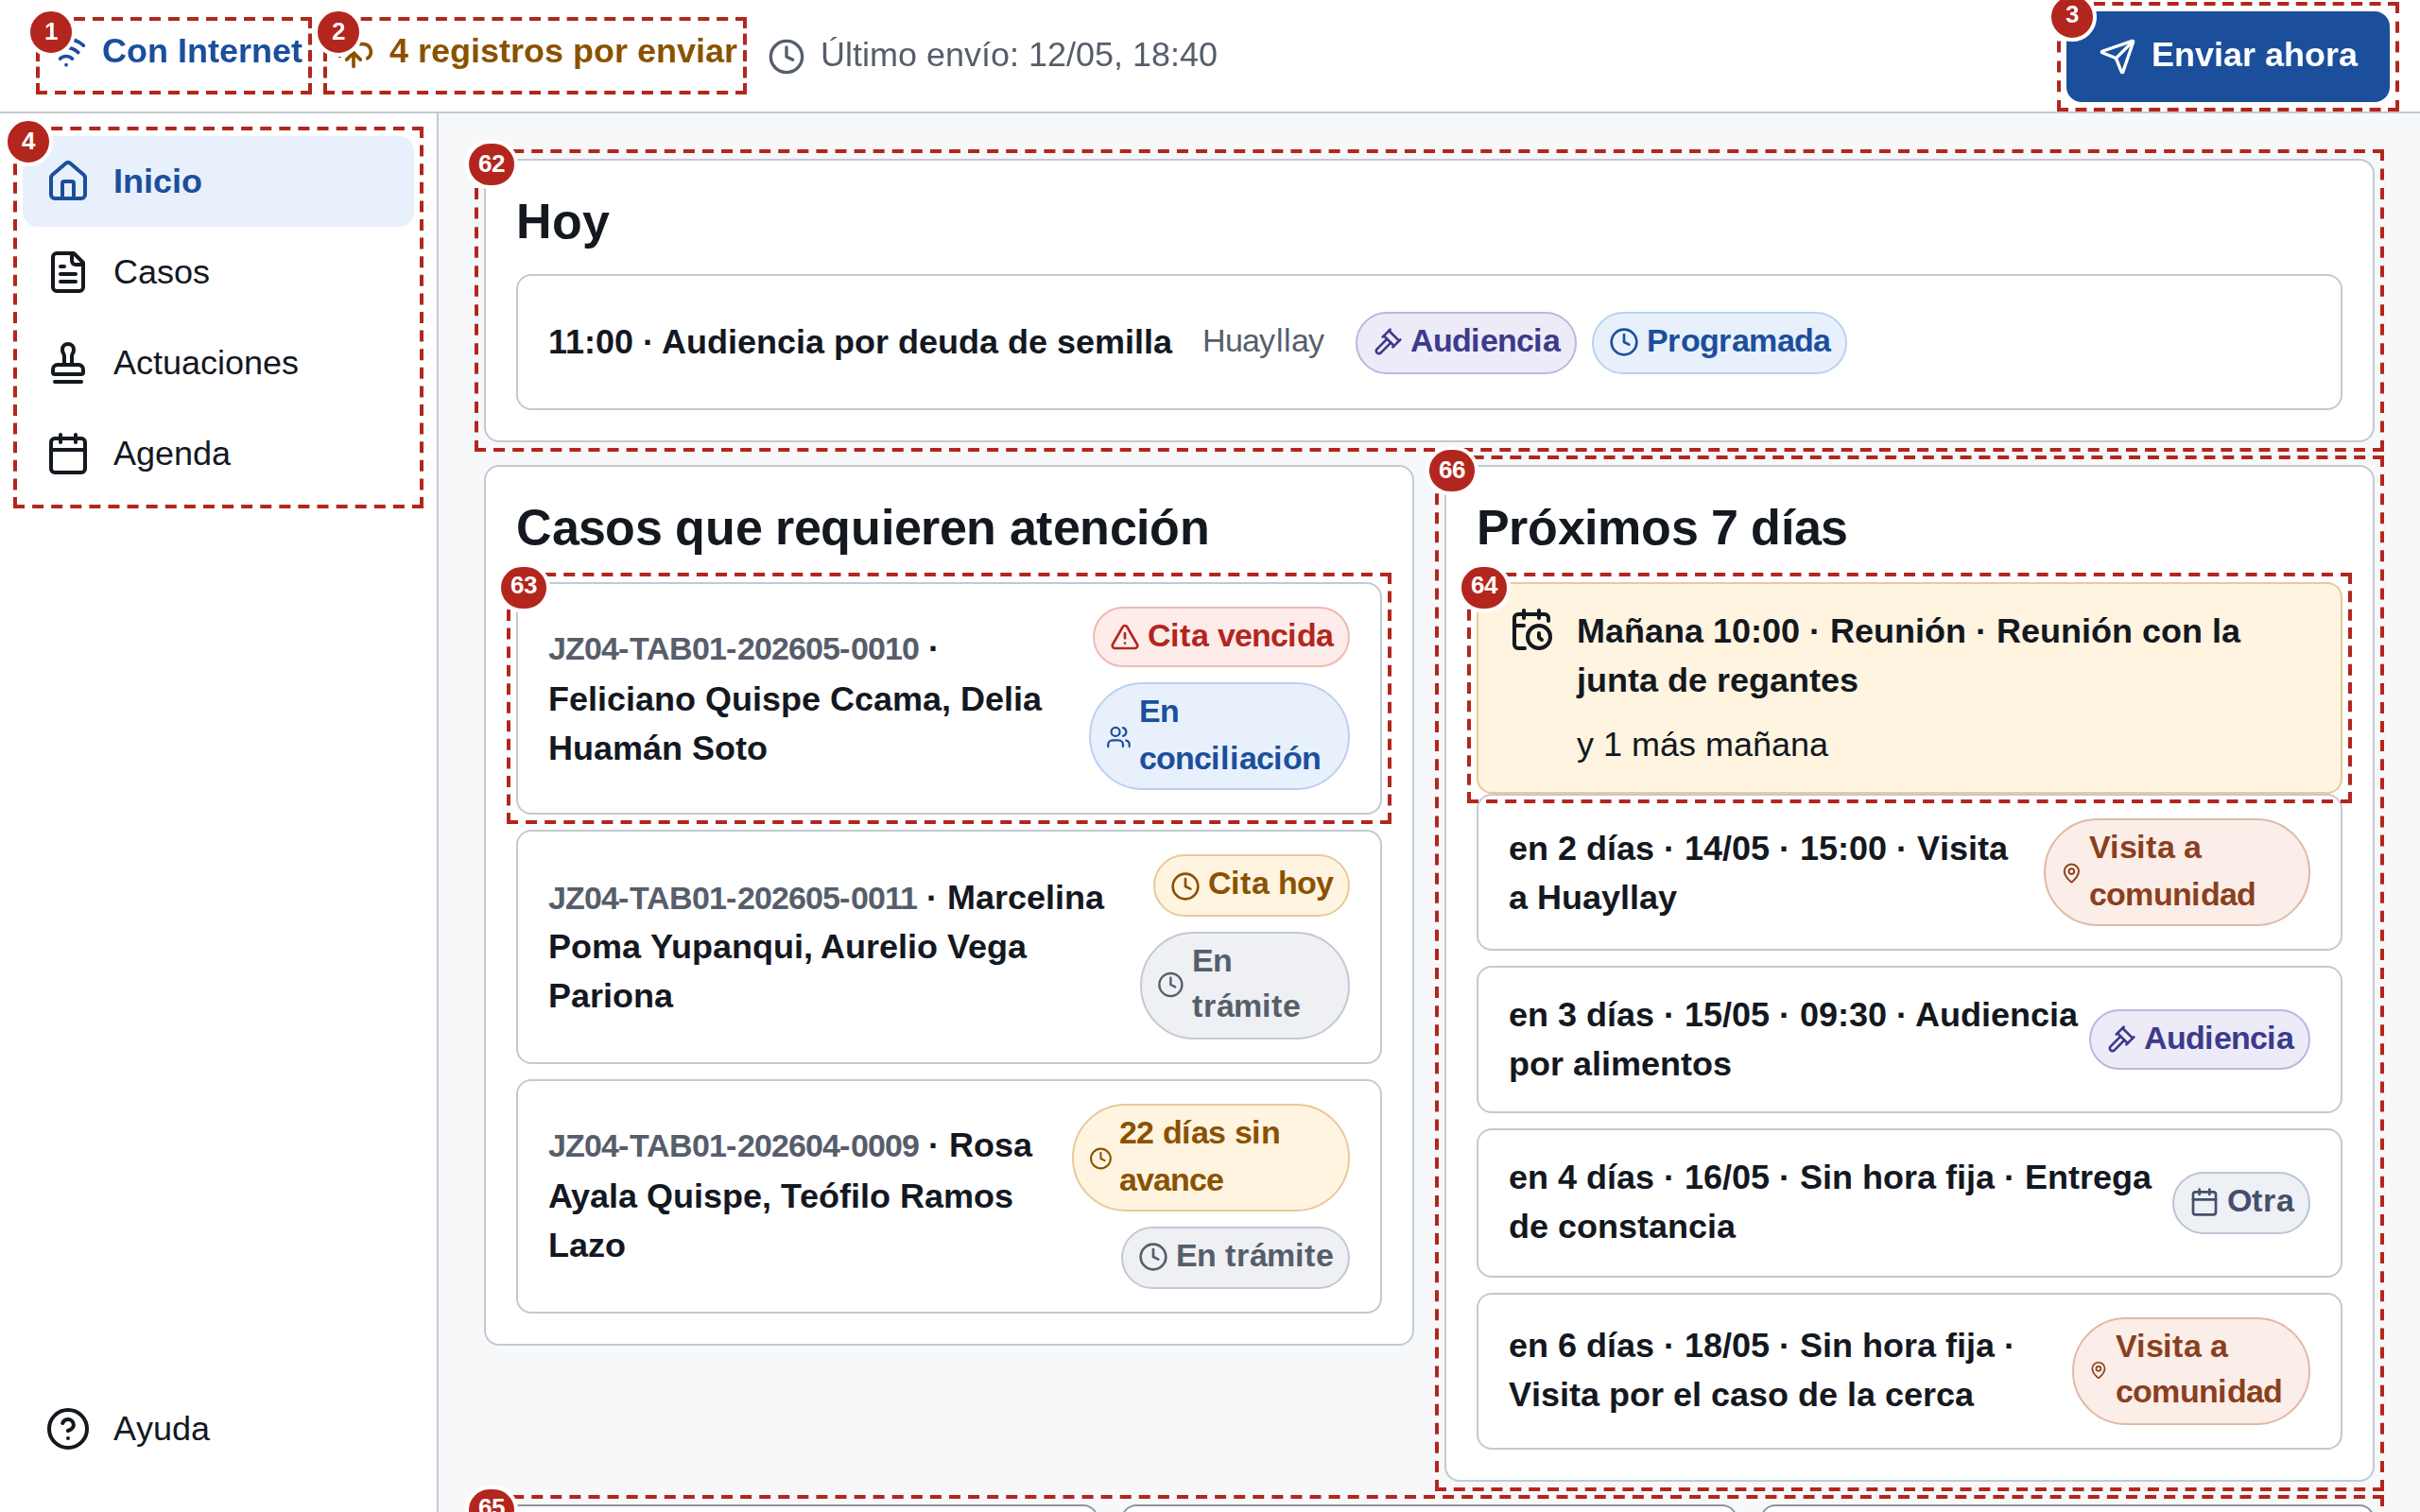
\includegraphics[width=0.86\linewidth]{capturas/A-01_anotada-inicio.png}
\caption{P-01 · Marcadores de la matriz. Cada marcador numerado corresponde a una fila de la matriz de justificación}
\end{figure}
\begin{figure}[H]\centering
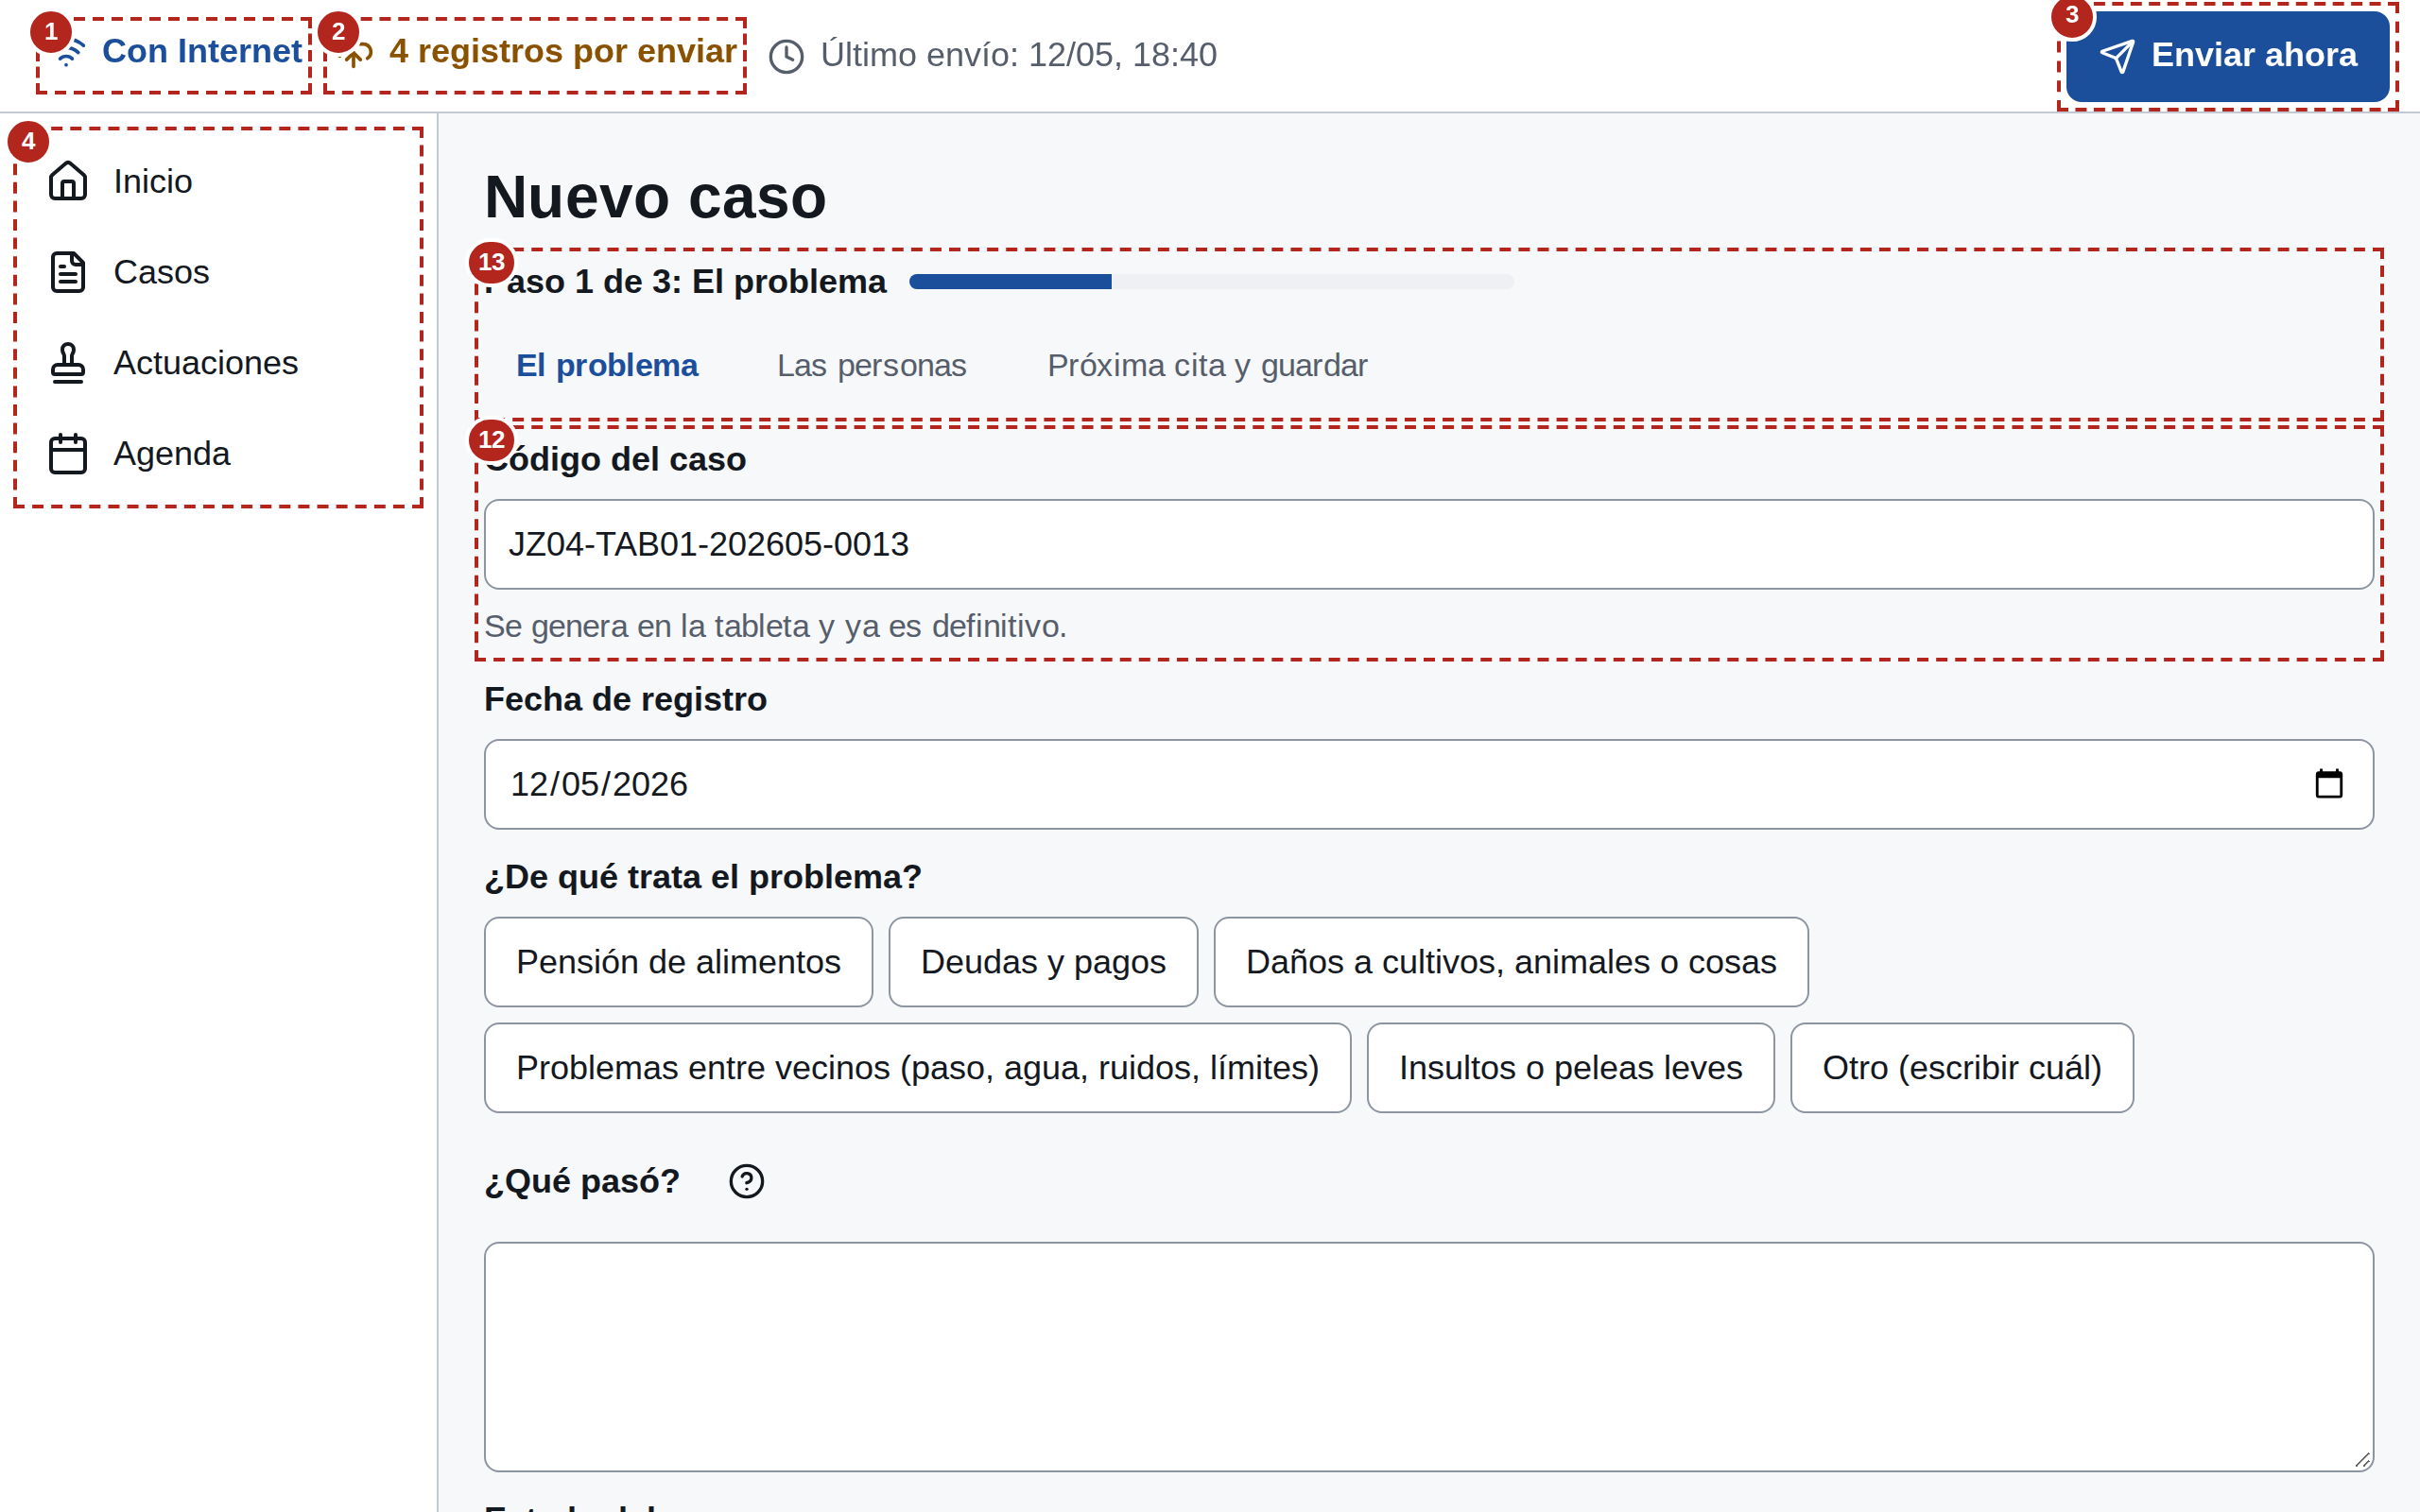
\includegraphics[width=0.86\linewidth]{capturas/A-02_anotada-caso.png}
\caption{P-03 · Marcadores de la matriz. Cada marcador numerado corresponde a una fila de la matriz de justificación}
\end{figure}
\begin{figure}[H]\centering
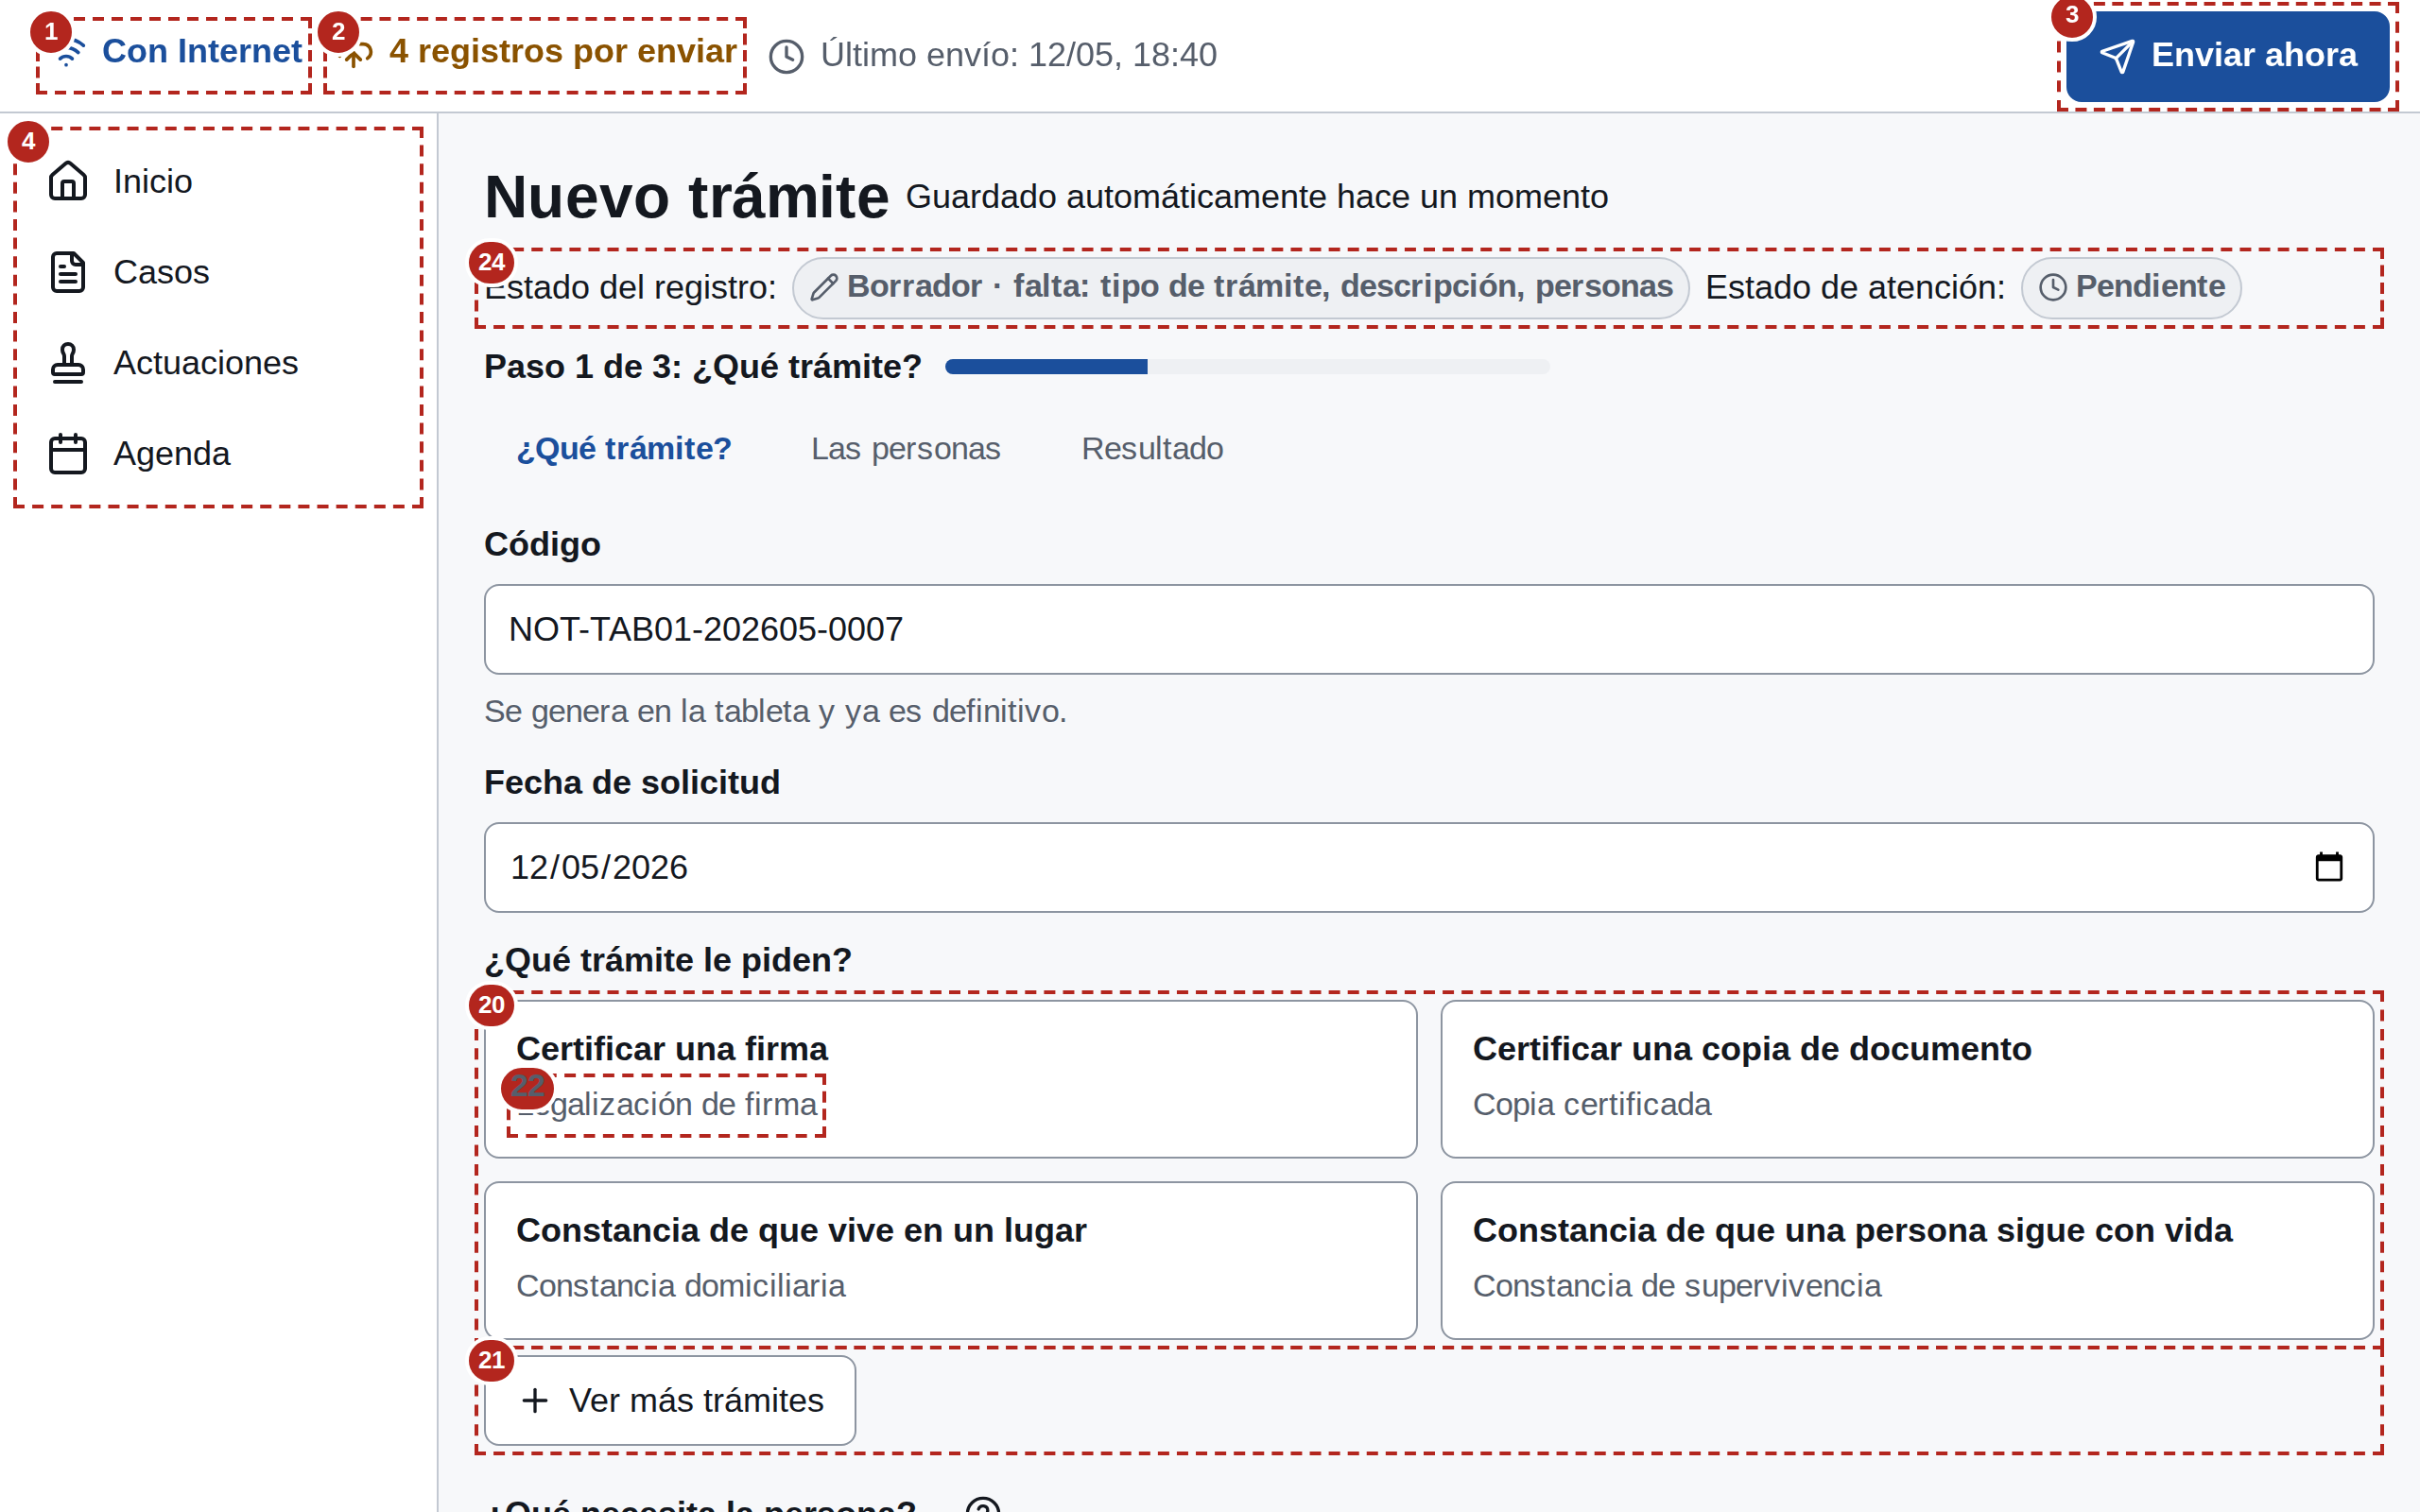
\includegraphics[width=0.86\linewidth]{capturas/A-03_anotada-actuacion.png}
\caption{P-06 · Marcadores de la matriz. Cada marcador numerado corresponde a una fila de la matriz de justificación}
\end{figure}
\begin{figure}[H]\centering
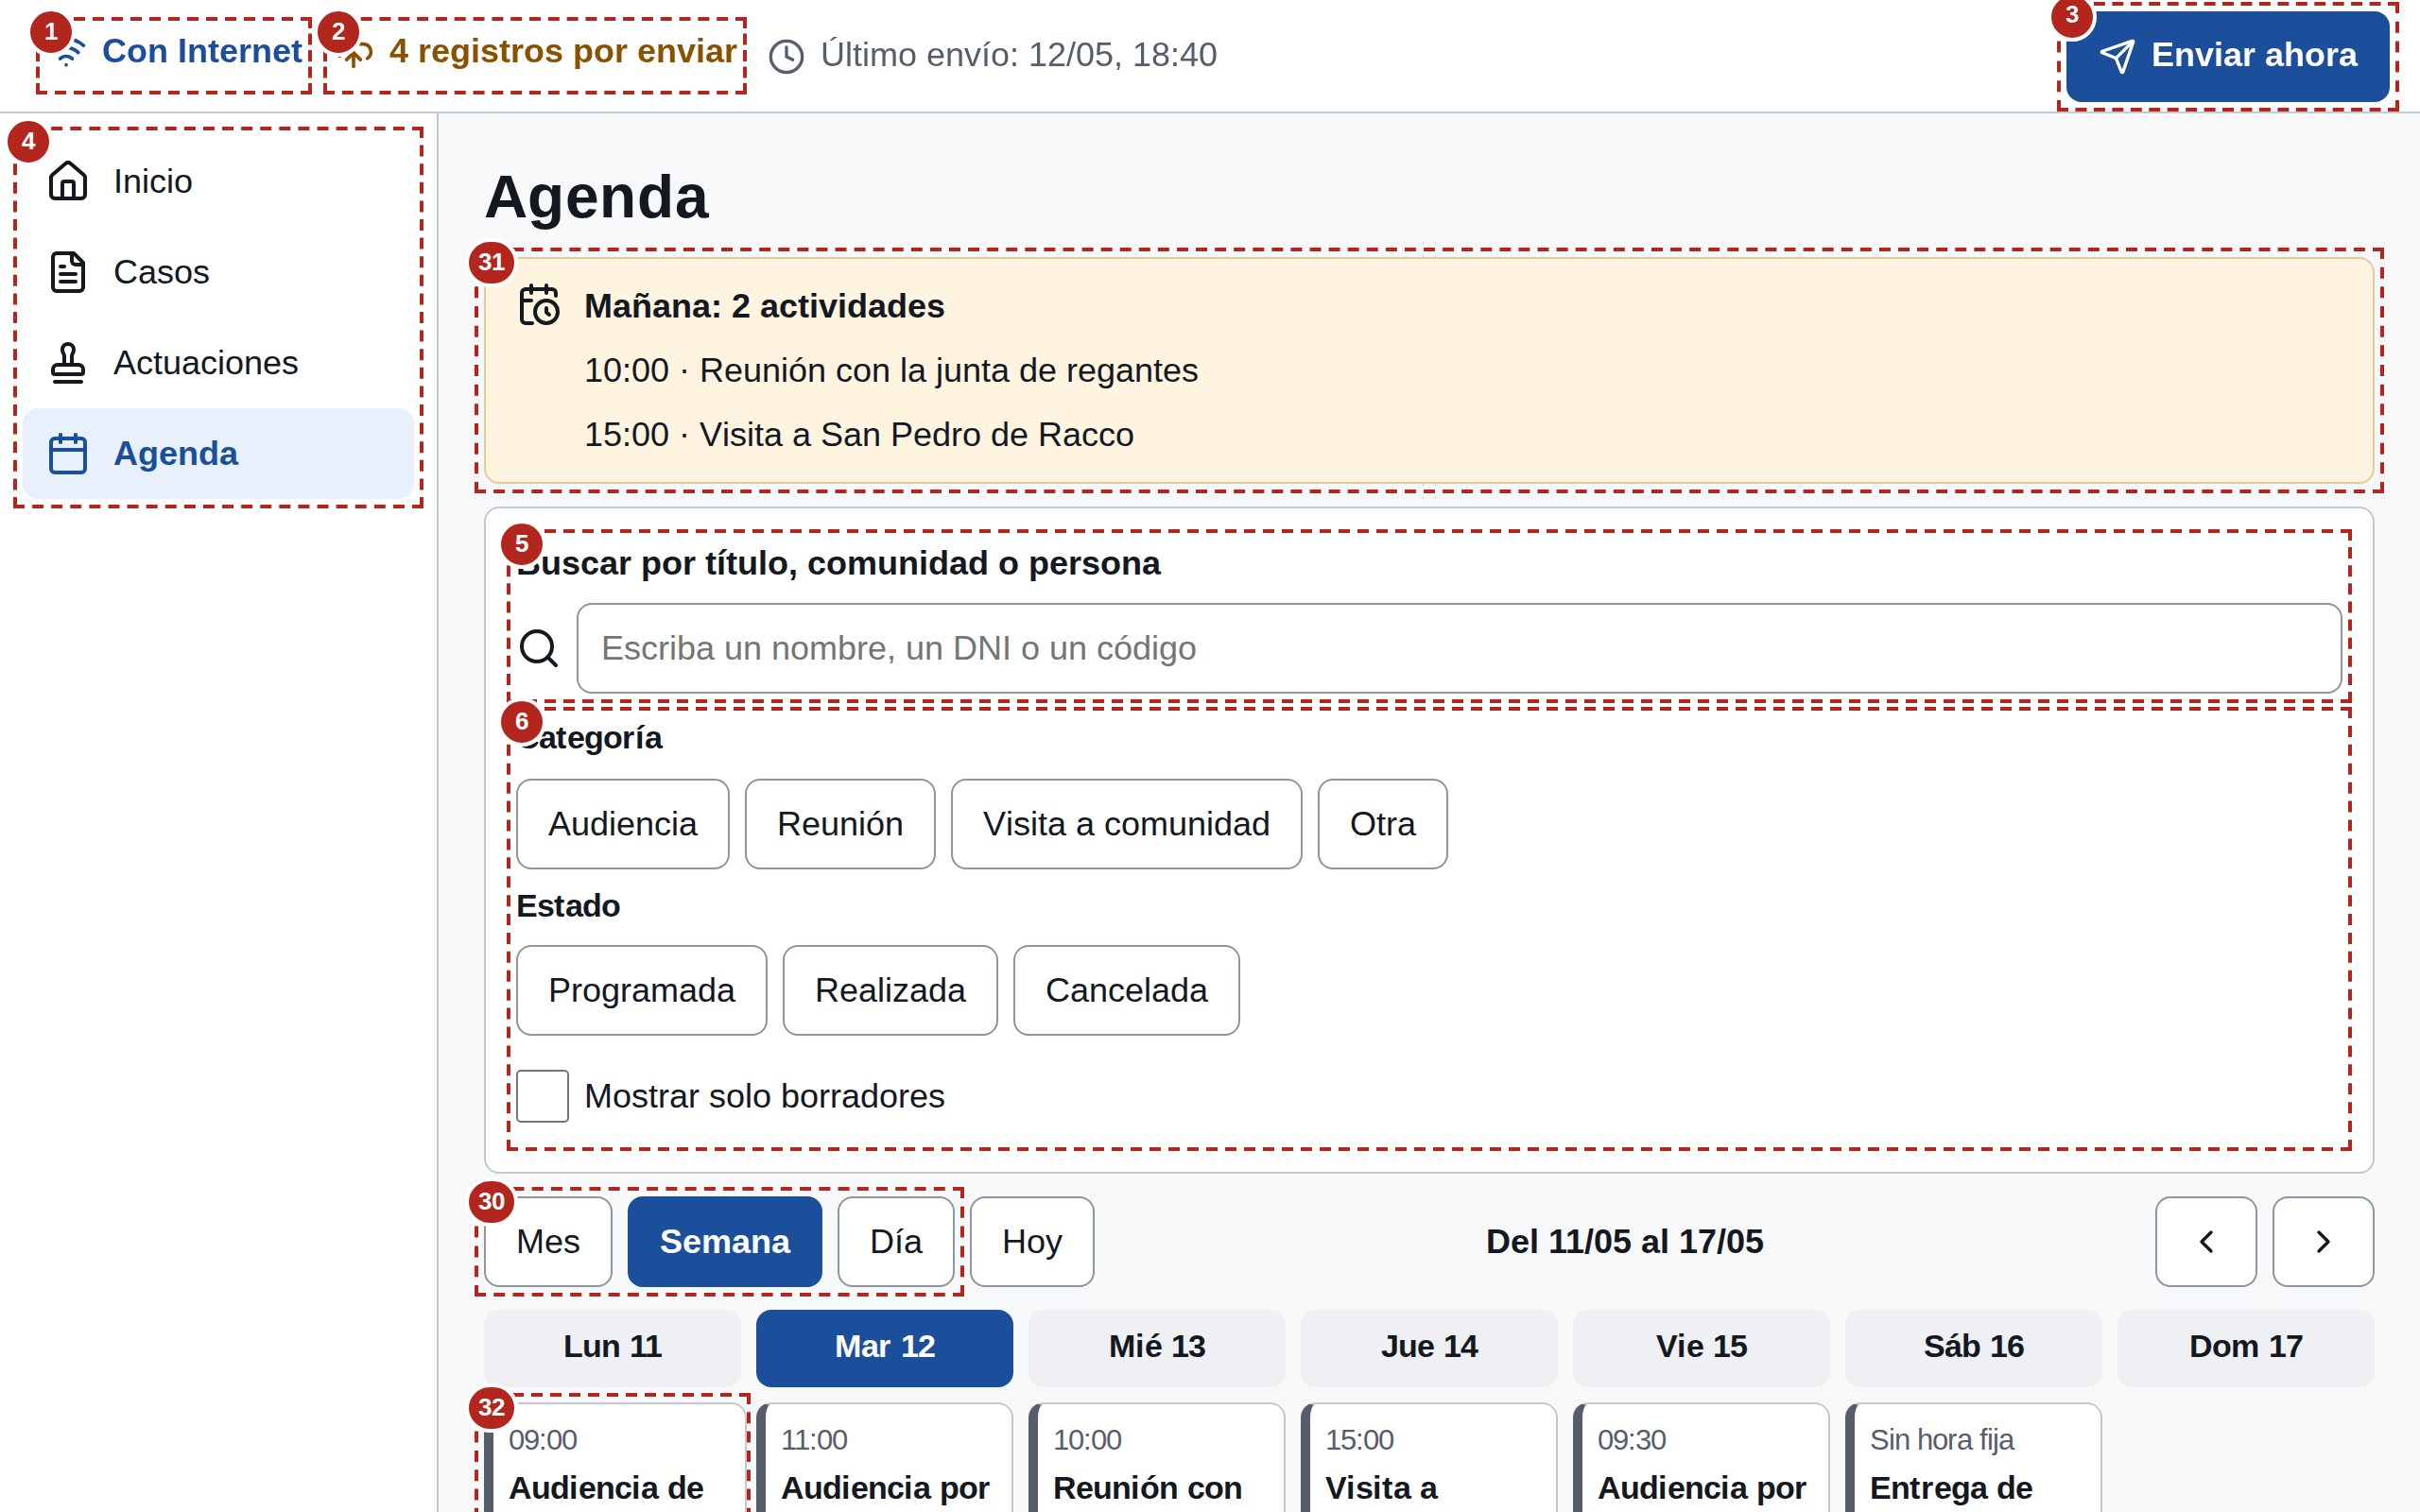
\includegraphics[width=0.86\linewidth]{capturas/A-04_anotada-agenda.png}
\caption{P-07 · Marcadores de la matriz. Cada marcador numerado corresponde a una fila de la matriz de justificación}
\end{figure}
\begin{figure}[H]\centering
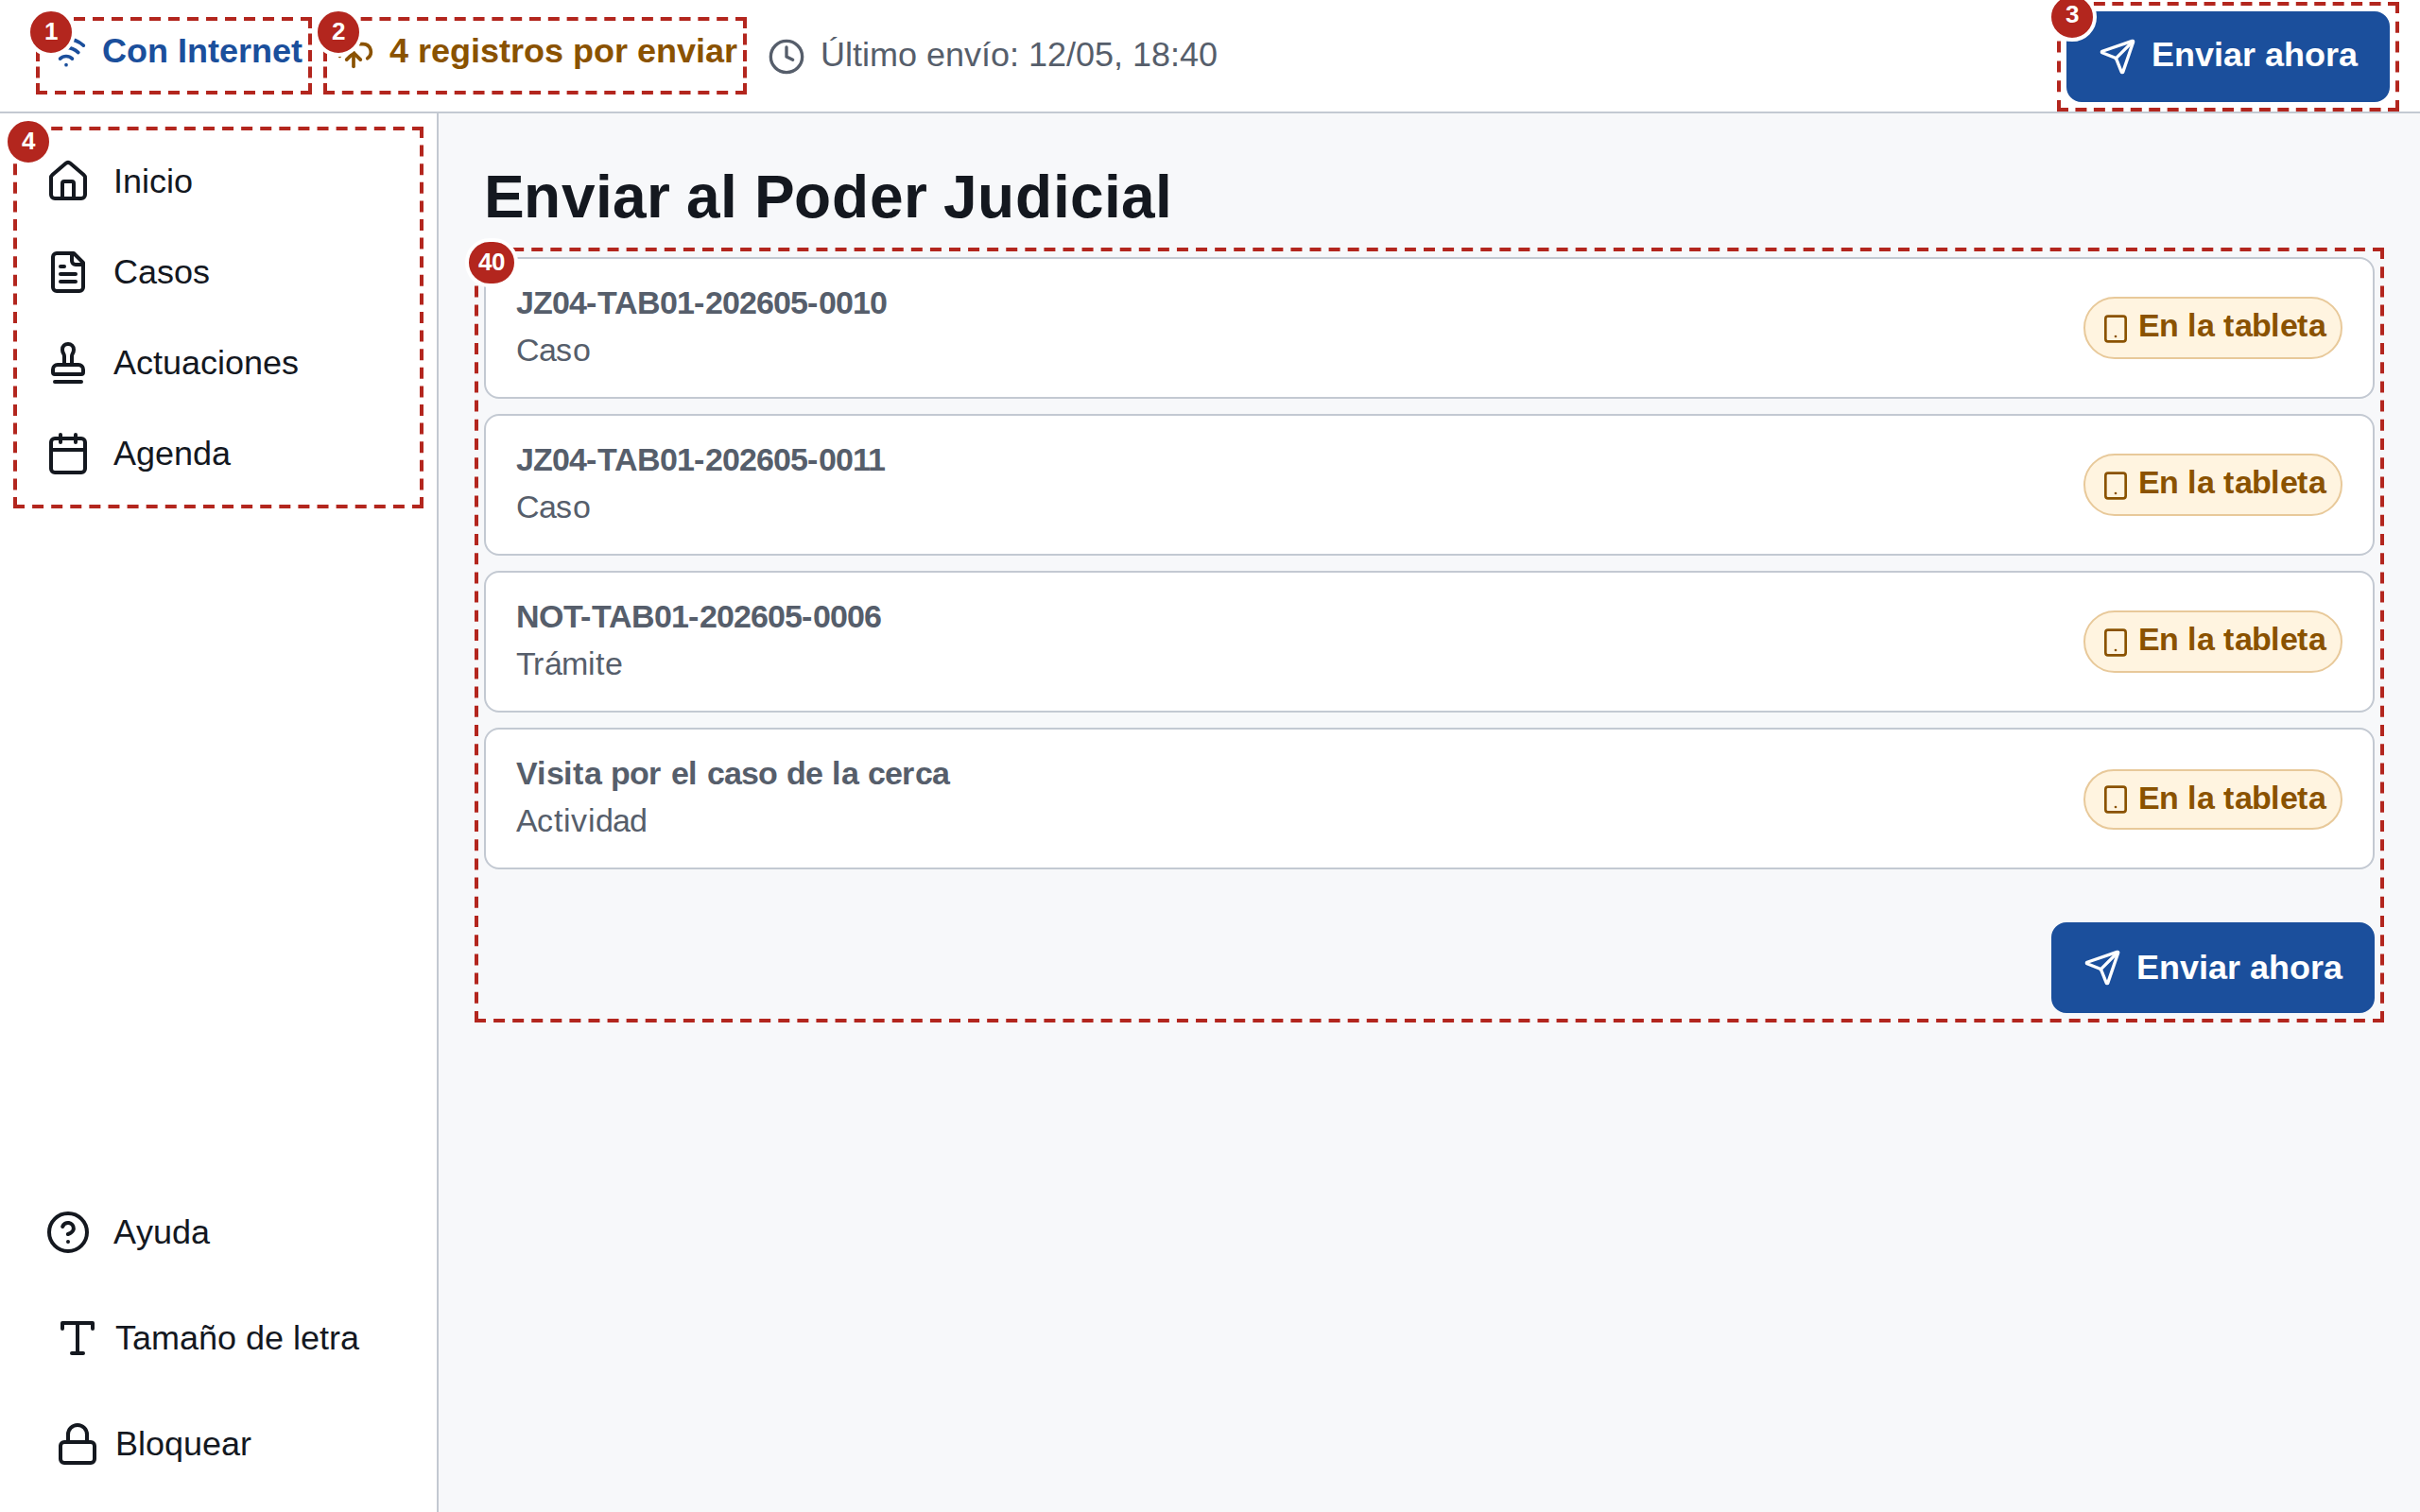
\includegraphics[width=0.86\linewidth]{capturas/A-05_anotada-envio.png}
\caption{P-09 · Marcadores de la matriz. Cada marcador numerado corresponde a una fila de la matriz de justificación}
\end{figure}


\section{Evidencia de factores humanos}

Las dos tablas de esta sección no son estimaciones: las genera Playwright midiendo la aplicación publicada, pantalla por pantalla, y forman parte del repositorio.

\subsection{Objetivos táctiles}

Se midieron todos los botones, enlaces y campos de cada pantalla. El mínimo propio es de 48 por 48 píxeles con 8 píxeles o más de separación, por encima del piso de 44 por 44 que fija WCAG 2.5.5. La medición se repite con cada tamaño de letra (Normal, Grande y Muy grande), porque ahí es donde un diseño ajustado se rompe. El total del texto suma todas las pasadas; la tabla desglosa por pantalla y por tamaño.

Se midieron 486 controles en 12 pantallas, repitiendo la medición con cada tamaño de letra (Normal y Grande). Ninguno queda por debajo de 48 por 48 px ni a menos de 8 px de su vecino.

\small
\setlength{\tabcolsep}{4pt}
\begin{longtable}{@{}p{5.4cm}rrrr@{}}
\toprule
\textbf{Pantalla} & \multicolumn{2}{c}{\textbf{Normal}} & \multicolumn{2}{c}{\textbf{Grande}} \\
 & controles & fallos & controles & fallos \\
\midrule
\endfirsthead
\toprule
\textbf{Pantalla} & \multicolumn{2}{c}{\textbf{Normal}} & \multicolumn{2}{c}{\textbf{Grande}} \\
 & controles & fallos & controles & fallos \\
\midrule
\endhead
\bottomrule
\endfoot
Ayuda Ayuda & 9 & 0 & 9 & 0 \\
P-00 Ingreso con PIN & 12 & 0 & 12 & 0 \\
P-00b Introducción inicial & 2 & 0 & 2 & 0 \\
P-01 Inicio & 19 & 0 & 19 & 0 \\
P-02 Casos: lista y búsqueda & 27 & 0 & 27 & 0 \\
P-03 Caso: nuevo & 28 & 0 & 28 & 0 \\
P-04 Caso: detalle & 10 & 0 & 10 & 0 \\
P-05 Actuaciones: lista y búsqueda & 34 & 0 & 34 & 0 \\
P-06 Actuación: nueva & 23 & 0 & 23 & 0 \\
P-07 Agenda & 32 & 0 & 32 & 0 \\
P-08 Actividad: nueva & 38 & 0 & 38 & 0 \\
P-09 Envío al Poder Judicial & 9 & 0 & 9 & 0 \\
\midrule
\textbf{Total} & \textbf{243} & \textbf{0} & \textbf{243} & \textbf{0} \\
\end{longtable}

\subsection{Contraste}

axe-core midió 526 textos en 13 pantallas contra WCAG 2.1 nivel AA. No se encontró ningún incumplimiento.

\small
\begin{longtable}{@{}p{6.8cm}rrr@{}}
\toprule
\textbf{Pantalla} & \textbf{Textos medidos} & \textbf{Fallos de contraste} & \textbf{Otros fallos AA} \\
\midrule
\endfirsthead
\toprule
\textbf{Pantalla} & \textbf{Textos medidos} & \textbf{Fallos de contraste} & \textbf{Otros fallos AA} \\
\midrule
\endhead
\bottomrule
\endfoot
P-00 Ingreso con PIN & 15 & 0 & 0 \\
P-00b Introducción inicial & 4 & 0 & 0 \\
P-01 Inicio & 42 & 0 & 0 \\
P-02 Casos: lista y búsqueda & 60 & 0 & 0 \\
P-03 Caso: nuevo & 39 & 0 & 0 \\
P-04 Caso: detalle & 37 & 0 & 0 \\
P-05 Actuaciones: lista y búsqueda & 61 & 0 & 0 \\
P-06 Actuación: nueva & 40 & 0 & 0 \\
P-07 Agenda & 79 & 0 & 0 \\
P-08 Actividad: nueva & 54 & 0 & 0 \\
P-09 Envío al Poder Judicial & 25 & 0 & 0 \\
P-10 Vista en computadora & 43 & 0 & 0 \\
Ayuda Ayuda & 27 & 0 & 0 \\
\midrule
\textbf{Total} & \textbf{526} & \textbf{0} & \textbf{0} \\
\end{longtable}

\section{Alcance del prototipo}

\subsection{Lo que funciona de verdad}

El guardado local en el dispositivo, la generación de códigos sin conexión, la detección real de la conexión, la carga de la aplicación sin Internet después de la primera visita, las búsquedas, los filtros, las validaciones, la detección de personas y trámites repetidos, el guardado automático con recuperación, el cálculo de los casos que requieren atención, el aviso de cruce de horarios y el cambio de tamaño de letra.

\subsection{Lo que está simulado}

El servidor del Poder Judicial, el envío y sus resultados, los conflictos entre versiones, el cifrado de los datos locales, el desbloqueo por código telefónico y el nivel de batería. El dictado por voz no es parte del prototipo: depende del teclado del sistema.

\subsection{Por qué no hay botón de micrófono}

La API de voz del navegador envía el audio a un servidor en la mayoría de los casos y fallaría sin Internet, lo que contradiría el mensaje central de la aplicación. En su lugar, los campos de texto largo indican: «Puede hablar en vez de escribir: toque el micrófono del teclado.» La tableta se configura con el teclado del sistema y el paquete de español descargado, que dicta sin Internet. Es configuración del dispositivo, no del prototipo.

\section{Limitaciones y trabajo futuro}

\textbf{Idioma.} La interfaz está en español. Muchos jueces de paz y muchas de las personas que atienden hablan quechua o aimara. Dentro del diseño se mitiga con lenguaje simple, un ícono en cada acción y un resumen legible antes de guardar, pensado para leerlo en voz alta. La línea de trabajo siguiente es la interfaz y las ayudas en quechua y aimara, validadas con usuarios.

\textbf{Orientación.} Solo horizontal, por las razones ya explicadas. Una tableta usada de pie quedaría fuera.

\textbf{Pérdida del dispositivo.} Lo no enviado se pierde si la tableta se pierde o se daña. Por eso existe el recordatorio de los tres días. El cifrado de los datos locales y el borrado remoto están diseñados pero no implementados.

\textbf{Pruebas con usuarios.} Ninguna decisión de este informe está validada con jueces de paz reales. Las justificaciones se apoyan en principios y en las condiciones del caso, no en evidencia de campo.

\end{document}
